\documentclass[twoside]{book}

% Packages required by doxygen
\usepackage{fixltx2e}
\usepackage{calc}
\usepackage{doxygen}
\usepackage[export]{adjustbox} % also loads graphicx
\usepackage{graphicx}
\usepackage[utf8]{inputenc}
\usepackage{makeidx}
\usepackage{multicol}
\usepackage{multirow}
\PassOptionsToPackage{warn}{textcomp}
\usepackage{textcomp}
\usepackage[nointegrals]{wasysym}
\usepackage[table]{xcolor}

% Font selection
\usepackage[T1]{fontenc}
\usepackage[scaled=.90]{helvet}
\usepackage{courier}
\usepackage{amssymb}
\usepackage{sectsty}
\renewcommand{\familydefault}{\sfdefault}
\allsectionsfont{%
  \fontseries{bc}\selectfont%
  \color{darkgray}%
}
\renewcommand{\DoxyLabelFont}{%
  \fontseries{bc}\selectfont%
  \color{darkgray}%
}
\newcommand{\+}{\discretionary{\mbox{\scriptsize$\hookleftarrow$}}{}{}}

% Page & text layout
\usepackage{geometry}
\geometry{%
  a4paper,%
  top=2.5cm,%
  bottom=2.5cm,%
  left=2.5cm,%
  right=2.5cm%
}
\tolerance=750
\hfuzz=15pt
\hbadness=750
\setlength{\emergencystretch}{15pt}
\setlength{\parindent}{0cm}
\setlength{\parskip}{0.2cm}
\makeatletter
\renewcommand{\paragraph}{%
  \@startsection{paragraph}{4}{0ex}{-1.0ex}{1.0ex}{%
    \normalfont\normalsize\bfseries\SS@parafont%
  }%
}
\renewcommand{\subparagraph}{%
  \@startsection{subparagraph}{5}{0ex}{-1.0ex}{1.0ex}{%
    \normalfont\normalsize\bfseries\SS@subparafont%
  }%
}
\makeatother

% Headers & footers
\usepackage{fancyhdr}
\pagestyle{fancyplain}
\fancyhead[LE]{\fancyplain{}{\bfseries\thepage}}
\fancyhead[CE]{\fancyplain{}{}}
\fancyhead[RE]{\fancyplain{}{\bfseries\leftmark}}
\fancyhead[LO]{\fancyplain{}{\bfseries\rightmark}}
\fancyhead[CO]{\fancyplain{}{}}
\fancyhead[RO]{\fancyplain{}{\bfseries\thepage}}
\fancyfoot[LE]{\fancyplain{}{}}
\fancyfoot[CE]{\fancyplain{}{}}
\fancyfoot[RE]{\fancyplain{}{\bfseries\scriptsize Generated on Fri Apr 24 2015 01\+:01\+:47 for Memory\+Oracle by Doxygen }}
\fancyfoot[LO]{\fancyplain{}{\bfseries\scriptsize Generated on Fri Apr 24 2015 01\+:01\+:47 for Memory\+Oracle by Doxygen }}
\fancyfoot[CO]{\fancyplain{}{}}
\fancyfoot[RO]{\fancyplain{}{}}
\renewcommand{\footrulewidth}{0.4pt}
\renewcommand{\chaptermark}[1]{%
  \markboth{#1}{}%
}
\renewcommand{\sectionmark}[1]{%
  \markright{\thesection\ #1}%
}

% Indices & bibliography
\usepackage{natbib}
\usepackage[titles]{tocloft}
\setcounter{tocdepth}{3}
\setcounter{secnumdepth}{5}
\makeindex

% Hyperlinks (required, but should be loaded last)
\usepackage{ifpdf}
\ifpdf
  \usepackage[pdftex,pagebackref=true]{hyperref}
\else
  \usepackage[ps2pdf,pagebackref=true]{hyperref}
\fi
\hypersetup{%
  colorlinks=true,%
  linkcolor=blue,%
  citecolor=blue,%
  unicode%
}

% Custom commands
\newcommand{\clearemptydoublepage}{%
  \newpage{\pagestyle{empty}\cleardoublepage}%
}


%===== C O N T E N T S =====

\begin{document}

% Titlepage & ToC
\hypersetup{pageanchor=false,
             bookmarks=true,
             bookmarksnumbered=true,
             pdfencoding=unicode
            }
\pagenumbering{roman}
\begin{titlepage}
\vspace*{7cm}
\begin{center}%
{\Large Memory\+Oracle \\[1ex]\large -\/1 }\\
\vspace*{1cm}
{\large Generated by Doxygen 1.8.9.1}\\
\vspace*{0.5cm}
{\small Fri Apr 24 2015 01:01:47}\\
\end{center}
\end{titlepage}
\clearemptydoublepage
\tableofcontents
\clearemptydoublepage
\pagenumbering{arabic}
\hypersetup{pageanchor=true}

%--- Begin generated contents ---
\chapter{Namespace Index}
\section{Namespace List}
Here is a list of all namespaces with brief descriptions\+:\begin{DoxyCompactList}
\item\contentsline{section}{\hyperlink{namespacememoryoracle}{memoryoracle} }{\pageref{namespacememoryoracle}}{}
\item\contentsline{section}{\hyperlink{namespacememoryoracle_1_1container}{memoryoracle.\+container} }{\pageref{namespacememoryoracle_1_1container}}{}
\item\contentsline{section}{\hyperlink{namespacememoryoracle_1_1descriptions}{memoryoracle.\+descriptions} }{\pageref{namespacememoryoracle_1_1descriptions}}{}
\item\contentsline{section}{\hyperlink{namespacememoryoracle_1_1execution}{memoryoracle.\+execution} }{\pageref{namespacememoryoracle_1_1execution}}{}
\item\contentsline{section}{\hyperlink{namespacememoryoracle_1_1frame}{memoryoracle.\+frame} }{\pageref{namespacememoryoracle_1_1frame}}{}
\item\contentsline{section}{\hyperlink{namespacememoryoracle_1_1instance}{memoryoracle.\+instance} }{\pageref{namespacememoryoracle_1_1instance}}{}
\item\contentsline{section}{\hyperlink{namespacememoryoracle_1_1migrations}{memoryoracle.\+migrations} }{\pageref{namespacememoryoracle_1_1migrations}}{}
\item\contentsline{section}{\hyperlink{namespacememoryoracle_1_1migrations_1_10001__initial}{memoryoracle.\+migrations.\+0001\+\_\+initial} }{\pageref{namespacememoryoracle_1_1migrations_1_10001__initial}}{}
\item\contentsline{section}{\hyperlink{namespacememoryoracle_1_1migrations_1_10002__auto__20150402__2000}{memoryoracle.\+migrations.\+0002\+\_\+auto\+\_\+20150402\+\_\+2000} }{\pageref{namespacememoryoracle_1_1migrations_1_10002__auto__20150402__2000}}{}
\item\contentsline{section}{\hyperlink{namespacememoryoracle_1_1migrations_1_10003__auto__20150402__2000}{memoryoracle.\+migrations.\+0003\+\_\+auto\+\_\+20150402\+\_\+2000} }{\pageref{namespacememoryoracle_1_1migrations_1_10003__auto__20150402__2000}}{}
\item\contentsline{section}{\hyperlink{namespacememoryoracle_1_1migrations_1_10004__auto__20150402__2000}{memoryoracle.\+migrations.\+0004\+\_\+auto\+\_\+20150402\+\_\+2000} }{\pageref{namespacememoryoracle_1_1migrations_1_10004__auto__20150402__2000}}{}
\item\contentsline{section}{\hyperlink{namespacememoryoracle_1_1migrations_1_10005__auto__20150403__0100}{memoryoracle.\+migrations.\+0005\+\_\+auto\+\_\+20150403\+\_\+0100} }{\pageref{namespacememoryoracle_1_1migrations_1_10005__auto__20150403__0100}}{}
\item\contentsline{section}{\hyperlink{namespacememoryoracle_1_1migrations_1_10006__program__path}{memoryoracle.\+migrations.\+0006\+\_\+program\+\_\+path} }{\pageref{namespacememoryoracle_1_1migrations_1_10006__program__path}}{}
\item\contentsline{section}{\hyperlink{namespacememoryoracle_1_1migrations_1_10007__auto__20150403__0248}{memoryoracle.\+migrations.\+0007\+\_\+auto\+\_\+20150403\+\_\+0248} }{\pageref{namespacememoryoracle_1_1migrations_1_10007__auto__20150403__0248}}{}
\item\contentsline{section}{\hyperlink{namespacememoryoracle_1_1models}{memoryoracle.\+models} }{\pageref{namespacememoryoracle_1_1models}}{}
\item\contentsline{section}{\hyperlink{namespacememoryoracle_1_1registry}{memoryoracle.\+registry} }{\pageref{namespacememoryoracle_1_1registry}}{}
\item\contentsline{section}{\hyperlink{namespacememoryoracle_1_1settings}{memoryoracle.\+settings} }{\pageref{namespacememoryoracle_1_1settings}}{}
\item\contentsline{section}{\hyperlink{namespacememoryoracle_1_1symbol}{memoryoracle.\+symbol} }{\pageref{namespacememoryoracle_1_1symbol}}{}
\item\contentsline{section}{\hyperlink{namespacememoryoracle_1_1test__models}{memoryoracle.\+test\+\_\+models} }{\pageref{namespacememoryoracle_1_1test__models}}{}
\item\contentsline{section}{\hyperlink{namespacememoryoracle_1_1tracked}{memoryoracle.\+tracked} }{\pageref{namespacememoryoracle_1_1tracked}}{}
\item\contentsline{section}{\hyperlink{namespacememoryoracle_1_1typed}{memoryoracle.\+typed} }{\pageref{namespacememoryoracle_1_1typed}}{}
\item\contentsline{section}{\hyperlink{namespacememoryoracle_1_1urls}{memoryoracle.\+urls} }{\pageref{namespacememoryoracle_1_1urls}}{}
\item\contentsline{section}{\hyperlink{namespacememoryoracle_1_1watch}{memoryoracle.\+watch} }{\pageref{namespacememoryoracle_1_1watch}}{}
\item\contentsline{section}{\hyperlink{namespacememoryoracle_1_1whip}{memoryoracle.\+whip} }{\pageref{namespacememoryoracle_1_1whip}}{}
\item\contentsline{section}{\hyperlink{namespacememoryoracle_1_1wsgi}{memoryoracle.\+wsgi} }{\pageref{namespacememoryoracle_1_1wsgi}}{}
\end{DoxyCompactList}

\chapter{Hierarchical Index}
\section{Class Hierarchy}
This inheritance list is sorted roughly, but not completely, alphabetically\+:\begin{DoxyCompactList}
\item Breakpoint\begin{DoxyCompactList}
\item \contentsline{section}{memoryoracle.\+instance.\+Memory\+Watcher}{\pageref{classmemoryoracle_1_1instance_1_1MemoryWatcher}}{}
\item \contentsline{section}{memoryoracle.\+watch.\+Addressable\+Watcher}{\pageref{classmemoryoracle_1_1watch_1_1AddressableWatcher}}{}
\item \contentsline{section}{memoryoracle.\+watch.\+State\+Catch}{\pageref{classmemoryoracle_1_1watch_1_1StateCatch}}{}
\end{DoxyCompactList}
\item Document\begin{DoxyCompactList}
\item \contentsline{section}{memoryoracle.\+execution.\+Commit}{\pageref{classmemoryoracle_1_1execution_1_1Commit}}{}
\item \contentsline{section}{memoryoracle.\+execution.\+Execution}{\pageref{classmemoryoracle_1_1execution_1_1Execution}}{}
\item \contentsline{section}{memoryoracle.\+execution.\+Instance}{\pageref{classmemoryoracle_1_1execution_1_1Instance}}{}
\item \contentsline{section}{memoryoracle.\+tracked.\+Tracked}{\pageref{classmemoryoracle_1_1tracked_1_1Tracked}}{}
\begin{DoxyCompactList}
\item \contentsline{section}{memoryoracle.\+tracked.\+Owner}{\pageref{classmemoryoracle_1_1tracked_1_1Owner}}{}
\item \contentsline{section}{memoryoracle.\+tracked.\+Program\+File}{\pageref{classmemoryoracle_1_1tracked_1_1ProgramFile}}{}
\begin{DoxyCompactList}
\item \contentsline{section}{memoryoracle.\+tracked.\+Object\+File}{\pageref{classmemoryoracle_1_1tracked_1_1ObjectFile}}{}
\item \contentsline{section}{memoryoracle.\+tracked.\+Source\+File}{\pageref{classmemoryoracle_1_1tracked_1_1SourceFile}}{}
\end{DoxyCompactList}
\item \contentsline{section}{memoryoracle.\+tracked.\+Reference}{\pageref{classmemoryoracle_1_1tracked_1_1Reference}}{}
\item \contentsline{section}{memoryoracle.\+tracked.\+Untracked\+Decorator}{\pageref{classmemoryoracle_1_1tracked_1_1UntrackedDecorator}}{}
\item \contentsline{section}{memoryoracle.\+typed.\+Typed}{\pageref{classmemoryoracle_1_1typed_1_1Typed}}{}
\begin{DoxyCompactList}
\item \contentsline{section}{memoryoracle.\+instance.\+Memory}{\pageref{classmemoryoracle_1_1instance_1_1Memory}}{}
\begin{DoxyCompactList}
\item \contentsline{section}{memoryoracle.\+instance.\+Array}{\pageref{classmemoryoracle_1_1instance_1_1Array}}{}
\item \contentsline{section}{memoryoracle.\+instance.\+Call}{\pageref{classmemoryoracle_1_1instance_1_1Call}}{}
\item \contentsline{section}{memoryoracle.\+instance.\+Const\+Decorator}{\pageref{classmemoryoracle_1_1instance_1_1ConstDecorator}}{}
\item \contentsline{section}{memoryoracle.\+instance.\+Extern\+Decorator}{\pageref{classmemoryoracle_1_1instance_1_1ExternDecorator}}{}
\item \contentsline{section}{memoryoracle.\+instance.\+Member\+Decorator}{\pageref{classmemoryoracle_1_1instance_1_1MemberDecorator}}{}
\item \contentsline{section}{memoryoracle.\+instance.\+Primitive}{\pageref{classmemoryoracle_1_1instance_1_1Primitive}}{}
\begin{DoxyCompactList}
\item \contentsline{section}{memoryoracle.\+instance.\+Float}{\pageref{classmemoryoracle_1_1instance_1_1Float}}{}
\item \contentsline{section}{memoryoracle.\+instance.\+Int}{\pageref{classmemoryoracle_1_1instance_1_1Int}}{}
\item \contentsline{section}{memoryoracle.\+instance.\+Pointer}{\pageref{classmemoryoracle_1_1instance_1_1Pointer}}{}
\item \contentsline{section}{memoryoracle.\+instance.\+Char\+String}{\pageref{classmemoryoracle_1_1instance_1_1CharString}}{}
\end{DoxyCompactList}
\item \contentsline{section}{memoryoracle.\+instance.\+Register\+Decorator}{\pageref{classmemoryoracle_1_1instance_1_1RegisterDecorator}}{}
\item \contentsline{section}{memoryoracle.\+instance.\+Static\+Decorator}{\pageref{classmemoryoracle_1_1instance_1_1StaticDecorator}}{}
\item \contentsline{section}{memoryoracle.\+instance.\+Structure}{\pageref{classmemoryoracle_1_1instance_1_1Structure}}{}
\item \contentsline{section}{memoryoracle.\+instance.\+Void}{\pageref{classmemoryoracle_1_1instance_1_1Void}}{}
\item \contentsline{section}{memoryoracle.\+instance.\+Volatile\+Decorator}{\pageref{classmemoryoracle_1_1instance_1_1VolatileDecorator}}{}
\end{DoxyCompactList}
\item \contentsline{section}{memoryoracle.\+symbol.\+Symbol}{\pageref{classmemoryoracle_1_1symbol_1_1Symbol}}{}
\begin{DoxyCompactList}
\item \contentsline{section}{memoryoracle.\+symbol.\+Alias}{\pageref{classmemoryoracle_1_1symbol_1_1Alias}}{}
\begin{DoxyCompactList}
\item \contentsline{section}{memoryoracle.\+symbol.\+Typedef}{\pageref{classmemoryoracle_1_1symbol_1_1Typedef}}{}
\end{DoxyCompactList}
\item \contentsline{section}{memoryoracle.\+symbol.\+Function}{\pageref{classmemoryoracle_1_1symbol_1_1Function}}{}
\item \contentsline{section}{memoryoracle.\+symbol.\+Namespace}{\pageref{classmemoryoracle_1_1symbol_1_1Namespace}}{}
\item \contentsline{section}{memoryoracle.\+symbol.\+Template\+Decorator}{\pageref{classmemoryoracle_1_1symbol_1_1TemplateDecorator}}{}
\begin{DoxyCompactList}
\item \contentsline{section}{memoryoracle.\+symbol.\+Templated\+Decorator}{\pageref{classmemoryoracle_1_1symbol_1_1TemplatedDecorator}}{}
\end{DoxyCompactList}
\item \contentsline{section}{memoryoracle.\+symbol.\+Type}{\pageref{classmemoryoracle_1_1symbol_1_1Type}}{}
\begin{DoxyCompactList}
\item \contentsline{section}{memoryoracle.\+symbol.\+Enum}{\pageref{classmemoryoracle_1_1symbol_1_1Enum}}{}
\item \contentsline{section}{memoryoracle.\+symbol.\+Simple\+Type}{\pageref{classmemoryoracle_1_1symbol_1_1SimpleType}}{}
\item \contentsline{section}{memoryoracle.\+symbol.\+Structure}{\pageref{classmemoryoracle_1_1symbol_1_1Structure}}{}
\item \contentsline{section}{memoryoracle.\+symbol.\+Strongly\+Typed\+Enum}{\pageref{classmemoryoracle_1_1symbol_1_1StronglyTypedEnum}}{}
\item \contentsline{section}{memoryoracle.\+symbol.\+Union}{\pageref{classmemoryoracle_1_1symbol_1_1Union}}{}
\end{DoxyCompactList}
\item \contentsline{section}{memoryoracle.\+symbol.\+Variable}{\pageref{classmemoryoracle_1_1symbol_1_1Variable}}{}
\end{DoxyCompactList}
\end{DoxyCompactList}
\end{DoxyCompactList}
\end{DoxyCompactList}
\item Embedded\+Document\begin{DoxyCompactList}
\item \contentsline{section}{memoryoracle.\+execution.\+Executable}{\pageref{classmemoryoracle_1_1execution_1_1Executable}}{}
\end{DoxyCompactList}
\item Exception\begin{DoxyCompactList}
\item \contentsline{section}{memoryoracle.\+instance.\+Memory.\+Duplicate\+Address}{\pageref{classmemoryoracle_1_1instance_1_1Memory_1_1DuplicateAddress}}{}
\item \contentsline{section}{memoryoracle.\+models.\+Typed.\+Data\+Error}{\pageref{classmemoryoracle_1_1models_1_1Typed_1_1DataError}}{}
\item \contentsline{section}{memoryoracle.\+models.\+Typed.\+Detection\+Error}{\pageref{classmemoryoracle_1_1models_1_1Typed_1_1DetectionError}}{}
\item \contentsline{section}{memoryoracle.\+registry.\+Type\+Detection\+Error}{\pageref{classmemoryoracle_1_1registry_1_1TypeDetectionError}}{}
\end{DoxyCompactList}
\item Finish\+Breakpoint\begin{DoxyCompactList}
\item \contentsline{section}{memoryoracle.\+watch.\+Frame\+Finish}{\pageref{classmemoryoracle_1_1watch_1_1FrameFinish}}{}
\end{DoxyCompactList}
\item J\+S\+O\+N\+Encoder\begin{DoxyCompactList}
\item \contentsline{section}{memoryoracle.\+instance.\+State\+Serializer}{\pageref{classmemoryoracle_1_1instance_1_1StateSerializer}}{}
\end{DoxyCompactList}
\item \contentsline{section}{memoryoracle.\+models.\+Execution.\+Meta}{\pageref{classmemoryoracle_1_1models_1_1Execution_1_1Meta}}{}
\item \contentsline{section}{memoryoracle.\+models.\+Typed.\+Meta}{\pageref{classmemoryoracle_1_1models_1_1Typed_1_1Meta}}{}
\item \contentsline{section}{memoryoracle.\+models.\+Memory.\+Meta}{\pageref{classmemoryoracle_1_1models_1_1Memory_1_1Meta}}{}
\item \contentsline{section}{memoryoracle.\+models.\+Program\+File.\+Meta}{\pageref{classmemoryoracle_1_1models_1_1ProgramFile_1_1Meta}}{}
\item \contentsline{section}{memoryoracle.\+models.\+Object\+File.\+Meta}{\pageref{classmemoryoracle_1_1models_1_1ObjectFile_1_1Meta}}{}
\item \contentsline{section}{memoryoracle.\+models.\+Source\+File.\+Meta}{\pageref{classmemoryoracle_1_1models_1_1SourceFile_1_1Meta}}{}
\item \contentsline{section}{memoryoracle.\+models.\+Symbol.\+Meta}{\pageref{classmemoryoracle_1_1models_1_1Symbol_1_1Meta}}{}
\item \contentsline{section}{memoryoracle.\+models.\+Type.\+Meta}{\pageref{classmemoryoracle_1_1models_1_1Type_1_1Meta}}{}
\item \contentsline{section}{memoryoracle.\+models.\+Tracked.\+Meta}{\pageref{classmemoryoracle_1_1models_1_1Tracked_1_1Meta}}{}
\item \contentsline{section}{memoryoracle.\+models.\+Program.\+Meta}{\pageref{classmemoryoracle_1_1models_1_1Program_1_1Meta}}{}
\item \contentsline{section}{memoryoracle.\+models.\+Commit.\+Meta}{\pageref{classmemoryoracle_1_1models_1_1Commit_1_1Meta}}{}
\item \contentsline{section}{memoryoracle.\+models.\+Executable.\+Meta}{\pageref{classmemoryoracle_1_1models_1_1Executable_1_1Meta}}{}
\item Migration\begin{DoxyCompactList}
\item \contentsline{section}{memoryoracle.\+migrations.0001\+\_\+initial.Migration}{\pageref{classmemoryoracle_1_1migrations_1_10001__initial_1_1Migration}}{}
\item \contentsline{section}{memoryoracle.\+migrations.0002\+\_\+auto\+\_\+20150402\+\_\+2000.Migration}{\pageref{classmemoryoracle_1_1migrations_1_10002__auto__20150402__2000_1_1Migration}}{}
\item \contentsline{section}{memoryoracle.\+migrations.0003\+\_\+auto\+\_\+20150402\+\_\+2000.Migration}{\pageref{classmemoryoracle_1_1migrations_1_10003__auto__20150402__2000_1_1Migration}}{}
\item \contentsline{section}{memoryoracle.\+migrations.0004\+\_\+auto\+\_\+20150402\+\_\+2000.Migration}{\pageref{classmemoryoracle_1_1migrations_1_10004__auto__20150402__2000_1_1Migration}}{}
\item \contentsline{section}{memoryoracle.\+migrations.0005\+\_\+auto\+\_\+20150403\+\_\+0100.Migration}{\pageref{classmemoryoracle_1_1migrations_1_10005__auto__20150403__0100_1_1Migration}}{}
\item \contentsline{section}{memoryoracle.\+migrations.0006\+\_\+program\+\_\+path.Migration}{\pageref{classmemoryoracle_1_1migrations_1_10006__program__path_1_1Migration}}{}
\item \contentsline{section}{memoryoracle.\+migrations.0007\+\_\+auto\+\_\+20150403\+\_\+0248.Migration}{\pageref{classmemoryoracle_1_1migrations_1_10007__auto__20150403__0248_1_1Migration}}{}
\end{DoxyCompactList}
\item Model\begin{DoxyCompactList}
\item \contentsline{section}{memoryoracle.\+models.\+Tracked}{\pageref{classmemoryoracle_1_1models_1_1Tracked}}{}
\begin{DoxyCompactList}
\item \contentsline{section}{memoryoracle.\+models.\+Commit}{\pageref{classmemoryoracle_1_1models_1_1Commit}}{}
\item \contentsline{section}{memoryoracle.\+models.\+Executable}{\pageref{classmemoryoracle_1_1models_1_1Executable}}{}
\item \contentsline{section}{memoryoracle.\+models.\+Execution}{\pageref{classmemoryoracle_1_1models_1_1Execution}}{}
\item \contentsline{section}{memoryoracle.\+models.\+Program}{\pageref{classmemoryoracle_1_1models_1_1Program}}{}
\item \contentsline{section}{memoryoracle.\+models.\+Program\+File}{\pageref{classmemoryoracle_1_1models_1_1ProgramFile}}{}
\begin{DoxyCompactList}
\item \contentsline{section}{memoryoracle.\+models.\+Object\+File}{\pageref{classmemoryoracle_1_1models_1_1ObjectFile}}{}
\item \contentsline{section}{memoryoracle.\+models.\+Source\+File}{\pageref{classmemoryoracle_1_1models_1_1SourceFile}}{}
\end{DoxyCompactList}
\item \contentsline{section}{memoryoracle.\+models.\+Type}{\pageref{classmemoryoracle_1_1models_1_1Type}}{}
\item \contentsline{section}{memoryoracle.\+models.\+Typed}{\pageref{classmemoryoracle_1_1models_1_1Typed}}{}
\begin{DoxyCompactList}
\item \contentsline{section}{memoryoracle.\+models.\+Memory}{\pageref{classmemoryoracle_1_1models_1_1Memory}}{}
\item \contentsline{section}{memoryoracle.\+models.\+Symbol}{\pageref{classmemoryoracle_1_1models_1_1Symbol}}{}
\end{DoxyCompactList}
\end{DoxyCompactList}
\end{DoxyCompactList}
\item object\begin{DoxyCompactList}
\item \contentsline{section}{memoryoracle.\+descriptions.\+Description}{\pageref{classmemoryoracle_1_1descriptions_1_1Description}}{}
\begin{DoxyCompactList}
\item \contentsline{section}{memoryoracle.\+descriptions.\+Black\+Box\+Decorator}{\pageref{classmemoryoracle_1_1descriptions_1_1BlackBoxDecorator}}{}
\item \contentsline{section}{memoryoracle.\+descriptions.\+External\+Description\+Decorator}{\pageref{classmemoryoracle_1_1descriptions_1_1ExternalDescriptionDecorator}}{}
\item \contentsline{section}{memoryoracle.\+descriptions.\+File\+Description}{\pageref{classmemoryoracle_1_1descriptions_1_1FileDescription}}{}
\begin{DoxyCompactList}
\item \contentsline{section}{memoryoracle.\+descriptions.\+Object\+File\+Description}{\pageref{classmemoryoracle_1_1descriptions_1_1ObjectFileDescription}}{}
\item \contentsline{section}{memoryoracle.\+descriptions.\+Source\+File\+Description}{\pageref{classmemoryoracle_1_1descriptions_1_1SourceFileDescription}}{}
\end{DoxyCompactList}
\item \contentsline{section}{memoryoracle.\+descriptions.\+Memory\+Description}{\pageref{classmemoryoracle_1_1descriptions_1_1MemoryDescription}}{}
\item \contentsline{section}{memoryoracle.\+descriptions.\+Standard\+Description\+Decorator}{\pageref{classmemoryoracle_1_1descriptions_1_1StandardDescriptionDecorator}}{}
\end{DoxyCompactList}
\item \contentsline{section}{memoryoracle.\+frame.\+Frame}{\pageref{classmemoryoracle_1_1frame_1_1Frame}}{}
\item \contentsline{section}{memoryoracle.\+frame.\+Selector}{\pageref{classmemoryoracle_1_1frame_1_1Selector}}{}
\item \contentsline{section}{memoryoracle.\+models.\+Schema}{\pageref{classmemoryoracle_1_1models_1_1Schema}}{}
\item \contentsline{section}{memoryoracle.\+registry.\+Type\+Registration}{\pageref{classmemoryoracle_1_1registry_1_1TypeRegistration}}{}
\item \contentsline{section}{memoryoracle.\+test\+\_\+models.\+Model\+Test}{\pageref{classmemoryoracle_1_1test__models_1_1ModelTest}}{}
\begin{DoxyCompactList}
\item \contentsline{section}{memoryoracle.\+test\+\_\+models.\+Test\+Model\+Commit}{\pageref{classmemoryoracle_1_1test__models_1_1TestModelCommit}}{}
\item \contentsline{section}{memoryoracle.\+test\+\_\+models.\+Test\+Model\+Executable}{\pageref{classmemoryoracle_1_1test__models_1_1TestModelExecutable}}{}
\item \contentsline{section}{memoryoracle.\+test\+\_\+models.\+Test\+Model\+Execution}{\pageref{classmemoryoracle_1_1test__models_1_1TestModelExecution}}{}
\item \contentsline{section}{memoryoracle.\+test\+\_\+models.\+Test\+Model\+Memory}{\pageref{classmemoryoracle_1_1test__models_1_1TestModelMemory}}{}
\item \contentsline{section}{memoryoracle.\+test\+\_\+models.\+Test\+Model\+Object\+File}{\pageref{classmemoryoracle_1_1test__models_1_1TestModelObjectFile}}{}
\item \contentsline{section}{memoryoracle.\+test\+\_\+models.\+Test\+Model\+Program}{\pageref{classmemoryoracle_1_1test__models_1_1TestModelProgram}}{}
\item \contentsline{section}{memoryoracle.\+test\+\_\+models.\+Test\+Model\+Source\+File}{\pageref{classmemoryoracle_1_1test__models_1_1TestModelSourceFile}}{}
\item \contentsline{section}{memoryoracle.\+test\+\_\+models.\+Test\+Model\+Symbol}{\pageref{classmemoryoracle_1_1test__models_1_1TestModelSymbol}}{}
\end{DoxyCompactList}
\item \contentsline{section}{memoryoracle.\+test\+\_\+models.\+Model\+Test\+Data}{\pageref{classmemoryoracle_1_1test__models_1_1ModelTestData}}{}
\begin{DoxyCompactList}
\item \contentsline{section}{memoryoracle.\+test\+\_\+models.\+Commit\+Test\+Data}{\pageref{classmemoryoracle_1_1test__models_1_1CommitTestData}}{}
\item \contentsline{section}{memoryoracle.\+test\+\_\+models.\+Executable\+Test\+Data}{\pageref{classmemoryoracle_1_1test__models_1_1ExecutableTestData}}{}
\item \contentsline{section}{memoryoracle.\+test\+\_\+models.\+Execution\+Test\+Data}{\pageref{classmemoryoracle_1_1test__models_1_1ExecutionTestData}}{}
\item \contentsline{section}{memoryoracle.\+test\+\_\+models.\+Memory\+Test\+Data}{\pageref{classmemoryoracle_1_1test__models_1_1MemoryTestData}}{}
\item \contentsline{section}{memoryoracle.\+test\+\_\+models.\+Object\+File\+Test\+Data}{\pageref{classmemoryoracle_1_1test__models_1_1ObjectFileTestData}}{}
\item \contentsline{section}{memoryoracle.\+test\+\_\+models.\+Program\+Test\+Data}{\pageref{classmemoryoracle_1_1test__models_1_1ProgramTestData}}{}
\item \contentsline{section}{memoryoracle.\+test\+\_\+models.\+Source\+File\+Test\+Data}{\pageref{classmemoryoracle_1_1test__models_1_1SourceFileTestData}}{}
\item \contentsline{section}{memoryoracle.\+test\+\_\+models.\+Symbol\+Test\+Data}{\pageref{classmemoryoracle_1_1test__models_1_1SymbolTestData}}{}
\end{DoxyCompactList}
\item \contentsline{section}{memoryoracle.\+whip.\+Coffee}{\pageref{classmemoryoracle_1_1whip_1_1Coffee}}{}
\begin{DoxyCompactList}
\item \contentsline{section}{memoryoracle.\+whip.\+Sugar\+Decorator}{\pageref{classmemoryoracle_1_1whip_1_1SugarDecorator}}{}
\item \contentsline{section}{memoryoracle.\+whip.\+Whip\+Decorator}{\pageref{classmemoryoracle_1_1whip_1_1WhipDecorator}}{}
\end{DoxyCompactList}
\end{DoxyCompactList}
\item Structure\begin{DoxyCompactList}
\item \contentsline{section}{memoryoracle.\+container.\+Container}{\pageref{classmemoryoracle_1_1container_1_1Container}}{}
\begin{DoxyCompactList}
\item \contentsline{section}{memoryoracle.\+container.\+S\+L\+Container}{\pageref{classmemoryoracle_1_1container_1_1SLContainer}}{}
\begin{DoxyCompactList}
\item \contentsline{section}{memoryoracle.\+container.\+S\+L\+Array}{\pageref{classmemoryoracle_1_1container_1_1SLArray}}{}
\item \contentsline{section}{memoryoracle.\+container.\+S\+L\+Bitset}{\pageref{classmemoryoracle_1_1container_1_1SLBitset}}{}
\item \contentsline{section}{memoryoracle.\+container.\+S\+L\+Deque}{\pageref{classmemoryoracle_1_1container_1_1SLDeque}}{}
\item \contentsline{section}{memoryoracle.\+container.\+S\+L\+Forward\+List}{\pageref{classmemoryoracle_1_1container_1_1SLForwardList}}{}
\item \contentsline{section}{memoryoracle.\+container.\+S\+L\+List}{\pageref{classmemoryoracle_1_1container_1_1SLList}}{}
\item \contentsline{section}{memoryoracle.\+container.\+S\+L\+Map}{\pageref{classmemoryoracle_1_1container_1_1SLMap}}{}
\item \contentsline{section}{memoryoracle.\+container.\+S\+L\+Queue}{\pageref{classmemoryoracle_1_1container_1_1SLQueue}}{}
\item \contentsline{section}{memoryoracle.\+container.\+S\+L\+Set}{\pageref{classmemoryoracle_1_1container_1_1SLSet}}{}
\item \contentsline{section}{memoryoracle.\+container.\+S\+L\+Stack}{\pageref{classmemoryoracle_1_1container_1_1SLStack}}{}
\item \contentsline{section}{memoryoracle.\+container.\+S\+L\+Unordered\+Map}{\pageref{classmemoryoracle_1_1container_1_1SLUnorderedMap}}{}
\item \contentsline{section}{memoryoracle.\+container.\+S\+L\+Unordered\+Set}{\pageref{classmemoryoracle_1_1container_1_1SLUnorderedSet}}{}
\item \contentsline{section}{memoryoracle.\+container.\+S\+L\+Vector}{\pageref{classmemoryoracle_1_1container_1_1SLVector}}{}
\end{DoxyCompactList}
\end{DoxyCompactList}
\end{DoxyCompactList}
\item Test\+Case\begin{DoxyCompactList}
\item \contentsline{section}{memoryoracle.\+test\+\_\+models.\+Test\+Model\+Commit}{\pageref{classmemoryoracle_1_1test__models_1_1TestModelCommit}}{}
\item \contentsline{section}{memoryoracle.\+test\+\_\+models.\+Test\+Model\+Executable}{\pageref{classmemoryoracle_1_1test__models_1_1TestModelExecutable}}{}
\item \contentsline{section}{memoryoracle.\+test\+\_\+models.\+Test\+Model\+Execution}{\pageref{classmemoryoracle_1_1test__models_1_1TestModelExecution}}{}
\item \contentsline{section}{memoryoracle.\+test\+\_\+models.\+Test\+Model\+Memory}{\pageref{classmemoryoracle_1_1test__models_1_1TestModelMemory}}{}
\item \contentsline{section}{memoryoracle.\+test\+\_\+models.\+Test\+Model\+Object\+File}{\pageref{classmemoryoracle_1_1test__models_1_1TestModelObjectFile}}{}
\item \contentsline{section}{memoryoracle.\+test\+\_\+models.\+Test\+Model\+Program}{\pageref{classmemoryoracle_1_1test__models_1_1TestModelProgram}}{}
\item \contentsline{section}{memoryoracle.\+test\+\_\+models.\+Test\+Model\+Source\+File}{\pageref{classmemoryoracle_1_1test__models_1_1TestModelSourceFile}}{}
\item \contentsline{section}{memoryoracle.\+test\+\_\+models.\+Test\+Model\+Symbol}{\pageref{classmemoryoracle_1_1test__models_1_1TestModelSymbol}}{}
\end{DoxyCompactList}
\end{DoxyCompactList}

\chapter{Class Index}
\section{Class List}
Here are the classes, structs, unions and interfaces with brief descriptions\+:\begin{DoxyCompactList}
\item\contentsline{section}{\hyperlink{classmemoryoracle_1_1watch_1_1AddressableWatcher}{memoryoracle.\+watch.\+Addressable\+Watcher} }{\pageref{classmemoryoracle_1_1watch_1_1AddressableWatcher}}{}
\item\contentsline{section}{\hyperlink{classmemoryoracle_1_1symbol_1_1Alias}{memoryoracle.\+symbol.\+Alias} }{\pageref{classmemoryoracle_1_1symbol_1_1Alias}}{}
\item\contentsline{section}{\hyperlink{classmemoryoracle_1_1instance_1_1Array}{memoryoracle.\+instance.\+Array} }{\pageref{classmemoryoracle_1_1instance_1_1Array}}{}
\item\contentsline{section}{\hyperlink{classmemoryoracle_1_1descriptions_1_1BlackBoxDecorator}{memoryoracle.\+descriptions.\+Black\+Box\+Decorator} }{\pageref{classmemoryoracle_1_1descriptions_1_1BlackBoxDecorator}}{}
\item\contentsline{section}{\hyperlink{classmemoryoracle_1_1instance_1_1Call}{memoryoracle.\+instance.\+Call} }{\pageref{classmemoryoracle_1_1instance_1_1Call}}{}
\item\contentsline{section}{\hyperlink{classmemoryoracle_1_1instance_1_1CharString}{memoryoracle.\+instance.\+Char\+String} }{\pageref{classmemoryoracle_1_1instance_1_1CharString}}{}
\item\contentsline{section}{\hyperlink{classmemoryoracle_1_1whip_1_1Coffee}{memoryoracle.\+whip.\+Coffee} }{\pageref{classmemoryoracle_1_1whip_1_1Coffee}}{}
\item\contentsline{section}{\hyperlink{classmemoryoracle_1_1execution_1_1Commit}{memoryoracle.\+execution.\+Commit} }{\pageref{classmemoryoracle_1_1execution_1_1Commit}}{}
\item\contentsline{section}{\hyperlink{classmemoryoracle_1_1models_1_1Commit}{memoryoracle.\+models.\+Commit} }{\pageref{classmemoryoracle_1_1models_1_1Commit}}{}
\item\contentsline{section}{\hyperlink{classmemoryoracle_1_1test__models_1_1CommitTestData}{memoryoracle.\+test\+\_\+models.\+Commit\+Test\+Data} }{\pageref{classmemoryoracle_1_1test__models_1_1CommitTestData}}{}
\item\contentsline{section}{\hyperlink{classmemoryoracle_1_1instance_1_1ConstDecorator}{memoryoracle.\+instance.\+Const\+Decorator} }{\pageref{classmemoryoracle_1_1instance_1_1ConstDecorator}}{}
\item\contentsline{section}{\hyperlink{classmemoryoracle_1_1container_1_1Container}{memoryoracle.\+container.\+Container} }{\pageref{classmemoryoracle_1_1container_1_1Container}}{}
\item\contentsline{section}{\hyperlink{classmemoryoracle_1_1models_1_1Typed_1_1DataError}{memoryoracle.\+models.\+Typed.\+Data\+Error} }{\pageref{classmemoryoracle_1_1models_1_1Typed_1_1DataError}}{}
\item\contentsline{section}{\hyperlink{classmemoryoracle_1_1descriptions_1_1Description}{memoryoracle.\+descriptions.\+Description} }{\pageref{classmemoryoracle_1_1descriptions_1_1Description}}{}
\item\contentsline{section}{\hyperlink{classmemoryoracle_1_1models_1_1Typed_1_1DetectionError}{memoryoracle.\+models.\+Typed.\+Detection\+Error} }{\pageref{classmemoryoracle_1_1models_1_1Typed_1_1DetectionError}}{}
\item\contentsline{section}{\hyperlink{classmemoryoracle_1_1instance_1_1Memory_1_1DuplicateAddress}{memoryoracle.\+instance.\+Memory.\+Duplicate\+Address} }{\pageref{classmemoryoracle_1_1instance_1_1Memory_1_1DuplicateAddress}}{}
\item\contentsline{section}{\hyperlink{classmemoryoracle_1_1symbol_1_1Enum}{memoryoracle.\+symbol.\+Enum} }{\pageref{classmemoryoracle_1_1symbol_1_1Enum}}{}
\item\contentsline{section}{\hyperlink{classmemoryoracle_1_1execution_1_1Executable}{memoryoracle.\+execution.\+Executable} }{\pageref{classmemoryoracle_1_1execution_1_1Executable}}{}
\item\contentsline{section}{\hyperlink{classmemoryoracle_1_1models_1_1Executable}{memoryoracle.\+models.\+Executable} }{\pageref{classmemoryoracle_1_1models_1_1Executable}}{}
\item\contentsline{section}{\hyperlink{classmemoryoracle_1_1test__models_1_1ExecutableTestData}{memoryoracle.\+test\+\_\+models.\+Executable\+Test\+Data} }{\pageref{classmemoryoracle_1_1test__models_1_1ExecutableTestData}}{}
\item\contentsline{section}{\hyperlink{classmemoryoracle_1_1models_1_1Execution}{memoryoracle.\+models.\+Execution} }{\pageref{classmemoryoracle_1_1models_1_1Execution}}{}
\item\contentsline{section}{\hyperlink{classmemoryoracle_1_1execution_1_1Execution}{memoryoracle.\+execution.\+Execution} }{\pageref{classmemoryoracle_1_1execution_1_1Execution}}{}
\item\contentsline{section}{\hyperlink{classmemoryoracle_1_1test__models_1_1ExecutionTestData}{memoryoracle.\+test\+\_\+models.\+Execution\+Test\+Data} }{\pageref{classmemoryoracle_1_1test__models_1_1ExecutionTestData}}{}
\item\contentsline{section}{\hyperlink{classmemoryoracle_1_1descriptions_1_1ExternalDescriptionDecorator}{memoryoracle.\+descriptions.\+External\+Description\+Decorator} }{\pageref{classmemoryoracle_1_1descriptions_1_1ExternalDescriptionDecorator}}{}
\item\contentsline{section}{\hyperlink{classmemoryoracle_1_1instance_1_1ExternDecorator}{memoryoracle.\+instance.\+Extern\+Decorator} }{\pageref{classmemoryoracle_1_1instance_1_1ExternDecorator}}{}
\item\contentsline{section}{\hyperlink{classmemoryoracle_1_1descriptions_1_1FileDescription}{memoryoracle.\+descriptions.\+File\+Description} }{\pageref{classmemoryoracle_1_1descriptions_1_1FileDescription}}{}
\item\contentsline{section}{\hyperlink{classmemoryoracle_1_1instance_1_1Float}{memoryoracle.\+instance.\+Float} }{\pageref{classmemoryoracle_1_1instance_1_1Float}}{}
\item\contentsline{section}{\hyperlink{classmemoryoracle_1_1frame_1_1Frame}{memoryoracle.\+frame.\+Frame} }{\pageref{classmemoryoracle_1_1frame_1_1Frame}}{}
\item\contentsline{section}{\hyperlink{classmemoryoracle_1_1watch_1_1FrameFinish}{memoryoracle.\+watch.\+Frame\+Finish} }{\pageref{classmemoryoracle_1_1watch_1_1FrameFinish}}{}
\item\contentsline{section}{\hyperlink{classmemoryoracle_1_1symbol_1_1Function}{memoryoracle.\+symbol.\+Function} }{\pageref{classmemoryoracle_1_1symbol_1_1Function}}{}
\item\contentsline{section}{\hyperlink{classmemoryoracle_1_1execution_1_1Instance}{memoryoracle.\+execution.\+Instance} }{\pageref{classmemoryoracle_1_1execution_1_1Instance}}{}
\item\contentsline{section}{\hyperlink{classmemoryoracle_1_1instance_1_1Int}{memoryoracle.\+instance.\+Int} }{\pageref{classmemoryoracle_1_1instance_1_1Int}}{}
\item\contentsline{section}{\hyperlink{classmemoryoracle_1_1instance_1_1MemberDecorator}{memoryoracle.\+instance.\+Member\+Decorator} }{\pageref{classmemoryoracle_1_1instance_1_1MemberDecorator}}{}
\item\contentsline{section}{\hyperlink{classmemoryoracle_1_1models_1_1Memory}{memoryoracle.\+models.\+Memory} }{\pageref{classmemoryoracle_1_1models_1_1Memory}}{}
\item\contentsline{section}{\hyperlink{classmemoryoracle_1_1instance_1_1Memory}{memoryoracle.\+instance.\+Memory} }{\pageref{classmemoryoracle_1_1instance_1_1Memory}}{}
\item\contentsline{section}{\hyperlink{classmemoryoracle_1_1descriptions_1_1MemoryDescription}{memoryoracle.\+descriptions.\+Memory\+Description} }{\pageref{classmemoryoracle_1_1descriptions_1_1MemoryDescription}}{}
\item\contentsline{section}{\hyperlink{classmemoryoracle_1_1test__models_1_1MemoryTestData}{memoryoracle.\+test\+\_\+models.\+Memory\+Test\+Data} }{\pageref{classmemoryoracle_1_1test__models_1_1MemoryTestData}}{}
\item\contentsline{section}{\hyperlink{classmemoryoracle_1_1instance_1_1MemoryWatcher}{memoryoracle.\+instance.\+Memory\+Watcher} }{\pageref{classmemoryoracle_1_1instance_1_1MemoryWatcher}}{}
\item\contentsline{section}{\hyperlink{classmemoryoracle_1_1models_1_1Execution_1_1Meta}{memoryoracle.\+models.\+Execution.\+Meta} }{\pageref{classmemoryoracle_1_1models_1_1Execution_1_1Meta}}{}
\item\contentsline{section}{\hyperlink{classmemoryoracle_1_1models_1_1Typed_1_1Meta}{memoryoracle.\+models.\+Typed.\+Meta} }{\pageref{classmemoryoracle_1_1models_1_1Typed_1_1Meta}}{}
\item\contentsline{section}{\hyperlink{classmemoryoracle_1_1models_1_1Memory_1_1Meta}{memoryoracle.\+models.\+Memory.\+Meta} }{\pageref{classmemoryoracle_1_1models_1_1Memory_1_1Meta}}{}
\item\contentsline{section}{\hyperlink{classmemoryoracle_1_1models_1_1ProgramFile_1_1Meta}{memoryoracle.\+models.\+Program\+File.\+Meta} }{\pageref{classmemoryoracle_1_1models_1_1ProgramFile_1_1Meta}}{}
\item\contentsline{section}{\hyperlink{classmemoryoracle_1_1models_1_1ObjectFile_1_1Meta}{memoryoracle.\+models.\+Object\+File.\+Meta} }{\pageref{classmemoryoracle_1_1models_1_1ObjectFile_1_1Meta}}{}
\item\contentsline{section}{\hyperlink{classmemoryoracle_1_1models_1_1SourceFile_1_1Meta}{memoryoracle.\+models.\+Source\+File.\+Meta} }{\pageref{classmemoryoracle_1_1models_1_1SourceFile_1_1Meta}}{}
\item\contentsline{section}{\hyperlink{classmemoryoracle_1_1models_1_1Symbol_1_1Meta}{memoryoracle.\+models.\+Symbol.\+Meta} }{\pageref{classmemoryoracle_1_1models_1_1Symbol_1_1Meta}}{}
\item\contentsline{section}{\hyperlink{classmemoryoracle_1_1models_1_1Type_1_1Meta}{memoryoracle.\+models.\+Type.\+Meta} }{\pageref{classmemoryoracle_1_1models_1_1Type_1_1Meta}}{}
\item\contentsline{section}{\hyperlink{classmemoryoracle_1_1models_1_1Tracked_1_1Meta}{memoryoracle.\+models.\+Tracked.\+Meta} }{\pageref{classmemoryoracle_1_1models_1_1Tracked_1_1Meta}}{}
\item\contentsline{section}{\hyperlink{classmemoryoracle_1_1models_1_1Program_1_1Meta}{memoryoracle.\+models.\+Program.\+Meta} }{\pageref{classmemoryoracle_1_1models_1_1Program_1_1Meta}}{}
\item\contentsline{section}{\hyperlink{classmemoryoracle_1_1models_1_1Commit_1_1Meta}{memoryoracle.\+models.\+Commit.\+Meta} }{\pageref{classmemoryoracle_1_1models_1_1Commit_1_1Meta}}{}
\item\contentsline{section}{\hyperlink{classmemoryoracle_1_1models_1_1Executable_1_1Meta}{memoryoracle.\+models.\+Executable.\+Meta} }{\pageref{classmemoryoracle_1_1models_1_1Executable_1_1Meta}}{}
\item\contentsline{section}{\hyperlink{classmemoryoracle_1_1migrations_1_10001__initial_1_1Migration}{memoryoracle.\+migrations.\+0001\+\_\+initial.\+Migration} }{\pageref{classmemoryoracle_1_1migrations_1_10001__initial_1_1Migration}}{}
\item\contentsline{section}{\hyperlink{classmemoryoracle_1_1migrations_1_10002__auto__20150402__2000_1_1Migration}{memoryoracle.\+migrations.\+0002\+\_\+auto\+\_\+20150402\+\_\+2000.\+Migration} }{\pageref{classmemoryoracle_1_1migrations_1_10002__auto__20150402__2000_1_1Migration}}{}
\item\contentsline{section}{\hyperlink{classmemoryoracle_1_1migrations_1_10003__auto__20150402__2000_1_1Migration}{memoryoracle.\+migrations.\+0003\+\_\+auto\+\_\+20150402\+\_\+2000.\+Migration} }{\pageref{classmemoryoracle_1_1migrations_1_10003__auto__20150402__2000_1_1Migration}}{}
\item\contentsline{section}{\hyperlink{classmemoryoracle_1_1migrations_1_10004__auto__20150402__2000_1_1Migration}{memoryoracle.\+migrations.\+0004\+\_\+auto\+\_\+20150402\+\_\+2000.\+Migration} }{\pageref{classmemoryoracle_1_1migrations_1_10004__auto__20150402__2000_1_1Migration}}{}
\item\contentsline{section}{\hyperlink{classmemoryoracle_1_1migrations_1_10005__auto__20150403__0100_1_1Migration}{memoryoracle.\+migrations.\+0005\+\_\+auto\+\_\+20150403\+\_\+0100.\+Migration} }{\pageref{classmemoryoracle_1_1migrations_1_10005__auto__20150403__0100_1_1Migration}}{}
\item\contentsline{section}{\hyperlink{classmemoryoracle_1_1migrations_1_10006__program__path_1_1Migration}{memoryoracle.\+migrations.\+0006\+\_\+program\+\_\+path.\+Migration} }{\pageref{classmemoryoracle_1_1migrations_1_10006__program__path_1_1Migration}}{}
\item\contentsline{section}{\hyperlink{classmemoryoracle_1_1migrations_1_10007__auto__20150403__0248_1_1Migration}{memoryoracle.\+migrations.\+0007\+\_\+auto\+\_\+20150403\+\_\+0248.\+Migration} }{\pageref{classmemoryoracle_1_1migrations_1_10007__auto__20150403__0248_1_1Migration}}{}
\item\contentsline{section}{\hyperlink{classmemoryoracle_1_1test__models_1_1ModelTest}{memoryoracle.\+test\+\_\+models.\+Model\+Test} }{\pageref{classmemoryoracle_1_1test__models_1_1ModelTest}}{}
\item\contentsline{section}{\hyperlink{classmemoryoracle_1_1test__models_1_1ModelTestData}{memoryoracle.\+test\+\_\+models.\+Model\+Test\+Data} }{\pageref{classmemoryoracle_1_1test__models_1_1ModelTestData}}{}
\item\contentsline{section}{\hyperlink{classmemoryoracle_1_1symbol_1_1Namespace}{memoryoracle.\+symbol.\+Namespace} }{\pageref{classmemoryoracle_1_1symbol_1_1Namespace}}{}
\item\contentsline{section}{\hyperlink{classmemoryoracle_1_1models_1_1ObjectFile}{memoryoracle.\+models.\+Object\+File} }{\pageref{classmemoryoracle_1_1models_1_1ObjectFile}}{}
\item\contentsline{section}{\hyperlink{classmemoryoracle_1_1tracked_1_1ObjectFile}{memoryoracle.\+tracked.\+Object\+File} }{\pageref{classmemoryoracle_1_1tracked_1_1ObjectFile}}{}
\item\contentsline{section}{\hyperlink{classmemoryoracle_1_1descriptions_1_1ObjectFileDescription}{memoryoracle.\+descriptions.\+Object\+File\+Description} }{\pageref{classmemoryoracle_1_1descriptions_1_1ObjectFileDescription}}{}
\item\contentsline{section}{\hyperlink{classmemoryoracle_1_1test__models_1_1ObjectFileTestData}{memoryoracle.\+test\+\_\+models.\+Object\+File\+Test\+Data} }{\pageref{classmemoryoracle_1_1test__models_1_1ObjectFileTestData}}{}
\item\contentsline{section}{\hyperlink{classmemoryoracle_1_1tracked_1_1Owner}{memoryoracle.\+tracked.\+Owner} }{\pageref{classmemoryoracle_1_1tracked_1_1Owner}}{}
\item\contentsline{section}{\hyperlink{classmemoryoracle_1_1instance_1_1Pointer}{memoryoracle.\+instance.\+Pointer} }{\pageref{classmemoryoracle_1_1instance_1_1Pointer}}{}
\item\contentsline{section}{\hyperlink{classmemoryoracle_1_1instance_1_1Primitive}{memoryoracle.\+instance.\+Primitive} }{\pageref{classmemoryoracle_1_1instance_1_1Primitive}}{}
\item\contentsline{section}{\hyperlink{classmemoryoracle_1_1models_1_1Program}{memoryoracle.\+models.\+Program} }{\pageref{classmemoryoracle_1_1models_1_1Program}}{}
\item\contentsline{section}{\hyperlink{classmemoryoracle_1_1tracked_1_1ProgramFile}{memoryoracle.\+tracked.\+Program\+File} }{\pageref{classmemoryoracle_1_1tracked_1_1ProgramFile}}{}
\item\contentsline{section}{\hyperlink{classmemoryoracle_1_1models_1_1ProgramFile}{memoryoracle.\+models.\+Program\+File} }{\pageref{classmemoryoracle_1_1models_1_1ProgramFile}}{}
\item\contentsline{section}{\hyperlink{classmemoryoracle_1_1test__models_1_1ProgramTestData}{memoryoracle.\+test\+\_\+models.\+Program\+Test\+Data} }{\pageref{classmemoryoracle_1_1test__models_1_1ProgramTestData}}{}
\item\contentsline{section}{\hyperlink{classmemoryoracle_1_1tracked_1_1Reference}{memoryoracle.\+tracked.\+Reference} }{\pageref{classmemoryoracle_1_1tracked_1_1Reference}}{}
\item\contentsline{section}{\hyperlink{classmemoryoracle_1_1instance_1_1RegisterDecorator}{memoryoracle.\+instance.\+Register\+Decorator} }{\pageref{classmemoryoracle_1_1instance_1_1RegisterDecorator}}{}
\item\contentsline{section}{\hyperlink{classmemoryoracle_1_1models_1_1Schema}{memoryoracle.\+models.\+Schema} }{\pageref{classmemoryoracle_1_1models_1_1Schema}}{}
\item\contentsline{section}{\hyperlink{classmemoryoracle_1_1frame_1_1Selector}{memoryoracle.\+frame.\+Selector} }{\pageref{classmemoryoracle_1_1frame_1_1Selector}}{}
\item\contentsline{section}{\hyperlink{classmemoryoracle_1_1symbol_1_1SimpleType}{memoryoracle.\+symbol.\+Simple\+Type} }{\pageref{classmemoryoracle_1_1symbol_1_1SimpleType}}{}
\item\contentsline{section}{\hyperlink{classmemoryoracle_1_1container_1_1SLArray}{memoryoracle.\+container.\+S\+L\+Array} }{\pageref{classmemoryoracle_1_1container_1_1SLArray}}{}
\item\contentsline{section}{\hyperlink{classmemoryoracle_1_1container_1_1SLBitset}{memoryoracle.\+container.\+S\+L\+Bitset} }{\pageref{classmemoryoracle_1_1container_1_1SLBitset}}{}
\item\contentsline{section}{\hyperlink{classmemoryoracle_1_1container_1_1SLContainer}{memoryoracle.\+container.\+S\+L\+Container} }{\pageref{classmemoryoracle_1_1container_1_1SLContainer}}{}
\item\contentsline{section}{\hyperlink{classmemoryoracle_1_1container_1_1SLDeque}{memoryoracle.\+container.\+S\+L\+Deque} }{\pageref{classmemoryoracle_1_1container_1_1SLDeque}}{}
\item\contentsline{section}{\hyperlink{classmemoryoracle_1_1container_1_1SLForwardList}{memoryoracle.\+container.\+S\+L\+Forward\+List} }{\pageref{classmemoryoracle_1_1container_1_1SLForwardList}}{}
\item\contentsline{section}{\hyperlink{classmemoryoracle_1_1container_1_1SLList}{memoryoracle.\+container.\+S\+L\+List} }{\pageref{classmemoryoracle_1_1container_1_1SLList}}{}
\item\contentsline{section}{\hyperlink{classmemoryoracle_1_1container_1_1SLMap}{memoryoracle.\+container.\+S\+L\+Map} }{\pageref{classmemoryoracle_1_1container_1_1SLMap}}{}
\item\contentsline{section}{\hyperlink{classmemoryoracle_1_1container_1_1SLQueue}{memoryoracle.\+container.\+S\+L\+Queue} }{\pageref{classmemoryoracle_1_1container_1_1SLQueue}}{}
\item\contentsline{section}{\hyperlink{classmemoryoracle_1_1container_1_1SLSet}{memoryoracle.\+container.\+S\+L\+Set} }{\pageref{classmemoryoracle_1_1container_1_1SLSet}}{}
\item\contentsline{section}{\hyperlink{classmemoryoracle_1_1container_1_1SLStack}{memoryoracle.\+container.\+S\+L\+Stack} }{\pageref{classmemoryoracle_1_1container_1_1SLStack}}{}
\item\contentsline{section}{\hyperlink{classmemoryoracle_1_1container_1_1SLUnorderedMap}{memoryoracle.\+container.\+S\+L\+Unordered\+Map} }{\pageref{classmemoryoracle_1_1container_1_1SLUnorderedMap}}{}
\item\contentsline{section}{\hyperlink{classmemoryoracle_1_1container_1_1SLUnorderedSet}{memoryoracle.\+container.\+S\+L\+Unordered\+Set} }{\pageref{classmemoryoracle_1_1container_1_1SLUnorderedSet}}{}
\item\contentsline{section}{\hyperlink{classmemoryoracle_1_1container_1_1SLVector}{memoryoracle.\+container.\+S\+L\+Vector} }{\pageref{classmemoryoracle_1_1container_1_1SLVector}}{}
\item\contentsline{section}{\hyperlink{classmemoryoracle_1_1tracked_1_1SourceFile}{memoryoracle.\+tracked.\+Source\+File} }{\pageref{classmemoryoracle_1_1tracked_1_1SourceFile}}{}
\item\contentsline{section}{\hyperlink{classmemoryoracle_1_1models_1_1SourceFile}{memoryoracle.\+models.\+Source\+File} }{\pageref{classmemoryoracle_1_1models_1_1SourceFile}}{}
\item\contentsline{section}{\hyperlink{classmemoryoracle_1_1descriptions_1_1SourceFileDescription}{memoryoracle.\+descriptions.\+Source\+File\+Description} }{\pageref{classmemoryoracle_1_1descriptions_1_1SourceFileDescription}}{}
\item\contentsline{section}{\hyperlink{classmemoryoracle_1_1test__models_1_1SourceFileTestData}{memoryoracle.\+test\+\_\+models.\+Source\+File\+Test\+Data} }{\pageref{classmemoryoracle_1_1test__models_1_1SourceFileTestData}}{}
\item\contentsline{section}{\hyperlink{classmemoryoracle_1_1descriptions_1_1StandardDescriptionDecorator}{memoryoracle.\+descriptions.\+Standard\+Description\+Decorator} }{\pageref{classmemoryoracle_1_1descriptions_1_1StandardDescriptionDecorator}}{}
\item\contentsline{section}{\hyperlink{classmemoryoracle_1_1watch_1_1StateCatch}{memoryoracle.\+watch.\+State\+Catch} }{\pageref{classmemoryoracle_1_1watch_1_1StateCatch}}{}
\item\contentsline{section}{\hyperlink{classmemoryoracle_1_1instance_1_1StateSerializer}{memoryoracle.\+instance.\+State\+Serializer} }{\pageref{classmemoryoracle_1_1instance_1_1StateSerializer}}{}
\item\contentsline{section}{\hyperlink{classmemoryoracle_1_1instance_1_1StaticDecorator}{memoryoracle.\+instance.\+Static\+Decorator} }{\pageref{classmemoryoracle_1_1instance_1_1StaticDecorator}}{}
\item\contentsline{section}{\hyperlink{classmemoryoracle_1_1symbol_1_1StronglyTypedEnum}{memoryoracle.\+symbol.\+Strongly\+Typed\+Enum} }{\pageref{classmemoryoracle_1_1symbol_1_1StronglyTypedEnum}}{}
\item\contentsline{section}{\hyperlink{classmemoryoracle_1_1instance_1_1Structure}{memoryoracle.\+instance.\+Structure} }{\pageref{classmemoryoracle_1_1instance_1_1Structure}}{}
\item\contentsline{section}{\hyperlink{classmemoryoracle_1_1symbol_1_1Structure}{memoryoracle.\+symbol.\+Structure} }{\pageref{classmemoryoracle_1_1symbol_1_1Structure}}{}
\item\contentsline{section}{\hyperlink{classmemoryoracle_1_1whip_1_1SugarDecorator}{memoryoracle.\+whip.\+Sugar\+Decorator} }{\pageref{classmemoryoracle_1_1whip_1_1SugarDecorator}}{}
\item\contentsline{section}{\hyperlink{classmemoryoracle_1_1symbol_1_1Symbol}{memoryoracle.\+symbol.\+Symbol} }{\pageref{classmemoryoracle_1_1symbol_1_1Symbol}}{}
\item\contentsline{section}{\hyperlink{classmemoryoracle_1_1models_1_1Symbol}{memoryoracle.\+models.\+Symbol} }{\pageref{classmemoryoracle_1_1models_1_1Symbol}}{}
\item\contentsline{section}{\hyperlink{classmemoryoracle_1_1test__models_1_1SymbolTestData}{memoryoracle.\+test\+\_\+models.\+Symbol\+Test\+Data} }{\pageref{classmemoryoracle_1_1test__models_1_1SymbolTestData}}{}
\item\contentsline{section}{\hyperlink{classmemoryoracle_1_1symbol_1_1TemplatedDecorator}{memoryoracle.\+symbol.\+Templated\+Decorator} }{\pageref{classmemoryoracle_1_1symbol_1_1TemplatedDecorator}}{}
\item\contentsline{section}{\hyperlink{classmemoryoracle_1_1symbol_1_1TemplateDecorator}{memoryoracle.\+symbol.\+Template\+Decorator} }{\pageref{classmemoryoracle_1_1symbol_1_1TemplateDecorator}}{}
\item\contentsline{section}{\hyperlink{classmemoryoracle_1_1test__models_1_1TestModelCommit}{memoryoracle.\+test\+\_\+models.\+Test\+Model\+Commit} }{\pageref{classmemoryoracle_1_1test__models_1_1TestModelCommit}}{}
\item\contentsline{section}{\hyperlink{classmemoryoracle_1_1test__models_1_1TestModelExecutable}{memoryoracle.\+test\+\_\+models.\+Test\+Model\+Executable} }{\pageref{classmemoryoracle_1_1test__models_1_1TestModelExecutable}}{}
\item\contentsline{section}{\hyperlink{classmemoryoracle_1_1test__models_1_1TestModelExecution}{memoryoracle.\+test\+\_\+models.\+Test\+Model\+Execution} }{\pageref{classmemoryoracle_1_1test__models_1_1TestModelExecution}}{}
\item\contentsline{section}{\hyperlink{classmemoryoracle_1_1test__models_1_1TestModelMemory}{memoryoracle.\+test\+\_\+models.\+Test\+Model\+Memory} }{\pageref{classmemoryoracle_1_1test__models_1_1TestModelMemory}}{}
\item\contentsline{section}{\hyperlink{classmemoryoracle_1_1test__models_1_1TestModelObjectFile}{memoryoracle.\+test\+\_\+models.\+Test\+Model\+Object\+File} }{\pageref{classmemoryoracle_1_1test__models_1_1TestModelObjectFile}}{}
\item\contentsline{section}{\hyperlink{classmemoryoracle_1_1test__models_1_1TestModelProgram}{memoryoracle.\+test\+\_\+models.\+Test\+Model\+Program} }{\pageref{classmemoryoracle_1_1test__models_1_1TestModelProgram}}{}
\item\contentsline{section}{\hyperlink{classmemoryoracle_1_1test__models_1_1TestModelSourceFile}{memoryoracle.\+test\+\_\+models.\+Test\+Model\+Source\+File} }{\pageref{classmemoryoracle_1_1test__models_1_1TestModelSourceFile}}{}
\item\contentsline{section}{\hyperlink{classmemoryoracle_1_1test__models_1_1TestModelSymbol}{memoryoracle.\+test\+\_\+models.\+Test\+Model\+Symbol} }{\pageref{classmemoryoracle_1_1test__models_1_1TestModelSymbol}}{}
\item\contentsline{section}{\hyperlink{classmemoryoracle_1_1tracked_1_1Tracked}{memoryoracle.\+tracked.\+Tracked} }{\pageref{classmemoryoracle_1_1tracked_1_1Tracked}}{}
\item\contentsline{section}{\hyperlink{classmemoryoracle_1_1models_1_1Tracked}{memoryoracle.\+models.\+Tracked} }{\pageref{classmemoryoracle_1_1models_1_1Tracked}}{}
\item\contentsline{section}{\hyperlink{classmemoryoracle_1_1models_1_1Type}{memoryoracle.\+models.\+Type} }{\pageref{classmemoryoracle_1_1models_1_1Type}}{}
\item\contentsline{section}{\hyperlink{classmemoryoracle_1_1symbol_1_1Type}{memoryoracle.\+symbol.\+Type} }{\pageref{classmemoryoracle_1_1symbol_1_1Type}}{}
\item\contentsline{section}{\hyperlink{classmemoryoracle_1_1typed_1_1Typed}{memoryoracle.\+typed.\+Typed} }{\pageref{classmemoryoracle_1_1typed_1_1Typed}}{}
\item\contentsline{section}{\hyperlink{classmemoryoracle_1_1models_1_1Typed}{memoryoracle.\+models.\+Typed} }{\pageref{classmemoryoracle_1_1models_1_1Typed}}{}
\item\contentsline{section}{\hyperlink{classmemoryoracle_1_1symbol_1_1Typedef}{memoryoracle.\+symbol.\+Typedef} }{\pageref{classmemoryoracle_1_1symbol_1_1Typedef}}{}
\item\contentsline{section}{\hyperlink{classmemoryoracle_1_1registry_1_1TypeDetectionError}{memoryoracle.\+registry.\+Type\+Detection\+Error} }{\pageref{classmemoryoracle_1_1registry_1_1TypeDetectionError}}{}
\item\contentsline{section}{\hyperlink{classmemoryoracle_1_1registry_1_1TypeRegistration}{memoryoracle.\+registry.\+Type\+Registration} }{\pageref{classmemoryoracle_1_1registry_1_1TypeRegistration}}{}
\item\contentsline{section}{\hyperlink{classmemoryoracle_1_1symbol_1_1Union}{memoryoracle.\+symbol.\+Union} }{\pageref{classmemoryoracle_1_1symbol_1_1Union}}{}
\item\contentsline{section}{\hyperlink{classmemoryoracle_1_1tracked_1_1UntrackedDecorator}{memoryoracle.\+tracked.\+Untracked\+Decorator} }{\pageref{classmemoryoracle_1_1tracked_1_1UntrackedDecorator}}{}
\item\contentsline{section}{\hyperlink{classmemoryoracle_1_1symbol_1_1Variable}{memoryoracle.\+symbol.\+Variable} }{\pageref{classmemoryoracle_1_1symbol_1_1Variable}}{}
\item\contentsline{section}{\hyperlink{classmemoryoracle_1_1instance_1_1Void}{memoryoracle.\+instance.\+Void} }{\pageref{classmemoryoracle_1_1instance_1_1Void}}{}
\item\contentsline{section}{\hyperlink{classmemoryoracle_1_1instance_1_1VolatileDecorator}{memoryoracle.\+instance.\+Volatile\+Decorator} }{\pageref{classmemoryoracle_1_1instance_1_1VolatileDecorator}}{}
\item\contentsline{section}{\hyperlink{classmemoryoracle_1_1whip_1_1WhipDecorator}{memoryoracle.\+whip.\+Whip\+Decorator} }{\pageref{classmemoryoracle_1_1whip_1_1WhipDecorator}}{}
\end{DoxyCompactList}

\chapter{File Index}
\section{File List}
Here is a list of all files with brief descriptions\+:\begin{DoxyCompactList}
\item\contentsline{section}{memoryoracle/\hyperlink{____init_____8py}{\+\_\+\+\_\+init\+\_\+\+\_\+.\+py} }{\pageref{____init_____8py}}{}
\item\contentsline{section}{memoryoracle/\hyperlink{container_8py}{container.\+py} }{\pageref{container_8py}}{}
\item\contentsline{section}{memoryoracle/\hyperlink{descriptions_8py}{descriptions.\+py} }{\pageref{descriptions_8py}}{}
\item\contentsline{section}{memoryoracle/\hyperlink{execution_8py}{execution.\+py} }{\pageref{execution_8py}}{}
\item\contentsline{section}{memoryoracle/\hyperlink{frame_8py}{frame.\+py} }{\pageref{frame_8py}}{}
\item\contentsline{section}{memoryoracle/\hyperlink{instance_8py}{instance.\+py} }{\pageref{instance_8py}}{}
\item\contentsline{section}{memoryoracle/\hyperlink{models_8py}{models.\+py} }{\pageref{models_8py}}{}
\item\contentsline{section}{memoryoracle/\hyperlink{registry_8py}{registry.\+py} }{\pageref{registry_8py}}{}
\item\contentsline{section}{memoryoracle/\hyperlink{settings_8py}{settings.\+py} }{\pageref{settings_8py}}{}
\item\contentsline{section}{memoryoracle/\hyperlink{symbol_8py}{symbol.\+py} }{\pageref{symbol_8py}}{}
\item\contentsline{section}{memoryoracle/\hyperlink{test__models_8py}{test\+\_\+models.\+py} }{\pageref{test__models_8py}}{}
\item\contentsline{section}{memoryoracle/\hyperlink{tracked_8py}{tracked.\+py} }{\pageref{tracked_8py}}{}
\item\contentsline{section}{memoryoracle/\hyperlink{typed_8py}{typed.\+py} }{\pageref{typed_8py}}{}
\item\contentsline{section}{memoryoracle/\hyperlink{urls_8py}{urls.\+py} }{\pageref{urls_8py}}{}
\item\contentsline{section}{memoryoracle/\hyperlink{watch_8py}{watch.\+py} }{\pageref{watch_8py}}{}
\item\contentsline{section}{memoryoracle/\hyperlink{whip_8py}{whip.\+py} }{\pageref{whip_8py}}{}
\item\contentsline{section}{memoryoracle/\hyperlink{wsgi_8py}{wsgi.\+py} }{\pageref{wsgi_8py}}{}
\item\contentsline{section}{memoryoracle/migrations/\hyperlink{0001__initial_8py}{0001\+\_\+initial.\+py} }{\pageref{0001__initial_8py}}{}
\item\contentsline{section}{memoryoracle/migrations/\hyperlink{0002__auto__20150402__2000_8py}{0002\+\_\+auto\+\_\+20150402\+\_\+2000.\+py} }{\pageref{0002__auto__20150402__2000_8py}}{}
\item\contentsline{section}{memoryoracle/migrations/\hyperlink{0003__auto__20150402__2000_8py}{0003\+\_\+auto\+\_\+20150402\+\_\+2000.\+py} }{\pageref{0003__auto__20150402__2000_8py}}{}
\item\contentsline{section}{memoryoracle/migrations/\hyperlink{0004__auto__20150402__2000_8py}{0004\+\_\+auto\+\_\+20150402\+\_\+2000.\+py} }{\pageref{0004__auto__20150402__2000_8py}}{}
\item\contentsline{section}{memoryoracle/migrations/\hyperlink{0005__auto__20150403__0100_8py}{0005\+\_\+auto\+\_\+20150403\+\_\+0100.\+py} }{\pageref{0005__auto__20150403__0100_8py}}{}
\item\contentsline{section}{memoryoracle/migrations/\hyperlink{0006__program__path_8py}{0006\+\_\+program\+\_\+path.\+py} }{\pageref{0006__program__path_8py}}{}
\item\contentsline{section}{memoryoracle/migrations/\hyperlink{0007__auto__20150403__0248_8py}{0007\+\_\+auto\+\_\+20150403\+\_\+0248.\+py} }{\pageref{0007__auto__20150403__0248_8py}}{}
\item\contentsline{section}{memoryoracle/migrations/\hyperlink{migrations_2____init_____8py}{\+\_\+\+\_\+init\+\_\+\+\_\+.\+py} }{\pageref{migrations_2____init_____8py}}{}
\end{DoxyCompactList}

\chapter{Namespace Documentation}
\hypertarget{namespacememoryoracle}{}\section{memoryoracle Namespace Reference}
\label{namespacememoryoracle}\index{memoryoracle@{memoryoracle}}
\subsection*{Namespaces}
\begin{DoxyCompactItemize}
\item 
 \hyperlink{namespacememoryoracle_1_1container}{container}
\item 
 \hyperlink{namespacememoryoracle_1_1descriptions}{descriptions}
\item 
 \hyperlink{namespacememoryoracle_1_1execution}{execution}
\item 
 \hyperlink{namespacememoryoracle_1_1frame}{frame}
\item 
 \hyperlink{namespacememoryoracle_1_1instance}{instance}
\item 
 \hyperlink{namespacememoryoracle_1_1migrations}{migrations}
\item 
 \hyperlink{namespacememoryoracle_1_1models}{models}
\item 
 \hyperlink{namespacememoryoracle_1_1registry}{registry}
\item 
 \hyperlink{namespacememoryoracle_1_1settings}{settings}
\item 
 \hyperlink{namespacememoryoracle_1_1symbol}{symbol}
\item 
 \hyperlink{namespacememoryoracle_1_1test__models}{test\+\_\+models}
\item 
 \hyperlink{namespacememoryoracle_1_1tracked}{tracked}
\item 
 \hyperlink{namespacememoryoracle_1_1typed}{typed}
\item 
 \hyperlink{namespacememoryoracle_1_1urls}{urls}
\item 
 \hyperlink{namespacememoryoracle_1_1watch}{watch}
\item 
 \hyperlink{namespacememoryoracle_1_1whip}{whip}
\item 
 \hyperlink{namespacememoryoracle_1_1wsgi}{wsgi}
\end{DoxyCompactItemize}
\subsection*{Variables}
\begin{DoxyCompactItemize}
\item 
\hyperlink{namespacememoryoracle_a5b6a7d01e361b06ca948d2b08c0ff10b}{read\+\_\+preference} = \textbackslash{}
\end{DoxyCompactItemize}


\subsection{Variable Documentation}
\hypertarget{namespacememoryoracle_a5b6a7d01e361b06ca948d2b08c0ff10b}{}\index{memoryoracle@{memoryoracle}!read\+\_\+preference@{read\+\_\+preference}}
\index{read\+\_\+preference@{read\+\_\+preference}!memoryoracle@{memoryoracle}}
\subsubsection[{read\+\_\+preference}]{\setlength{\rightskip}{0pt plus 5cm}memoryoracle.\+read\+\_\+preference = \textbackslash{}}\label{namespacememoryoracle_a5b6a7d01e361b06ca948d2b08c0ff10b}


Definition at line 10 of file \+\_\+\+\_\+init\+\_\+\+\_\+.\+py.


\hypertarget{namespacememoryoracle_1_1container}{}\section{memoryoracle.\+container Namespace Reference}
\label{namespacememoryoracle_1_1container}\index{memoryoracle.\+container@{memoryoracle.\+container}}
\subsection*{Classes}
\begin{DoxyCompactItemize}
\item 
class \hyperlink{classmemoryoracle_1_1container_1_1Container}{Container}
\item 
class \hyperlink{classmemoryoracle_1_1container_1_1SLArray}{S\+L\+Array}
\item 
class \hyperlink{classmemoryoracle_1_1container_1_1SLBitset}{S\+L\+Bitset}
\item 
class \hyperlink{classmemoryoracle_1_1container_1_1SLContainer}{S\+L\+Container}
\item 
class \hyperlink{classmemoryoracle_1_1container_1_1SLDeque}{S\+L\+Deque}
\item 
class \hyperlink{classmemoryoracle_1_1container_1_1SLForwardList}{S\+L\+Forward\+List}
\item 
class \hyperlink{classmemoryoracle_1_1container_1_1SLList}{S\+L\+List}
\item 
class \hyperlink{classmemoryoracle_1_1container_1_1SLMap}{S\+L\+Map}
\item 
class \hyperlink{classmemoryoracle_1_1container_1_1SLQueue}{S\+L\+Queue}
\item 
class \hyperlink{classmemoryoracle_1_1container_1_1SLSet}{S\+L\+Set}
\item 
class \hyperlink{classmemoryoracle_1_1container_1_1SLStack}{S\+L\+Stack}
\item 
class \hyperlink{classmemoryoracle_1_1container_1_1SLUnorderedMap}{S\+L\+Unordered\+Map}
\item 
class \hyperlink{classmemoryoracle_1_1container_1_1SLUnorderedSet}{S\+L\+Unordered\+Set}
\item 
class \hyperlink{classmemoryoracle_1_1container_1_1SLVector}{S\+L\+Vector}
\end{DoxyCompactItemize}

\hypertarget{namespacememoryoracle_1_1descriptions}{}\section{memoryoracle.\+descriptions Namespace Reference}
\label{namespacememoryoracle_1_1descriptions}\index{memoryoracle.\+descriptions@{memoryoracle.\+descriptions}}
\subsection*{Classes}
\begin{DoxyCompactItemize}
\item 
class \hyperlink{classmemoryoracle_1_1descriptions_1_1BlackBoxDecorator}{Black\+Box\+Decorator}
\item 
class \hyperlink{classmemoryoracle_1_1descriptions_1_1Description}{Description}
\item 
class \hyperlink{classmemoryoracle_1_1descriptions_1_1ExternalDescriptionDecorator}{External\+Description\+Decorator}
\item 
class \hyperlink{classmemoryoracle_1_1descriptions_1_1FileDescription}{File\+Description}
\item 
class \hyperlink{classmemoryoracle_1_1descriptions_1_1MemoryDescription}{Memory\+Description}
\item 
class \hyperlink{classmemoryoracle_1_1descriptions_1_1ObjectFileDescription}{Object\+File\+Description}
\item 
class \hyperlink{classmemoryoracle_1_1descriptions_1_1SourceFileDescription}{Source\+File\+Description}
\item 
class \hyperlink{classmemoryoracle_1_1descriptions_1_1StandardDescriptionDecorator}{Standard\+Description\+Decorator}
\end{DoxyCompactItemize}

\hypertarget{namespacememoryoracle_1_1execution}{}\section{memoryoracle.\+execution Namespace Reference}
\label{namespacememoryoracle_1_1execution}\index{memoryoracle.\+execution@{memoryoracle.\+execution}}
\subsection*{Classes}
\begin{DoxyCompactItemize}
\item 
class \hyperlink{classmemoryoracle_1_1execution_1_1Commit}{Commit}
\item 
class \hyperlink{classmemoryoracle_1_1execution_1_1Executable}{Executable}
\item 
class \hyperlink{classmemoryoracle_1_1execution_1_1Execution}{Execution}
\item 
class \hyperlink{classmemoryoracle_1_1execution_1_1Instance}{Instance}
\end{DoxyCompactItemize}
\subsection*{Variables}
\begin{DoxyCompactItemize}
\item 
tuple \hyperlink{namespacememoryoracle_1_1execution_a784a8c4d93752cd7436bde333f52572f}{connection}
\item 
\hyperlink{namespacememoryoracle_1_1execution_ad0c5f80d3b0eb57b11ab6ab2a235858f}{db} = connection.\+memoryoracle
\item 
tuple \hyperlink{namespacememoryoracle_1_1execution_a1f4dd92e5fd65b6d5ac5d1631d09cf53}{commit} = \hyperlink{classmemoryoracle_1_1execution_1_1Commit}{Commit}()
\item 
tuple \hyperlink{namespacememoryoracle_1_1execution_a4d764e8579bfe0d25924dfb6adcdd2ee}{executable} = \hyperlink{classmemoryoracle_1_1execution_1_1Executable}{Executable}()
\item 
tuple \hyperlink{namespacememoryoracle_1_1execution_af8598b45538c92785bbdcd27f9c5fdd5}{execution} = \hyperlink{classmemoryoracle_1_1execution_1_1Execution}{Execution}()
\item 
tuple \hyperlink{namespacememoryoracle_1_1execution_a53a733d87e07c06eaa39fd870dc12cc7}{instance} = \hyperlink{classmemoryoracle_1_1execution_1_1Instance}{Instance}(name=\char`\"{}some\+\_\+memory\char`\"{})
\end{DoxyCompactItemize}


\subsection{Variable Documentation}
\hypertarget{namespacememoryoracle_1_1execution_a1f4dd92e5fd65b6d5ac5d1631d09cf53}{}\index{memoryoracle\+::execution@{memoryoracle\+::execution}!commit@{commit}}
\index{commit@{commit}!memoryoracle\+::execution@{memoryoracle\+::execution}}
\subsubsection[{commit}]{\setlength{\rightskip}{0pt plus 5cm}tuple memoryoracle.\+execution.\+commit = {\bf Commit}()}\label{namespacememoryoracle_1_1execution_a1f4dd92e5fd65b6d5ac5d1631d09cf53}


Definition at line 57 of file execution.\+py.

\hypertarget{namespacememoryoracle_1_1execution_a784a8c4d93752cd7436bde333f52572f}{}\index{memoryoracle\+::execution@{memoryoracle\+::execution}!connection@{connection}}
\index{connection@{connection}!memoryoracle\+::execution@{memoryoracle\+::execution}}
\subsubsection[{connection}]{\setlength{\rightskip}{0pt plus 5cm}tuple memoryoracle.\+execution.\+connection}\label{namespacememoryoracle_1_1execution_a784a8c4d93752cd7436bde333f52572f}
{\bfseries Initial value\+:}
\begin{DoxyCode}
1 = mongoengine.connect(\textcolor{stringliteral}{'memoryoracle'},
2                     read\_preference=\(\backslash\)
3                             pymongo.read\_preferences.ReadPreference.PRIMARY)
\end{DoxyCode}


Definition at line 15 of file execution.\+py.

\hypertarget{namespacememoryoracle_1_1execution_ad0c5f80d3b0eb57b11ab6ab2a235858f}{}\index{memoryoracle\+::execution@{memoryoracle\+::execution}!db@{db}}
\index{db@{db}!memoryoracle\+::execution@{memoryoracle\+::execution}}
\subsubsection[{db}]{\setlength{\rightskip}{0pt plus 5cm}memoryoracle.\+execution.\+db = connection.\+memoryoracle}\label{namespacememoryoracle_1_1execution_ad0c5f80d3b0eb57b11ab6ab2a235858f}


Definition at line 18 of file execution.\+py.

\hypertarget{namespacememoryoracle_1_1execution_a4d764e8579bfe0d25924dfb6adcdd2ee}{}\index{memoryoracle\+::execution@{memoryoracle\+::execution}!executable@{executable}}
\index{executable@{executable}!memoryoracle\+::execution@{memoryoracle\+::execution}}
\subsubsection[{executable}]{\setlength{\rightskip}{0pt plus 5cm}tuple memoryoracle.\+execution.\+executable = {\bf Executable}()}\label{namespacememoryoracle_1_1execution_a4d764e8579bfe0d25924dfb6adcdd2ee}


Definition at line 59 of file execution.\+py.

\hypertarget{namespacememoryoracle_1_1execution_af8598b45538c92785bbdcd27f9c5fdd5}{}\index{memoryoracle\+::execution@{memoryoracle\+::execution}!execution@{execution}}
\index{execution@{execution}!memoryoracle\+::execution@{memoryoracle\+::execution}}
\subsubsection[{execution}]{\setlength{\rightskip}{0pt plus 5cm}tuple memoryoracle.\+execution.\+execution = {\bf Execution}()}\label{namespacememoryoracle_1_1execution_af8598b45538c92785bbdcd27f9c5fdd5}


Definition at line 64 of file execution.\+py.

\hypertarget{namespacememoryoracle_1_1execution_a53a733d87e07c06eaa39fd870dc12cc7}{}\index{memoryoracle\+::execution@{memoryoracle\+::execution}!instance@{instance}}
\index{instance@{instance}!memoryoracle\+::execution@{memoryoracle\+::execution}}
\subsubsection[{instance}]{\setlength{\rightskip}{0pt plus 5cm}tuple memoryoracle.\+execution.\+instance = {\bf Instance}(name=\char`\"{}some\+\_\+memory\char`\"{})}\label{namespacememoryoracle_1_1execution_a53a733d87e07c06eaa39fd870dc12cc7}


Definition at line 66 of file execution.\+py.


\hypertarget{namespacememoryoracle_1_1frame}{}\section{memoryoracle.\+frame Namespace Reference}
\label{namespacememoryoracle_1_1frame}\index{memoryoracle.\+frame@{memoryoracle.\+frame}}
\subsection*{Classes}
\begin{DoxyCompactItemize}
\item 
class \hyperlink{classmemoryoracle_1_1frame_1_1Frame}{Frame}
\item 
class \hyperlink{classmemoryoracle_1_1frame_1_1Selector}{Selector}
\end{DoxyCompactItemize}

\hypertarget{namespacememoryoracle_1_1instance}{}\section{memoryoracle.\+instance Namespace Reference}
\label{namespacememoryoracle_1_1instance}\index{memoryoracle.\+instance@{memoryoracle.\+instance}}
\subsection*{Classes}
\begin{DoxyCompactItemize}
\item 
class \hyperlink{classmemoryoracle_1_1instance_1_1Array}{Array}
\item 
class \hyperlink{classmemoryoracle_1_1instance_1_1Call}{Call}
\item 
class \hyperlink{classmemoryoracle_1_1instance_1_1CharString}{Char\+String}
\item 
class \hyperlink{classmemoryoracle_1_1instance_1_1ConstDecorator}{Const\+Decorator}
\item 
class \hyperlink{classmemoryoracle_1_1instance_1_1ExternDecorator}{Extern\+Decorator}
\item 
class \hyperlink{classmemoryoracle_1_1instance_1_1Float}{Float}
\item 
class \hyperlink{classmemoryoracle_1_1instance_1_1Int}{Int}
\item 
class \hyperlink{classmemoryoracle_1_1instance_1_1MemberDecorator}{Member\+Decorator}
\item 
class \hyperlink{classmemoryoracle_1_1instance_1_1Memory}{Memory}
\item 
class \hyperlink{classmemoryoracle_1_1instance_1_1MemoryWatcher}{Memory\+Watcher}
\item 
class \hyperlink{classmemoryoracle_1_1instance_1_1Pointer}{Pointer}
\item 
class \hyperlink{classmemoryoracle_1_1instance_1_1Primitive}{Primitive}
\item 
class \hyperlink{classmemoryoracle_1_1instance_1_1RegisterDecorator}{Register\+Decorator}
\item 
class \hyperlink{classmemoryoracle_1_1instance_1_1StateSerializer}{State\+Serializer}
\item 
class \hyperlink{classmemoryoracle_1_1instance_1_1StaticDecorator}{Static\+Decorator}
\item 
class \hyperlink{classmemoryoracle_1_1instance_1_1Structure}{Structure}
\item 
class \hyperlink{classmemoryoracle_1_1instance_1_1Void}{Void}
\item 
class \hyperlink{classmemoryoracle_1_1instance_1_1VolatileDecorator}{Volatile\+Decorator}
\end{DoxyCompactItemize}
\subsection*{Functions}
\begin{DoxyCompactItemize}
\item 
def \hyperlink{namespacememoryoracle_1_1instance_ac651a8635b1ae2ee7e788bf9adb17a0b}{addressable\+\_\+factory} (description)
\item 
def \hyperlink{namespacememoryoracle_1_1instance_a31e7e3135691ee03e847163a5b1e3950}{get\+\_\+frame\+\_\+symbols}
\item 
def \hyperlink{namespacememoryoracle_1_1instance_a2b902e26969fe19c09ad673fd8f1bbb5}{serialize\+\_\+frame\+\_\+globals}
\item 
def \hyperlink{namespacememoryoracle_1_1instance_a90a3c2f070ac8af0b41e6947d2b71a8a}{serialize\+\_\+upward}
\item 
def \hyperlink{namespacememoryoracle_1_1instance_a78622e017f520b55ef2a05cffded052b}{serialize\+\_\+block\+\_\+locals}
\item 
def \hyperlink{namespacememoryoracle_1_1instance_a958b2f6afa09c327a9e48bbe2fc7f125}{serialize\+\_\+frame\+\_\+locals}
\item 
def \hyperlink{namespacememoryoracle_1_1instance_a4b8eb263a612b709be51201fc0fa7b6c}{target\+\_\+type\+\_\+name} (t)
\item 
def \hyperlink{namespacememoryoracle_1_1instance_a05aa9c531f257d44ef9ac5f60f4e3859}{stopped} (event)
\end{DoxyCompactItemize}
\subsection*{Variables}
\begin{DoxyCompactItemize}
\item 
tuple \hyperlink{namespacememoryoracle_1_1instance_a5e1db5ce414b598e74fcabb1803e1eb0}{connection}
\item 
\hyperlink{namespacememoryoracle_1_1instance_ad0b99030c18c65a87129ed0c8a7d3b2e}{db} = connection.\+memoryoracle
\item 
tuple \hyperlink{namespacememoryoracle_1_1instance_ab71eabd3bbc314043bb5a1313cc3ab75}{frame\+Description} = \hyperlink{classmemoryoracle_1_1descriptions_1_1MemoryDescription}{descriptions.\+Memory\+Description}(\char`\"{}yourframe\char`\"{})
\item 
tuple \hyperlink{namespacememoryoracle_1_1instance_a29d678ee2f2624880e57ee0ee498e793}{f} = \hyperlink{classmemoryoracle_1_1frame_1_1Frame}{frame.\+Frame}(gdb.\+selected\+\_\+frame())
\item 
tuple \hyperlink{namespacememoryoracle_1_1instance_a8337088b8d0f8b6a58174f7b6a624d9e}{e} = \hyperlink{classmemoryoracle_1_1execution_1_1Execution}{execution.\+Execution}()
\item 
tuple \hyperlink{namespacememoryoracle_1_1instance_a50bbc043ba350bab4859e973b833b71f}{d} = \hyperlink{classmemoryoracle_1_1descriptions_1_1MemoryDescription}{descriptions.\+Memory\+Description}(\char`\"{}a\char`\"{}, address=\char`\"{}1\char`\"{}, execution=\hyperlink{namespacememoryoracle_1_1instance_a8337088b8d0f8b6a58174f7b6a624d9e}{e})
\item 
tuple \hyperlink{namespacememoryoracle_1_1instance_afe036cc8dc71469743d090c4c80d50c5}{x} = \hyperlink{classmemoryoracle_1_1instance_1_1Memory_a050f3787032e0228d9c15baec68ca278}{Float.\+factory}(descript=\hyperlink{namespacememoryoracle_1_1instance_a50bbc043ba350bab4859e973b833b71f}{d})
\end{DoxyCompactItemize}


\subsection{Function Documentation}
\hypertarget{namespacememoryoracle_1_1instance_ac651a8635b1ae2ee7e788bf9adb17a0b}{}\index{memoryoracle\+::instance@{memoryoracle\+::instance}!addressable\+\_\+factory@{addressable\+\_\+factory}}
\index{addressable\+\_\+factory@{addressable\+\_\+factory}!memoryoracle\+::instance@{memoryoracle\+::instance}}
\subsubsection[{addressable\+\_\+factory}]{\setlength{\rightskip}{0pt plus 5cm}def memoryoracle.\+instance.\+addressable\+\_\+factory (
\begin{DoxyParamCaption}
\item[{}]{description}
\end{DoxyParamCaption}
)}\label{namespacememoryoracle_1_1instance_ac651a8635b1ae2ee7e788bf9adb17a0b}


Definition at line 519 of file instance.\+py.



Referenced by memoryoracle.\+instance.\+Structure.\+\_\+track(), memoryoracle.\+instance.\+Pointer.\+\_\+track(), memoryoracle.\+instance.\+Int.\+\_\+track(), memoryoracle.\+instance.\+serialize\+\_\+block\+\_\+locals(), and memoryoracle.\+instance.\+serialize\+\_\+frame\+\_\+locals().


\begin{DoxyCode}
519 \textcolor{keyword}{def }\hyperlink{namespacememoryoracle_1_1instance_ac651a8635b1ae2ee7e788bf9adb17a0b}{addressable\_factory}(description):
520     \_stdLibChecker = re.compile(\textcolor{stringliteral}{"^std::.*"})
521     s = description.object
522     \textcolor{keywordflow}{if} s \textcolor{keywordflow}{is} \textcolor{keywordflow}{not} \textcolor{keywordtype}{None}:
523         standardLib = \_stdLibChecker.match(descriptions.type\_name(s.type))
524         description.\_address = s.address
525         handler = typed.type\_lookup(s.type.strip\_typedefs().code)
526         \textcolor{keywordflow}{if} standardLib:
527             \textcolor{keywordflow}{return} tracked.StandardDecorator(handler(description), toTrack = \textcolor{keyword}{False})
528         \textcolor{keywordflow}{return} handler(description)
529     \textcolor{keywordflow}{else}:
530         \textcolor{keywordflow}{return} Untracked()
531 
532 
\end{DoxyCode}


Here is the caller graph for this function\+:
\nopagebreak
\begin{figure}[H]
\begin{center}
\leavevmode
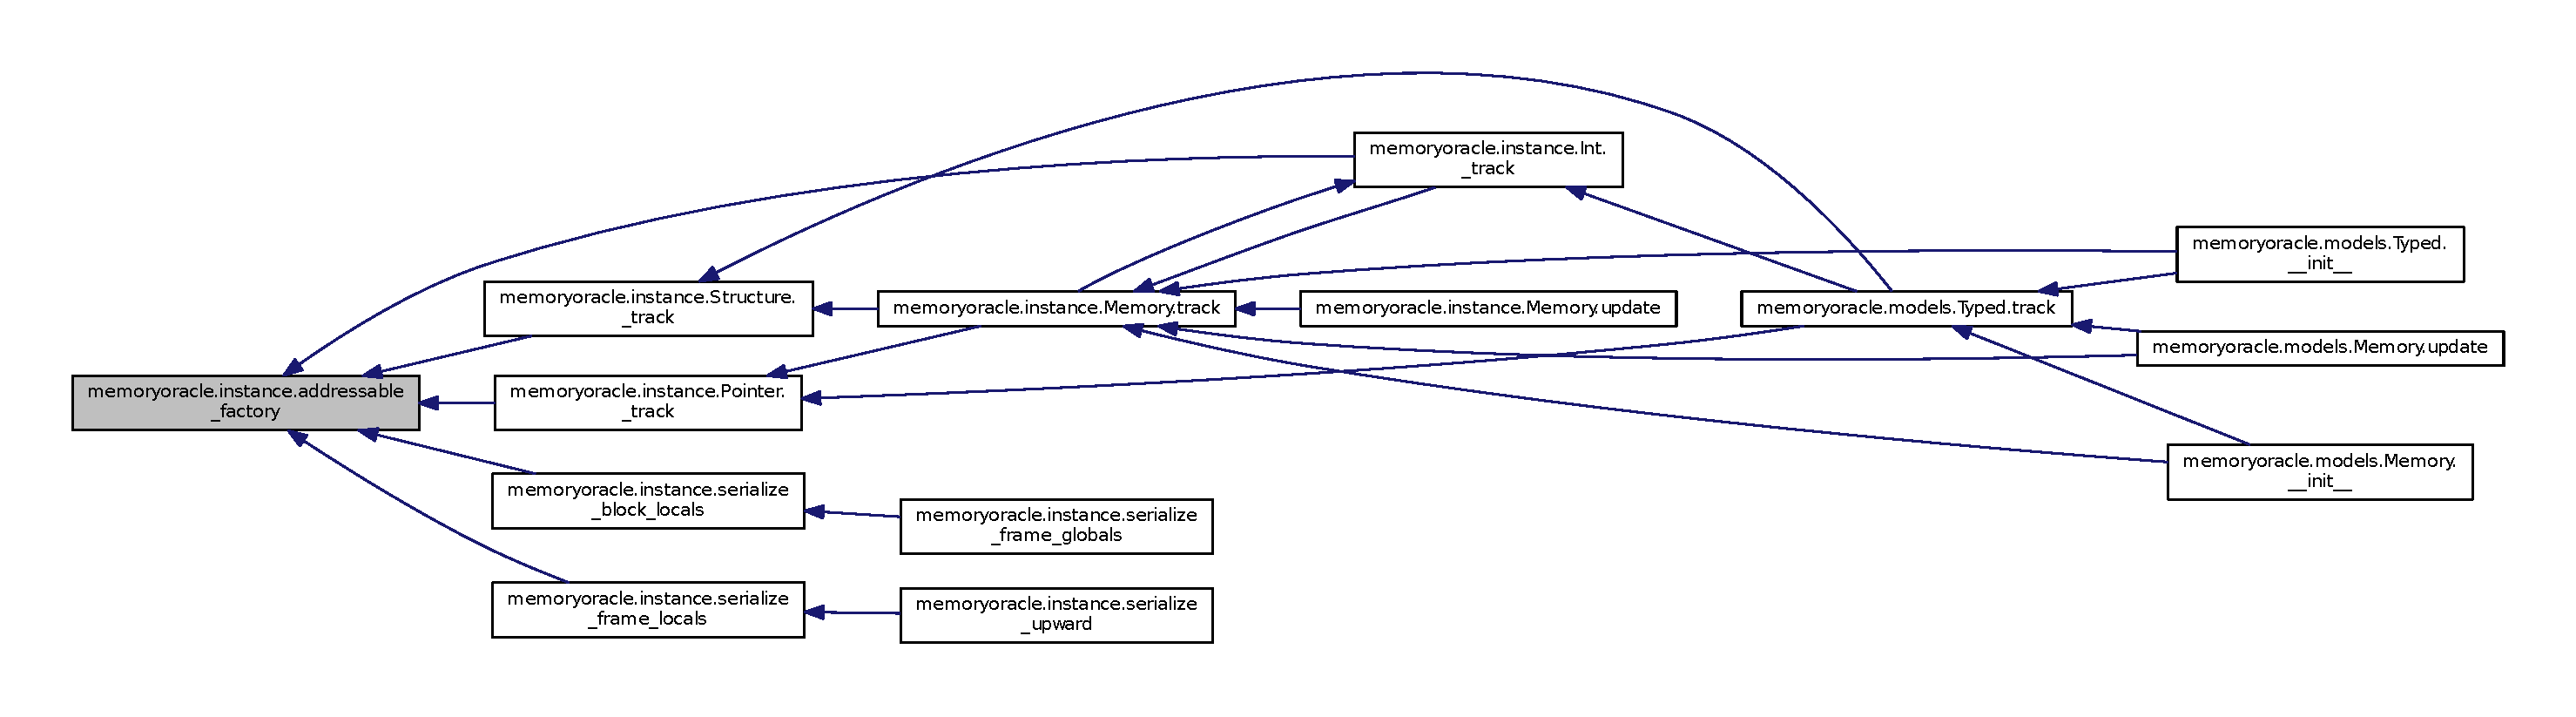
\includegraphics[width=350pt]{namespacememoryoracle_1_1instance_ac651a8635b1ae2ee7e788bf9adb17a0b_icgraph}
\end{center}
\end{figure}


\hypertarget{namespacememoryoracle_1_1instance_a31e7e3135691ee03e847163a5b1e3950}{}\index{memoryoracle\+::instance@{memoryoracle\+::instance}!get\+\_\+frame\+\_\+symbols@{get\+\_\+frame\+\_\+symbols}}
\index{get\+\_\+frame\+\_\+symbols@{get\+\_\+frame\+\_\+symbols}!memoryoracle\+::instance@{memoryoracle\+::instance}}
\subsubsection[{get\+\_\+frame\+\_\+symbols}]{\setlength{\rightskip}{0pt plus 5cm}def memoryoracle.\+instance.\+get\+\_\+frame\+\_\+symbols (
\begin{DoxyParamCaption}
\item[{}]{frm = {\ttfamily None}}
\end{DoxyParamCaption}
)}\label{namespacememoryoracle_1_1instance_a31e7e3135691ee03e847163a5b1e3950}


Definition at line 533 of file instance.\+py.



Referenced by memoryoracle.\+instance.\+serialize\+\_\+frame\+\_\+locals().


\begin{DoxyCode}
533 \textcolor{keyword}{def }\hyperlink{namespacememoryoracle_1_1instance_a31e7e3135691ee03e847163a5b1e3950}{get\_frame\_symbols}(frm=None):
534     with \hyperlink{classmemoryoracle_1_1frame_1_1Selector}{frame.Selector}(frm) \textcolor{keyword}{as} fs:
535         f = fs.frame
536         \textcolor{keywordflow}{if} f.is\_valid():
537             \textcolor{keywordflow}{return} \{ str(sym) \textcolor{keywordflow}{for} sym \textcolor{keywordflow}{in} f.block() \}
538         \textcolor{keywordflow}{else}:
539             \textcolor{keywordflow}{raise} Exception(\textcolor{stringliteral}{"Frame no longer valid"})
540 
\end{DoxyCode}


Here is the caller graph for this function\+:\nopagebreak
\begin{figure}[H]
\begin{center}
\leavevmode
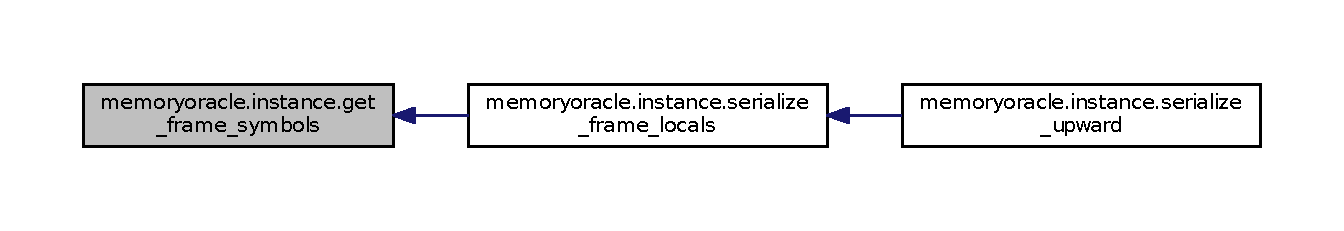
\includegraphics[width=350pt]{namespacememoryoracle_1_1instance_a31e7e3135691ee03e847163a5b1e3950_icgraph}
\end{center}
\end{figure}


\hypertarget{namespacememoryoracle_1_1instance_a78622e017f520b55ef2a05cffded052b}{}\index{memoryoracle\+::instance@{memoryoracle\+::instance}!serialize\+\_\+block\+\_\+locals@{serialize\+\_\+block\+\_\+locals}}
\index{serialize\+\_\+block\+\_\+locals@{serialize\+\_\+block\+\_\+locals}!memoryoracle\+::instance@{memoryoracle\+::instance}}
\subsubsection[{serialize\+\_\+block\+\_\+locals}]{\setlength{\rightskip}{0pt plus 5cm}def memoryoracle.\+instance.\+serialize\+\_\+block\+\_\+locals (
\begin{DoxyParamCaption}
\item[{}]{blk = {\ttfamily None}}
\end{DoxyParamCaption}
)}\label{namespacememoryoracle_1_1instance_a78622e017f520b55ef2a05cffded052b}


Definition at line 554 of file instance.\+py.



References memoryoracle.\+instance.\+addressable\+\_\+factory().



Referenced by memoryoracle.\+instance.\+serialize\+\_\+frame\+\_\+globals().


\begin{DoxyCode}
554 \textcolor{keyword}{def }\hyperlink{namespacememoryoracle_1_1instance_a78622e017f520b55ef2a05cffded052b}{serialize\_block\_locals}(blk = None):
555     Memory.\_updatedNames.clear()
556     block = blk \textcolor{keywordflow}{if} blk \textcolor{keywordflow}{is} \textcolor{keywordflow}{not} \textcolor{keywordtype}{None} \textcolor{keywordflow}{else} gdb.selected\_frame().block()
557     \textcolor{keywordflow}{for} sym \textcolor{keywordflow}{in} block:
558         \textcolor{keywordflow}{if} sym.is\_constant:
559             \textcolor{keywordflow}{continue}
560         desc = \hyperlink{classmemoryoracle_1_1descriptions_1_1MemoryDescription}{descriptions.MemoryDescription}(sym.name, symbol = sym)
561         \textcolor{keywordflow}{if} isinstance(desc.object, gdb.Symbol):
562             \textcolor{keywordflow}{continue}
563         obj = \hyperlink{namespacememoryoracle_1_1instance_ac651a8635b1ae2ee7e788bf9adb17a0b}{addressable\_factory}(desc)
564         obj.track()
565 
\end{DoxyCode}


Here is the call graph for this function\+:\nopagebreak
\begin{figure}[H]
\begin{center}
\leavevmode
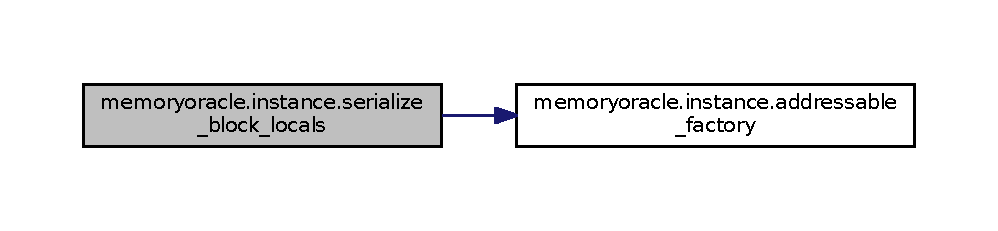
\includegraphics[width=350pt]{namespacememoryoracle_1_1instance_a78622e017f520b55ef2a05cffded052b_cgraph}
\end{center}
\end{figure}




Here is the caller graph for this function\+:\nopagebreak
\begin{figure}[H]
\begin{center}
\leavevmode
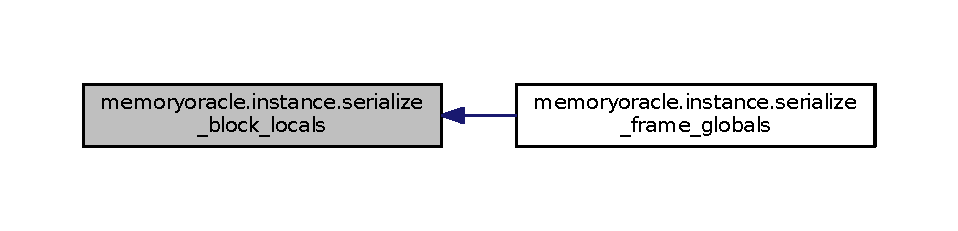
\includegraphics[width=350pt]{namespacememoryoracle_1_1instance_a78622e017f520b55ef2a05cffded052b_icgraph}
\end{center}
\end{figure}


\hypertarget{namespacememoryoracle_1_1instance_a2b902e26969fe19c09ad673fd8f1bbb5}{}\index{memoryoracle\+::instance@{memoryoracle\+::instance}!serialize\+\_\+frame\+\_\+globals@{serialize\+\_\+frame\+\_\+globals}}
\index{serialize\+\_\+frame\+\_\+globals@{serialize\+\_\+frame\+\_\+globals}!memoryoracle\+::instance@{memoryoracle\+::instance}}
\subsubsection[{serialize\+\_\+frame\+\_\+globals}]{\setlength{\rightskip}{0pt plus 5cm}def memoryoracle.\+instance.\+serialize\+\_\+frame\+\_\+globals (
\begin{DoxyParamCaption}
\item[{}]{frm = {\ttfamily None}}
\end{DoxyParamCaption}
)}\label{namespacememoryoracle_1_1instance_a2b902e26969fe19c09ad673fd8f1bbb5}


Definition at line 541 of file instance.\+py.



References memoryoracle.\+instance.\+serialize\+\_\+block\+\_\+locals().


\begin{DoxyCode}
541 \textcolor{keyword}{def }\hyperlink{namespacememoryoracle_1_1instance_a2b902e26969fe19c09ad673fd8f1bbb5}{serialize\_frame\_globals}(frm=None):
542     frame = frm \textcolor{keywordflow}{if} frm \textcolor{keywordflow}{is} \textcolor{keywordflow}{not} \textcolor{keywordtype}{None} \textcolor{keywordflow}{else} gdb.selected\_frame()
543     block = frame.block().global\_block
544     \hyperlink{namespacememoryoracle_1_1instance_a78622e017f520b55ef2a05cffded052b}{serialize\_block\_locals}(block)
545 
\end{DoxyCode}


Here is the call graph for this function\+:\nopagebreak
\begin{figure}[H]
\begin{center}
\leavevmode
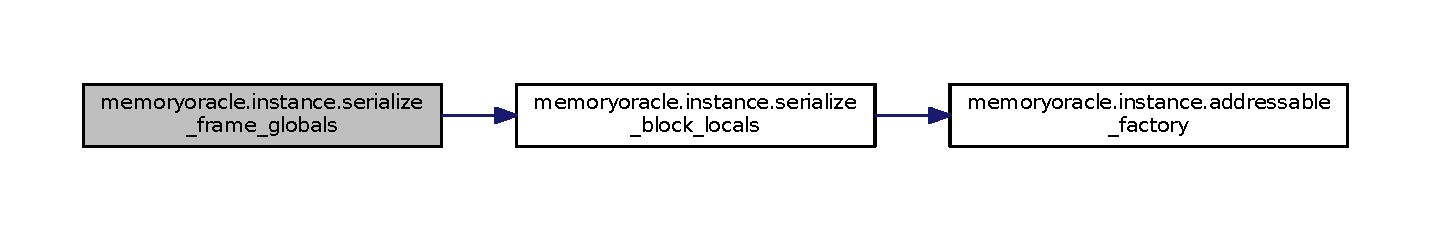
\includegraphics[width=350pt]{namespacememoryoracle_1_1instance_a2b902e26969fe19c09ad673fd8f1bbb5_cgraph}
\end{center}
\end{figure}


\hypertarget{namespacememoryoracle_1_1instance_a958b2f6afa09c327a9e48bbe2fc7f125}{}\index{memoryoracle\+::instance@{memoryoracle\+::instance}!serialize\+\_\+frame\+\_\+locals@{serialize\+\_\+frame\+\_\+locals}}
\index{serialize\+\_\+frame\+\_\+locals@{serialize\+\_\+frame\+\_\+locals}!memoryoracle\+::instance@{memoryoracle\+::instance}}
\subsubsection[{serialize\+\_\+frame\+\_\+locals}]{\setlength{\rightskip}{0pt plus 5cm}def memoryoracle.\+instance.\+serialize\+\_\+frame\+\_\+locals (
\begin{DoxyParamCaption}
\item[{}]{frm = {\ttfamily None}}
\end{DoxyParamCaption}
)}\label{namespacememoryoracle_1_1instance_a958b2f6afa09c327a9e48bbe2fc7f125}


Definition at line 566 of file instance.\+py.



References memoryoracle.\+instance.\+addressable\+\_\+factory(), and memoryoracle.\+instance.\+get\+\_\+frame\+\_\+symbols().



Referenced by memoryoracle.\+instance.\+serialize\+\_\+upward().


\begin{DoxyCode}
566 \textcolor{keyword}{def }\hyperlink{namespacememoryoracle_1_1instance_a958b2f6afa09c327a9e48bbe2fc7f125}{serialize\_frame\_locals}(frm = None):
567     Memory.\_updatedNames.clear()
568     \textcolor{keywordflow}{for} k \textcolor{keywordflow}{in} \hyperlink{namespacememoryoracle_1_1instance_a31e7e3135691ee03e847163a5b1e3950}{get\_frame\_symbols}(frm = frm):
569         desc = \hyperlink{classmemoryoracle_1_1descriptions_1_1MemoryDescription}{descriptions.MemoryDescription}(k)
570         obj = \hyperlink{namespacememoryoracle_1_1instance_ac651a8635b1ae2ee7e788bf9adb17a0b}{addressable\_factory}(desc)
571         obj.track()
572 
573 \textcolor{comment}{# def type\_name(t, nameDecorators = ""):}
574 \textcolor{comment}{#     if t.code == gdb.TYPE\_CODE\_PTR:}
575 \textcolor{comment}{#         return type\_name(t.target(), nameDecorators + "*")}
576 \textcolor{comment}{#     elif t.code == gdb.TYPE\_CODE\_ARRAY:}
577 \textcolor{comment}{#         length = str(t.range()[1] - t.range()[0] + 1)}
578 \textcolor{comment}{#         return type\_name(t.target(), nameDecorators + "[" + length + "]")}
579 \textcolor{comment}{#     else:}
580 \textcolor{comment}{#         return t.name + nameDecorators}
581 
\end{DoxyCode}


Here is the call graph for this function\+:\nopagebreak
\begin{figure}[H]
\begin{center}
\leavevmode
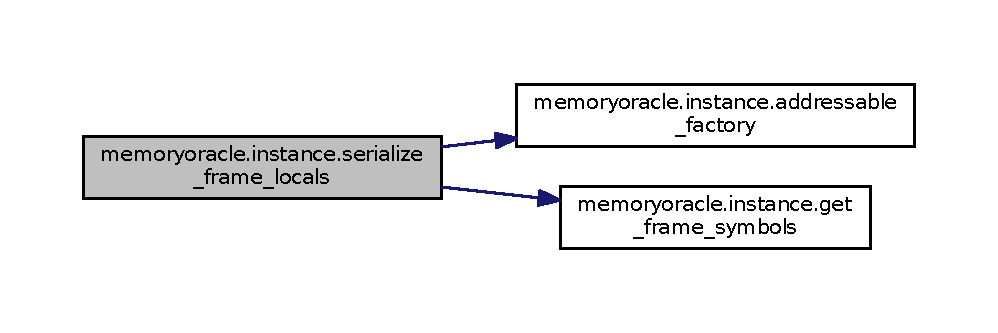
\includegraphics[width=350pt]{namespacememoryoracle_1_1instance_a958b2f6afa09c327a9e48bbe2fc7f125_cgraph}
\end{center}
\end{figure}




Here is the caller graph for this function\+:\nopagebreak
\begin{figure}[H]
\begin{center}
\leavevmode
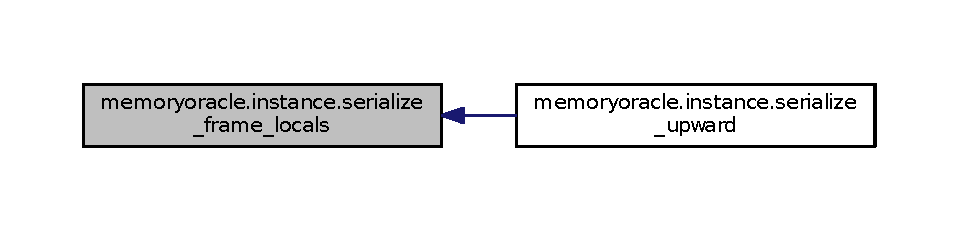
\includegraphics[width=350pt]{namespacememoryoracle_1_1instance_a958b2f6afa09c327a9e48bbe2fc7f125_icgraph}
\end{center}
\end{figure}


\hypertarget{namespacememoryoracle_1_1instance_a90a3c2f070ac8af0b41e6947d2b71a8a}{}\index{memoryoracle\+::instance@{memoryoracle\+::instance}!serialize\+\_\+upward@{serialize\+\_\+upward}}
\index{serialize\+\_\+upward@{serialize\+\_\+upward}!memoryoracle\+::instance@{memoryoracle\+::instance}}
\subsubsection[{serialize\+\_\+upward}]{\setlength{\rightskip}{0pt plus 5cm}def memoryoracle.\+instance.\+serialize\+\_\+upward (
\begin{DoxyParamCaption}
\item[{}]{base\+Block = {\ttfamily None}}
\end{DoxyParamCaption}
)}\label{namespacememoryoracle_1_1instance_a90a3c2f070ac8af0b41e6947d2b71a8a}


Definition at line 546 of file instance.\+py.



References memoryoracle.\+instance.\+serialize\+\_\+frame\+\_\+locals().


\begin{DoxyCode}
546 \textcolor{keyword}{def }\hyperlink{namespacememoryoracle_1_1instance_a90a3c2f070ac8af0b41e6947d2b71a8a}{serialize\_upward}(baseBlock = None):
547     \textcolor{keywordflow}{if} baseBlock \textcolor{keywordflow}{is} \textcolor{keywordtype}{None}:
548         f = gdb.newest\_frame()
549 
550     \textcolor{keywordflow}{while} f \textcolor{keywordflow}{is} \textcolor{keywordflow}{not} \textcolor{keywordtype}{None}:
551         \hyperlink{namespacememoryoracle_1_1instance_a958b2f6afa09c327a9e48bbe2fc7f125}{serialize\_frame\_locals}(f)
552         f = f.older()
553 
\end{DoxyCode}


Here is the call graph for this function\+:\nopagebreak
\begin{figure}[H]
\begin{center}
\leavevmode
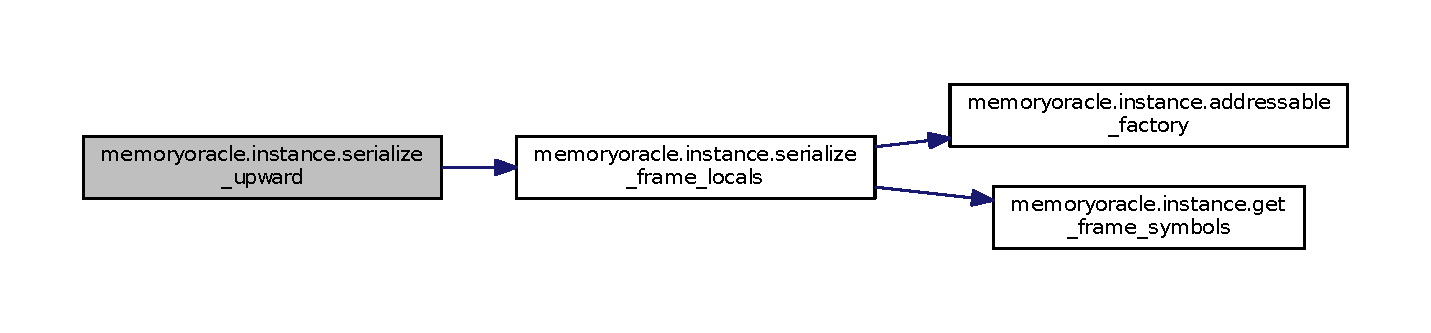
\includegraphics[width=350pt]{namespacememoryoracle_1_1instance_a90a3c2f070ac8af0b41e6947d2b71a8a_cgraph}
\end{center}
\end{figure}


\hypertarget{namespacememoryoracle_1_1instance_a05aa9c531f257d44ef9ac5f60f4e3859}{}\index{memoryoracle\+::instance@{memoryoracle\+::instance}!stopped@{stopped}}
\index{stopped@{stopped}!memoryoracle\+::instance@{memoryoracle\+::instance}}
\subsubsection[{stopped}]{\setlength{\rightskip}{0pt plus 5cm}def memoryoracle.\+instance.\+stopped (
\begin{DoxyParamCaption}
\item[{}]{event}
\end{DoxyParamCaption}
)}\label{namespacememoryoracle_1_1instance_a05aa9c531f257d44ef9ac5f60f4e3859}


Definition at line 594 of file instance.\+py.


\begin{DoxyCode}
594 \textcolor{keyword}{def }\hyperlink{namespacememoryoracle_1_1instance_a05aa9c531f257d44ef9ac5f60f4e3859}{stopped}(event):
595     arrayData = [ v2 \textcolor{keywordflow}{for} k, v \textcolor{keywordflow}{in} Array.repository.items() \textcolor{keywordflow}{for} k2, v2 \textcolor{keywordflow}{in} v.items() ]
596 
597     with open(\textcolor{stringliteral}{"arrays.json"}, \textcolor{stringliteral}{"w"}) \textcolor{keyword}{as} outfile:
598         json.dump(arrayData, outfile, cls=StateSerializer)
599 
600     with open(\textcolor{stringliteral}{"pointers.json"}, \textcolor{stringliteral}{"w"}) \textcolor{keyword}{as} outfile:
601         json.dump(Pointer.repository, outfile, cls=StateSerializer)
602 
603     with open(\textcolor{stringliteral}{"structs.json"}, \textcolor{stringliteral}{"w"}) \textcolor{keyword}{as} outfile:
604         json.dump(Structure.repository, outfile, cls=StateSerializer)
605 
606     with open(\textcolor{stringliteral}{"values.json"}, \textcolor{stringliteral}{"w"}) \textcolor{keyword}{as} outfile:
607         json.dump(Int.repository, outfile, cls=StateSerializer)
608 
609     \textcolor{comment}{# with open("functions.json", "w") as outfile:}
610     \textcolor{comment}{#     json.dump(Call.repository, outfile, cls=StateSerializer)}
611 
612 gdb.events.stop.connect(stopped)
613 
\end{DoxyCode}
\hypertarget{namespacememoryoracle_1_1instance_a4b8eb263a612b709be51201fc0fa7b6c}{}\index{memoryoracle\+::instance@{memoryoracle\+::instance}!target\+\_\+type\+\_\+name@{target\+\_\+type\+\_\+name}}
\index{target\+\_\+type\+\_\+name@{target\+\_\+type\+\_\+name}!memoryoracle\+::instance@{memoryoracle\+::instance}}
\subsubsection[{target\+\_\+type\+\_\+name}]{\setlength{\rightskip}{0pt plus 5cm}def memoryoracle.\+instance.\+target\+\_\+type\+\_\+name (
\begin{DoxyParamCaption}
\item[{}]{t}
\end{DoxyParamCaption}
)}\label{namespacememoryoracle_1_1instance_a4b8eb263a612b709be51201fc0fa7b6c}


Definition at line 582 of file instance.\+py.


\begin{DoxyCode}
582 \textcolor{keyword}{def }\hyperlink{namespacememoryoracle_1_1instance_a4b8eb263a612b709be51201fc0fa7b6c}{target\_type\_name}(t):
583     \textcolor{keywordflow}{if} t.code == gdb.TYPE\_CODE\_PTR \textcolor{keywordflow}{or} t.code == gdb.TYPE\_CODE\_ARRAY:
584         \textcolor{keywordflow}{return} \hyperlink{namespacememoryoracle_1_1instance_a4b8eb263a612b709be51201fc0fa7b6c}{target\_type\_name}(t.target())
585     \textcolor{keywordflow}{return} t.name
586 
\end{DoxyCode}


\subsection{Variable Documentation}
\hypertarget{namespacememoryoracle_1_1instance_a5e1db5ce414b598e74fcabb1803e1eb0}{}\index{memoryoracle\+::instance@{memoryoracle\+::instance}!connection@{connection}}
\index{connection@{connection}!memoryoracle\+::instance@{memoryoracle\+::instance}}
\subsubsection[{connection}]{\setlength{\rightskip}{0pt plus 5cm}tuple memoryoracle.\+instance.\+connection}\label{namespacememoryoracle_1_1instance_a5e1db5ce414b598e74fcabb1803e1eb0}
{\bfseries Initial value\+:}
\begin{DoxyCode}
1 = mongoengine.connect(\textcolor{stringliteral}{'memoryoracle'},
2                     read\_preference=\(\backslash\)
3                             pymongo.read\_preferences.ReadPreference.PRIMARY)
\end{DoxyCode}


Definition at line 28 of file instance.\+py.

\hypertarget{namespacememoryoracle_1_1instance_a50bbc043ba350bab4859e973b833b71f}{}\index{memoryoracle\+::instance@{memoryoracle\+::instance}!d@{d}}
\index{d@{d}!memoryoracle\+::instance@{memoryoracle\+::instance}}
\subsubsection[{d}]{\setlength{\rightskip}{0pt plus 5cm}tuple memoryoracle.\+instance.\+d = {\bf descriptions.\+Memory\+Description}(\char`\"{}a\char`\"{}, address=\char`\"{}1\char`\"{}, execution={\bf e})}\label{namespacememoryoracle_1_1instance_a50bbc043ba350bab4859e973b833b71f}


Definition at line 618 of file instance.\+py.

\hypertarget{namespacememoryoracle_1_1instance_ad0b99030c18c65a87129ed0c8a7d3b2e}{}\index{memoryoracle\+::instance@{memoryoracle\+::instance}!db@{db}}
\index{db@{db}!memoryoracle\+::instance@{memoryoracle\+::instance}}
\subsubsection[{db}]{\setlength{\rightskip}{0pt plus 5cm}memoryoracle.\+instance.\+db = connection.\+memoryoracle}\label{namespacememoryoracle_1_1instance_ad0b99030c18c65a87129ed0c8a7d3b2e}


Definition at line 32 of file instance.\+py.

\hypertarget{namespacememoryoracle_1_1instance_a8337088b8d0f8b6a58174f7b6a624d9e}{}\index{memoryoracle\+::instance@{memoryoracle\+::instance}!e@{e}}
\index{e@{e}!memoryoracle\+::instance@{memoryoracle\+::instance}}
\subsubsection[{e}]{\setlength{\rightskip}{0pt plus 5cm}tuple memoryoracle.\+instance.\+e = {\bf execution.\+Execution}()}\label{namespacememoryoracle_1_1instance_a8337088b8d0f8b6a58174f7b6a624d9e}


Definition at line 616 of file instance.\+py.

\hypertarget{namespacememoryoracle_1_1instance_a29d678ee2f2624880e57ee0ee498e793}{}\index{memoryoracle\+::instance@{memoryoracle\+::instance}!f@{f}}
\index{f@{f}!memoryoracle\+::instance@{memoryoracle\+::instance}}
\subsubsection[{f}]{\setlength{\rightskip}{0pt plus 5cm}tuple memoryoracle.\+instance.\+f = {\bf frame.\+Frame}(gdb.\+selected\+\_\+frame())}\label{namespacememoryoracle_1_1instance_a29d678ee2f2624880e57ee0ee498e793}


Definition at line 615 of file instance.\+py.

\hypertarget{namespacememoryoracle_1_1instance_ab71eabd3bbc314043bb5a1313cc3ab75}{}\index{memoryoracle\+::instance@{memoryoracle\+::instance}!frame\+Description@{frame\+Description}}
\index{frame\+Description@{frame\+Description}!memoryoracle\+::instance@{memoryoracle\+::instance}}
\subsubsection[{frame\+Description}]{\setlength{\rightskip}{0pt plus 5cm}tuple memoryoracle.\+instance.\+frame\+Description = {\bf descriptions.\+Memory\+Description}(\char`\"{}yourframe\char`\"{})}\label{namespacememoryoracle_1_1instance_ab71eabd3bbc314043bb5a1313cc3ab75}


Definition at line 614 of file instance.\+py.

\hypertarget{namespacememoryoracle_1_1instance_afe036cc8dc71469743d090c4c80d50c5}{}\index{memoryoracle\+::instance@{memoryoracle\+::instance}!x@{x}}
\index{x@{x}!memoryoracle\+::instance@{memoryoracle\+::instance}}
\subsubsection[{x}]{\setlength{\rightskip}{0pt plus 5cm}tuple memoryoracle.\+instance.\+x = {\bf Float.\+factory}(descript={\bf d})}\label{namespacememoryoracle_1_1instance_afe036cc8dc71469743d090c4c80d50c5}


Definition at line 619 of file instance.\+py.



Referenced by memoryoracle.\+test\+\_\+models.\+Program\+Test\+Data.\+set\+\_\+up\+\_\+class(), memoryoracle.\+test\+\_\+models.\+Commit\+Test\+Data.\+set\+\_\+up\+\_\+class(), memoryoracle.\+test\+\_\+models.\+Executable\+Test\+Data.\+set\+\_\+up\+\_\+class(), memoryoracle.\+test\+\_\+models.\+Execution\+Test\+Data.\+set\+\_\+up\+\_\+class(), memoryoracle.\+test\+\_\+models.\+Memory\+Test\+Data.\+set\+\_\+up\+\_\+class(), memoryoracle.\+test\+\_\+models.\+Object\+File\+Test\+Data.\+set\+\_\+up\+\_\+class(), memoryoracle.\+test\+\_\+models.\+Source\+File\+Test\+Data.\+set\+\_\+up\+\_\+class(), and memoryoracle.\+test\+\_\+models.\+Symbol\+Test\+Data.\+set\+\_\+up\+\_\+class().


\hypertarget{namespacememoryoracle_1_1migrations}{}\section{memoryoracle.\+migrations Namespace Reference}
\label{namespacememoryoracle_1_1migrations}\index{memoryoracle.\+migrations@{memoryoracle.\+migrations}}
\subsection*{Namespaces}
\begin{DoxyCompactItemize}
\item 
 \hyperlink{namespacememoryoracle_1_1migrations_1_10001__initial}{0001\+\_\+initial}
\item 
 \hyperlink{namespacememoryoracle_1_1migrations_1_10002__auto__20150402__2000}{0002\+\_\+auto\+\_\+20150402\+\_\+2000}
\item 
 \hyperlink{namespacememoryoracle_1_1migrations_1_10003__auto__20150402__2000}{0003\+\_\+auto\+\_\+20150402\+\_\+2000}
\item 
 \hyperlink{namespacememoryoracle_1_1migrations_1_10004__auto__20150402__2000}{0004\+\_\+auto\+\_\+20150402\+\_\+2000}
\item 
 \hyperlink{namespacememoryoracle_1_1migrations_1_10005__auto__20150403__0100}{0005\+\_\+auto\+\_\+20150403\+\_\+0100}
\item 
 \hyperlink{namespacememoryoracle_1_1migrations_1_10006__program__path}{0006\+\_\+program\+\_\+path}
\item 
 \hyperlink{namespacememoryoracle_1_1migrations_1_10007__auto__20150403__0248}{0007\+\_\+auto\+\_\+20150403\+\_\+0248}
\end{DoxyCompactItemize}

\hypertarget{namespacememoryoracle_1_1migrations_1_10001__initial}{}\section{memoryoracle.\+migrations.0001\+\_\+initial Namespace Reference}
\label{namespacememoryoracle_1_1migrations_1_10001__initial}\index{memoryoracle.\+migrations.\+0001\+\_\+initial@{memoryoracle.\+migrations.\+0001\+\_\+initial}}
\subsection*{Classes}
\begin{DoxyCompactItemize}
\item 
class \hyperlink{classmemoryoracle_1_1migrations_1_10001__initial_1_1Migration}{Migration}
\end{DoxyCompactItemize}

\hypertarget{namespacememoryoracle_1_1migrations_1_10002__auto__20150402__2000}{}\section{memoryoracle.\+migrations.0002\+\_\+auto\+\_\+20150402\+\_\+2000 Namespace Reference}
\label{namespacememoryoracle_1_1migrations_1_10002__auto__20150402__2000}\index{memoryoracle.\+migrations.\+0002\+\_\+auto\+\_\+20150402\+\_\+2000@{memoryoracle.\+migrations.\+0002\+\_\+auto\+\_\+20150402\+\_\+2000}}
\subsection*{Classes}
\begin{DoxyCompactItemize}
\item 
class \hyperlink{classmemoryoracle_1_1migrations_1_10002__auto__20150402__2000_1_1Migration}{Migration}
\end{DoxyCompactItemize}

\hypertarget{namespacememoryoracle_1_1migrations_1_10003__auto__20150402__2000}{}\section{memoryoracle.\+migrations.0003\+\_\+auto\+\_\+20150402\+\_\+2000 Namespace Reference}
\label{namespacememoryoracle_1_1migrations_1_10003__auto__20150402__2000}\index{memoryoracle.\+migrations.\+0003\+\_\+auto\+\_\+20150402\+\_\+2000@{memoryoracle.\+migrations.\+0003\+\_\+auto\+\_\+20150402\+\_\+2000}}
\subsection*{Classes}
\begin{DoxyCompactItemize}
\item 
class \hyperlink{classmemoryoracle_1_1migrations_1_10003__auto__20150402__2000_1_1Migration}{Migration}
\end{DoxyCompactItemize}

\hypertarget{namespacememoryoracle_1_1migrations_1_10004__auto__20150402__2000}{}\section{memoryoracle.\+migrations.0004\+\_\+auto\+\_\+20150402\+\_\+2000 Namespace Reference}
\label{namespacememoryoracle_1_1migrations_1_10004__auto__20150402__2000}\index{memoryoracle.\+migrations.\+0004\+\_\+auto\+\_\+20150402\+\_\+2000@{memoryoracle.\+migrations.\+0004\+\_\+auto\+\_\+20150402\+\_\+2000}}
\subsection*{Classes}
\begin{DoxyCompactItemize}
\item 
class \hyperlink{classmemoryoracle_1_1migrations_1_10004__auto__20150402__2000_1_1Migration}{Migration}
\end{DoxyCompactItemize}

\hypertarget{namespacememoryoracle_1_1migrations_1_10005__auto__20150403__0100}{}\section{memoryoracle.\+migrations.0005\+\_\+auto\+\_\+20150403\+\_\+0100 Namespace Reference}
\label{namespacememoryoracle_1_1migrations_1_10005__auto__20150403__0100}\index{memoryoracle.\+migrations.\+0005\+\_\+auto\+\_\+20150403\+\_\+0100@{memoryoracle.\+migrations.\+0005\+\_\+auto\+\_\+20150403\+\_\+0100}}
\subsection*{Classes}
\begin{DoxyCompactItemize}
\item 
class \hyperlink{classmemoryoracle_1_1migrations_1_10005__auto__20150403__0100_1_1Migration}{Migration}
\end{DoxyCompactItemize}

\hypertarget{namespacememoryoracle_1_1migrations_1_10006__program__path}{}\section{memoryoracle.\+migrations.0006\+\_\+program\+\_\+path Namespace Reference}
\label{namespacememoryoracle_1_1migrations_1_10006__program__path}\index{memoryoracle.\+migrations.\+0006\+\_\+program\+\_\+path@{memoryoracle.\+migrations.\+0006\+\_\+program\+\_\+path}}
\subsection*{Classes}
\begin{DoxyCompactItemize}
\item 
class \hyperlink{classmemoryoracle_1_1migrations_1_10006__program__path_1_1Migration}{Migration}
\end{DoxyCompactItemize}

\hypertarget{namespacememoryoracle_1_1migrations_1_10007__auto__20150403__0248}{}\section{memoryoracle.\+migrations.0007\+\_\+auto\+\_\+20150403\+\_\+0248 Namespace Reference}
\label{namespacememoryoracle_1_1migrations_1_10007__auto__20150403__0248}\index{memoryoracle.\+migrations.\+0007\+\_\+auto\+\_\+20150403\+\_\+0248@{memoryoracle.\+migrations.\+0007\+\_\+auto\+\_\+20150403\+\_\+0248}}
\subsection*{Classes}
\begin{DoxyCompactItemize}
\item 
class \hyperlink{classmemoryoracle_1_1migrations_1_10007__auto__20150403__0248_1_1Migration}{Migration}
\end{DoxyCompactItemize}

\hypertarget{namespacememoryoracle_1_1models}{}\section{memoryoracle.\+models Namespace Reference}
\label{namespacememoryoracle_1_1models}\index{memoryoracle.\+models@{memoryoracle.\+models}}
\subsection*{Classes}
\begin{DoxyCompactItemize}
\item 
class \hyperlink{classmemoryoracle_1_1models_1_1Commit}{Commit}
\item 
class \hyperlink{classmemoryoracle_1_1models_1_1Executable}{Executable}
\item 
class \hyperlink{classmemoryoracle_1_1models_1_1Execution}{Execution}
\item 
class \hyperlink{classmemoryoracle_1_1models_1_1Memory}{Memory}
\item 
class \hyperlink{classmemoryoracle_1_1models_1_1ObjectFile}{Object\+File}
\item 
class \hyperlink{classmemoryoracle_1_1models_1_1Program}{Program}
\item 
class \hyperlink{classmemoryoracle_1_1models_1_1ProgramFile}{Program\+File}
\item 
class \hyperlink{classmemoryoracle_1_1models_1_1Schema}{Schema}
\item 
class \hyperlink{classmemoryoracle_1_1models_1_1SourceFile}{Source\+File}
\item 
class \hyperlink{classmemoryoracle_1_1models_1_1Symbol}{Symbol}
\item 
class \hyperlink{classmemoryoracle_1_1models_1_1Tracked}{Tracked}
\item 
class \hyperlink{classmemoryoracle_1_1models_1_1Type}{Type}
\item 
class \hyperlink{classmemoryoracle_1_1models_1_1Typed}{Typed}
\end{DoxyCompactItemize}

\hypertarget{namespacememoryoracle_1_1registry}{}\section{memoryoracle.\+registry Namespace Reference}
\label{namespacememoryoracle_1_1registry}\index{memoryoracle.\+registry@{memoryoracle.\+registry}}
\subsection*{Classes}
\begin{DoxyCompactItemize}
\item 
class \hyperlink{classmemoryoracle_1_1registry_1_1TypeDetectionError}{Type\+Detection\+Error}
\item 
class \hyperlink{classmemoryoracle_1_1registry_1_1TypeRegistration}{Type\+Registration}
\end{DoxyCompactItemize}

\hypertarget{namespacememoryoracle_1_1settings}{}\section{memoryoracle.\+settings Namespace Reference}
\label{namespacememoryoracle_1_1settings}\index{memoryoracle.\+settings@{memoryoracle.\+settings}}
\subsection*{Variables}
\begin{DoxyCompactItemize}
\item 
tuple \hyperlink{namespacememoryoracle_1_1settings_a863b63594639ca54681c195b58eb1b27}{B\+A\+S\+E\+\_\+\+D\+I\+R} = os.\+path.\+dirname(os.\+path.\+dirname(\+\_\+\+\_\+file\+\_\+\+\_\+))
\item 
string \hyperlink{namespacememoryoracle_1_1settings_a8a181b7a3e7e47b16b6900941d5d6284}{S\+E\+C\+R\+E\+T\+\_\+\+K\+E\+Y} = \textquotesingle{}w=6vi9p\+\_\+z8ik\%0(843=zmjv$\ast$\$5qc\$kf\+\_\+g!lo5-\/vqy1nd+e368b\textquotesingle{}
\item 
\hyperlink{namespacememoryoracle_1_1settings_a27514ec5b2f50b45fc52ed1ce0bed93a}{D\+E\+B\+U\+G} = True
\item 
\hyperlink{namespacememoryoracle_1_1settings_adb6dc4ebf65e09f416038d725c2ddec4}{T\+E\+M\+P\+L\+A\+T\+E\+\_\+\+D\+E\+B\+U\+G} = True
\item 
list \hyperlink{namespacememoryoracle_1_1settings_ad8ebc3cca1f2eb2beaab000158d3a26c}{A\+L\+L\+O\+W\+E\+D\+\_\+\+H\+O\+S\+T\+S} = \mbox{[}$\,$\mbox{]}
\item 
tuple \hyperlink{namespacememoryoracle_1_1settings_aa30625d00c355a4e99113af5732a1b76}{I\+N\+S\+T\+A\+L\+L\+E\+D\+\_\+\+A\+P\+P\+S}
\item 
tuple \hyperlink{namespacememoryoracle_1_1settings_a22348e05f0743ec99f37a8cf94154efc}{M\+I\+D\+D\+L\+E\+W\+A\+R\+E\+\_\+\+C\+L\+A\+S\+S\+E\+S}
\item 
string \hyperlink{namespacememoryoracle_1_1settings_a6c9ce7dd487f150eeac964208a5cdec6}{R\+O\+O\+T\+\_\+\+U\+R\+L\+C\+O\+N\+F} = \textquotesingle{}memoryoracle.\+urls\textquotesingle{}
\item 
string \hyperlink{namespacememoryoracle_1_1settings_ad4789b93d4ce7e968b078d08624ec529}{W\+S\+G\+I\+\_\+\+A\+P\+P\+L\+I\+C\+A\+T\+I\+O\+N} = \textquotesingle{}\hyperlink{namespacememoryoracle_1_1wsgi_aa19120d9c42407746c9676a96206f976}{memoryoracle.\+wsgi.\+application}\textquotesingle{}
\item 
dictionary \hyperlink{namespacememoryoracle_1_1settings_acb2be5a1881ee462bf8301b2e47754f4}{D\+A\+T\+A\+B\+A\+S\+E\+S}
\item 
string \hyperlink{namespacememoryoracle_1_1settings_aa38fcebeba95ab0de566b589068a6aea}{L\+A\+N\+G\+U\+A\+G\+E\+\_\+\+C\+O\+D\+E} = \textquotesingle{}en-\/us\textquotesingle{}
\item 
string \hyperlink{namespacememoryoracle_1_1settings_a71b87e5d3e6de18ad0701a27d643558a}{T\+I\+M\+E\+\_\+\+Z\+O\+N\+E} = \textquotesingle{}U\+T\+C\textquotesingle{}
\item 
\hyperlink{namespacememoryoracle_1_1settings_a8788c114be7d1e83fe9f03e1a9bc4f4d}{U\+S\+E\+\_\+\+I18\+N} = True
\item 
\hyperlink{namespacememoryoracle_1_1settings_a59082cdfd1b4c6cde674a08c04015557}{U\+S\+E\+\_\+\+L10\+N} = True
\item 
\hyperlink{namespacememoryoracle_1_1settings_a4fa7a9ff610d0fe7965cd9f795d99aca}{U\+S\+E\+\_\+\+T\+Z} = True
\item 
string \hyperlink{namespacememoryoracle_1_1settings_acb558760188386601f245688e233bcd8}{S\+T\+A\+T\+I\+C\+\_\+\+U\+R\+L} = \textquotesingle{}/static/\textquotesingle{}
\end{DoxyCompactItemize}


\subsection{Detailed Description}
\begin{DoxyVerb}Django settings for memoryoracle project.

For more information on this file, see
https://docs.djangoproject.com/en/1.7/topics/settings/

For the full list of settings and their values, see
https://docs.djangoproject.com/en/1.7/ref/settings/
\end{DoxyVerb}
 

\subsection{Variable Documentation}
\hypertarget{namespacememoryoracle_1_1settings_ad8ebc3cca1f2eb2beaab000158d3a26c}{}\index{memoryoracle\+::settings@{memoryoracle\+::settings}!A\+L\+L\+O\+W\+E\+D\+\_\+\+H\+O\+S\+T\+S@{A\+L\+L\+O\+W\+E\+D\+\_\+\+H\+O\+S\+T\+S}}
\index{A\+L\+L\+O\+W\+E\+D\+\_\+\+H\+O\+S\+T\+S@{A\+L\+L\+O\+W\+E\+D\+\_\+\+H\+O\+S\+T\+S}!memoryoracle\+::settings@{memoryoracle\+::settings}}
\subsubsection[{A\+L\+L\+O\+W\+E\+D\+\_\+\+H\+O\+S\+T\+S}]{\setlength{\rightskip}{0pt plus 5cm}list memoryoracle.\+settings.\+A\+L\+L\+O\+W\+E\+D\+\_\+\+H\+O\+S\+T\+S = \mbox{[}$\,$\mbox{]}}\label{namespacememoryoracle_1_1settings_ad8ebc3cca1f2eb2beaab000158d3a26c}


Definition at line 27 of file settings.\+py.

\hypertarget{namespacememoryoracle_1_1settings_a863b63594639ca54681c195b58eb1b27}{}\index{memoryoracle\+::settings@{memoryoracle\+::settings}!B\+A\+S\+E\+\_\+\+D\+I\+R@{B\+A\+S\+E\+\_\+\+D\+I\+R}}
\index{B\+A\+S\+E\+\_\+\+D\+I\+R@{B\+A\+S\+E\+\_\+\+D\+I\+R}!memoryoracle\+::settings@{memoryoracle\+::settings}}
\subsubsection[{B\+A\+S\+E\+\_\+\+D\+I\+R}]{\setlength{\rightskip}{0pt plus 5cm}tuple memoryoracle.\+settings.\+B\+A\+S\+E\+\_\+\+D\+I\+R = os.\+path.\+dirname(os.\+path.\+dirname(\+\_\+\+\_\+file\+\_\+\+\_\+))}\label{namespacememoryoracle_1_1settings_a863b63594639ca54681c195b58eb1b27}


Definition at line 13 of file settings.\+py.

\hypertarget{namespacememoryoracle_1_1settings_acb2be5a1881ee462bf8301b2e47754f4}{}\index{memoryoracle\+::settings@{memoryoracle\+::settings}!D\+A\+T\+A\+B\+A\+S\+E\+S@{D\+A\+T\+A\+B\+A\+S\+E\+S}}
\index{D\+A\+T\+A\+B\+A\+S\+E\+S@{D\+A\+T\+A\+B\+A\+S\+E\+S}!memoryoracle\+::settings@{memoryoracle\+::settings}}
\subsubsection[{D\+A\+T\+A\+B\+A\+S\+E\+S}]{\setlength{\rightskip}{0pt plus 5cm}dictionary memoryoracle.\+settings.\+D\+A\+T\+A\+B\+A\+S\+E\+S}\label{namespacememoryoracle_1_1settings_acb2be5a1881ee462bf8301b2e47754f4}
{\bfseries Initial value\+:}
\begin{DoxyCode}
1 = \{
2     \textcolor{stringliteral}{'default'}: \{
3         \textcolor{stringliteral}{'ENGINE'}: \textcolor{stringliteral}{'django\_mongodb\_engine'},
4         \textcolor{stringliteral}{'NAME'}: \textcolor{stringliteral}{'memoryoracle'}
5     \}
6 \}
\end{DoxyCode}


Definition at line 70 of file settings.\+py.

\hypertarget{namespacememoryoracle_1_1settings_a27514ec5b2f50b45fc52ed1ce0bed93a}{}\index{memoryoracle\+::settings@{memoryoracle\+::settings}!D\+E\+B\+U\+G@{D\+E\+B\+U\+G}}
\index{D\+E\+B\+U\+G@{D\+E\+B\+U\+G}!memoryoracle\+::settings@{memoryoracle\+::settings}}
\subsubsection[{D\+E\+B\+U\+G}]{\setlength{\rightskip}{0pt plus 5cm}memoryoracle.\+settings.\+D\+E\+B\+U\+G = True}\label{namespacememoryoracle_1_1settings_a27514ec5b2f50b45fc52ed1ce0bed93a}


Definition at line 23 of file settings.\+py.

\hypertarget{namespacememoryoracle_1_1settings_aa30625d00c355a4e99113af5732a1b76}{}\index{memoryoracle\+::settings@{memoryoracle\+::settings}!I\+N\+S\+T\+A\+L\+L\+E\+D\+\_\+\+A\+P\+P\+S@{I\+N\+S\+T\+A\+L\+L\+E\+D\+\_\+\+A\+P\+P\+S}}
\index{I\+N\+S\+T\+A\+L\+L\+E\+D\+\_\+\+A\+P\+P\+S@{I\+N\+S\+T\+A\+L\+L\+E\+D\+\_\+\+A\+P\+P\+S}!memoryoracle\+::settings@{memoryoracle\+::settings}}
\subsubsection[{I\+N\+S\+T\+A\+L\+L\+E\+D\+\_\+\+A\+P\+P\+S}]{\setlength{\rightskip}{0pt plus 5cm}tuple memoryoracle.\+settings.\+I\+N\+S\+T\+A\+L\+L\+E\+D\+\_\+\+A\+P\+P\+S}\label{namespacememoryoracle_1_1settings_aa30625d00c355a4e99113af5732a1b76}
{\bfseries Initial value\+:}
\begin{DoxyCode}
1 = (
2     \textcolor{stringliteral}{'django.contrib.admin'},
3     \textcolor{stringliteral}{'django.contrib.auth'},
4     \textcolor{stringliteral}{'django.contrib.contenttypes'},
5     \textcolor{stringliteral}{'django.contrib.sessions'},
6     \textcolor{stringliteral}{'django.contrib.messages'},
7     \textcolor{stringliteral}{'django.contrib.staticfiles'},
8     \textcolor{stringliteral}{'memoryoracle'},
9 )
\end{DoxyCode}


Definition at line 32 of file settings.\+py.

\hypertarget{namespacememoryoracle_1_1settings_aa38fcebeba95ab0de566b589068a6aea}{}\index{memoryoracle\+::settings@{memoryoracle\+::settings}!L\+A\+N\+G\+U\+A\+G\+E\+\_\+\+C\+O\+D\+E@{L\+A\+N\+G\+U\+A\+G\+E\+\_\+\+C\+O\+D\+E}}
\index{L\+A\+N\+G\+U\+A\+G\+E\+\_\+\+C\+O\+D\+E@{L\+A\+N\+G\+U\+A\+G\+E\+\_\+\+C\+O\+D\+E}!memoryoracle\+::settings@{memoryoracle\+::settings}}
\subsubsection[{L\+A\+N\+G\+U\+A\+G\+E\+\_\+\+C\+O\+D\+E}]{\setlength{\rightskip}{0pt plus 5cm}string memoryoracle.\+settings.\+L\+A\+N\+G\+U\+A\+G\+E\+\_\+\+C\+O\+D\+E = \textquotesingle{}en-\/us\textquotesingle{}}\label{namespacememoryoracle_1_1settings_aa38fcebeba95ab0de566b589068a6aea}


Definition at line 80 of file settings.\+py.

\hypertarget{namespacememoryoracle_1_1settings_a22348e05f0743ec99f37a8cf94154efc}{}\index{memoryoracle\+::settings@{memoryoracle\+::settings}!M\+I\+D\+D\+L\+E\+W\+A\+R\+E\+\_\+\+C\+L\+A\+S\+S\+E\+S@{M\+I\+D\+D\+L\+E\+W\+A\+R\+E\+\_\+\+C\+L\+A\+S\+S\+E\+S}}
\index{M\+I\+D\+D\+L\+E\+W\+A\+R\+E\+\_\+\+C\+L\+A\+S\+S\+E\+S@{M\+I\+D\+D\+L\+E\+W\+A\+R\+E\+\_\+\+C\+L\+A\+S\+S\+E\+S}!memoryoracle\+::settings@{memoryoracle\+::settings}}
\subsubsection[{M\+I\+D\+D\+L\+E\+W\+A\+R\+E\+\_\+\+C\+L\+A\+S\+S\+E\+S}]{\setlength{\rightskip}{0pt plus 5cm}tuple memoryoracle.\+settings.\+M\+I\+D\+D\+L\+E\+W\+A\+R\+E\+\_\+\+C\+L\+A\+S\+S\+E\+S}\label{namespacememoryoracle_1_1settings_a22348e05f0743ec99f37a8cf94154efc}
{\bfseries Initial value\+:}
\begin{DoxyCode}
1 = (
2     \textcolor{stringliteral}{'django.contrib.sessions.middleware.SessionMiddleware'},
3     \textcolor{stringliteral}{'django.middleware.common.CommonMiddleware'},
4     \textcolor{stringliteral}{'django.middleware.csrf.CsrfViewMiddleware'},
5     \textcolor{stringliteral}{'django.contrib.auth.middleware.AuthenticationMiddleware'},
6     \textcolor{stringliteral}{'django.contrib.auth.middleware.SessionAuthenticationMiddleware'},
7     \textcolor{stringliteral}{'django.contrib.messages.middleware.MessageMiddleware'},
8     \textcolor{stringliteral}{'django.middleware.clickjacking.XFrameOptionsMiddleware'},
9 )
\end{DoxyCode}


Definition at line 42 of file settings.\+py.

\hypertarget{namespacememoryoracle_1_1settings_a6c9ce7dd487f150eeac964208a5cdec6}{}\index{memoryoracle\+::settings@{memoryoracle\+::settings}!R\+O\+O\+T\+\_\+\+U\+R\+L\+C\+O\+N\+F@{R\+O\+O\+T\+\_\+\+U\+R\+L\+C\+O\+N\+F}}
\index{R\+O\+O\+T\+\_\+\+U\+R\+L\+C\+O\+N\+F@{R\+O\+O\+T\+\_\+\+U\+R\+L\+C\+O\+N\+F}!memoryoracle\+::settings@{memoryoracle\+::settings}}
\subsubsection[{R\+O\+O\+T\+\_\+\+U\+R\+L\+C\+O\+N\+F}]{\setlength{\rightskip}{0pt plus 5cm}string memoryoracle.\+settings.\+R\+O\+O\+T\+\_\+\+U\+R\+L\+C\+O\+N\+F = \textquotesingle{}memoryoracle.\+urls\textquotesingle{}}\label{namespacememoryoracle_1_1settings_a6c9ce7dd487f150eeac964208a5cdec6}


Definition at line 52 of file settings.\+py.

\hypertarget{namespacememoryoracle_1_1settings_a8a181b7a3e7e47b16b6900941d5d6284}{}\index{memoryoracle\+::settings@{memoryoracle\+::settings}!S\+E\+C\+R\+E\+T\+\_\+\+K\+E\+Y@{S\+E\+C\+R\+E\+T\+\_\+\+K\+E\+Y}}
\index{S\+E\+C\+R\+E\+T\+\_\+\+K\+E\+Y@{S\+E\+C\+R\+E\+T\+\_\+\+K\+E\+Y}!memoryoracle\+::settings@{memoryoracle\+::settings}}
\subsubsection[{S\+E\+C\+R\+E\+T\+\_\+\+K\+E\+Y}]{\setlength{\rightskip}{0pt plus 5cm}string memoryoracle.\+settings.\+S\+E\+C\+R\+E\+T\+\_\+\+K\+E\+Y = \textquotesingle{}w=6vi9p\+\_\+z8ik\%0(843=zmjv$\ast$\$5qc\$kf\+\_\+g!lo5-\/vqy1nd+e368b\textquotesingle{}}\label{namespacememoryoracle_1_1settings_a8a181b7a3e7e47b16b6900941d5d6284}


Definition at line 20 of file settings.\+py.

\hypertarget{namespacememoryoracle_1_1settings_acb558760188386601f245688e233bcd8}{}\index{memoryoracle\+::settings@{memoryoracle\+::settings}!S\+T\+A\+T\+I\+C\+\_\+\+U\+R\+L@{S\+T\+A\+T\+I\+C\+\_\+\+U\+R\+L}}
\index{S\+T\+A\+T\+I\+C\+\_\+\+U\+R\+L@{S\+T\+A\+T\+I\+C\+\_\+\+U\+R\+L}!memoryoracle\+::settings@{memoryoracle\+::settings}}
\subsubsection[{S\+T\+A\+T\+I\+C\+\_\+\+U\+R\+L}]{\setlength{\rightskip}{0pt plus 5cm}string memoryoracle.\+settings.\+S\+T\+A\+T\+I\+C\+\_\+\+U\+R\+L = \textquotesingle{}/static/\textquotesingle{}}\label{namespacememoryoracle_1_1settings_acb558760188386601f245688e233bcd8}


Definition at line 94 of file settings.\+py.

\hypertarget{namespacememoryoracle_1_1settings_adb6dc4ebf65e09f416038d725c2ddec4}{}\index{memoryoracle\+::settings@{memoryoracle\+::settings}!T\+E\+M\+P\+L\+A\+T\+E\+\_\+\+D\+E\+B\+U\+G@{T\+E\+M\+P\+L\+A\+T\+E\+\_\+\+D\+E\+B\+U\+G}}
\index{T\+E\+M\+P\+L\+A\+T\+E\+\_\+\+D\+E\+B\+U\+G@{T\+E\+M\+P\+L\+A\+T\+E\+\_\+\+D\+E\+B\+U\+G}!memoryoracle\+::settings@{memoryoracle\+::settings}}
\subsubsection[{T\+E\+M\+P\+L\+A\+T\+E\+\_\+\+D\+E\+B\+U\+G}]{\setlength{\rightskip}{0pt plus 5cm}memoryoracle.\+settings.\+T\+E\+M\+P\+L\+A\+T\+E\+\_\+\+D\+E\+B\+U\+G = True}\label{namespacememoryoracle_1_1settings_adb6dc4ebf65e09f416038d725c2ddec4}


Definition at line 25 of file settings.\+py.

\hypertarget{namespacememoryoracle_1_1settings_a71b87e5d3e6de18ad0701a27d643558a}{}\index{memoryoracle\+::settings@{memoryoracle\+::settings}!T\+I\+M\+E\+\_\+\+Z\+O\+N\+E@{T\+I\+M\+E\+\_\+\+Z\+O\+N\+E}}
\index{T\+I\+M\+E\+\_\+\+Z\+O\+N\+E@{T\+I\+M\+E\+\_\+\+Z\+O\+N\+E}!memoryoracle\+::settings@{memoryoracle\+::settings}}
\subsubsection[{T\+I\+M\+E\+\_\+\+Z\+O\+N\+E}]{\setlength{\rightskip}{0pt plus 5cm}string memoryoracle.\+settings.\+T\+I\+M\+E\+\_\+\+Z\+O\+N\+E = \textquotesingle{}U\+T\+C\textquotesingle{}}\label{namespacememoryoracle_1_1settings_a71b87e5d3e6de18ad0701a27d643558a}


Definition at line 82 of file settings.\+py.

\hypertarget{namespacememoryoracle_1_1settings_a8788c114be7d1e83fe9f03e1a9bc4f4d}{}\index{memoryoracle\+::settings@{memoryoracle\+::settings}!U\+S\+E\+\_\+\+I18\+N@{U\+S\+E\+\_\+\+I18\+N}}
\index{U\+S\+E\+\_\+\+I18\+N@{U\+S\+E\+\_\+\+I18\+N}!memoryoracle\+::settings@{memoryoracle\+::settings}}
\subsubsection[{U\+S\+E\+\_\+\+I18\+N}]{\setlength{\rightskip}{0pt plus 5cm}memoryoracle.\+settings.\+U\+S\+E\+\_\+\+I18\+N = True}\label{namespacememoryoracle_1_1settings_a8788c114be7d1e83fe9f03e1a9bc4f4d}


Definition at line 84 of file settings.\+py.

\hypertarget{namespacememoryoracle_1_1settings_a59082cdfd1b4c6cde674a08c04015557}{}\index{memoryoracle\+::settings@{memoryoracle\+::settings}!U\+S\+E\+\_\+\+L10\+N@{U\+S\+E\+\_\+\+L10\+N}}
\index{U\+S\+E\+\_\+\+L10\+N@{U\+S\+E\+\_\+\+L10\+N}!memoryoracle\+::settings@{memoryoracle\+::settings}}
\subsubsection[{U\+S\+E\+\_\+\+L10\+N}]{\setlength{\rightskip}{0pt plus 5cm}memoryoracle.\+settings.\+U\+S\+E\+\_\+\+L10\+N = True}\label{namespacememoryoracle_1_1settings_a59082cdfd1b4c6cde674a08c04015557}


Definition at line 86 of file settings.\+py.

\hypertarget{namespacememoryoracle_1_1settings_a4fa7a9ff610d0fe7965cd9f795d99aca}{}\index{memoryoracle\+::settings@{memoryoracle\+::settings}!U\+S\+E\+\_\+\+T\+Z@{U\+S\+E\+\_\+\+T\+Z}}
\index{U\+S\+E\+\_\+\+T\+Z@{U\+S\+E\+\_\+\+T\+Z}!memoryoracle\+::settings@{memoryoracle\+::settings}}
\subsubsection[{U\+S\+E\+\_\+\+T\+Z}]{\setlength{\rightskip}{0pt plus 5cm}memoryoracle.\+settings.\+U\+S\+E\+\_\+\+T\+Z = True}\label{namespacememoryoracle_1_1settings_a4fa7a9ff610d0fe7965cd9f795d99aca}


Definition at line 88 of file settings.\+py.

\hypertarget{namespacememoryoracle_1_1settings_ad4789b93d4ce7e968b078d08624ec529}{}\index{memoryoracle\+::settings@{memoryoracle\+::settings}!W\+S\+G\+I\+\_\+\+A\+P\+P\+L\+I\+C\+A\+T\+I\+O\+N@{W\+S\+G\+I\+\_\+\+A\+P\+P\+L\+I\+C\+A\+T\+I\+O\+N}}
\index{W\+S\+G\+I\+\_\+\+A\+P\+P\+L\+I\+C\+A\+T\+I\+O\+N@{W\+S\+G\+I\+\_\+\+A\+P\+P\+L\+I\+C\+A\+T\+I\+O\+N}!memoryoracle\+::settings@{memoryoracle\+::settings}}
\subsubsection[{W\+S\+G\+I\+\_\+\+A\+P\+P\+L\+I\+C\+A\+T\+I\+O\+N}]{\setlength{\rightskip}{0pt plus 5cm}string memoryoracle.\+settings.\+W\+S\+G\+I\+\_\+\+A\+P\+P\+L\+I\+C\+A\+T\+I\+O\+N = \textquotesingle{}{\bf memoryoracle.\+wsgi.\+application}\textquotesingle{}}\label{namespacememoryoracle_1_1settings_ad4789b93d4ce7e968b078d08624ec529}


Definition at line 54 of file settings.\+py.


\hypertarget{namespacememoryoracle_1_1symbol}{}\section{memoryoracle.\+symbol Namespace Reference}
\label{namespacememoryoracle_1_1symbol}\index{memoryoracle.\+symbol@{memoryoracle.\+symbol}}
\subsection*{Classes}
\begin{DoxyCompactItemize}
\item 
class \hyperlink{classmemoryoracle_1_1symbol_1_1Alias}{Alias}
\item 
class \hyperlink{classmemoryoracle_1_1symbol_1_1Enum}{Enum}
\item 
class \hyperlink{classmemoryoracle_1_1symbol_1_1Function}{Function}
\item 
class \hyperlink{classmemoryoracle_1_1symbol_1_1Namespace}{Namespace}
\item 
class \hyperlink{classmemoryoracle_1_1symbol_1_1SimpleType}{Simple\+Type}
\item 
class \hyperlink{classmemoryoracle_1_1symbol_1_1StronglyTypedEnum}{Strongly\+Typed\+Enum}
\item 
class \hyperlink{classmemoryoracle_1_1symbol_1_1Structure}{Structure}
\item 
class \hyperlink{classmemoryoracle_1_1symbol_1_1Symbol}{Symbol}
\item 
class \hyperlink{classmemoryoracle_1_1symbol_1_1TemplatedDecorator}{Templated\+Decorator}
\item 
class \hyperlink{classmemoryoracle_1_1symbol_1_1TemplateDecorator}{Template\+Decorator}
\item 
class \hyperlink{classmemoryoracle_1_1symbol_1_1Type}{Type}
\item 
class \hyperlink{classmemoryoracle_1_1symbol_1_1Typedef}{Typedef}
\item 
class \hyperlink{classmemoryoracle_1_1symbol_1_1Union}{Union}
\item 
class \hyperlink{classmemoryoracle_1_1symbol_1_1Variable}{Variable}
\end{DoxyCompactItemize}

\hypertarget{namespacememoryoracle_1_1test__models}{}\section{memoryoracle.\+test\+\_\+models Namespace Reference}
\label{namespacememoryoracle_1_1test__models}\index{memoryoracle.\+test\+\_\+models@{memoryoracle.\+test\+\_\+models}}
\subsection*{Classes}
\begin{DoxyCompactItemize}
\item 
class \hyperlink{classmemoryoracle_1_1test__models_1_1CommitTestData}{Commit\+Test\+Data}
\item 
class \hyperlink{classmemoryoracle_1_1test__models_1_1ExecutableTestData}{Executable\+Test\+Data}
\item 
class \hyperlink{classmemoryoracle_1_1test__models_1_1ExecutionTestData}{Execution\+Test\+Data}
\item 
class \hyperlink{classmemoryoracle_1_1test__models_1_1MemoryTestData}{Memory\+Test\+Data}
\item 
class \hyperlink{classmemoryoracle_1_1test__models_1_1ModelTest}{Model\+Test}
\item 
class \hyperlink{classmemoryoracle_1_1test__models_1_1ModelTestData}{Model\+Test\+Data}
\item 
class \hyperlink{classmemoryoracle_1_1test__models_1_1ObjectFileTestData}{Object\+File\+Test\+Data}
\item 
class \hyperlink{classmemoryoracle_1_1test__models_1_1ProgramTestData}{Program\+Test\+Data}
\item 
class \hyperlink{classmemoryoracle_1_1test__models_1_1SourceFileTestData}{Source\+File\+Test\+Data}
\item 
class \hyperlink{classmemoryoracle_1_1test__models_1_1SymbolTestData}{Symbol\+Test\+Data}
\item 
class \hyperlink{classmemoryoracle_1_1test__models_1_1TestModelCommit}{Test\+Model\+Commit}
\item 
class \hyperlink{classmemoryoracle_1_1test__models_1_1TestModelExecutable}{Test\+Model\+Executable}
\item 
class \hyperlink{classmemoryoracle_1_1test__models_1_1TestModelExecution}{Test\+Model\+Execution}
\item 
class \hyperlink{classmemoryoracle_1_1test__models_1_1TestModelMemory}{Test\+Model\+Memory}
\item 
class \hyperlink{classmemoryoracle_1_1test__models_1_1TestModelObjectFile}{Test\+Model\+Object\+File}
\item 
class \hyperlink{classmemoryoracle_1_1test__models_1_1TestModelProgram}{Test\+Model\+Program}
\item 
class \hyperlink{classmemoryoracle_1_1test__models_1_1TestModelSourceFile}{Test\+Model\+Source\+File}
\item 
class \hyperlink{classmemoryoracle_1_1test__models_1_1TestModelSymbol}{Test\+Model\+Symbol}
\end{DoxyCompactItemize}

\hypertarget{namespacememoryoracle_1_1tracked}{}\section{memoryoracle.\+tracked Namespace Reference}
\label{namespacememoryoracle_1_1tracked}\index{memoryoracle.\+tracked@{memoryoracle.\+tracked}}
\subsection*{Classes}
\begin{DoxyCompactItemize}
\item 
class \hyperlink{classmemoryoracle_1_1tracked_1_1ObjectFile}{Object\+File}
\item 
class \hyperlink{classmemoryoracle_1_1tracked_1_1Owner}{Owner}
\item 
class \hyperlink{classmemoryoracle_1_1tracked_1_1ProgramFile}{Program\+File}
\item 
class \hyperlink{classmemoryoracle_1_1tracked_1_1Reference}{Reference}
\item 
class \hyperlink{classmemoryoracle_1_1tracked_1_1SourceFile}{Source\+File}
\item 
class \hyperlink{classmemoryoracle_1_1tracked_1_1Tracked}{Tracked}
\item 
class \hyperlink{classmemoryoracle_1_1tracked_1_1UntrackedDecorator}{Untracked\+Decorator}
\end{DoxyCompactItemize}
\subsection*{Variables}
\begin{DoxyCompactItemize}
\item 
\hyperlink{namespacememoryoracle_1_1tracked_abbbb518ae7eb9bb7ba5e5fd927248325}{read\+\_\+preference} = \textbackslash{}
\end{DoxyCompactItemize}


\subsection{Variable Documentation}
\hypertarget{namespacememoryoracle_1_1tracked_abbbb518ae7eb9bb7ba5e5fd927248325}{}\index{memoryoracle\+::tracked@{memoryoracle\+::tracked}!read\+\_\+preference@{read\+\_\+preference}}
\index{read\+\_\+preference@{read\+\_\+preference}!memoryoracle\+::tracked@{memoryoracle\+::tracked}}
\subsubsection[{read\+\_\+preference}]{\setlength{\rightskip}{0pt plus 5cm}memoryoracle.\+tracked.\+read\+\_\+preference = \textbackslash{}}\label{namespacememoryoracle_1_1tracked_abbbb518ae7eb9bb7ba5e5fd927248325}


Definition at line 18 of file tracked.\+py.


\hypertarget{namespacememoryoracle_1_1typed}{}\section{memoryoracle.\+typed Namespace Reference}
\label{namespacememoryoracle_1_1typed}\index{memoryoracle.\+typed@{memoryoracle.\+typed}}
\subsection*{Classes}
\begin{DoxyCompactItemize}
\item 
class \hyperlink{classmemoryoracle_1_1typed_1_1Typed}{Typed}
\end{DoxyCompactItemize}

\hypertarget{namespacememoryoracle_1_1urls}{}\section{memoryoracle.\+urls Namespace Reference}
\label{namespacememoryoracle_1_1urls}\index{memoryoracle.\+urls@{memoryoracle.\+urls}}
\subsection*{Variables}
\begin{DoxyCompactItemize}
\item 
tuple \hyperlink{namespacememoryoracle_1_1urls_a8120adbacd005e070fd504f253e9e904}{urlpatterns}
\end{DoxyCompactItemize}


\subsection{Variable Documentation}
\hypertarget{namespacememoryoracle_1_1urls_a8120adbacd005e070fd504f253e9e904}{}\index{memoryoracle\+::urls@{memoryoracle\+::urls}!urlpatterns@{urlpatterns}}
\index{urlpatterns@{urlpatterns}!memoryoracle\+::urls@{memoryoracle\+::urls}}
\subsubsection[{urlpatterns}]{\setlength{\rightskip}{0pt plus 5cm}tuple memoryoracle.\+urls.\+urlpatterns}\label{namespacememoryoracle_1_1urls_a8120adbacd005e070fd504f253e9e904}
{\bfseries Initial value\+:}
\begin{DoxyCode}
1 = patterns(\textcolor{stringliteral}{''},
2     \textcolor{comment}{# Examples:}
3     \textcolor{comment}{# url(r'^$', 'memoryoracle.views.home', name='home'),}
4     \textcolor{comment}{# url(r'^blog/', include('blog.urls')),}
5 
6     url(\textcolor{stringliteral}{r'^admin/'}, include(admin.site.urls)),
7 )
\end{DoxyCode}


Definition at line 4 of file urls.\+py.


\hypertarget{namespacememoryoracle_1_1watch}{}\section{memoryoracle.\+watch Namespace Reference}
\label{namespacememoryoracle_1_1watch}\index{memoryoracle.\+watch@{memoryoracle.\+watch}}
\subsection*{Classes}
\begin{DoxyCompactItemize}
\item 
class \hyperlink{classmemoryoracle_1_1watch_1_1AddressableWatcher}{Addressable\+Watcher}
\item 
class \hyperlink{classmemoryoracle_1_1watch_1_1FrameFinish}{Frame\+Finish}
\item 
class \hyperlink{classmemoryoracle_1_1watch_1_1StateCatch}{State\+Catch}
\end{DoxyCompactItemize}

\hypertarget{namespacememoryoracle_1_1whip}{}\section{memoryoracle.\+whip Namespace Reference}
\label{namespacememoryoracle_1_1whip}\index{memoryoracle.\+whip@{memoryoracle.\+whip}}
\subsection*{Classes}
\begin{DoxyCompactItemize}
\item 
class \hyperlink{classmemoryoracle_1_1whip_1_1Coffee}{Coffee}
\item 
class \hyperlink{classmemoryoracle_1_1whip_1_1SugarDecorator}{Sugar\+Decorator}
\item 
class \hyperlink{classmemoryoracle_1_1whip_1_1WhipDecorator}{Whip\+Decorator}
\end{DoxyCompactItemize}
\subsection*{Functions}
\begin{DoxyCompactItemize}
\item 
def \hyperlink{namespacememoryoracle_1_1whip_ab9ffad7c18a9ef305221ac23e51d72cd}{coffee\+\_\+factory} (toppings\+List)
\end{DoxyCompactItemize}
\subsection*{Variables}
\begin{DoxyCompactItemize}
\item 
tuple \hyperlink{namespacememoryoracle_1_1whip_a699c7d4f532bf531884c1b8d63e3c54a}{my\+Coffee} = \hyperlink{classmemoryoracle_1_1whip_1_1Coffee}{Coffee}()
\item 
tuple \hyperlink{namespacememoryoracle_1_1whip_a02937cc57ed7ecd4a098d2ff3c169f41}{my\+Whip\+Coffee} = \hyperlink{classmemoryoracle_1_1whip_1_1WhipDecorator}{Whip\+Decorator}(\hyperlink{classmemoryoracle_1_1whip_1_1Coffee}{Coffee}())
\item 
tuple \hyperlink{namespacememoryoracle_1_1whip_a5499987513ec35b1d99b12773c508c06}{my\+Sugar\+Coffee} = \hyperlink{classmemoryoracle_1_1whip_1_1SugarDecorator}{Sugar\+Decorator}(\hyperlink{classmemoryoracle_1_1whip_1_1Coffee}{Coffee}())
\item 
tuple \hyperlink{namespacememoryoracle_1_1whip_ad09a6bd0136da3334447b1700114201c}{my\+Whip\+Sugar\+Coffee} = \hyperlink{classmemoryoracle_1_1whip_1_1WhipDecorator}{Whip\+Decorator}(\hyperlink{classmemoryoracle_1_1whip_1_1SugarDecorator}{Sugar\+Decorator}(\hyperlink{classmemoryoracle_1_1whip_1_1Coffee}{Coffee}()))
\item 
tuple \hyperlink{namespacememoryoracle_1_1whip_a016df199d94ab221fd5793992d1209af}{my\+Whip\+Whip\+Sugar\+Coffee} = \hyperlink{classmemoryoracle_1_1whip_1_1WhipDecorator}{Whip\+Decorator}(\hyperlink{classmemoryoracle_1_1whip_1_1WhipDecorator}{Whip\+Decorator}(\hyperlink{classmemoryoracle_1_1whip_1_1SugarDecorator}{Sugar\+Decorator}(\hyperlink{classmemoryoracle_1_1whip_1_1Coffee}{Coffee}())))
\item 
list \hyperlink{namespacememoryoracle_1_1whip_ae603092dfc18fbff7a0452dd92457ec6}{top\+List} = \mbox{[}\char`\"{}whip\char`\"{}, \char`\"{}whip\char`\"{}, \char`\"{}double whip\char`\"{}, \char`\"{}sugar\char`\"{}, \char`\"{}sugar\char`\"{}, \char`\"{}whip\char`\"{}, \char`\"{}whip\char`\"{}\mbox{]}
\item 
tuple \hyperlink{namespacememoryoracle_1_1whip_a9008ef35cee0e5d2fe14e842629ee8e3}{your\+Coffee} = \hyperlink{namespacememoryoracle_1_1whip_ab9ffad7c18a9ef305221ac23e51d72cd}{coffee\+\_\+factory}(\hyperlink{namespacememoryoracle_1_1whip_ae603092dfc18fbff7a0452dd92457ec6}{top\+List})
\end{DoxyCompactItemize}


\subsection{Function Documentation}
\hypertarget{namespacememoryoracle_1_1whip_ab9ffad7c18a9ef305221ac23e51d72cd}{}\index{memoryoracle\+::whip@{memoryoracle\+::whip}!coffee\+\_\+factory@{coffee\+\_\+factory}}
\index{coffee\+\_\+factory@{coffee\+\_\+factory}!memoryoracle\+::whip@{memoryoracle\+::whip}}
\subsubsection[{coffee\+\_\+factory}]{\setlength{\rightskip}{0pt plus 5cm}def memoryoracle.\+whip.\+coffee\+\_\+factory (
\begin{DoxyParamCaption}
\item[{}]{toppings\+List}
\end{DoxyParamCaption}
)}\label{namespacememoryoracle_1_1whip_ab9ffad7c18a9ef305221ac23e51d72cd}


Definition at line 45 of file whip.\+py.


\begin{DoxyCode}
45 \textcolor{keyword}{def }\hyperlink{namespacememoryoracle_1_1whip_ab9ffad7c18a9ef305221ac23e51d72cd}{coffee\_factory}(toppingsList):
46 
47     coffee = \hyperlink{classmemoryoracle_1_1whip_1_1Coffee}{Coffee}()
48 
49     \textcolor{keywordflow}{for} top \textcolor{keywordflow}{in} toppingsList:
50         \textcolor{keywordflow}{if} top == \textcolor{stringliteral}{"sugar"}:
51             coffee = \hyperlink{classmemoryoracle_1_1whip_1_1SugarDecorator}{SugarDecorator}(coffee)
52         \textcolor{keywordflow}{elif} top == \textcolor{stringliteral}{"whip"}:
53             coffee = \hyperlink{classmemoryoracle_1_1whip_1_1WhipDecorator}{WhipDecorator}(coffee)
54         \textcolor{keywordflow}{elif} top == \textcolor{stringliteral}{"double whip"}:
55             coffee = \hyperlink{classmemoryoracle_1_1whip_1_1WhipDecorator}{WhipDecorator}(\hyperlink{classmemoryoracle_1_1whip_1_1WhipDecorator}{WhipDecorator}(coffee))
56         \textcolor{keywordflow}{else}:
57             \textcolor{keywordflow}{raise} Exception(\textcolor{stringliteral}{"Invalid topping!"})
58 
59     \textcolor{keywordflow}{return} coffee
60 
61 
\end{DoxyCode}


\subsection{Variable Documentation}
\hypertarget{namespacememoryoracle_1_1whip_a699c7d4f532bf531884c1b8d63e3c54a}{}\index{memoryoracle\+::whip@{memoryoracle\+::whip}!my\+Coffee@{my\+Coffee}}
\index{my\+Coffee@{my\+Coffee}!memoryoracle\+::whip@{memoryoracle\+::whip}}
\subsubsection[{my\+Coffee}]{\setlength{\rightskip}{0pt plus 5cm}tuple memoryoracle.\+whip.\+my\+Coffee = {\bf Coffee}()}\label{namespacememoryoracle_1_1whip_a699c7d4f532bf531884c1b8d63e3c54a}


Definition at line 62 of file whip.\+py.

\hypertarget{namespacememoryoracle_1_1whip_a5499987513ec35b1d99b12773c508c06}{}\index{memoryoracle\+::whip@{memoryoracle\+::whip}!my\+Sugar\+Coffee@{my\+Sugar\+Coffee}}
\index{my\+Sugar\+Coffee@{my\+Sugar\+Coffee}!memoryoracle\+::whip@{memoryoracle\+::whip}}
\subsubsection[{my\+Sugar\+Coffee}]{\setlength{\rightskip}{0pt plus 5cm}tuple memoryoracle.\+whip.\+my\+Sugar\+Coffee = {\bf Sugar\+Decorator}({\bf Coffee}())}\label{namespacememoryoracle_1_1whip_a5499987513ec35b1d99b12773c508c06}


Definition at line 68 of file whip.\+py.

\hypertarget{namespacememoryoracle_1_1whip_a02937cc57ed7ecd4a098d2ff3c169f41}{}\index{memoryoracle\+::whip@{memoryoracle\+::whip}!my\+Whip\+Coffee@{my\+Whip\+Coffee}}
\index{my\+Whip\+Coffee@{my\+Whip\+Coffee}!memoryoracle\+::whip@{memoryoracle\+::whip}}
\subsubsection[{my\+Whip\+Coffee}]{\setlength{\rightskip}{0pt plus 5cm}tuple memoryoracle.\+whip.\+my\+Whip\+Coffee = {\bf Whip\+Decorator}({\bf Coffee}())}\label{namespacememoryoracle_1_1whip_a02937cc57ed7ecd4a098d2ff3c169f41}


Definition at line 65 of file whip.\+py.

\hypertarget{namespacememoryoracle_1_1whip_ad09a6bd0136da3334447b1700114201c}{}\index{memoryoracle\+::whip@{memoryoracle\+::whip}!my\+Whip\+Sugar\+Coffee@{my\+Whip\+Sugar\+Coffee}}
\index{my\+Whip\+Sugar\+Coffee@{my\+Whip\+Sugar\+Coffee}!memoryoracle\+::whip@{memoryoracle\+::whip}}
\subsubsection[{my\+Whip\+Sugar\+Coffee}]{\setlength{\rightskip}{0pt plus 5cm}tuple memoryoracle.\+whip.\+my\+Whip\+Sugar\+Coffee = {\bf Whip\+Decorator}({\bf Sugar\+Decorator}({\bf Coffee}()))}\label{namespacememoryoracle_1_1whip_ad09a6bd0136da3334447b1700114201c}


Definition at line 71 of file whip.\+py.

\hypertarget{namespacememoryoracle_1_1whip_a016df199d94ab221fd5793992d1209af}{}\index{memoryoracle\+::whip@{memoryoracle\+::whip}!my\+Whip\+Whip\+Sugar\+Coffee@{my\+Whip\+Whip\+Sugar\+Coffee}}
\index{my\+Whip\+Whip\+Sugar\+Coffee@{my\+Whip\+Whip\+Sugar\+Coffee}!memoryoracle\+::whip@{memoryoracle\+::whip}}
\subsubsection[{my\+Whip\+Whip\+Sugar\+Coffee}]{\setlength{\rightskip}{0pt plus 5cm}tuple memoryoracle.\+whip.\+my\+Whip\+Whip\+Sugar\+Coffee = {\bf Whip\+Decorator}({\bf Whip\+Decorator}({\bf Sugar\+Decorator}({\bf Coffee}())))}\label{namespacememoryoracle_1_1whip_a016df199d94ab221fd5793992d1209af}


Definition at line 74 of file whip.\+py.

\hypertarget{namespacememoryoracle_1_1whip_ae603092dfc18fbff7a0452dd92457ec6}{}\index{memoryoracle\+::whip@{memoryoracle\+::whip}!top\+List@{top\+List}}
\index{top\+List@{top\+List}!memoryoracle\+::whip@{memoryoracle\+::whip}}
\subsubsection[{top\+List}]{\setlength{\rightskip}{0pt plus 5cm}list memoryoracle.\+whip.\+top\+List = \mbox{[}\char`\"{}whip\char`\"{}, \char`\"{}whip\char`\"{}, \char`\"{}double whip\char`\"{}, \char`\"{}sugar\char`\"{}, \char`\"{}sugar\char`\"{}, \char`\"{}whip\char`\"{}, \char`\"{}whip\char`\"{}\mbox{]}}\label{namespacememoryoracle_1_1whip_ae603092dfc18fbff7a0452dd92457ec6}


Definition at line 77 of file whip.\+py.

\hypertarget{namespacememoryoracle_1_1whip_a9008ef35cee0e5d2fe14e842629ee8e3}{}\index{memoryoracle\+::whip@{memoryoracle\+::whip}!your\+Coffee@{your\+Coffee}}
\index{your\+Coffee@{your\+Coffee}!memoryoracle\+::whip@{memoryoracle\+::whip}}
\subsubsection[{your\+Coffee}]{\setlength{\rightskip}{0pt plus 5cm}tuple memoryoracle.\+whip.\+your\+Coffee = {\bf coffee\+\_\+factory}({\bf top\+List})}\label{namespacememoryoracle_1_1whip_a9008ef35cee0e5d2fe14e842629ee8e3}


Definition at line 78 of file whip.\+py.


\hypertarget{namespacememoryoracle_1_1wsgi}{}\section{memoryoracle.\+wsgi Namespace Reference}
\label{namespacememoryoracle_1_1wsgi}\index{memoryoracle.\+wsgi@{memoryoracle.\+wsgi}}
\subsection*{Variables}
\begin{DoxyCompactItemize}
\item 
tuple \hyperlink{namespacememoryoracle_1_1wsgi_aa19120d9c42407746c9676a96206f976}{application} = get\+\_\+wsgi\+\_\+application()
\end{DoxyCompactItemize}


\subsection{Detailed Description}
\begin{DoxyVerb}WSGI config for memoryoracle project.

It exposes the WSGI callable as a module-level variable named ``application``.

For more information on this file, see
https://docs.djangoproject.com/en/1.7/howto/deployment/wsgi/
\end{DoxyVerb}
 

\subsection{Variable Documentation}
\hypertarget{namespacememoryoracle_1_1wsgi_aa19120d9c42407746c9676a96206f976}{}\index{memoryoracle\+::wsgi@{memoryoracle\+::wsgi}!application@{application}}
\index{application@{application}!memoryoracle\+::wsgi@{memoryoracle\+::wsgi}}
\subsubsection[{application}]{\setlength{\rightskip}{0pt plus 5cm}tuple memoryoracle.\+wsgi.\+application = get\+\_\+wsgi\+\_\+application()}\label{namespacememoryoracle_1_1wsgi_aa19120d9c42407746c9676a96206f976}


Definition at line 14 of file wsgi.\+py.


\chapter{Class Documentation}
\hypertarget{classmemoryoracle_1_1watch_1_1AddressableWatcher}{}\section{memoryoracle.\+watch.\+Addressable\+Watcher Class Reference}
\label{classmemoryoracle_1_1watch_1_1AddressableWatcher}\index{memoryoracle.\+watch.\+Addressable\+Watcher@{memoryoracle.\+watch.\+Addressable\+Watcher}}


Inheritance diagram for memoryoracle.\+watch.\+Addressable\+Watcher\+:\nopagebreak
\begin{figure}[H]
\begin{center}
\leavevmode
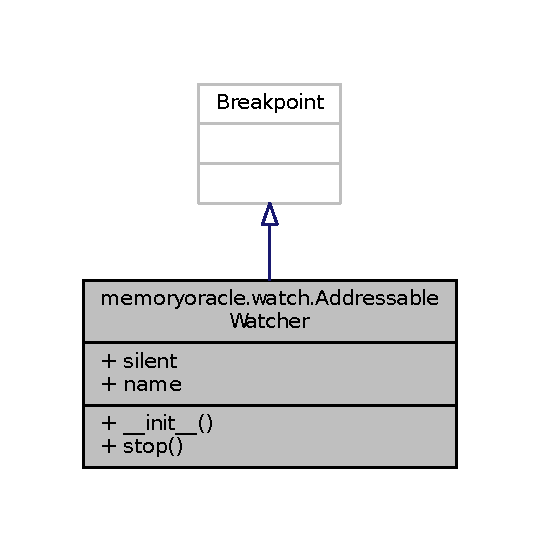
\includegraphics[width=259pt]{classmemoryoracle_1_1watch_1_1AddressableWatcher__inherit__graph}
\end{center}
\end{figure}


Collaboration diagram for memoryoracle.\+watch.\+Addressable\+Watcher\+:\nopagebreak
\begin{figure}[H]
\begin{center}
\leavevmode
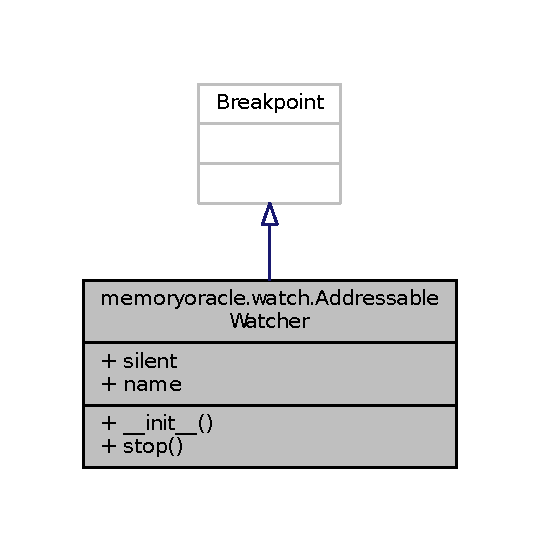
\includegraphics[width=259pt]{classmemoryoracle_1_1watch_1_1AddressableWatcher__coll__graph}
\end{center}
\end{figure}
\subsection*{Public Member Functions}
\begin{DoxyCompactItemize}
\item 
def \hyperlink{classmemoryoracle_1_1watch_1_1AddressableWatcher_a5a534586bb83ff923873c878e4c94c39}{\+\_\+\+\_\+init\+\_\+\+\_\+} (self)
\item 
def \hyperlink{classmemoryoracle_1_1watch_1_1AddressableWatcher_a9db9d7d3b1a32e74ebecb3cdb2537015}{stop} (self)
\end{DoxyCompactItemize}
\subsection*{Public Attributes}
\begin{DoxyCompactItemize}
\item 
\hyperlink{classmemoryoracle_1_1watch_1_1AddressableWatcher_aae157cf9b50d98e099a2c7f98b25634e}{silent}
\item 
\hyperlink{classmemoryoracle_1_1watch_1_1AddressableWatcher_a7b7679f54a21d0a3efc5e785df46186e}{name}
\end{DoxyCompactItemize}


\subsection{Detailed Description}


Definition at line 28 of file watch.\+py.



\subsection{Constructor \& Destructor Documentation}
\hypertarget{classmemoryoracle_1_1watch_1_1AddressableWatcher_a5a534586bb83ff923873c878e4c94c39}{}\index{memoryoracle\+::watch\+::\+Addressable\+Watcher@{memoryoracle\+::watch\+::\+Addressable\+Watcher}!\+\_\+\+\_\+init\+\_\+\+\_\+@{\+\_\+\+\_\+init\+\_\+\+\_\+}}
\index{\+\_\+\+\_\+init\+\_\+\+\_\+@{\+\_\+\+\_\+init\+\_\+\+\_\+}!memoryoracle\+::watch\+::\+Addressable\+Watcher@{memoryoracle\+::watch\+::\+Addressable\+Watcher}}
\subsubsection[{\+\_\+\+\_\+init\+\_\+\+\_\+}]{\setlength{\rightskip}{0pt plus 5cm}def memoryoracle.\+watch.\+Addressable\+Watcher.\+\_\+\+\_\+init\+\_\+\+\_\+ (
\begin{DoxyParamCaption}
\item[{}]{self}
\end{DoxyParamCaption}
)}\label{classmemoryoracle_1_1watch_1_1AddressableWatcher_a5a534586bb83ff923873c878e4c94c39}


Definition at line 30 of file watch.\+py.


\begin{DoxyCode}
30     \textcolor{keyword}{def }\hyperlink{classmemoryoracle_1_1watch_1_1AddressableWatcher_a5a534586bb83ff923873c878e4c94c39}{\_\_init\_\_}(self, ):
31         super(StateWatcher, self).\hyperlink{classmemoryoracle_1_1watch_1_1AddressableWatcher_a5a534586bb83ff923873c878e4c94c39}{\_\_init\_\_}(\textcolor{stringliteral}{"*"} + addr,
32                 gdb.BP\_WATCHPOINT,
33                 gdb.WP\_WRITE,
34                 \textcolor{keyword}{True},
35                 \textcolor{keyword}{False})
36         self.\hyperlink{classmemoryoracle_1_1watch_1_1AddressableWatcher_aae157cf9b50d98e099a2c7f98b25634e}{silent} = \textcolor{keyword}{True}
37         self.\hyperlink{classmemoryoracle_1_1watch_1_1AddressableWatcher_a7b7679f54a21d0a3efc5e785df46186e}{name} = name
38 
\end{DoxyCode}


\subsection{Member Function Documentation}
\hypertarget{classmemoryoracle_1_1watch_1_1AddressableWatcher_a9db9d7d3b1a32e74ebecb3cdb2537015}{}\index{memoryoracle\+::watch\+::\+Addressable\+Watcher@{memoryoracle\+::watch\+::\+Addressable\+Watcher}!stop@{stop}}
\index{stop@{stop}!memoryoracle\+::watch\+::\+Addressable\+Watcher@{memoryoracle\+::watch\+::\+Addressable\+Watcher}}
\subsubsection[{stop}]{\setlength{\rightskip}{0pt plus 5cm}def memoryoracle.\+watch.\+Addressable\+Watcher.\+stop (
\begin{DoxyParamCaption}
\item[{}]{self}
\end{DoxyParamCaption}
)}\label{classmemoryoracle_1_1watch_1_1AddressableWatcher_a9db9d7d3b1a32e74ebecb3cdb2537015}


Definition at line 39 of file watch.\+py.



References memoryoracle.\+execution.\+Instance.\+name, memoryoracle.\+watch.\+Addressable\+Watcher.\+name, memoryoracle.\+execution.\+Executable.\+name, memoryoracle.\+models.\+Tracked.\+name, and memoryoracle.\+instance.\+Memory.\+name.


\begin{DoxyCode}
39     \textcolor{keyword}{def }\hyperlink{classmemoryoracle_1_1watch_1_1AddressableWatcher_a9db9d7d3b1a32e74ebecb3cdb2537015}{stop}(self):
40         frameName = str(gdb.selected\_frame())
41         addr = self.expression[1:]
42         state = State.\_instances.get(frameName, \textcolor{keywordtype}{None})
43 
44         \textcolor{keywordflow}{if} \textcolor{keywordflow}{not} state:
45             state = State()
46             c = state.serialize\_locals()
47             \textcolor{keywordflow}{if} \textcolor{keywordflow}{not} c:
48                 \textcolor{keywordflow}{return} \textcolor{keyword}{False}
49 
50         \textcolor{keywordflow}{try}:
51             val = state.name\_to\_val(self.\hyperlink{classmemoryoracle_1_1watch_1_1AddressableWatcher_a7b7679f54a21d0a3efc5e785df46186e}{name})
52             names = state.get\_serial(val = val).keys()
53             \textcolor{keywordflow}{for} name \textcolor{keywordflow}{in} names:
54                 state.update(val, name)
55 
56         \textcolor{keywordflow}{except} Exception \textcolor{keyword}{as} e:
57             traceback.print\_exc()
58             state.serialize(self.\hyperlink{classmemoryoracle_1_1watch_1_1AddressableWatcher_a7b7679f54a21d0a3efc5e785df46186e}{name}, address = addr)
59             print(\textcolor{stringliteral}{"ERROR: could not find address "} + addr)
60         \textcolor{keywordflow}{return} \textcolor{keyword}{False}
61 
\end{DoxyCode}


\subsection{Member Data Documentation}
\hypertarget{classmemoryoracle_1_1watch_1_1AddressableWatcher_a7b7679f54a21d0a3efc5e785df46186e}{}\index{memoryoracle\+::watch\+::\+Addressable\+Watcher@{memoryoracle\+::watch\+::\+Addressable\+Watcher}!name@{name}}
\index{name@{name}!memoryoracle\+::watch\+::\+Addressable\+Watcher@{memoryoracle\+::watch\+::\+Addressable\+Watcher}}
\subsubsection[{name}]{\setlength{\rightskip}{0pt plus 5cm}memoryoracle.\+watch.\+Addressable\+Watcher.\+name}\label{classmemoryoracle_1_1watch_1_1AddressableWatcher_a7b7679f54a21d0a3efc5e785df46186e}


Definition at line 37 of file watch.\+py.



Referenced by memoryoracle.\+descriptions.\+Memory\+Description.\+dict(), and memoryoracle.\+watch.\+Addressable\+Watcher.\+stop().

\hypertarget{classmemoryoracle_1_1watch_1_1AddressableWatcher_aae157cf9b50d98e099a2c7f98b25634e}{}\index{memoryoracle\+::watch\+::\+Addressable\+Watcher@{memoryoracle\+::watch\+::\+Addressable\+Watcher}!silent@{silent}}
\index{silent@{silent}!memoryoracle\+::watch\+::\+Addressable\+Watcher@{memoryoracle\+::watch\+::\+Addressable\+Watcher}}
\subsubsection[{silent}]{\setlength{\rightskip}{0pt plus 5cm}memoryoracle.\+watch.\+Addressable\+Watcher.\+silent}\label{classmemoryoracle_1_1watch_1_1AddressableWatcher_aae157cf9b50d98e099a2c7f98b25634e}


Definition at line 36 of file watch.\+py.



The documentation for this class was generated from the following file\+:\begin{DoxyCompactItemize}
\item 
memoryoracle/\hyperlink{watch_8py}{watch.\+py}\end{DoxyCompactItemize}

\hypertarget{classmemoryoracle_1_1symbol_1_1Alias}{}\section{memoryoracle.\+symbol.\+Alias Class Reference}
\label{classmemoryoracle_1_1symbol_1_1Alias}\index{memoryoracle.\+symbol.\+Alias@{memoryoracle.\+symbol.\+Alias}}


Inheritance diagram for memoryoracle.\+symbol.\+Alias\+:
\nopagebreak
\begin{figure}[H]
\begin{center}
\leavevmode
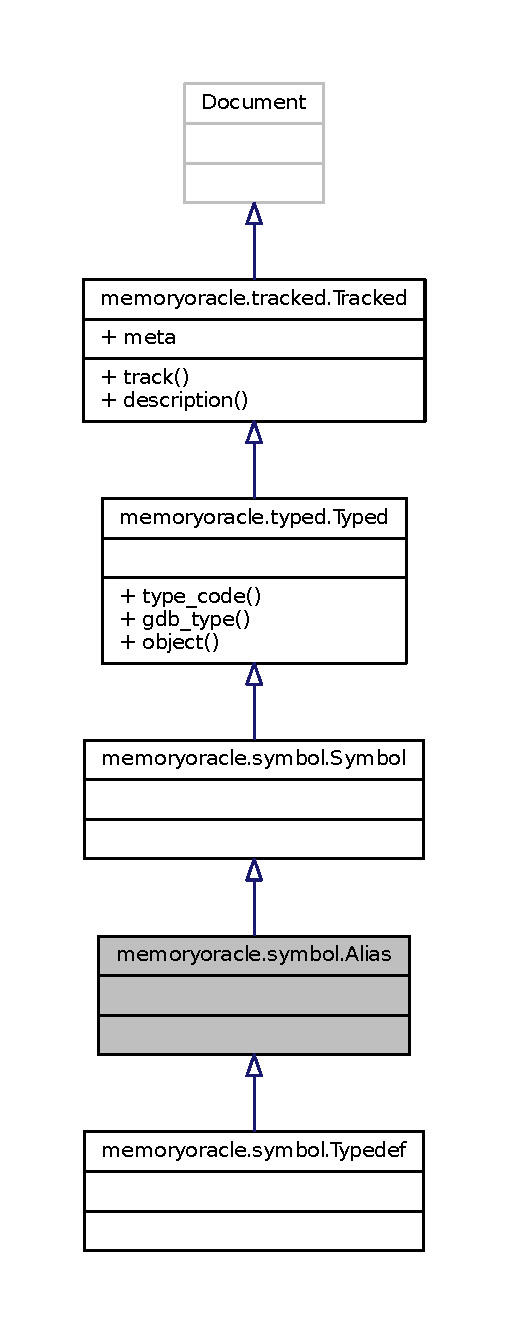
\includegraphics[height=550pt]{classmemoryoracle_1_1symbol_1_1Alias__inherit__graph}
\end{center}
\end{figure}


Collaboration diagram for memoryoracle.\+symbol.\+Alias\+:
\nopagebreak
\begin{figure}[H]
\begin{center}
\leavevmode
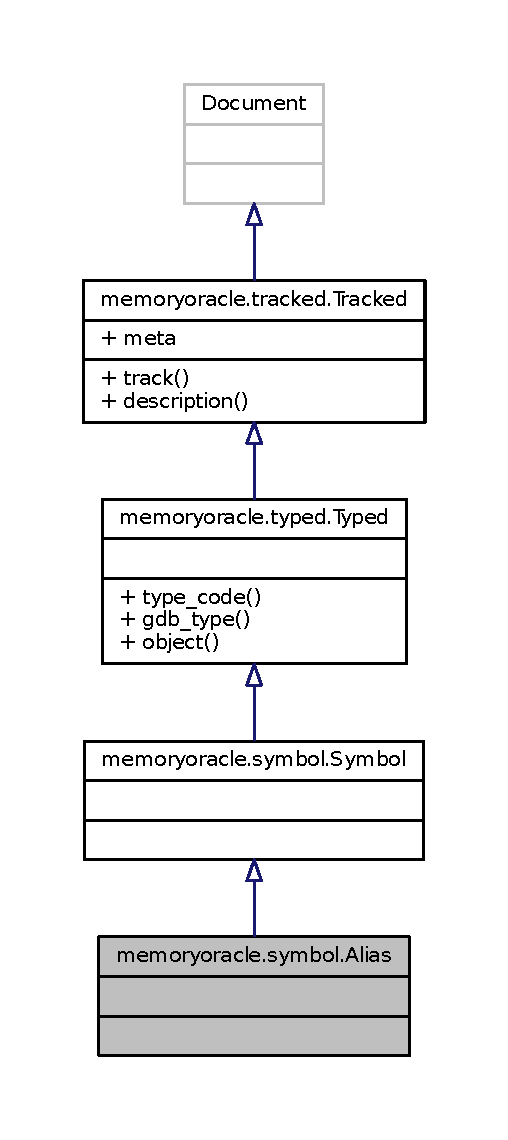
\includegraphics[width=244pt]{classmemoryoracle_1_1symbol_1_1Alias__coll__graph}
\end{center}
\end{figure}
\subsection*{Additional Inherited Members}


\subsection{Detailed Description}


Definition at line 28 of file symbol.\+py.



The documentation for this class was generated from the following file\+:\begin{DoxyCompactItemize}
\item 
memoryoracle/\hyperlink{symbol_8py}{symbol.\+py}\end{DoxyCompactItemize}

\hypertarget{classmemoryoracle_1_1instance_1_1Array}{}\section{memoryoracle.\+instance.\+Array Class Reference}
\label{classmemoryoracle_1_1instance_1_1Array}\index{memoryoracle.\+instance.\+Array@{memoryoracle.\+instance.\+Array}}


Inheritance diagram for memoryoracle.\+instance.\+Array\+:
\nopagebreak
\begin{figure}[H]
\begin{center}
\leavevmode
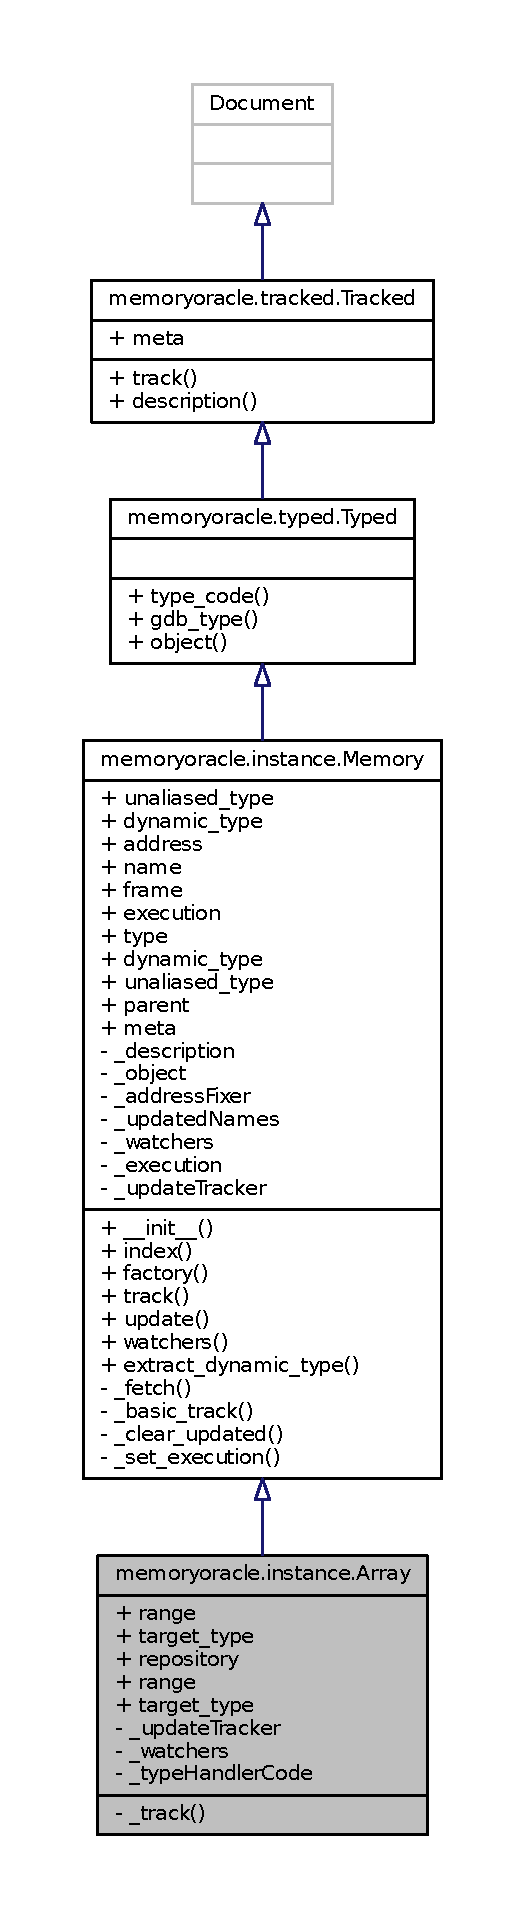
\includegraphics[height=550pt]{classmemoryoracle_1_1instance_1_1Array__inherit__graph}
\end{center}
\end{figure}


Collaboration diagram for memoryoracle.\+instance.\+Array\+:
\nopagebreak
\begin{figure}[H]
\begin{center}
\leavevmode
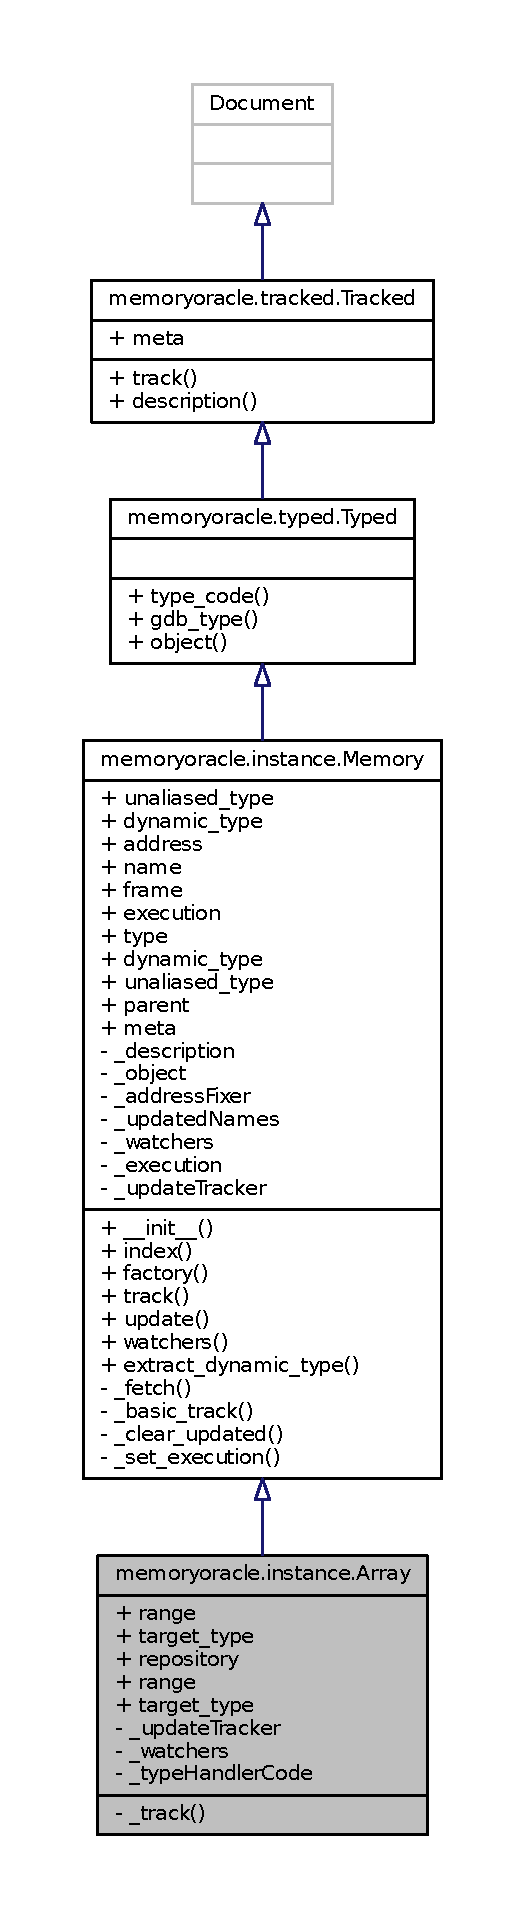
\includegraphics[height=550pt]{classmemoryoracle_1_1instance_1_1Array__coll__graph}
\end{center}
\end{figure}
\subsection*{Public Attributes}
\begin{DoxyCompactItemize}
\item 
\hyperlink{classmemoryoracle_1_1instance_1_1Array_a8bf8e1844305ec3dc5d73ec1ed8c5ba3}{range}
\item 
\hyperlink{classmemoryoracle_1_1instance_1_1Array_aa69695506b2de9ec3336d03efb4fea09}{target\+\_\+type}
\end{DoxyCompactItemize}
\subsection*{Static Public Attributes}
\begin{DoxyCompactItemize}
\item 
tuple \hyperlink{classmemoryoracle_1_1instance_1_1Array_ae8a854bbb76db4aa9661677964d99846}{repository} = dict()
\item 
tuple \hyperlink{classmemoryoracle_1_1instance_1_1Array_acb456ee173f41d41e16e1bebfba48aa6}{range} = mongoengine.\+List\+Field()
\item 
tuple \hyperlink{classmemoryoracle_1_1instance_1_1Array_a23836ff62d41326159a9a47ad3813e38}{target\+\_\+type} = mongoengine.\+String\+Field()
\end{DoxyCompactItemize}
\subsection*{Private Member Functions}
\begin{DoxyCompactItemize}
\item 
def \hyperlink{classmemoryoracle_1_1instance_1_1Array_a1d8c3993d8a52bfbec8240d6f79b3ce1}{\+\_\+track} (self)
\begin{DoxyCompactList}\small\item\em T\+O\+D\+O\+: upgrade this to ref field. \end{DoxyCompactList}\end{DoxyCompactItemize}
\subsection*{Static Private Attributes}
\begin{DoxyCompactItemize}
\item 
tuple \hyperlink{classmemoryoracle_1_1instance_1_1Array_acbb6dbe2e7651d120b69fb39ad808b69}{\+\_\+update\+Tracker} = set()
\item 
tuple \hyperlink{classmemoryoracle_1_1instance_1_1Array_a339afab4d326c225b0a95ee0cabcc19a}{\+\_\+watchers} = dict()
\item 
\hyperlink{classmemoryoracle_1_1instance_1_1Array_a768da780abb79bd63ffc4e47f920de51}{\+\_\+type\+Handler\+Code} = gdb.\+T\+Y\+P\+E\+\_\+\+C\+O\+D\+E\+\_\+\+A\+R\+R\+A\+Y
\end{DoxyCompactItemize}
\subsection*{Additional Inherited Members}


\subsection{Detailed Description}
\begin{DoxyVerb}*Concrete* class to represent an array in the debugge.
\end{DoxyVerb}
 

Definition at line 263 of file instance.\+py.



\subsection{Member Function Documentation}
\hypertarget{classmemoryoracle_1_1instance_1_1Array_a1d8c3993d8a52bfbec8240d6f79b3ce1}{}\index{memoryoracle\+::instance\+::\+Array@{memoryoracle\+::instance\+::\+Array}!\+\_\+track@{\+\_\+track}}
\index{\+\_\+track@{\+\_\+track}!memoryoracle\+::instance\+::\+Array@{memoryoracle\+::instance\+::\+Array}}
\subsubsection[{\+\_\+track}]{\setlength{\rightskip}{0pt plus 5cm}def memoryoracle.\+instance.\+Array.\+\_\+track (
\begin{DoxyParamCaption}
\item[{}]{self}
\end{DoxyParamCaption}
)\hspace{0.3cm}{\ttfamily [private]}}\label{classmemoryoracle_1_1instance_1_1Array_a1d8c3993d8a52bfbec8240d6f79b3ce1}


T\+O\+D\+O\+: upgrade this to ref field. 



Definition at line 277 of file instance.\+py.



References memoryoracle.\+typed.\+Typed.\+object(), and memoryoracle.\+descriptions.\+Memory\+Description.\+object().



Referenced by memoryoracle.\+instance.\+Memory.\+track(), and memoryoracle.\+models.\+Typed.\+track().


\begin{DoxyCode}
277     \textcolor{keyword}{def }\hyperlink{classmemoryoracle_1_1instance_1_1Array_a1d8c3993d8a52bfbec8240d6f79b3ce1}{\_track}(self):
278         \textcolor{comment}{# convenience vars:}
279         s = self.\hyperlink{classmemoryoracle_1_1typed_1_1Typed_a0d1a3c7644d37da66f9ea5cb269115fe}{object}
280 
281         \textcolor{comment}{# compute range of array in C sizeof(type) units}
282         arrayRange = self.object.type.range()
283         self.\hyperlink{classmemoryoracle_1_1instance_1_1Array_acb456ee173f41d41e16e1bebfba48aa6}{range} = arrayRange
284 
285         \textcolor{comment}{# compute the type of data the array contains}
286         \textcolor{comment}{# e.g. for float[2] the answer is float}
287         \textcolor{comment}{# for float[3][2][7] the answer is float}
288         self.\hyperlink{classmemoryoracle_1_1instance_1_1Array_a23836ff62d41326159a9a47ad3813e38}{target\_type} = \hyperlink{namespacememoryoracle_1_1instance_a4b8eb263a612b709be51201fc0fa7b6c}{target\_type\_name}(self.\hyperlink{classmemoryoracle_1_1instance_1_1Memory_a17b9f6c0f548bf201e4fc636c133470b}{type})
289 
290         \textcolor{comment}{# compute the immediate type of data the array}
291         \textcolor{comment}{# contains.  e.g. for float[2] the answer is float.}
292         \textcolor{comment}{# for float[3][2][7] the answer is float[3][2]}
293         immediateTarget = s.type.target()
294 
295         \textcolor{comment}{# if the immediateTarget is an array type, then}
296         \textcolor{comment}{# it will have the same address as the current}
297         \textcolor{comment}{# array.  Still, we want to treat it as as different}
298         \textcolor{comment}{# creature, so we remove the current address}
299         \textcolor{comment}{# from the updateTracker.}
300 
301         \textcolor{comment}{# TODO: if the first element of the array}
302         \textcolor{comment}{# is a pointer back to the array, this may}
303         \textcolor{comment}{# cause an infinite loop.  *This algorithm}
304         \textcolor{comment}{# needs torture testing.*}
305         \textcolor{keywordflow}{if} immediateTarget.code == gdb.TYPE\_CODE\_ARRAY:
306             self.\_updateTracker.remove(self.\hyperlink{classmemoryoracle_1_1instance_1_1Memory_aba9e6136a3854e0ab59a74acd015be06}{index})
307 
308         \textcolor{comment}{# Compute the total length of the array.}
309 
310         \textcolor{comment}{# CONCERN: This should always be correct, but I}
311         \textcolor{comment}{# can't think of a time when the first value of}
312         \textcolor{comment}{# range would be non zero.  Still, this costs}
313         \textcolor{comment}{# very little, and if we support some "1 indexed"}
314         \textcolor{comment}{# langauge, then the algorithm should still work.}
315         \textcolor{keywordflow}{for} i \textcolor{keywordflow}{in} \hyperlink{classmemoryoracle_1_1instance_1_1Array_acb456ee173f41d41e16e1bebfba48aa6}{range}(arrayRange[0], arrayRange[1] + 1):
316             relativeName = \textcolor{stringliteral}{"["} + str(i) + \textcolor{stringliteral}{"]"},
317             childName = self.\hyperlink{classmemoryoracle_1_1instance_1_1Memory_a00f51174e05bcbaa2d0ec3faccbaffaa}{name} + relativeName
318             childDesc = \hyperlink{classmemoryoracle_1_1descriptions_1_1MemoryDescription}{descriptions.MemoryDescription}(
319                 childName,
320                 relativeName=relativeName,
321                 parent=self,
322                 parent\_class=\textcolor{stringliteral}{"array"})
323 
324             childObj = \hyperlink{namespacememoryoracle_1_1instance_ac651a8635b1ae2ee7e788bf9adb17a0b}{addressable\_factory}(childDesc)
325             childObj.track()
326 
327 
328 \textcolor{comment}{# Register the Array class with the type handler}
329 \hyperlink{classmemoryoracle_1_1registry_1_1TypeRegistration}{registry.TypeRegistration}(Array)
330 
331 
\end{DoxyCode}


Here is the call graph for this function\+:
\nopagebreak
\begin{figure}[H]
\begin{center}
\leavevmode
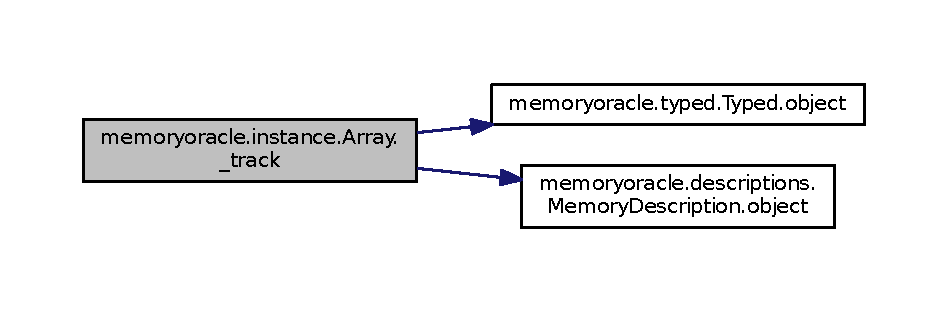
\includegraphics[width=350pt]{classmemoryoracle_1_1instance_1_1Array_a1d8c3993d8a52bfbec8240d6f79b3ce1_cgraph}
\end{center}
\end{figure}




Here is the caller graph for this function\+:
\nopagebreak
\begin{figure}[H]
\begin{center}
\leavevmode
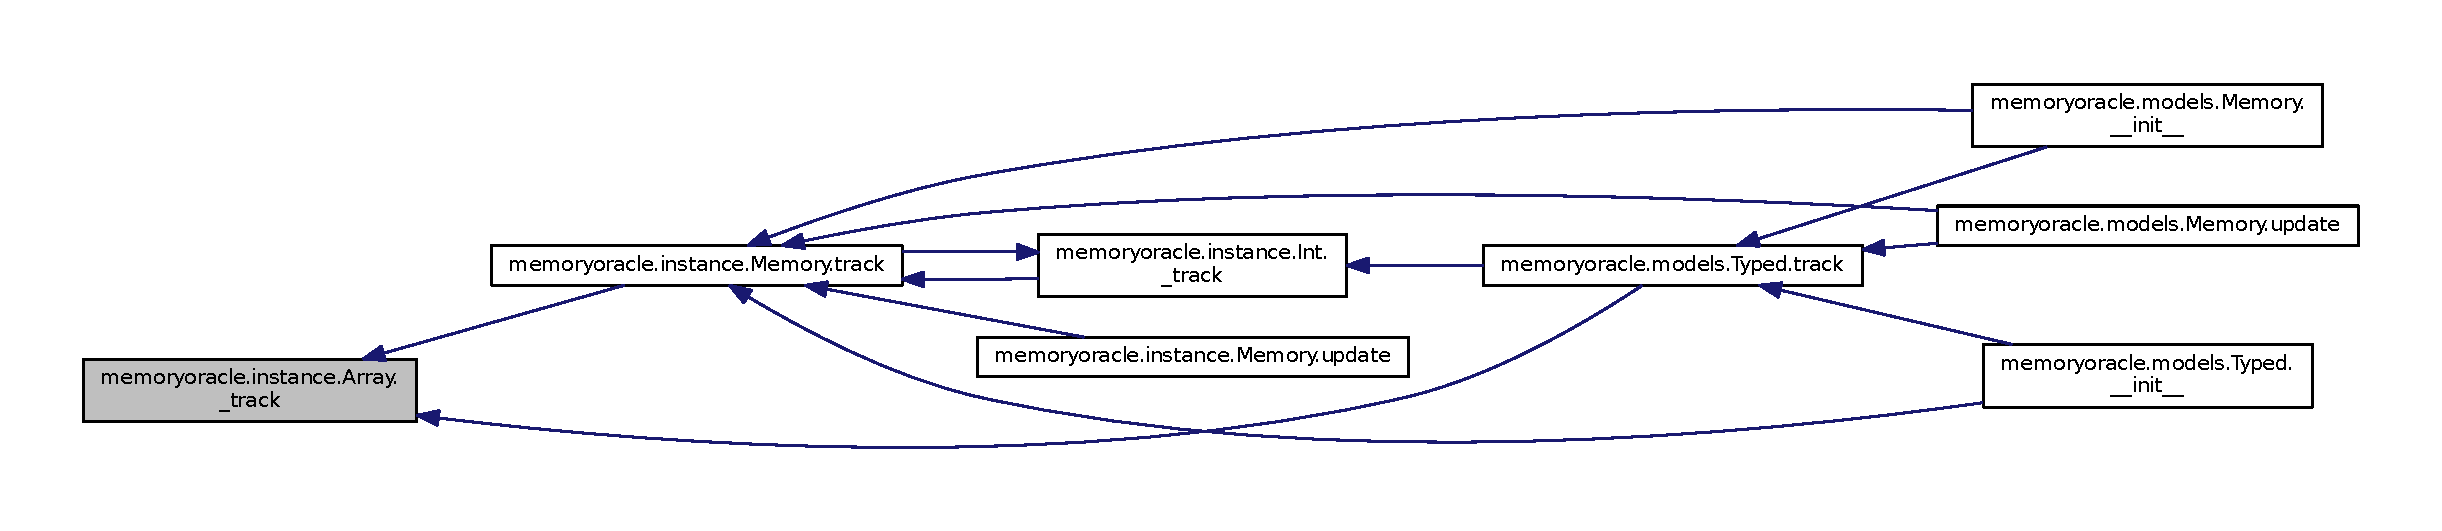
\includegraphics[width=350pt]{classmemoryoracle_1_1instance_1_1Array_a1d8c3993d8a52bfbec8240d6f79b3ce1_icgraph}
\end{center}
\end{figure}




\subsection{Member Data Documentation}
\hypertarget{classmemoryoracle_1_1instance_1_1Array_a768da780abb79bd63ffc4e47f920de51}{}\index{memoryoracle\+::instance\+::\+Array@{memoryoracle\+::instance\+::\+Array}!\+\_\+type\+Handler\+Code@{\+\_\+type\+Handler\+Code}}
\index{\+\_\+type\+Handler\+Code@{\+\_\+type\+Handler\+Code}!memoryoracle\+::instance\+::\+Array@{memoryoracle\+::instance\+::\+Array}}
\subsubsection[{\+\_\+type\+Handler\+Code}]{\setlength{\rightskip}{0pt plus 5cm}memoryoracle.\+instance.\+Array.\+\_\+type\+Handler\+Code = gdb.\+T\+Y\+P\+E\+\_\+\+C\+O\+D\+E\+\_\+\+A\+R\+R\+A\+Y\hspace{0.3cm}{\ttfamily [static]}, {\ttfamily [private]}}\label{classmemoryoracle_1_1instance_1_1Array_a768da780abb79bd63ffc4e47f920de51}


Definition at line 272 of file instance.\+py.



Referenced by memoryoracle.\+models.\+Typed.\+type\+\_\+handler().

\hypertarget{classmemoryoracle_1_1instance_1_1Array_acbb6dbe2e7651d120b69fb39ad808b69}{}\index{memoryoracle\+::instance\+::\+Array@{memoryoracle\+::instance\+::\+Array}!\+\_\+update\+Tracker@{\+\_\+update\+Tracker}}
\index{\+\_\+update\+Tracker@{\+\_\+update\+Tracker}!memoryoracle\+::instance\+::\+Array@{memoryoracle\+::instance\+::\+Array}}
\subsubsection[{\+\_\+update\+Tracker}]{\setlength{\rightskip}{0pt plus 5cm}tuple memoryoracle.\+instance.\+Array.\+\_\+update\+Tracker = set()\hspace{0.3cm}{\ttfamily [static]}, {\ttfamily [private]}}\label{classmemoryoracle_1_1instance_1_1Array_acbb6dbe2e7651d120b69fb39ad808b69}


Definition at line 269 of file instance.\+py.

\hypertarget{classmemoryoracle_1_1instance_1_1Array_a339afab4d326c225b0a95ee0cabcc19a}{}\index{memoryoracle\+::instance\+::\+Array@{memoryoracle\+::instance\+::\+Array}!\+\_\+watchers@{\+\_\+watchers}}
\index{\+\_\+watchers@{\+\_\+watchers}!memoryoracle\+::instance\+::\+Array@{memoryoracle\+::instance\+::\+Array}}
\subsubsection[{\+\_\+watchers}]{\setlength{\rightskip}{0pt plus 5cm}tuple memoryoracle.\+instance.\+Array.\+\_\+watchers = dict()\hspace{0.3cm}{\ttfamily [static]}, {\ttfamily [private]}}\label{classmemoryoracle_1_1instance_1_1Array_a339afab4d326c225b0a95ee0cabcc19a}


Definition at line 270 of file instance.\+py.



Referenced by memoryoracle.\+models.\+Typed.\+\_\+\+\_\+init\+\_\+\+\_\+(), and memoryoracle.\+models.\+Memory.\+watchers().

\hypertarget{classmemoryoracle_1_1instance_1_1Array_acb456ee173f41d41e16e1bebfba48aa6}{}\index{memoryoracle\+::instance\+::\+Array@{memoryoracle\+::instance\+::\+Array}!range@{range}}
\index{range@{range}!memoryoracle\+::instance\+::\+Array@{memoryoracle\+::instance\+::\+Array}}
\subsubsection[{range}]{\setlength{\rightskip}{0pt plus 5cm}tuple memoryoracle.\+instance.\+Array.\+range = mongoengine.\+List\+Field()\hspace{0.3cm}{\ttfamily [static]}}\label{classmemoryoracle_1_1instance_1_1Array_acb456ee173f41d41e16e1bebfba48aa6}


Definition at line 274 of file instance.\+py.

\hypertarget{classmemoryoracle_1_1instance_1_1Array_a8bf8e1844305ec3dc5d73ec1ed8c5ba3}{}\index{memoryoracle\+::instance\+::\+Array@{memoryoracle\+::instance\+::\+Array}!range@{range}}
\index{range@{range}!memoryoracle\+::instance\+::\+Array@{memoryoracle\+::instance\+::\+Array}}
\subsubsection[{range}]{\setlength{\rightskip}{0pt plus 5cm}memoryoracle.\+instance.\+Array.\+range}\label{classmemoryoracle_1_1instance_1_1Array_a8bf8e1844305ec3dc5d73ec1ed8c5ba3}


Definition at line 283 of file instance.\+py.

\hypertarget{classmemoryoracle_1_1instance_1_1Array_ae8a854bbb76db4aa9661677964d99846}{}\index{memoryoracle\+::instance\+::\+Array@{memoryoracle\+::instance\+::\+Array}!repository@{repository}}
\index{repository@{repository}!memoryoracle\+::instance\+::\+Array@{memoryoracle\+::instance\+::\+Array}}
\subsubsection[{repository}]{\setlength{\rightskip}{0pt plus 5cm}tuple memoryoracle.\+instance.\+Array.\+repository = dict()\hspace{0.3cm}{\ttfamily [static]}}\label{classmemoryoracle_1_1instance_1_1Array_ae8a854bbb76db4aa9661677964d99846}


Definition at line 268 of file instance.\+py.

\hypertarget{classmemoryoracle_1_1instance_1_1Array_a23836ff62d41326159a9a47ad3813e38}{}\index{memoryoracle\+::instance\+::\+Array@{memoryoracle\+::instance\+::\+Array}!target\+\_\+type@{target\+\_\+type}}
\index{target\+\_\+type@{target\+\_\+type}!memoryoracle\+::instance\+::\+Array@{memoryoracle\+::instance\+::\+Array}}
\subsubsection[{target\+\_\+type}]{\setlength{\rightskip}{0pt plus 5cm}tuple memoryoracle.\+instance.\+Array.\+target\+\_\+type = mongoengine.\+String\+Field()\hspace{0.3cm}{\ttfamily [static]}}\label{classmemoryoracle_1_1instance_1_1Array_a23836ff62d41326159a9a47ad3813e38}


Definition at line 275 of file instance.\+py.

\hypertarget{classmemoryoracle_1_1instance_1_1Array_aa69695506b2de9ec3336d03efb4fea09}{}\index{memoryoracle\+::instance\+::\+Array@{memoryoracle\+::instance\+::\+Array}!target\+\_\+type@{target\+\_\+type}}
\index{target\+\_\+type@{target\+\_\+type}!memoryoracle\+::instance\+::\+Array@{memoryoracle\+::instance\+::\+Array}}
\subsubsection[{target\+\_\+type}]{\setlength{\rightskip}{0pt plus 5cm}memoryoracle.\+instance.\+Array.\+target\+\_\+type}\label{classmemoryoracle_1_1instance_1_1Array_aa69695506b2de9ec3336d03efb4fea09}


Definition at line 288 of file instance.\+py.



The documentation for this class was generated from the following file\+:\begin{DoxyCompactItemize}
\item 
memoryoracle/\hyperlink{instance_8py}{instance.\+py}\end{DoxyCompactItemize}

\hypertarget{classmemoryoracle_1_1descriptions_1_1BlackBoxDecorator}{}\section{memoryoracle.\+descriptions.\+Black\+Box\+Decorator Class Reference}
\label{classmemoryoracle_1_1descriptions_1_1BlackBoxDecorator}\index{memoryoracle.\+descriptions.\+Black\+Box\+Decorator@{memoryoracle.\+descriptions.\+Black\+Box\+Decorator}}


Inheritance diagram for memoryoracle.\+descriptions.\+Black\+Box\+Decorator\+:\nopagebreak
\begin{figure}[H]
\begin{center}
\leavevmode
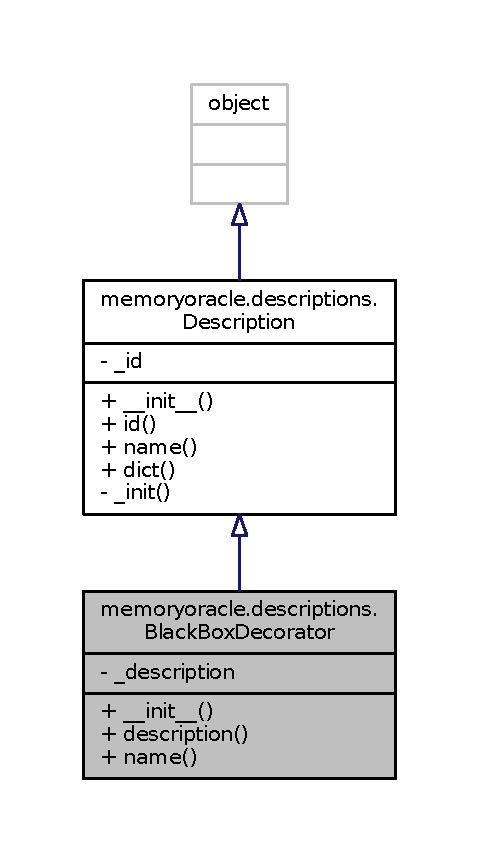
\includegraphics[width=230pt]{classmemoryoracle_1_1descriptions_1_1BlackBoxDecorator__inherit__graph}
\end{center}
\end{figure}


Collaboration diagram for memoryoracle.\+descriptions.\+Black\+Box\+Decorator\+:\nopagebreak
\begin{figure}[H]
\begin{center}
\leavevmode
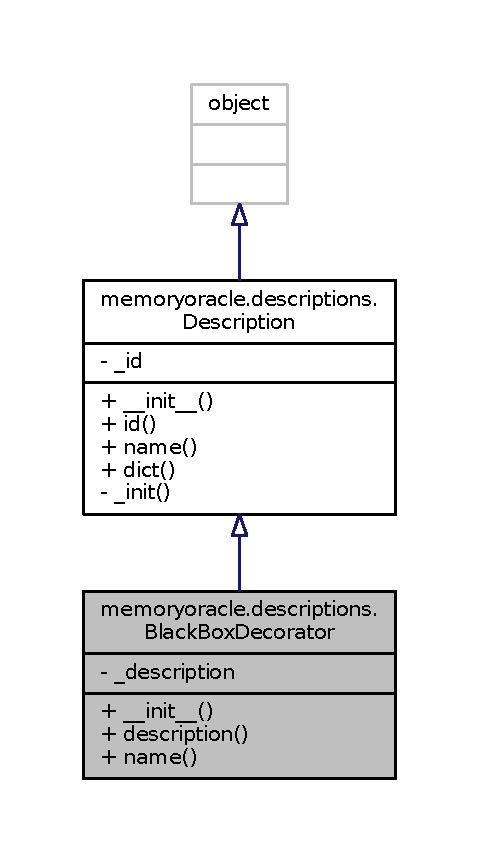
\includegraphics[width=230pt]{classmemoryoracle_1_1descriptions_1_1BlackBoxDecorator__coll__graph}
\end{center}
\end{figure}
\subsection*{Public Member Functions}
\begin{DoxyCompactItemize}
\item 
def \hyperlink{classmemoryoracle_1_1descriptions_1_1BlackBoxDecorator_a157ba0e67a4972c5b9008c36c6127004}{\+\_\+\+\_\+init\+\_\+\+\_\+} (self, \hyperlink{classmemoryoracle_1_1descriptions_1_1BlackBoxDecorator_a558c1ce5d38dc4785d4ef36c0a053967}{description})
\item 
def \hyperlink{classmemoryoracle_1_1descriptions_1_1BlackBoxDecorator_a558c1ce5d38dc4785d4ef36c0a053967}{description} (self)
\item 
def \hyperlink{classmemoryoracle_1_1descriptions_1_1BlackBoxDecorator_a30f3fcba004264fb8b1c4e625a348124}{name} (self)
\end{DoxyCompactItemize}
\subsection*{Private Attributes}
\begin{DoxyCompactItemize}
\item 
\hyperlink{classmemoryoracle_1_1descriptions_1_1BlackBoxDecorator_a4f53f6267b5adff77bdb3ceb92228ee7}{\+\_\+description}
\end{DoxyCompactItemize}


\subsection{Detailed Description}
\begin{DoxyVerb}*Decorator* BlackBoxDecorator class.

A decorator to mark a description as refering to a
piece of information which should not be intrusively
explored by MemoryOracle.
\end{DoxyVerb}
 

Definition at line 41 of file descriptions.\+py.



\subsection{Constructor \& Destructor Documentation}
\hypertarget{classmemoryoracle_1_1descriptions_1_1BlackBoxDecorator_a157ba0e67a4972c5b9008c36c6127004}{}\index{memoryoracle\+::descriptions\+::\+Black\+Box\+Decorator@{memoryoracle\+::descriptions\+::\+Black\+Box\+Decorator}!\+\_\+\+\_\+init\+\_\+\+\_\+@{\+\_\+\+\_\+init\+\_\+\+\_\+}}
\index{\+\_\+\+\_\+init\+\_\+\+\_\+@{\+\_\+\+\_\+init\+\_\+\+\_\+}!memoryoracle\+::descriptions\+::\+Black\+Box\+Decorator@{memoryoracle\+::descriptions\+::\+Black\+Box\+Decorator}}
\subsubsection[{\+\_\+\+\_\+init\+\_\+\+\_\+}]{\setlength{\rightskip}{0pt plus 5cm}def memoryoracle.\+descriptions.\+Black\+Box\+Decorator.\+\_\+\+\_\+init\+\_\+\+\_\+ (
\begin{DoxyParamCaption}
\item[{}]{self, }
\item[{}]{description}
\end{DoxyParamCaption}
)}\label{classmemoryoracle_1_1descriptions_1_1BlackBoxDecorator_a157ba0e67a4972c5b9008c36c6127004}


Definition at line 50 of file descriptions.\+py.


\begin{DoxyCode}
50     \textcolor{keyword}{def }\hyperlink{classmemoryoracle_1_1descriptions_1_1BlackBoxDecorator_a157ba0e67a4972c5b9008c36c6127004}{\_\_init\_\_}(self, description):
51         self.\hyperlink{classmemoryoracle_1_1descriptions_1_1BlackBoxDecorator_a4f53f6267b5adff77bdb3ceb92228ee7}{\_description} = description
52 
\end{DoxyCode}


\subsection{Member Function Documentation}
\hypertarget{classmemoryoracle_1_1descriptions_1_1BlackBoxDecorator_a558c1ce5d38dc4785d4ef36c0a053967}{}\index{memoryoracle\+::descriptions\+::\+Black\+Box\+Decorator@{memoryoracle\+::descriptions\+::\+Black\+Box\+Decorator}!description@{description}}
\index{description@{description}!memoryoracle\+::descriptions\+::\+Black\+Box\+Decorator@{memoryoracle\+::descriptions\+::\+Black\+Box\+Decorator}}
\subsubsection[{description}]{\setlength{\rightskip}{0pt plus 5cm}def memoryoracle.\+descriptions.\+Black\+Box\+Decorator.\+description (
\begin{DoxyParamCaption}
\item[{}]{self}
\end{DoxyParamCaption}
)}\label{classmemoryoracle_1_1descriptions_1_1BlackBoxDecorator_a558c1ce5d38dc4785d4ef36c0a053967}


Definition at line 54 of file descriptions.\+py.



Referenced by memoryoracle.\+instance.\+Int.\+\_\+track().


\begin{DoxyCode}
54     \textcolor{keyword}{def }\hyperlink{classmemoryoracle_1_1descriptions_1_1BlackBoxDecorator_a558c1ce5d38dc4785d4ef36c0a053967}{description}(self):
55         \textcolor{keywordflow}{return} \textcolor{stringliteral}{"---black box---"}
56 
\end{DoxyCode}


Here is the caller graph for this function\+:
\nopagebreak
\begin{figure}[H]
\begin{center}
\leavevmode
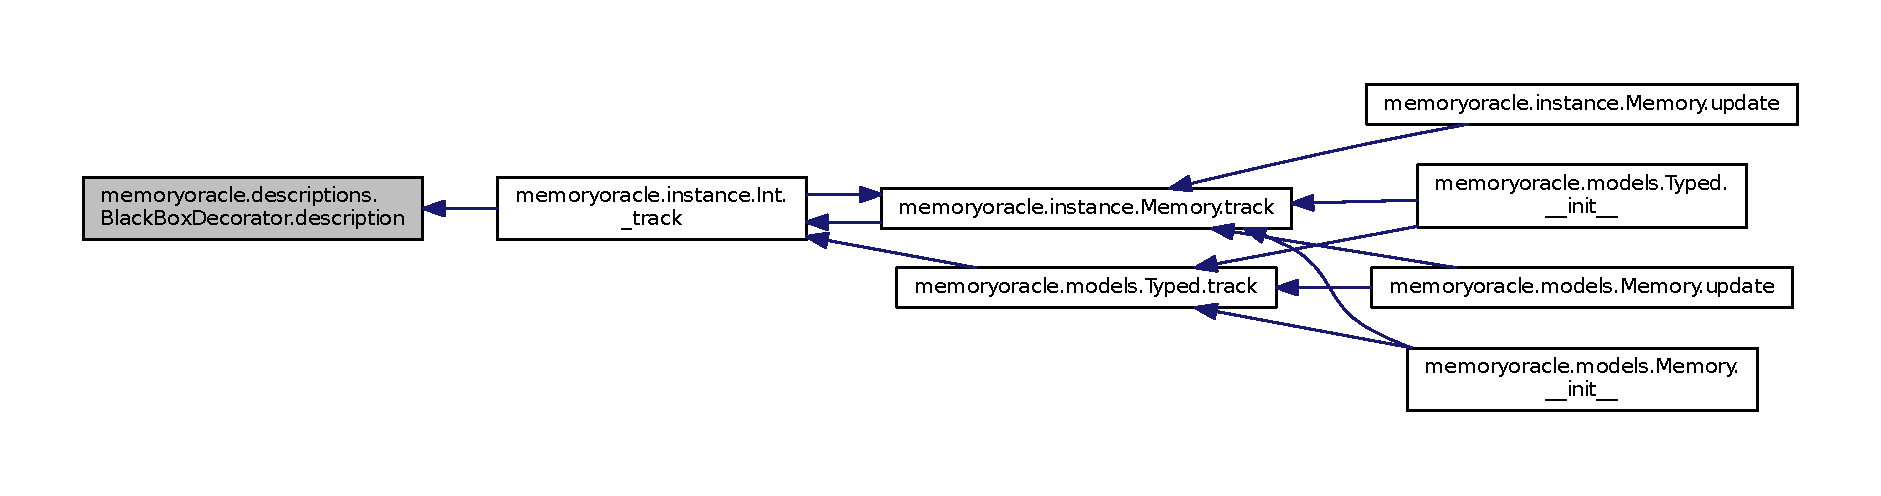
\includegraphics[width=350pt]{classmemoryoracle_1_1descriptions_1_1BlackBoxDecorator_a558c1ce5d38dc4785d4ef36c0a053967_icgraph}
\end{center}
\end{figure}


\hypertarget{classmemoryoracle_1_1descriptions_1_1BlackBoxDecorator_a30f3fcba004264fb8b1c4e625a348124}{}\index{memoryoracle\+::descriptions\+::\+Black\+Box\+Decorator@{memoryoracle\+::descriptions\+::\+Black\+Box\+Decorator}!name@{name}}
\index{name@{name}!memoryoracle\+::descriptions\+::\+Black\+Box\+Decorator@{memoryoracle\+::descriptions\+::\+Black\+Box\+Decorator}}
\subsubsection[{name}]{\setlength{\rightskip}{0pt plus 5cm}def memoryoracle.\+descriptions.\+Black\+Box\+Decorator.\+name (
\begin{DoxyParamCaption}
\item[{}]{self}
\end{DoxyParamCaption}
)}\label{classmemoryoracle_1_1descriptions_1_1BlackBoxDecorator_a30f3fcba004264fb8b1c4e625a348124}


Definition at line 58 of file descriptions.\+py.


\begin{DoxyCode}
58     \textcolor{keyword}{def }\hyperlink{classmemoryoracle_1_1descriptions_1_1BlackBoxDecorator_a30f3fcba004264fb8b1c4e625a348124}{name}(self):
59         \textcolor{keywordflow}{return} self.\_description.name
60 
61 
\end{DoxyCode}


\subsection{Member Data Documentation}
\hypertarget{classmemoryoracle_1_1descriptions_1_1BlackBoxDecorator_a4f53f6267b5adff77bdb3ceb92228ee7}{}\index{memoryoracle\+::descriptions\+::\+Black\+Box\+Decorator@{memoryoracle\+::descriptions\+::\+Black\+Box\+Decorator}!\+\_\+description@{\+\_\+description}}
\index{\+\_\+description@{\+\_\+description}!memoryoracle\+::descriptions\+::\+Black\+Box\+Decorator@{memoryoracle\+::descriptions\+::\+Black\+Box\+Decorator}}
\subsubsection[{\+\_\+description}]{\setlength{\rightskip}{0pt plus 5cm}memoryoracle.\+descriptions.\+Black\+Box\+Decorator.\+\_\+description\hspace{0.3cm}{\ttfamily [private]}}\label{classmemoryoracle_1_1descriptions_1_1BlackBoxDecorator_a4f53f6267b5adff77bdb3ceb92228ee7}


Definition at line 51 of file descriptions.\+py.



Referenced by memoryoracle.\+tracked.\+Tracked.\+description(), memoryoracle.\+descriptions.\+External\+Description\+Decorator.\+description(), and memoryoracle.\+descriptions.\+Standard\+Description\+Decorator.\+description().



The documentation for this class was generated from the following file\+:\begin{DoxyCompactItemize}
\item 
memoryoracle/\hyperlink{descriptions_8py}{descriptions.\+py}\end{DoxyCompactItemize}

\hypertarget{classmemoryoracle_1_1instance_1_1Call}{}\section{memoryoracle.\+instance.\+Call Class Reference}
\label{classmemoryoracle_1_1instance_1_1Call}\index{memoryoracle.\+instance.\+Call@{memoryoracle.\+instance.\+Call}}


Inheritance diagram for memoryoracle.\+instance.\+Call\+:
\nopagebreak
\begin{figure}[H]
\begin{center}
\leavevmode
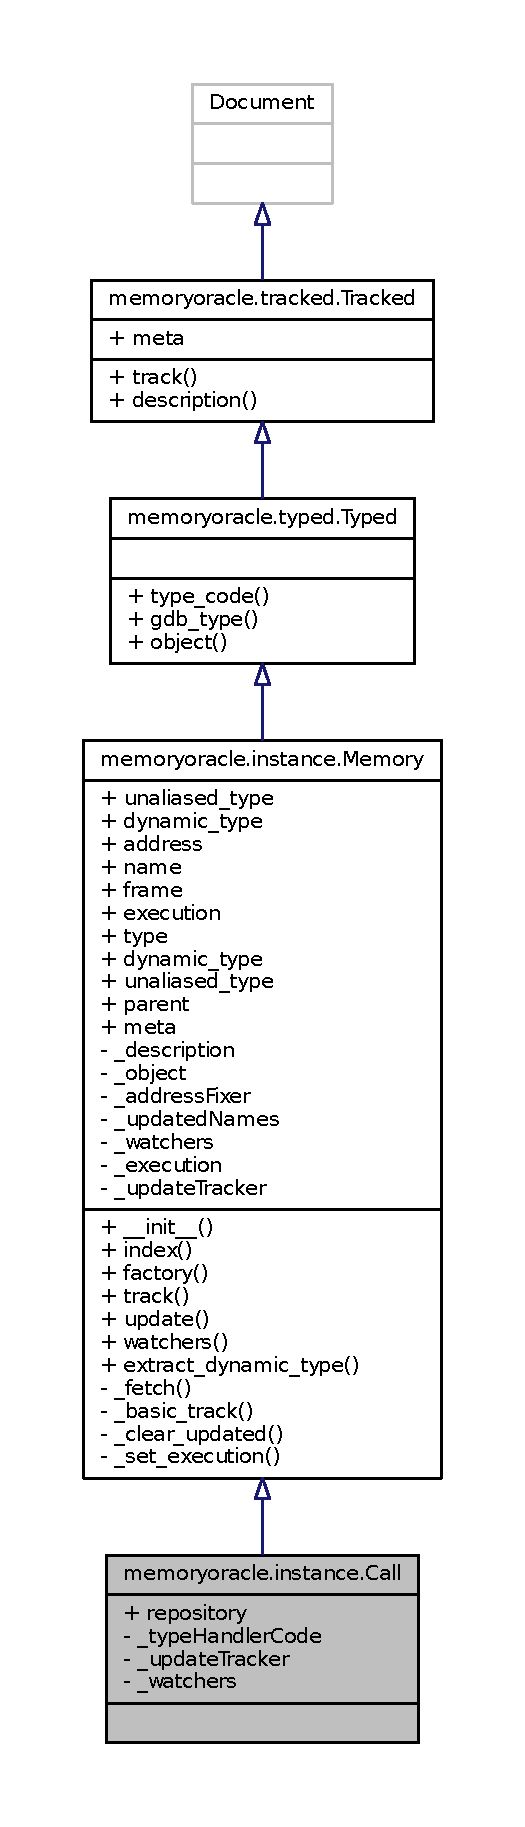
\includegraphics[height=550pt]{classmemoryoracle_1_1instance_1_1Call__inherit__graph}
\end{center}
\end{figure}


Collaboration diagram for memoryoracle.\+instance.\+Call\+:
\nopagebreak
\begin{figure}[H]
\begin{center}
\leavevmode
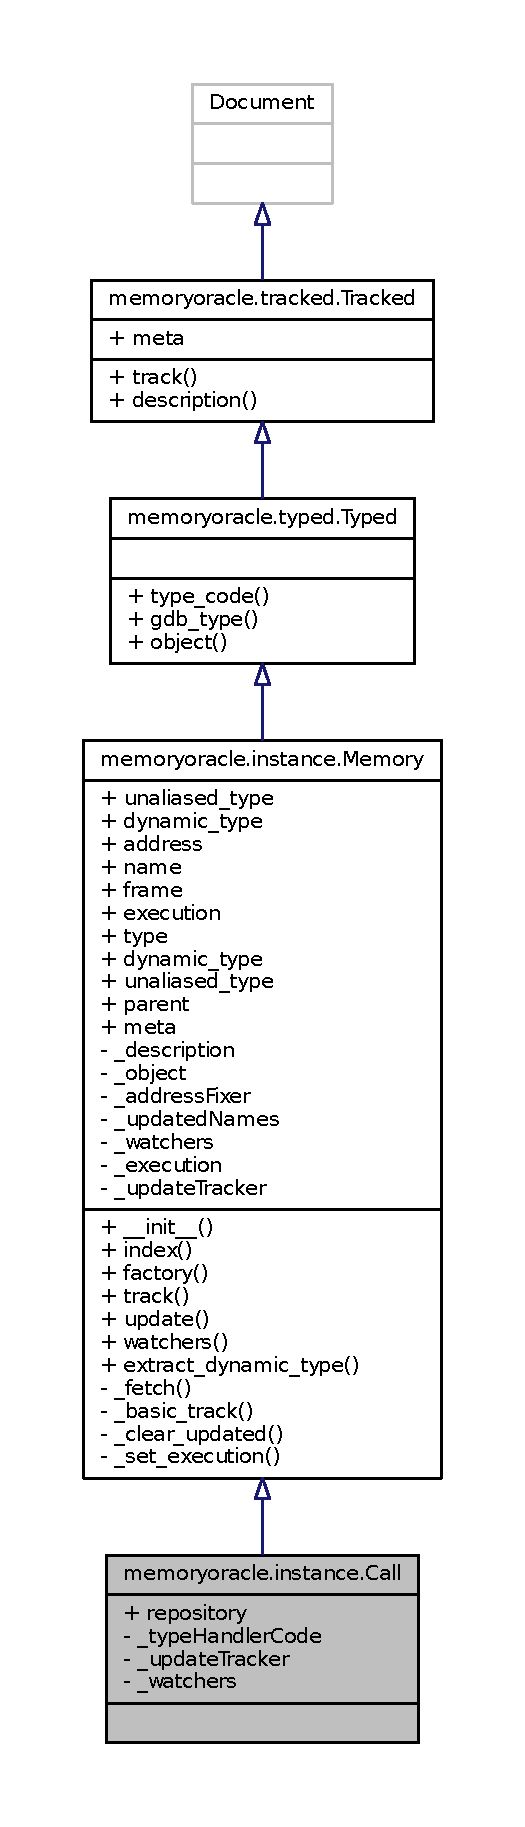
\includegraphics[height=550pt]{classmemoryoracle_1_1instance_1_1Call__coll__graph}
\end{center}
\end{figure}
\subsection*{Static Public Attributes}
\begin{DoxyCompactItemize}
\item 
tuple \hyperlink{classmemoryoracle_1_1instance_1_1Call_a8dc27177c9f423bd7127478c9865208a}{repository} = dict()
\end{DoxyCompactItemize}
\subsection*{Static Private Attributes}
\begin{DoxyCompactItemize}
\item 
\hyperlink{classmemoryoracle_1_1instance_1_1Call_a17f99d3b609b7411bb0a02bac6fe21b7}{\+\_\+type\+Handler\+Code} = gdb.\+T\+Y\+P\+E\+\_\+\+C\+O\+D\+E\+\_\+\+F\+U\+N\+C
\item 
tuple \hyperlink{classmemoryoracle_1_1instance_1_1Call_a21a428f75b5e01781715644c36667ba1}{\+\_\+update\+Tracker} = set()
\item 
tuple \hyperlink{classmemoryoracle_1_1instance_1_1Call_a5584ef8567d815a51e59216116b0c70c}{\+\_\+watchers} = dict()
\end{DoxyCompactItemize}
\subsection*{Additional Inherited Members}


\subsection{Detailed Description}
\begin{DoxyVerb}*Concrete* class representing a particaular call to a function.

This includes class / struct member functions, but does not
include gdb Xmethods or similar.
\end{DoxyVerb}
 

Definition at line 174 of file instance.\+py.



\subsection{Member Data Documentation}
\hypertarget{classmemoryoracle_1_1instance_1_1Call_a17f99d3b609b7411bb0a02bac6fe21b7}{}\index{memoryoracle\+::instance\+::\+Call@{memoryoracle\+::instance\+::\+Call}!\+\_\+type\+Handler\+Code@{\+\_\+type\+Handler\+Code}}
\index{\+\_\+type\+Handler\+Code@{\+\_\+type\+Handler\+Code}!memoryoracle\+::instance\+::\+Call@{memoryoracle\+::instance\+::\+Call}}
\subsubsection[{\+\_\+type\+Handler\+Code}]{\setlength{\rightskip}{0pt plus 5cm}memoryoracle.\+instance.\+Call.\+\_\+type\+Handler\+Code = gdb.\+T\+Y\+P\+E\+\_\+\+C\+O\+D\+E\+\_\+\+F\+U\+N\+C\hspace{0.3cm}{\ttfamily [static]}, {\ttfamily [private]}}\label{classmemoryoracle_1_1instance_1_1Call_a17f99d3b609b7411bb0a02bac6fe21b7}


Definition at line 182 of file instance.\+py.



Referenced by memoryoracle.\+models.\+Typed.\+type\+\_\+handler().

\hypertarget{classmemoryoracle_1_1instance_1_1Call_a21a428f75b5e01781715644c36667ba1}{}\index{memoryoracle\+::instance\+::\+Call@{memoryoracle\+::instance\+::\+Call}!\+\_\+update\+Tracker@{\+\_\+update\+Tracker}}
\index{\+\_\+update\+Tracker@{\+\_\+update\+Tracker}!memoryoracle\+::instance\+::\+Call@{memoryoracle\+::instance\+::\+Call}}
\subsubsection[{\+\_\+update\+Tracker}]{\setlength{\rightskip}{0pt plus 5cm}tuple memoryoracle.\+instance.\+Call.\+\_\+update\+Tracker = set()\hspace{0.3cm}{\ttfamily [static]}, {\ttfamily [private]}}\label{classmemoryoracle_1_1instance_1_1Call_a21a428f75b5e01781715644c36667ba1}


Definition at line 183 of file instance.\+py.

\hypertarget{classmemoryoracle_1_1instance_1_1Call_a5584ef8567d815a51e59216116b0c70c}{}\index{memoryoracle\+::instance\+::\+Call@{memoryoracle\+::instance\+::\+Call}!\+\_\+watchers@{\+\_\+watchers}}
\index{\+\_\+watchers@{\+\_\+watchers}!memoryoracle\+::instance\+::\+Call@{memoryoracle\+::instance\+::\+Call}}
\subsubsection[{\+\_\+watchers}]{\setlength{\rightskip}{0pt plus 5cm}tuple memoryoracle.\+instance.\+Call.\+\_\+watchers = dict()\hspace{0.3cm}{\ttfamily [static]}, {\ttfamily [private]}}\label{classmemoryoracle_1_1instance_1_1Call_a5584ef8567d815a51e59216116b0c70c}


Definition at line 184 of file instance.\+py.



Referenced by memoryoracle.\+models.\+Typed.\+\_\+\+\_\+init\+\_\+\+\_\+(), and memoryoracle.\+models.\+Memory.\+watchers().

\hypertarget{classmemoryoracle_1_1instance_1_1Call_a8dc27177c9f423bd7127478c9865208a}{}\index{memoryoracle\+::instance\+::\+Call@{memoryoracle\+::instance\+::\+Call}!repository@{repository}}
\index{repository@{repository}!memoryoracle\+::instance\+::\+Call@{memoryoracle\+::instance\+::\+Call}}
\subsubsection[{repository}]{\setlength{\rightskip}{0pt plus 5cm}tuple memoryoracle.\+instance.\+Call.\+repository = dict()\hspace{0.3cm}{\ttfamily [static]}}\label{classmemoryoracle_1_1instance_1_1Call_a8dc27177c9f423bd7127478c9865208a}


Definition at line 181 of file instance.\+py.



The documentation for this class was generated from the following file\+:\begin{DoxyCompactItemize}
\item 
memoryoracle/\hyperlink{instance_8py}{instance.\+py}\end{DoxyCompactItemize}

\hypertarget{classmemoryoracle_1_1instance_1_1CharString}{}\section{memoryoracle.\+instance.\+Char\+String Class Reference}
\label{classmemoryoracle_1_1instance_1_1CharString}\index{memoryoracle.\+instance.\+Char\+String@{memoryoracle.\+instance.\+Char\+String}}


Inheritance diagram for memoryoracle.\+instance.\+Char\+String\+:
\nopagebreak
\begin{figure}[H]
\begin{center}
\leavevmode
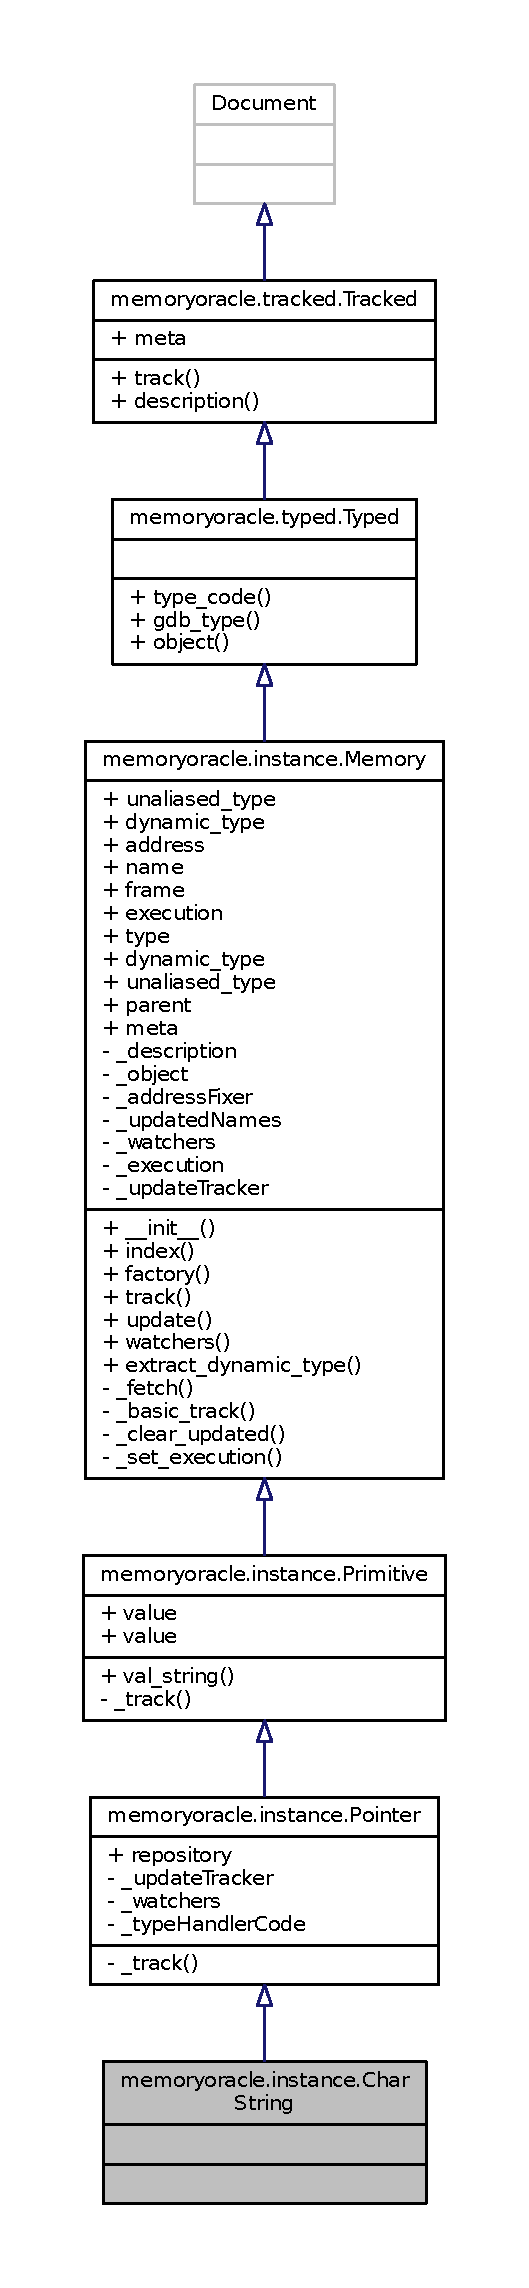
\includegraphics[height=550pt]{classmemoryoracle_1_1instance_1_1CharString__inherit__graph}
\end{center}
\end{figure}


Collaboration diagram for memoryoracle.\+instance.\+Char\+String\+:
\nopagebreak
\begin{figure}[H]
\begin{center}
\leavevmode
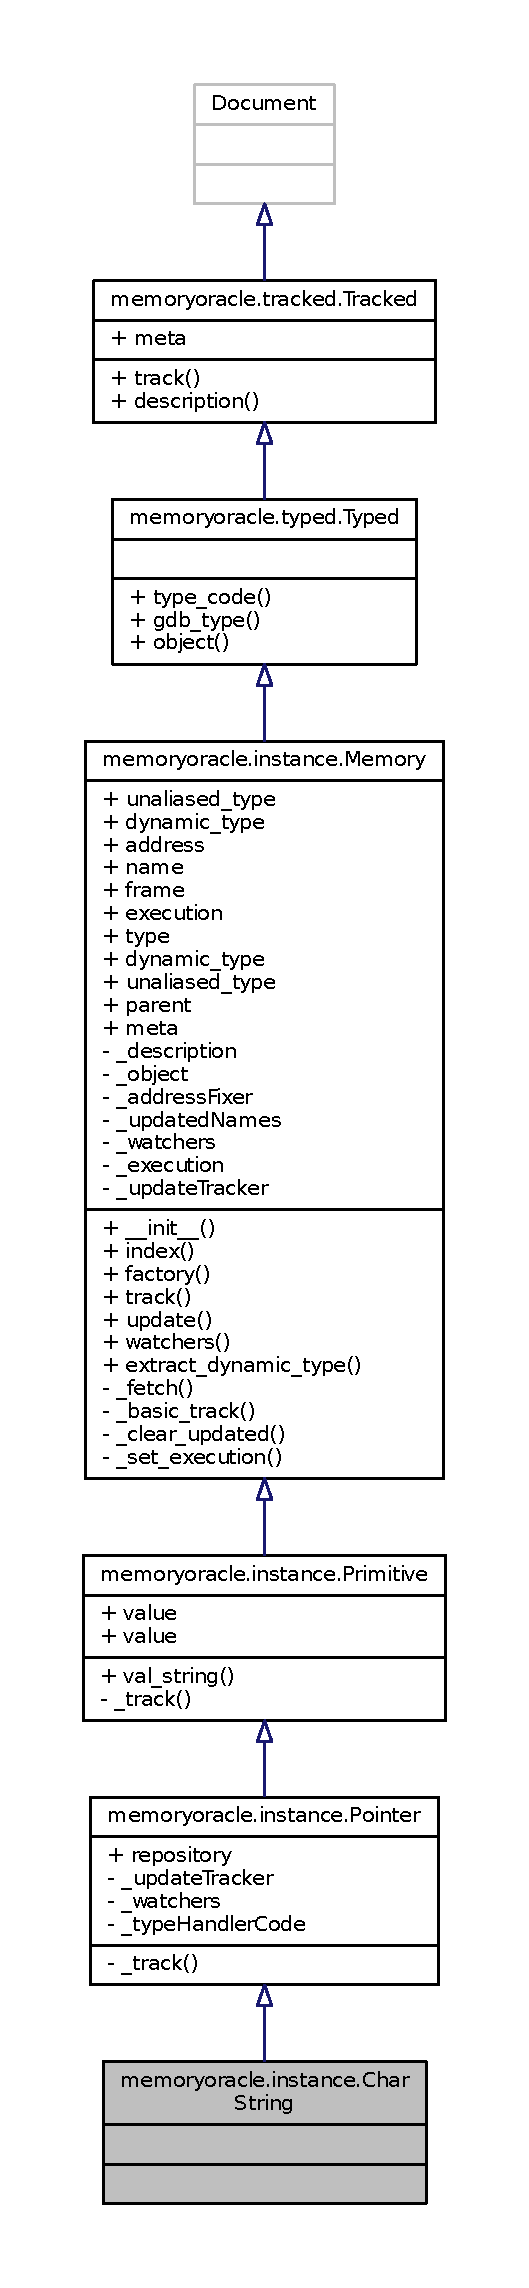
\includegraphics[height=550pt]{classmemoryoracle_1_1instance_1_1CharString__coll__graph}
\end{center}
\end{figure}
\subsection*{Additional Inherited Members}


\subsection{Detailed Description}
\begin{DoxyVerb}*Concrete* class to represent an old style null terminated C string.
\end{DoxyVerb}
 

Definition at line 458 of file instance.\+py.



The documentation for this class was generated from the following file\+:\begin{DoxyCompactItemize}
\item 
memoryoracle/\hyperlink{instance_8py}{instance.\+py}\end{DoxyCompactItemize}

\hypertarget{classmemoryoracle_1_1whip_1_1Coffee}{}\section{memoryoracle.\+whip.\+Coffee Class Reference}
\label{classmemoryoracle_1_1whip_1_1Coffee}\index{memoryoracle.\+whip.\+Coffee@{memoryoracle.\+whip.\+Coffee}}


Inheritance diagram for memoryoracle.\+whip.\+Coffee\+:\nopagebreak
\begin{figure}[H]
\begin{center}
\leavevmode
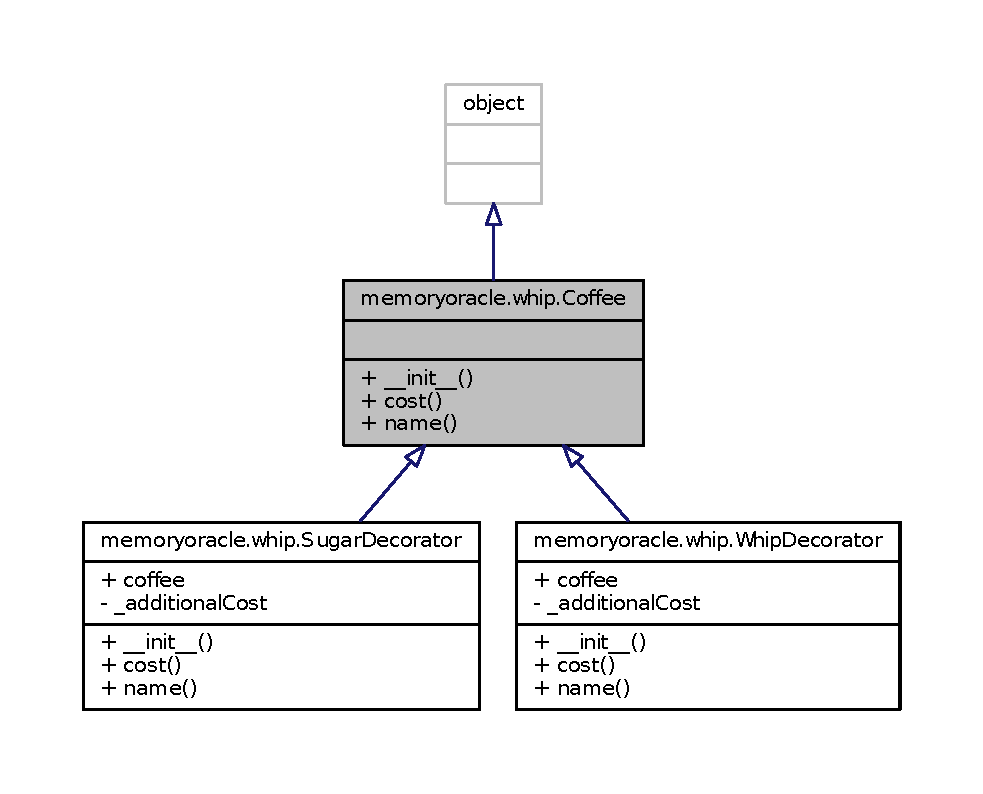
\includegraphics[width=350pt]{classmemoryoracle_1_1whip_1_1Coffee__inherit__graph}
\end{center}
\end{figure}


Collaboration diagram for memoryoracle.\+whip.\+Coffee\+:\nopagebreak
\begin{figure}[H]
\begin{center}
\leavevmode
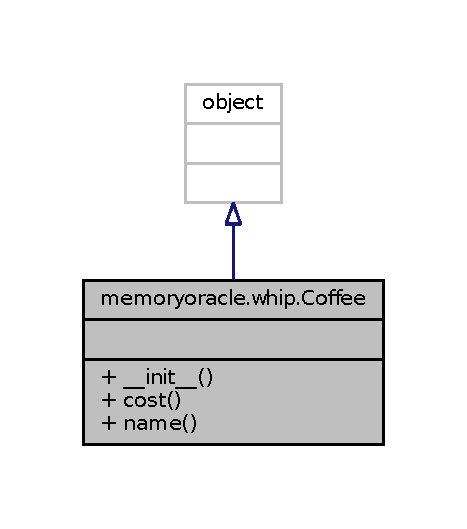
\includegraphics[width=224pt]{classmemoryoracle_1_1whip_1_1Coffee__coll__graph}
\end{center}
\end{figure}
\subsection*{Public Member Functions}
\begin{DoxyCompactItemize}
\item 
def \hyperlink{classmemoryoracle_1_1whip_1_1Coffee_a4b03aa37be53c2de893859b13dbd0d59}{\+\_\+\+\_\+init\+\_\+\+\_\+} (self)
\item 
def \hyperlink{classmemoryoracle_1_1whip_1_1Coffee_a3a48223644953f435dd3d8f6cb3c0b01}{cost} (self)
\item 
def \hyperlink{classmemoryoracle_1_1whip_1_1Coffee_a0d8c38135ee9a8cf701ffb580edf66e3}{name} (self)
\end{DoxyCompactItemize}


\subsection{Detailed Description}


Definition at line 5 of file whip.\+py.



\subsection{Constructor \& Destructor Documentation}
\hypertarget{classmemoryoracle_1_1whip_1_1Coffee_a4b03aa37be53c2de893859b13dbd0d59}{}\index{memoryoracle\+::whip\+::\+Coffee@{memoryoracle\+::whip\+::\+Coffee}!\+\_\+\+\_\+init\+\_\+\+\_\+@{\+\_\+\+\_\+init\+\_\+\+\_\+}}
\index{\+\_\+\+\_\+init\+\_\+\+\_\+@{\+\_\+\+\_\+init\+\_\+\+\_\+}!memoryoracle\+::whip\+::\+Coffee@{memoryoracle\+::whip\+::\+Coffee}}
\subsubsection[{\+\_\+\+\_\+init\+\_\+\+\_\+}]{\setlength{\rightskip}{0pt plus 5cm}def memoryoracle.\+whip.\+Coffee.\+\_\+\+\_\+init\+\_\+\+\_\+ (
\begin{DoxyParamCaption}
\item[{}]{self}
\end{DoxyParamCaption}
)}\label{classmemoryoracle_1_1whip_1_1Coffee_a4b03aa37be53c2de893859b13dbd0d59}


Definition at line 7 of file whip.\+py.


\begin{DoxyCode}
7     \textcolor{keyword}{def }\hyperlink{classmemoryoracle_1_1whip_1_1Coffee_a4b03aa37be53c2de893859b13dbd0d59}{\_\_init\_\_}(self):
8         \textcolor{keywordflow}{pass}
9 
\end{DoxyCode}


\subsection{Member Function Documentation}
\hypertarget{classmemoryoracle_1_1whip_1_1Coffee_a3a48223644953f435dd3d8f6cb3c0b01}{}\index{memoryoracle\+::whip\+::\+Coffee@{memoryoracle\+::whip\+::\+Coffee}!cost@{cost}}
\index{cost@{cost}!memoryoracle\+::whip\+::\+Coffee@{memoryoracle\+::whip\+::\+Coffee}}
\subsubsection[{cost}]{\setlength{\rightskip}{0pt plus 5cm}def memoryoracle.\+whip.\+Coffee.\+cost (
\begin{DoxyParamCaption}
\item[{}]{self}
\end{DoxyParamCaption}
)}\label{classmemoryoracle_1_1whip_1_1Coffee_a3a48223644953f435dd3d8f6cb3c0b01}


Definition at line 10 of file whip.\+py.


\begin{DoxyCode}
10     \textcolor{keyword}{def }\hyperlink{classmemoryoracle_1_1whip_1_1Coffee_a3a48223644953f435dd3d8f6cb3c0b01}{cost}(self):
11         \textcolor{keywordflow}{return} 1.00
12 
\end{DoxyCode}
\hypertarget{classmemoryoracle_1_1whip_1_1Coffee_a0d8c38135ee9a8cf701ffb580edf66e3}{}\index{memoryoracle\+::whip\+::\+Coffee@{memoryoracle\+::whip\+::\+Coffee}!name@{name}}
\index{name@{name}!memoryoracle\+::whip\+::\+Coffee@{memoryoracle\+::whip\+::\+Coffee}}
\subsubsection[{name}]{\setlength{\rightskip}{0pt plus 5cm}def memoryoracle.\+whip.\+Coffee.\+name (
\begin{DoxyParamCaption}
\item[{}]{self}
\end{DoxyParamCaption}
)}\label{classmemoryoracle_1_1whip_1_1Coffee_a0d8c38135ee9a8cf701ffb580edf66e3}


Definition at line 13 of file whip.\+py.


\begin{DoxyCode}
13     \textcolor{keyword}{def }\hyperlink{classmemoryoracle_1_1whip_1_1Coffee_a0d8c38135ee9a8cf701ffb580edf66e3}{name}(self):
14         \textcolor{keywordflow}{return} \textcolor{stringliteral}{"coffee"}
15 
16 
\end{DoxyCode}


The documentation for this class was generated from the following file\+:\begin{DoxyCompactItemize}
\item 
memoryoracle/\hyperlink{whip_8py}{whip.\+py}\end{DoxyCompactItemize}

\hypertarget{classmemoryoracle_1_1execution_1_1Commit}{}\section{memoryoracle.\+execution.\+Commit Class Reference}
\label{classmemoryoracle_1_1execution_1_1Commit}\index{memoryoracle.\+execution.\+Commit@{memoryoracle.\+execution.\+Commit}}


Inheritance diagram for memoryoracle.\+execution.\+Commit\+:\nopagebreak
\begin{figure}[H]
\begin{center}
\leavevmode
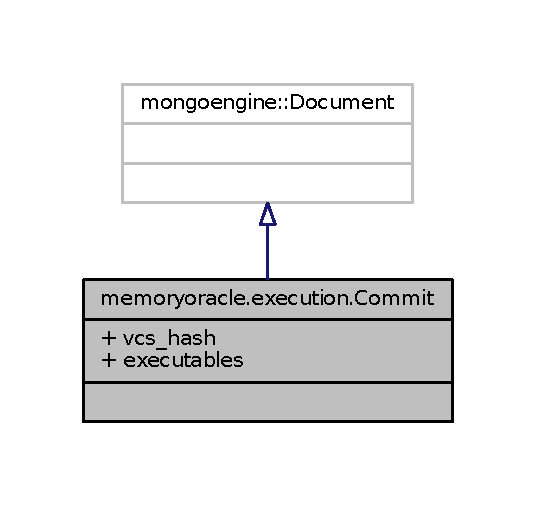
\includegraphics[width=257pt]{classmemoryoracle_1_1execution_1_1Commit__inherit__graph}
\end{center}
\end{figure}


Collaboration diagram for memoryoracle.\+execution.\+Commit\+:\nopagebreak
\begin{figure}[H]
\begin{center}
\leavevmode
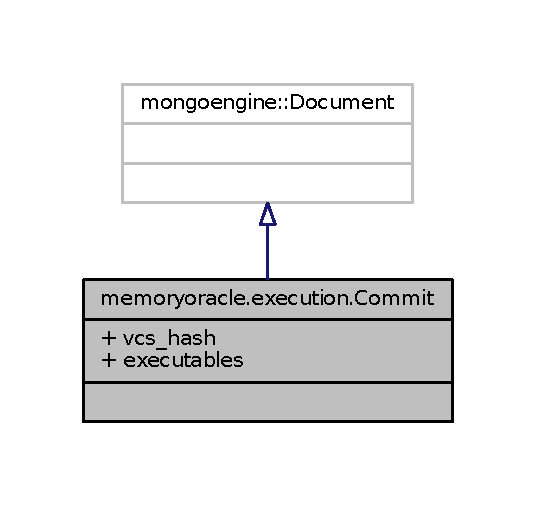
\includegraphics[width=257pt]{classmemoryoracle_1_1execution_1_1Commit__coll__graph}
\end{center}
\end{figure}
\subsection*{Static Public Attributes}
\begin{DoxyCompactItemize}
\item 
tuple \hyperlink{classmemoryoracle_1_1execution_1_1Commit_a3ba32127f9f96216379e06d3fb64fd9b}{vcs\+\_\+hash} = mongoengine.\+String\+Field()
\item 
tuple \hyperlink{classmemoryoracle_1_1execution_1_1Commit_aaefe153fdfeaab0bea861905e8e32f5a}{executables} = mongoengine.\+Embedded\+Document\+List\+Field(\hyperlink{classmemoryoracle_1_1execution_1_1Executable}{Executable})
\end{DoxyCompactItemize}


\subsection{Detailed Description}
\begin{DoxyVerb}*Concrete* class representing a version control system commit.
\end{DoxyVerb}
 

Definition at line 48 of file execution.\+py.



\subsection{Member Data Documentation}
\hypertarget{classmemoryoracle_1_1execution_1_1Commit_aaefe153fdfeaab0bea861905e8e32f5a}{}\index{memoryoracle\+::execution\+::\+Commit@{memoryoracle\+::execution\+::\+Commit}!executables@{executables}}
\index{executables@{executables}!memoryoracle\+::execution\+::\+Commit@{memoryoracle\+::execution\+::\+Commit}}
\subsubsection[{executables}]{\setlength{\rightskip}{0pt plus 5cm}tuple memoryoracle.\+execution.\+Commit.\+executables = mongoengine.\+Embedded\+Document\+List\+Field({\bf Executable})\hspace{0.3cm}{\ttfamily [static]}}\label{classmemoryoracle_1_1execution_1_1Commit_aaefe153fdfeaab0bea861905e8e32f5a}


Definition at line 53 of file execution.\+py.

\hypertarget{classmemoryoracle_1_1execution_1_1Commit_a3ba32127f9f96216379e06d3fb64fd9b}{}\index{memoryoracle\+::execution\+::\+Commit@{memoryoracle\+::execution\+::\+Commit}!vcs\+\_\+hash@{vcs\+\_\+hash}}
\index{vcs\+\_\+hash@{vcs\+\_\+hash}!memoryoracle\+::execution\+::\+Commit@{memoryoracle\+::execution\+::\+Commit}}
\subsubsection[{vcs\+\_\+hash}]{\setlength{\rightskip}{0pt plus 5cm}tuple memoryoracle.\+execution.\+Commit.\+vcs\+\_\+hash = mongoengine.\+String\+Field()\hspace{0.3cm}{\ttfamily [static]}}\label{classmemoryoracle_1_1execution_1_1Commit_a3ba32127f9f96216379e06d3fb64fd9b}


Definition at line 52 of file execution.\+py.



The documentation for this class was generated from the following file\+:\begin{DoxyCompactItemize}
\item 
memoryoracle/\hyperlink{execution_8py}{execution.\+py}\end{DoxyCompactItemize}

\hypertarget{classmemoryoracle_1_1models_1_1Commit}{}\section{memoryoracle.\+models.\+Commit Class Reference}
\label{classmemoryoracle_1_1models_1_1Commit}\index{memoryoracle.\+models.\+Commit@{memoryoracle.\+models.\+Commit}}


Inheritance diagram for memoryoracle.\+models.\+Commit\+:\nopagebreak
\begin{figure}[H]
\begin{center}
\leavevmode
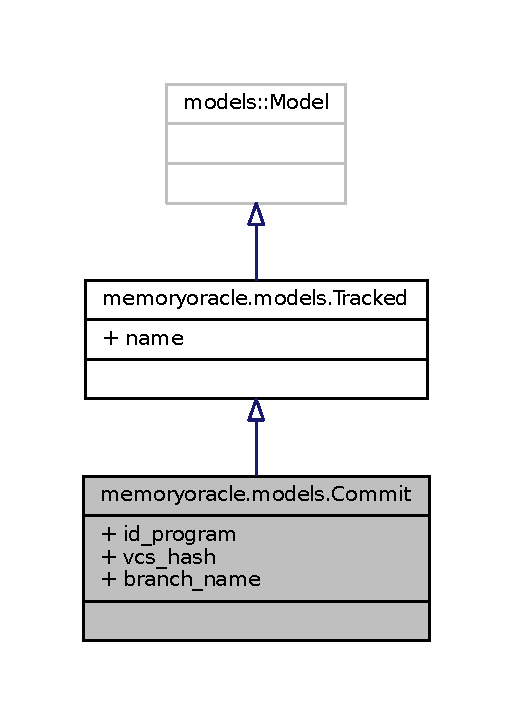
\includegraphics[width=246pt]{classmemoryoracle_1_1models_1_1Commit__inherit__graph}
\end{center}
\end{figure}


Collaboration diagram for memoryoracle.\+models.\+Commit\+:\nopagebreak
\begin{figure}[H]
\begin{center}
\leavevmode
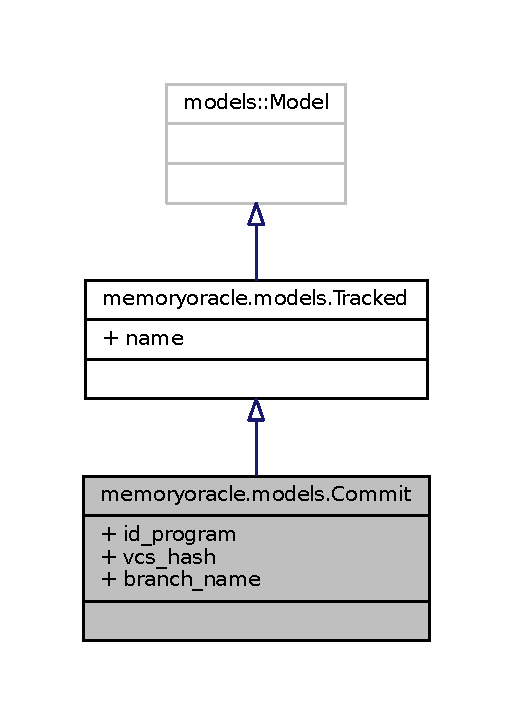
\includegraphics[width=246pt]{classmemoryoracle_1_1models_1_1Commit__coll__graph}
\end{center}
\end{figure}
\subsection*{Classes}
\begin{DoxyCompactItemize}
\item 
class \hyperlink{classmemoryoracle_1_1models_1_1Commit_1_1Meta}{Meta}
\end{DoxyCompactItemize}
\subsection*{Static Public Attributes}
\begin{DoxyCompactItemize}
\item 
tuple \hyperlink{classmemoryoracle_1_1models_1_1Commit_a874612ef3353692531dbdde8f1a17609}{id\+\_\+program} = models.\+Foreign\+Key(\hyperlink{classmemoryoracle_1_1models_1_1Program}{Program})
\item 
tuple \hyperlink{classmemoryoracle_1_1models_1_1Commit_a6c92b2816250c6dfc2ae6f67e94fa472}{vcs\+\_\+hash} = models.\+Char\+Field(unique=True, max\+\_\+length=200)
\item 
tuple \hyperlink{classmemoryoracle_1_1models_1_1Commit_a1ac382bebfef4bd3e24548ad08cda47a}{branch\+\_\+name} = models.\+Char\+Field(max\+\_\+length=200)
\end{DoxyCompactItemize}


\subsection{Detailed Description}


Definition at line 52 of file models.\+py.



\subsection{Member Data Documentation}
\hypertarget{classmemoryoracle_1_1models_1_1Commit_a1ac382bebfef4bd3e24548ad08cda47a}{}\index{memoryoracle\+::models\+::\+Commit@{memoryoracle\+::models\+::\+Commit}!branch\+\_\+name@{branch\+\_\+name}}
\index{branch\+\_\+name@{branch\+\_\+name}!memoryoracle\+::models\+::\+Commit@{memoryoracle\+::models\+::\+Commit}}
\subsubsection[{branch\+\_\+name}]{\setlength{\rightskip}{0pt plus 5cm}tuple memoryoracle.\+models.\+Commit.\+branch\+\_\+name = models.\+Char\+Field(max\+\_\+length=200)\hspace{0.3cm}{\ttfamily [static]}}\label{classmemoryoracle_1_1models_1_1Commit_a1ac382bebfef4bd3e24548ad08cda47a}


Definition at line 56 of file models.\+py.

\hypertarget{classmemoryoracle_1_1models_1_1Commit_a874612ef3353692531dbdde8f1a17609}{}\index{memoryoracle\+::models\+::\+Commit@{memoryoracle\+::models\+::\+Commit}!id\+\_\+program@{id\+\_\+program}}
\index{id\+\_\+program@{id\+\_\+program}!memoryoracle\+::models\+::\+Commit@{memoryoracle\+::models\+::\+Commit}}
\subsubsection[{id\+\_\+program}]{\setlength{\rightskip}{0pt plus 5cm}tuple memoryoracle.\+models.\+Commit.\+id\+\_\+program = models.\+Foreign\+Key({\bf Program})\hspace{0.3cm}{\ttfamily [static]}}\label{classmemoryoracle_1_1models_1_1Commit_a874612ef3353692531dbdde8f1a17609}


Definition at line 54 of file models.\+py.

\hypertarget{classmemoryoracle_1_1models_1_1Commit_a6c92b2816250c6dfc2ae6f67e94fa472}{}\index{memoryoracle\+::models\+::\+Commit@{memoryoracle\+::models\+::\+Commit}!vcs\+\_\+hash@{vcs\+\_\+hash}}
\index{vcs\+\_\+hash@{vcs\+\_\+hash}!memoryoracle\+::models\+::\+Commit@{memoryoracle\+::models\+::\+Commit}}
\subsubsection[{vcs\+\_\+hash}]{\setlength{\rightskip}{0pt plus 5cm}tuple memoryoracle.\+models.\+Commit.\+vcs\+\_\+hash = models.\+Char\+Field(unique=True, max\+\_\+length=200)\hspace{0.3cm}{\ttfamily [static]}}\label{classmemoryoracle_1_1models_1_1Commit_a6c92b2816250c6dfc2ae6f67e94fa472}


Definition at line 55 of file models.\+py.



The documentation for this class was generated from the following file\+:\begin{DoxyCompactItemize}
\item 
memoryoracle/\hyperlink{models_8py}{models.\+py}\end{DoxyCompactItemize}

\hypertarget{classmemoryoracle_1_1test__models_1_1CommitTestData}{}\section{memoryoracle.\+test\+\_\+models.\+Commit\+Test\+Data Class Reference}
\label{classmemoryoracle_1_1test__models_1_1CommitTestData}\index{memoryoracle.\+test\+\_\+models.\+Commit\+Test\+Data@{memoryoracle.\+test\+\_\+models.\+Commit\+Test\+Data}}


Inheritance diagram for memoryoracle.\+test\+\_\+models.\+Commit\+Test\+Data\+:\nopagebreak
\begin{figure}[H]
\begin{center}
\leavevmode
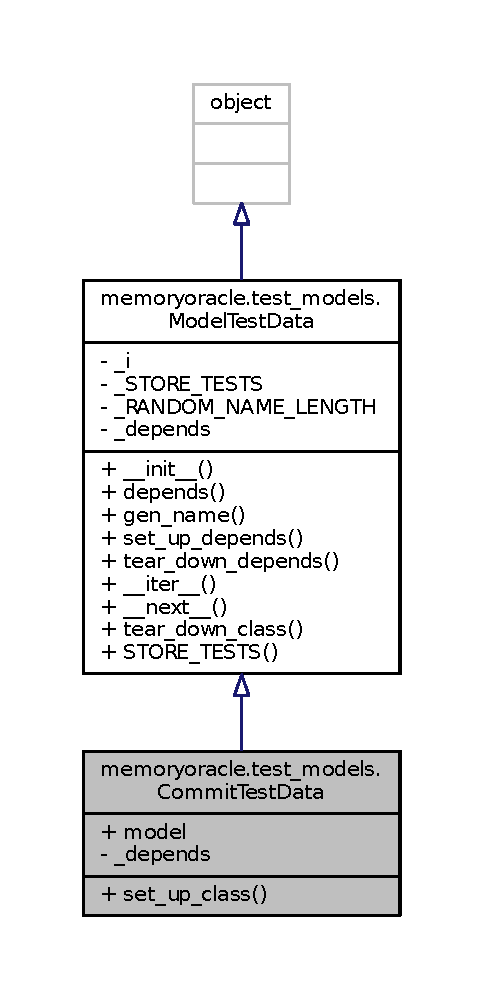
\includegraphics[width=232pt]{classmemoryoracle_1_1test__models_1_1CommitTestData__inherit__graph}
\end{center}
\end{figure}


Collaboration diagram for memoryoracle.\+test\+\_\+models.\+Commit\+Test\+Data\+:\nopagebreak
\begin{figure}[H]
\begin{center}
\leavevmode
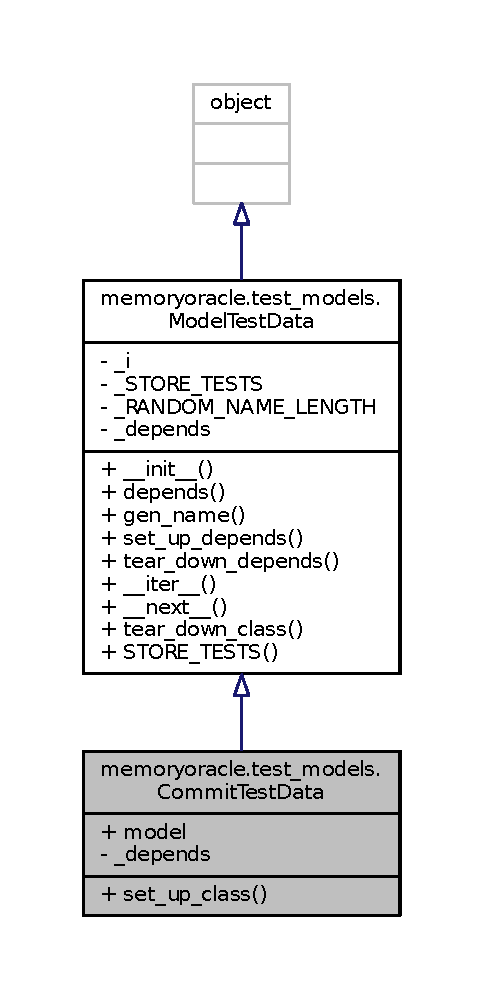
\includegraphics[width=232pt]{classmemoryoracle_1_1test__models_1_1CommitTestData__coll__graph}
\end{center}
\end{figure}
\subsection*{Public Member Functions}
\begin{DoxyCompactItemize}
\item 
def \hyperlink{classmemoryoracle_1_1test__models_1_1CommitTestData_a27d442f991377050929bb9dde59ac3ee}{set\+\_\+up\+\_\+class} (cls)
\end{DoxyCompactItemize}
\subsection*{Static Public Attributes}
\begin{DoxyCompactItemize}
\item 
\hyperlink{classmemoryoracle_1_1test__models_1_1CommitTestData_a1d7335c322637a6769200489933b9338}{model} = \hyperlink{classmemoryoracle_1_1models_1_1Commit}{memoryoracle.\+models.\+Commit}
\end{DoxyCompactItemize}
\subsection*{Static Private Attributes}
\begin{DoxyCompactItemize}
\item 
list \hyperlink{classmemoryoracle_1_1test__models_1_1CommitTestData_ab91d93619fdbadba1be0780696886cdf}{\+\_\+depends} = \mbox{[}\hyperlink{classmemoryoracle_1_1test__models_1_1ProgramTestData}{Program\+Test\+Data}\mbox{]}
\end{DoxyCompactItemize}
\subsection*{Additional Inherited Members}


\subsection{Detailed Description}


Definition at line 114 of file test\+\_\+models.\+py.



\subsection{Member Function Documentation}
\hypertarget{classmemoryoracle_1_1test__models_1_1CommitTestData_a27d442f991377050929bb9dde59ac3ee}{}\index{memoryoracle\+::test\+\_\+models\+::\+Commit\+Test\+Data@{memoryoracle\+::test\+\_\+models\+::\+Commit\+Test\+Data}!set\+\_\+up\+\_\+class@{set\+\_\+up\+\_\+class}}
\index{set\+\_\+up\+\_\+class@{set\+\_\+up\+\_\+class}!memoryoracle\+::test\+\_\+models\+::\+Commit\+Test\+Data@{memoryoracle\+::test\+\_\+models\+::\+Commit\+Test\+Data}}
\subsubsection[{set\+\_\+up\+\_\+class}]{\setlength{\rightskip}{0pt plus 5cm}def memoryoracle.\+test\+\_\+models.\+Commit\+Test\+Data.\+set\+\_\+up\+\_\+class (
\begin{DoxyParamCaption}
\item[{}]{cls}
\end{DoxyParamCaption}
)}\label{classmemoryoracle_1_1test__models_1_1CommitTestData_a27d442f991377050929bb9dde59ac3ee}


Definition at line 121 of file test\+\_\+models.\+py.



References memoryoracle.\+instance.\+x.


\begin{DoxyCode}
121     \textcolor{keyword}{def }\hyperlink{classmemoryoracle_1_1test__models_1_1CommitTestData_a27d442f991377050929bb9dde59ac3ee}{set\_up\_class}(cls):
122         cls.set\_up\_depends()
123         cls.data = \{ x.\_\_name\_\_: \hyperlink{namespacememoryoracle_1_1instance_afe036cc8dc71469743d090c4c80d50c5}{x}() \textcolor{keywordflow}{for} x \textcolor{keywordflow}{in} cls.depends() \}
124         cls.argsList = [
125                 \{
126                     \textcolor{stringliteral}{"name"}: ModelTestData.gen\_name(),
127                     \textcolor{stringliteral}{"id\_program"}: prog,
128                     \textcolor{stringliteral}{"branch\_name"}: ModelTestData.gen\_name(),
129                     \textcolor{stringliteral}{"vcs\_hash"}: ModelTestData.gen\_name()
130                 \} \textcolor{keywordflow}{for} prog \textcolor{keywordflow}{in} cls.data[\textcolor{stringliteral}{"ProgramTestData"}] ]
131         cls.orms = [ cls.model.objects.create(**kwargs) \textcolor{keywordflow}{for} kwargs \textcolor{keywordflow}{in} cls.argsList ]
132 
133 
\end{DoxyCode}


\subsection{Member Data Documentation}
\hypertarget{classmemoryoracle_1_1test__models_1_1CommitTestData_ab91d93619fdbadba1be0780696886cdf}{}\index{memoryoracle\+::test\+\_\+models\+::\+Commit\+Test\+Data@{memoryoracle\+::test\+\_\+models\+::\+Commit\+Test\+Data}!\+\_\+depends@{\+\_\+depends}}
\index{\+\_\+depends@{\+\_\+depends}!memoryoracle\+::test\+\_\+models\+::\+Commit\+Test\+Data@{memoryoracle\+::test\+\_\+models\+::\+Commit\+Test\+Data}}
\subsubsection[{\+\_\+depends}]{\setlength{\rightskip}{0pt plus 5cm}list memoryoracle.\+test\+\_\+models.\+Commit\+Test\+Data.\+\_\+depends = \mbox{[}{\bf Program\+Test\+Data}\mbox{]}\hspace{0.3cm}{\ttfamily [static]}, {\ttfamily [private]}}\label{classmemoryoracle_1_1test__models_1_1CommitTestData_ab91d93619fdbadba1be0780696886cdf}


Definition at line 118 of file test\+\_\+models.\+py.

\hypertarget{classmemoryoracle_1_1test__models_1_1CommitTestData_a1d7335c322637a6769200489933b9338}{}\index{memoryoracle\+::test\+\_\+models\+::\+Commit\+Test\+Data@{memoryoracle\+::test\+\_\+models\+::\+Commit\+Test\+Data}!model@{model}}
\index{model@{model}!memoryoracle\+::test\+\_\+models\+::\+Commit\+Test\+Data@{memoryoracle\+::test\+\_\+models\+::\+Commit\+Test\+Data}}
\subsubsection[{model}]{\setlength{\rightskip}{0pt plus 5cm}memoryoracle.\+test\+\_\+models.\+Commit\+Test\+Data.\+model = {\bf memoryoracle.\+models.\+Commit}\hspace{0.3cm}{\ttfamily [static]}}\label{classmemoryoracle_1_1test__models_1_1CommitTestData_a1d7335c322637a6769200489933b9338}


Definition at line 116 of file test\+\_\+models.\+py.



The documentation for this class was generated from the following file\+:\begin{DoxyCompactItemize}
\item 
memoryoracle/\hyperlink{test__models_8py}{test\+\_\+models.\+py}\end{DoxyCompactItemize}

\hypertarget{classmemoryoracle_1_1instance_1_1ConstDecorator}{}\section{memoryoracle.\+instance.\+Const\+Decorator Class Reference}
\label{classmemoryoracle_1_1instance_1_1ConstDecorator}\index{memoryoracle.\+instance.\+Const\+Decorator@{memoryoracle.\+instance.\+Const\+Decorator}}


Inheritance diagram for memoryoracle.\+instance.\+Const\+Decorator\+:
\nopagebreak
\begin{figure}[H]
\begin{center}
\leavevmode
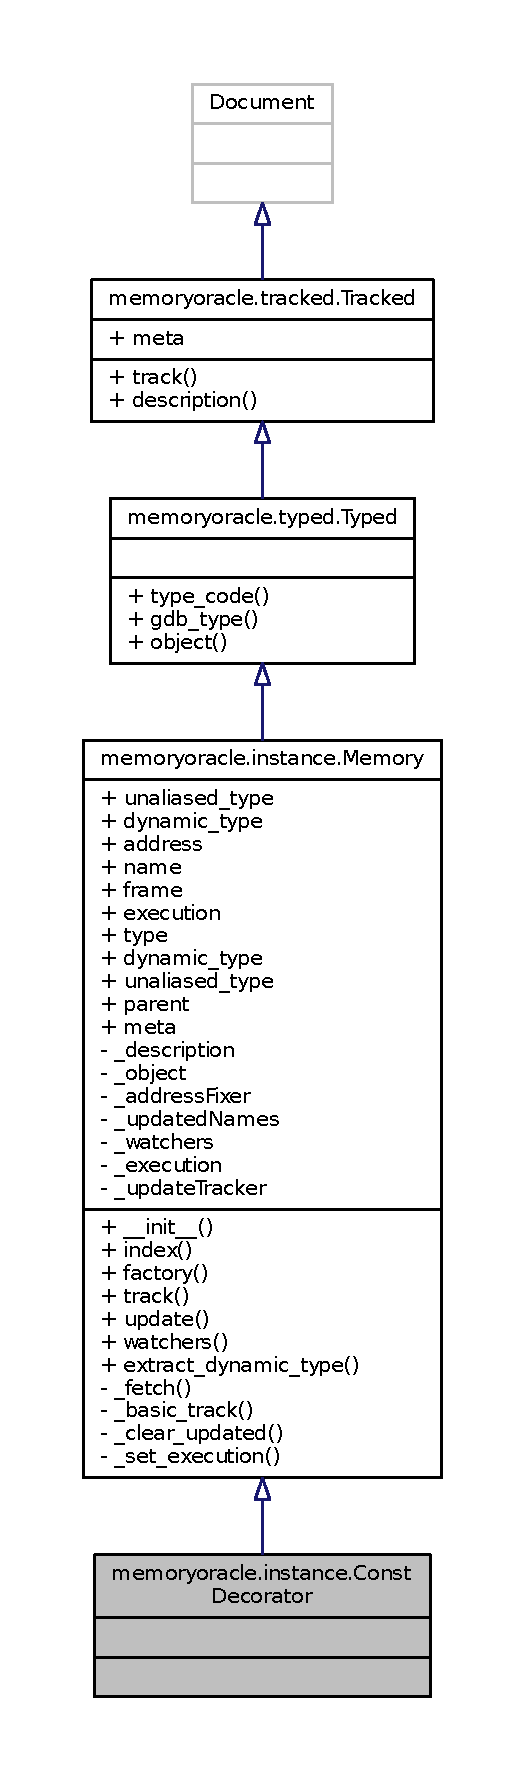
\includegraphics[height=550pt]{classmemoryoracle_1_1instance_1_1ConstDecorator__inherit__graph}
\end{center}
\end{figure}


Collaboration diagram for memoryoracle.\+instance.\+Const\+Decorator\+:
\nopagebreak
\begin{figure}[H]
\begin{center}
\leavevmode
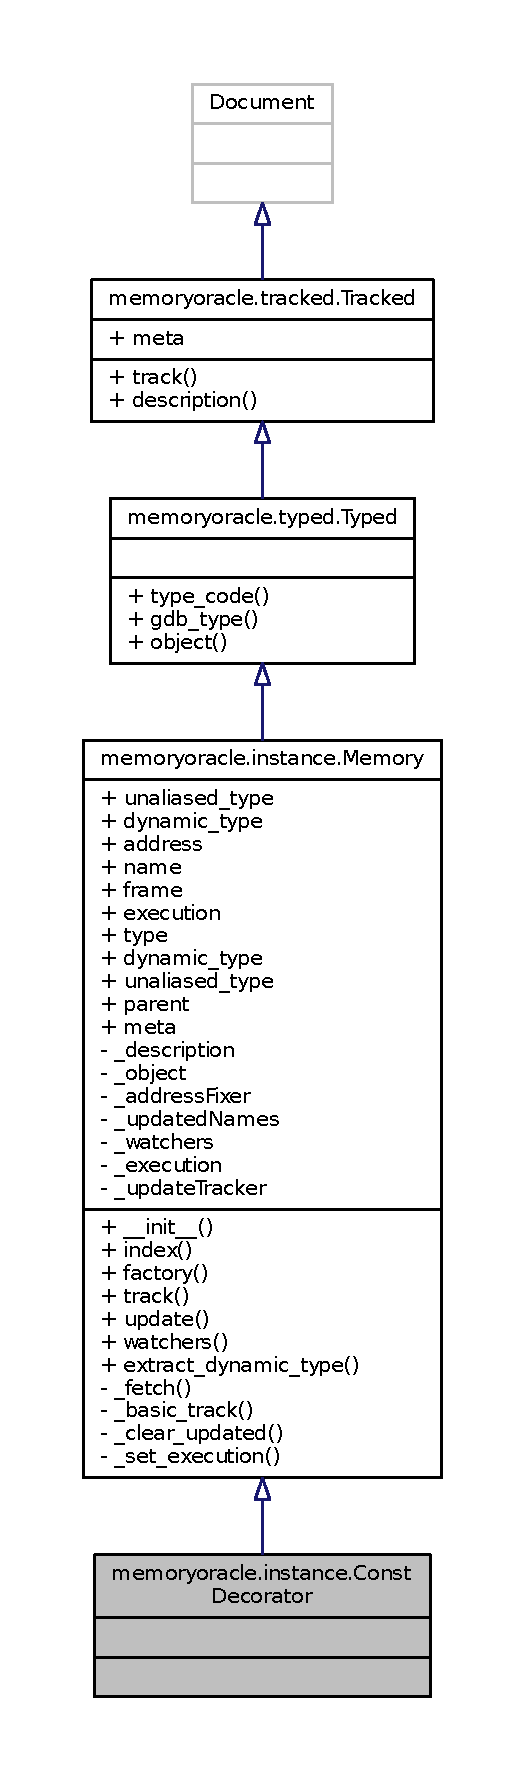
\includegraphics[height=550pt]{classmemoryoracle_1_1instance_1_1ConstDecorator__coll__graph}
\end{center}
\end{figure}
\subsection*{Additional Inherited Members}


\subsection{Detailed Description}
\begin{DoxyVerb}*Decorator* class to decorate an addressable as being marked const.
\end{DoxyVerb}
 

Definition at line 465 of file instance.\+py.



The documentation for this class was generated from the following file\+:\begin{DoxyCompactItemize}
\item 
memoryoracle/\hyperlink{instance_8py}{instance.\+py}\end{DoxyCompactItemize}

\hypertarget{classmemoryoracle_1_1container_1_1Container}{}\section{memoryoracle.\+container.\+Container Class Reference}
\label{classmemoryoracle_1_1container_1_1Container}\index{memoryoracle.\+container.\+Container@{memoryoracle.\+container.\+Container}}


Inheritance diagram for memoryoracle.\+container.\+Container\+:\nopagebreak
\begin{figure}[H]
\begin{center}
\leavevmode
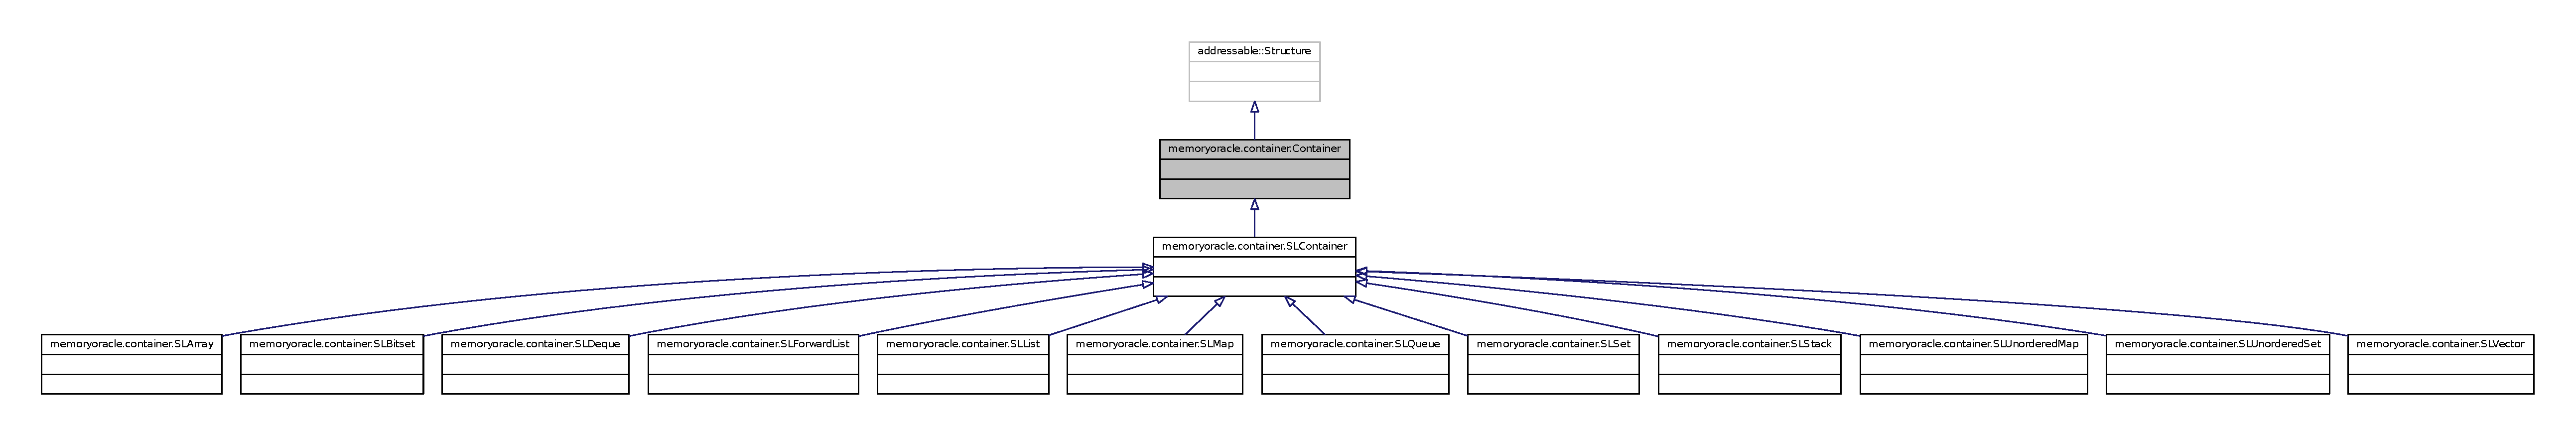
\includegraphics[width=350pt]{classmemoryoracle_1_1container_1_1Container__inherit__graph}
\end{center}
\end{figure}


Collaboration diagram for memoryoracle.\+container.\+Container\+:\nopagebreak
\begin{figure}[H]
\begin{center}
\leavevmode
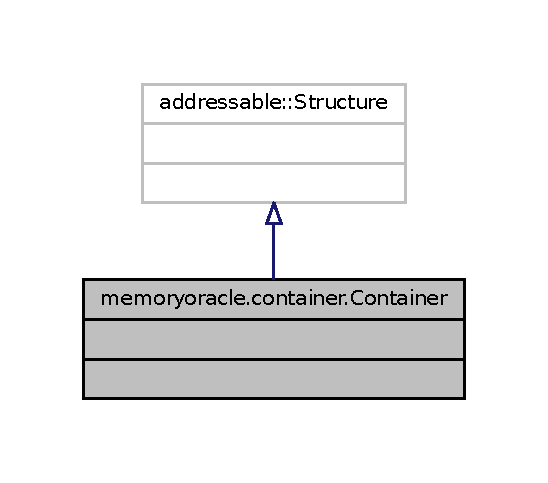
\includegraphics[width=263pt]{classmemoryoracle_1_1container_1_1Container__coll__graph}
\end{center}
\end{figure}


\subsection{Detailed Description}
\begin{DoxyVerb}*Abstract* class to represent a C++ container.

This is mostly intended to help correct rendering for
standard library containers, but should be helpful for
user defined containers as well.
\end{DoxyVerb}
 

Definition at line 6 of file container.\+py.



The documentation for this class was generated from the following file\+:\begin{DoxyCompactItemize}
\item 
memoryoracle/\hyperlink{container_8py}{container.\+py}\end{DoxyCompactItemize}

\hypertarget{classmemoryoracle_1_1models_1_1Typed_1_1DataError}{}\section{memoryoracle.\+models.\+Typed.\+Data\+Error Class Reference}
\label{classmemoryoracle_1_1models_1_1Typed_1_1DataError}\index{memoryoracle.\+models.\+Typed.\+Data\+Error@{memoryoracle.\+models.\+Typed.\+Data\+Error}}


Inheritance diagram for memoryoracle.\+models.\+Typed.\+Data\+Error\+:\nopagebreak
\begin{figure}[H]
\begin{center}
\leavevmode
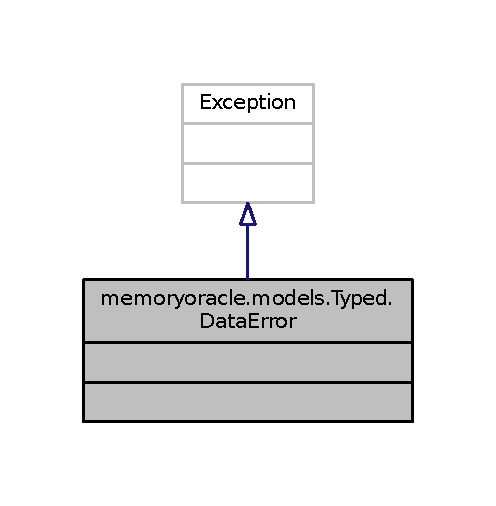
\includegraphics[width=238pt]{classmemoryoracle_1_1models_1_1Typed_1_1DataError__inherit__graph}
\end{center}
\end{figure}


Collaboration diagram for memoryoracle.\+models.\+Typed.\+Data\+Error\+:\nopagebreak
\begin{figure}[H]
\begin{center}
\leavevmode
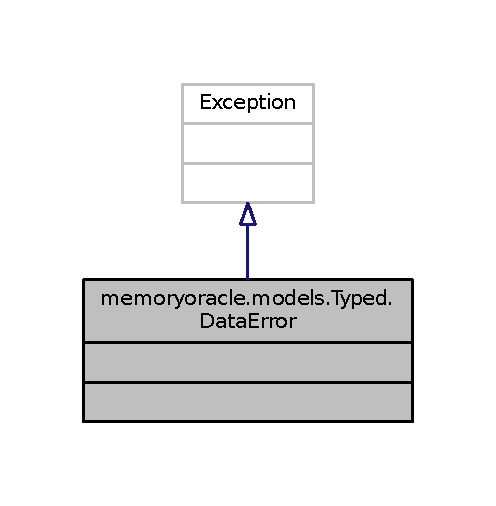
\includegraphics[width=238pt]{classmemoryoracle_1_1models_1_1Typed_1_1DataError__coll__graph}
\end{center}
\end{figure}


\subsection{Detailed Description}


Definition at line 94 of file models.\+py.



The documentation for this class was generated from the following file\+:\begin{DoxyCompactItemize}
\item 
memoryoracle/\hyperlink{models_8py}{models.\+py}\end{DoxyCompactItemize}

\hypertarget{classmemoryoracle_1_1descriptions_1_1Description}{}\section{memoryoracle.\+descriptions.\+Description Class Reference}
\label{classmemoryoracle_1_1descriptions_1_1Description}\index{memoryoracle.\+descriptions.\+Description@{memoryoracle.\+descriptions.\+Description}}


Inheritance diagram for memoryoracle.\+descriptions.\+Description\+:
\nopagebreak
\begin{figure}[H]
\begin{center}
\leavevmode
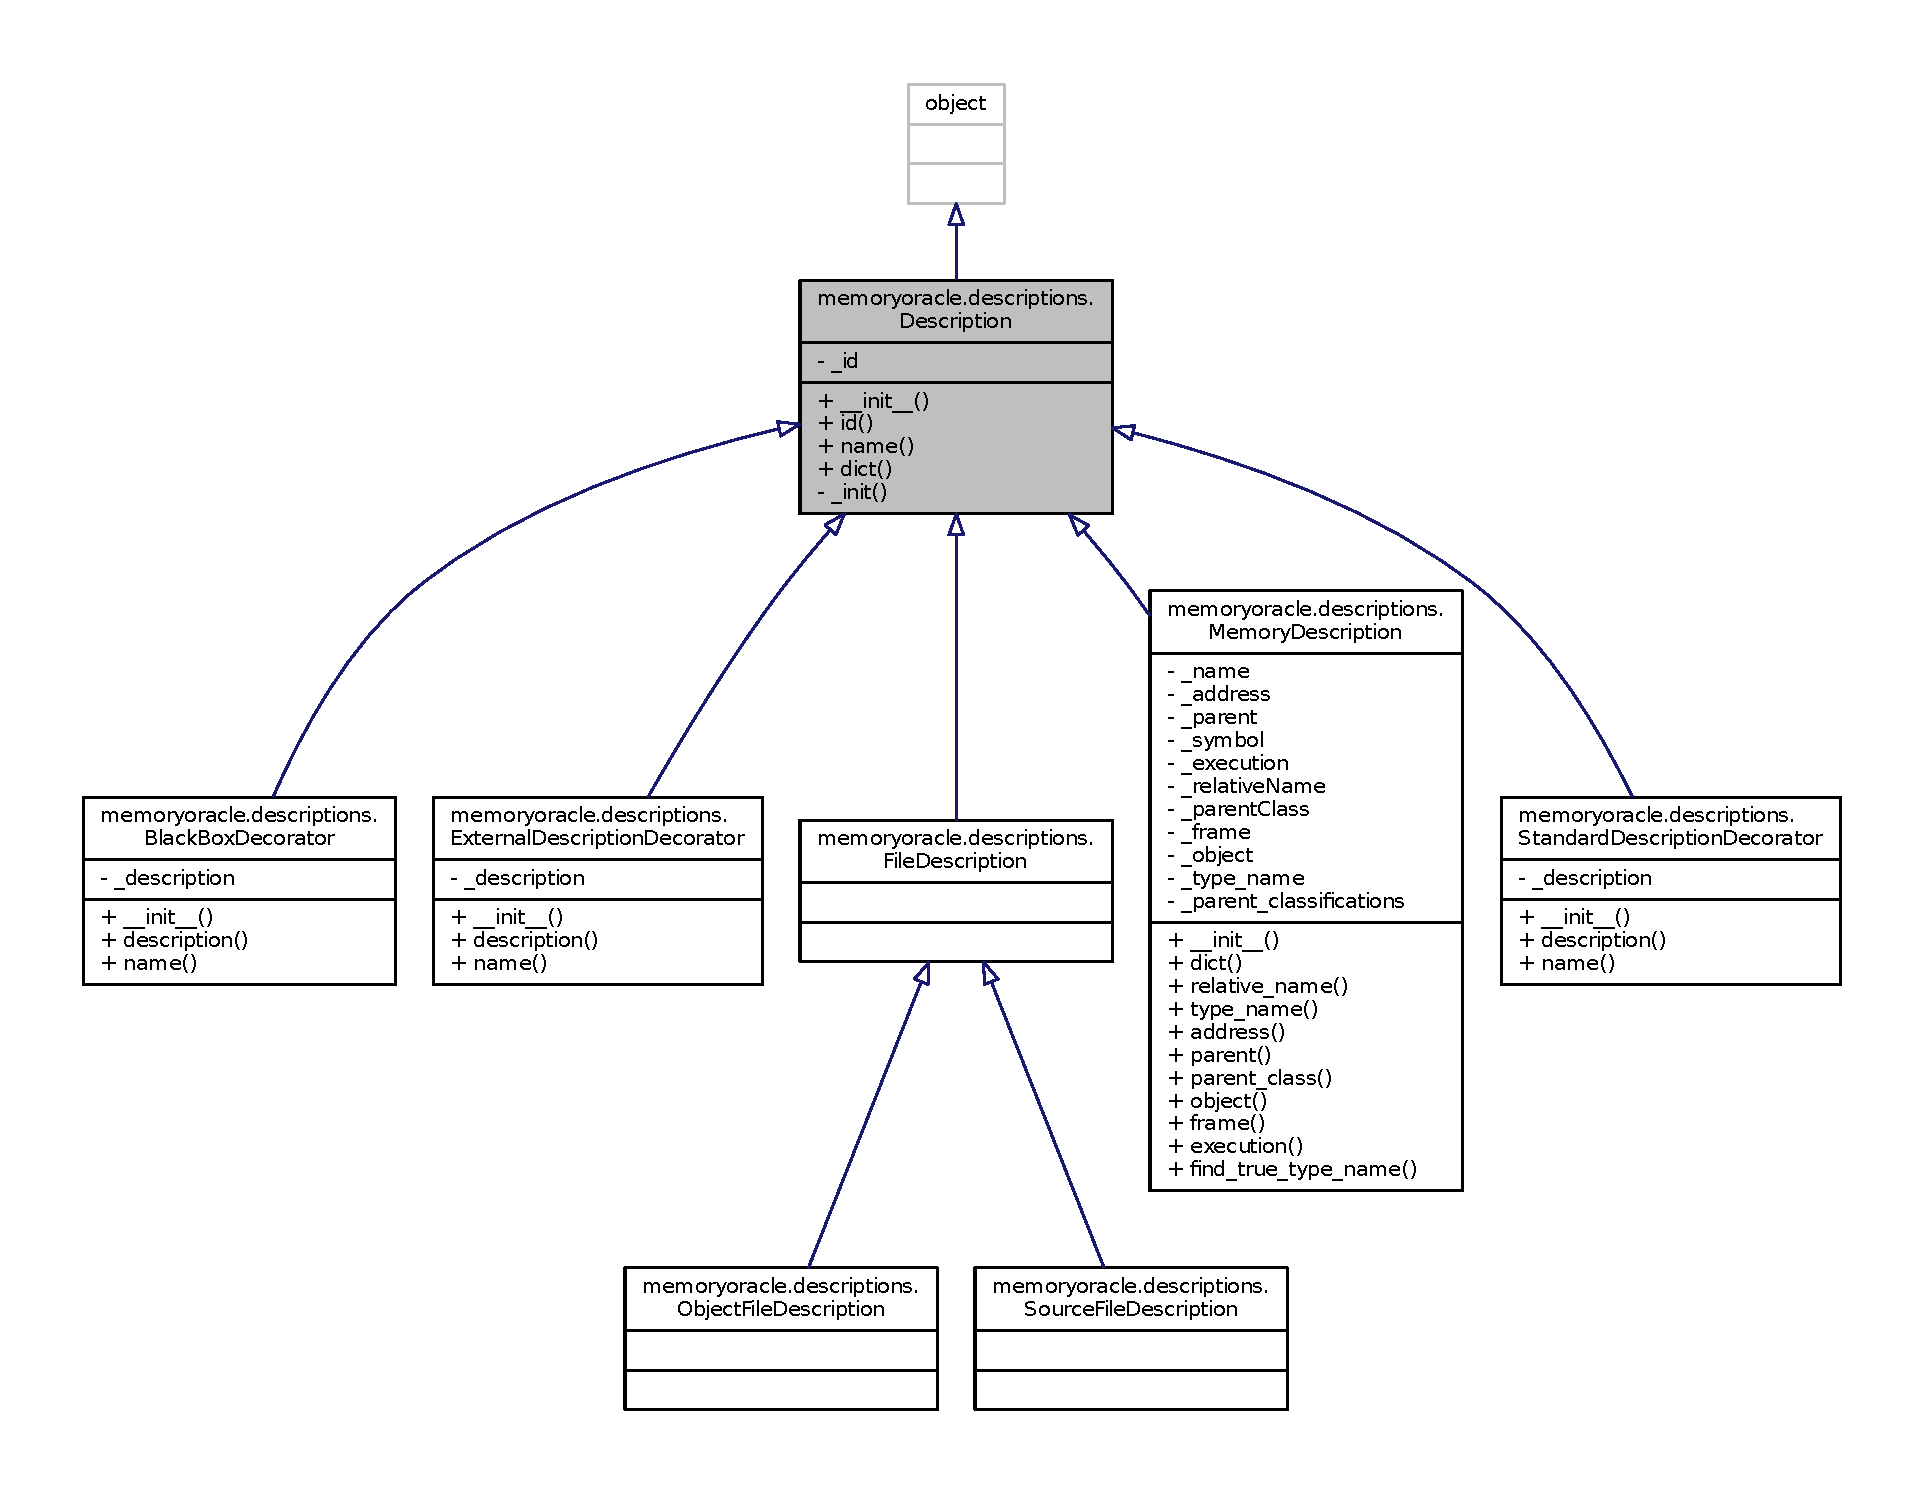
\includegraphics[width=350pt]{classmemoryoracle_1_1descriptions_1_1Description__inherit__graph}
\end{center}
\end{figure}


Collaboration diagram for memoryoracle.\+descriptions.\+Description\+:\nopagebreak
\begin{figure}[H]
\begin{center}
\leavevmode
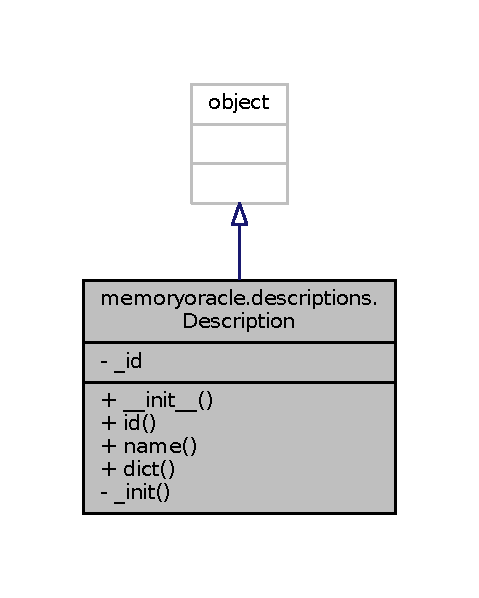
\includegraphics[width=230pt]{classmemoryoracle_1_1descriptions_1_1Description__coll__graph}
\end{center}
\end{figure}
\subsection*{Public Member Functions}
\begin{DoxyCompactItemize}
\item 
def \hyperlink{classmemoryoracle_1_1descriptions_1_1Description_a4fb6dc4bf9be65d6d1b135a9af46af38}{\+\_\+\+\_\+init\+\_\+\+\_\+} (self, args, kwargs)
\item 
def \hyperlink{classmemoryoracle_1_1descriptions_1_1Description_a793ffb6975ee167869a1f475b1748769}{id} (self)
\item 
def \hyperlink{classmemoryoracle_1_1descriptions_1_1Description_a4b27c3ae1ef0ab35ec0f990fa553b8b3}{name} (self)
\item 
def \hyperlink{classmemoryoracle_1_1descriptions_1_1Description_ab09bce45e6b9a038366ef720a5253506}{dict} (self)
\end{DoxyCompactItemize}
\subsection*{Private Member Functions}
\begin{DoxyCompactItemize}
\item 
def \hyperlink{classmemoryoracle_1_1descriptions_1_1Description_a61b082efab73e7121ad7321bd5d21b84}{\+\_\+init} (self)
\end{DoxyCompactItemize}
\subsection*{Private Attributes}
\begin{DoxyCompactItemize}
\item 
\hyperlink{classmemoryoracle_1_1descriptions_1_1Description_a75740a1e65e4640ddd011d2c98aad5c3}{\+\_\+id}
\end{DoxyCompactItemize}


\subsection{Detailed Description}
\begin{DoxyVerb}*Abstract* Description class.

This is the superclass of all the different kinds of
descriptions used by the subclasses of Tracked.
\end{DoxyVerb}
 

Definition at line 12 of file descriptions.\+py.



\subsection{Constructor \& Destructor Documentation}
\hypertarget{classmemoryoracle_1_1descriptions_1_1Description_a4fb6dc4bf9be65d6d1b135a9af46af38}{}\index{memoryoracle\+::descriptions\+::\+Description@{memoryoracle\+::descriptions\+::\+Description}!\+\_\+\+\_\+init\+\_\+\+\_\+@{\+\_\+\+\_\+init\+\_\+\+\_\+}}
\index{\+\_\+\+\_\+init\+\_\+\+\_\+@{\+\_\+\+\_\+init\+\_\+\+\_\+}!memoryoracle\+::descriptions\+::\+Description@{memoryoracle\+::descriptions\+::\+Description}}
\subsubsection[{\+\_\+\+\_\+init\+\_\+\+\_\+}]{\setlength{\rightskip}{0pt plus 5cm}def memoryoracle.\+descriptions.\+Description.\+\_\+\+\_\+init\+\_\+\+\_\+ (
\begin{DoxyParamCaption}
\item[{}]{self, }
\item[{}]{args, }
\item[{}]{kwargs}
\end{DoxyParamCaption}
)}\label{classmemoryoracle_1_1descriptions_1_1Description_a4fb6dc4bf9be65d6d1b135a9af46af38}


Definition at line 23 of file descriptions.\+py.


\begin{DoxyCode}
23     \textcolor{keyword}{def }\hyperlink{classmemoryoracle_1_1descriptions_1_1Description_a4fb6dc4bf9be65d6d1b135a9af46af38}{\_\_init\_\_}(self, *args, **kwargs):
24         \textcolor{keywordflow}{raise} NotImplementedError(
25                 \textcolor{stringliteral}{"Attempt to instiante abstract class"});
26 
\end{DoxyCode}


\subsection{Member Function Documentation}
\hypertarget{classmemoryoracle_1_1descriptions_1_1Description_a61b082efab73e7121ad7321bd5d21b84}{}\index{memoryoracle\+::descriptions\+::\+Description@{memoryoracle\+::descriptions\+::\+Description}!\+\_\+init@{\+\_\+init}}
\index{\+\_\+init@{\+\_\+init}!memoryoracle\+::descriptions\+::\+Description@{memoryoracle\+::descriptions\+::\+Description}}
\subsubsection[{\+\_\+init}]{\setlength{\rightskip}{0pt plus 5cm}def memoryoracle.\+descriptions.\+Description.\+\_\+init (
\begin{DoxyParamCaption}
\item[{}]{self}
\end{DoxyParamCaption}
)\hspace{0.3cm}{\ttfamily [private]}}\label{classmemoryoracle_1_1descriptions_1_1Description_a61b082efab73e7121ad7321bd5d21b84}


Definition at line 20 of file descriptions.\+py.


\begin{DoxyCode}
20     \textcolor{keyword}{def }\hyperlink{classmemoryoracle_1_1descriptions_1_1Description_a61b082efab73e7121ad7321bd5d21b84}{\_init}(self):
21         self.\hyperlink{classmemoryoracle_1_1descriptions_1_1Description_a75740a1e65e4640ddd011d2c98aad5c3}{\_id} = str(uuid())
22 
\end{DoxyCode}
\hypertarget{classmemoryoracle_1_1descriptions_1_1Description_ab09bce45e6b9a038366ef720a5253506}{}\index{memoryoracle\+::descriptions\+::\+Description@{memoryoracle\+::descriptions\+::\+Description}!dict@{dict}}
\index{dict@{dict}!memoryoracle\+::descriptions\+::\+Description@{memoryoracle\+::descriptions\+::\+Description}}
\subsubsection[{dict}]{\setlength{\rightskip}{0pt plus 5cm}def memoryoracle.\+descriptions.\+Description.\+dict (
\begin{DoxyParamCaption}
\item[{}]{self}
\end{DoxyParamCaption}
)}\label{classmemoryoracle_1_1descriptions_1_1Description_ab09bce45e6b9a038366ef720a5253506}


Definition at line 36 of file descriptions.\+py.


\begin{DoxyCode}
36     \textcolor{keyword}{def }\hyperlink{classmemoryoracle_1_1descriptions_1_1Description_ab09bce45e6b9a038366ef720a5253506}{dict}(self):
37         \textcolor{keywordflow}{raise} NotImplementedError(
38                 \textcolor{stringliteral}{"Can not transform abstract class Description to dict"})
39 
40 
\end{DoxyCode}
\hypertarget{classmemoryoracle_1_1descriptions_1_1Description_a793ffb6975ee167869a1f475b1748769}{}\index{memoryoracle\+::descriptions\+::\+Description@{memoryoracle\+::descriptions\+::\+Description}!id@{id}}
\index{id@{id}!memoryoracle\+::descriptions\+::\+Description@{memoryoracle\+::descriptions\+::\+Description}}
\subsubsection[{id}]{\setlength{\rightskip}{0pt plus 5cm}def memoryoracle.\+descriptions.\+Description.\+id (
\begin{DoxyParamCaption}
\item[{}]{self}
\end{DoxyParamCaption}
)}\label{classmemoryoracle_1_1descriptions_1_1Description_a793ffb6975ee167869a1f475b1748769}


Definition at line 28 of file descriptions.\+py.



References memoryoracle.\+descriptions.\+Description.\+\_\+id.


\begin{DoxyCode}
28     \textcolor{keyword}{def }\hyperlink{classmemoryoracle_1_1descriptions_1_1Description_a793ffb6975ee167869a1f475b1748769}{id}(self):
29         \textcolor{keywordflow}{return} self.\hyperlink{classmemoryoracle_1_1descriptions_1_1Description_a75740a1e65e4640ddd011d2c98aad5c3}{\_id}
30 
\end{DoxyCode}
\hypertarget{classmemoryoracle_1_1descriptions_1_1Description_a4b27c3ae1ef0ab35ec0f990fa553b8b3}{}\index{memoryoracle\+::descriptions\+::\+Description@{memoryoracle\+::descriptions\+::\+Description}!name@{name}}
\index{name@{name}!memoryoracle\+::descriptions\+::\+Description@{memoryoracle\+::descriptions\+::\+Description}}
\subsubsection[{name}]{\setlength{\rightskip}{0pt plus 5cm}def memoryoracle.\+descriptions.\+Description.\+name (
\begin{DoxyParamCaption}
\item[{}]{self}
\end{DoxyParamCaption}
)}\label{classmemoryoracle_1_1descriptions_1_1Description_a4b27c3ae1ef0ab35ec0f990fa553b8b3}


Definition at line 32 of file descriptions.\+py.



References memoryoracle.\+descriptions.\+Memory\+Description.\+\_\+name.



Referenced by memoryoracle.\+descriptions.\+Memory\+Description.\+dict().


\begin{DoxyCode}
32     \textcolor{keyword}{def }\hyperlink{classmemoryoracle_1_1descriptions_1_1Description_a4b27c3ae1ef0ab35ec0f990fa553b8b3}{name}(self):
33         \textcolor{keywordflow}{return} self.\_name
34 
\end{DoxyCode}


Here is the caller graph for this function\+:
\nopagebreak
\begin{figure}[H]
\begin{center}
\leavevmode
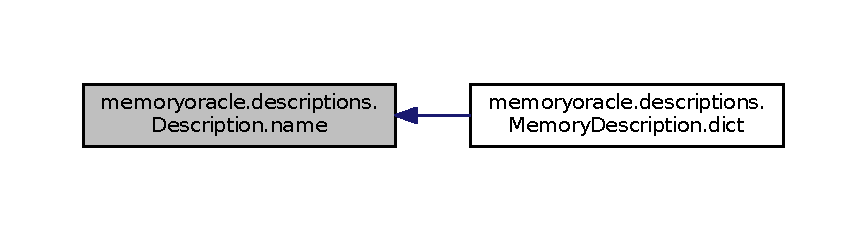
\includegraphics[width=350pt]{classmemoryoracle_1_1descriptions_1_1Description_a4b27c3ae1ef0ab35ec0f990fa553b8b3_icgraph}
\end{center}
\end{figure}




\subsection{Member Data Documentation}
\hypertarget{classmemoryoracle_1_1descriptions_1_1Description_a75740a1e65e4640ddd011d2c98aad5c3}{}\index{memoryoracle\+::descriptions\+::\+Description@{memoryoracle\+::descriptions\+::\+Description}!\+\_\+id@{\+\_\+id}}
\index{\+\_\+id@{\+\_\+id}!memoryoracle\+::descriptions\+::\+Description@{memoryoracle\+::descriptions\+::\+Description}}
\subsubsection[{\+\_\+id}]{\setlength{\rightskip}{0pt plus 5cm}memoryoracle.\+descriptions.\+Description.\+\_\+id\hspace{0.3cm}{\ttfamily [private]}}\label{classmemoryoracle_1_1descriptions_1_1Description_a75740a1e65e4640ddd011d2c98aad5c3}


Definition at line 21 of file descriptions.\+py.



Referenced by memoryoracle.\+descriptions.\+Description.\+id().



The documentation for this class was generated from the following file\+:\begin{DoxyCompactItemize}
\item 
memoryoracle/\hyperlink{descriptions_8py}{descriptions.\+py}\end{DoxyCompactItemize}

\hypertarget{classmemoryoracle_1_1models_1_1Typed_1_1DetectionError}{}\section{memoryoracle.\+models.\+Typed.\+Detection\+Error Class Reference}
\label{classmemoryoracle_1_1models_1_1Typed_1_1DetectionError}\index{memoryoracle.\+models.\+Typed.\+Detection\+Error@{memoryoracle.\+models.\+Typed.\+Detection\+Error}}


Inheritance diagram for memoryoracle.\+models.\+Typed.\+Detection\+Error\+:\nopagebreak
\begin{figure}[H]
\begin{center}
\leavevmode
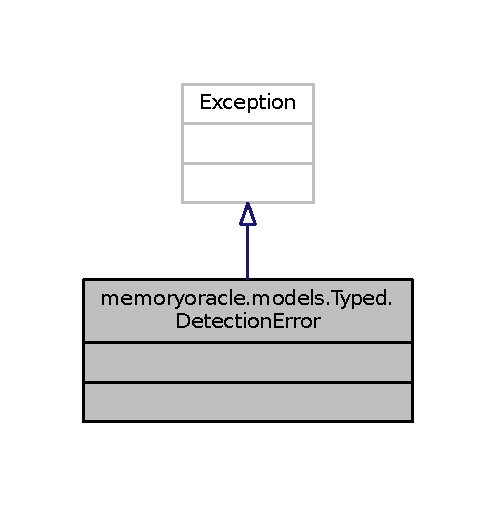
\includegraphics[width=238pt]{classmemoryoracle_1_1models_1_1Typed_1_1DetectionError__inherit__graph}
\end{center}
\end{figure}


Collaboration diagram for memoryoracle.\+models.\+Typed.\+Detection\+Error\+:\nopagebreak
\begin{figure}[H]
\begin{center}
\leavevmode
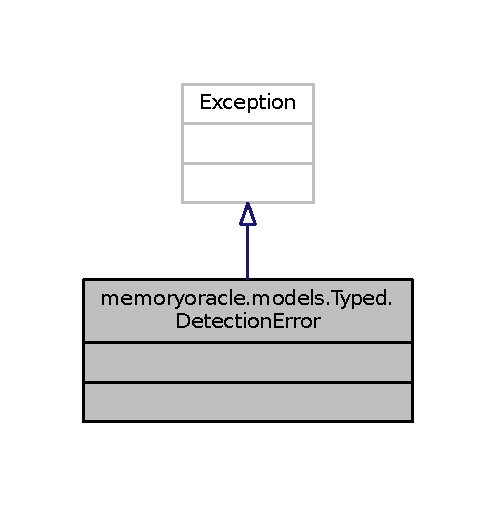
\includegraphics[width=238pt]{classmemoryoracle_1_1models_1_1Typed_1_1DetectionError__coll__graph}
\end{center}
\end{figure}


\subsection{Detailed Description}


Definition at line 91 of file models.\+py.



The documentation for this class was generated from the following file\+:\begin{DoxyCompactItemize}
\item 
memoryoracle/\hyperlink{models_8py}{models.\+py}\end{DoxyCompactItemize}

\hypertarget{classmemoryoracle_1_1instance_1_1Memory_1_1DuplicateAddress}{}\section{memoryoracle.\+instance.\+Memory.\+Duplicate\+Address Class Reference}
\label{classmemoryoracle_1_1instance_1_1Memory_1_1DuplicateAddress}\index{memoryoracle.\+instance.\+Memory.\+Duplicate\+Address@{memoryoracle.\+instance.\+Memory.\+Duplicate\+Address}}


Inheritance diagram for memoryoracle.\+instance.\+Memory.\+Duplicate\+Address\+:
\nopagebreak
\begin{figure}[H]
\begin{center}
\leavevmode
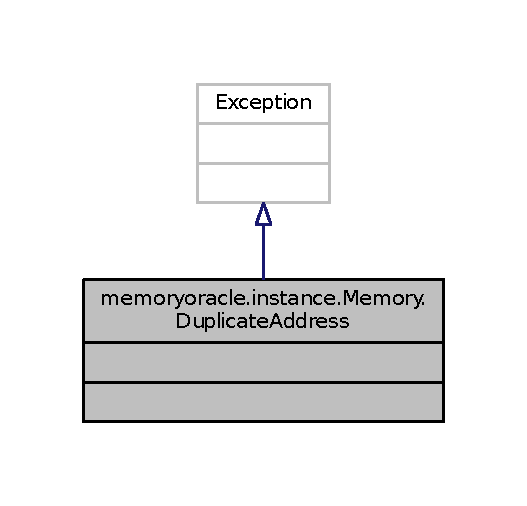
\includegraphics[width=253pt]{classmemoryoracle_1_1instance_1_1Memory_1_1DuplicateAddress__inherit__graph}
\end{center}
\end{figure}


Collaboration diagram for memoryoracle.\+instance.\+Memory.\+Duplicate\+Address\+:
\nopagebreak
\begin{figure}[H]
\begin{center}
\leavevmode
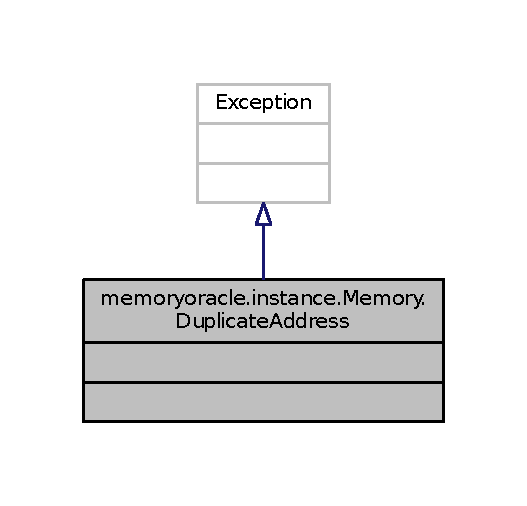
\includegraphics[width=253pt]{classmemoryoracle_1_1instance_1_1Memory_1_1DuplicateAddress__coll__graph}
\end{center}
\end{figure}


\subsection{Detailed Description}


Definition at line 62 of file instance.\+py.



The documentation for this class was generated from the following file\+:\begin{DoxyCompactItemize}
\item 
memoryoracle/\hyperlink{instance_8py}{instance.\+py}\end{DoxyCompactItemize}

\hypertarget{classmemoryoracle_1_1symbol_1_1Enum}{}\section{memoryoracle.\+symbol.\+Enum Class Reference}
\label{classmemoryoracle_1_1symbol_1_1Enum}\index{memoryoracle.\+symbol.\+Enum@{memoryoracle.\+symbol.\+Enum}}


Inheritance diagram for memoryoracle.\+symbol.\+Enum\+:
\nopagebreak
\begin{figure}[H]
\begin{center}
\leavevmode
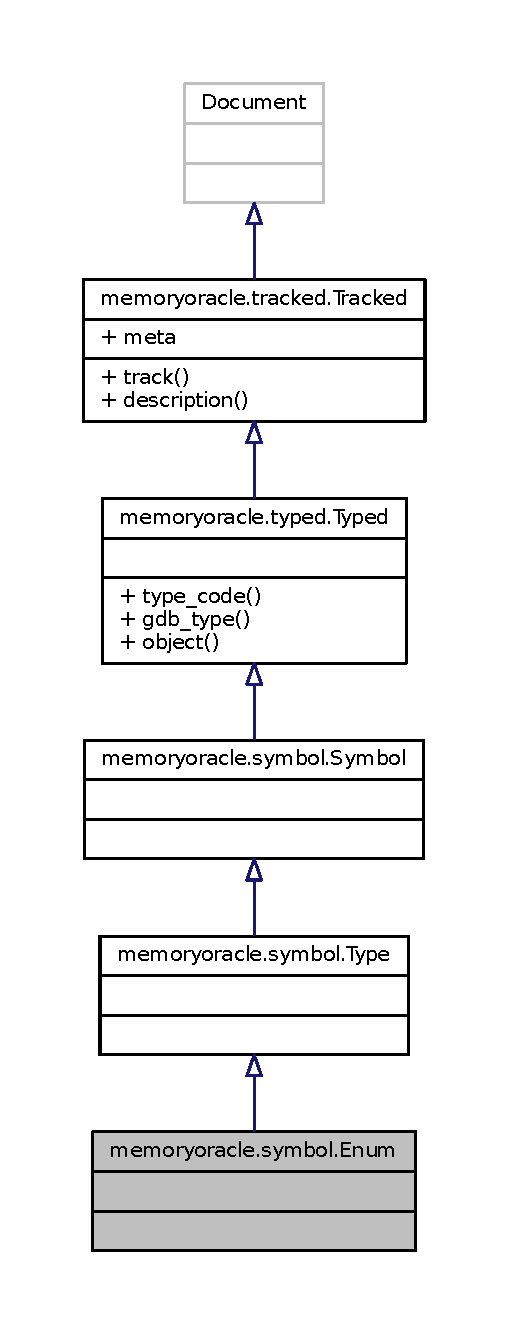
\includegraphics[height=550pt]{classmemoryoracle_1_1symbol_1_1Enum__inherit__graph}
\end{center}
\end{figure}


Collaboration diagram for memoryoracle.\+symbol.\+Enum\+:
\nopagebreak
\begin{figure}[H]
\begin{center}
\leavevmode
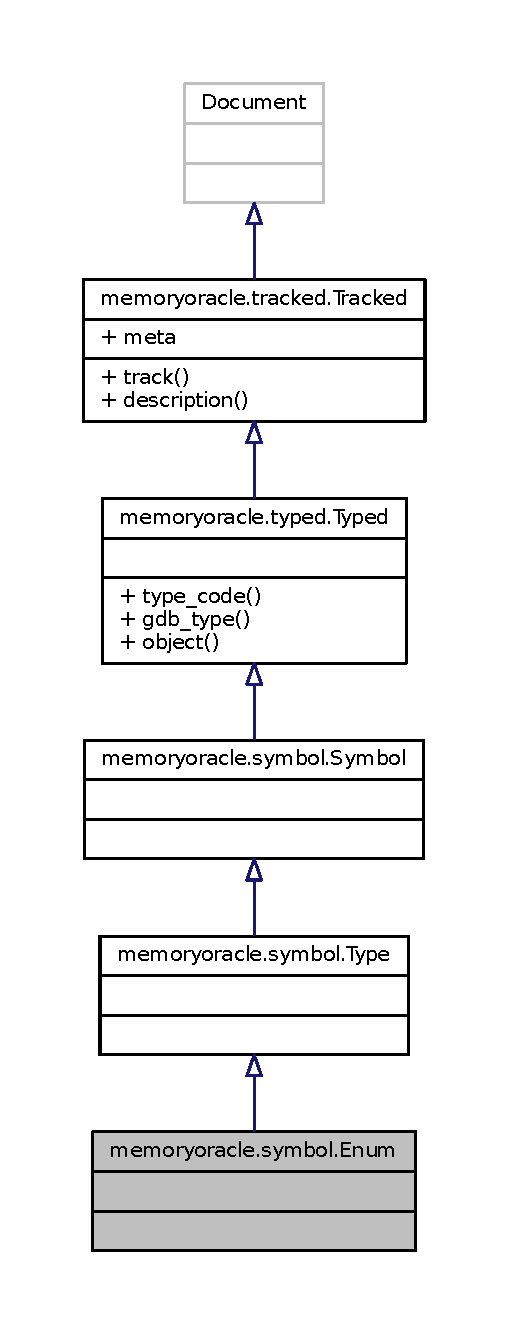
\includegraphics[height=550pt]{classmemoryoracle_1_1symbol_1_1Enum__coll__graph}
\end{center}
\end{figure}
\subsection*{Additional Inherited Members}


\subsection{Detailed Description}


Definition at line 52 of file symbol.\+py.



The documentation for this class was generated from the following file\+:\begin{DoxyCompactItemize}
\item 
memoryoracle/\hyperlink{symbol_8py}{symbol.\+py}\end{DoxyCompactItemize}

\hypertarget{classmemoryoracle_1_1execution_1_1Executable}{}\section{memoryoracle.\+execution.\+Executable Class Reference}
\label{classmemoryoracle_1_1execution_1_1Executable}\index{memoryoracle.\+execution.\+Executable@{memoryoracle.\+execution.\+Executable}}


Inheritance diagram for memoryoracle.\+execution.\+Executable\+:\nopagebreak
\begin{figure}[H]
\begin{center}
\leavevmode
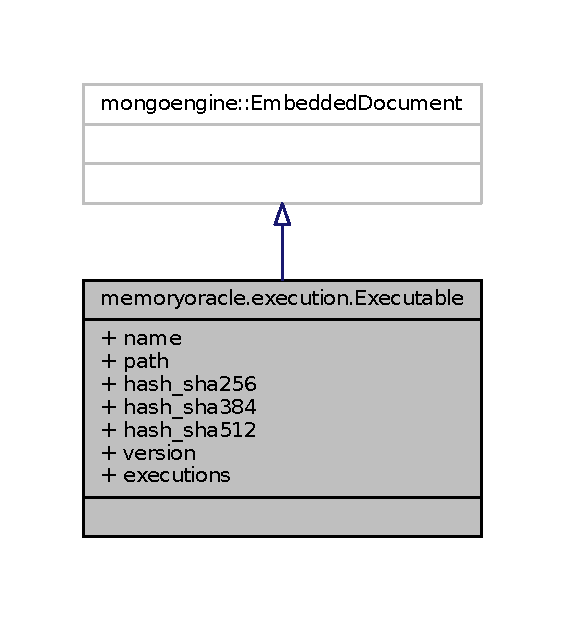
\includegraphics[width=271pt]{classmemoryoracle_1_1execution_1_1Executable__inherit__graph}
\end{center}
\end{figure}


Collaboration diagram for memoryoracle.\+execution.\+Executable\+:\nopagebreak
\begin{figure}[H]
\begin{center}
\leavevmode
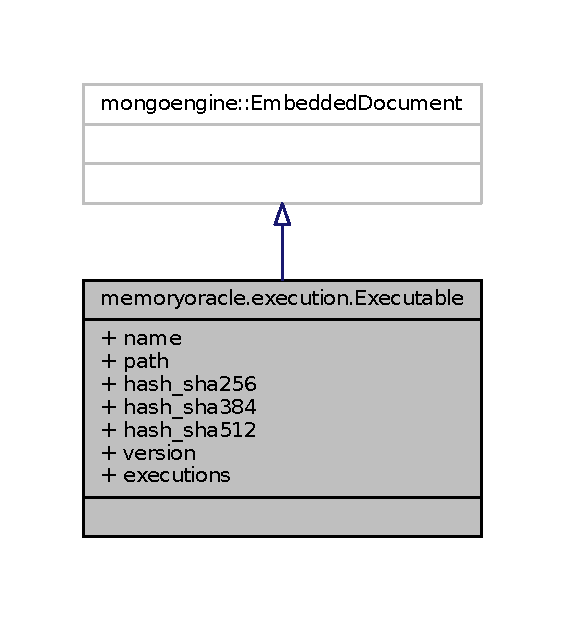
\includegraphics[width=271pt]{classmemoryoracle_1_1execution_1_1Executable__coll__graph}
\end{center}
\end{figure}
\subsection*{Static Public Attributes}
\begin{DoxyCompactItemize}
\item 
tuple \hyperlink{classmemoryoracle_1_1execution_1_1Executable_a52369e49bc4e8eea72149649accd2650}{name} = mongoengine.\+String\+Field()
\item 
tuple \hyperlink{classmemoryoracle_1_1execution_1_1Executable_a783237790a0dde89a8d29c2c56983303}{path} = mongoengine.\+String\+Field()
\item 
tuple \hyperlink{classmemoryoracle_1_1execution_1_1Executable_af209643fc8bba25bb96282463a2274d7}{hash\+\_\+sha256} = mongoengine.\+String\+Field()
\item 
tuple \hyperlink{classmemoryoracle_1_1execution_1_1Executable_aaa57eabb3dec08378d484a6f7f519fe2}{hash\+\_\+sha384} = mongoengine.\+String\+Field()
\item 
tuple \hyperlink{classmemoryoracle_1_1execution_1_1Executable_afd44dfe3eb583f3c185b66a619e7923b}{hash\+\_\+sha512} = mongoengine.\+String\+Field()
\item 
tuple \hyperlink{classmemoryoracle_1_1execution_1_1Executable_a7ef44544b8c9b148bf066357bfa37f92}{version} = mongoengine.\+String\+Field()
\item 
tuple \hyperlink{classmemoryoracle_1_1execution_1_1Executable_a445e571531520c3ec32754988b4d7ee6}{executions} = mongoengine.\+List\+Field(mongoengine.\+Reference\+Field(\hyperlink{classmemoryoracle_1_1execution_1_1Execution}{Execution}))
\end{DoxyCompactItemize}


\subsection{Detailed Description}
\begin{DoxyVerb}*Concrete* class representing a executable file generated by running
build on a commit
\end{DoxyVerb}
 

Definition at line 34 of file execution.\+py.



\subsection{Member Data Documentation}
\hypertarget{classmemoryoracle_1_1execution_1_1Executable_a445e571531520c3ec32754988b4d7ee6}{}\index{memoryoracle\+::execution\+::\+Executable@{memoryoracle\+::execution\+::\+Executable}!executions@{executions}}
\index{executions@{executions}!memoryoracle\+::execution\+::\+Executable@{memoryoracle\+::execution\+::\+Executable}}
\subsubsection[{executions}]{\setlength{\rightskip}{0pt plus 5cm}tuple memoryoracle.\+execution.\+Executable.\+executions = mongoengine.\+List\+Field(mongoengine.\+Reference\+Field({\bf Execution}))\hspace{0.3cm}{\ttfamily [static]}}\label{classmemoryoracle_1_1execution_1_1Executable_a445e571531520c3ec32754988b4d7ee6}


Definition at line 45 of file execution.\+py.

\hypertarget{classmemoryoracle_1_1execution_1_1Executable_af209643fc8bba25bb96282463a2274d7}{}\index{memoryoracle\+::execution\+::\+Executable@{memoryoracle\+::execution\+::\+Executable}!hash\+\_\+sha256@{hash\+\_\+sha256}}
\index{hash\+\_\+sha256@{hash\+\_\+sha256}!memoryoracle\+::execution\+::\+Executable@{memoryoracle\+::execution\+::\+Executable}}
\subsubsection[{hash\+\_\+sha256}]{\setlength{\rightskip}{0pt plus 5cm}tuple memoryoracle.\+execution.\+Executable.\+hash\+\_\+sha256 = mongoengine.\+String\+Field()\hspace{0.3cm}{\ttfamily [static]}}\label{classmemoryoracle_1_1execution_1_1Executable_af209643fc8bba25bb96282463a2274d7}


Definition at line 41 of file execution.\+py.

\hypertarget{classmemoryoracle_1_1execution_1_1Executable_aaa57eabb3dec08378d484a6f7f519fe2}{}\index{memoryoracle\+::execution\+::\+Executable@{memoryoracle\+::execution\+::\+Executable}!hash\+\_\+sha384@{hash\+\_\+sha384}}
\index{hash\+\_\+sha384@{hash\+\_\+sha384}!memoryoracle\+::execution\+::\+Executable@{memoryoracle\+::execution\+::\+Executable}}
\subsubsection[{hash\+\_\+sha384}]{\setlength{\rightskip}{0pt plus 5cm}tuple memoryoracle.\+execution.\+Executable.\+hash\+\_\+sha384 = mongoengine.\+String\+Field()\hspace{0.3cm}{\ttfamily [static]}}\label{classmemoryoracle_1_1execution_1_1Executable_aaa57eabb3dec08378d484a6f7f519fe2}


Definition at line 42 of file execution.\+py.

\hypertarget{classmemoryoracle_1_1execution_1_1Executable_afd44dfe3eb583f3c185b66a619e7923b}{}\index{memoryoracle\+::execution\+::\+Executable@{memoryoracle\+::execution\+::\+Executable}!hash\+\_\+sha512@{hash\+\_\+sha512}}
\index{hash\+\_\+sha512@{hash\+\_\+sha512}!memoryoracle\+::execution\+::\+Executable@{memoryoracle\+::execution\+::\+Executable}}
\subsubsection[{hash\+\_\+sha512}]{\setlength{\rightskip}{0pt plus 5cm}tuple memoryoracle.\+execution.\+Executable.\+hash\+\_\+sha512 = mongoengine.\+String\+Field()\hspace{0.3cm}{\ttfamily [static]}}\label{classmemoryoracle_1_1execution_1_1Executable_afd44dfe3eb583f3c185b66a619e7923b}


Definition at line 43 of file execution.\+py.

\hypertarget{classmemoryoracle_1_1execution_1_1Executable_a52369e49bc4e8eea72149649accd2650}{}\index{memoryoracle\+::execution\+::\+Executable@{memoryoracle\+::execution\+::\+Executable}!name@{name}}
\index{name@{name}!memoryoracle\+::execution\+::\+Executable@{memoryoracle\+::execution\+::\+Executable}}
\subsubsection[{name}]{\setlength{\rightskip}{0pt plus 5cm}tuple memoryoracle.\+execution.\+Executable.\+name = mongoengine.\+String\+Field()\hspace{0.3cm}{\ttfamily [static]}}\label{classmemoryoracle_1_1execution_1_1Executable_a52369e49bc4e8eea72149649accd2650}


Definition at line 39 of file execution.\+py.



Referenced by memoryoracle.\+instance.\+Memory.\+\_\+basic\+\_\+track(), memoryoracle.\+instance.\+Structure.\+\_\+track(), memoryoracle.\+instance.\+Pointer.\+\_\+track(), memoryoracle.\+descriptions.\+Memory\+Description.\+dict(), memoryoracle.\+watch.\+Addressable\+Watcher.\+stop(), and memoryoracle.\+instance.\+Primitive.\+val\+\_\+string().

\hypertarget{classmemoryoracle_1_1execution_1_1Executable_a783237790a0dde89a8d29c2c56983303}{}\index{memoryoracle\+::execution\+::\+Executable@{memoryoracle\+::execution\+::\+Executable}!path@{path}}
\index{path@{path}!memoryoracle\+::execution\+::\+Executable@{memoryoracle\+::execution\+::\+Executable}}
\subsubsection[{path}]{\setlength{\rightskip}{0pt plus 5cm}tuple memoryoracle.\+execution.\+Executable.\+path = mongoengine.\+String\+Field()\hspace{0.3cm}{\ttfamily [static]}}\label{classmemoryoracle_1_1execution_1_1Executable_a783237790a0dde89a8d29c2c56983303}


Definition at line 40 of file execution.\+py.

\hypertarget{classmemoryoracle_1_1execution_1_1Executable_a7ef44544b8c9b148bf066357bfa37f92}{}\index{memoryoracle\+::execution\+::\+Executable@{memoryoracle\+::execution\+::\+Executable}!version@{version}}
\index{version@{version}!memoryoracle\+::execution\+::\+Executable@{memoryoracle\+::execution\+::\+Executable}}
\subsubsection[{version}]{\setlength{\rightskip}{0pt plus 5cm}tuple memoryoracle.\+execution.\+Executable.\+version = mongoengine.\+String\+Field()\hspace{0.3cm}{\ttfamily [static]}}\label{classmemoryoracle_1_1execution_1_1Executable_a7ef44544b8c9b148bf066357bfa37f92}


Definition at line 44 of file execution.\+py.



The documentation for this class was generated from the following file\+:\begin{DoxyCompactItemize}
\item 
memoryoracle/\hyperlink{execution_8py}{execution.\+py}\end{DoxyCompactItemize}

\hypertarget{classmemoryoracle_1_1models_1_1Executable}{}\section{memoryoracle.\+models.\+Executable Class Reference}
\label{classmemoryoracle_1_1models_1_1Executable}\index{memoryoracle.\+models.\+Executable@{memoryoracle.\+models.\+Executable}}


Inheritance diagram for memoryoracle.\+models.\+Executable\+:\nopagebreak
\begin{figure}[H]
\begin{center}
\leavevmode
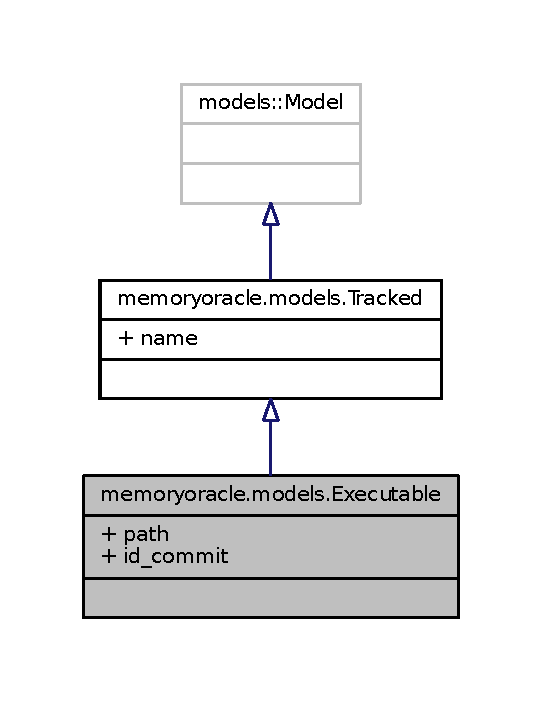
\includegraphics[width=260pt]{classmemoryoracle_1_1models_1_1Executable__inherit__graph}
\end{center}
\end{figure}


Collaboration diagram for memoryoracle.\+models.\+Executable\+:\nopagebreak
\begin{figure}[H]
\begin{center}
\leavevmode
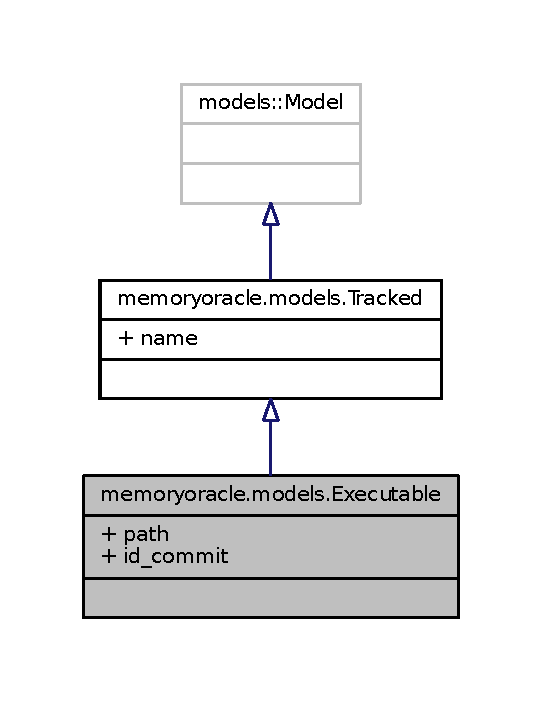
\includegraphics[width=260pt]{classmemoryoracle_1_1models_1_1Executable__coll__graph}
\end{center}
\end{figure}
\subsection*{Classes}
\begin{DoxyCompactItemize}
\item 
class \hyperlink{classmemoryoracle_1_1models_1_1Executable_1_1Meta}{Meta}
\end{DoxyCompactItemize}
\subsection*{Static Public Attributes}
\begin{DoxyCompactItemize}
\item 
tuple \hyperlink{classmemoryoracle_1_1models_1_1Executable_a2ab97065889225c1d050784a374fab8a}{path} = models.\+Text\+Field(default=\char`\"{}./a.\+out\char`\"{})
\item 
tuple \hyperlink{classmemoryoracle_1_1models_1_1Executable_a63ec6fcf966d713361d30913dbeb2815}{id\+\_\+commit} = models.\+Foreign\+Key(\hyperlink{classmemoryoracle_1_1models_1_1Commit}{Commit})
\end{DoxyCompactItemize}


\subsection{Detailed Description}


Definition at line 62 of file models.\+py.



\subsection{Member Data Documentation}
\hypertarget{classmemoryoracle_1_1models_1_1Executable_a63ec6fcf966d713361d30913dbeb2815}{}\index{memoryoracle\+::models\+::\+Executable@{memoryoracle\+::models\+::\+Executable}!id\+\_\+commit@{id\+\_\+commit}}
\index{id\+\_\+commit@{id\+\_\+commit}!memoryoracle\+::models\+::\+Executable@{memoryoracle\+::models\+::\+Executable}}
\subsubsection[{id\+\_\+commit}]{\setlength{\rightskip}{0pt plus 5cm}tuple memoryoracle.\+models.\+Executable.\+id\+\_\+commit = models.\+Foreign\+Key({\bf Commit})\hspace{0.3cm}{\ttfamily [static]}}\label{classmemoryoracle_1_1models_1_1Executable_a63ec6fcf966d713361d30913dbeb2815}


Definition at line 65 of file models.\+py.

\hypertarget{classmemoryoracle_1_1models_1_1Executable_a2ab97065889225c1d050784a374fab8a}{}\index{memoryoracle\+::models\+::\+Executable@{memoryoracle\+::models\+::\+Executable}!path@{path}}
\index{path@{path}!memoryoracle\+::models\+::\+Executable@{memoryoracle\+::models\+::\+Executable}}
\subsubsection[{path}]{\setlength{\rightskip}{0pt plus 5cm}tuple memoryoracle.\+models.\+Executable.\+path = models.\+Text\+Field(default=\char`\"{}./a.\+out\char`\"{})\hspace{0.3cm}{\ttfamily [static]}}\label{classmemoryoracle_1_1models_1_1Executable_a2ab97065889225c1d050784a374fab8a}


Definition at line 64 of file models.\+py.



The documentation for this class was generated from the following file\+:\begin{DoxyCompactItemize}
\item 
memoryoracle/\hyperlink{models_8py}{models.\+py}\end{DoxyCompactItemize}

\hypertarget{classmemoryoracle_1_1test__models_1_1ExecutableTestData}{}\section{memoryoracle.\+test\+\_\+models.\+Executable\+Test\+Data Class Reference}
\label{classmemoryoracle_1_1test__models_1_1ExecutableTestData}\index{memoryoracle.\+test\+\_\+models.\+Executable\+Test\+Data@{memoryoracle.\+test\+\_\+models.\+Executable\+Test\+Data}}


Inheritance diagram for memoryoracle.\+test\+\_\+models.\+Executable\+Test\+Data\+:\nopagebreak
\begin{figure}[H]
\begin{center}
\leavevmode
\includegraphics[width=232pt]{classmemoryoracle_1_1test__models_1_1ExecutableTestData__inherit__graph}
\end{center}
\end{figure}


Collaboration diagram for memoryoracle.\+test\+\_\+models.\+Executable\+Test\+Data\+:\nopagebreak
\begin{figure}[H]
\begin{center}
\leavevmode
\includegraphics[width=232pt]{classmemoryoracle_1_1test__models_1_1ExecutableTestData__coll__graph}
\end{center}
\end{figure}
\subsection*{Public Member Functions}
\begin{DoxyCompactItemize}
\item 
def \hyperlink{classmemoryoracle_1_1test__models_1_1ExecutableTestData_a526f912c2e8eeddb64beb6241f138c09}{set\+\_\+up\+\_\+class} (cls)
\end{DoxyCompactItemize}
\subsection*{Static Public Attributes}
\begin{DoxyCompactItemize}
\item 
\hyperlink{classmemoryoracle_1_1test__models_1_1ExecutableTestData_a81ed1592e6042c61fe80728b55275bdc}{model} = \hyperlink{classmemoryoracle_1_1models_1_1Executable}{memoryoracle.\+models.\+Executable}
\end{DoxyCompactItemize}
\subsection*{Static Private Attributes}
\begin{DoxyCompactItemize}
\item 
list \hyperlink{classmemoryoracle_1_1test__models_1_1ExecutableTestData_a2558978df6fcc2cf6d1a9dadec3ed075}{\+\_\+depends} = \mbox{[}\hyperlink{classmemoryoracle_1_1test__models_1_1CommitTestData}{Commit\+Test\+Data}\mbox{]}
\end{DoxyCompactItemize}
\subsection*{Additional Inherited Members}


\subsection{Detailed Description}


Definition at line 149 of file test\+\_\+models.\+py.



\subsection{Member Function Documentation}
\hypertarget{classmemoryoracle_1_1test__models_1_1ExecutableTestData_a526f912c2e8eeddb64beb6241f138c09}{}\index{memoryoracle\+::test\+\_\+models\+::\+Executable\+Test\+Data@{memoryoracle\+::test\+\_\+models\+::\+Executable\+Test\+Data}!set\+\_\+up\+\_\+class@{set\+\_\+up\+\_\+class}}
\index{set\+\_\+up\+\_\+class@{set\+\_\+up\+\_\+class}!memoryoracle\+::test\+\_\+models\+::\+Executable\+Test\+Data@{memoryoracle\+::test\+\_\+models\+::\+Executable\+Test\+Data}}
\subsubsection[{set\+\_\+up\+\_\+class}]{\setlength{\rightskip}{0pt plus 5cm}def memoryoracle.\+test\+\_\+models.\+Executable\+Test\+Data.\+set\+\_\+up\+\_\+class (
\begin{DoxyParamCaption}
\item[{}]{cls}
\end{DoxyParamCaption}
)}\label{classmemoryoracle_1_1test__models_1_1ExecutableTestData_a526f912c2e8eeddb64beb6241f138c09}


Definition at line 156 of file test\+\_\+models.\+py.



References memoryoracle.\+instance.\+x.


\begin{DoxyCode}
156     \textcolor{keyword}{def }\hyperlink{classmemoryoracle_1_1test__models_1_1ExecutableTestData_a526f912c2e8eeddb64beb6241f138c09}{set\_up\_class}(cls):
157         cls.set\_up\_depends()
158         cls.data = \{ x.\_\_name\_\_: \hyperlink{namespacememoryoracle_1_1instance_afe036cc8dc71469743d090c4c80d50c5}{x}() \textcolor{keywordflow}{for} x \textcolor{keywordflow}{in} cls.depends() \}
159         cls.argsList = [
160                 \{
161                     \textcolor{stringliteral}{"name"}: ModelTestData.gen\_name(),
162                     \textcolor{stringliteral}{"path"}: ModelTestData.gen\_name(),
163                     \textcolor{stringliteral}{"id\_commit"}: commit,
164                 \} \textcolor{keywordflow}{for} commit \textcolor{keywordflow}{in} cls.data[\textcolor{stringliteral}{"CommitTestData"}] ]
165         cls.orms = [ cls.model.objects.create(**kwargs) \textcolor{keywordflow}{for} kwargs \textcolor{keywordflow}{in} cls.argsList ]
166 
167 
\end{DoxyCode}


\subsection{Member Data Documentation}
\hypertarget{classmemoryoracle_1_1test__models_1_1ExecutableTestData_a2558978df6fcc2cf6d1a9dadec3ed075}{}\index{memoryoracle\+::test\+\_\+models\+::\+Executable\+Test\+Data@{memoryoracle\+::test\+\_\+models\+::\+Executable\+Test\+Data}!\+\_\+depends@{\+\_\+depends}}
\index{\+\_\+depends@{\+\_\+depends}!memoryoracle\+::test\+\_\+models\+::\+Executable\+Test\+Data@{memoryoracle\+::test\+\_\+models\+::\+Executable\+Test\+Data}}
\subsubsection[{\+\_\+depends}]{\setlength{\rightskip}{0pt plus 5cm}list memoryoracle.\+test\+\_\+models.\+Executable\+Test\+Data.\+\_\+depends = \mbox{[}{\bf Commit\+Test\+Data}\mbox{]}\hspace{0.3cm}{\ttfamily [static]}, {\ttfamily [private]}}\label{classmemoryoracle_1_1test__models_1_1ExecutableTestData_a2558978df6fcc2cf6d1a9dadec3ed075}


Definition at line 153 of file test\+\_\+models.\+py.

\hypertarget{classmemoryoracle_1_1test__models_1_1ExecutableTestData_a81ed1592e6042c61fe80728b55275bdc}{}\index{memoryoracle\+::test\+\_\+models\+::\+Executable\+Test\+Data@{memoryoracle\+::test\+\_\+models\+::\+Executable\+Test\+Data}!model@{model}}
\index{model@{model}!memoryoracle\+::test\+\_\+models\+::\+Executable\+Test\+Data@{memoryoracle\+::test\+\_\+models\+::\+Executable\+Test\+Data}}
\subsubsection[{model}]{\setlength{\rightskip}{0pt plus 5cm}memoryoracle.\+test\+\_\+models.\+Executable\+Test\+Data.\+model = {\bf memoryoracle.\+models.\+Executable}\hspace{0.3cm}{\ttfamily [static]}}\label{classmemoryoracle_1_1test__models_1_1ExecutableTestData_a81ed1592e6042c61fe80728b55275bdc}


Definition at line 151 of file test\+\_\+models.\+py.



The documentation for this class was generated from the following file\+:\begin{DoxyCompactItemize}
\item 
memoryoracle/\hyperlink{test__models_8py}{test\+\_\+models.\+py}\end{DoxyCompactItemize}

\hypertarget{classmemoryoracle_1_1models_1_1Execution}{}\section{memoryoracle.\+models.\+Execution Class Reference}
\label{classmemoryoracle_1_1models_1_1Execution}\index{memoryoracle.\+models.\+Execution@{memoryoracle.\+models.\+Execution}}


Inheritance diagram for memoryoracle.\+models.\+Execution\+:\nopagebreak
\begin{figure}[H]
\begin{center}
\leavevmode
\includegraphics[width=254pt]{classmemoryoracle_1_1models_1_1Execution__inherit__graph}
\end{center}
\end{figure}


Collaboration diagram for memoryoracle.\+models.\+Execution\+:\nopagebreak
\begin{figure}[H]
\begin{center}
\leavevmode
\includegraphics[width=254pt]{classmemoryoracle_1_1models_1_1Execution__coll__graph}
\end{center}
\end{figure}
\subsection*{Classes}
\begin{DoxyCompactItemize}
\item 
class \hyperlink{classmemoryoracle_1_1models_1_1Execution_1_1Meta}{Meta}
\end{DoxyCompactItemize}
\subsection*{Static Public Attributes}
\begin{DoxyCompactItemize}
\item 
tuple \hyperlink{classmemoryoracle_1_1models_1_1Execution_a126d2c8175a946f7b6b1276f4a58e432}{id\+\_\+executable} = models.\+Foreign\+Key(\hyperlink{classmemoryoracle_1_1models_1_1Executable}{Executable}, default=None)
\end{DoxyCompactItemize}


\subsection{Detailed Description}


Definition at line 71 of file models.\+py.



\subsection{Member Data Documentation}
\hypertarget{classmemoryoracle_1_1models_1_1Execution_a126d2c8175a946f7b6b1276f4a58e432}{}\index{memoryoracle\+::models\+::\+Execution@{memoryoracle\+::models\+::\+Execution}!id\+\_\+executable@{id\+\_\+executable}}
\index{id\+\_\+executable@{id\+\_\+executable}!memoryoracle\+::models\+::\+Execution@{memoryoracle\+::models\+::\+Execution}}
\subsubsection[{id\+\_\+executable}]{\setlength{\rightskip}{0pt plus 5cm}tuple memoryoracle.\+models.\+Execution.\+id\+\_\+executable = models.\+Foreign\+Key({\bf Executable}, default=None)\hspace{0.3cm}{\ttfamily [static]}}\label{classmemoryoracle_1_1models_1_1Execution_a126d2c8175a946f7b6b1276f4a58e432}


Definition at line 73 of file models.\+py.



The documentation for this class was generated from the following file\+:\begin{DoxyCompactItemize}
\item 
memoryoracle/\hyperlink{models_8py}{models.\+py}\end{DoxyCompactItemize}

\hypertarget{classmemoryoracle_1_1execution_1_1Execution}{}\section{memoryoracle.\+execution.\+Execution Class Reference}
\label{classmemoryoracle_1_1execution_1_1Execution}\index{memoryoracle.\+execution.\+Execution@{memoryoracle.\+execution.\+Execution}}


Inheritance diagram for memoryoracle.\+execution.\+Execution\+:
\nopagebreak
\begin{figure}[H]
\begin{center}
\leavevmode
\includegraphics[width=265pt]{classmemoryoracle_1_1execution_1_1Execution__inherit__graph}
\end{center}
\end{figure}


Collaboration diagram for memoryoracle.\+execution.\+Execution\+:
\nopagebreak
\begin{figure}[H]
\begin{center}
\leavevmode
\includegraphics[width=265pt]{classmemoryoracle_1_1execution_1_1Execution__coll__graph}
\end{center}
\end{figure}
\subsection*{Static Public Attributes}
\begin{DoxyCompactItemize}
\item 
tuple \hyperlink{classmemoryoracle_1_1execution_1_1Execution_a663a215430b1923fdbdc15e4a081c241}{arguments} = mongoengine.\+String\+Field()
\item 
tuple \hyperlink{classmemoryoracle_1_1execution_1_1Execution_abe961abfe6caa800e16358a58572eff3}{start\+\_\+time} = mongoengine.\+Complex\+Date\+Time\+Field()
\item 
tuple \hyperlink{classmemoryoracle_1_1execution_1_1Execution_ac03f8d74970a2dcf7e84bf109052118c}{end\+\_\+time} = mongoengine.\+Complex\+Date\+Time\+Field()
\item 
tuple \hyperlink{classmemoryoracle_1_1execution_1_1Execution_a3aeb1a80427e0101619b2db1c43e7e0c}{objects} = mongoengine.\+List\+Field(mongoengine.\+Reference\+Field(\hyperlink{classmemoryoracle_1_1execution_1_1Instance}{Instance}))
\end{DoxyCompactItemize}


\subsection{Detailed Description}
\begin{DoxyVerb}*Concrete* class representing a particular call to an executable.
\end{DoxyVerb}
 

Definition at line 24 of file execution.\+py.



\subsection{Member Data Documentation}
\hypertarget{classmemoryoracle_1_1execution_1_1Execution_a663a215430b1923fdbdc15e4a081c241}{}\index{memoryoracle\+::execution\+::\+Execution@{memoryoracle\+::execution\+::\+Execution}!arguments@{arguments}}
\index{arguments@{arguments}!memoryoracle\+::execution\+::\+Execution@{memoryoracle\+::execution\+::\+Execution}}
\subsubsection[{arguments}]{\setlength{\rightskip}{0pt plus 5cm}tuple memoryoracle.\+execution.\+Execution.\+arguments = mongoengine.\+String\+Field()\hspace{0.3cm}{\ttfamily [static]}}\label{classmemoryoracle_1_1execution_1_1Execution_a663a215430b1923fdbdc15e4a081c241}


Definition at line 28 of file execution.\+py.

\hypertarget{classmemoryoracle_1_1execution_1_1Execution_ac03f8d74970a2dcf7e84bf109052118c}{}\index{memoryoracle\+::execution\+::\+Execution@{memoryoracle\+::execution\+::\+Execution}!end\+\_\+time@{end\+\_\+time}}
\index{end\+\_\+time@{end\+\_\+time}!memoryoracle\+::execution\+::\+Execution@{memoryoracle\+::execution\+::\+Execution}}
\subsubsection[{end\+\_\+time}]{\setlength{\rightskip}{0pt plus 5cm}tuple memoryoracle.\+execution.\+Execution.\+end\+\_\+time = mongoengine.\+Complex\+Date\+Time\+Field()\hspace{0.3cm}{\ttfamily [static]}}\label{classmemoryoracle_1_1execution_1_1Execution_ac03f8d74970a2dcf7e84bf109052118c}


Definition at line 30 of file execution.\+py.

\hypertarget{classmemoryoracle_1_1execution_1_1Execution_a3aeb1a80427e0101619b2db1c43e7e0c}{}\index{memoryoracle\+::execution\+::\+Execution@{memoryoracle\+::execution\+::\+Execution}!objects@{objects}}
\index{objects@{objects}!memoryoracle\+::execution\+::\+Execution@{memoryoracle\+::execution\+::\+Execution}}
\subsubsection[{objects}]{\setlength{\rightskip}{0pt plus 5cm}tuple memoryoracle.\+execution.\+Execution.\+objects = mongoengine.\+List\+Field(mongoengine.\+Reference\+Field({\bf Instance}))\hspace{0.3cm}{\ttfamily [static]}}\label{classmemoryoracle_1_1execution_1_1Execution_a3aeb1a80427e0101619b2db1c43e7e0c}


Definition at line 32 of file execution.\+py.

\hypertarget{classmemoryoracle_1_1execution_1_1Execution_abe961abfe6caa800e16358a58572eff3}{}\index{memoryoracle\+::execution\+::\+Execution@{memoryoracle\+::execution\+::\+Execution}!start\+\_\+time@{start\+\_\+time}}
\index{start\+\_\+time@{start\+\_\+time}!memoryoracle\+::execution\+::\+Execution@{memoryoracle\+::execution\+::\+Execution}}
\subsubsection[{start\+\_\+time}]{\setlength{\rightskip}{0pt plus 5cm}tuple memoryoracle.\+execution.\+Execution.\+start\+\_\+time = mongoengine.\+Complex\+Date\+Time\+Field()\hspace{0.3cm}{\ttfamily [static]}}\label{classmemoryoracle_1_1execution_1_1Execution_abe961abfe6caa800e16358a58572eff3}


Definition at line 29 of file execution.\+py.



The documentation for this class was generated from the following file\+:\begin{DoxyCompactItemize}
\item 
memoryoracle/\hyperlink{execution_8py}{execution.\+py}\end{DoxyCompactItemize}

\hypertarget{classmemoryoracle_1_1test__models_1_1ExecutionTestData}{}\section{memoryoracle.\+test\+\_\+models.\+Execution\+Test\+Data Class Reference}
\label{classmemoryoracle_1_1test__models_1_1ExecutionTestData}\index{memoryoracle.\+test\+\_\+models.\+Execution\+Test\+Data@{memoryoracle.\+test\+\_\+models.\+Execution\+Test\+Data}}


Inheritance diagram for memoryoracle.\+test\+\_\+models.\+Execution\+Test\+Data\+:\nopagebreak
\begin{figure}[H]
\begin{center}
\leavevmode
\includegraphics[width=232pt]{classmemoryoracle_1_1test__models_1_1ExecutionTestData__inherit__graph}
\end{center}
\end{figure}


Collaboration diagram for memoryoracle.\+test\+\_\+models.\+Execution\+Test\+Data\+:\nopagebreak
\begin{figure}[H]
\begin{center}
\leavevmode
\includegraphics[width=232pt]{classmemoryoracle_1_1test__models_1_1ExecutionTestData__coll__graph}
\end{center}
\end{figure}
\subsection*{Public Member Functions}
\begin{DoxyCompactItemize}
\item 
def \hyperlink{classmemoryoracle_1_1test__models_1_1ExecutionTestData_aee8f3379c92809ba79acff8c1cac48c9}{set\+\_\+up\+\_\+class} (cls)
\end{DoxyCompactItemize}
\subsection*{Static Public Attributes}
\begin{DoxyCompactItemize}
\item 
\hyperlink{classmemoryoracle_1_1test__models_1_1ExecutionTestData_a6e5285d5b3b3ff2443ec195959d31213}{model} = \hyperlink{classmemoryoracle_1_1models_1_1Execution}{memoryoracle.\+models.\+Execution}
\end{DoxyCompactItemize}
\subsection*{Static Private Attributes}
\begin{DoxyCompactItemize}
\item 
list \hyperlink{classmemoryoracle_1_1test__models_1_1ExecutionTestData_a2755e7fbb9b8274fd4572c36bb37e27c}{\+\_\+depends} = \mbox{[}\hyperlink{classmemoryoracle_1_1test__models_1_1ExecutableTestData}{Executable\+Test\+Data}\mbox{]}
\end{DoxyCompactItemize}
\subsection*{Additional Inherited Members}


\subsection{Detailed Description}


Definition at line 183 of file test\+\_\+models.\+py.



\subsection{Member Function Documentation}
\hypertarget{classmemoryoracle_1_1test__models_1_1ExecutionTestData_aee8f3379c92809ba79acff8c1cac48c9}{}\index{memoryoracle\+::test\+\_\+models\+::\+Execution\+Test\+Data@{memoryoracle\+::test\+\_\+models\+::\+Execution\+Test\+Data}!set\+\_\+up\+\_\+class@{set\+\_\+up\+\_\+class}}
\index{set\+\_\+up\+\_\+class@{set\+\_\+up\+\_\+class}!memoryoracle\+::test\+\_\+models\+::\+Execution\+Test\+Data@{memoryoracle\+::test\+\_\+models\+::\+Execution\+Test\+Data}}
\subsubsection[{set\+\_\+up\+\_\+class}]{\setlength{\rightskip}{0pt plus 5cm}def memoryoracle.\+test\+\_\+models.\+Execution\+Test\+Data.\+set\+\_\+up\+\_\+class (
\begin{DoxyParamCaption}
\item[{}]{cls}
\end{DoxyParamCaption}
)}\label{classmemoryoracle_1_1test__models_1_1ExecutionTestData_aee8f3379c92809ba79acff8c1cac48c9}


Definition at line 190 of file test\+\_\+models.\+py.



References memoryoracle.\+instance.\+x.


\begin{DoxyCode}
190     \textcolor{keyword}{def }\hyperlink{classmemoryoracle_1_1test__models_1_1ExecutionTestData_aee8f3379c92809ba79acff8c1cac48c9}{set\_up\_class}(cls):
191         cls.set\_up\_depends()
192         cls.data = \{ x.\_\_name\_\_: \hyperlink{namespacememoryoracle_1_1instance_afe036cc8dc71469743d090c4c80d50c5}{x}() \textcolor{keywordflow}{for} x \textcolor{keywordflow}{in} cls.depends() \}
193         cls.argsList = [
194                 \{
195                     \textcolor{stringliteral}{"name"}: ModelTestData.gen\_name(),
196                     \textcolor{stringliteral}{"id\_executable"}: executable,
197                 \} \textcolor{keywordflow}{for} executable \textcolor{keywordflow}{in} cls.data[\textcolor{stringliteral}{"ExecutableTestData"}] ]
198         cls.orms = [ cls.model.objects.create(**kwargs) \textcolor{keywordflow}{for} kwargs \textcolor{keywordflow}{in} cls.argsList ]
199 
200 
\end{DoxyCode}


\subsection{Member Data Documentation}
\hypertarget{classmemoryoracle_1_1test__models_1_1ExecutionTestData_a2755e7fbb9b8274fd4572c36bb37e27c}{}\index{memoryoracle\+::test\+\_\+models\+::\+Execution\+Test\+Data@{memoryoracle\+::test\+\_\+models\+::\+Execution\+Test\+Data}!\+\_\+depends@{\+\_\+depends}}
\index{\+\_\+depends@{\+\_\+depends}!memoryoracle\+::test\+\_\+models\+::\+Execution\+Test\+Data@{memoryoracle\+::test\+\_\+models\+::\+Execution\+Test\+Data}}
\subsubsection[{\+\_\+depends}]{\setlength{\rightskip}{0pt plus 5cm}list memoryoracle.\+test\+\_\+models.\+Execution\+Test\+Data.\+\_\+depends = \mbox{[}{\bf Executable\+Test\+Data}\mbox{]}\hspace{0.3cm}{\ttfamily [static]}, {\ttfamily [private]}}\label{classmemoryoracle_1_1test__models_1_1ExecutionTestData_a2755e7fbb9b8274fd4572c36bb37e27c}


Definition at line 187 of file test\+\_\+models.\+py.

\hypertarget{classmemoryoracle_1_1test__models_1_1ExecutionTestData_a6e5285d5b3b3ff2443ec195959d31213}{}\index{memoryoracle\+::test\+\_\+models\+::\+Execution\+Test\+Data@{memoryoracle\+::test\+\_\+models\+::\+Execution\+Test\+Data}!model@{model}}
\index{model@{model}!memoryoracle\+::test\+\_\+models\+::\+Execution\+Test\+Data@{memoryoracle\+::test\+\_\+models\+::\+Execution\+Test\+Data}}
\subsubsection[{model}]{\setlength{\rightskip}{0pt plus 5cm}memoryoracle.\+test\+\_\+models.\+Execution\+Test\+Data.\+model = {\bf memoryoracle.\+models.\+Execution}\hspace{0.3cm}{\ttfamily [static]}}\label{classmemoryoracle_1_1test__models_1_1ExecutionTestData_a6e5285d5b3b3ff2443ec195959d31213}


Definition at line 185 of file test\+\_\+models.\+py.



The documentation for this class was generated from the following file\+:\begin{DoxyCompactItemize}
\item 
memoryoracle/\hyperlink{test__models_8py}{test\+\_\+models.\+py}\end{DoxyCompactItemize}

\hypertarget{classmemoryoracle_1_1descriptions_1_1ExternalDescriptionDecorator}{}\section{memoryoracle.\+descriptions.\+External\+Description\+Decorator Class Reference}
\label{classmemoryoracle_1_1descriptions_1_1ExternalDescriptionDecorator}\index{memoryoracle.\+descriptions.\+External\+Description\+Decorator@{memoryoracle.\+descriptions.\+External\+Description\+Decorator}}


Inheritance diagram for memoryoracle.\+descriptions.\+External\+Description\+Decorator\+:\nopagebreak
\begin{figure}[H]
\begin{center}
\leavevmode
\includegraphics[width=238pt]{classmemoryoracle_1_1descriptions_1_1ExternalDescriptionDecorator__inherit__graph}
\end{center}
\end{figure}


Collaboration diagram for memoryoracle.\+descriptions.\+External\+Description\+Decorator\+:\nopagebreak
\begin{figure}[H]
\begin{center}
\leavevmode
\includegraphics[width=238pt]{classmemoryoracle_1_1descriptions_1_1ExternalDescriptionDecorator__coll__graph}
\end{center}
\end{figure}
\subsection*{Public Member Functions}
\begin{DoxyCompactItemize}
\item 
def \hyperlink{classmemoryoracle_1_1descriptions_1_1ExternalDescriptionDecorator_afeb1f6dd877cc71d89def903ffd781d6}{\+\_\+\+\_\+init\+\_\+\+\_\+} (self, \hyperlink{classmemoryoracle_1_1descriptions_1_1ExternalDescriptionDecorator_ae5952e51de2c9473ce19875b55ccb625}{description})
\item 
def \hyperlink{classmemoryoracle_1_1descriptions_1_1ExternalDescriptionDecorator_ae5952e51de2c9473ce19875b55ccb625}{description} (self)
\item 
def \hyperlink{classmemoryoracle_1_1descriptions_1_1ExternalDescriptionDecorator_a3653b421084fc367f59e1b365270d4e1}{name} (self)
\end{DoxyCompactItemize}
\subsection*{Private Attributes}
\begin{DoxyCompactItemize}
\item 
\hyperlink{classmemoryoracle_1_1descriptions_1_1ExternalDescriptionDecorator_ae42579816acbf90c9a28395fa0d55786}{\+\_\+description}
\end{DoxyCompactItemize}


\subsection{Detailed Description}
\begin{DoxyVerb}*Decorator* ExternalDescriptionDecorator class.

A decorator to mark another description as refering to an
external piece of information, such as a standard library
header file or a library file which is external to your
project.
\end{DoxyVerb}
 

Definition at line 62 of file descriptions.\+py.



\subsection{Constructor \& Destructor Documentation}
\hypertarget{classmemoryoracle_1_1descriptions_1_1ExternalDescriptionDecorator_afeb1f6dd877cc71d89def903ffd781d6}{}\index{memoryoracle\+::descriptions\+::\+External\+Description\+Decorator@{memoryoracle\+::descriptions\+::\+External\+Description\+Decorator}!\+\_\+\+\_\+init\+\_\+\+\_\+@{\+\_\+\+\_\+init\+\_\+\+\_\+}}
\index{\+\_\+\+\_\+init\+\_\+\+\_\+@{\+\_\+\+\_\+init\+\_\+\+\_\+}!memoryoracle\+::descriptions\+::\+External\+Description\+Decorator@{memoryoracle\+::descriptions\+::\+External\+Description\+Decorator}}
\subsubsection[{\+\_\+\+\_\+init\+\_\+\+\_\+}]{\setlength{\rightskip}{0pt plus 5cm}def memoryoracle.\+descriptions.\+External\+Description\+Decorator.\+\_\+\+\_\+init\+\_\+\+\_\+ (
\begin{DoxyParamCaption}
\item[{}]{self, }
\item[{}]{description}
\end{DoxyParamCaption}
)}\label{classmemoryoracle_1_1descriptions_1_1ExternalDescriptionDecorator_afeb1f6dd877cc71d89def903ffd781d6}


Definition at line 72 of file descriptions.\+py.


\begin{DoxyCode}
72     \textcolor{keyword}{def }\hyperlink{classmemoryoracle_1_1descriptions_1_1ExternalDescriptionDecorator_afeb1f6dd877cc71d89def903ffd781d6}{\_\_init\_\_}(self, description):
73         self.\hyperlink{classmemoryoracle_1_1descriptions_1_1ExternalDescriptionDecorator_ae42579816acbf90c9a28395fa0d55786}{\_description} = description
74 
\end{DoxyCode}


\subsection{Member Function Documentation}
\hypertarget{classmemoryoracle_1_1descriptions_1_1ExternalDescriptionDecorator_ae5952e51de2c9473ce19875b55ccb625}{}\index{memoryoracle\+::descriptions\+::\+External\+Description\+Decorator@{memoryoracle\+::descriptions\+::\+External\+Description\+Decorator}!description@{description}}
\index{description@{description}!memoryoracle\+::descriptions\+::\+External\+Description\+Decorator@{memoryoracle\+::descriptions\+::\+External\+Description\+Decorator}}
\subsubsection[{description}]{\setlength{\rightskip}{0pt plus 5cm}def memoryoracle.\+descriptions.\+External\+Description\+Decorator.\+description (
\begin{DoxyParamCaption}
\item[{}]{self}
\end{DoxyParamCaption}
)}\label{classmemoryoracle_1_1descriptions_1_1ExternalDescriptionDecorator_ae5952e51de2c9473ce19875b55ccb625}


Definition at line 76 of file descriptions.\+py.



References memoryoracle.\+descriptions.\+Black\+Box\+Decorator.\+\_\+description, and memoryoracle.\+descriptions.\+External\+Description\+Decorator.\+\_\+description.



Referenced by memoryoracle.\+instance.\+Int.\+\_\+track().


\begin{DoxyCode}
76     \textcolor{keyword}{def }\hyperlink{classmemoryoracle_1_1descriptions_1_1ExternalDescriptionDecorator_ae5952e51de2c9473ce19875b55ccb625}{description}(self):
77         \textcolor{keywordflow}{return} \{ \textcolor{stringliteral}{"external"}: self.\hyperlink{classmemoryoracle_1_1descriptions_1_1ExternalDescriptionDecorator_ae42579816acbf90c9a28395fa0d55786}{\_description} \}
78 
\end{DoxyCode}


Here is the caller graph for this function\+:
\nopagebreak
\begin{figure}[H]
\begin{center}
\leavevmode
\includegraphics[width=350pt]{classmemoryoracle_1_1descriptions_1_1ExternalDescriptionDecorator_ae5952e51de2c9473ce19875b55ccb625_icgraph}
\end{center}
\end{figure}


\hypertarget{classmemoryoracle_1_1descriptions_1_1ExternalDescriptionDecorator_a3653b421084fc367f59e1b365270d4e1}{}\index{memoryoracle\+::descriptions\+::\+External\+Description\+Decorator@{memoryoracle\+::descriptions\+::\+External\+Description\+Decorator}!name@{name}}
\index{name@{name}!memoryoracle\+::descriptions\+::\+External\+Description\+Decorator@{memoryoracle\+::descriptions\+::\+External\+Description\+Decorator}}
\subsubsection[{name}]{\setlength{\rightskip}{0pt plus 5cm}def memoryoracle.\+descriptions.\+External\+Description\+Decorator.\+name (
\begin{DoxyParamCaption}
\item[{}]{self}
\end{DoxyParamCaption}
)}\label{classmemoryoracle_1_1descriptions_1_1ExternalDescriptionDecorator_a3653b421084fc367f59e1b365270d4e1}


Definition at line 80 of file descriptions.\+py.


\begin{DoxyCode}
80     \textcolor{keyword}{def }\hyperlink{classmemoryoracle_1_1descriptions_1_1ExternalDescriptionDecorator_a3653b421084fc367f59e1b365270d4e1}{name}(self):
81         \textcolor{keywordflow}{return} self.\_description.name
82 
83 
\end{DoxyCode}


\subsection{Member Data Documentation}
\hypertarget{classmemoryoracle_1_1descriptions_1_1ExternalDescriptionDecorator_ae42579816acbf90c9a28395fa0d55786}{}\index{memoryoracle\+::descriptions\+::\+External\+Description\+Decorator@{memoryoracle\+::descriptions\+::\+External\+Description\+Decorator}!\+\_\+description@{\+\_\+description}}
\index{\+\_\+description@{\+\_\+description}!memoryoracle\+::descriptions\+::\+External\+Description\+Decorator@{memoryoracle\+::descriptions\+::\+External\+Description\+Decorator}}
\subsubsection[{\+\_\+description}]{\setlength{\rightskip}{0pt plus 5cm}memoryoracle.\+descriptions.\+External\+Description\+Decorator.\+\_\+description\hspace{0.3cm}{\ttfamily [private]}}\label{classmemoryoracle_1_1descriptions_1_1ExternalDescriptionDecorator_ae42579816acbf90c9a28395fa0d55786}


Definition at line 73 of file descriptions.\+py.



Referenced by memoryoracle.\+tracked.\+Tracked.\+description(), memoryoracle.\+descriptions.\+External\+Description\+Decorator.\+description(), and memoryoracle.\+descriptions.\+Standard\+Description\+Decorator.\+description().



The documentation for this class was generated from the following file\+:\begin{DoxyCompactItemize}
\item 
memoryoracle/\hyperlink{descriptions_8py}{descriptions.\+py}\end{DoxyCompactItemize}

\hypertarget{classmemoryoracle_1_1instance_1_1ExternDecorator}{}\section{memoryoracle.\+instance.\+Extern\+Decorator Class Reference}
\label{classmemoryoracle_1_1instance_1_1ExternDecorator}\index{memoryoracle.\+instance.\+Extern\+Decorator@{memoryoracle.\+instance.\+Extern\+Decorator}}


Inheritance diagram for memoryoracle.\+instance.\+Extern\+Decorator\+:
\nopagebreak
\begin{figure}[H]
\begin{center}
\leavevmode
\includegraphics[height=550pt]{classmemoryoracle_1_1instance_1_1ExternDecorator__inherit__graph}
\end{center}
\end{figure}


Collaboration diagram for memoryoracle.\+instance.\+Extern\+Decorator\+:
\nopagebreak
\begin{figure}[H]
\begin{center}
\leavevmode
\includegraphics[height=550pt]{classmemoryoracle_1_1instance_1_1ExternDecorator__coll__graph}
\end{center}
\end{figure}
\subsection*{Additional Inherited Members}


\subsection{Detailed Description}
\begin{DoxyVerb}*Decorator* class to decorate an addressable as being marked extern.
\end{DoxyVerb}
 

Definition at line 248 of file instance.\+py.



The documentation for this class was generated from the following file\+:\begin{DoxyCompactItemize}
\item 
memoryoracle/\hyperlink{instance_8py}{instance.\+py}\end{DoxyCompactItemize}

\hypertarget{classmemoryoracle_1_1descriptions_1_1FileDescription}{}\section{memoryoracle.\+descriptions.\+File\+Description Class Reference}
\label{classmemoryoracle_1_1descriptions_1_1FileDescription}\index{memoryoracle.\+descriptions.\+File\+Description@{memoryoracle.\+descriptions.\+File\+Description}}


Inheritance diagram for memoryoracle.\+descriptions.\+File\+Description\+:\nopagebreak
\begin{figure}[H]
\begin{center}
\leavevmode
\includegraphics[width=350pt]{classmemoryoracle_1_1descriptions_1_1FileDescription__inherit__graph}
\end{center}
\end{figure}


Collaboration diagram for memoryoracle.\+descriptions.\+File\+Description\+:\nopagebreak
\begin{figure}[H]
\begin{center}
\leavevmode
\includegraphics[width=230pt]{classmemoryoracle_1_1descriptions_1_1FileDescription__coll__graph}
\end{center}
\end{figure}
\subsection*{Additional Inherited Members}


\subsection{Detailed Description}
\begin{DoxyVerb}*Abstract* FileDescription class.

A description of a file object.
\end{DoxyVerb}
 

Definition at line 104 of file descriptions.\+py.



The documentation for this class was generated from the following file\+:\begin{DoxyCompactItemize}
\item 
memoryoracle/\hyperlink{descriptions_8py}{descriptions.\+py}\end{DoxyCompactItemize}

\hypertarget{classmemoryoracle_1_1instance_1_1Float}{}\section{memoryoracle.\+instance.\+Float Class Reference}
\label{classmemoryoracle_1_1instance_1_1Float}\index{memoryoracle.\+instance.\+Float@{memoryoracle.\+instance.\+Float}}


Inheritance diagram for memoryoracle.\+instance.\+Float\+:
\nopagebreak
\begin{figure}[H]
\begin{center}
\leavevmode
\includegraphics[height=550pt]{classmemoryoracle_1_1instance_1_1Float__inherit__graph}
\end{center}
\end{figure}


Collaboration diagram for memoryoracle.\+instance.\+Float\+:
\nopagebreak
\begin{figure}[H]
\begin{center}
\leavevmode
\includegraphics[height=550pt]{classmemoryoracle_1_1instance_1_1Float__coll__graph}
\end{center}
\end{figure}
\subsection*{Static Public Attributes}
\begin{DoxyCompactItemize}
\item 
tuple \hyperlink{classmemoryoracle_1_1instance_1_1Float_a95b3997824e3c9223128f07ef7c69a19}{repository} = dict()
\end{DoxyCompactItemize}
\subsection*{Static Private Attributes}
\begin{DoxyCompactItemize}
\item 
tuple \hyperlink{classmemoryoracle_1_1instance_1_1Float_a2de362a0f4b3b80cfcb0ad7d09cd1462}{\+\_\+update\+Tracker} = set()
\item 
tuple \hyperlink{classmemoryoracle_1_1instance_1_1Float_a41aab3bf3c399c2a8762081fc3b326ee}{\+\_\+watchers} = dict()
\item 
\hyperlink{classmemoryoracle_1_1instance_1_1Float_ac8210ee0f50a53fff0d84f4a80335250}{\+\_\+type\+Handler\+Code} = gdb.\+T\+Y\+P\+E\+\_\+\+C\+O\+D\+E\+\_\+\+F\+L\+T
\end{DoxyCompactItemize}
\subsection*{Additional Inherited Members}


\subsection{Detailed Description}
\begin{DoxyVerb}*Concrete* class to represent floating point primitivies.
\end{DoxyVerb}
 

Definition at line 445 of file instance.\+py.



\subsection{Member Data Documentation}
\hypertarget{classmemoryoracle_1_1instance_1_1Float_ac8210ee0f50a53fff0d84f4a80335250}{}\index{memoryoracle\+::instance\+::\+Float@{memoryoracle\+::instance\+::\+Float}!\+\_\+type\+Handler\+Code@{\+\_\+type\+Handler\+Code}}
\index{\+\_\+type\+Handler\+Code@{\+\_\+type\+Handler\+Code}!memoryoracle\+::instance\+::\+Float@{memoryoracle\+::instance\+::\+Float}}
\subsubsection[{\+\_\+type\+Handler\+Code}]{\setlength{\rightskip}{0pt plus 5cm}memoryoracle.\+instance.\+Float.\+\_\+type\+Handler\+Code = gdb.\+T\+Y\+P\+E\+\_\+\+C\+O\+D\+E\+\_\+\+F\+L\+T\hspace{0.3cm}{\ttfamily [static]}, {\ttfamily [private]}}\label{classmemoryoracle_1_1instance_1_1Float_ac8210ee0f50a53fff0d84f4a80335250}


Definition at line 453 of file instance.\+py.



Referenced by memoryoracle.\+models.\+Typed.\+type\+\_\+handler().

\hypertarget{classmemoryoracle_1_1instance_1_1Float_a2de362a0f4b3b80cfcb0ad7d09cd1462}{}\index{memoryoracle\+::instance\+::\+Float@{memoryoracle\+::instance\+::\+Float}!\+\_\+update\+Tracker@{\+\_\+update\+Tracker}}
\index{\+\_\+update\+Tracker@{\+\_\+update\+Tracker}!memoryoracle\+::instance\+::\+Float@{memoryoracle\+::instance\+::\+Float}}
\subsubsection[{\+\_\+update\+Tracker}]{\setlength{\rightskip}{0pt plus 5cm}tuple memoryoracle.\+instance.\+Float.\+\_\+update\+Tracker = set()\hspace{0.3cm}{\ttfamily [static]}, {\ttfamily [private]}}\label{classmemoryoracle_1_1instance_1_1Float_a2de362a0f4b3b80cfcb0ad7d09cd1462}


Definition at line 450 of file instance.\+py.

\hypertarget{classmemoryoracle_1_1instance_1_1Float_a41aab3bf3c399c2a8762081fc3b326ee}{}\index{memoryoracle\+::instance\+::\+Float@{memoryoracle\+::instance\+::\+Float}!\+\_\+watchers@{\+\_\+watchers}}
\index{\+\_\+watchers@{\+\_\+watchers}!memoryoracle\+::instance\+::\+Float@{memoryoracle\+::instance\+::\+Float}}
\subsubsection[{\+\_\+watchers}]{\setlength{\rightskip}{0pt plus 5cm}tuple memoryoracle.\+instance.\+Float.\+\_\+watchers = dict()\hspace{0.3cm}{\ttfamily [static]}, {\ttfamily [private]}}\label{classmemoryoracle_1_1instance_1_1Float_a41aab3bf3c399c2a8762081fc3b326ee}


Definition at line 451 of file instance.\+py.



Referenced by memoryoracle.\+models.\+Typed.\+\_\+\+\_\+init\+\_\+\+\_\+(), and memoryoracle.\+models.\+Memory.\+watchers().

\hypertarget{classmemoryoracle_1_1instance_1_1Float_a95b3997824e3c9223128f07ef7c69a19}{}\index{memoryoracle\+::instance\+::\+Float@{memoryoracle\+::instance\+::\+Float}!repository@{repository}}
\index{repository@{repository}!memoryoracle\+::instance\+::\+Float@{memoryoracle\+::instance\+::\+Float}}
\subsubsection[{repository}]{\setlength{\rightskip}{0pt plus 5cm}tuple memoryoracle.\+instance.\+Float.\+repository = dict()\hspace{0.3cm}{\ttfamily [static]}}\label{classmemoryoracle_1_1instance_1_1Float_a95b3997824e3c9223128f07ef7c69a19}


Definition at line 449 of file instance.\+py.



The documentation for this class was generated from the following file\+:\begin{DoxyCompactItemize}
\item 
memoryoracle/\hyperlink{instance_8py}{instance.\+py}\end{DoxyCompactItemize}

\hypertarget{classmemoryoracle_1_1frame_1_1Frame}{}\section{memoryoracle.\+frame.\+Frame Class Reference}
\label{classmemoryoracle_1_1frame_1_1Frame}\index{memoryoracle.\+frame.\+Frame@{memoryoracle.\+frame.\+Frame}}


Inheritance diagram for memoryoracle.\+frame.\+Frame\+:
\nopagebreak
\begin{figure}[H]
\begin{center}
\leavevmode
\includegraphics[width=231pt]{classmemoryoracle_1_1frame_1_1Frame__inherit__graph}
\end{center}
\end{figure}


Collaboration diagram for memoryoracle.\+frame.\+Frame\+:
\nopagebreak
\begin{figure}[H]
\begin{center}
\leavevmode
\includegraphics[width=231pt]{classmemoryoracle_1_1frame_1_1Frame__coll__graph}
\end{center}
\end{figure}
\subsection*{Public Member Functions}
\begin{DoxyCompactItemize}
\item 
def \hyperlink{classmemoryoracle_1_1frame_1_1Frame_aea518e57d5d0c5c49b21a429586cecb6}{\+\_\+\+\_\+init\+\_\+\+\_\+} (self, gdb\+Frame)
\item 
def \hyperlink{classmemoryoracle_1_1frame_1_1Frame_a525bebac0252f1497ede1877d19943c2}{\+\_\+\+\_\+str\+\_\+\+\_\+} (self)
\item 
def \hyperlink{classmemoryoracle_1_1frame_1_1Frame_a527dc6f632f917ca04958b6c24fbbe0d}{\+\_\+\+\_\+repr\+\_\+\+\_\+} (self)
\item 
def \hyperlink{classmemoryoracle_1_1frame_1_1Frame_aba4a80563b93cf0069db8d64df6b19e5}{index} (self)
\item 
def \hyperlink{classmemoryoracle_1_1frame_1_1Frame_a34ad62ac1cb07425d926b8517fc0e8a3}{is\+\_\+valid} (self)
\item 
def \hyperlink{classmemoryoracle_1_1frame_1_1Frame_a34903b0f51d554e95b269e5e1d6f1b16}{name} (self)
\item 
def \hyperlink{classmemoryoracle_1_1frame_1_1Frame_af2d3193c34935f35f3572e355281fa04}{architecture} (self)
\item 
def \hyperlink{classmemoryoracle_1_1frame_1_1Frame_ad9f0207e267a432373b45b1d62e542ef}{type} (self)
\item 
def \hyperlink{classmemoryoracle_1_1frame_1_1Frame_a5c774c5d00aaabe4ca4354c6b4b7c776}{unwind\+\_\+stop\+\_\+reason} (self)
\item 
def \hyperlink{classmemoryoracle_1_1frame_1_1Frame_aa144522109598a81caa75d43d9a771fb}{pc} (self)
\item 
def \hyperlink{classmemoryoracle_1_1frame_1_1Frame_a32271fc6665af8493ea60b4c06adf152}{block} (self)
\item 
def \hyperlink{classmemoryoracle_1_1frame_1_1Frame_a16c07293c0c0c88f15b1f11f958e2e73}{function} (self)
\item 
def \hyperlink{classmemoryoracle_1_1frame_1_1Frame_a8d7cf9a71e1802402e13bbfb83f9339e}{older} (self)
\item 
def \hyperlink{classmemoryoracle_1_1frame_1_1Frame_a8851b7c3adc1783072e53d5cff3ce4c4}{newer} (self)
\item 
def \hyperlink{classmemoryoracle_1_1frame_1_1Frame_a45836a639752efedc2073a419dbde634}{find\+\_\+sal} (self)
\item 
def \hyperlink{classmemoryoracle_1_1frame_1_1Frame_ad5bb885a0accba9ff8f15c6b0e51bfc4}{read\+\_\+register} (self, register)
\item 
def \hyperlink{classmemoryoracle_1_1frame_1_1Frame_ae54a6f6a355f6bb63162d2a78a761c30}{read\+\_\+var}
\item 
def \hyperlink{classmemoryoracle_1_1frame_1_1Frame_a175c100c2d7fbd26de22ba6c37d6d4ec}{select} (self)
\end{DoxyCompactItemize}
\subsection*{Public Attributes}
\begin{DoxyCompactItemize}
\item 
\hyperlink{classmemoryoracle_1_1frame_1_1Frame_a1c23d6d73253d8f94ecbf22fc811288e}{frame}
\item 
\hyperlink{classmemoryoracle_1_1frame_1_1Frame_a9d01f81afb9481cd3e8f4fa5b72f0e73}{description}
\end{DoxyCompactItemize}
\subsection*{Static Public Attributes}
\begin{DoxyCompactItemize}
\item 
tuple \hyperlink{classmemoryoracle_1_1frame_1_1Frame_acd184cbe6ec2c834edbc7e737d9985f7}{known\+Frames} = dict()
\end{DoxyCompactItemize}
\subsection*{Private Member Functions}
\begin{DoxyCompactItemize}
\item 
def \hyperlink{classmemoryoracle_1_1frame_1_1Frame_a87167c1140407937acbafc1fa866fc17}{\+\_\+get\+\_\+frame}
\end{DoxyCompactItemize}


\subsection{Detailed Description}
\begin{DoxyVerb}*Concrete* class to track a frame in the debugee
\end{DoxyVerb}
 

Definition at line 9 of file frame.\+py.



\subsection{Constructor \& Destructor Documentation}
\hypertarget{classmemoryoracle_1_1frame_1_1Frame_aea518e57d5d0c5c49b21a429586cecb6}{}\index{memoryoracle\+::frame\+::\+Frame@{memoryoracle\+::frame\+::\+Frame}!\+\_\+\+\_\+init\+\_\+\+\_\+@{\+\_\+\+\_\+init\+\_\+\+\_\+}}
\index{\+\_\+\+\_\+init\+\_\+\+\_\+@{\+\_\+\+\_\+init\+\_\+\+\_\+}!memoryoracle\+::frame\+::\+Frame@{memoryoracle\+::frame\+::\+Frame}}
\subsubsection[{\+\_\+\+\_\+init\+\_\+\+\_\+}]{\setlength{\rightskip}{0pt plus 5cm}def memoryoracle.\+frame.\+Frame.\+\_\+\+\_\+init\+\_\+\+\_\+ (
\begin{DoxyParamCaption}
\item[{}]{self, }
\item[{}]{gdb\+Frame}
\end{DoxyParamCaption}
)}\label{classmemoryoracle_1_1frame_1_1Frame_aea518e57d5d0c5c49b21a429586cecb6}


Definition at line 20 of file frame.\+py.


\begin{DoxyCode}
20     \textcolor{keyword}{def }\hyperlink{classmemoryoracle_1_1frame_1_1Frame_aea518e57d5d0c5c49b21a429586cecb6}{\_\_init\_\_}(self, gdbFrame):
21         self.\hyperlink{classmemoryoracle_1_1frame_1_1Frame_a1c23d6d73253d8f94ecbf22fc811288e}{frame} = gdbFrame
22         self.\hyperlink{classmemoryoracle_1_1frame_1_1Frame_a9d01f81afb9481cd3e8f4fa5b72f0e73}{description} = str(self.\hyperlink{classmemoryoracle_1_1frame_1_1Frame_a1c23d6d73253d8f94ecbf22fc811288e}{frame})
23         \textcolor{keywordflow}{if} self.frame.is\_valid():
24             self.\hyperlink{classmemoryoracle_1_1frame_1_1Frame_acd184cbe6ec2c834edbc7e737d9985f7}{knownFrames}[self.\hyperlink{classmemoryoracle_1_1frame_1_1Frame_a9d01f81afb9481cd3e8f4fa5b72f0e73}{description}] = self
25 
26 
\end{DoxyCode}


\subsection{Member Function Documentation}
\hypertarget{classmemoryoracle_1_1frame_1_1Frame_a527dc6f632f917ca04958b6c24fbbe0d}{}\index{memoryoracle\+::frame\+::\+Frame@{memoryoracle\+::frame\+::\+Frame}!\+\_\+\+\_\+repr\+\_\+\+\_\+@{\+\_\+\+\_\+repr\+\_\+\+\_\+}}
\index{\+\_\+\+\_\+repr\+\_\+\+\_\+@{\+\_\+\+\_\+repr\+\_\+\+\_\+}!memoryoracle\+::frame\+::\+Frame@{memoryoracle\+::frame\+::\+Frame}}
\subsubsection[{\+\_\+\+\_\+repr\+\_\+\+\_\+}]{\setlength{\rightskip}{0pt plus 5cm}def memoryoracle.\+frame.\+Frame.\+\_\+\+\_\+repr\+\_\+\+\_\+ (
\begin{DoxyParamCaption}
\item[{}]{self}
\end{DoxyParamCaption}
)}\label{classmemoryoracle_1_1frame_1_1Frame_a527dc6f632f917ca04958b6c24fbbe0d}


Definition at line 30 of file frame.\+py.



References memoryoracle.\+frame.\+Frame.\+frame.


\begin{DoxyCode}
30     \textcolor{keyword}{def }\hyperlink{classmemoryoracle_1_1frame_1_1Frame_a527dc6f632f917ca04958b6c24fbbe0d}{\_\_repr\_\_}(self):
31         \textcolor{keywordflow}{return} repr(self.\hyperlink{classmemoryoracle_1_1frame_1_1Frame_a1c23d6d73253d8f94ecbf22fc811288e}{frame})
32 
\end{DoxyCode}
\hypertarget{classmemoryoracle_1_1frame_1_1Frame_a525bebac0252f1497ede1877d19943c2}{}\index{memoryoracle\+::frame\+::\+Frame@{memoryoracle\+::frame\+::\+Frame}!\+\_\+\+\_\+str\+\_\+\+\_\+@{\+\_\+\+\_\+str\+\_\+\+\_\+}}
\index{\+\_\+\+\_\+str\+\_\+\+\_\+@{\+\_\+\+\_\+str\+\_\+\+\_\+}!memoryoracle\+::frame\+::\+Frame@{memoryoracle\+::frame\+::\+Frame}}
\subsubsection[{\+\_\+\+\_\+str\+\_\+\+\_\+}]{\setlength{\rightskip}{0pt plus 5cm}def memoryoracle.\+frame.\+Frame.\+\_\+\+\_\+str\+\_\+\+\_\+ (
\begin{DoxyParamCaption}
\item[{}]{self}
\end{DoxyParamCaption}
)}\label{classmemoryoracle_1_1frame_1_1Frame_a525bebac0252f1497ede1877d19943c2}


Definition at line 27 of file frame.\+py.



References memoryoracle.\+frame.\+Frame.\+frame.


\begin{DoxyCode}
27     \textcolor{keyword}{def }\hyperlink{classmemoryoracle_1_1frame_1_1Frame_a525bebac0252f1497ede1877d19943c2}{\_\_str\_\_}(self):
28         \textcolor{keywordflow}{return} str(self.\hyperlink{classmemoryoracle_1_1frame_1_1Frame_a1c23d6d73253d8f94ecbf22fc811288e}{frame})
29 
\end{DoxyCode}
\hypertarget{classmemoryoracle_1_1frame_1_1Frame_a87167c1140407937acbafc1fa866fc17}{}\index{memoryoracle\+::frame\+::\+Frame@{memoryoracle\+::frame\+::\+Frame}!\+\_\+get\+\_\+frame@{\+\_\+get\+\_\+frame}}
\index{\+\_\+get\+\_\+frame@{\+\_\+get\+\_\+frame}!memoryoracle\+::frame\+::\+Frame@{memoryoracle\+::frame\+::\+Frame}}
\subsubsection[{\+\_\+get\+\_\+frame}]{\setlength{\rightskip}{0pt plus 5cm}def memoryoracle.\+frame.\+Frame.\+\_\+get\+\_\+frame (
\begin{DoxyParamCaption}
\item[{}]{self, }
\item[{}]{gdb\+Frame = {\ttfamily None}}
\end{DoxyParamCaption}
)\hspace{0.3cm}{\ttfamily [private]}}\label{classmemoryoracle_1_1frame_1_1Frame_a87167c1140407937acbafc1fa866fc17}


Definition at line 17 of file frame.\+py.


\begin{DoxyCode}
17     \textcolor{keyword}{def }\hyperlink{classmemoryoracle_1_1frame_1_1Frame_a87167c1140407937acbafc1fa866fc17}{\_get\_frame}(self, gdbFrame=None):
18         \textcolor{keywordflow}{return} gdbFrame \textcolor{keywordflow}{if} gdbFrame \textcolor{keywordflow}{is} \textcolor{keywordflow}{not} \textcolor{keywordtype}{None} \textcolor{keywordflow}{else} gdb.selected\_frame()
19 
\end{DoxyCode}
\hypertarget{classmemoryoracle_1_1frame_1_1Frame_af2d3193c34935f35f3572e355281fa04}{}\index{memoryoracle\+::frame\+::\+Frame@{memoryoracle\+::frame\+::\+Frame}!architecture@{architecture}}
\index{architecture@{architecture}!memoryoracle\+::frame\+::\+Frame@{memoryoracle\+::frame\+::\+Frame}}
\subsubsection[{architecture}]{\setlength{\rightskip}{0pt plus 5cm}def memoryoracle.\+frame.\+Frame.\+architecture (
\begin{DoxyParamCaption}
\item[{}]{self}
\end{DoxyParamCaption}
)}\label{classmemoryoracle_1_1frame_1_1Frame_af2d3193c34935f35f3572e355281fa04}


Definition at line 43 of file frame.\+py.


\begin{DoxyCode}
43     \textcolor{keyword}{def }\hyperlink{classmemoryoracle_1_1frame_1_1Frame_af2d3193c34935f35f3572e355281fa04}{architecture}(self):
44         \textcolor{keywordflow}{return} self.frame.architecture()
45 
\end{DoxyCode}
\hypertarget{classmemoryoracle_1_1frame_1_1Frame_a32271fc6665af8493ea60b4c06adf152}{}\index{memoryoracle\+::frame\+::\+Frame@{memoryoracle\+::frame\+::\+Frame}!block@{block}}
\index{block@{block}!memoryoracle\+::frame\+::\+Frame@{memoryoracle\+::frame\+::\+Frame}}
\subsubsection[{block}]{\setlength{\rightskip}{0pt plus 5cm}def memoryoracle.\+frame.\+Frame.\+block (
\begin{DoxyParamCaption}
\item[{}]{self}
\end{DoxyParamCaption}
)}\label{classmemoryoracle_1_1frame_1_1Frame_a32271fc6665af8493ea60b4c06adf152}


Definition at line 55 of file frame.\+py.


\begin{DoxyCode}
55     \textcolor{keyword}{def }\hyperlink{classmemoryoracle_1_1frame_1_1Frame_a32271fc6665af8493ea60b4c06adf152}{block}(self):
56         \textcolor{keywordflow}{return} self.frame.block()
57 
\end{DoxyCode}
\hypertarget{classmemoryoracle_1_1frame_1_1Frame_a45836a639752efedc2073a419dbde634}{}\index{memoryoracle\+::frame\+::\+Frame@{memoryoracle\+::frame\+::\+Frame}!find\+\_\+sal@{find\+\_\+sal}}
\index{find\+\_\+sal@{find\+\_\+sal}!memoryoracle\+::frame\+::\+Frame@{memoryoracle\+::frame\+::\+Frame}}
\subsubsection[{find\+\_\+sal}]{\setlength{\rightskip}{0pt plus 5cm}def memoryoracle.\+frame.\+Frame.\+find\+\_\+sal (
\begin{DoxyParamCaption}
\item[{}]{self}
\end{DoxyParamCaption}
)}\label{classmemoryoracle_1_1frame_1_1Frame_a45836a639752efedc2073a419dbde634}


Definition at line 67 of file frame.\+py.


\begin{DoxyCode}
67     \textcolor{keyword}{def }\hyperlink{classmemoryoracle_1_1frame_1_1Frame_a45836a639752efedc2073a419dbde634}{find\_sal}(self):
68         \textcolor{keywordflow}{return} self.frame.find\_sal()
69 
\end{DoxyCode}
\hypertarget{classmemoryoracle_1_1frame_1_1Frame_a16c07293c0c0c88f15b1f11f958e2e73}{}\index{memoryoracle\+::frame\+::\+Frame@{memoryoracle\+::frame\+::\+Frame}!function@{function}}
\index{function@{function}!memoryoracle\+::frame\+::\+Frame@{memoryoracle\+::frame\+::\+Frame}}
\subsubsection[{function}]{\setlength{\rightskip}{0pt plus 5cm}def memoryoracle.\+frame.\+Frame.\+function (
\begin{DoxyParamCaption}
\item[{}]{self}
\end{DoxyParamCaption}
)}\label{classmemoryoracle_1_1frame_1_1Frame_a16c07293c0c0c88f15b1f11f958e2e73}


Definition at line 58 of file frame.\+py.


\begin{DoxyCode}
58     \textcolor{keyword}{def }\hyperlink{classmemoryoracle_1_1frame_1_1Frame_a16c07293c0c0c88f15b1f11f958e2e73}{function}(self):
59         \textcolor{keywordflow}{return} self.frame.function()
60 
\end{DoxyCode}
\hypertarget{classmemoryoracle_1_1frame_1_1Frame_aba4a80563b93cf0069db8d64df6b19e5}{}\index{memoryoracle\+::frame\+::\+Frame@{memoryoracle\+::frame\+::\+Frame}!index@{index}}
\index{index@{index}!memoryoracle\+::frame\+::\+Frame@{memoryoracle\+::frame\+::\+Frame}}
\subsubsection[{index}]{\setlength{\rightskip}{0pt plus 5cm}def memoryoracle.\+frame.\+Frame.\+index (
\begin{DoxyParamCaption}
\item[{}]{self}
\end{DoxyParamCaption}
)}\label{classmemoryoracle_1_1frame_1_1Frame_aba4a80563b93cf0069db8d64df6b19e5}


Definition at line 34 of file frame.\+py.



Referenced by memoryoracle.\+models.\+Typed.\+\_\+\+\_\+init\+\_\+\+\_\+(), memoryoracle.\+instance.\+Memory.\+\_\+basic\+\_\+track(), and memoryoracle.\+models.\+Memory.\+\_\+clear\+\_\+updated().


\begin{DoxyCode}
34     \textcolor{keyword}{def }\hyperlink{classmemoryoracle_1_1frame_1_1Frame_aba4a80563b93cf0069db8d64df6b19e5}{index}(self):
35         \textcolor{keywordflow}{return} str(self)
36 
\end{DoxyCode}


Here is the caller graph for this function\+:
\nopagebreak
\begin{figure}[H]
\begin{center}
\leavevmode
\includegraphics[width=350pt]{classmemoryoracle_1_1frame_1_1Frame_aba4a80563b93cf0069db8d64df6b19e5_icgraph}
\end{center}
\end{figure}


\hypertarget{classmemoryoracle_1_1frame_1_1Frame_a34ad62ac1cb07425d926b8517fc0e8a3}{}\index{memoryoracle\+::frame\+::\+Frame@{memoryoracle\+::frame\+::\+Frame}!is\+\_\+valid@{is\+\_\+valid}}
\index{is\+\_\+valid@{is\+\_\+valid}!memoryoracle\+::frame\+::\+Frame@{memoryoracle\+::frame\+::\+Frame}}
\subsubsection[{is\+\_\+valid}]{\setlength{\rightskip}{0pt plus 5cm}def memoryoracle.\+frame.\+Frame.\+is\+\_\+valid (
\begin{DoxyParamCaption}
\item[{}]{self}
\end{DoxyParamCaption}
)}\label{classmemoryoracle_1_1frame_1_1Frame_a34ad62ac1cb07425d926b8517fc0e8a3}


Definition at line 37 of file frame.\+py.


\begin{DoxyCode}
37     \textcolor{keyword}{def }\hyperlink{classmemoryoracle_1_1frame_1_1Frame_a34ad62ac1cb07425d926b8517fc0e8a3}{is\_valid}(self):
38         \textcolor{keywordflow}{return} self.frame.is\_valid()
39 
\end{DoxyCode}
\hypertarget{classmemoryoracle_1_1frame_1_1Frame_a34903b0f51d554e95b269e5e1d6f1b16}{}\index{memoryoracle\+::frame\+::\+Frame@{memoryoracle\+::frame\+::\+Frame}!name@{name}}
\index{name@{name}!memoryoracle\+::frame\+::\+Frame@{memoryoracle\+::frame\+::\+Frame}}
\subsubsection[{name}]{\setlength{\rightskip}{0pt plus 5cm}def memoryoracle.\+frame.\+Frame.\+name (
\begin{DoxyParamCaption}
\item[{}]{self}
\end{DoxyParamCaption}
)}\label{classmemoryoracle_1_1frame_1_1Frame_a34903b0f51d554e95b269e5e1d6f1b16}


Definition at line 40 of file frame.\+py.


\begin{DoxyCode}
40     \textcolor{keyword}{def }\hyperlink{classmemoryoracle_1_1frame_1_1Frame_a34903b0f51d554e95b269e5e1d6f1b16}{name}(self):
41         \textcolor{keywordflow}{return} self.frame.name()
42 
\end{DoxyCode}
\hypertarget{classmemoryoracle_1_1frame_1_1Frame_a8851b7c3adc1783072e53d5cff3ce4c4}{}\index{memoryoracle\+::frame\+::\+Frame@{memoryoracle\+::frame\+::\+Frame}!newer@{newer}}
\index{newer@{newer}!memoryoracle\+::frame\+::\+Frame@{memoryoracle\+::frame\+::\+Frame}}
\subsubsection[{newer}]{\setlength{\rightskip}{0pt plus 5cm}def memoryoracle.\+frame.\+Frame.\+newer (
\begin{DoxyParamCaption}
\item[{}]{self}
\end{DoxyParamCaption}
)}\label{classmemoryoracle_1_1frame_1_1Frame_a8851b7c3adc1783072e53d5cff3ce4c4}


Definition at line 64 of file frame.\+py.


\begin{DoxyCode}
64     \textcolor{keyword}{def }\hyperlink{classmemoryoracle_1_1frame_1_1Frame_a8851b7c3adc1783072e53d5cff3ce4c4}{newer}(self):
65         \textcolor{keywordflow}{return} \hyperlink{classmemoryoracle_1_1frame_1_1Frame}{Frame}(self.frame.newer())
66 
\end{DoxyCode}
\hypertarget{classmemoryoracle_1_1frame_1_1Frame_a8d7cf9a71e1802402e13bbfb83f9339e}{}\index{memoryoracle\+::frame\+::\+Frame@{memoryoracle\+::frame\+::\+Frame}!older@{older}}
\index{older@{older}!memoryoracle\+::frame\+::\+Frame@{memoryoracle\+::frame\+::\+Frame}}
\subsubsection[{older}]{\setlength{\rightskip}{0pt plus 5cm}def memoryoracle.\+frame.\+Frame.\+older (
\begin{DoxyParamCaption}
\item[{}]{self}
\end{DoxyParamCaption}
)}\label{classmemoryoracle_1_1frame_1_1Frame_a8d7cf9a71e1802402e13bbfb83f9339e}


Definition at line 61 of file frame.\+py.


\begin{DoxyCode}
61     \textcolor{keyword}{def }\hyperlink{classmemoryoracle_1_1frame_1_1Frame_a8d7cf9a71e1802402e13bbfb83f9339e}{older}(self):
62         \textcolor{keywordflow}{return} \hyperlink{classmemoryoracle_1_1frame_1_1Frame}{Frame}(self.frame.older())
63 
\end{DoxyCode}
\hypertarget{classmemoryoracle_1_1frame_1_1Frame_aa144522109598a81caa75d43d9a771fb}{}\index{memoryoracle\+::frame\+::\+Frame@{memoryoracle\+::frame\+::\+Frame}!pc@{pc}}
\index{pc@{pc}!memoryoracle\+::frame\+::\+Frame@{memoryoracle\+::frame\+::\+Frame}}
\subsubsection[{pc}]{\setlength{\rightskip}{0pt plus 5cm}def memoryoracle.\+frame.\+Frame.\+pc (
\begin{DoxyParamCaption}
\item[{}]{self}
\end{DoxyParamCaption}
)}\label{classmemoryoracle_1_1frame_1_1Frame_aa144522109598a81caa75d43d9a771fb}


Definition at line 52 of file frame.\+py.


\begin{DoxyCode}
52     \textcolor{keyword}{def }\hyperlink{classmemoryoracle_1_1frame_1_1Frame_aa144522109598a81caa75d43d9a771fb}{pc}(self):
53         \textcolor{keywordflow}{return} self.frame.pc()
54 
\end{DoxyCode}
\hypertarget{classmemoryoracle_1_1frame_1_1Frame_ad5bb885a0accba9ff8f15c6b0e51bfc4}{}\index{memoryoracle\+::frame\+::\+Frame@{memoryoracle\+::frame\+::\+Frame}!read\+\_\+register@{read\+\_\+register}}
\index{read\+\_\+register@{read\+\_\+register}!memoryoracle\+::frame\+::\+Frame@{memoryoracle\+::frame\+::\+Frame}}
\subsubsection[{read\+\_\+register}]{\setlength{\rightskip}{0pt plus 5cm}def memoryoracle.\+frame.\+Frame.\+read\+\_\+register (
\begin{DoxyParamCaption}
\item[{}]{self, }
\item[{}]{register}
\end{DoxyParamCaption}
)}\label{classmemoryoracle_1_1frame_1_1Frame_ad5bb885a0accba9ff8f15c6b0e51bfc4}


Definition at line 70 of file frame.\+py.


\begin{DoxyCode}
70     \textcolor{keyword}{def }\hyperlink{classmemoryoracle_1_1frame_1_1Frame_ad5bb885a0accba9ff8f15c6b0e51bfc4}{read\_register}(self, register):
71         \textcolor{keywordflow}{return} self.frame.read\_register()
72 
\end{DoxyCode}
\hypertarget{classmemoryoracle_1_1frame_1_1Frame_ae54a6f6a355f6bb63162d2a78a761c30}{}\index{memoryoracle\+::frame\+::\+Frame@{memoryoracle\+::frame\+::\+Frame}!read\+\_\+var@{read\+\_\+var}}
\index{read\+\_\+var@{read\+\_\+var}!memoryoracle\+::frame\+::\+Frame@{memoryoracle\+::frame\+::\+Frame}}
\subsubsection[{read\+\_\+var}]{\setlength{\rightskip}{0pt plus 5cm}def memoryoracle.\+frame.\+Frame.\+read\+\_\+var (
\begin{DoxyParamCaption}
\item[{}]{self, }
\item[{}]{variable, }
\item[{}]{block = {\ttfamily None}}
\end{DoxyParamCaption}
)}\label{classmemoryoracle_1_1frame_1_1Frame_ae54a6f6a355f6bb63162d2a78a761c30}


Definition at line 73 of file frame.\+py.


\begin{DoxyCode}
73     \textcolor{keyword}{def }\hyperlink{classmemoryoracle_1_1frame_1_1Frame_ae54a6f6a355f6bb63162d2a78a761c30}{read\_var}(self, variable, block = None):
74         \textcolor{keywordflow}{if} block \textcolor{keywordflow}{is} \textcolor{keywordflow}{not} \textcolor{keywordtype}{None}:
75             \textcolor{keywordflow}{return} self.frame.read\_var(variable, block)
76         \textcolor{keywordflow}{else}:
77             \textcolor{keywordflow}{return} self.frame.read\_var(variable)
78 
\end{DoxyCode}
\hypertarget{classmemoryoracle_1_1frame_1_1Frame_a175c100c2d7fbd26de22ba6c37d6d4ec}{}\index{memoryoracle\+::frame\+::\+Frame@{memoryoracle\+::frame\+::\+Frame}!select@{select}}
\index{select@{select}!memoryoracle\+::frame\+::\+Frame@{memoryoracle\+::frame\+::\+Frame}}
\subsubsection[{select}]{\setlength{\rightskip}{0pt plus 5cm}def memoryoracle.\+frame.\+Frame.\+select (
\begin{DoxyParamCaption}
\item[{}]{self}
\end{DoxyParamCaption}
)}\label{classmemoryoracle_1_1frame_1_1Frame_a175c100c2d7fbd26de22ba6c37d6d4ec}


Definition at line 79 of file frame.\+py.


\begin{DoxyCode}
79     \textcolor{keyword}{def }\hyperlink{classmemoryoracle_1_1frame_1_1Frame_a175c100c2d7fbd26de22ba6c37d6d4ec}{select}(self):
80         self.frame.select()
81 
82 
\end{DoxyCode}
\hypertarget{classmemoryoracle_1_1frame_1_1Frame_ad9f0207e267a432373b45b1d62e542ef}{}\index{memoryoracle\+::frame\+::\+Frame@{memoryoracle\+::frame\+::\+Frame}!type@{type}}
\index{type@{type}!memoryoracle\+::frame\+::\+Frame@{memoryoracle\+::frame\+::\+Frame}}
\subsubsection[{type}]{\setlength{\rightskip}{0pt plus 5cm}def memoryoracle.\+frame.\+Frame.\+type (
\begin{DoxyParamCaption}
\item[{}]{self}
\end{DoxyParamCaption}
)}\label{classmemoryoracle_1_1frame_1_1Frame_ad9f0207e267a432373b45b1d62e542ef}


Definition at line 46 of file frame.\+py.


\begin{DoxyCode}
46     \textcolor{keyword}{def }\hyperlink{classmemoryoracle_1_1frame_1_1Frame_ad9f0207e267a432373b45b1d62e542ef}{type}(self):
47         \textcolor{keywordflow}{return} self.frame.type()
48 
\end{DoxyCode}
\hypertarget{classmemoryoracle_1_1frame_1_1Frame_a5c774c5d00aaabe4ca4354c6b4b7c776}{}\index{memoryoracle\+::frame\+::\+Frame@{memoryoracle\+::frame\+::\+Frame}!unwind\+\_\+stop\+\_\+reason@{unwind\+\_\+stop\+\_\+reason}}
\index{unwind\+\_\+stop\+\_\+reason@{unwind\+\_\+stop\+\_\+reason}!memoryoracle\+::frame\+::\+Frame@{memoryoracle\+::frame\+::\+Frame}}
\subsubsection[{unwind\+\_\+stop\+\_\+reason}]{\setlength{\rightskip}{0pt plus 5cm}def memoryoracle.\+frame.\+Frame.\+unwind\+\_\+stop\+\_\+reason (
\begin{DoxyParamCaption}
\item[{}]{self}
\end{DoxyParamCaption}
)}\label{classmemoryoracle_1_1frame_1_1Frame_a5c774c5d00aaabe4ca4354c6b4b7c776}


Definition at line 49 of file frame.\+py.


\begin{DoxyCode}
49     \textcolor{keyword}{def }\hyperlink{classmemoryoracle_1_1frame_1_1Frame_a5c774c5d00aaabe4ca4354c6b4b7c776}{unwind\_stop\_reason}(self):
50         \textcolor{keywordflow}{return} self.frame.unwind\_stop\_reason()
51 
\end{DoxyCode}


\subsection{Member Data Documentation}
\hypertarget{classmemoryoracle_1_1frame_1_1Frame_a9d01f81afb9481cd3e8f4fa5b72f0e73}{}\index{memoryoracle\+::frame\+::\+Frame@{memoryoracle\+::frame\+::\+Frame}!description@{description}}
\index{description@{description}!memoryoracle\+::frame\+::\+Frame@{memoryoracle\+::frame\+::\+Frame}}
\subsubsection[{description}]{\setlength{\rightskip}{0pt plus 5cm}memoryoracle.\+frame.\+Frame.\+description}\label{classmemoryoracle_1_1frame_1_1Frame_a9d01f81afb9481cd3e8f4fa5b72f0e73}


Definition at line 22 of file frame.\+py.



Referenced by memoryoracle.\+instance.\+Int.\+\_\+track().

\hypertarget{classmemoryoracle_1_1frame_1_1Frame_a1c23d6d73253d8f94ecbf22fc811288e}{}\index{memoryoracle\+::frame\+::\+Frame@{memoryoracle\+::frame\+::\+Frame}!frame@{frame}}
\index{frame@{frame}!memoryoracle\+::frame\+::\+Frame@{memoryoracle\+::frame\+::\+Frame}}
\subsubsection[{frame}]{\setlength{\rightskip}{0pt plus 5cm}memoryoracle.\+frame.\+Frame.\+frame}\label{classmemoryoracle_1_1frame_1_1Frame_a1c23d6d73253d8f94ecbf22fc811288e}


Definition at line 21 of file frame.\+py.



Referenced by memoryoracle.\+frame.\+Frame.\+\_\+\+\_\+repr\+\_\+\+\_\+(), memoryoracle.\+frame.\+Frame.\+\_\+\+\_\+str\+\_\+\+\_\+(), memoryoracle.\+descriptions.\+Memory\+Description.\+dict(), and memoryoracle.\+instance.\+Primitive.\+val\+\_\+string().

\hypertarget{classmemoryoracle_1_1frame_1_1Frame_acd184cbe6ec2c834edbc7e737d9985f7}{}\index{memoryoracle\+::frame\+::\+Frame@{memoryoracle\+::frame\+::\+Frame}!known\+Frames@{known\+Frames}}
\index{known\+Frames@{known\+Frames}!memoryoracle\+::frame\+::\+Frame@{memoryoracle\+::frame\+::\+Frame}}
\subsubsection[{known\+Frames}]{\setlength{\rightskip}{0pt plus 5cm}tuple memoryoracle.\+frame.\+Frame.\+known\+Frames = dict()\hspace{0.3cm}{\ttfamily [static]}}\label{classmemoryoracle_1_1frame_1_1Frame_acd184cbe6ec2c834edbc7e737d9985f7}


Definition at line 15 of file frame.\+py.



The documentation for this class was generated from the following file\+:\begin{DoxyCompactItemize}
\item 
memoryoracle/\hyperlink{frame_8py}{frame.\+py}\end{DoxyCompactItemize}

\hypertarget{classmemoryoracle_1_1watch_1_1FrameFinish}{}\section{memoryoracle.\+watch.\+Frame\+Finish Class Reference}
\label{classmemoryoracle_1_1watch_1_1FrameFinish}\index{memoryoracle.\+watch.\+Frame\+Finish@{memoryoracle.\+watch.\+Frame\+Finish}}


Inheritance diagram for memoryoracle.\+watch.\+Frame\+Finish\+:\nopagebreak
\begin{figure}[H]
\begin{center}
\leavevmode
\includegraphics[width=230pt]{classmemoryoracle_1_1watch_1_1FrameFinish__inherit__graph}
\end{center}
\end{figure}


Collaboration diagram for memoryoracle.\+watch.\+Frame\+Finish\+:\nopagebreak
\begin{figure}[H]
\begin{center}
\leavevmode
\includegraphics[width=230pt]{classmemoryoracle_1_1watch_1_1FrameFinish__coll__graph}
\end{center}
\end{figure}
\subsection*{Public Member Functions}
\begin{DoxyCompactItemize}
\item 
def \hyperlink{classmemoryoracle_1_1watch_1_1FrameFinish_af1d5162eb1be6985c4a496347206239a}{\+\_\+\+\_\+init\+\_\+\+\_\+} (self, frame)
\item 
def \hyperlink{classmemoryoracle_1_1watch_1_1FrameFinish_a419a3fdc0d27726bde39197efd05b51e}{stop} (self)
\end{DoxyCompactItemize}
\subsection*{Public Attributes}
\begin{DoxyCompactItemize}
\item 
\hyperlink{classmemoryoracle_1_1watch_1_1FrameFinish_a14597fb9b29e7ebb6df3e1c415875365}{frame\+Name}
\item 
\hyperlink{classmemoryoracle_1_1watch_1_1FrameFinish_a17cb727761c42da3ef546aaa3c6cad4d}{silent}
\end{DoxyCompactItemize}


\subsection{Detailed Description}


Definition at line 10 of file watch.\+py.



\subsection{Constructor \& Destructor Documentation}
\hypertarget{classmemoryoracle_1_1watch_1_1FrameFinish_af1d5162eb1be6985c4a496347206239a}{}\index{memoryoracle\+::watch\+::\+Frame\+Finish@{memoryoracle\+::watch\+::\+Frame\+Finish}!\+\_\+\+\_\+init\+\_\+\+\_\+@{\+\_\+\+\_\+init\+\_\+\+\_\+}}
\index{\+\_\+\+\_\+init\+\_\+\+\_\+@{\+\_\+\+\_\+init\+\_\+\+\_\+}!memoryoracle\+::watch\+::\+Frame\+Finish@{memoryoracle\+::watch\+::\+Frame\+Finish}}
\subsubsection[{\+\_\+\+\_\+init\+\_\+\+\_\+}]{\setlength{\rightskip}{0pt plus 5cm}def memoryoracle.\+watch.\+Frame\+Finish.\+\_\+\+\_\+init\+\_\+\+\_\+ (
\begin{DoxyParamCaption}
\item[{}]{self, }
\item[{}]{frame}
\end{DoxyParamCaption}
)}\label{classmemoryoracle_1_1watch_1_1FrameFinish_af1d5162eb1be6985c4a496347206239a}


Definition at line 12 of file watch.\+py.


\begin{DoxyCode}
12     \textcolor{keyword}{def }\hyperlink{classmemoryoracle_1_1watch_1_1FrameFinish_af1d5162eb1be6985c4a496347206239a}{\_\_init\_\_}(self, frame):
13         super(StateFinish, self).\hyperlink{classmemoryoracle_1_1watch_1_1FrameFinish_af1d5162eb1be6985c4a496347206239a}{\_\_init\_\_}(frame, internal = \textcolor{keyword}{True})
14         self.\hyperlink{classmemoryoracle_1_1watch_1_1FrameFinish_a14597fb9b29e7ebb6df3e1c415875365}{frameName} = str(frame)
15         self.\hyperlink{classmemoryoracle_1_1watch_1_1FrameFinish_a17cb727761c42da3ef546aaa3c6cad4d}{silent} = \textcolor{keyword}{True}
16 
\end{DoxyCode}


\subsection{Member Function Documentation}
\hypertarget{classmemoryoracle_1_1watch_1_1FrameFinish_a419a3fdc0d27726bde39197efd05b51e}{}\index{memoryoracle\+::watch\+::\+Frame\+Finish@{memoryoracle\+::watch\+::\+Frame\+Finish}!stop@{stop}}
\index{stop@{stop}!memoryoracle\+::watch\+::\+Frame\+Finish@{memoryoracle\+::watch\+::\+Frame\+Finish}}
\subsubsection[{stop}]{\setlength{\rightskip}{0pt plus 5cm}def memoryoracle.\+watch.\+Frame\+Finish.\+stop (
\begin{DoxyParamCaption}
\item[{}]{self}
\end{DoxyParamCaption}
)}\label{classmemoryoracle_1_1watch_1_1FrameFinish_a419a3fdc0d27726bde39197efd05b51e}


Definition at line 17 of file watch.\+py.



References memoryoracle.\+watch.\+Frame\+Finish.\+frame\+Name.


\begin{DoxyCode}
17     \textcolor{keyword}{def }\hyperlink{classmemoryoracle_1_1watch_1_1FrameFinish_a419a3fdc0d27726bde39197efd05b51e}{stop}(self):
18         state = State.\_instances.get(self.\hyperlink{classmemoryoracle_1_1watch_1_1FrameFinish_a14597fb9b29e7ebb6df3e1c415875365}{frameName}, \textcolor{keywordtype}{None})
19         \textcolor{keywordflow}{if} \textcolor{keywordflow}{not} state:
20             print(\textcolor{stringliteral}{"Frame name not found "} + self.\hyperlink{classmemoryoracle_1_1watch_1_1FrameFinish_a14597fb9b29e7ebb6df3e1c415875365}{frameName})
21             \textcolor{keywordflow}{return} \textcolor{keyword}{False}
22         \textcolor{keywordflow}{for} wp \textcolor{keywordflow}{in} state.watchers.values():
23             wp.delete()
24         State.\_instances.pop(self.\hyperlink{classmemoryoracle_1_1watch_1_1FrameFinish_a14597fb9b29e7ebb6df3e1c415875365}{frameName})
25         \textcolor{keywordflow}{return} \textcolor{keyword}{False}
26 
27 
\end{DoxyCode}


\subsection{Member Data Documentation}
\hypertarget{classmemoryoracle_1_1watch_1_1FrameFinish_a14597fb9b29e7ebb6df3e1c415875365}{}\index{memoryoracle\+::watch\+::\+Frame\+Finish@{memoryoracle\+::watch\+::\+Frame\+Finish}!frame\+Name@{frame\+Name}}
\index{frame\+Name@{frame\+Name}!memoryoracle\+::watch\+::\+Frame\+Finish@{memoryoracle\+::watch\+::\+Frame\+Finish}}
\subsubsection[{frame\+Name}]{\setlength{\rightskip}{0pt plus 5cm}memoryoracle.\+watch.\+Frame\+Finish.\+frame\+Name}\label{classmemoryoracle_1_1watch_1_1FrameFinish_a14597fb9b29e7ebb6df3e1c415875365}


Definition at line 14 of file watch.\+py.



Referenced by memoryoracle.\+watch.\+Frame\+Finish.\+stop().

\hypertarget{classmemoryoracle_1_1watch_1_1FrameFinish_a17cb727761c42da3ef546aaa3c6cad4d}{}\index{memoryoracle\+::watch\+::\+Frame\+Finish@{memoryoracle\+::watch\+::\+Frame\+Finish}!silent@{silent}}
\index{silent@{silent}!memoryoracle\+::watch\+::\+Frame\+Finish@{memoryoracle\+::watch\+::\+Frame\+Finish}}
\subsubsection[{silent}]{\setlength{\rightskip}{0pt plus 5cm}memoryoracle.\+watch.\+Frame\+Finish.\+silent}\label{classmemoryoracle_1_1watch_1_1FrameFinish_a17cb727761c42da3ef546aaa3c6cad4d}


Definition at line 15 of file watch.\+py.



The documentation for this class was generated from the following file\+:\begin{DoxyCompactItemize}
\item 
memoryoracle/\hyperlink{watch_8py}{watch.\+py}\end{DoxyCompactItemize}

\hypertarget{classmemoryoracle_1_1symbol_1_1Function}{}\section{memoryoracle.\+symbol.\+Function Class Reference}
\label{classmemoryoracle_1_1symbol_1_1Function}\index{memoryoracle.\+symbol.\+Function@{memoryoracle.\+symbol.\+Function}}


Inheritance diagram for memoryoracle.\+symbol.\+Function\+:
\nopagebreak
\begin{figure}[H]
\begin{center}
\leavevmode
\includegraphics[width=247pt]{classmemoryoracle_1_1symbol_1_1Function__inherit__graph}
\end{center}
\end{figure}


Collaboration diagram for memoryoracle.\+symbol.\+Function\+:
\nopagebreak
\begin{figure}[H]
\begin{center}
\leavevmode
\includegraphics[width=247pt]{classmemoryoracle_1_1symbol_1_1Function__coll__graph}
\end{center}
\end{figure}
\subsection*{Additional Inherited Members}


\subsection{Detailed Description}
\begin{DoxyVerb}*Concrete* class to track a function symbol in the debugee.
\end{DoxyVerb}
 

Definition at line 21 of file symbol.\+py.



The documentation for this class was generated from the following file\+:\begin{DoxyCompactItemize}
\item 
memoryoracle/\hyperlink{symbol_8py}{symbol.\+py}\end{DoxyCompactItemize}

\hypertarget{classmemoryoracle_1_1execution_1_1Instance}{}\section{memoryoracle.\+execution.\+Instance Class Reference}
\label{classmemoryoracle_1_1execution_1_1Instance}\index{memoryoracle.\+execution.\+Instance@{memoryoracle.\+execution.\+Instance}}


Inheritance diagram for memoryoracle.\+execution.\+Instance\+:
\nopagebreak
\begin{figure}[H]
\begin{center}
\leavevmode
\includegraphics[width=259pt]{classmemoryoracle_1_1execution_1_1Instance__inherit__graph}
\end{center}
\end{figure}


Collaboration diagram for memoryoracle.\+execution.\+Instance\+:
\nopagebreak
\begin{figure}[H]
\begin{center}
\leavevmode
\includegraphics[width=259pt]{classmemoryoracle_1_1execution_1_1Instance__coll__graph}
\end{center}
\end{figure}
\subsection*{Static Public Attributes}
\begin{DoxyCompactItemize}
\item 
tuple \hyperlink{classmemoryoracle_1_1execution_1_1Instance_a0b381415b78c833a371ba36d35ac4095}{name} = mongoengine.\+String\+Field()
\end{DoxyCompactItemize}


\subsection{Detailed Description}


Definition at line 20 of file execution.\+py.



\subsection{Member Data Documentation}
\hypertarget{classmemoryoracle_1_1execution_1_1Instance_a0b381415b78c833a371ba36d35ac4095}{}\index{memoryoracle\+::execution\+::\+Instance@{memoryoracle\+::execution\+::\+Instance}!name@{name}}
\index{name@{name}!memoryoracle\+::execution\+::\+Instance@{memoryoracle\+::execution\+::\+Instance}}
\subsubsection[{name}]{\setlength{\rightskip}{0pt plus 5cm}tuple memoryoracle.\+execution.\+Instance.\+name = mongoengine.\+String\+Field()\hspace{0.3cm}{\ttfamily [static]}}\label{classmemoryoracle_1_1execution_1_1Instance_a0b381415b78c833a371ba36d35ac4095}


Definition at line 22 of file execution.\+py.



Referenced by memoryoracle.\+instance.\+Memory.\+\_\+basic\+\_\+track(), memoryoracle.\+instance.\+Structure.\+\_\+track(), memoryoracle.\+instance.\+Pointer.\+\_\+track(), memoryoracle.\+descriptions.\+Memory\+Description.\+dict(), memoryoracle.\+watch.\+Addressable\+Watcher.\+stop(), and memoryoracle.\+instance.\+Primitive.\+val\+\_\+string().



The documentation for this class was generated from the following file\+:\begin{DoxyCompactItemize}
\item 
memoryoracle/\hyperlink{execution_8py}{execution.\+py}\end{DoxyCompactItemize}

\hypertarget{classmemoryoracle_1_1instance_1_1Int}{}\section{memoryoracle.\+instance.\+Int Class Reference}
\label{classmemoryoracle_1_1instance_1_1Int}\index{memoryoracle.\+instance.\+Int@{memoryoracle.\+instance.\+Int}}


Inheritance diagram for memoryoracle.\+instance.\+Int\+:
\nopagebreak
\begin{figure}[H]
\begin{center}
\leavevmode
\includegraphics[height=550pt]{classmemoryoracle_1_1instance_1_1Int__inherit__graph}
\end{center}
\end{figure}


Collaboration diagram for memoryoracle.\+instance.\+Int\+:
\nopagebreak
\begin{figure}[H]
\begin{center}
\leavevmode
\includegraphics[height=550pt]{classmemoryoracle_1_1instance_1_1Int__coll__graph}
\end{center}
\end{figure}
\subsection*{Public Attributes}
\begin{DoxyCompactItemize}
\item 
\hyperlink{classmemoryoracle_1_1instance_1_1Int_a1aa7dad36f0713d9c4775562cd74efc8}{value}
\begin{DoxyCompactList}\small\item\em D\+E\+B\+U\+G. \end{DoxyCompactList}\item 
\hyperlink{classmemoryoracle_1_1instance_1_1Int_a5c870c1de0a0c49600e25d801c410d51}{type}
\end{DoxyCompactItemize}
\subsection*{Static Public Attributes}
\begin{DoxyCompactItemize}
\item 
tuple \hyperlink{classmemoryoracle_1_1instance_1_1Int_a47c30a67515de0d4f90403c5c16fa6ed}{repository} = dict()
\end{DoxyCompactItemize}
\subsection*{Private Member Functions}
\begin{DoxyCompactItemize}
\item 
def \hyperlink{classmemoryoracle_1_1instance_1_1Int_a450a73bc8aaf1a7ac5f18c3ed1a933fc}{\+\_\+find\+\_\+hidden\+\_\+type} (self)
\item 
def \hyperlink{classmemoryoracle_1_1instance_1_1Int_a38c9424341353f006771163d360594da}{\+\_\+track} (self)
\end{DoxyCompactItemize}
\subsection*{Static Private Attributes}
\begin{DoxyCompactItemize}
\item 
tuple \hyperlink{classmemoryoracle_1_1instance_1_1Int_ac2ea4b02c479861b9b5c6d371681a7c0}{\+\_\+update\+Tracker} = set()
\item 
tuple \hyperlink{classmemoryoracle_1_1instance_1_1Int_a36bd92d1d7bdd201909ee915c8aee98d}{\+\_\+watchers} = dict()
\item 
tuple \hyperlink{classmemoryoracle_1_1instance_1_1Int_a43fc91196a9f69183688d7f5a0bd6a17}{\+\_\+array\+Finder} = re.\+compile(r\char`\"{}(.$\ast$) ((?\+:\textbackslash{}\mbox{[}\textbackslash{}d$\ast$\textbackslash{}\mbox{]})+)\char`\"{})
\item 
tuple \hyperlink{classmemoryoracle_1_1instance_1_1Int_a74d2d1d291b5d9f06c7230b60ebf1aab}{\+\_\+pointer\+Finder} = re.\+compile(r\char`\"{}(\textbackslash{}(.$\ast$ \textbackslash{}$\ast$\textbackslash{})) \char`\"{})
\item 
tuple \hyperlink{classmemoryoracle_1_1instance_1_1Int_af6f914a5e9c579d053807ef66fd53b80}{\+\_\+space\+Fixer} = re.\+compile(r\char`\"{} \char`\"{})
\item 
\hyperlink{classmemoryoracle_1_1instance_1_1Int_a2e5b022c97d7178ec6ea724a3ac7b828}{\+\_\+type\+Handler\+Code} = gdb.\+T\+Y\+P\+E\+\_\+\+C\+O\+D\+E\+\_\+\+I\+N\+T
\end{DoxyCompactItemize}
\subsection*{Additional Inherited Members}


\subsection{Detailed Description}
\begin{DoxyVerb}*Concrete* class to represent integral types.
\end{DoxyVerb}
 

Definition at line 395 of file instance.\+py.



\subsection{Member Function Documentation}
\hypertarget{classmemoryoracle_1_1instance_1_1Int_a450a73bc8aaf1a7ac5f18c3ed1a933fc}{}\index{memoryoracle\+::instance\+::\+Int@{memoryoracle\+::instance\+::\+Int}!\+\_\+find\+\_\+hidden\+\_\+type@{\+\_\+find\+\_\+hidden\+\_\+type}}
\index{\+\_\+find\+\_\+hidden\+\_\+type@{\+\_\+find\+\_\+hidden\+\_\+type}!memoryoracle\+::instance\+::\+Int@{memoryoracle\+::instance\+::\+Int}}
\subsubsection[{\+\_\+find\+\_\+hidden\+\_\+type}]{\setlength{\rightskip}{0pt plus 5cm}def memoryoracle.\+instance.\+Int.\+\_\+find\+\_\+hidden\+\_\+type (
\begin{DoxyParamCaption}
\item[{}]{self}
\end{DoxyParamCaption}
)\hspace{0.3cm}{\ttfamily [private]}}\label{classmemoryoracle_1_1instance_1_1Int_a450a73bc8aaf1a7ac5f18c3ed1a933fc}


Definition at line 408 of file instance.\+py.



References memoryoracle.\+typed.\+Typed.\+object(), memoryoracle.\+descriptions.\+Memory\+Description.\+object(), and memoryoracle.\+instance.\+Primitive.\+val\+\_\+string().



Referenced by memoryoracle.\+instance.\+Int.\+\_\+track().


\begin{DoxyCode}
408     \textcolor{keyword}{def }\hyperlink{classmemoryoracle_1_1instance_1_1Int_a450a73bc8aaf1a7ac5f18c3ed1a933fc}{\_find\_hidden\_type}(self):
409         v = self.\hyperlink{classmemoryoracle_1_1typed_1_1Typed_a0d1a3c7644d37da66f9ea5cb269115fe}{object}
410         atyp = Int.\_arrayFinder.match(str(v.type))
411         \textcolor{keywordflow}{if} atyp:
412             typ = atyp.group(1)
413             dims = map(int, atyp.group(2)[1:-1].split(\textcolor{stringliteral}{"]["}))
414             t = gdb.lookup\_type(typ)
415             \textcolor{keywordflow}{for} dim \textcolor{keywordflow}{in} dims:
416                 t = t.array(dim - 1)
417             \textcolor{keywordflow}{return} t
418 
419         valString = self.\hyperlink{classmemoryoracle_1_1instance_1_1Primitive_abc513cbf3d0938c0db133e9af0a6f5ea}{val\_string}()
420         ptyp = Int.\_pointerFinder.match(valString)
421         \textcolor{keywordflow}{if} ptyp:
422             typ = Int.\_spaceFixer.sub(\textcolor{stringliteral}{""}, ptyp.group(0)[1:-3])
423             \textcolor{keywordflow}{return} gdb.lookup\_type(typ).pointer()
424 
425         \textcolor{keywordflow}{return} \textcolor{keyword}{False}
426 
\end{DoxyCode}


Here is the call graph for this function\+:
\nopagebreak
\begin{figure}[H]
\begin{center}
\leavevmode
\includegraphics[width=350pt]{classmemoryoracle_1_1instance_1_1Int_a450a73bc8aaf1a7ac5f18c3ed1a933fc_cgraph}
\end{center}
\end{figure}




Here is the caller graph for this function\+:
\nopagebreak
\begin{figure}[H]
\begin{center}
\leavevmode
\includegraphics[width=350pt]{classmemoryoracle_1_1instance_1_1Int_a450a73bc8aaf1a7ac5f18c3ed1a933fc_icgraph}
\end{center}
\end{figure}


\hypertarget{classmemoryoracle_1_1instance_1_1Int_a38c9424341353f006771163d360594da}{}\index{memoryoracle\+::instance\+::\+Int@{memoryoracle\+::instance\+::\+Int}!\+\_\+track@{\+\_\+track}}
\index{\+\_\+track@{\+\_\+track}!memoryoracle\+::instance\+::\+Int@{memoryoracle\+::instance\+::\+Int}}
\subsubsection[{\+\_\+track}]{\setlength{\rightskip}{0pt plus 5cm}def memoryoracle.\+instance.\+Int.\+\_\+track (
\begin{DoxyParamCaption}
\item[{}]{self}
\end{DoxyParamCaption}
)\hspace{0.3cm}{\ttfamily [private]}}\label{classmemoryoracle_1_1instance_1_1Int_a38c9424341353f006771163d360594da}


Definition at line 427 of file instance.\+py.



References memoryoracle.\+instance.\+Int.\+\_\+find\+\_\+hidden\+\_\+type(), memoryoracle.\+instance.\+addressable\+\_\+factory(), memoryoracle.\+frame.\+Frame.\+description, memoryoracle.\+tracked.\+Tracked.\+description(), memoryoracle.\+descriptions.\+Black\+Box\+Decorator.\+description(), memoryoracle.\+descriptions.\+External\+Description\+Decorator.\+description(), memoryoracle.\+models.\+Typed.\+description, memoryoracle.\+descriptions.\+Standard\+Description\+Decorator.\+description(), and memoryoracle.\+instance.\+Memory.\+track().



Referenced by memoryoracle.\+instance.\+Memory.\+track(), and memoryoracle.\+models.\+Typed.\+track().


\begin{DoxyCode}
427     \textcolor{keyword}{def }\hyperlink{classmemoryoracle_1_1instance_1_1Int_a38c9424341353f006771163d360594da}{\_track}(self):
428         \textcolor{comment}{# NOTE: I know this is a hack, but nothing I can do.}
429         \textcolor{comment}{# The problem is that sometimes gdb thinks pointers}
430         \textcolor{comment}{# and arrays are ints.}
431         hidden\_typ = self.\hyperlink{classmemoryoracle_1_1instance_1_1Int_a450a73bc8aaf1a7ac5f18c3ed1a933fc}{\_find\_hidden\_type}()
432         \textcolor{keywordflow}{if} isinstance(hidden\_typ, gdb.Type):
433             print(\textcolor{stringliteral}{"Found hidden type!"}) \textcolor{comment}{## DEBUG}
434             self.\_description.\_object = self.object.cast(hidden\_typ)
435             \hyperlink{namespacememoryoracle_1_1instance_ac651a8635b1ae2ee7e788bf9adb17a0b}{addressable\_factory}(self.\hyperlink{classmemoryoracle_1_1tracked_1_1Tracked_abd8dc997fb5a226926f2044462dbd94b}{description}).
      \hyperlink{classmemoryoracle_1_1instance_1_1Memory_a8951ac234fecbd6cd473133ae7e63662}{track}()
436         \textcolor{keywordflow}{else}:
437             self.\hyperlink{classmemoryoracle_1_1instance_1_1Primitive_adf984d6f1bfc101cdef835b137adef55}{value} = self.\hyperlink{classmemoryoracle_1_1instance_1_1Primitive_abc513cbf3d0938c0db133e9af0a6f5ea}{val\_string}()
438             typ = self.object.type
439             self.\hyperlink{classmemoryoracle_1_1instance_1_1Memory_a17b9f6c0f548bf201e4fc636c133470b}{type} = descriptions.MemoryDescription.find\_true\_type\_name(typ)
440 
441 
442 \hyperlink{classmemoryoracle_1_1registry_1_1TypeRegistration}{registry.TypeRegistration}(Int)
443 
444 
\end{DoxyCode}


Here is the call graph for this function\+:
\nopagebreak
\begin{figure}[H]
\begin{center}
\leavevmode
\includegraphics[width=350pt]{classmemoryoracle_1_1instance_1_1Int_a38c9424341353f006771163d360594da_cgraph}
\end{center}
\end{figure}




Here is the caller graph for this function\+:
\nopagebreak
\begin{figure}[H]
\begin{center}
\leavevmode
\includegraphics[width=350pt]{classmemoryoracle_1_1instance_1_1Int_a38c9424341353f006771163d360594da_icgraph}
\end{center}
\end{figure}




\subsection{Member Data Documentation}
\hypertarget{classmemoryoracle_1_1instance_1_1Int_a43fc91196a9f69183688d7f5a0bd6a17}{}\index{memoryoracle\+::instance\+::\+Int@{memoryoracle\+::instance\+::\+Int}!\+\_\+array\+Finder@{\+\_\+array\+Finder}}
\index{\+\_\+array\+Finder@{\+\_\+array\+Finder}!memoryoracle\+::instance\+::\+Int@{memoryoracle\+::instance\+::\+Int}}
\subsubsection[{\+\_\+array\+Finder}]{\setlength{\rightskip}{0pt plus 5cm}tuple memoryoracle.\+instance.\+Int.\+\_\+array\+Finder = re.\+compile(r\char`\"{}(.$\ast$) ((?\+:\textbackslash{}\mbox{[}\textbackslash{}d$\ast$\textbackslash{}\mbox{]})+)\char`\"{})\hspace{0.3cm}{\ttfamily [static]}, {\ttfamily [private]}}\label{classmemoryoracle_1_1instance_1_1Int_a43fc91196a9f69183688d7f5a0bd6a17}


Definition at line 403 of file instance.\+py.

\hypertarget{classmemoryoracle_1_1instance_1_1Int_a74d2d1d291b5d9f06c7230b60ebf1aab}{}\index{memoryoracle\+::instance\+::\+Int@{memoryoracle\+::instance\+::\+Int}!\+\_\+pointer\+Finder@{\+\_\+pointer\+Finder}}
\index{\+\_\+pointer\+Finder@{\+\_\+pointer\+Finder}!memoryoracle\+::instance\+::\+Int@{memoryoracle\+::instance\+::\+Int}}
\subsubsection[{\+\_\+pointer\+Finder}]{\setlength{\rightskip}{0pt plus 5cm}tuple memoryoracle.\+instance.\+Int.\+\_\+pointer\+Finder = re.\+compile(r\char`\"{}(\textbackslash{}(.$\ast$ \textbackslash{}$\ast$\textbackslash{})) \char`\"{})\hspace{0.3cm}{\ttfamily [static]}, {\ttfamily [private]}}\label{classmemoryoracle_1_1instance_1_1Int_a74d2d1d291b5d9f06c7230b60ebf1aab}


Definition at line 404 of file instance.\+py.

\hypertarget{classmemoryoracle_1_1instance_1_1Int_af6f914a5e9c579d053807ef66fd53b80}{}\index{memoryoracle\+::instance\+::\+Int@{memoryoracle\+::instance\+::\+Int}!\+\_\+space\+Fixer@{\+\_\+space\+Fixer}}
\index{\+\_\+space\+Fixer@{\+\_\+space\+Fixer}!memoryoracle\+::instance\+::\+Int@{memoryoracle\+::instance\+::\+Int}}
\subsubsection[{\+\_\+space\+Fixer}]{\setlength{\rightskip}{0pt plus 5cm}tuple memoryoracle.\+instance.\+Int.\+\_\+space\+Fixer = re.\+compile(r\char`\"{} \char`\"{})\hspace{0.3cm}{\ttfamily [static]}, {\ttfamily [private]}}\label{classmemoryoracle_1_1instance_1_1Int_af6f914a5e9c579d053807ef66fd53b80}


Definition at line 405 of file instance.\+py.

\hypertarget{classmemoryoracle_1_1instance_1_1Int_a2e5b022c97d7178ec6ea724a3ac7b828}{}\index{memoryoracle\+::instance\+::\+Int@{memoryoracle\+::instance\+::\+Int}!\+\_\+type\+Handler\+Code@{\+\_\+type\+Handler\+Code}}
\index{\+\_\+type\+Handler\+Code@{\+\_\+type\+Handler\+Code}!memoryoracle\+::instance\+::\+Int@{memoryoracle\+::instance\+::\+Int}}
\subsubsection[{\+\_\+type\+Handler\+Code}]{\setlength{\rightskip}{0pt plus 5cm}memoryoracle.\+instance.\+Int.\+\_\+type\+Handler\+Code = gdb.\+T\+Y\+P\+E\+\_\+\+C\+O\+D\+E\+\_\+\+I\+N\+T\hspace{0.3cm}{\ttfamily [static]}, {\ttfamily [private]}}\label{classmemoryoracle_1_1instance_1_1Int_a2e5b022c97d7178ec6ea724a3ac7b828}


Definition at line 406 of file instance.\+py.



Referenced by memoryoracle.\+models.\+Typed.\+type\+\_\+handler().

\hypertarget{classmemoryoracle_1_1instance_1_1Int_ac2ea4b02c479861b9b5c6d371681a7c0}{}\index{memoryoracle\+::instance\+::\+Int@{memoryoracle\+::instance\+::\+Int}!\+\_\+update\+Tracker@{\+\_\+update\+Tracker}}
\index{\+\_\+update\+Tracker@{\+\_\+update\+Tracker}!memoryoracle\+::instance\+::\+Int@{memoryoracle\+::instance\+::\+Int}}
\subsubsection[{\+\_\+update\+Tracker}]{\setlength{\rightskip}{0pt plus 5cm}tuple memoryoracle.\+instance.\+Int.\+\_\+update\+Tracker = set()\hspace{0.3cm}{\ttfamily [static]}, {\ttfamily [private]}}\label{classmemoryoracle_1_1instance_1_1Int_ac2ea4b02c479861b9b5c6d371681a7c0}


Definition at line 400 of file instance.\+py.

\hypertarget{classmemoryoracle_1_1instance_1_1Int_a36bd92d1d7bdd201909ee915c8aee98d}{}\index{memoryoracle\+::instance\+::\+Int@{memoryoracle\+::instance\+::\+Int}!\+\_\+watchers@{\+\_\+watchers}}
\index{\+\_\+watchers@{\+\_\+watchers}!memoryoracle\+::instance\+::\+Int@{memoryoracle\+::instance\+::\+Int}}
\subsubsection[{\+\_\+watchers}]{\setlength{\rightskip}{0pt plus 5cm}tuple memoryoracle.\+instance.\+Int.\+\_\+watchers = dict()\hspace{0.3cm}{\ttfamily [static]}, {\ttfamily [private]}}\label{classmemoryoracle_1_1instance_1_1Int_a36bd92d1d7bdd201909ee915c8aee98d}


Definition at line 402 of file instance.\+py.



Referenced by memoryoracle.\+models.\+Typed.\+\_\+\+\_\+init\+\_\+\+\_\+(), and memoryoracle.\+models.\+Memory.\+watchers().

\hypertarget{classmemoryoracle_1_1instance_1_1Int_a47c30a67515de0d4f90403c5c16fa6ed}{}\index{memoryoracle\+::instance\+::\+Int@{memoryoracle\+::instance\+::\+Int}!repository@{repository}}
\index{repository@{repository}!memoryoracle\+::instance\+::\+Int@{memoryoracle\+::instance\+::\+Int}}
\subsubsection[{repository}]{\setlength{\rightskip}{0pt plus 5cm}tuple memoryoracle.\+instance.\+Int.\+repository = dict()\hspace{0.3cm}{\ttfamily [static]}}\label{classmemoryoracle_1_1instance_1_1Int_a47c30a67515de0d4f90403c5c16fa6ed}


Definition at line 401 of file instance.\+py.

\hypertarget{classmemoryoracle_1_1instance_1_1Int_a5c870c1de0a0c49600e25d801c410d51}{}\index{memoryoracle\+::instance\+::\+Int@{memoryoracle\+::instance\+::\+Int}!type@{type}}
\index{type@{type}!memoryoracle\+::instance\+::\+Int@{memoryoracle\+::instance\+::\+Int}}
\subsubsection[{type}]{\setlength{\rightskip}{0pt plus 5cm}memoryoracle.\+instance.\+Int.\+type}\label{classmemoryoracle_1_1instance_1_1Int_a5c870c1de0a0c49600e25d801c410d51}


Definition at line 439 of file instance.\+py.

\hypertarget{classmemoryoracle_1_1instance_1_1Int_a1aa7dad36f0713d9c4775562cd74efc8}{}\index{memoryoracle\+::instance\+::\+Int@{memoryoracle\+::instance\+::\+Int}!value@{value}}
\index{value@{value}!memoryoracle\+::instance\+::\+Int@{memoryoracle\+::instance\+::\+Int}}
\subsubsection[{value}]{\setlength{\rightskip}{0pt plus 5cm}memoryoracle.\+instance.\+Int.\+value}\label{classmemoryoracle_1_1instance_1_1Int_a1aa7dad36f0713d9c4775562cd74efc8}


D\+E\+B\+U\+G. 



Definition at line 437 of file instance.\+py.



The documentation for this class was generated from the following file\+:\begin{DoxyCompactItemize}
\item 
memoryoracle/\hyperlink{instance_8py}{instance.\+py}\end{DoxyCompactItemize}

\hypertarget{classmemoryoracle_1_1instance_1_1MemberDecorator}{}\section{memoryoracle.\+instance.\+Member\+Decorator Class Reference}
\label{classmemoryoracle_1_1instance_1_1MemberDecorator}\index{memoryoracle.\+instance.\+Member\+Decorator@{memoryoracle.\+instance.\+Member\+Decorator}}


Inheritance diagram for memoryoracle.\+instance.\+Member\+Decorator\+:
\nopagebreak
\begin{figure}[H]
\begin{center}
\leavevmode
\includegraphics[height=550pt]{classmemoryoracle_1_1instance_1_1MemberDecorator__inherit__graph}
\end{center}
\end{figure}


Collaboration diagram for memoryoracle.\+instance.\+Member\+Decorator\+:
\nopagebreak
\begin{figure}[H]
\begin{center}
\leavevmode
\includegraphics[height=550pt]{classmemoryoracle_1_1instance_1_1MemberDecorator__coll__graph}
\end{center}
\end{figure}
\subsection*{Additional Inherited Members}


\subsection{Detailed Description}
\begin{DoxyVerb}*Decorator* class to decorate an addressable as being a member value
of another class.
\end{DoxyVerb}
 

Definition at line 255 of file instance.\+py.



The documentation for this class was generated from the following file\+:\begin{DoxyCompactItemize}
\item 
memoryoracle/\hyperlink{instance_8py}{instance.\+py}\end{DoxyCompactItemize}

\hypertarget{classmemoryoracle_1_1models_1_1Memory}{}\section{memoryoracle.\+models.\+Memory Class Reference}
\label{classmemoryoracle_1_1models_1_1Memory}\index{memoryoracle.\+models.\+Memory@{memoryoracle.\+models.\+Memory}}


Inheritance diagram for memoryoracle.\+models.\+Memory\+:\nopagebreak
\begin{figure}[H]
\begin{center}
\leavevmode
\includegraphics[height=550pt]{classmemoryoracle_1_1models_1_1Memory__inherit__graph}
\end{center}
\end{figure}


Collaboration diagram for memoryoracle.\+models.\+Memory\+:\nopagebreak
\begin{figure}[H]
\begin{center}
\leavevmode
\includegraphics[height=550pt]{classmemoryoracle_1_1models_1_1Memory__coll__graph}
\end{center}
\end{figure}
\subsection*{Classes}
\begin{DoxyCompactItemize}
\item 
class \hyperlink{classmemoryoracle_1_1models_1_1Memory_1_1Meta}{Meta}
\end{DoxyCompactItemize}
\subsection*{Public Member Functions}
\begin{DoxyCompactItemize}
\item 
def \hyperlink{classmemoryoracle_1_1models_1_1Memory_a71d4a141abc3358afdf1a1325bfd4253}{update} (self)
\item 
def \hyperlink{classmemoryoracle_1_1models_1_1Memory_a03b88e9e9fd70efaaff14de07545d434}{watchers} (self)
\item 
def \hyperlink{classmemoryoracle_1_1models_1_1Memory_aed3af349dd80317ae9cca4b4e9cb7c26}{\+\_\+\+\_\+init\+\_\+\+\_\+} (self, \hyperlink{classmemoryoracle_1_1models_1_1Typed_a81616ab75a5a3b89f9707d0342033614}{args}, kwargs)
\end{DoxyCompactItemize}
\subsection*{Static Public Attributes}
\begin{DoxyCompactItemize}
\item 
tuple \hyperlink{classmemoryoracle_1_1models_1_1Memory_a0d6f1f526a6598c386604e83d37c7223}{address} = models.\+Char\+Field(max\+\_\+length=64)
\item 
tuple \hyperlink{classmemoryoracle_1_1models_1_1Memory_a20fbaa8285673be9bf3237c7b139ff28}{has\+\_\+symbol} = models.\+Boolean\+Field(default=False)
\item 
tuple \hyperlink{classmemoryoracle_1_1models_1_1Memory_a1b2b143c63aea58df9c28c7016425f24}{parent} = models.\+Foreign\+Key(\textquotesingle{}self\textquotesingle{}, null=True, blank=True, related\+\_\+name=\char`\"{}children\char`\"{})
\end{DoxyCompactItemize}
\subsection*{Private Member Functions}
\begin{DoxyCompactItemize}
\item 
def \hyperlink{classmemoryoracle_1_1models_1_1Memory_a253756ba0ddd58fc05a9463c0a181185}{\+\_\+clear\+\_\+updated} (self)
\item 
def \hyperlink{classmemoryoracle_1_1models_1_1Memory_a71e772c88d2638ee6bff1f0615852cff}{\+\_\+compute\+\_\+index} (self)
\end{DoxyCompactItemize}
\subsection*{Static Private Attributes}
\begin{DoxyCompactItemize}
\item 
tuple \hyperlink{classmemoryoracle_1_1models_1_1Memory_a40244e175057cde1390683264bcca44c}{\+\_\+update\+Tracker} = set()
\item 
tuple \hyperlink{classmemoryoracle_1_1models_1_1Memory_ab3ca0e2d38804d9d8efa0afc41a87853}{\+\_\+watchers} = dict()
\item 
tuple \hyperlink{classmemoryoracle_1_1models_1_1Memory_a3d2e26860fa2dd4191964ee8fbdf9167}{\+\_\+address\+Fixer} = re.\+compile(r\char`\"{} .$\ast$\char`\"{})
\end{DoxyCompactItemize}
\subsection*{Additional Inherited Members}


\subsection{Detailed Description}
\begin{DoxyVerb}Model representing an instance of an addressable object with a type from
the debugee.

This class enforces that the object have a memory address
in the debugge, or that an appropriate address is specified.
\end{DoxyVerb}
 

Definition at line 165 of file models.\+py.



\subsection{Constructor \& Destructor Documentation}
\hypertarget{classmemoryoracle_1_1models_1_1Memory_aed3af349dd80317ae9cca4b4e9cb7c26}{}\index{memoryoracle\+::models\+::\+Memory@{memoryoracle\+::models\+::\+Memory}!\+\_\+\+\_\+init\+\_\+\+\_\+@{\+\_\+\+\_\+init\+\_\+\+\_\+}}
\index{\+\_\+\+\_\+init\+\_\+\+\_\+@{\+\_\+\+\_\+init\+\_\+\+\_\+}!memoryoracle\+::models\+::\+Memory@{memoryoracle\+::models\+::\+Memory}}
\subsubsection[{\+\_\+\+\_\+init\+\_\+\+\_\+}]{\setlength{\rightskip}{0pt plus 5cm}def memoryoracle.\+models.\+Memory.\+\_\+\+\_\+init\+\_\+\+\_\+ (
\begin{DoxyParamCaption}
\item[{}]{self, }
\item[{}]{args, }
\item[{}]{kwargs}
\end{DoxyParamCaption}
)}\label{classmemoryoracle_1_1models_1_1Memory_aed3af349dd80317ae9cca4b4e9cb7c26}


Definition at line 200 of file models.\+py.



References memoryoracle.\+instance.\+Memory.\+track(), and memoryoracle.\+models.\+Typed.\+track().


\begin{DoxyCode}
200     \textcolor{keyword}{def }\hyperlink{classmemoryoracle_1_1models_1_1Memory_aed3af349dd80317ae9cca4b4e9cb7c26}{\_\_init\_\_}(self, *args, **kwargs):
201         super(Memory, self).\hyperlink{classmemoryoracle_1_1models_1_1Memory_aed3af349dd80317ae9cca4b4e9cb7c26}{\_\_init\_\_}(*args, **kwargs)
202         self.\hyperlink{classmemoryoracle_1_1models_1_1Typed_aa1d5d8d5b7ebe5c2876f363e7eb669db}{track}()
203 
\end{DoxyCode}


Here is the call graph for this function\+:
\nopagebreak
\begin{figure}[H]
\begin{center}
\leavevmode
\includegraphics[width=350pt]{classmemoryoracle_1_1models_1_1Memory_aed3af349dd80317ae9cca4b4e9cb7c26_cgraph}
\end{center}
\end{figure}




\subsection{Member Function Documentation}
\hypertarget{classmemoryoracle_1_1models_1_1Memory_a253756ba0ddd58fc05a9463c0a181185}{}\index{memoryoracle\+::models\+::\+Memory@{memoryoracle\+::models\+::\+Memory}!\+\_\+clear\+\_\+updated@{\+\_\+clear\+\_\+updated}}
\index{\+\_\+clear\+\_\+updated@{\+\_\+clear\+\_\+updated}!memoryoracle\+::models\+::\+Memory@{memoryoracle\+::models\+::\+Memory}}
\subsubsection[{\+\_\+clear\+\_\+updated}]{\setlength{\rightskip}{0pt plus 5cm}def memoryoracle.\+models.\+Memory.\+\_\+clear\+\_\+updated (
\begin{DoxyParamCaption}
\item[{}]{self}
\end{DoxyParamCaption}
)\hspace{0.3cm}{\ttfamily [private]}}\label{classmemoryoracle_1_1models_1_1Memory_a253756ba0ddd58fc05a9463c0a181185}


Definition at line 186 of file models.\+py.



References memoryoracle.\+frame.\+Frame.\+index(), and memoryoracle.\+instance.\+Memory.\+index().



Referenced by memoryoracle.\+models.\+Memory.\+update().


\begin{DoxyCode}
186     \textcolor{keyword}{def }\hyperlink{classmemoryoracle_1_1models_1_1Memory_a253756ba0ddd58fc05a9463c0a181185}{\_clear\_updated}(self):
187         self.\_updateTracker.discard(self.index)
188 
\end{DoxyCode}


Here is the call graph for this function\+:
\nopagebreak
\begin{figure}[H]
\begin{center}
\leavevmode
\includegraphics[width=350pt]{classmemoryoracle_1_1models_1_1Memory_a253756ba0ddd58fc05a9463c0a181185_cgraph}
\end{center}
\end{figure}




Here is the caller graph for this function\+:\nopagebreak
\begin{figure}[H]
\begin{center}
\leavevmode
\includegraphics[width=350pt]{classmemoryoracle_1_1models_1_1Memory_a253756ba0ddd58fc05a9463c0a181185_icgraph}
\end{center}
\end{figure}


\hypertarget{classmemoryoracle_1_1models_1_1Memory_a71e772c88d2638ee6bff1f0615852cff}{}\index{memoryoracle\+::models\+::\+Memory@{memoryoracle\+::models\+::\+Memory}!\+\_\+compute\+\_\+index@{\+\_\+compute\+\_\+index}}
\index{\+\_\+compute\+\_\+index@{\+\_\+compute\+\_\+index}!memoryoracle\+::models\+::\+Memory@{memoryoracle\+::models\+::\+Memory}}
\subsubsection[{\+\_\+compute\+\_\+index}]{\setlength{\rightskip}{0pt plus 5cm}def memoryoracle.\+models.\+Memory.\+\_\+compute\+\_\+index (
\begin{DoxyParamCaption}
\item[{}]{self}
\end{DoxyParamCaption}
)\hspace{0.3cm}{\ttfamily [private]}}\label{classmemoryoracle_1_1models_1_1Memory_a71e772c88d2638ee6bff1f0615852cff}


Definition at line 193 of file models.\+py.



References memoryoracle.\+instance.\+Memory.\+address, and memoryoracle.\+models.\+Memory.\+address.


\begin{DoxyCode}
193     \textcolor{keyword}{def }\hyperlink{classmemoryoracle_1_1models_1_1Memory_a71e772c88d2638ee6bff1f0615852cff}{\_compute\_index}(self):
194         \textcolor{keywordflow}{return} self.\_addressFixer.sub(\textcolor{stringliteral}{""}, str(self.\hyperlink{classmemoryoracle_1_1models_1_1Memory_a0d6f1f526a6598c386604e83d37c7223}{address}))
195 
\end{DoxyCode}
\hypertarget{classmemoryoracle_1_1models_1_1Memory_a71d4a141abc3358afdf1a1325bfd4253}{}\index{memoryoracle\+::models\+::\+Memory@{memoryoracle\+::models\+::\+Memory}!update@{update}}
\index{update@{update}!memoryoracle\+::models\+::\+Memory@{memoryoracle\+::models\+::\+Memory}}
\subsubsection[{update}]{\setlength{\rightskip}{0pt plus 5cm}def memoryoracle.\+models.\+Memory.\+update (
\begin{DoxyParamCaption}
\item[{}]{self}
\end{DoxyParamCaption}
)}\label{classmemoryoracle_1_1models_1_1Memory_a71d4a141abc3358afdf1a1325bfd4253}


Definition at line 182 of file models.\+py.



References memoryoracle.\+instance.\+Memory.\+\_\+clear\+\_\+updated(), memoryoracle.\+models.\+Memory.\+\_\+clear\+\_\+updated(), memoryoracle.\+instance.\+Memory.\+track(), and memoryoracle.\+models.\+Typed.\+track().


\begin{DoxyCode}
182     \textcolor{keyword}{def }\hyperlink{classmemoryoracle_1_1models_1_1Memory_a71d4a141abc3358afdf1a1325bfd4253}{update}(self):
183         self.\hyperlink{classmemoryoracle_1_1models_1_1Memory_a253756ba0ddd58fc05a9463c0a181185}{\_clear\_updated}()
184         self.\hyperlink{classmemoryoracle_1_1models_1_1Typed_aa1d5d8d5b7ebe5c2876f363e7eb669db}{track}()
185 
\end{DoxyCode}


Here is the call graph for this function\+:
\nopagebreak
\begin{figure}[H]
\begin{center}
\leavevmode
\includegraphics[width=350pt]{classmemoryoracle_1_1models_1_1Memory_a71d4a141abc3358afdf1a1325bfd4253_cgraph}
\end{center}
\end{figure}


\hypertarget{classmemoryoracle_1_1models_1_1Memory_a03b88e9e9fd70efaaff14de07545d434}{}\index{memoryoracle\+::models\+::\+Memory@{memoryoracle\+::models\+::\+Memory}!watchers@{watchers}}
\index{watchers@{watchers}!memoryoracle\+::models\+::\+Memory@{memoryoracle\+::models\+::\+Memory}}
\subsubsection[{watchers}]{\setlength{\rightskip}{0pt plus 5cm}def memoryoracle.\+models.\+Memory.\+watchers (
\begin{DoxyParamCaption}
\item[{}]{self}
\end{DoxyParamCaption}
)}\label{classmemoryoracle_1_1models_1_1Memory_a03b88e9e9fd70efaaff14de07545d434}


Definition at line 190 of file models.\+py.



References memoryoracle.\+instance.\+Memory.\+\_\+watchers, memoryoracle.\+models.\+Memory.\+\_\+watchers, memoryoracle.\+instance.\+Call.\+\_\+watchers, memoryoracle.\+instance.\+Structure.\+\_\+watchers, memoryoracle.\+instance.\+Array.\+\_\+watchers, memoryoracle.\+instance.\+Pointer.\+\_\+watchers, memoryoracle.\+instance.\+Int.\+\_\+watchers, and memoryoracle.\+instance.\+Float.\+\_\+watchers.


\begin{DoxyCode}
190     \textcolor{keyword}{def }\hyperlink{classmemoryoracle_1_1models_1_1Memory_a03b88e9e9fd70efaaff14de07545d434}{watchers}(self):
191         \textcolor{keywordflow}{return} self.\hyperlink{classmemoryoracle_1_1models_1_1Memory_ab3ca0e2d38804d9d8efa0afc41a87853}{\_watchers}
192 
\end{DoxyCode}


\subsection{Member Data Documentation}
\hypertarget{classmemoryoracle_1_1models_1_1Memory_a3d2e26860fa2dd4191964ee8fbdf9167}{}\index{memoryoracle\+::models\+::\+Memory@{memoryoracle\+::models\+::\+Memory}!\+\_\+address\+Fixer@{\+\_\+address\+Fixer}}
\index{\+\_\+address\+Fixer@{\+\_\+address\+Fixer}!memoryoracle\+::models\+::\+Memory@{memoryoracle\+::models\+::\+Memory}}
\subsubsection[{\+\_\+address\+Fixer}]{\setlength{\rightskip}{0pt plus 5cm}tuple memoryoracle.\+models.\+Memory.\+\_\+address\+Fixer = re.\+compile(r\char`\"{} .$\ast$\char`\"{})\hspace{0.3cm}{\ttfamily [static]}, {\ttfamily [private]}}\label{classmemoryoracle_1_1models_1_1Memory_a3d2e26860fa2dd4191964ee8fbdf9167}


Definition at line 180 of file models.\+py.

\hypertarget{classmemoryoracle_1_1models_1_1Memory_a40244e175057cde1390683264bcca44c}{}\index{memoryoracle\+::models\+::\+Memory@{memoryoracle\+::models\+::\+Memory}!\+\_\+update\+Tracker@{\+\_\+update\+Tracker}}
\index{\+\_\+update\+Tracker@{\+\_\+update\+Tracker}!memoryoracle\+::models\+::\+Memory@{memoryoracle\+::models\+::\+Memory}}
\subsubsection[{\+\_\+update\+Tracker}]{\setlength{\rightskip}{0pt plus 5cm}tuple memoryoracle.\+models.\+Memory.\+\_\+update\+Tracker = set()\hspace{0.3cm}{\ttfamily [static]}, {\ttfamily [private]}}\label{classmemoryoracle_1_1models_1_1Memory_a40244e175057cde1390683264bcca44c}


Definition at line 178 of file models.\+py.

\hypertarget{classmemoryoracle_1_1models_1_1Memory_ab3ca0e2d38804d9d8efa0afc41a87853}{}\index{memoryoracle\+::models\+::\+Memory@{memoryoracle\+::models\+::\+Memory}!\+\_\+watchers@{\+\_\+watchers}}
\index{\+\_\+watchers@{\+\_\+watchers}!memoryoracle\+::models\+::\+Memory@{memoryoracle\+::models\+::\+Memory}}
\subsubsection[{\+\_\+watchers}]{\setlength{\rightskip}{0pt plus 5cm}tuple memoryoracle.\+models.\+Memory.\+\_\+watchers = dict()\hspace{0.3cm}{\ttfamily [static]}, {\ttfamily [private]}}\label{classmemoryoracle_1_1models_1_1Memory_ab3ca0e2d38804d9d8efa0afc41a87853}


Definition at line 179 of file models.\+py.



Referenced by memoryoracle.\+models.\+Typed.\+\_\+\+\_\+init\+\_\+\+\_\+(), and memoryoracle.\+models.\+Memory.\+watchers().

\hypertarget{classmemoryoracle_1_1models_1_1Memory_a0d6f1f526a6598c386604e83d37c7223}{}\index{memoryoracle\+::models\+::\+Memory@{memoryoracle\+::models\+::\+Memory}!address@{address}}
\index{address@{address}!memoryoracle\+::models\+::\+Memory@{memoryoracle\+::models\+::\+Memory}}
\subsubsection[{address}]{\setlength{\rightskip}{0pt plus 5cm}tuple memoryoracle.\+models.\+Memory.\+address = models.\+Char\+Field(max\+\_\+length=64)\hspace{0.3cm}{\ttfamily [static]}}\label{classmemoryoracle_1_1models_1_1Memory_a0d6f1f526a6598c386604e83d37c7223}


Definition at line 174 of file models.\+py.



Referenced by memoryoracle.\+models.\+Memory.\+\_\+compute\+\_\+index(), and memoryoracle.\+descriptions.\+Memory\+Description.\+dict().

\hypertarget{classmemoryoracle_1_1models_1_1Memory_a20fbaa8285673be9bf3237c7b139ff28}{}\index{memoryoracle\+::models\+::\+Memory@{memoryoracle\+::models\+::\+Memory}!has\+\_\+symbol@{has\+\_\+symbol}}
\index{has\+\_\+symbol@{has\+\_\+symbol}!memoryoracle\+::models\+::\+Memory@{memoryoracle\+::models\+::\+Memory}}
\subsubsection[{has\+\_\+symbol}]{\setlength{\rightskip}{0pt plus 5cm}tuple memoryoracle.\+models.\+Memory.\+has\+\_\+symbol = models.\+Boolean\+Field(default=False)\hspace{0.3cm}{\ttfamily [static]}}\label{classmemoryoracle_1_1models_1_1Memory_a20fbaa8285673be9bf3237c7b139ff28}


Definition at line 175 of file models.\+py.

\hypertarget{classmemoryoracle_1_1models_1_1Memory_a1b2b143c63aea58df9c28c7016425f24}{}\index{memoryoracle\+::models\+::\+Memory@{memoryoracle\+::models\+::\+Memory}!parent@{parent}}
\index{parent@{parent}!memoryoracle\+::models\+::\+Memory@{memoryoracle\+::models\+::\+Memory}}
\subsubsection[{parent}]{\setlength{\rightskip}{0pt plus 5cm}tuple memoryoracle.\+models.\+Memory.\+parent = models.\+Foreign\+Key(\textquotesingle{}self\textquotesingle{}, null=True, blank=True, related\+\_\+name=\char`\"{}children\char`\"{})\hspace{0.3cm}{\ttfamily [static]}}\label{classmemoryoracle_1_1models_1_1Memory_a1b2b143c63aea58df9c28c7016425f24}


Definition at line 176 of file models.\+py.



Referenced by memoryoracle.\+descriptions.\+Memory\+Description.\+dict().



The documentation for this class was generated from the following file\+:\begin{DoxyCompactItemize}
\item 
memoryoracle/\hyperlink{models_8py}{models.\+py}\end{DoxyCompactItemize}

\hypertarget{classmemoryoracle_1_1instance_1_1Memory}{}\section{memoryoracle.\+instance.\+Memory Class Reference}
\label{classmemoryoracle_1_1instance_1_1Memory}\index{memoryoracle.\+instance.\+Memory@{memoryoracle.\+instance.\+Memory}}


Inheritance diagram for memoryoracle.\+instance.\+Memory\+:
\nopagebreak
\begin{figure}[H]
\begin{center}
\leavevmode
\includegraphics[width=350pt]{classmemoryoracle_1_1instance_1_1Memory__inherit__graph}
\end{center}
\end{figure}


Collaboration diagram for memoryoracle.\+instance.\+Memory\+:
\nopagebreak
\begin{figure}[H]
\begin{center}
\leavevmode
\includegraphics[height=550pt]{classmemoryoracle_1_1instance_1_1Memory__coll__graph}
\end{center}
\end{figure}
\subsection*{Classes}
\begin{DoxyCompactItemize}
\item 
class \hyperlink{classmemoryoracle_1_1instance_1_1Memory_1_1DuplicateAddress}{Duplicate\+Address}
\end{DoxyCompactItemize}
\subsection*{Public Member Functions}
\begin{DoxyCompactItemize}
\item 
def \hyperlink{classmemoryoracle_1_1instance_1_1Memory_a2ab9b46d55c08afd748f50c3f4076116}{\+\_\+\+\_\+init\+\_\+\+\_\+} (self, args, kwargs)
\item 
def \hyperlink{classmemoryoracle_1_1instance_1_1Memory_aba9e6136a3854e0ab59a74acd015be06}{index} (self)
\item 
def \hyperlink{classmemoryoracle_1_1instance_1_1Memory_a050f3787032e0228d9c15baec68ca278}{factory}
\item 
def \hyperlink{classmemoryoracle_1_1instance_1_1Memory_a8951ac234fecbd6cd473133ae7e63662}{track} (self)
\item 
def \hyperlink{classmemoryoracle_1_1instance_1_1Memory_aa937ea1a82dcaa2fa1c868a387d59483}{update} (self)
\item 
def \hyperlink{classmemoryoracle_1_1instance_1_1Memory_af30ce86ef3f667c334f9217c8a699f9e}{watchers} (self)
\item 
def \hyperlink{classmemoryoracle_1_1instance_1_1Memory_acde5472399a5335909aca575b634dde7}{extract\+\_\+dynamic\+\_\+type} (self)
\end{DoxyCompactItemize}
\subsection*{Public Attributes}
\begin{DoxyCompactItemize}
\item 
\hyperlink{classmemoryoracle_1_1instance_1_1Memory_ac7778b85299f2e28765771174a43b1cd}{unaliased\+\_\+type}
\item 
\hyperlink{classmemoryoracle_1_1instance_1_1Memory_a99da30d4d3ea15d582a12b273ac7bee1}{dynamic\+\_\+type}
\end{DoxyCompactItemize}
\subsection*{Static Public Attributes}
\begin{DoxyCompactItemize}
\item 
tuple \hyperlink{classmemoryoracle_1_1instance_1_1Memory_a168ebce820209761e54c983c16bcd88f}{address} = mongoengine.\+String\+Field()
\item 
tuple \hyperlink{classmemoryoracle_1_1instance_1_1Memory_a00f51174e05bcbaa2d0ec3faccbaffaa}{name} = mongoengine.\+String\+Field()
\item 
tuple \hyperlink{classmemoryoracle_1_1instance_1_1Memory_afd58f13b2c1054f498e32b6643fbd82e}{frame} = mongoengine.\+String\+Field()
\item 
tuple \hyperlink{classmemoryoracle_1_1instance_1_1Memory_ad5fcccd559af49bd7a0ed2b25a08ec87}{execution} = mongoengine.\+Reference\+Field(\hyperlink{classmemoryoracle_1_1execution_1_1Execution}{execution.\+Execution})
\item 
tuple \hyperlink{classmemoryoracle_1_1instance_1_1Memory_a17b9f6c0f548bf201e4fc636c133470b}{type} = mongoengine.\+String\+Field()
\item 
tuple \hyperlink{classmemoryoracle_1_1instance_1_1Memory_a0e65734b42b7fbb648f644e3d40b039d}{dynamic\+\_\+type} = mongoengine.\+String\+Field()
\item 
tuple \hyperlink{classmemoryoracle_1_1instance_1_1Memory_abaa6ef3e2ff8451350f47b2c4795f5eb}{unaliased\+\_\+type} = mongoengine.\+String\+Field()
\item 
tuple \hyperlink{classmemoryoracle_1_1instance_1_1Memory_a4f97ee183fd07fc50a47cfef478700d8}{parent} = mongoengine.\+Reference\+Field(\textquotesingle{}\hyperlink{classmemoryoracle_1_1instance_1_1Memory}{Memory}\textquotesingle{})
\item 
dictionary \hyperlink{classmemoryoracle_1_1instance_1_1Memory_afebefc428546a963dbfab8ffcae72e8a}{meta}
\end{DoxyCompactItemize}
\subsection*{Private Member Functions}
\begin{DoxyCompactItemize}
\item 
def \hyperlink{classmemoryoracle_1_1instance_1_1Memory_ad3c1dc0d60db682e26c231eab85cb88b}{\+\_\+fetch} (cls, \hyperlink{classmemoryoracle_1_1tracked_1_1Tracked_abd8dc997fb5a226926f2044462dbd94b}{description})
\item 
def \hyperlink{classmemoryoracle_1_1instance_1_1Memory_ac50fd3bb7216dc0481b8c6f23831a998}{\+\_\+basic\+\_\+track} (self)
\item 
def \hyperlink{classmemoryoracle_1_1instance_1_1Memory_af30604c1bb14fe470d4086c10b08b45e}{\+\_\+clear\+\_\+updated} (self)
\end{DoxyCompactItemize}
\subsection*{Static Private Member Functions}
\begin{DoxyCompactItemize}
\item 
def \hyperlink{classmemoryoracle_1_1instance_1_1Memory_a3028b796b6b672b5cf23b1d9c89eebf0}{\+\_\+set\+\_\+execution} (\hyperlink{classmemoryoracle_1_1instance_1_1Memory_ad5fcccd559af49bd7a0ed2b25a08ec87}{execution})
\end{DoxyCompactItemize}
\subsection*{Private Attributes}
\begin{DoxyCompactItemize}
\item 
\hyperlink{classmemoryoracle_1_1instance_1_1Memory_a788ea83ee6828d6bc864acb07862d920}{\+\_\+description}
\item 
\hyperlink{classmemoryoracle_1_1instance_1_1Memory_a7359656d1a81dddfe450381200b44e80}{\+\_\+object}
\end{DoxyCompactItemize}
\subsection*{Static Private Attributes}
\begin{DoxyCompactItemize}
\item 
tuple \hyperlink{classmemoryoracle_1_1instance_1_1Memory_a95ef257acf3cfaa88c9b00ab11256a64}{\+\_\+address\+Fixer} = re.\+compile(r\char`\"{} .$\ast$\char`\"{})
\item 
tuple \hyperlink{classmemoryoracle_1_1instance_1_1Memory_a2ac9f507ee9de1420f11982237450ecb}{\+\_\+updated\+Names} = set()
\item 
tuple \hyperlink{classmemoryoracle_1_1instance_1_1Memory_aeeda16dba7e90242fd4e6e6161d709de}{\+\_\+watchers} = dict()
\item 
\hyperlink{classmemoryoracle_1_1instance_1_1Memory_a3919dc8184d2d87a2cf0fcd3f7c6b824}{\+\_\+execution} = None
\item 
tuple \hyperlink{classmemoryoracle_1_1instance_1_1Memory_abfe5ff52d9fa0a5b99fff473df6b4d8b}{\+\_\+update\+Tracker} = set()
\end{DoxyCompactItemize}


\subsection{Detailed Description}
\begin{DoxyVerb}*Abstract* class representing a instance of an object with a type.

This class enforces that the object have a memory address
in the debugge, or that an appropriate address is specified.
\end{DoxyVerb}
 

Definition at line 35 of file instance.\+py.



\subsection{Constructor \& Destructor Documentation}
\hypertarget{classmemoryoracle_1_1instance_1_1Memory_a2ab9b46d55c08afd748f50c3f4076116}{}\index{memoryoracle\+::instance\+::\+Memory@{memoryoracle\+::instance\+::\+Memory}!\+\_\+\+\_\+init\+\_\+\+\_\+@{\+\_\+\+\_\+init\+\_\+\+\_\+}}
\index{\+\_\+\+\_\+init\+\_\+\+\_\+@{\+\_\+\+\_\+init\+\_\+\+\_\+}!memoryoracle\+::instance\+::\+Memory@{memoryoracle\+::instance\+::\+Memory}}
\subsubsection[{\+\_\+\+\_\+init\+\_\+\+\_\+}]{\setlength{\rightskip}{0pt plus 5cm}def memoryoracle.\+instance.\+Memory.\+\_\+\+\_\+init\+\_\+\+\_\+ (
\begin{DoxyParamCaption}
\item[{}]{self, }
\item[{}]{args, }
\item[{}]{kwargs}
\end{DoxyParamCaption}
)}\label{classmemoryoracle_1_1instance_1_1Memory_a2ab9b46d55c08afd748f50c3f4076116}


Definition at line 65 of file instance.\+py.


\begin{DoxyCode}
65     \textcolor{keyword}{def }\hyperlink{classmemoryoracle_1_1instance_1_1Memory_a2ab9b46d55c08afd748f50c3f4076116}{\_\_init\_\_}(self, *args, **kwargs):
66         self.\hyperlink{classmemoryoracle_1_1instance_1_1Memory_a788ea83ee6828d6bc864acb07862d920}{\_description} = kwargs[\textcolor{stringliteral}{"descript"}]
67         self.\hyperlink{classmemoryoracle_1_1instance_1_1Memory_a7359656d1a81dddfe450381200b44e80}{\_object} = kwargs[\textcolor{stringliteral}{"descript"}].object
68         super(Memory, self).\hyperlink{classmemoryoracle_1_1instance_1_1Memory_a2ab9b46d55c08afd748f50c3f4076116}{\_\_init\_\_}(*args, **(kwargs[\textcolor{stringliteral}{"descript"}].dict))
69 
\end{DoxyCode}


\subsection{Member Function Documentation}
\hypertarget{classmemoryoracle_1_1instance_1_1Memory_ac50fd3bb7216dc0481b8c6f23831a998}{}\index{memoryoracle\+::instance\+::\+Memory@{memoryoracle\+::instance\+::\+Memory}!\+\_\+basic\+\_\+track@{\+\_\+basic\+\_\+track}}
\index{\+\_\+basic\+\_\+track@{\+\_\+basic\+\_\+track}!memoryoracle\+::instance\+::\+Memory@{memoryoracle\+::instance\+::\+Memory}}
\subsubsection[{\+\_\+basic\+\_\+track}]{\setlength{\rightskip}{0pt plus 5cm}def memoryoracle.\+instance.\+Memory.\+\_\+basic\+\_\+track (
\begin{DoxyParamCaption}
\item[{}]{self}
\end{DoxyParamCaption}
)\hspace{0.3cm}{\ttfamily [private]}}\label{classmemoryoracle_1_1instance_1_1Memory_ac50fd3bb7216dc0481b8c6f23831a998}


Definition at line 119 of file instance.\+py.



References memoryoracle.\+instance.\+Memory.\+\_\+updated\+Names, memoryoracle.\+instance.\+Memory.\+\_\+update\+Tracker, memoryoracle.\+instance.\+Memory.\+extract\+\_\+dynamic\+\_\+type(), memoryoracle.\+frame.\+Frame.\+index(), memoryoracle.\+instance.\+Memory.\+index(), memoryoracle.\+execution.\+Instance.\+name, memoryoracle.\+execution.\+Executable.\+name, and memoryoracle.\+instance.\+Memory.\+name.



Referenced by memoryoracle.\+instance.\+Memory.\+track(), and memoryoracle.\+models.\+Typed.\+track().


\begin{DoxyCode}
119     \textcolor{keyword}{def }\hyperlink{classmemoryoracle_1_1instance_1_1Memory_ac50fd3bb7216dc0481b8c6f23831a998}{\_basic\_track}(self):
120         \textcolor{keywordflow}{if} self.\hyperlink{classmemoryoracle_1_1instance_1_1Memory_a00f51174e05bcbaa2d0ec3faccbaffaa}{name} \textcolor{keywordflow}{in} self.\hyperlink{classmemoryoracle_1_1instance_1_1Memory_a2ac9f507ee9de1420f11982237450ecb}{\_updatedNames}:
121             \textcolor{keywordflow}{return} \textcolor{keyword}{False}
122         \textcolor{keywordflow}{else}:
123             self.\_updatedNames.add(self.\hyperlink{classmemoryoracle_1_1instance_1_1Memory_a00f51174e05bcbaa2d0ec3faccbaffaa}{name})
124 
125         \textcolor{keywordflow}{if} self.\hyperlink{classmemoryoracle_1_1instance_1_1Memory_aba9e6136a3854e0ab59a74acd015be06}{index} \textcolor{keywordflow}{not} \textcolor{keywordflow}{in} self.\hyperlink{classmemoryoracle_1_1instance_1_1Memory_abfe5ff52d9fa0a5b99fff473df6b4d8b}{\_updateTracker}:
126             self.\_updateTracker.add(self.\hyperlink{classmemoryoracle_1_1instance_1_1Memory_aba9e6136a3854e0ab59a74acd015be06}{index})
127             self.\hyperlink{classmemoryoracle_1_1instance_1_1Memory_acde5472399a5335909aca575b634dde7}{extract\_dynamic\_type}()
128             \textcolor{keywordflow}{return} \textcolor{keyword}{True}
129         \textcolor{keywordflow}{else}:
130             \textcolor{keywordflow}{return} \textcolor{keyword}{False}
131 
\end{DoxyCode}


Here is the call graph for this function\+:
\nopagebreak
\begin{figure}[H]
\begin{center}
\leavevmode
\includegraphics[width=350pt]{classmemoryoracle_1_1instance_1_1Memory_ac50fd3bb7216dc0481b8c6f23831a998_cgraph}
\end{center}
\end{figure}




Here is the caller graph for this function\+:
\nopagebreak
\begin{figure}[H]
\begin{center}
\leavevmode
\includegraphics[width=350pt]{classmemoryoracle_1_1instance_1_1Memory_ac50fd3bb7216dc0481b8c6f23831a998_icgraph}
\end{center}
\end{figure}


\hypertarget{classmemoryoracle_1_1instance_1_1Memory_af30604c1bb14fe470d4086c10b08b45e}{}\index{memoryoracle\+::instance\+::\+Memory@{memoryoracle\+::instance\+::\+Memory}!\+\_\+clear\+\_\+updated@{\+\_\+clear\+\_\+updated}}
\index{\+\_\+clear\+\_\+updated@{\+\_\+clear\+\_\+updated}!memoryoracle\+::instance\+::\+Memory@{memoryoracle\+::instance\+::\+Memory}}
\subsubsection[{\+\_\+clear\+\_\+updated}]{\setlength{\rightskip}{0pt plus 5cm}def memoryoracle.\+instance.\+Memory.\+\_\+clear\+\_\+updated (
\begin{DoxyParamCaption}
\item[{}]{self}
\end{DoxyParamCaption}
)\hspace{0.3cm}{\ttfamily [private]}}\label{classmemoryoracle_1_1instance_1_1Memory_af30604c1bb14fe470d4086c10b08b45e}


Definition at line 144 of file instance.\+py.



References memoryoracle.\+instance.\+Memory.\+address.



Referenced by memoryoracle.\+instance.\+Memory.\+update(), and memoryoracle.\+models.\+Memory.\+update().


\begin{DoxyCode}
144     \textcolor{keyword}{def }\hyperlink{classmemoryoracle_1_1instance_1_1Memory_af30604c1bb14fe470d4086c10b08b45e}{\_clear\_updated}(self):
145         self.\_updateTracker.discard(self.\hyperlink{classmemoryoracle_1_1instance_1_1Memory_a168ebce820209761e54c983c16bcd88f}{address})
146 
\end{DoxyCode}


Here is the caller graph for this function\+:
\nopagebreak
\begin{figure}[H]
\begin{center}
\leavevmode
\includegraphics[width=350pt]{classmemoryoracle_1_1instance_1_1Memory_af30604c1bb14fe470d4086c10b08b45e_icgraph}
\end{center}
\end{figure}


\hypertarget{classmemoryoracle_1_1instance_1_1Memory_ad3c1dc0d60db682e26c231eab85cb88b}{}\index{memoryoracle\+::instance\+::\+Memory@{memoryoracle\+::instance\+::\+Memory}!\+\_\+fetch@{\+\_\+fetch}}
\index{\+\_\+fetch@{\+\_\+fetch}!memoryoracle\+::instance\+::\+Memory@{memoryoracle\+::instance\+::\+Memory}}
\subsubsection[{\+\_\+fetch}]{\setlength{\rightskip}{0pt plus 5cm}def memoryoracle.\+instance.\+Memory.\+\_\+fetch (
\begin{DoxyParamCaption}
\item[{}]{cls, }
\item[{}]{description}
\end{DoxyParamCaption}
)\hspace{0.3cm}{\ttfamily [private]}}\label{classmemoryoracle_1_1instance_1_1Memory_ad3c1dc0d60db682e26c231eab85cb88b}


Definition at line 75 of file instance.\+py.


\begin{DoxyCode}
75     \textcolor{keyword}{def }\hyperlink{classmemoryoracle_1_1instance_1_1Memory_ad3c1dc0d60db682e26c231eab85cb88b}{\_fetch}(cls, description):
76         \textcolor{keywordflow}{if} description \textcolor{keywordflow}{is} \textcolor{keywordtype}{None}:
77             \textcolor{keywordflow}{raise} Exception(\textcolor{stringliteral}{"Description required to fetch object!"})
78 
79         execution = description.execution
80         frameDescription = \hyperlink{classmemoryoracle_1_1descriptions_1_1MemoryDescription}{descriptions.MemoryDescription}(\textcolor{stringliteral}{"myframe"}, address=
      str(gdb.selected\_frame()))
81 
82         \textcolor{comment}{# TODO: replace selected\_frame call with something more flexible}
83         frm = \hyperlink{classmemoryoracle_1_1frame_1_1Frame}{frame.Frame}(gdb.selected\_frame())
84         address = description.address
85         memories = cls.objects(
86             execution=execution,
87             frame=str(frm),
88             address=address
89         )
90         \textcolor{keywordflow}{if} len(memories) > 1:
91             \textcolor{keywordflow}{raise} \hyperlink{classmemoryoracle_1_1instance_1_1Memory_1_1DuplicateAddress}{DuplicateAddress}(\textcolor{stringliteral}{"Duplicate address for memory!"})
92         \textcolor{keywordflow}{elif} len(memories) == 0:
93             \textcolor{keywordflow}{return} \textcolor{keyword}{False}
94         \textcolor{keywordflow}{return} memories[0]
95 
\end{DoxyCode}
\hypertarget{classmemoryoracle_1_1instance_1_1Memory_a3028b796b6b672b5cf23b1d9c89eebf0}{}\index{memoryoracle\+::instance\+::\+Memory@{memoryoracle\+::instance\+::\+Memory}!\+\_\+set\+\_\+execution@{\+\_\+set\+\_\+execution}}
\index{\+\_\+set\+\_\+execution@{\+\_\+set\+\_\+execution}!memoryoracle\+::instance\+::\+Memory@{memoryoracle\+::instance\+::\+Memory}}
\subsubsection[{\+\_\+set\+\_\+execution}]{\setlength{\rightskip}{0pt plus 5cm}def memoryoracle.\+instance.\+Memory.\+\_\+set\+\_\+execution (
\begin{DoxyParamCaption}
\item[{}]{execution}
\end{DoxyParamCaption}
)\hspace{0.3cm}{\ttfamily [static]}, {\ttfamily [private]}}\label{classmemoryoracle_1_1instance_1_1Memory_a3028b796b6b672b5cf23b1d9c89eebf0}


Definition at line 97 of file instance.\+py.


\begin{DoxyCode}
97     \textcolor{keyword}{def }\hyperlink{classmemoryoracle_1_1instance_1_1Memory_a3028b796b6b672b5cf23b1d9c89eebf0}{\_set\_execution}(execution):
98         Memory.\_execution = execution
99 
\end{DoxyCode}
\hypertarget{classmemoryoracle_1_1instance_1_1Memory_acde5472399a5335909aca575b634dde7}{}\index{memoryoracle\+::instance\+::\+Memory@{memoryoracle\+::instance\+::\+Memory}!extract\+\_\+dynamic\+\_\+type@{extract\+\_\+dynamic\+\_\+type}}
\index{extract\+\_\+dynamic\+\_\+type@{extract\+\_\+dynamic\+\_\+type}!memoryoracle\+::instance\+::\+Memory@{memoryoracle\+::instance\+::\+Memory}}
\subsubsection[{extract\+\_\+dynamic\+\_\+type}]{\setlength{\rightskip}{0pt plus 5cm}def memoryoracle.\+instance.\+Memory.\+extract\+\_\+dynamic\+\_\+type (
\begin{DoxyParamCaption}
\item[{}]{self}
\end{DoxyParamCaption}
)}\label{classmemoryoracle_1_1instance_1_1Memory_acde5472399a5335909aca575b634dde7}


Definition at line 151 of file instance.\+py.



Referenced by memoryoracle.\+instance.\+Memory.\+\_\+basic\+\_\+track().


\begin{DoxyCode}
151     \textcolor{keyword}{def }\hyperlink{classmemoryoracle_1_1instance_1_1Memory_acde5472399a5335909aca575b634dde7}{extract\_dynamic\_type}(self):
152         s = self.description.object
153         \textcolor{comment}{# If the type is aliased, remove those aliases}
154         \textcolor{comment}{# and store that type}
155         strip = s.type.strip\_typedefs()
156         \textcolor{keywordflow}{if} strip != s.type:
157             self.\hyperlink{classmemoryoracle_1_1instance_1_1Memory_abaa6ef3e2ff8451350f47b2c4795f5eb}{unaliased\_type} = strip.name
158 
159         \textcolor{comment}{# If the type is dynamic, detect this and store}
160         \textcolor{comment}{# accordingly}
161         dynamic = s.dynamic\_type
162         \textcolor{keywordflow}{if} dynamic != s.type:
163             self.\hyperlink{classmemoryoracle_1_1instance_1_1Memory_a0e65734b42b7fbb648f644e3d40b039d}{dynamic\_type} = dynamic.name
164 
\end{DoxyCode}


Here is the caller graph for this function\+:
\nopagebreak
\begin{figure}[H]
\begin{center}
\leavevmode
\includegraphics[width=350pt]{classmemoryoracle_1_1instance_1_1Memory_acde5472399a5335909aca575b634dde7_icgraph}
\end{center}
\end{figure}


\hypertarget{classmemoryoracle_1_1instance_1_1Memory_a050f3787032e0228d9c15baec68ca278}{}\index{memoryoracle\+::instance\+::\+Memory@{memoryoracle\+::instance\+::\+Memory}!factory@{factory}}
\index{factory@{factory}!memoryoracle\+::instance\+::\+Memory@{memoryoracle\+::instance\+::\+Memory}}
\subsubsection[{factory}]{\setlength{\rightskip}{0pt plus 5cm}def memoryoracle.\+instance.\+Memory.\+factory (
\begin{DoxyParamCaption}
\item[{}]{cls, }
\item[{}]{descript = {\ttfamily None}}
\end{DoxyParamCaption}
)}\label{classmemoryoracle_1_1instance_1_1Memory_a050f3787032e0228d9c15baec68ca278}
\begin{DoxyVerb}build an object based on a description, or fetch that object
from the database if it already exists.
\end{DoxyVerb}
 

Definition at line 101 of file instance.\+py.


\begin{DoxyCode}
101     \textcolor{keyword}{def }\hyperlink{classmemoryoracle_1_1instance_1_1Memory_a050f3787032e0228d9c15baec68ca278}{factory}(cls, descript=None):
102         \textcolor{stringliteral}{"""}
103 \textcolor{stringliteral}{        build an object based on a description, or fetch that object}
104 \textcolor{stringliteral}{        from the database if it already exists.}
105 \textcolor{stringliteral}{        """}
106 
107         \textcolor{keywordflow}{if} descript.execution \textcolor{keywordflow}{is} \textcolor{keywordflow}{not} \textcolor{keywordtype}{None}:
108             Memory.\_set\_execution(descript.execution)
109         \textcolor{keywordflow}{else}:
110             descript.\_execution = Memory.\_execution
111 
112         fetchedVal = cls.\_fetch(descript)
113 
114         \textcolor{keywordflow}{if} fetchedVal != \textcolor{keyword}{False}:
115             \textcolor{keywordflow}{return} fetchedVal
116 
117         \textcolor{keywordflow}{return} cls(descript=descript)
118 
\end{DoxyCode}
\hypertarget{classmemoryoracle_1_1instance_1_1Memory_aba9e6136a3854e0ab59a74acd015be06}{}\index{memoryoracle\+::instance\+::\+Memory@{memoryoracle\+::instance\+::\+Memory}!index@{index}}
\index{index@{index}!memoryoracle\+::instance\+::\+Memory@{memoryoracle\+::instance\+::\+Memory}}
\subsubsection[{index}]{\setlength{\rightskip}{0pt plus 5cm}def memoryoracle.\+instance.\+Memory.\+index (
\begin{DoxyParamCaption}
\item[{}]{self}
\end{DoxyParamCaption}
)}\label{classmemoryoracle_1_1instance_1_1Memory_aba9e6136a3854e0ab59a74acd015be06}


Definition at line 71 of file instance.\+py.



References memoryoracle.\+instance.\+Memory.\+address.



Referenced by memoryoracle.\+models.\+Typed.\+\_\+\+\_\+init\+\_\+\+\_\+(), memoryoracle.\+instance.\+Memory.\+\_\+basic\+\_\+track(), and memoryoracle.\+models.\+Memory.\+\_\+clear\+\_\+updated().


\begin{DoxyCode}
71     \textcolor{keyword}{def }\hyperlink{classmemoryoracle_1_1instance_1_1Memory_aba9e6136a3854e0ab59a74acd015be06}{index}(self):
72         \textcolor{keywordflow}{return} str(self.\hyperlink{classmemoryoracle_1_1instance_1_1Memory_a168ebce820209761e54c983c16bcd88f}{address})
73 
\end{DoxyCode}


Here is the caller graph for this function\+:
\nopagebreak
\begin{figure}[H]
\begin{center}
\leavevmode
\includegraphics[width=350pt]{classmemoryoracle_1_1instance_1_1Memory_aba9e6136a3854e0ab59a74acd015be06_icgraph}
\end{center}
\end{figure}


\hypertarget{classmemoryoracle_1_1instance_1_1Memory_a8951ac234fecbd6cd473133ae7e63662}{}\index{memoryoracle\+::instance\+::\+Memory@{memoryoracle\+::instance\+::\+Memory}!track@{track}}
\index{track@{track}!memoryoracle\+::instance\+::\+Memory@{memoryoracle\+::instance\+::\+Memory}}
\subsubsection[{track}]{\setlength{\rightskip}{0pt plus 5cm}def memoryoracle.\+instance.\+Memory.\+track (
\begin{DoxyParamCaption}
\item[{}]{self}
\end{DoxyParamCaption}
)}\label{classmemoryoracle_1_1instance_1_1Memory_a8951ac234fecbd6cd473133ae7e63662}


Definition at line 132 of file instance.\+py.



References memoryoracle.\+instance.\+Memory.\+\_\+basic\+\_\+track(), memoryoracle.\+instance.\+Structure.\+\_\+track(), memoryoracle.\+instance.\+Array.\+\_\+track(), memoryoracle.\+instance.\+Primitive.\+\_\+track(), memoryoracle.\+instance.\+Pointer.\+\_\+track(), and memoryoracle.\+instance.\+Int.\+\_\+track().



Referenced by memoryoracle.\+models.\+Typed.\+\_\+\+\_\+init\+\_\+\+\_\+(), memoryoracle.\+models.\+Memory.\+\_\+\+\_\+init\+\_\+\+\_\+(), memoryoracle.\+instance.\+Int.\+\_\+track(), memoryoracle.\+instance.\+Memory.\+update(), and memoryoracle.\+models.\+Memory.\+update().


\begin{DoxyCode}
132     \textcolor{keyword}{def }\hyperlink{classmemoryoracle_1_1instance_1_1Memory_a8951ac234fecbd6cd473133ae7e63662}{track}(self):
133         \textcolor{keywordflow}{if} self.\hyperlink{classmemoryoracle_1_1instance_1_1Memory_ac50fd3bb7216dc0481b8c6f23831a998}{\_basic\_track}():
134             self.\_track()
135             \textcolor{comment}{## TODO: enable memory watchers}
136             \textcolor{comment}{# self.\_watchers[self.index] = MemoryWatcher(self)}
137             self.save()
138             print(self.to\_json()) \textcolor{comment}{## DEBUG}
139 
\end{DoxyCode}


Here is the call graph for this function\+:
\nopagebreak
\begin{figure}[H]
\begin{center}
\leavevmode
\includegraphics[width=350pt]{classmemoryoracle_1_1instance_1_1Memory_a8951ac234fecbd6cd473133ae7e63662_cgraph}
\end{center}
\end{figure}




Here is the caller graph for this function\+:
\nopagebreak
\begin{figure}[H]
\begin{center}
\leavevmode
\includegraphics[width=350pt]{classmemoryoracle_1_1instance_1_1Memory_a8951ac234fecbd6cd473133ae7e63662_icgraph}
\end{center}
\end{figure}


\hypertarget{classmemoryoracle_1_1instance_1_1Memory_aa937ea1a82dcaa2fa1c868a387d59483}{}\index{memoryoracle\+::instance\+::\+Memory@{memoryoracle\+::instance\+::\+Memory}!update@{update}}
\index{update@{update}!memoryoracle\+::instance\+::\+Memory@{memoryoracle\+::instance\+::\+Memory}}
\subsubsection[{update}]{\setlength{\rightskip}{0pt plus 5cm}def memoryoracle.\+instance.\+Memory.\+update (
\begin{DoxyParamCaption}
\item[{}]{self}
\end{DoxyParamCaption}
)}\label{classmemoryoracle_1_1instance_1_1Memory_aa937ea1a82dcaa2fa1c868a387d59483}


Definition at line 140 of file instance.\+py.



References memoryoracle.\+instance.\+Memory.\+\_\+clear\+\_\+updated(), and memoryoracle.\+instance.\+Memory.\+track().


\begin{DoxyCode}
140     \textcolor{keyword}{def }\hyperlink{classmemoryoracle_1_1instance_1_1Memory_aa937ea1a82dcaa2fa1c868a387d59483}{update}(self):
141         self.\hyperlink{classmemoryoracle_1_1instance_1_1Memory_af30604c1bb14fe470d4086c10b08b45e}{\_clear\_updated}()
142         self.\hyperlink{classmemoryoracle_1_1instance_1_1Memory_a8951ac234fecbd6cd473133ae7e63662}{track}()
143 
\end{DoxyCode}


Here is the call graph for this function\+:
\nopagebreak
\begin{figure}[H]
\begin{center}
\leavevmode
\includegraphics[width=350pt]{classmemoryoracle_1_1instance_1_1Memory_aa937ea1a82dcaa2fa1c868a387d59483_cgraph}
\end{center}
\end{figure}


\hypertarget{classmemoryoracle_1_1instance_1_1Memory_af30ce86ef3f667c334f9217c8a699f9e}{}\index{memoryoracle\+::instance\+::\+Memory@{memoryoracle\+::instance\+::\+Memory}!watchers@{watchers}}
\index{watchers@{watchers}!memoryoracle\+::instance\+::\+Memory@{memoryoracle\+::instance\+::\+Memory}}
\subsubsection[{watchers}]{\setlength{\rightskip}{0pt plus 5cm}def memoryoracle.\+instance.\+Memory.\+watchers (
\begin{DoxyParamCaption}
\item[{}]{self}
\end{DoxyParamCaption}
)}\label{classmemoryoracle_1_1instance_1_1Memory_af30ce86ef3f667c334f9217c8a699f9e}


Definition at line 148 of file instance.\+py.



References memoryoracle.\+instance.\+Memory.\+\_\+watchers.


\begin{DoxyCode}
148     \textcolor{keyword}{def }\hyperlink{classmemoryoracle_1_1instance_1_1Memory_af30ce86ef3f667c334f9217c8a699f9e}{watchers}(self):
149         \textcolor{keywordflow}{return} self.\hyperlink{classmemoryoracle_1_1instance_1_1Memory_aeeda16dba7e90242fd4e6e6161d709de}{\_watchers}
150 
\end{DoxyCode}


\subsection{Member Data Documentation}
\hypertarget{classmemoryoracle_1_1instance_1_1Memory_a95ef257acf3cfaa88c9b00ab11256a64}{}\index{memoryoracle\+::instance\+::\+Memory@{memoryoracle\+::instance\+::\+Memory}!\+\_\+address\+Fixer@{\+\_\+address\+Fixer}}
\index{\+\_\+address\+Fixer@{\+\_\+address\+Fixer}!memoryoracle\+::instance\+::\+Memory@{memoryoracle\+::instance\+::\+Memory}}
\subsubsection[{\+\_\+address\+Fixer}]{\setlength{\rightskip}{0pt plus 5cm}tuple memoryoracle.\+instance.\+Memory.\+\_\+address\+Fixer = re.\+compile(r\char`\"{} .$\ast$\char`\"{})\hspace{0.3cm}{\ttfamily [static]}, {\ttfamily [private]}}\label{classmemoryoracle_1_1instance_1_1Memory_a95ef257acf3cfaa88c9b00ab11256a64}


Definition at line 43 of file instance.\+py.

\hypertarget{classmemoryoracle_1_1instance_1_1Memory_a788ea83ee6828d6bc864acb07862d920}{}\index{memoryoracle\+::instance\+::\+Memory@{memoryoracle\+::instance\+::\+Memory}!\+\_\+description@{\+\_\+description}}
\index{\+\_\+description@{\+\_\+description}!memoryoracle\+::instance\+::\+Memory@{memoryoracle\+::instance\+::\+Memory}}
\subsubsection[{\+\_\+description}]{\setlength{\rightskip}{0pt plus 5cm}memoryoracle.\+instance.\+Memory.\+\_\+description\hspace{0.3cm}{\ttfamily [private]}}\label{classmemoryoracle_1_1instance_1_1Memory_a788ea83ee6828d6bc864acb07862d920}


Definition at line 66 of file instance.\+py.



Referenced by memoryoracle.\+tracked.\+Tracked.\+description().

\hypertarget{classmemoryoracle_1_1instance_1_1Memory_a3919dc8184d2d87a2cf0fcd3f7c6b824}{}\index{memoryoracle\+::instance\+::\+Memory@{memoryoracle\+::instance\+::\+Memory}!\+\_\+execution@{\+\_\+execution}}
\index{\+\_\+execution@{\+\_\+execution}!memoryoracle\+::instance\+::\+Memory@{memoryoracle\+::instance\+::\+Memory}}
\subsubsection[{\+\_\+execution}]{\setlength{\rightskip}{0pt plus 5cm}memoryoracle.\+instance.\+Memory.\+\_\+execution = None\hspace{0.3cm}{\ttfamily [static]}, {\ttfamily [private]}}\label{classmemoryoracle_1_1instance_1_1Memory_a3919dc8184d2d87a2cf0fcd3f7c6b824}


Definition at line 58 of file instance.\+py.

\hypertarget{classmemoryoracle_1_1instance_1_1Memory_a7359656d1a81dddfe450381200b44e80}{}\index{memoryoracle\+::instance\+::\+Memory@{memoryoracle\+::instance\+::\+Memory}!\+\_\+object@{\+\_\+object}}
\index{\+\_\+object@{\+\_\+object}!memoryoracle\+::instance\+::\+Memory@{memoryoracle\+::instance\+::\+Memory}}
\subsubsection[{\+\_\+object}]{\setlength{\rightskip}{0pt plus 5cm}memoryoracle.\+instance.\+Memory.\+\_\+object\hspace{0.3cm}{\ttfamily [private]}}\label{classmemoryoracle_1_1instance_1_1Memory_a7359656d1a81dddfe450381200b44e80}


Definition at line 67 of file instance.\+py.



Referenced by memoryoracle.\+typed.\+Typed.\+object().

\hypertarget{classmemoryoracle_1_1instance_1_1Memory_a2ac9f507ee9de1420f11982237450ecb}{}\index{memoryoracle\+::instance\+::\+Memory@{memoryoracle\+::instance\+::\+Memory}!\+\_\+updated\+Names@{\+\_\+updated\+Names}}
\index{\+\_\+updated\+Names@{\+\_\+updated\+Names}!memoryoracle\+::instance\+::\+Memory@{memoryoracle\+::instance\+::\+Memory}}
\subsubsection[{\+\_\+updated\+Names}]{\setlength{\rightskip}{0pt plus 5cm}tuple memoryoracle.\+instance.\+Memory.\+\_\+updated\+Names = set()\hspace{0.3cm}{\ttfamily [static]}, {\ttfamily [private]}}\label{classmemoryoracle_1_1instance_1_1Memory_a2ac9f507ee9de1420f11982237450ecb}


Definition at line 44 of file instance.\+py.



Referenced by memoryoracle.\+instance.\+Memory.\+\_\+basic\+\_\+track().

\hypertarget{classmemoryoracle_1_1instance_1_1Memory_abfe5ff52d9fa0a5b99fff473df6b4d8b}{}\index{memoryoracle\+::instance\+::\+Memory@{memoryoracle\+::instance\+::\+Memory}!\+\_\+update\+Tracker@{\+\_\+update\+Tracker}}
\index{\+\_\+update\+Tracker@{\+\_\+update\+Tracker}!memoryoracle\+::instance\+::\+Memory@{memoryoracle\+::instance\+::\+Memory}}
\subsubsection[{\+\_\+update\+Tracker}]{\setlength{\rightskip}{0pt plus 5cm}tuple memoryoracle.\+instance.\+Memory.\+\_\+update\+Tracker = set()\hspace{0.3cm}{\ttfamily [static]}, {\ttfamily [private]}}\label{classmemoryoracle_1_1instance_1_1Memory_abfe5ff52d9fa0a5b99fff473df6b4d8b}


Definition at line 60 of file instance.\+py.



Referenced by memoryoracle.\+instance.\+Memory.\+\_\+basic\+\_\+track().

\hypertarget{classmemoryoracle_1_1instance_1_1Memory_aeeda16dba7e90242fd4e6e6161d709de}{}\index{memoryoracle\+::instance\+::\+Memory@{memoryoracle\+::instance\+::\+Memory}!\+\_\+watchers@{\+\_\+watchers}}
\index{\+\_\+watchers@{\+\_\+watchers}!memoryoracle\+::instance\+::\+Memory@{memoryoracle\+::instance\+::\+Memory}}
\subsubsection[{\+\_\+watchers}]{\setlength{\rightskip}{0pt plus 5cm}tuple memoryoracle.\+instance.\+Memory.\+\_\+watchers = dict()\hspace{0.3cm}{\ttfamily [static]}, {\ttfamily [private]}}\label{classmemoryoracle_1_1instance_1_1Memory_aeeda16dba7e90242fd4e6e6161d709de}


Definition at line 56 of file instance.\+py.



Referenced by memoryoracle.\+models.\+Typed.\+\_\+\+\_\+init\+\_\+\+\_\+(), memoryoracle.\+instance.\+Memory.\+watchers(), and memoryoracle.\+models.\+Memory.\+watchers().

\hypertarget{classmemoryoracle_1_1instance_1_1Memory_a168ebce820209761e54c983c16bcd88f}{}\index{memoryoracle\+::instance\+::\+Memory@{memoryoracle\+::instance\+::\+Memory}!address@{address}}
\index{address@{address}!memoryoracle\+::instance\+::\+Memory@{memoryoracle\+::instance\+::\+Memory}}
\subsubsection[{address}]{\setlength{\rightskip}{0pt plus 5cm}tuple memoryoracle.\+instance.\+Memory.\+address = mongoengine.\+String\+Field()\hspace{0.3cm}{\ttfamily [static]}}\label{classmemoryoracle_1_1instance_1_1Memory_a168ebce820209761e54c983c16bcd88f}


Definition at line 46 of file instance.\+py.



Referenced by memoryoracle.\+instance.\+Memory.\+\_\+clear\+\_\+updated(), memoryoracle.\+models.\+Memory.\+\_\+compute\+\_\+index(), memoryoracle.\+descriptions.\+Memory\+Description.\+dict(), and memoryoracle.\+instance.\+Memory.\+index().

\hypertarget{classmemoryoracle_1_1instance_1_1Memory_a0e65734b42b7fbb648f644e3d40b039d}{}\index{memoryoracle\+::instance\+::\+Memory@{memoryoracle\+::instance\+::\+Memory}!dynamic\+\_\+type@{dynamic\+\_\+type}}
\index{dynamic\+\_\+type@{dynamic\+\_\+type}!memoryoracle\+::instance\+::\+Memory@{memoryoracle\+::instance\+::\+Memory}}
\subsubsection[{dynamic\+\_\+type}]{\setlength{\rightskip}{0pt plus 5cm}tuple memoryoracle.\+instance.\+Memory.\+dynamic\+\_\+type = mongoengine.\+String\+Field()\hspace{0.3cm}{\ttfamily [static]}}\label{classmemoryoracle_1_1instance_1_1Memory_a0e65734b42b7fbb648f644e3d40b039d}


Definition at line 52 of file instance.\+py.

\hypertarget{classmemoryoracle_1_1instance_1_1Memory_a99da30d4d3ea15d582a12b273ac7bee1}{}\index{memoryoracle\+::instance\+::\+Memory@{memoryoracle\+::instance\+::\+Memory}!dynamic\+\_\+type@{dynamic\+\_\+type}}
\index{dynamic\+\_\+type@{dynamic\+\_\+type}!memoryoracle\+::instance\+::\+Memory@{memoryoracle\+::instance\+::\+Memory}}
\subsubsection[{dynamic\+\_\+type}]{\setlength{\rightskip}{0pt plus 5cm}memoryoracle.\+instance.\+Memory.\+dynamic\+\_\+type}\label{classmemoryoracle_1_1instance_1_1Memory_a99da30d4d3ea15d582a12b273ac7bee1}


Definition at line 163 of file instance.\+py.

\hypertarget{classmemoryoracle_1_1instance_1_1Memory_ad5fcccd559af49bd7a0ed2b25a08ec87}{}\index{memoryoracle\+::instance\+::\+Memory@{memoryoracle\+::instance\+::\+Memory}!execution@{execution}}
\index{execution@{execution}!memoryoracle\+::instance\+::\+Memory@{memoryoracle\+::instance\+::\+Memory}}
\subsubsection[{execution}]{\setlength{\rightskip}{0pt plus 5cm}tuple memoryoracle.\+instance.\+Memory.\+execution = mongoengine.\+Reference\+Field({\bf execution.\+Execution})\hspace{0.3cm}{\ttfamily [static]}}\label{classmemoryoracle_1_1instance_1_1Memory_ad5fcccd559af49bd7a0ed2b25a08ec87}


Definition at line 49 of file instance.\+py.

\hypertarget{classmemoryoracle_1_1instance_1_1Memory_afd58f13b2c1054f498e32b6643fbd82e}{}\index{memoryoracle\+::instance\+::\+Memory@{memoryoracle\+::instance\+::\+Memory}!frame@{frame}}
\index{frame@{frame}!memoryoracle\+::instance\+::\+Memory@{memoryoracle\+::instance\+::\+Memory}}
\subsubsection[{frame}]{\setlength{\rightskip}{0pt plus 5cm}tuple memoryoracle.\+instance.\+Memory.\+frame = mongoengine.\+String\+Field()\hspace{0.3cm}{\ttfamily [static]}}\label{classmemoryoracle_1_1instance_1_1Memory_afd58f13b2c1054f498e32b6643fbd82e}


Definition at line 48 of file instance.\+py.



Referenced by memoryoracle.\+descriptions.\+Memory\+Description.\+dict(), and memoryoracle.\+instance.\+Primitive.\+val\+\_\+string().

\hypertarget{classmemoryoracle_1_1instance_1_1Memory_afebefc428546a963dbfab8ffcae72e8a}{}\index{memoryoracle\+::instance\+::\+Memory@{memoryoracle\+::instance\+::\+Memory}!meta@{meta}}
\index{meta@{meta}!memoryoracle\+::instance\+::\+Memory@{memoryoracle\+::instance\+::\+Memory}}
\subsubsection[{meta}]{\setlength{\rightskip}{0pt plus 5cm}dictionary memoryoracle.\+instance.\+Memory.\+meta\hspace{0.3cm}{\ttfamily [static]}}\label{classmemoryoracle_1_1instance_1_1Memory_afebefc428546a963dbfab8ffcae72e8a}
{\bfseries Initial value\+:}
\begin{DoxyCode}
1 = \{
2         \textcolor{stringliteral}{'indexes'}: [
3             \textcolor{stringliteral}{'address'},
4             \textcolor{stringliteral}{'frame'}
5         ]
6     \}
\end{DoxyCode}


Definition at line 165 of file instance.\+py.

\hypertarget{classmemoryoracle_1_1instance_1_1Memory_a00f51174e05bcbaa2d0ec3faccbaffaa}{}\index{memoryoracle\+::instance\+::\+Memory@{memoryoracle\+::instance\+::\+Memory}!name@{name}}
\index{name@{name}!memoryoracle\+::instance\+::\+Memory@{memoryoracle\+::instance\+::\+Memory}}
\subsubsection[{name}]{\setlength{\rightskip}{0pt plus 5cm}tuple memoryoracle.\+instance.\+Memory.\+name = mongoengine.\+String\+Field()\hspace{0.3cm}{\ttfamily [static]}}\label{classmemoryoracle_1_1instance_1_1Memory_a00f51174e05bcbaa2d0ec3faccbaffaa}


Definition at line 47 of file instance.\+py.



Referenced by memoryoracle.\+instance.\+Memory.\+\_\+basic\+\_\+track(), memoryoracle.\+instance.\+Structure.\+\_\+track(), memoryoracle.\+instance.\+Pointer.\+\_\+track(), memoryoracle.\+descriptions.\+Memory\+Description.\+dict(), memoryoracle.\+watch.\+Addressable\+Watcher.\+stop(), and memoryoracle.\+instance.\+Primitive.\+val\+\_\+string().

\hypertarget{classmemoryoracle_1_1instance_1_1Memory_a4f97ee183fd07fc50a47cfef478700d8}{}\index{memoryoracle\+::instance\+::\+Memory@{memoryoracle\+::instance\+::\+Memory}!parent@{parent}}
\index{parent@{parent}!memoryoracle\+::instance\+::\+Memory@{memoryoracle\+::instance\+::\+Memory}}
\subsubsection[{parent}]{\setlength{\rightskip}{0pt plus 5cm}tuple memoryoracle.\+instance.\+Memory.\+parent = mongoengine.\+Reference\+Field(\textquotesingle{}{\bf Memory}\textquotesingle{})\hspace{0.3cm}{\ttfamily [static]}}\label{classmemoryoracle_1_1instance_1_1Memory_a4f97ee183fd07fc50a47cfef478700d8}


Definition at line 54 of file instance.\+py.



Referenced by memoryoracle.\+descriptions.\+Memory\+Description.\+dict().

\hypertarget{classmemoryoracle_1_1instance_1_1Memory_a17b9f6c0f548bf201e4fc636c133470b}{}\index{memoryoracle\+::instance\+::\+Memory@{memoryoracle\+::instance\+::\+Memory}!type@{type}}
\index{type@{type}!memoryoracle\+::instance\+::\+Memory@{memoryoracle\+::instance\+::\+Memory}}
\subsubsection[{type}]{\setlength{\rightskip}{0pt plus 5cm}tuple memoryoracle.\+instance.\+Memory.\+type = mongoengine.\+String\+Field()\hspace{0.3cm}{\ttfamily [static]}}\label{classmemoryoracle_1_1instance_1_1Memory_a17b9f6c0f548bf201e4fc636c133470b}


Definition at line 51 of file instance.\+py.

\hypertarget{classmemoryoracle_1_1instance_1_1Memory_abaa6ef3e2ff8451350f47b2c4795f5eb}{}\index{memoryoracle\+::instance\+::\+Memory@{memoryoracle\+::instance\+::\+Memory}!unaliased\+\_\+type@{unaliased\+\_\+type}}
\index{unaliased\+\_\+type@{unaliased\+\_\+type}!memoryoracle\+::instance\+::\+Memory@{memoryoracle\+::instance\+::\+Memory}}
\subsubsection[{unaliased\+\_\+type}]{\setlength{\rightskip}{0pt plus 5cm}tuple memoryoracle.\+instance.\+Memory.\+unaliased\+\_\+type = mongoengine.\+String\+Field()\hspace{0.3cm}{\ttfamily [static]}}\label{classmemoryoracle_1_1instance_1_1Memory_abaa6ef3e2ff8451350f47b2c4795f5eb}


Definition at line 53 of file instance.\+py.

\hypertarget{classmemoryoracle_1_1instance_1_1Memory_ac7778b85299f2e28765771174a43b1cd}{}\index{memoryoracle\+::instance\+::\+Memory@{memoryoracle\+::instance\+::\+Memory}!unaliased\+\_\+type@{unaliased\+\_\+type}}
\index{unaliased\+\_\+type@{unaliased\+\_\+type}!memoryoracle\+::instance\+::\+Memory@{memoryoracle\+::instance\+::\+Memory}}
\subsubsection[{unaliased\+\_\+type}]{\setlength{\rightskip}{0pt plus 5cm}memoryoracle.\+instance.\+Memory.\+unaliased\+\_\+type}\label{classmemoryoracle_1_1instance_1_1Memory_ac7778b85299f2e28765771174a43b1cd}


Definition at line 157 of file instance.\+py.



The documentation for this class was generated from the following file\+:\begin{DoxyCompactItemize}
\item 
memoryoracle/\hyperlink{instance_8py}{instance.\+py}\end{DoxyCompactItemize}

\hypertarget{classmemoryoracle_1_1descriptions_1_1MemoryDescription}{}\section{memoryoracle.\+descriptions.\+Memory\+Description Class Reference}
\label{classmemoryoracle_1_1descriptions_1_1MemoryDescription}\index{memoryoracle.\+descriptions.\+Memory\+Description@{memoryoracle.\+descriptions.\+Memory\+Description}}


Inheritance diagram for memoryoracle.\+descriptions.\+Memory\+Description\+:
\nopagebreak
\begin{figure}[H]
\begin{center}
\leavevmode
\includegraphics[height=550pt]{classmemoryoracle_1_1descriptions_1_1MemoryDescription__inherit__graph}
\end{center}
\end{figure}


Collaboration diagram for memoryoracle.\+descriptions.\+Memory\+Description\+:
\nopagebreak
\begin{figure}[H]
\begin{center}
\leavevmode
\includegraphics[height=550pt]{classmemoryoracle_1_1descriptions_1_1MemoryDescription__coll__graph}
\end{center}
\end{figure}
\subsection*{Public Member Functions}
\begin{DoxyCompactItemize}
\item 
def \hyperlink{classmemoryoracle_1_1descriptions_1_1MemoryDescription_a12899787599461edfbcdaa43e057eaef}{\+\_\+\+\_\+init\+\_\+\+\_\+} (self, \hyperlink{classmemoryoracle_1_1descriptions_1_1Description_a4b27c3ae1ef0ab35ec0f990fa553b8b3}{name}, kwargs)
\item 
def \hyperlink{classmemoryoracle_1_1descriptions_1_1MemoryDescription_aebd60209e758d2affe3b637a3eb4dca2}{dict} (self)
\item 
def \hyperlink{classmemoryoracle_1_1descriptions_1_1MemoryDescription_a342c00383637914cc5b77d165016a41f}{relative\+\_\+name} (self)
\item 
def \hyperlink{classmemoryoracle_1_1descriptions_1_1MemoryDescription_aa67a52a7ce77ac27d2d2e2d7818c9ffc}{type\+\_\+name} (self)
\item 
def \hyperlink{classmemoryoracle_1_1descriptions_1_1MemoryDescription_a17ade99360fb76de33af7cfa3181198b}{address} (self)
\item 
def \hyperlink{classmemoryoracle_1_1descriptions_1_1MemoryDescription_a15bf69de6eaa0dad24b464f388bf1bef}{parent} (self)
\item 
def \hyperlink{classmemoryoracle_1_1descriptions_1_1MemoryDescription_ab59ccafd4b30da2dea04b6a563f9ec65}{parent\+\_\+class} (self)
\item 
def \hyperlink{classmemoryoracle_1_1descriptions_1_1MemoryDescription_a0fc58900317d1e723b6352005e163aef}{object} (self)
\item 
def \hyperlink{classmemoryoracle_1_1descriptions_1_1MemoryDescription_a77ab2795f43cc1b5ccc849f55d79b7be}{frame} (self)
\item 
def \hyperlink{classmemoryoracle_1_1descriptions_1_1MemoryDescription_a2fd120fa38b13cd11940ec83eb8d04f3}{execution} (self)
\item 
def \hyperlink{classmemoryoracle_1_1descriptions_1_1MemoryDescription_a37bafcc7560597b64089937e3c33bb60}{find\+\_\+true\+\_\+type\+\_\+name}
\end{DoxyCompactItemize}
\subsection*{Private Attributes}
\begin{DoxyCompactItemize}
\item 
\hyperlink{classmemoryoracle_1_1descriptions_1_1MemoryDescription_a230aae12304394f735d52002227c7705}{\+\_\+name}
\item 
\hyperlink{classmemoryoracle_1_1descriptions_1_1MemoryDescription_a06750833f49f1de99914f927c534d997}{\+\_\+address}
\item 
\hyperlink{classmemoryoracle_1_1descriptions_1_1MemoryDescription_a1ac34a11871a96eeff4f8285e0ad3a66}{\+\_\+parent}
\item 
\hyperlink{classmemoryoracle_1_1descriptions_1_1MemoryDescription_a6857ccb0a28dc478c8da23457b55f7d7}{\+\_\+symbol}
\item 
\hyperlink{classmemoryoracle_1_1descriptions_1_1MemoryDescription_ae48342721625d8c170df2c5dd2d73ec3}{\+\_\+execution}
\item 
\hyperlink{classmemoryoracle_1_1descriptions_1_1MemoryDescription_aabeba1644723470428b1aeb30a20e554}{\+\_\+relative\+Name}
\item 
\hyperlink{classmemoryoracle_1_1descriptions_1_1MemoryDescription_a56f034c13ee367338d69fd438b7182bf}{\+\_\+parent\+Class}
\item 
\hyperlink{classmemoryoracle_1_1descriptions_1_1MemoryDescription_a59379998949382c2cda446d79fe1065b}{\+\_\+frame}
\item 
\hyperlink{classmemoryoracle_1_1descriptions_1_1MemoryDescription_a7c1195476ceb85c2e72765ed30f44eca}{\+\_\+object}
\item 
\hyperlink{classmemoryoracle_1_1descriptions_1_1MemoryDescription_a340a0f8c90bf3c2d80323327d706ee1b}{\+\_\+type\+\_\+name}
\end{DoxyCompactItemize}
\subsection*{Static Private Attributes}
\begin{DoxyCompactItemize}
\item 
\hyperlink{classmemoryoracle_1_1descriptions_1_1MemoryDescription_a9b09a20927902bb9e26d1ce27ad99822}{\+\_\+parent\+\_\+classifications} = \textbackslash{}
\end{DoxyCompactItemize}


\subsection{Detailed Description}
\begin{DoxyVerb}*Concrete* MemoryDescription class.

A description of a memory addressable object.
\end{DoxyVerb}
 

Definition at line 131 of file descriptions.\+py.



\subsection{Constructor \& Destructor Documentation}
\hypertarget{classmemoryoracle_1_1descriptions_1_1MemoryDescription_a12899787599461edfbcdaa43e057eaef}{}\index{memoryoracle\+::descriptions\+::\+Memory\+Description@{memoryoracle\+::descriptions\+::\+Memory\+Description}!\+\_\+\+\_\+init\+\_\+\+\_\+@{\+\_\+\+\_\+init\+\_\+\+\_\+}}
\index{\+\_\+\+\_\+init\+\_\+\+\_\+@{\+\_\+\+\_\+init\+\_\+\+\_\+}!memoryoracle\+::descriptions\+::\+Memory\+Description@{memoryoracle\+::descriptions\+::\+Memory\+Description}}
\subsubsection[{\+\_\+\+\_\+init\+\_\+\+\_\+}]{\setlength{\rightskip}{0pt plus 5cm}def memoryoracle.\+descriptions.\+Memory\+Description.\+\_\+\+\_\+init\+\_\+\+\_\+ (
\begin{DoxyParamCaption}
\item[{}]{self, }
\item[{}]{name, }
\item[{}]{kwargs}
\end{DoxyParamCaption}
)}\label{classmemoryoracle_1_1descriptions_1_1MemoryDescription_a12899787599461edfbcdaa43e057eaef}


Definition at line 141 of file descriptions.\+py.


\begin{DoxyCode}
141     \textcolor{keyword}{def }\hyperlink{classmemoryoracle_1_1descriptions_1_1MemoryDescription_a12899787599461edfbcdaa43e057eaef}{\_\_init\_\_}(self, name, **kwargs):
142         self.\hyperlink{classmemoryoracle_1_1descriptions_1_1MemoryDescription_a230aae12304394f735d52002227c7705}{\_name} = name
143         self.\hyperlink{classmemoryoracle_1_1descriptions_1_1MemoryDescription_a06750833f49f1de99914f927c534d997}{\_address} = kwargs.get(\textcolor{stringliteral}{"address"})
144         self.\hyperlink{classmemoryoracle_1_1descriptions_1_1MemoryDescription_a1ac34a11871a96eeff4f8285e0ad3a66}{\_parent} = kwargs.get(\textcolor{stringliteral}{"parent"})
145         self.\hyperlink{classmemoryoracle_1_1descriptions_1_1MemoryDescription_a6857ccb0a28dc478c8da23457b55f7d7}{\_symbol} = kwargs.get(\textcolor{stringliteral}{"symbol"})
146         self.\hyperlink{classmemoryoracle_1_1descriptions_1_1MemoryDescription_ae48342721625d8c170df2c5dd2d73ec3}{\_execution} = kwargs.get(\textcolor{stringliteral}{"execution"})
147         self.\hyperlink{classmemoryoracle_1_1descriptions_1_1MemoryDescription_aabeba1644723470428b1aeb30a20e554}{\_relativeName} = kwargs.get(\textcolor{stringliteral}{"relativeName"})
148         \textcolor{comment}{# self.\_parents = \(\backslash\)}
149         \textcolor{comment}{#         deepcopy(AddressableDescription.\_parent\_classifications)}
150         self.\hyperlink{classmemoryoracle_1_1descriptions_1_1MemoryDescription_a56f034c13ee367338d69fd438b7182bf}{\_parentClass} = kwargs.get(\textcolor{stringliteral}{"parent\_class"})
151         \textcolor{comment}{# self.\_parents[self.parent\_class] = self.parent}
152         self.\hyperlink{classmemoryoracle_1_1descriptions_1_1MemoryDescription_a59379998949382c2cda446d79fe1065b}{\_frame} = kwargs.get(\textcolor{stringliteral}{"frame"}, gdb.selected\_frame())
153 
154         \textcolor{keywordflow}{if} self.\hyperlink{classmemoryoracle_1_1descriptions_1_1MemoryDescription_a15bf69de6eaa0dad24b464f388bf1bef}{parent} \textcolor{keywordflow}{is} \textcolor{keywordflow}{not} \textcolor{keywordtype}{None} \textcolor{keywordflow}{and} self.\hyperlink{classmemoryoracle_1_1descriptions_1_1MemoryDescription_ab59ccafd4b30da2dea04b6a563f9ec65}{parent\_class} \textcolor{keywordflow}{is} \textcolor{keywordtype}{None}:
155             \textcolor{keywordflow}{raise} ValueError(\textcolor{stringliteral}{"Parent supplied but no parent class!"})
156         \textcolor{keywordflow}{elif} self.\hyperlink{classmemoryoracle_1_1descriptions_1_1MemoryDescription_a15bf69de6eaa0dad24b464f388bf1bef}{parent} \textcolor{keywordflow}{is} \textcolor{keywordtype}{None} \textcolor{keywordflow}{and} self.\hyperlink{classmemoryoracle_1_1descriptions_1_1MemoryDescription_ab59ccafd4b30da2dea04b6a563f9ec65}{parent\_class} \textcolor{keywordflow}{is} \textcolor{keywordflow}{not} \textcolor{keywordtype}{None}:
157             \textcolor{keywordflow}{raise} ValueError(\textcolor{stringliteral}{"parent\_class supplied but no parent!"})
158 
159         with \hyperlink{classmemoryoracle_1_1frame_1_1Selector}{frame.Selector}(self.\hyperlink{classmemoryoracle_1_1descriptions_1_1MemoryDescription_a77ab2795f43cc1b5ccc849f55d79b7be}{frame}) \textcolor{keyword}{as} fs:
160             sym = self.\hyperlink{classmemoryoracle_1_1descriptions_1_1MemoryDescription_a6857ccb0a28dc478c8da23457b55f7d7}{\_symbol}
161             \textcolor{keywordflow}{if} sym \textcolor{keywordflow}{is} \textcolor{keywordflow}{not} \textcolor{keywordtype}{None}:
162                 typ = sym.type
163                 print(sym.name, str(sym.type))
164                 \textcolor{keywordflow}{if} typ.code \textcolor{keywordflow}{in} \{
165                         gdb.TYPE\_CODE\_PTR,
166                         gdb.TYPE\_CODE\_ARRAY,
167                         gdb.TYPE\_CODE\_STRUCT,
168                         gdb.TYPE\_CODE\_INT,
169                         gdb.TYPE\_CODE\_FUNC,
170                         \}:
171                     \textcolor{keywordflow}{try}:
172                         self.\hyperlink{classmemoryoracle_1_1descriptions_1_1MemoryDescription_a7c1195476ceb85c2e72765ed30f44eca}{\_object} = sym.value(fs.frame.frame)
173                     \textcolor{keywordflow}{except} TypeError:
174                         self.\hyperlink{classmemoryoracle_1_1descriptions_1_1MemoryDescription_a7c1195476ceb85c2e72765ed30f44eca}{\_object} = \textcolor{keywordtype}{None}
175                 \textcolor{keywordflow}{else}:
176                     self.\hyperlink{classmemoryoracle_1_1descriptions_1_1MemoryDescription_a7c1195476ceb85c2e72765ed30f44eca}{\_object} = \textcolor{keywordtype}{None}
177             \textcolor{keywordflow}{else}:
178                 \textcolor{keywordflow}{try}:
179                     self.\hyperlink{classmemoryoracle_1_1descriptions_1_1MemoryDescription_a7c1195476ceb85c2e72765ed30f44eca}{\_object} = gdb.parse\_and\_eval(self.\hyperlink{classmemoryoracle_1_1descriptions_1_1Description_a4b27c3ae1ef0ab35ec0f990fa553b8b3}{name})
180                 \textcolor{keywordflow}{except} gdb.error \textcolor{keyword}{as} e:
181                     \textcolor{comment}{# traceback.print\_exc()}
182                     self.\hyperlink{classmemoryoracle_1_1descriptions_1_1MemoryDescription_a7c1195476ceb85c2e72765ed30f44eca}{\_object} = \textcolor{keywordtype}{None}
183 
184         \textcolor{keywordflow}{if} self.\hyperlink{classmemoryoracle_1_1descriptions_1_1MemoryDescription_a6857ccb0a28dc478c8da23457b55f7d7}{\_symbol} \textcolor{keywordflow}{and} self.\_symbol.type:
185             self.\hyperlink{classmemoryoracle_1_1descriptions_1_1MemoryDescription_a340a0f8c90bf3c2d80323327d706ee1b}{\_type\_name} = str(self.\_symbol.type)
186         \textcolor{keywordflow}{elif} isinstance(self.\hyperlink{classmemoryoracle_1_1descriptions_1_1MemoryDescription_a0fc58900317d1e723b6352005e163aef}{object}, gdb.Value):
187             self.\hyperlink{classmemoryoracle_1_1descriptions_1_1MemoryDescription_a340a0f8c90bf3c2d80323327d706ee1b}{\_type\_name} = MemoryDescription.find\_true\_type\_name(self.object.type)
188         \textcolor{keywordflow}{else}:
189             \textcolor{comment}{# TODO: This is for dev.  Remove in production code.}
190             self.\hyperlink{classmemoryoracle_1_1descriptions_1_1MemoryDescription_a340a0f8c90bf3c2d80323327d706ee1b}{\_type\_name} = \textcolor{stringliteral}{"void"}
191             \textcolor{comment}{# raise Exception("Untyped memory", self)}
192 
\end{DoxyCode}


\subsection{Member Function Documentation}
\hypertarget{classmemoryoracle_1_1descriptions_1_1MemoryDescription_a17ade99360fb76de33af7cfa3181198b}{}\index{memoryoracle\+::descriptions\+::\+Memory\+Description@{memoryoracle\+::descriptions\+::\+Memory\+Description}!address@{address}}
\index{address@{address}!memoryoracle\+::descriptions\+::\+Memory\+Description@{memoryoracle\+::descriptions\+::\+Memory\+Description}}
\subsubsection[{address}]{\setlength{\rightskip}{0pt plus 5cm}def memoryoracle.\+descriptions.\+Memory\+Description.\+address (
\begin{DoxyParamCaption}
\item[{}]{self}
\end{DoxyParamCaption}
)}\label{classmemoryoracle_1_1descriptions_1_1MemoryDescription_a17ade99360fb76de33af7cfa3181198b}


Definition at line 207 of file descriptions.\+py.



References memoryoracle.\+descriptions.\+Memory\+Description.\+\_\+address.



Referenced by memoryoracle.\+descriptions.\+Memory\+Description.\+dict().


\begin{DoxyCode}
207     \textcolor{keyword}{def }\hyperlink{classmemoryoracle_1_1descriptions_1_1MemoryDescription_a17ade99360fb76de33af7cfa3181198b}{address}(self):
208         \textcolor{keywordflow}{return} self.\hyperlink{classmemoryoracle_1_1descriptions_1_1MemoryDescription_a06750833f49f1de99914f927c534d997}{\_address}
209 
\end{DoxyCode}


Here is the caller graph for this function\+:
\nopagebreak
\begin{figure}[H]
\begin{center}
\leavevmode
\includegraphics[width=350pt]{classmemoryoracle_1_1descriptions_1_1MemoryDescription_a17ade99360fb76de33af7cfa3181198b_icgraph}
\end{center}
\end{figure}


\hypertarget{classmemoryoracle_1_1descriptions_1_1MemoryDescription_aebd60209e758d2affe3b637a3eb4dca2}{}\index{memoryoracle\+::descriptions\+::\+Memory\+Description@{memoryoracle\+::descriptions\+::\+Memory\+Description}!dict@{dict}}
\index{dict@{dict}!memoryoracle\+::descriptions\+::\+Memory\+Description@{memoryoracle\+::descriptions\+::\+Memory\+Description}}
\subsubsection[{dict}]{\setlength{\rightskip}{0pt plus 5cm}def memoryoracle.\+descriptions.\+Memory\+Description.\+dict (
\begin{DoxyParamCaption}
\item[{}]{self}
\end{DoxyParamCaption}
)}\label{classmemoryoracle_1_1descriptions_1_1MemoryDescription_aebd60209e758d2affe3b637a3eb4dca2}


Definition at line 194 of file descriptions.\+py.



References memoryoracle.\+instance.\+Memory.\+address, memoryoracle.\+models.\+Memory.\+address, memoryoracle.\+descriptions.\+Memory\+Description.\+address(), memoryoracle.\+frame.\+Frame.\+frame, memoryoracle.\+instance.\+Memory.\+frame, memoryoracle.\+watch.\+State\+Catch.\+frame, memoryoracle.\+descriptions.\+Memory\+Description.\+frame(), memoryoracle.\+execution.\+Instance.\+name, memoryoracle.\+descriptions.\+Description.\+name(), memoryoracle.\+watch.\+Addressable\+Watcher.\+name, memoryoracle.\+execution.\+Executable.\+name, memoryoracle.\+models.\+Tracked.\+name, memoryoracle.\+instance.\+Memory.\+name, memoryoracle.\+instance.\+Memory.\+parent, memoryoracle.\+models.\+Memory.\+parent, memoryoracle.\+descriptions.\+Memory\+Description.\+parent(), and memoryoracle.\+descriptions.\+Memory\+Description.\+type\+\_\+name().


\begin{DoxyCode}
194     \textcolor{keyword}{def }\hyperlink{classmemoryoracle_1_1descriptions_1_1MemoryDescription_aebd60209e758d2affe3b637a3eb4dca2}{dict}(self):
195         \textcolor{keywordflow}{return} \{ \textcolor{stringliteral}{"name"}: self.\hyperlink{classmemoryoracle_1_1descriptions_1_1Description_a4b27c3ae1ef0ab35ec0f990fa553b8b3}{name}, \textcolor{stringliteral}{"parent"}: self.\hyperlink{classmemoryoracle_1_1descriptions_1_1MemoryDescription_a15bf69de6eaa0dad24b464f388bf1bef}{parent}, \textcolor{stringliteral}{"address"}: self.
      \hyperlink{classmemoryoracle_1_1descriptions_1_1MemoryDescription_a17ade99360fb76de33af7cfa3181198b}{address},
196                 \textcolor{stringliteral}{"frame"}: str(self.\hyperlink{classmemoryoracle_1_1descriptions_1_1MemoryDescription_a77ab2795f43cc1b5ccc849f55d79b7be}{frame}), \textcolor{stringliteral}{"type"}: self.\hyperlink{classmemoryoracle_1_1descriptions_1_1MemoryDescription_aa67a52a7ce77ac27d2d2e2d7818c9ffc}{type\_name} \}
197 
\end{DoxyCode}


Here is the call graph for this function\+:
\nopagebreak
\begin{figure}[H]
\begin{center}
\leavevmode
\includegraphics[width=350pt]{classmemoryoracle_1_1descriptions_1_1MemoryDescription_aebd60209e758d2affe3b637a3eb4dca2_cgraph}
\end{center}
\end{figure}


\hypertarget{classmemoryoracle_1_1descriptions_1_1MemoryDescription_a2fd120fa38b13cd11940ec83eb8d04f3}{}\index{memoryoracle\+::descriptions\+::\+Memory\+Description@{memoryoracle\+::descriptions\+::\+Memory\+Description}!execution@{execution}}
\index{execution@{execution}!memoryoracle\+::descriptions\+::\+Memory\+Description@{memoryoracle\+::descriptions\+::\+Memory\+Description}}
\subsubsection[{execution}]{\setlength{\rightskip}{0pt plus 5cm}def memoryoracle.\+descriptions.\+Memory\+Description.\+execution (
\begin{DoxyParamCaption}
\item[{}]{self}
\end{DoxyParamCaption}
)}\label{classmemoryoracle_1_1descriptions_1_1MemoryDescription_a2fd120fa38b13cd11940ec83eb8d04f3}


Definition at line 231 of file descriptions.\+py.



References memoryoracle.\+descriptions.\+Memory\+Description.\+\_\+execution.


\begin{DoxyCode}
231     \textcolor{keyword}{def }\hyperlink{classmemoryoracle_1_1descriptions_1_1MemoryDescription_a2fd120fa38b13cd11940ec83eb8d04f3}{execution}(self):
232         \textcolor{keywordflow}{return} self.\hyperlink{classmemoryoracle_1_1descriptions_1_1MemoryDescription_ae48342721625d8c170df2c5dd2d73ec3}{\_execution}
233 
\end{DoxyCode}
\hypertarget{classmemoryoracle_1_1descriptions_1_1MemoryDescription_a37bafcc7560597b64089937e3c33bb60}{}\index{memoryoracle\+::descriptions\+::\+Memory\+Description@{memoryoracle\+::descriptions\+::\+Memory\+Description}!find\+\_\+true\+\_\+type\+\_\+name@{find\+\_\+true\+\_\+type\+\_\+name}}
\index{find\+\_\+true\+\_\+type\+\_\+name@{find\+\_\+true\+\_\+type\+\_\+name}!memoryoracle\+::descriptions\+::\+Memory\+Description@{memoryoracle\+::descriptions\+::\+Memory\+Description}}
\subsubsection[{find\+\_\+true\+\_\+type\+\_\+name}]{\setlength{\rightskip}{0pt plus 5cm}def memoryoracle.\+descriptions.\+Memory\+Description.\+find\+\_\+true\+\_\+type\+\_\+name (
\begin{DoxyParamCaption}
\item[{}]{cls, }
\item[{}]{t, }
\item[{}]{name\+Decorators = {\ttfamily \char`\"{}\char`\"{}}}
\end{DoxyParamCaption}
)}\label{classmemoryoracle_1_1descriptions_1_1MemoryDescription_a37bafcc7560597b64089937e3c33bb60}


Definition at line 235 of file descriptions.\+py.


\begin{DoxyCode}
235     \textcolor{keyword}{def }\hyperlink{classmemoryoracle_1_1descriptions_1_1MemoryDescription_a37bafcc7560597b64089937e3c33bb60}{find\_true\_type\_name}(cls, t, nameDecorators = ""):
236         \textcolor{keywordflow}{if} t.code == gdb.TYPE\_CODE\_PTR:
237             \textcolor{keywordflow}{return} cls.find\_true\_type\_name(t.target(), nameDecorators + \textcolor{stringliteral}{"*"})
238         \textcolor{keywordflow}{elif} t.code == gdb.TYPE\_CODE\_ARRAY:
239             length = str(t.range()[1] - t.range()[0] + 1)
240             \textcolor{keywordflow}{return} cls.find\_true\_type\_name(t.target(), nameDecorators + \textcolor{stringliteral}{"["} + length + \textcolor{stringliteral}{"]"})
241         \textcolor{keywordflow}{else}:
242             \textcolor{keywordflow}{if} isinstance(t.name, str):
243                 \textcolor{keywordflow}{return} t.name + nameDecorators
244             \textcolor{keywordflow}{else}:
245                 \textcolor{keywordflow}{return} \textcolor{stringliteral}{"<## unknown type ##>"}
246 \end{DoxyCode}
\hypertarget{classmemoryoracle_1_1descriptions_1_1MemoryDescription_a77ab2795f43cc1b5ccc849f55d79b7be}{}\index{memoryoracle\+::descriptions\+::\+Memory\+Description@{memoryoracle\+::descriptions\+::\+Memory\+Description}!frame@{frame}}
\index{frame@{frame}!memoryoracle\+::descriptions\+::\+Memory\+Description@{memoryoracle\+::descriptions\+::\+Memory\+Description}}
\subsubsection[{frame}]{\setlength{\rightskip}{0pt plus 5cm}def memoryoracle.\+descriptions.\+Memory\+Description.\+frame (
\begin{DoxyParamCaption}
\item[{}]{self}
\end{DoxyParamCaption}
)}\label{classmemoryoracle_1_1descriptions_1_1MemoryDescription_a77ab2795f43cc1b5ccc849f55d79b7be}


Definition at line 227 of file descriptions.\+py.



References memoryoracle.\+descriptions.\+Memory\+Description.\+\_\+frame.



Referenced by memoryoracle.\+descriptions.\+Memory\+Description.\+dict().


\begin{DoxyCode}
227     \textcolor{keyword}{def }\hyperlink{classmemoryoracle_1_1descriptions_1_1MemoryDescription_a77ab2795f43cc1b5ccc849f55d79b7be}{frame}(self):
228         \textcolor{keywordflow}{return} self.\hyperlink{classmemoryoracle_1_1descriptions_1_1MemoryDescription_a59379998949382c2cda446d79fe1065b}{\_frame}
229 
\end{DoxyCode}


Here is the caller graph for this function\+:
\nopagebreak
\begin{figure}[H]
\begin{center}
\leavevmode
\includegraphics[width=350pt]{classmemoryoracle_1_1descriptions_1_1MemoryDescription_a77ab2795f43cc1b5ccc849f55d79b7be_icgraph}
\end{center}
\end{figure}


\hypertarget{classmemoryoracle_1_1descriptions_1_1MemoryDescription_a0fc58900317d1e723b6352005e163aef}{}\index{memoryoracle\+::descriptions\+::\+Memory\+Description@{memoryoracle\+::descriptions\+::\+Memory\+Description}!object@{object}}
\index{object@{object}!memoryoracle\+::descriptions\+::\+Memory\+Description@{memoryoracle\+::descriptions\+::\+Memory\+Description}}
\subsubsection[{object}]{\setlength{\rightskip}{0pt plus 5cm}def memoryoracle.\+descriptions.\+Memory\+Description.\+object (
\begin{DoxyParamCaption}
\item[{}]{self}
\end{DoxyParamCaption}
)}\label{classmemoryoracle_1_1descriptions_1_1MemoryDescription_a0fc58900317d1e723b6352005e163aef}


Definition at line 223 of file descriptions.\+py.



References memoryoracle.\+descriptions.\+Memory\+Description.\+\_\+object.



Referenced by memoryoracle.\+instance.\+Int.\+\_\+find\+\_\+hidden\+\_\+type(), and memoryoracle.\+instance.\+Array.\+\_\+track().


\begin{DoxyCode}
223     \textcolor{keyword}{def }\hyperlink{classmemoryoracle_1_1descriptions_1_1MemoryDescription_a0fc58900317d1e723b6352005e163aef}{object}(self):
224         \textcolor{keywordflow}{return} self.\hyperlink{classmemoryoracle_1_1descriptions_1_1MemoryDescription_a7c1195476ceb85c2e72765ed30f44eca}{\_object}
225 
\end{DoxyCode}


Here is the caller graph for this function\+:
\nopagebreak
\begin{figure}[H]
\begin{center}
\leavevmode
\includegraphics[width=350pt]{classmemoryoracle_1_1descriptions_1_1MemoryDescription_a0fc58900317d1e723b6352005e163aef_icgraph}
\end{center}
\end{figure}


\hypertarget{classmemoryoracle_1_1descriptions_1_1MemoryDescription_a15bf69de6eaa0dad24b464f388bf1bef}{}\index{memoryoracle\+::descriptions\+::\+Memory\+Description@{memoryoracle\+::descriptions\+::\+Memory\+Description}!parent@{parent}}
\index{parent@{parent}!memoryoracle\+::descriptions\+::\+Memory\+Description@{memoryoracle\+::descriptions\+::\+Memory\+Description}}
\subsubsection[{parent}]{\setlength{\rightskip}{0pt plus 5cm}def memoryoracle.\+descriptions.\+Memory\+Description.\+parent (
\begin{DoxyParamCaption}
\item[{}]{self}
\end{DoxyParamCaption}
)}\label{classmemoryoracle_1_1descriptions_1_1MemoryDescription_a15bf69de6eaa0dad24b464f388bf1bef}


Definition at line 211 of file descriptions.\+py.



References memoryoracle.\+descriptions.\+Memory\+Description.\+\_\+parent.



Referenced by memoryoracle.\+descriptions.\+Memory\+Description.\+dict().


\begin{DoxyCode}
211     \textcolor{keyword}{def }\hyperlink{classmemoryoracle_1_1descriptions_1_1MemoryDescription_a15bf69de6eaa0dad24b464f388bf1bef}{parent}(self):
212         \textcolor{keywordflow}{return} self.\hyperlink{classmemoryoracle_1_1descriptions_1_1MemoryDescription_a1ac34a11871a96eeff4f8285e0ad3a66}{\_parent}
213 
\end{DoxyCode}


Here is the caller graph for this function\+:
\nopagebreak
\begin{figure}[H]
\begin{center}
\leavevmode
\includegraphics[width=350pt]{classmemoryoracle_1_1descriptions_1_1MemoryDescription_a15bf69de6eaa0dad24b464f388bf1bef_icgraph}
\end{center}
\end{figure}


\hypertarget{classmemoryoracle_1_1descriptions_1_1MemoryDescription_ab59ccafd4b30da2dea04b6a563f9ec65}{}\index{memoryoracle\+::descriptions\+::\+Memory\+Description@{memoryoracle\+::descriptions\+::\+Memory\+Description}!parent\+\_\+class@{parent\+\_\+class}}
\index{parent\+\_\+class@{parent\+\_\+class}!memoryoracle\+::descriptions\+::\+Memory\+Description@{memoryoracle\+::descriptions\+::\+Memory\+Description}}
\subsubsection[{parent\+\_\+class}]{\setlength{\rightskip}{0pt plus 5cm}def memoryoracle.\+descriptions.\+Memory\+Description.\+parent\+\_\+class (
\begin{DoxyParamCaption}
\item[{}]{self}
\end{DoxyParamCaption}
)}\label{classmemoryoracle_1_1descriptions_1_1MemoryDescription_ab59ccafd4b30da2dea04b6a563f9ec65}


Definition at line 219 of file descriptions.\+py.



References memoryoracle.\+descriptions.\+Memory\+Description.\+\_\+parent\+Class.


\begin{DoxyCode}
219     \textcolor{keyword}{def }\hyperlink{classmemoryoracle_1_1descriptions_1_1MemoryDescription_ab59ccafd4b30da2dea04b6a563f9ec65}{parent\_class}(self):
220         \textcolor{keywordflow}{return} self.\hyperlink{classmemoryoracle_1_1descriptions_1_1MemoryDescription_a56f034c13ee367338d69fd438b7182bf}{\_parentClass}
221 
\end{DoxyCode}
\hypertarget{classmemoryoracle_1_1descriptions_1_1MemoryDescription_a342c00383637914cc5b77d165016a41f}{}\index{memoryoracle\+::descriptions\+::\+Memory\+Description@{memoryoracle\+::descriptions\+::\+Memory\+Description}!relative\+\_\+name@{relative\+\_\+name}}
\index{relative\+\_\+name@{relative\+\_\+name}!memoryoracle\+::descriptions\+::\+Memory\+Description@{memoryoracle\+::descriptions\+::\+Memory\+Description}}
\subsubsection[{relative\+\_\+name}]{\setlength{\rightskip}{0pt plus 5cm}def memoryoracle.\+descriptions.\+Memory\+Description.\+relative\+\_\+name (
\begin{DoxyParamCaption}
\item[{}]{self}
\end{DoxyParamCaption}
)}\label{classmemoryoracle_1_1descriptions_1_1MemoryDescription_a342c00383637914cc5b77d165016a41f}


Definition at line 199 of file descriptions.\+py.



References memoryoracle.\+descriptions.\+Memory\+Description.\+\_\+relative\+Name.


\begin{DoxyCode}
199     \textcolor{keyword}{def }\hyperlink{classmemoryoracle_1_1descriptions_1_1MemoryDescription_a342c00383637914cc5b77d165016a41f}{relative\_name}(self):
200         \textcolor{keywordflow}{return} self.\hyperlink{classmemoryoracle_1_1descriptions_1_1MemoryDescription_aabeba1644723470428b1aeb30a20e554}{\_relativeName}
201 
\end{DoxyCode}
\hypertarget{classmemoryoracle_1_1descriptions_1_1MemoryDescription_aa67a52a7ce77ac27d2d2e2d7818c9ffc}{}\index{memoryoracle\+::descriptions\+::\+Memory\+Description@{memoryoracle\+::descriptions\+::\+Memory\+Description}!type\+\_\+name@{type\+\_\+name}}
\index{type\+\_\+name@{type\+\_\+name}!memoryoracle\+::descriptions\+::\+Memory\+Description@{memoryoracle\+::descriptions\+::\+Memory\+Description}}
\subsubsection[{type\+\_\+name}]{\setlength{\rightskip}{0pt plus 5cm}def memoryoracle.\+descriptions.\+Memory\+Description.\+type\+\_\+name (
\begin{DoxyParamCaption}
\item[{}]{self}
\end{DoxyParamCaption}
)}\label{classmemoryoracle_1_1descriptions_1_1MemoryDescription_aa67a52a7ce77ac27d2d2e2d7818c9ffc}


Definition at line 203 of file descriptions.\+py.



References memoryoracle.\+descriptions.\+Memory\+Description.\+\_\+type\+\_\+name.



Referenced by memoryoracle.\+descriptions.\+Memory\+Description.\+dict().


\begin{DoxyCode}
203     \textcolor{keyword}{def }\hyperlink{classmemoryoracle_1_1descriptions_1_1MemoryDescription_aa67a52a7ce77ac27d2d2e2d7818c9ffc}{type\_name}(self):
204         \textcolor{keywordflow}{return} self.\hyperlink{classmemoryoracle_1_1descriptions_1_1MemoryDescription_a340a0f8c90bf3c2d80323327d706ee1b}{\_type\_name}
205 
\end{DoxyCode}


Here is the caller graph for this function\+:
\nopagebreak
\begin{figure}[H]
\begin{center}
\leavevmode
\includegraphics[width=350pt]{classmemoryoracle_1_1descriptions_1_1MemoryDescription_aa67a52a7ce77ac27d2d2e2d7818c9ffc_icgraph}
\end{center}
\end{figure}




\subsection{Member Data Documentation}
\hypertarget{classmemoryoracle_1_1descriptions_1_1MemoryDescription_a06750833f49f1de99914f927c534d997}{}\index{memoryoracle\+::descriptions\+::\+Memory\+Description@{memoryoracle\+::descriptions\+::\+Memory\+Description}!\+\_\+address@{\+\_\+address}}
\index{\+\_\+address@{\+\_\+address}!memoryoracle\+::descriptions\+::\+Memory\+Description@{memoryoracle\+::descriptions\+::\+Memory\+Description}}
\subsubsection[{\+\_\+address}]{\setlength{\rightskip}{0pt plus 5cm}memoryoracle.\+descriptions.\+Memory\+Description.\+\_\+address\hspace{0.3cm}{\ttfamily [private]}}\label{classmemoryoracle_1_1descriptions_1_1MemoryDescription_a06750833f49f1de99914f927c534d997}


Definition at line 143 of file descriptions.\+py.



Referenced by memoryoracle.\+descriptions.\+Memory\+Description.\+address().

\hypertarget{classmemoryoracle_1_1descriptions_1_1MemoryDescription_ae48342721625d8c170df2c5dd2d73ec3}{}\index{memoryoracle\+::descriptions\+::\+Memory\+Description@{memoryoracle\+::descriptions\+::\+Memory\+Description}!\+\_\+execution@{\+\_\+execution}}
\index{\+\_\+execution@{\+\_\+execution}!memoryoracle\+::descriptions\+::\+Memory\+Description@{memoryoracle\+::descriptions\+::\+Memory\+Description}}
\subsubsection[{\+\_\+execution}]{\setlength{\rightskip}{0pt plus 5cm}memoryoracle.\+descriptions.\+Memory\+Description.\+\_\+execution\hspace{0.3cm}{\ttfamily [private]}}\label{classmemoryoracle_1_1descriptions_1_1MemoryDescription_ae48342721625d8c170df2c5dd2d73ec3}


Definition at line 146 of file descriptions.\+py.



Referenced by memoryoracle.\+descriptions.\+Memory\+Description.\+execution().

\hypertarget{classmemoryoracle_1_1descriptions_1_1MemoryDescription_a59379998949382c2cda446d79fe1065b}{}\index{memoryoracle\+::descriptions\+::\+Memory\+Description@{memoryoracle\+::descriptions\+::\+Memory\+Description}!\+\_\+frame@{\+\_\+frame}}
\index{\+\_\+frame@{\+\_\+frame}!memoryoracle\+::descriptions\+::\+Memory\+Description@{memoryoracle\+::descriptions\+::\+Memory\+Description}}
\subsubsection[{\+\_\+frame}]{\setlength{\rightskip}{0pt plus 5cm}memoryoracle.\+descriptions.\+Memory\+Description.\+\_\+frame\hspace{0.3cm}{\ttfamily [private]}}\label{classmemoryoracle_1_1descriptions_1_1MemoryDescription_a59379998949382c2cda446d79fe1065b}


Definition at line 152 of file descriptions.\+py.



Referenced by memoryoracle.\+frame.\+Selector.\+frame(), and memoryoracle.\+descriptions.\+Memory\+Description.\+frame().

\hypertarget{classmemoryoracle_1_1descriptions_1_1MemoryDescription_a230aae12304394f735d52002227c7705}{}\index{memoryoracle\+::descriptions\+::\+Memory\+Description@{memoryoracle\+::descriptions\+::\+Memory\+Description}!\+\_\+name@{\+\_\+name}}
\index{\+\_\+name@{\+\_\+name}!memoryoracle\+::descriptions\+::\+Memory\+Description@{memoryoracle\+::descriptions\+::\+Memory\+Description}}
\subsubsection[{\+\_\+name}]{\setlength{\rightskip}{0pt plus 5cm}memoryoracle.\+descriptions.\+Memory\+Description.\+\_\+name\hspace{0.3cm}{\ttfamily [private]}}\label{classmemoryoracle_1_1descriptions_1_1MemoryDescription_a230aae12304394f735d52002227c7705}


Definition at line 142 of file descriptions.\+py.



Referenced by memoryoracle.\+descriptions.\+Description.\+name().

\hypertarget{classmemoryoracle_1_1descriptions_1_1MemoryDescription_a7c1195476ceb85c2e72765ed30f44eca}{}\index{memoryoracle\+::descriptions\+::\+Memory\+Description@{memoryoracle\+::descriptions\+::\+Memory\+Description}!\+\_\+object@{\+\_\+object}}
\index{\+\_\+object@{\+\_\+object}!memoryoracle\+::descriptions\+::\+Memory\+Description@{memoryoracle\+::descriptions\+::\+Memory\+Description}}
\subsubsection[{\+\_\+object}]{\setlength{\rightskip}{0pt plus 5cm}memoryoracle.\+descriptions.\+Memory\+Description.\+\_\+object\hspace{0.3cm}{\ttfamily [private]}}\label{classmemoryoracle_1_1descriptions_1_1MemoryDescription_a7c1195476ceb85c2e72765ed30f44eca}


Definition at line 172 of file descriptions.\+py.



Referenced by memoryoracle.\+typed.\+Typed.\+object(), and memoryoracle.\+descriptions.\+Memory\+Description.\+object().

\hypertarget{classmemoryoracle_1_1descriptions_1_1MemoryDescription_a1ac34a11871a96eeff4f8285e0ad3a66}{}\index{memoryoracle\+::descriptions\+::\+Memory\+Description@{memoryoracle\+::descriptions\+::\+Memory\+Description}!\+\_\+parent@{\+\_\+parent}}
\index{\+\_\+parent@{\+\_\+parent}!memoryoracle\+::descriptions\+::\+Memory\+Description@{memoryoracle\+::descriptions\+::\+Memory\+Description}}
\subsubsection[{\+\_\+parent}]{\setlength{\rightskip}{0pt plus 5cm}memoryoracle.\+descriptions.\+Memory\+Description.\+\_\+parent\hspace{0.3cm}{\ttfamily [private]}}\label{classmemoryoracle_1_1descriptions_1_1MemoryDescription_a1ac34a11871a96eeff4f8285e0ad3a66}


Definition at line 144 of file descriptions.\+py.



Referenced by memoryoracle.\+descriptions.\+Memory\+Description.\+parent().

\hypertarget{classmemoryoracle_1_1descriptions_1_1MemoryDescription_a9b09a20927902bb9e26d1ce27ad99822}{}\index{memoryoracle\+::descriptions\+::\+Memory\+Description@{memoryoracle\+::descriptions\+::\+Memory\+Description}!\+\_\+parent\+\_\+classifications@{\+\_\+parent\+\_\+classifications}}
\index{\+\_\+parent\+\_\+classifications@{\+\_\+parent\+\_\+classifications}!memoryoracle\+::descriptions\+::\+Memory\+Description@{memoryoracle\+::descriptions\+::\+Memory\+Description}}
\subsubsection[{\+\_\+parent\+\_\+classifications}]{\setlength{\rightskip}{0pt plus 5cm}memoryoracle.\+descriptions.\+Memory\+Description.\+\_\+parent\+\_\+classifications = \textbackslash{}\hspace{0.3cm}{\ttfamily [static]}, {\ttfamily [private]}}\label{classmemoryoracle_1_1descriptions_1_1MemoryDescription_a9b09a20927902bb9e26d1ce27ad99822}


Definition at line 138 of file descriptions.\+py.

\hypertarget{classmemoryoracle_1_1descriptions_1_1MemoryDescription_a56f034c13ee367338d69fd438b7182bf}{}\index{memoryoracle\+::descriptions\+::\+Memory\+Description@{memoryoracle\+::descriptions\+::\+Memory\+Description}!\+\_\+parent\+Class@{\+\_\+parent\+Class}}
\index{\+\_\+parent\+Class@{\+\_\+parent\+Class}!memoryoracle\+::descriptions\+::\+Memory\+Description@{memoryoracle\+::descriptions\+::\+Memory\+Description}}
\subsubsection[{\+\_\+parent\+Class}]{\setlength{\rightskip}{0pt plus 5cm}memoryoracle.\+descriptions.\+Memory\+Description.\+\_\+parent\+Class\hspace{0.3cm}{\ttfamily [private]}}\label{classmemoryoracle_1_1descriptions_1_1MemoryDescription_a56f034c13ee367338d69fd438b7182bf}


Definition at line 150 of file descriptions.\+py.



Referenced by memoryoracle.\+descriptions.\+Memory\+Description.\+parent\+\_\+class().

\hypertarget{classmemoryoracle_1_1descriptions_1_1MemoryDescription_aabeba1644723470428b1aeb30a20e554}{}\index{memoryoracle\+::descriptions\+::\+Memory\+Description@{memoryoracle\+::descriptions\+::\+Memory\+Description}!\+\_\+relative\+Name@{\+\_\+relative\+Name}}
\index{\+\_\+relative\+Name@{\+\_\+relative\+Name}!memoryoracle\+::descriptions\+::\+Memory\+Description@{memoryoracle\+::descriptions\+::\+Memory\+Description}}
\subsubsection[{\+\_\+relative\+Name}]{\setlength{\rightskip}{0pt plus 5cm}memoryoracle.\+descriptions.\+Memory\+Description.\+\_\+relative\+Name\hspace{0.3cm}{\ttfamily [private]}}\label{classmemoryoracle_1_1descriptions_1_1MemoryDescription_aabeba1644723470428b1aeb30a20e554}


Definition at line 147 of file descriptions.\+py.



Referenced by memoryoracle.\+descriptions.\+Memory\+Description.\+relative\+\_\+name().

\hypertarget{classmemoryoracle_1_1descriptions_1_1MemoryDescription_a6857ccb0a28dc478c8da23457b55f7d7}{}\index{memoryoracle\+::descriptions\+::\+Memory\+Description@{memoryoracle\+::descriptions\+::\+Memory\+Description}!\+\_\+symbol@{\+\_\+symbol}}
\index{\+\_\+symbol@{\+\_\+symbol}!memoryoracle\+::descriptions\+::\+Memory\+Description@{memoryoracle\+::descriptions\+::\+Memory\+Description}}
\subsubsection[{\+\_\+symbol}]{\setlength{\rightskip}{0pt plus 5cm}memoryoracle.\+descriptions.\+Memory\+Description.\+\_\+symbol\hspace{0.3cm}{\ttfamily [private]}}\label{classmemoryoracle_1_1descriptions_1_1MemoryDescription_a6857ccb0a28dc478c8da23457b55f7d7}


Definition at line 145 of file descriptions.\+py.

\hypertarget{classmemoryoracle_1_1descriptions_1_1MemoryDescription_a340a0f8c90bf3c2d80323327d706ee1b}{}\index{memoryoracle\+::descriptions\+::\+Memory\+Description@{memoryoracle\+::descriptions\+::\+Memory\+Description}!\+\_\+type\+\_\+name@{\+\_\+type\+\_\+name}}
\index{\+\_\+type\+\_\+name@{\+\_\+type\+\_\+name}!memoryoracle\+::descriptions\+::\+Memory\+Description@{memoryoracle\+::descriptions\+::\+Memory\+Description}}
\subsubsection[{\+\_\+type\+\_\+name}]{\setlength{\rightskip}{0pt plus 5cm}memoryoracle.\+descriptions.\+Memory\+Description.\+\_\+type\+\_\+name\hspace{0.3cm}{\ttfamily [private]}}\label{classmemoryoracle_1_1descriptions_1_1MemoryDescription_a340a0f8c90bf3c2d80323327d706ee1b}


Definition at line 185 of file descriptions.\+py.



Referenced by memoryoracle.\+descriptions.\+Memory\+Description.\+type\+\_\+name().



The documentation for this class was generated from the following file\+:\begin{DoxyCompactItemize}
\item 
memoryoracle/\hyperlink{descriptions_8py}{descriptions.\+py}\end{DoxyCompactItemize}

\hypertarget{classmemoryoracle_1_1test__models_1_1MemoryTestData}{}\section{memoryoracle.\+test\+\_\+models.\+Memory\+Test\+Data Class Reference}
\label{classmemoryoracle_1_1test__models_1_1MemoryTestData}\index{memoryoracle.\+test\+\_\+models.\+Memory\+Test\+Data@{memoryoracle.\+test\+\_\+models.\+Memory\+Test\+Data}}


Inheritance diagram for memoryoracle.\+test\+\_\+models.\+Memory\+Test\+Data\+:\nopagebreak
\begin{figure}[H]
\begin{center}
\leavevmode
\includegraphics[width=232pt]{classmemoryoracle_1_1test__models_1_1MemoryTestData__inherit__graph}
\end{center}
\end{figure}


Collaboration diagram for memoryoracle.\+test\+\_\+models.\+Memory\+Test\+Data\+:\nopagebreak
\begin{figure}[H]
\begin{center}
\leavevmode
\includegraphics[width=232pt]{classmemoryoracle_1_1test__models_1_1MemoryTestData__coll__graph}
\end{center}
\end{figure}
\subsection*{Public Member Functions}
\begin{DoxyCompactItemize}
\item 
def \hyperlink{classmemoryoracle_1_1test__models_1_1MemoryTestData_a20a34b92eed5df20347ac179810d1714}{set\+\_\+up\+\_\+class} (cls)
\end{DoxyCompactItemize}
\subsection*{Static Public Attributes}
\begin{DoxyCompactItemize}
\item 
\hyperlink{classmemoryoracle_1_1test__models_1_1MemoryTestData_a39f9d2a45b4f7cd7bb7884623add7f66}{model} = \hyperlink{classmemoryoracle_1_1models_1_1Memory}{memoryoracle.\+models.\+Memory}
\end{DoxyCompactItemize}
\subsection*{Static Private Attributes}
\begin{DoxyCompactItemize}
\item 
list \hyperlink{classmemoryoracle_1_1test__models_1_1MemoryTestData_a0a475580e4e48710f602010fb935fc3f}{\+\_\+depends} = \mbox{[}\hyperlink{classmemoryoracle_1_1test__models_1_1ExecutionTestData}{Execution\+Test\+Data}\mbox{]}
\end{DoxyCompactItemize}
\subsection*{Additional Inherited Members}


\subsection{Detailed Description}


Definition at line 216 of file test\+\_\+models.\+py.



\subsection{Member Function Documentation}
\hypertarget{classmemoryoracle_1_1test__models_1_1MemoryTestData_a20a34b92eed5df20347ac179810d1714}{}\index{memoryoracle\+::test\+\_\+models\+::\+Memory\+Test\+Data@{memoryoracle\+::test\+\_\+models\+::\+Memory\+Test\+Data}!set\+\_\+up\+\_\+class@{set\+\_\+up\+\_\+class}}
\index{set\+\_\+up\+\_\+class@{set\+\_\+up\+\_\+class}!memoryoracle\+::test\+\_\+models\+::\+Memory\+Test\+Data@{memoryoracle\+::test\+\_\+models\+::\+Memory\+Test\+Data}}
\subsubsection[{set\+\_\+up\+\_\+class}]{\setlength{\rightskip}{0pt plus 5cm}def memoryoracle.\+test\+\_\+models.\+Memory\+Test\+Data.\+set\+\_\+up\+\_\+class (
\begin{DoxyParamCaption}
\item[{}]{cls}
\end{DoxyParamCaption}
)}\label{classmemoryoracle_1_1test__models_1_1MemoryTestData_a20a34b92eed5df20347ac179810d1714}


Definition at line 223 of file test\+\_\+models.\+py.



References memoryoracle.\+instance.\+x.


\begin{DoxyCode}
223     \textcolor{keyword}{def }\hyperlink{classmemoryoracle_1_1test__models_1_1MemoryTestData_a20a34b92eed5df20347ac179810d1714}{set\_up\_class}(cls):
224         cls.set\_up\_depends()
225         cls.data = \{ x.\_\_name\_\_: \hyperlink{namespacememoryoracle_1_1instance_afe036cc8dc71469743d090c4c80d50c5}{x}() \textcolor{keywordflow}{for} x \textcolor{keywordflow}{in} cls.depends() \}
226         cls.argsList = [
227                 \{
228                     \textcolor{stringliteral}{"name"}: ModelTestData.gen\_name(),
229                     \textcolor{stringliteral}{"id\_execution"}: execution,
230                     \textcolor{stringliteral}{"type"}: \textcolor{stringliteral}{"\_\_test\_type\_\_"},
231                     \textcolor{stringliteral}{"address"}: ModelTestData.gen\_name(),
232                     \textcolor{stringliteral}{"has\_symbol"}: random.choice([\textcolor{keyword}{True}, \textcolor{keyword}{False}]),
233                     \textcolor{stringliteral}{"data"}: ModelTestData.gen\_name(),
234                 \} \textcolor{keywordflow}{for} execution \textcolor{keywordflow}{in} cls.data[\textcolor{stringliteral}{"ExecutionTestData"}] ]
235         cls.orms = [ cls.model.objects.create(**kwargs) \textcolor{keywordflow}{for} kwargs \textcolor{keywordflow}{in} cls.argsList ]
236 
237 
\end{DoxyCode}


\subsection{Member Data Documentation}
\hypertarget{classmemoryoracle_1_1test__models_1_1MemoryTestData_a0a475580e4e48710f602010fb935fc3f}{}\index{memoryoracle\+::test\+\_\+models\+::\+Memory\+Test\+Data@{memoryoracle\+::test\+\_\+models\+::\+Memory\+Test\+Data}!\+\_\+depends@{\+\_\+depends}}
\index{\+\_\+depends@{\+\_\+depends}!memoryoracle\+::test\+\_\+models\+::\+Memory\+Test\+Data@{memoryoracle\+::test\+\_\+models\+::\+Memory\+Test\+Data}}
\subsubsection[{\+\_\+depends}]{\setlength{\rightskip}{0pt plus 5cm}list memoryoracle.\+test\+\_\+models.\+Memory\+Test\+Data.\+\_\+depends = \mbox{[}{\bf Execution\+Test\+Data}\mbox{]}\hspace{0.3cm}{\ttfamily [static]}, {\ttfamily [private]}}\label{classmemoryoracle_1_1test__models_1_1MemoryTestData_a0a475580e4e48710f602010fb935fc3f}


Definition at line 220 of file test\+\_\+models.\+py.

\hypertarget{classmemoryoracle_1_1test__models_1_1MemoryTestData_a39f9d2a45b4f7cd7bb7884623add7f66}{}\index{memoryoracle\+::test\+\_\+models\+::\+Memory\+Test\+Data@{memoryoracle\+::test\+\_\+models\+::\+Memory\+Test\+Data}!model@{model}}
\index{model@{model}!memoryoracle\+::test\+\_\+models\+::\+Memory\+Test\+Data@{memoryoracle\+::test\+\_\+models\+::\+Memory\+Test\+Data}}
\subsubsection[{model}]{\setlength{\rightskip}{0pt plus 5cm}memoryoracle.\+test\+\_\+models.\+Memory\+Test\+Data.\+model = {\bf memoryoracle.\+models.\+Memory}\hspace{0.3cm}{\ttfamily [static]}}\label{classmemoryoracle_1_1test__models_1_1MemoryTestData_a39f9d2a45b4f7cd7bb7884623add7f66}


Definition at line 218 of file test\+\_\+models.\+py.



The documentation for this class was generated from the following file\+:\begin{DoxyCompactItemize}
\item 
memoryoracle/\hyperlink{test__models_8py}{test\+\_\+models.\+py}\end{DoxyCompactItemize}

\hypertarget{classmemoryoracle_1_1instance_1_1MemoryWatcher}{}\section{memoryoracle.\+instance.\+Memory\+Watcher Class Reference}
\label{classmemoryoracle_1_1instance_1_1MemoryWatcher}\index{memoryoracle.\+instance.\+Memory\+Watcher@{memoryoracle.\+instance.\+Memory\+Watcher}}


Inheritance diagram for memoryoracle.\+instance.\+Memory\+Watcher\+:
\nopagebreak
\begin{figure}[H]
\begin{center}
\leavevmode
\includegraphics[width=252pt]{classmemoryoracle_1_1instance_1_1MemoryWatcher__inherit__graph}
\end{center}
\end{figure}


Collaboration diagram for memoryoracle.\+instance.\+Memory\+Watcher\+:
\nopagebreak
\begin{figure}[H]
\begin{center}
\leavevmode
\includegraphics[width=252pt]{classmemoryoracle_1_1instance_1_1MemoryWatcher__coll__graph}
\end{center}
\end{figure}
\subsection*{Public Member Functions}
\begin{DoxyCompactItemize}
\item 
def \hyperlink{classmemoryoracle_1_1instance_1_1MemoryWatcher_aa0c0186aa486476d02b6a0f65b696065}{\+\_\+\+\_\+init\+\_\+\+\_\+} (self, \hyperlink{classmemoryoracle_1_1instance_1_1MemoryWatcher_a81f9df7e7ef5e31d793ae395594e4bd9}{memory})
\item 
def \hyperlink{classmemoryoracle_1_1instance_1_1MemoryWatcher_a8bf3cc01cab2a9b1bf981f6f53546cb6}{stop} (self)
\item 
def \hyperlink{classmemoryoracle_1_1instance_1_1MemoryWatcher_a81f9df7e7ef5e31d793ae395594e4bd9}{memory} (self)
\end{DoxyCompactItemize}
\subsection*{Public Attributes}
\begin{DoxyCompactItemize}
\item 
\hyperlink{classmemoryoracle_1_1instance_1_1MemoryWatcher_af476be1c5fbde61b5d06eaabdcf74f9c}{silent}
\end{DoxyCompactItemize}
\subsection*{Private Attributes}
\begin{DoxyCompactItemize}
\item 
\hyperlink{classmemoryoracle_1_1instance_1_1MemoryWatcher_a7148f567970cd13c427af77c66351323}{\+\_\+memory}
\item 
\hyperlink{classmemoryoracle_1_1instance_1_1MemoryWatcher_aabd67feb966e0ed002597f497b8f1fb4}{\+\_\+type\+\_\+name}
\end{DoxyCompactItemize}


\subsection{Detailed Description}


Definition at line 490 of file instance.\+py.



\subsection{Constructor \& Destructor Documentation}
\hypertarget{classmemoryoracle_1_1instance_1_1MemoryWatcher_aa0c0186aa486476d02b6a0f65b696065}{}\index{memoryoracle\+::instance\+::\+Memory\+Watcher@{memoryoracle\+::instance\+::\+Memory\+Watcher}!\+\_\+\+\_\+init\+\_\+\+\_\+@{\+\_\+\+\_\+init\+\_\+\+\_\+}}
\index{\+\_\+\+\_\+init\+\_\+\+\_\+@{\+\_\+\+\_\+init\+\_\+\+\_\+}!memoryoracle\+::instance\+::\+Memory\+Watcher@{memoryoracle\+::instance\+::\+Memory\+Watcher}}
\subsubsection[{\+\_\+\+\_\+init\+\_\+\+\_\+}]{\setlength{\rightskip}{0pt plus 5cm}def memoryoracle.\+instance.\+Memory\+Watcher.\+\_\+\+\_\+init\+\_\+\+\_\+ (
\begin{DoxyParamCaption}
\item[{}]{self, }
\item[{}]{memory}
\end{DoxyParamCaption}
)}\label{classmemoryoracle_1_1instance_1_1MemoryWatcher_aa0c0186aa486476d02b6a0f65b696065}


Definition at line 492 of file instance.\+py.


\begin{DoxyCode}
492     \textcolor{keyword}{def }\hyperlink{classmemoryoracle_1_1instance_1_1MemoryWatcher_aa0c0186aa486476d02b6a0f65b696065}{\_\_init\_\_}(self, memory):
493         self.\hyperlink{classmemoryoracle_1_1instance_1_1MemoryWatcher_a7148f567970cd13c427af77c66351323}{\_memory} = memory
494         self.\hyperlink{classmemoryoracle_1_1instance_1_1MemoryWatcher_aabd67feb966e0ed002597f497b8f1fb4}{\_type\_name} = descriptions.type\_name(memory.type)
495         addr = memory.address
496         expression = self.\_memory.name
497         super(MemoryWatcher, self).\hyperlink{classmemoryoracle_1_1instance_1_1MemoryWatcher_aa0c0186aa486476d02b6a0f65b696065}{\_\_init\_\_}(
498                 expression,
499                 gdb.BP\_WATCHPOINT,
500                 gdb.WP\_WRITE,
501                 \textcolor{keyword}{True},
502                 \textcolor{keyword}{False})
503         self.\hyperlink{classmemoryoracle_1_1instance_1_1MemoryWatcher_af476be1c5fbde61b5d06eaabdcf74f9c}{silent} = \textcolor{keyword}{True}
504 
\end{DoxyCode}


\subsection{Member Function Documentation}
\hypertarget{classmemoryoracle_1_1instance_1_1MemoryWatcher_a81f9df7e7ef5e31d793ae395594e4bd9}{}\index{memoryoracle\+::instance\+::\+Memory\+Watcher@{memoryoracle\+::instance\+::\+Memory\+Watcher}!memory@{memory}}
\index{memory@{memory}!memoryoracle\+::instance\+::\+Memory\+Watcher@{memoryoracle\+::instance\+::\+Memory\+Watcher}}
\subsubsection[{memory}]{\setlength{\rightskip}{0pt plus 5cm}def memoryoracle.\+instance.\+Memory\+Watcher.\+memory (
\begin{DoxyParamCaption}
\item[{}]{self}
\end{DoxyParamCaption}
)}\label{classmemoryoracle_1_1instance_1_1MemoryWatcher_a81f9df7e7ef5e31d793ae395594e4bd9}


Definition at line 516 of file instance.\+py.



References memoryoracle.\+instance.\+Memory\+Watcher.\+\_\+memory.



Referenced by memoryoracle.\+instance.\+Memory\+Watcher.\+stop().


\begin{DoxyCode}
516     \textcolor{keyword}{def }\hyperlink{classmemoryoracle_1_1instance_1_1MemoryWatcher_a81f9df7e7ef5e31d793ae395594e4bd9}{memory}(self):
517         \textcolor{keywordflow}{return} self.\hyperlink{classmemoryoracle_1_1instance_1_1MemoryWatcher_a7148f567970cd13c427af77c66351323}{\_memory}
518 
\end{DoxyCode}


Here is the caller graph for this function\+:
\nopagebreak
\begin{figure}[H]
\begin{center}
\leavevmode
\includegraphics[width=350pt]{classmemoryoracle_1_1instance_1_1MemoryWatcher_a81f9df7e7ef5e31d793ae395594e4bd9_icgraph}
\end{center}
\end{figure}


\hypertarget{classmemoryoracle_1_1instance_1_1MemoryWatcher_a8bf3cc01cab2a9b1bf981f6f53546cb6}{}\index{memoryoracle\+::instance\+::\+Memory\+Watcher@{memoryoracle\+::instance\+::\+Memory\+Watcher}!stop@{stop}}
\index{stop@{stop}!memoryoracle\+::instance\+::\+Memory\+Watcher@{memoryoracle\+::instance\+::\+Memory\+Watcher}}
\subsubsection[{stop}]{\setlength{\rightskip}{0pt plus 5cm}def memoryoracle.\+instance.\+Memory\+Watcher.\+stop (
\begin{DoxyParamCaption}
\item[{}]{self}
\end{DoxyParamCaption}
)}\label{classmemoryoracle_1_1instance_1_1MemoryWatcher_a8bf3cc01cab2a9b1bf981f6f53546cb6}


Definition at line 505 of file instance.\+py.



References memoryoracle.\+instance.\+Memory\+Watcher.\+memory().


\begin{DoxyCode}
505     \textcolor{keyword}{def }\hyperlink{classmemoryoracle_1_1instance_1_1MemoryWatcher_a8bf3cc01cab2a9b1bf981f6f53546cb6}{stop}(self):
506         \textcolor{keywordflow}{try}:
507             \textcolor{keywordflow}{if} self.\hyperlink{classmemoryoracle_1_1instance_1_1MemoryWatcher_a81f9df7e7ef5e31d793ae395594e4bd9}{memory}:
508                 self.memory.update()
509             \textcolor{keywordflow}{else}:
510                 print(\textcolor{stringliteral}{"Memory gone!"})
511         \textcolor{keywordflow}{except} Exception \textcolor{keyword}{as} e:
512             traceback.print\_exc()
513         \textcolor{keywordflow}{return} \textcolor{keyword}{False}
514 
\end{DoxyCode}


Here is the call graph for this function\+:
\nopagebreak
\begin{figure}[H]
\begin{center}
\leavevmode
\includegraphics[width=350pt]{classmemoryoracle_1_1instance_1_1MemoryWatcher_a8bf3cc01cab2a9b1bf981f6f53546cb6_cgraph}
\end{center}
\end{figure}




\subsection{Member Data Documentation}
\hypertarget{classmemoryoracle_1_1instance_1_1MemoryWatcher_a7148f567970cd13c427af77c66351323}{}\index{memoryoracle\+::instance\+::\+Memory\+Watcher@{memoryoracle\+::instance\+::\+Memory\+Watcher}!\+\_\+memory@{\+\_\+memory}}
\index{\+\_\+memory@{\+\_\+memory}!memoryoracle\+::instance\+::\+Memory\+Watcher@{memoryoracle\+::instance\+::\+Memory\+Watcher}}
\subsubsection[{\+\_\+memory}]{\setlength{\rightskip}{0pt plus 5cm}memoryoracle.\+instance.\+Memory\+Watcher.\+\_\+memory\hspace{0.3cm}{\ttfamily [private]}}\label{classmemoryoracle_1_1instance_1_1MemoryWatcher_a7148f567970cd13c427af77c66351323}


Definition at line 493 of file instance.\+py.



Referenced by memoryoracle.\+instance.\+Memory\+Watcher.\+memory().

\hypertarget{classmemoryoracle_1_1instance_1_1MemoryWatcher_aabd67feb966e0ed002597f497b8f1fb4}{}\index{memoryoracle\+::instance\+::\+Memory\+Watcher@{memoryoracle\+::instance\+::\+Memory\+Watcher}!\+\_\+type\+\_\+name@{\+\_\+type\+\_\+name}}
\index{\+\_\+type\+\_\+name@{\+\_\+type\+\_\+name}!memoryoracle\+::instance\+::\+Memory\+Watcher@{memoryoracle\+::instance\+::\+Memory\+Watcher}}
\subsubsection[{\+\_\+type\+\_\+name}]{\setlength{\rightskip}{0pt plus 5cm}memoryoracle.\+instance.\+Memory\+Watcher.\+\_\+type\+\_\+name\hspace{0.3cm}{\ttfamily [private]}}\label{classmemoryoracle_1_1instance_1_1MemoryWatcher_aabd67feb966e0ed002597f497b8f1fb4}


Definition at line 494 of file instance.\+py.

\hypertarget{classmemoryoracle_1_1instance_1_1MemoryWatcher_af476be1c5fbde61b5d06eaabdcf74f9c}{}\index{memoryoracle\+::instance\+::\+Memory\+Watcher@{memoryoracle\+::instance\+::\+Memory\+Watcher}!silent@{silent}}
\index{silent@{silent}!memoryoracle\+::instance\+::\+Memory\+Watcher@{memoryoracle\+::instance\+::\+Memory\+Watcher}}
\subsubsection[{silent}]{\setlength{\rightskip}{0pt plus 5cm}memoryoracle.\+instance.\+Memory\+Watcher.\+silent}\label{classmemoryoracle_1_1instance_1_1MemoryWatcher_af476be1c5fbde61b5d06eaabdcf74f9c}


Definition at line 503 of file instance.\+py.



The documentation for this class was generated from the following file\+:\begin{DoxyCompactItemize}
\item 
memoryoracle/\hyperlink{instance_8py}{instance.\+py}\end{DoxyCompactItemize}

\hypertarget{classmemoryoracle_1_1models_1_1Execution_1_1Meta}{}\section{memoryoracle.\+models.\+Execution.\+Meta Class Reference}
\label{classmemoryoracle_1_1models_1_1Execution_1_1Meta}\index{memoryoracle.\+models.\+Execution.\+Meta@{memoryoracle.\+models.\+Execution.\+Meta}}


Collaboration diagram for memoryoracle.\+models.\+Execution.\+Meta\+:\nopagebreak
\begin{figure}[H]
\begin{center}
\leavevmode
\includegraphics[width=281pt]{classmemoryoracle_1_1models_1_1Execution_1_1Meta__coll__graph}
\end{center}
\end{figure}
\subsection*{Static Public Attributes}
\begin{DoxyCompactItemize}
\item 
string \hyperlink{classmemoryoracle_1_1models_1_1Execution_1_1Meta_a126a8741d36c9f383107c8fde73c642c}{db\+\_\+table} = \textquotesingle{}execution\textquotesingle{}
\end{DoxyCompactItemize}


\subsection{Detailed Description}


Definition at line 75 of file models.\+py.



\subsection{Member Data Documentation}
\hypertarget{classmemoryoracle_1_1models_1_1Execution_1_1Meta_a126a8741d36c9f383107c8fde73c642c}{}\index{memoryoracle\+::models\+::\+Execution\+::\+Meta@{memoryoracle\+::models\+::\+Execution\+::\+Meta}!db\+\_\+table@{db\+\_\+table}}
\index{db\+\_\+table@{db\+\_\+table}!memoryoracle\+::models\+::\+Execution\+::\+Meta@{memoryoracle\+::models\+::\+Execution\+::\+Meta}}
\subsubsection[{db\+\_\+table}]{\setlength{\rightskip}{0pt plus 5cm}string memoryoracle.\+models.\+Execution.\+Meta.\+db\+\_\+table = \textquotesingle{}execution\textquotesingle{}\hspace{0.3cm}{\ttfamily [static]}}\label{classmemoryoracle_1_1models_1_1Execution_1_1Meta_a126a8741d36c9f383107c8fde73c642c}


Definition at line 76 of file models.\+py.



The documentation for this class was generated from the following file\+:\begin{DoxyCompactItemize}
\item 
memoryoracle/\hyperlink{models_8py}{models.\+py}\end{DoxyCompactItemize}

\hypertarget{classmemoryoracle_1_1models_1_1Typed_1_1Meta}{}\section{memoryoracle.\+models.\+Typed.\+Meta Class Reference}
\label{classmemoryoracle_1_1models_1_1Typed_1_1Meta}\index{memoryoracle.\+models.\+Typed.\+Meta@{memoryoracle.\+models.\+Typed.\+Meta}}


Collaboration diagram for memoryoracle.\+models.\+Typed.\+Meta\+:\nopagebreak
\begin{figure}[H]
\begin{center}
\leavevmode
\includegraphics[width=262pt]{classmemoryoracle_1_1models_1_1Typed_1_1Meta__coll__graph}
\end{center}
\end{figure}
\subsection*{Static Public Attributes}
\begin{DoxyCompactItemize}
\item 
\hyperlink{classmemoryoracle_1_1models_1_1Typed_1_1Meta_a09bfecfa2da59fa84361b0dce162696f}{abstract} = True
\end{DoxyCompactItemize}


\subsection{Detailed Description}


Definition at line 88 of file models.\+py.



\subsection{Member Data Documentation}
\hypertarget{classmemoryoracle_1_1models_1_1Typed_1_1Meta_a09bfecfa2da59fa84361b0dce162696f}{}\index{memoryoracle\+::models\+::\+Typed\+::\+Meta@{memoryoracle\+::models\+::\+Typed\+::\+Meta}!abstract@{abstract}}
\index{abstract@{abstract}!memoryoracle\+::models\+::\+Typed\+::\+Meta@{memoryoracle\+::models\+::\+Typed\+::\+Meta}}
\subsubsection[{abstract}]{\setlength{\rightskip}{0pt plus 5cm}memoryoracle.\+models.\+Typed.\+Meta.\+abstract = True\hspace{0.3cm}{\ttfamily [static]}}\label{classmemoryoracle_1_1models_1_1Typed_1_1Meta_a09bfecfa2da59fa84361b0dce162696f}


Definition at line 89 of file models.\+py.



The documentation for this class was generated from the following file\+:\begin{DoxyCompactItemize}
\item 
memoryoracle/\hyperlink{models_8py}{models.\+py}\end{DoxyCompactItemize}

\hypertarget{classmemoryoracle_1_1models_1_1Memory_1_1Meta}{}\section{memoryoracle.\+models.\+Memory.\+Meta Class Reference}
\label{classmemoryoracle_1_1models_1_1Memory_1_1Meta}\index{memoryoracle.\+models.\+Memory.\+Meta@{memoryoracle.\+models.\+Memory.\+Meta}}


Collaboration diagram for memoryoracle.\+models.\+Memory.\+Meta\+:\nopagebreak
\begin{figure}[H]
\begin{center}
\leavevmode
\includegraphics[width=272pt]{classmemoryoracle_1_1models_1_1Memory_1_1Meta__coll__graph}
\end{center}
\end{figure}
\subsection*{Static Public Attributes}
\begin{DoxyCompactItemize}
\item 
string \hyperlink{classmemoryoracle_1_1models_1_1Memory_1_1Meta_a4a165802fdb1a8e2643aba9d59e91cf4}{db\+\_\+table} = \textquotesingle{}memory\textquotesingle{}
\end{DoxyCompactItemize}


\subsection{Detailed Description}


Definition at line 204 of file models.\+py.



\subsection{Member Data Documentation}
\hypertarget{classmemoryoracle_1_1models_1_1Memory_1_1Meta_a4a165802fdb1a8e2643aba9d59e91cf4}{}\index{memoryoracle\+::models\+::\+Memory\+::\+Meta@{memoryoracle\+::models\+::\+Memory\+::\+Meta}!db\+\_\+table@{db\+\_\+table}}
\index{db\+\_\+table@{db\+\_\+table}!memoryoracle\+::models\+::\+Memory\+::\+Meta@{memoryoracle\+::models\+::\+Memory\+::\+Meta}}
\subsubsection[{db\+\_\+table}]{\setlength{\rightskip}{0pt plus 5cm}string memoryoracle.\+models.\+Memory.\+Meta.\+db\+\_\+table = \textquotesingle{}memory\textquotesingle{}\hspace{0.3cm}{\ttfamily [static]}}\label{classmemoryoracle_1_1models_1_1Memory_1_1Meta_a4a165802fdb1a8e2643aba9d59e91cf4}


Definition at line 205 of file models.\+py.



The documentation for this class was generated from the following file\+:\begin{DoxyCompactItemize}
\item 
memoryoracle/\hyperlink{models_8py}{models.\+py}\end{DoxyCompactItemize}

\hypertarget{classmemoryoracle_1_1models_1_1ProgramFile_1_1Meta}{}\section{memoryoracle.\+models.\+Program\+File.\+Meta Class Reference}
\label{classmemoryoracle_1_1models_1_1ProgramFile_1_1Meta}\index{memoryoracle.\+models.\+Program\+File.\+Meta@{memoryoracle.\+models.\+Program\+File.\+Meta}}


Collaboration diagram for memoryoracle.\+models.\+Program\+File.\+Meta\+:\nopagebreak
\begin{figure}[H]
\begin{center}
\leavevmode
\includegraphics[width=249pt]{classmemoryoracle_1_1models_1_1ProgramFile_1_1Meta__coll__graph}
\end{center}
\end{figure}
\subsection*{Static Public Attributes}
\begin{DoxyCompactItemize}
\item 
\hyperlink{classmemoryoracle_1_1models_1_1ProgramFile_1_1Meta_a1f3d5255f5c71b2f180406bb92b2183f}{abstract} = True
\end{DoxyCompactItemize}


\subsection{Detailed Description}


Definition at line 214 of file models.\+py.



\subsection{Member Data Documentation}
\hypertarget{classmemoryoracle_1_1models_1_1ProgramFile_1_1Meta_a1f3d5255f5c71b2f180406bb92b2183f}{}\index{memoryoracle\+::models\+::\+Program\+File\+::\+Meta@{memoryoracle\+::models\+::\+Program\+File\+::\+Meta}!abstract@{abstract}}
\index{abstract@{abstract}!memoryoracle\+::models\+::\+Program\+File\+::\+Meta@{memoryoracle\+::models\+::\+Program\+File\+::\+Meta}}
\subsubsection[{abstract}]{\setlength{\rightskip}{0pt plus 5cm}memoryoracle.\+models.\+Program\+File.\+Meta.\+abstract = True\hspace{0.3cm}{\ttfamily [static]}}\label{classmemoryoracle_1_1models_1_1ProgramFile_1_1Meta_a1f3d5255f5c71b2f180406bb92b2183f}


Definition at line 215 of file models.\+py.



The documentation for this class was generated from the following file\+:\begin{DoxyCompactItemize}
\item 
memoryoracle/\hyperlink{models_8py}{models.\+py}\end{DoxyCompactItemize}

\hypertarget{classmemoryoracle_1_1models_1_1ObjectFile_1_1Meta}{}\section{memoryoracle.\+models.\+Object\+File.\+Meta Class Reference}
\label{classmemoryoracle_1_1models_1_1ObjectFile_1_1Meta}\index{memoryoracle.\+models.\+Object\+File.\+Meta@{memoryoracle.\+models.\+Object\+File.\+Meta}}


Collaboration diagram for memoryoracle.\+models.\+Object\+File.\+Meta\+:\nopagebreak
\begin{figure}[H]
\begin{center}
\leavevmode
\includegraphics[width=238pt]{classmemoryoracle_1_1models_1_1ObjectFile_1_1Meta__coll__graph}
\end{center}
\end{figure}
\subsection*{Static Public Attributes}
\begin{DoxyCompactItemize}
\item 
string \hyperlink{classmemoryoracle_1_1models_1_1ObjectFile_1_1Meta_a3920ab6408e0c273a3a5d50ff02654c3}{db\+\_\+table} = \textquotesingle{}object\+\_\+file\textquotesingle{}
\end{DoxyCompactItemize}


\subsection{Detailed Description}


Definition at line 220 of file models.\+py.



\subsection{Member Data Documentation}
\hypertarget{classmemoryoracle_1_1models_1_1ObjectFile_1_1Meta_a3920ab6408e0c273a3a5d50ff02654c3}{}\index{memoryoracle\+::models\+::\+Object\+File\+::\+Meta@{memoryoracle\+::models\+::\+Object\+File\+::\+Meta}!db\+\_\+table@{db\+\_\+table}}
\index{db\+\_\+table@{db\+\_\+table}!memoryoracle\+::models\+::\+Object\+File\+::\+Meta@{memoryoracle\+::models\+::\+Object\+File\+::\+Meta}}
\subsubsection[{db\+\_\+table}]{\setlength{\rightskip}{0pt plus 5cm}string memoryoracle.\+models.\+Object\+File.\+Meta.\+db\+\_\+table = \textquotesingle{}object\+\_\+file\textquotesingle{}\hspace{0.3cm}{\ttfamily [static]}}\label{classmemoryoracle_1_1models_1_1ObjectFile_1_1Meta_a3920ab6408e0c273a3a5d50ff02654c3}


Definition at line 221 of file models.\+py.



The documentation for this class was generated from the following file\+:\begin{DoxyCompactItemize}
\item 
memoryoracle/\hyperlink{models_8py}{models.\+py}\end{DoxyCompactItemize}

\hypertarget{classmemoryoracle_1_1models_1_1SourceFile_1_1Meta}{}\section{memoryoracle.\+models.\+Source\+File.\+Meta Class Reference}
\label{classmemoryoracle_1_1models_1_1SourceFile_1_1Meta}\index{memoryoracle.\+models.\+Source\+File.\+Meta@{memoryoracle.\+models.\+Source\+File.\+Meta}}


Collaboration diagram for memoryoracle.\+models.\+Source\+File.\+Meta\+:\nopagebreak
\begin{figure}[H]
\begin{center}
\leavevmode
\includegraphics[width=241pt]{classmemoryoracle_1_1models_1_1SourceFile_1_1Meta__coll__graph}
\end{center}
\end{figure}
\subsection*{Static Public Attributes}
\begin{DoxyCompactItemize}
\item 
string \hyperlink{classmemoryoracle_1_1models_1_1SourceFile_1_1Meta_a639d7e9516dab6a2f571baf647404617}{db\+\_\+table} = \textquotesingle{}source\+\_\+file\textquotesingle{}
\end{DoxyCompactItemize}


\subsection{Detailed Description}


Definition at line 228 of file models.\+py.



\subsection{Member Data Documentation}
\hypertarget{classmemoryoracle_1_1models_1_1SourceFile_1_1Meta_a639d7e9516dab6a2f571baf647404617}{}\index{memoryoracle\+::models\+::\+Source\+File\+::\+Meta@{memoryoracle\+::models\+::\+Source\+File\+::\+Meta}!db\+\_\+table@{db\+\_\+table}}
\index{db\+\_\+table@{db\+\_\+table}!memoryoracle\+::models\+::\+Source\+File\+::\+Meta@{memoryoracle\+::models\+::\+Source\+File\+::\+Meta}}
\subsubsection[{db\+\_\+table}]{\setlength{\rightskip}{0pt plus 5cm}string memoryoracle.\+models.\+Source\+File.\+Meta.\+db\+\_\+table = \textquotesingle{}source\+\_\+file\textquotesingle{}\hspace{0.3cm}{\ttfamily [static]}}\label{classmemoryoracle_1_1models_1_1SourceFile_1_1Meta_a639d7e9516dab6a2f571baf647404617}


Definition at line 229 of file models.\+py.



The documentation for this class was generated from the following file\+:\begin{DoxyCompactItemize}
\item 
memoryoracle/\hyperlink{models_8py}{models.\+py}\end{DoxyCompactItemize}

\hypertarget{classmemoryoracle_1_1models_1_1Symbol_1_1Meta}{}\section{memoryoracle.\+models.\+Symbol.\+Meta Class Reference}
\label{classmemoryoracle_1_1models_1_1Symbol_1_1Meta}\index{memoryoracle.\+models.\+Symbol.\+Meta@{memoryoracle.\+models.\+Symbol.\+Meta}}


Collaboration diagram for memoryoracle.\+models.\+Symbol.\+Meta\+:\nopagebreak
\begin{figure}[H]
\begin{center}
\leavevmode
\includegraphics[width=271pt]{classmemoryoracle_1_1models_1_1Symbol_1_1Meta__coll__graph}
\end{center}
\end{figure}
\subsection*{Static Public Attributes}
\begin{DoxyCompactItemize}
\item 
string \hyperlink{classmemoryoracle_1_1models_1_1Symbol_1_1Meta_aa24c6d1bcbc301096a6ff2bd119e8ac8}{db\+\_\+table} = \textquotesingle{}symbol\textquotesingle{}
\end{DoxyCompactItemize}


\subsection{Detailed Description}


Definition at line 234 of file models.\+py.



\subsection{Member Data Documentation}
\hypertarget{classmemoryoracle_1_1models_1_1Symbol_1_1Meta_aa24c6d1bcbc301096a6ff2bd119e8ac8}{}\index{memoryoracle\+::models\+::\+Symbol\+::\+Meta@{memoryoracle\+::models\+::\+Symbol\+::\+Meta}!db\+\_\+table@{db\+\_\+table}}
\index{db\+\_\+table@{db\+\_\+table}!memoryoracle\+::models\+::\+Symbol\+::\+Meta@{memoryoracle\+::models\+::\+Symbol\+::\+Meta}}
\subsubsection[{db\+\_\+table}]{\setlength{\rightskip}{0pt plus 5cm}string memoryoracle.\+models.\+Symbol.\+Meta.\+db\+\_\+table = \textquotesingle{}symbol\textquotesingle{}\hspace{0.3cm}{\ttfamily [static]}}\label{classmemoryoracle_1_1models_1_1Symbol_1_1Meta_aa24c6d1bcbc301096a6ff2bd119e8ac8}


Definition at line 235 of file models.\+py.



The documentation for this class was generated from the following file\+:\begin{DoxyCompactItemize}
\item 
memoryoracle/\hyperlink{models_8py}{models.\+py}\end{DoxyCompactItemize}

\hypertarget{classmemoryoracle_1_1models_1_1Type_1_1Meta}{}\section{memoryoracle.\+models.\+Type.\+Meta Class Reference}
\label{classmemoryoracle_1_1models_1_1Type_1_1Meta}\index{memoryoracle.\+models.\+Type.\+Meta@{memoryoracle.\+models.\+Type.\+Meta}}


Collaboration diagram for memoryoracle.\+models.\+Type.\+Meta\+:\nopagebreak
\begin{figure}[H]
\begin{center}
\leavevmode
\includegraphics[width=256pt]{classmemoryoracle_1_1models_1_1Type_1_1Meta__coll__graph}
\end{center}
\end{figure}
\subsection*{Static Public Attributes}
\begin{DoxyCompactItemize}
\item 
string \hyperlink{classmemoryoracle_1_1models_1_1Type_1_1Meta_acd32ff6b85b29241422025e87d2b2f0a}{db\+\_\+table} = \textquotesingle{}type\textquotesingle{}
\end{DoxyCompactItemize}


\subsection{Detailed Description}


Definition at line 240 of file models.\+py.



\subsection{Member Data Documentation}
\hypertarget{classmemoryoracle_1_1models_1_1Type_1_1Meta_acd32ff6b85b29241422025e87d2b2f0a}{}\index{memoryoracle\+::models\+::\+Type\+::\+Meta@{memoryoracle\+::models\+::\+Type\+::\+Meta}!db\+\_\+table@{db\+\_\+table}}
\index{db\+\_\+table@{db\+\_\+table}!memoryoracle\+::models\+::\+Type\+::\+Meta@{memoryoracle\+::models\+::\+Type\+::\+Meta}}
\subsubsection[{db\+\_\+table}]{\setlength{\rightskip}{0pt plus 5cm}string memoryoracle.\+models.\+Type.\+Meta.\+db\+\_\+table = \textquotesingle{}type\textquotesingle{}\hspace{0.3cm}{\ttfamily [static]}}\label{classmemoryoracle_1_1models_1_1Type_1_1Meta_acd32ff6b85b29241422025e87d2b2f0a}


Definition at line 241 of file models.\+py.



The documentation for this class was generated from the following file\+:\begin{DoxyCompactItemize}
\item 
memoryoracle/\hyperlink{models_8py}{models.\+py}\end{DoxyCompactItemize}

\hypertarget{classmemoryoracle_1_1models_1_1Tracked_1_1Meta}{}\section{memoryoracle.\+models.\+Tracked.\+Meta Class Reference}
\label{classmemoryoracle_1_1models_1_1Tracked_1_1Meta}\index{memoryoracle.\+models.\+Tracked.\+Meta@{memoryoracle.\+models.\+Tracked.\+Meta}}


Collaboration diagram for memoryoracle.\+models.\+Tracked.\+Meta\+:\nopagebreak
\begin{figure}[H]
\begin{center}
\leavevmode
\includegraphics[width=271pt]{classmemoryoracle_1_1models_1_1Tracked_1_1Meta__coll__graph}
\end{center}
\end{figure}
\subsection*{Static Public Attributes}
\begin{DoxyCompactItemize}
\item 
\hyperlink{classmemoryoracle_1_1models_1_1Tracked_1_1Meta_aca9b8e599664f262b2cca127c3c11d3e}{abstract} = True
\end{DoxyCompactItemize}


\subsection{Detailed Description}


Definition at line 42 of file models.\+py.



\subsection{Member Data Documentation}
\hypertarget{classmemoryoracle_1_1models_1_1Tracked_1_1Meta_aca9b8e599664f262b2cca127c3c11d3e}{}\index{memoryoracle\+::models\+::\+Tracked\+::\+Meta@{memoryoracle\+::models\+::\+Tracked\+::\+Meta}!abstract@{abstract}}
\index{abstract@{abstract}!memoryoracle\+::models\+::\+Tracked\+::\+Meta@{memoryoracle\+::models\+::\+Tracked\+::\+Meta}}
\subsubsection[{abstract}]{\setlength{\rightskip}{0pt plus 5cm}memoryoracle.\+models.\+Tracked.\+Meta.\+abstract = True\hspace{0.3cm}{\ttfamily [static]}}\label{classmemoryoracle_1_1models_1_1Tracked_1_1Meta_aca9b8e599664f262b2cca127c3c11d3e}


Definition at line 43 of file models.\+py.



The documentation for this class was generated from the following file\+:\begin{DoxyCompactItemize}
\item 
memoryoracle/\hyperlink{models_8py}{models.\+py}\end{DoxyCompactItemize}

\hypertarget{classmemoryoracle_1_1models_1_1Program_1_1Meta}{}\section{memoryoracle.\+models.\+Program.\+Meta Class Reference}
\label{classmemoryoracle_1_1models_1_1Program_1_1Meta}\index{memoryoracle.\+models.\+Program.\+Meta@{memoryoracle.\+models.\+Program.\+Meta}}


Collaboration diagram for memoryoracle.\+models.\+Program.\+Meta\+:\nopagebreak
\begin{figure}[H]
\begin{center}
\leavevmode
\includegraphics[width=276pt]{classmemoryoracle_1_1models_1_1Program_1_1Meta__coll__graph}
\end{center}
\end{figure}
\subsection*{Static Public Attributes}
\begin{DoxyCompactItemize}
\item 
string \hyperlink{classmemoryoracle_1_1models_1_1Program_1_1Meta_ada964e27ebbdc3cb9d5cb7ae8fd2d06c}{db\+\_\+table} = \textquotesingle{}program\textquotesingle{}
\end{DoxyCompactItemize}


\subsection{Detailed Description}


Definition at line 48 of file models.\+py.



\subsection{Member Data Documentation}
\hypertarget{classmemoryoracle_1_1models_1_1Program_1_1Meta_ada964e27ebbdc3cb9d5cb7ae8fd2d06c}{}\index{memoryoracle\+::models\+::\+Program\+::\+Meta@{memoryoracle\+::models\+::\+Program\+::\+Meta}!db\+\_\+table@{db\+\_\+table}}
\index{db\+\_\+table@{db\+\_\+table}!memoryoracle\+::models\+::\+Program\+::\+Meta@{memoryoracle\+::models\+::\+Program\+::\+Meta}}
\subsubsection[{db\+\_\+table}]{\setlength{\rightskip}{0pt plus 5cm}string memoryoracle.\+models.\+Program.\+Meta.\+db\+\_\+table = \textquotesingle{}program\textquotesingle{}\hspace{0.3cm}{\ttfamily [static]}}\label{classmemoryoracle_1_1models_1_1Program_1_1Meta_ada964e27ebbdc3cb9d5cb7ae8fd2d06c}


Definition at line 49 of file models.\+py.



The documentation for this class was generated from the following file\+:\begin{DoxyCompactItemize}
\item 
memoryoracle/\hyperlink{models_8py}{models.\+py}\end{DoxyCompactItemize}

\hypertarget{classmemoryoracle_1_1models_1_1Commit_1_1Meta}{}\section{memoryoracle.\+models.\+Commit.\+Meta Class Reference}
\label{classmemoryoracle_1_1models_1_1Commit_1_1Meta}\index{memoryoracle.\+models.\+Commit.\+Meta@{memoryoracle.\+models.\+Commit.\+Meta}}


Collaboration diagram for memoryoracle.\+models.\+Commit.\+Meta\+:\nopagebreak
\begin{figure}[H]
\begin{center}
\leavevmode
\includegraphics[width=273pt]{classmemoryoracle_1_1models_1_1Commit_1_1Meta__coll__graph}
\end{center}
\end{figure}
\subsection*{Static Public Attributes}
\begin{DoxyCompactItemize}
\item 
string \hyperlink{classmemoryoracle_1_1models_1_1Commit_1_1Meta_a45bf44b735f44732d07f38178af439b3}{db\+\_\+table} = \textquotesingle{}commit\textquotesingle{}
\end{DoxyCompactItemize}


\subsection{Detailed Description}


Definition at line 58 of file models.\+py.



\subsection{Member Data Documentation}
\hypertarget{classmemoryoracle_1_1models_1_1Commit_1_1Meta_a45bf44b735f44732d07f38178af439b3}{}\index{memoryoracle\+::models\+::\+Commit\+::\+Meta@{memoryoracle\+::models\+::\+Commit\+::\+Meta}!db\+\_\+table@{db\+\_\+table}}
\index{db\+\_\+table@{db\+\_\+table}!memoryoracle\+::models\+::\+Commit\+::\+Meta@{memoryoracle\+::models\+::\+Commit\+::\+Meta}}
\subsubsection[{db\+\_\+table}]{\setlength{\rightskip}{0pt plus 5cm}string memoryoracle.\+models.\+Commit.\+Meta.\+db\+\_\+table = \textquotesingle{}commit\textquotesingle{}\hspace{0.3cm}{\ttfamily [static]}}\label{classmemoryoracle_1_1models_1_1Commit_1_1Meta_a45bf44b735f44732d07f38178af439b3}


Definition at line 59 of file models.\+py.



The documentation for this class was generated from the following file\+:\begin{DoxyCompactItemize}
\item 
memoryoracle/\hyperlink{models_8py}{models.\+py}\end{DoxyCompactItemize}

\hypertarget{classmemoryoracle_1_1models_1_1Executable_1_1Meta}{}\section{memoryoracle.\+models.\+Executable.\+Meta Class Reference}
\label{classmemoryoracle_1_1models_1_1Executable_1_1Meta}\index{memoryoracle.\+models.\+Executable.\+Meta@{memoryoracle.\+models.\+Executable.\+Meta}}


Collaboration diagram for memoryoracle.\+models.\+Executable.\+Meta\+:\nopagebreak
\begin{figure}[H]
\begin{center}
\leavevmode
\includegraphics[width=287pt]{classmemoryoracle_1_1models_1_1Executable_1_1Meta__coll__graph}
\end{center}
\end{figure}
\subsection*{Static Public Attributes}
\begin{DoxyCompactItemize}
\item 
string \hyperlink{classmemoryoracle_1_1models_1_1Executable_1_1Meta_a54a6fadfefe4208844cf283cb523d707}{db\+\_\+table} = \textquotesingle{}executable\textquotesingle{}
\end{DoxyCompactItemize}


\subsection{Detailed Description}


Definition at line 67 of file models.\+py.



\subsection{Member Data Documentation}
\hypertarget{classmemoryoracle_1_1models_1_1Executable_1_1Meta_a54a6fadfefe4208844cf283cb523d707}{}\index{memoryoracle\+::models\+::\+Executable\+::\+Meta@{memoryoracle\+::models\+::\+Executable\+::\+Meta}!db\+\_\+table@{db\+\_\+table}}
\index{db\+\_\+table@{db\+\_\+table}!memoryoracle\+::models\+::\+Executable\+::\+Meta@{memoryoracle\+::models\+::\+Executable\+::\+Meta}}
\subsubsection[{db\+\_\+table}]{\setlength{\rightskip}{0pt plus 5cm}string memoryoracle.\+models.\+Executable.\+Meta.\+db\+\_\+table = \textquotesingle{}executable\textquotesingle{}\hspace{0.3cm}{\ttfamily [static]}}\label{classmemoryoracle_1_1models_1_1Executable_1_1Meta_a54a6fadfefe4208844cf283cb523d707}


Definition at line 68 of file models.\+py.



The documentation for this class was generated from the following file\+:\begin{DoxyCompactItemize}
\item 
memoryoracle/\hyperlink{models_8py}{models.\+py}\end{DoxyCompactItemize}

\hypertarget{classmemoryoracle_1_1migrations_1_10001__initial_1_1Migration}{}\section{memoryoracle.\+migrations.0001\+\_\+initial.Migration Class Reference}
\label{classmemoryoracle_1_1migrations_1_10001__initial_1_1Migration}\index{memoryoracle.\+migrations.\+0001\+\_\+initial.\+Migration@{memoryoracle.\+migrations.\+0001\+\_\+initial.\+Migration}}


Inheritance diagram for memoryoracle.\+migrations.0001\+\_\+initial.Migration\+:\nopagebreak
\begin{figure}[H]
\begin{center}
\leavevmode
\includegraphics[width=247pt]{classmemoryoracle_1_1migrations_1_10001__initial_1_1Migration__inherit__graph}
\end{center}
\end{figure}


Collaboration diagram for memoryoracle.\+migrations.0001\+\_\+initial.Migration\+:\nopagebreak
\begin{figure}[H]
\begin{center}
\leavevmode
\includegraphics[width=247pt]{classmemoryoracle_1_1migrations_1_10001__initial_1_1Migration__coll__graph}
\end{center}
\end{figure}
\subsection*{Static Public Attributes}
\begin{DoxyCompactItemize}
\item 
list \hyperlink{classmemoryoracle_1_1migrations_1_10001__initial_1_1Migration_a3ff2aefbf50b58399b7b2f0ef31a06f3}{dependencies}
\item 
list \hyperlink{classmemoryoracle_1_1migrations_1_10001__initial_1_1Migration_a4463b1b5eba273e3ad8c7a9c48453262}{operations}
\end{DoxyCompactItemize}


\subsection{Detailed Description}


Definition at line 7 of file 0001\+\_\+initial.\+py.



\subsection{Member Data Documentation}
\hypertarget{classmemoryoracle_1_1migrations_1_10001__initial_1_1Migration_a3ff2aefbf50b58399b7b2f0ef31a06f3}{}\index{memoryoracle\+::migrations\+::0001\+\_\+initial\+::\+Migration@{memoryoracle\+::migrations\+::0001\+\_\+initial\+::\+Migration}!dependencies@{dependencies}}
\index{dependencies@{dependencies}!memoryoracle\+::migrations\+::0001\+\_\+initial\+::\+Migration@{memoryoracle\+::migrations\+::0001\+\_\+initial\+::\+Migration}}
\subsubsection[{dependencies}]{\setlength{\rightskip}{0pt plus 5cm}list memoryoracle.\+migrations.\+0001\+\_\+initial.\+Migration.\+dependencies\hspace{0.3cm}{\ttfamily [static]}}\label{classmemoryoracle_1_1migrations_1_10001__initial_1_1Migration_a3ff2aefbf50b58399b7b2f0ef31a06f3}
{\bfseries Initial value\+:}
\begin{DoxyCode}
1 = [
2     ]
\end{DoxyCode}


Definition at line 9 of file 0001\+\_\+initial.\+py.

\hypertarget{classmemoryoracle_1_1migrations_1_10001__initial_1_1Migration_a4463b1b5eba273e3ad8c7a9c48453262}{}\index{memoryoracle\+::migrations\+::0001\+\_\+initial\+::\+Migration@{memoryoracle\+::migrations\+::0001\+\_\+initial\+::\+Migration}!operations@{operations}}
\index{operations@{operations}!memoryoracle\+::migrations\+::0001\+\_\+initial\+::\+Migration@{memoryoracle\+::migrations\+::0001\+\_\+initial\+::\+Migration}}
\subsubsection[{operations}]{\setlength{\rightskip}{0pt plus 5cm}list memoryoracle.\+migrations.\+0001\+\_\+initial.\+Migration.\+operations\hspace{0.3cm}{\ttfamily [static]}}\label{classmemoryoracle_1_1migrations_1_10001__initial_1_1Migration_a4463b1b5eba273e3ad8c7a9c48453262}


Definition at line 12 of file 0001\+\_\+initial.\+py.



The documentation for this class was generated from the following file\+:\begin{DoxyCompactItemize}
\item 
memoryoracle/migrations/\hyperlink{0001__initial_8py}{0001\+\_\+initial.\+py}\end{DoxyCompactItemize}

\hypertarget{classmemoryoracle_1_1migrations_1_10002__auto__20150402__2000_1_1Migration}{}\section{memoryoracle.\+migrations.0002\+\_\+auto\+\_\+20150402\+\_\+2000.Migration Class Reference}
\label{classmemoryoracle_1_1migrations_1_10002__auto__20150402__2000_1_1Migration}\index{memoryoracle.\+migrations.\+0002\+\_\+auto\+\_\+20150402\+\_\+2000.\+Migration@{memoryoracle.\+migrations.\+0002\+\_\+auto\+\_\+20150402\+\_\+2000.\+Migration}}


Inheritance diagram for memoryoracle.\+migrations.0002\+\_\+auto\+\_\+20150402\+\_\+2000.Migration\+:\nopagebreak
\begin{figure}[H]
\begin{center}
\leavevmode
\includegraphics[width=253pt]{classmemoryoracle_1_1migrations_1_10002__auto__20150402__2000_1_1Migration__inherit__graph}
\end{center}
\end{figure}


Collaboration diagram for memoryoracle.\+migrations.0002\+\_\+auto\+\_\+20150402\+\_\+2000.Migration\+:\nopagebreak
\begin{figure}[H]
\begin{center}
\leavevmode
\includegraphics[width=253pt]{classmemoryoracle_1_1migrations_1_10002__auto__20150402__2000_1_1Migration__coll__graph}
\end{center}
\end{figure}
\subsection*{Static Public Attributes}
\begin{DoxyCompactItemize}
\item 
list \hyperlink{classmemoryoracle_1_1migrations_1_10002__auto__20150402__2000_1_1Migration_ad8bf82d78053e8a99e2061bd9c25f79e}{dependencies}
\item 
list \hyperlink{classmemoryoracle_1_1migrations_1_10002__auto__20150402__2000_1_1Migration_a6025e0caf46b0c277851adc0396a042a}{operations}
\end{DoxyCompactItemize}


\subsection{Detailed Description}


Definition at line 7 of file 0002\+\_\+auto\+\_\+20150402\+\_\+2000.\+py.



\subsection{Member Data Documentation}
\hypertarget{classmemoryoracle_1_1migrations_1_10002__auto__20150402__2000_1_1Migration_ad8bf82d78053e8a99e2061bd9c25f79e}{}\index{memoryoracle\+::migrations\+::0002\+\_\+auto\+\_\+20150402\+\_\+2000\+::\+Migration@{memoryoracle\+::migrations\+::0002\+\_\+auto\+\_\+20150402\+\_\+2000\+::\+Migration}!dependencies@{dependencies}}
\index{dependencies@{dependencies}!memoryoracle\+::migrations\+::0002\+\_\+auto\+\_\+20150402\+\_\+2000\+::\+Migration@{memoryoracle\+::migrations\+::0002\+\_\+auto\+\_\+20150402\+\_\+2000\+::\+Migration}}
\subsubsection[{dependencies}]{\setlength{\rightskip}{0pt plus 5cm}list memoryoracle.\+migrations.\+0002\+\_\+auto\+\_\+20150402\+\_\+2000.\+Migration.\+dependencies\hspace{0.3cm}{\ttfamily [static]}}\label{classmemoryoracle_1_1migrations_1_10002__auto__20150402__2000_1_1Migration_ad8bf82d78053e8a99e2061bd9c25f79e}
{\bfseries Initial value\+:}
\begin{DoxyCode}
1 = [
2         (\textcolor{stringliteral}{'memoryoracle'}, \textcolor{stringliteral}{'0001\_initial'}),
3     ]
\end{DoxyCode}


Definition at line 9 of file 0002\+\_\+auto\+\_\+20150402\+\_\+2000.\+py.

\hypertarget{classmemoryoracle_1_1migrations_1_10002__auto__20150402__2000_1_1Migration_a6025e0caf46b0c277851adc0396a042a}{}\index{memoryoracle\+::migrations\+::0002\+\_\+auto\+\_\+20150402\+\_\+2000\+::\+Migration@{memoryoracle\+::migrations\+::0002\+\_\+auto\+\_\+20150402\+\_\+2000\+::\+Migration}!operations@{operations}}
\index{operations@{operations}!memoryoracle\+::migrations\+::0002\+\_\+auto\+\_\+20150402\+\_\+2000\+::\+Migration@{memoryoracle\+::migrations\+::0002\+\_\+auto\+\_\+20150402\+\_\+2000\+::\+Migration}}
\subsubsection[{operations}]{\setlength{\rightskip}{0pt plus 5cm}list memoryoracle.\+migrations.\+0002\+\_\+auto\+\_\+20150402\+\_\+2000.\+Migration.\+operations\hspace{0.3cm}{\ttfamily [static]}}\label{classmemoryoracle_1_1migrations_1_10002__auto__20150402__2000_1_1Migration_a6025e0caf46b0c277851adc0396a042a}


Definition at line 13 of file 0002\+\_\+auto\+\_\+20150402\+\_\+2000.\+py.



The documentation for this class was generated from the following file\+:\begin{DoxyCompactItemize}
\item 
memoryoracle/migrations/\hyperlink{0002__auto__20150402__2000_8py}{0002\+\_\+auto\+\_\+20150402\+\_\+2000.\+py}\end{DoxyCompactItemize}

\hypertarget{classmemoryoracle_1_1migrations_1_10003__auto__20150402__2000_1_1Migration}{}\section{memoryoracle.\+migrations.0003\+\_\+auto\+\_\+20150402\+\_\+2000.Migration Class Reference}
\label{classmemoryoracle_1_1migrations_1_10003__auto__20150402__2000_1_1Migration}\index{memoryoracle.\+migrations.\+0003\+\_\+auto\+\_\+20150402\+\_\+2000.\+Migration@{memoryoracle.\+migrations.\+0003\+\_\+auto\+\_\+20150402\+\_\+2000.\+Migration}}


Inheritance diagram for memoryoracle.\+migrations.0003\+\_\+auto\+\_\+20150402\+\_\+2000.Migration\+:\nopagebreak
\begin{figure}[H]
\begin{center}
\leavevmode
\includegraphics[width=253pt]{classmemoryoracle_1_1migrations_1_10003__auto__20150402__2000_1_1Migration__inherit__graph}
\end{center}
\end{figure}


Collaboration diagram for memoryoracle.\+migrations.0003\+\_\+auto\+\_\+20150402\+\_\+2000.Migration\+:\nopagebreak
\begin{figure}[H]
\begin{center}
\leavevmode
\includegraphics[width=253pt]{classmemoryoracle_1_1migrations_1_10003__auto__20150402__2000_1_1Migration__coll__graph}
\end{center}
\end{figure}
\subsection*{Static Public Attributes}
\begin{DoxyCompactItemize}
\item 
list \hyperlink{classmemoryoracle_1_1migrations_1_10003__auto__20150402__2000_1_1Migration_a791bc761a54bec3d9c6b42731106b66e}{dependencies}
\item 
list \hyperlink{classmemoryoracle_1_1migrations_1_10003__auto__20150402__2000_1_1Migration_af6549e1fb410ea57604d45ae16988cf4}{operations}
\end{DoxyCompactItemize}


\subsection{Detailed Description}


Definition at line 7 of file 0003\+\_\+auto\+\_\+20150402\+\_\+2000.\+py.



\subsection{Member Data Documentation}
\hypertarget{classmemoryoracle_1_1migrations_1_10003__auto__20150402__2000_1_1Migration_a791bc761a54bec3d9c6b42731106b66e}{}\index{memoryoracle\+::migrations\+::0003\+\_\+auto\+\_\+20150402\+\_\+2000\+::\+Migration@{memoryoracle\+::migrations\+::0003\+\_\+auto\+\_\+20150402\+\_\+2000\+::\+Migration}!dependencies@{dependencies}}
\index{dependencies@{dependencies}!memoryoracle\+::migrations\+::0003\+\_\+auto\+\_\+20150402\+\_\+2000\+::\+Migration@{memoryoracle\+::migrations\+::0003\+\_\+auto\+\_\+20150402\+\_\+2000\+::\+Migration}}
\subsubsection[{dependencies}]{\setlength{\rightskip}{0pt plus 5cm}list memoryoracle.\+migrations.\+0003\+\_\+auto\+\_\+20150402\+\_\+2000.\+Migration.\+dependencies\hspace{0.3cm}{\ttfamily [static]}}\label{classmemoryoracle_1_1migrations_1_10003__auto__20150402__2000_1_1Migration_a791bc761a54bec3d9c6b42731106b66e}
{\bfseries Initial value\+:}
\begin{DoxyCode}
1 = [
2         (\textcolor{stringliteral}{'memoryoracle'}, \textcolor{stringliteral}{'0002\_auto\_20150402\_2000'}),
3     ]
\end{DoxyCode}


Definition at line 9 of file 0003\+\_\+auto\+\_\+20150402\+\_\+2000.\+py.

\hypertarget{classmemoryoracle_1_1migrations_1_10003__auto__20150402__2000_1_1Migration_af6549e1fb410ea57604d45ae16988cf4}{}\index{memoryoracle\+::migrations\+::0003\+\_\+auto\+\_\+20150402\+\_\+2000\+::\+Migration@{memoryoracle\+::migrations\+::0003\+\_\+auto\+\_\+20150402\+\_\+2000\+::\+Migration}!operations@{operations}}
\index{operations@{operations}!memoryoracle\+::migrations\+::0003\+\_\+auto\+\_\+20150402\+\_\+2000\+::\+Migration@{memoryoracle\+::migrations\+::0003\+\_\+auto\+\_\+20150402\+\_\+2000\+::\+Migration}}
\subsubsection[{operations}]{\setlength{\rightskip}{0pt plus 5cm}list memoryoracle.\+migrations.\+0003\+\_\+auto\+\_\+20150402\+\_\+2000.\+Migration.\+operations\hspace{0.3cm}{\ttfamily [static]}}\label{classmemoryoracle_1_1migrations_1_10003__auto__20150402__2000_1_1Migration_af6549e1fb410ea57604d45ae16988cf4}


Definition at line 13 of file 0003\+\_\+auto\+\_\+20150402\+\_\+2000.\+py.



The documentation for this class was generated from the following file\+:\begin{DoxyCompactItemize}
\item 
memoryoracle/migrations/\hyperlink{0003__auto__20150402__2000_8py}{0003\+\_\+auto\+\_\+20150402\+\_\+2000.\+py}\end{DoxyCompactItemize}

\hypertarget{classmemoryoracle_1_1migrations_1_10004__auto__20150402__2000_1_1Migration}{}\section{memoryoracle.\+migrations.0004\+\_\+auto\+\_\+20150402\+\_\+2000.Migration Class Reference}
\label{classmemoryoracle_1_1migrations_1_10004__auto__20150402__2000_1_1Migration}\index{memoryoracle.\+migrations.\+0004\+\_\+auto\+\_\+20150402\+\_\+2000.\+Migration@{memoryoracle.\+migrations.\+0004\+\_\+auto\+\_\+20150402\+\_\+2000.\+Migration}}


Inheritance diagram for memoryoracle.\+migrations.0004\+\_\+auto\+\_\+20150402\+\_\+2000.Migration\+:\nopagebreak
\begin{figure}[H]
\begin{center}
\leavevmode
\includegraphics[width=253pt]{classmemoryoracle_1_1migrations_1_10004__auto__20150402__2000_1_1Migration__inherit__graph}
\end{center}
\end{figure}


Collaboration diagram for memoryoracle.\+migrations.0004\+\_\+auto\+\_\+20150402\+\_\+2000.Migration\+:\nopagebreak
\begin{figure}[H]
\begin{center}
\leavevmode
\includegraphics[width=253pt]{classmemoryoracle_1_1migrations_1_10004__auto__20150402__2000_1_1Migration__coll__graph}
\end{center}
\end{figure}
\subsection*{Static Public Attributes}
\begin{DoxyCompactItemize}
\item 
list \hyperlink{classmemoryoracle_1_1migrations_1_10004__auto__20150402__2000_1_1Migration_ae0fdba95f5702c4ec8b605b5f90f192d}{dependencies}
\item 
list \hyperlink{classmemoryoracle_1_1migrations_1_10004__auto__20150402__2000_1_1Migration_a8e41e0b6119fa7ec86a386841472a802}{operations}
\end{DoxyCompactItemize}


\subsection{Detailed Description}


Definition at line 7 of file 0004\+\_\+auto\+\_\+20150402\+\_\+2000.\+py.



\subsection{Member Data Documentation}
\hypertarget{classmemoryoracle_1_1migrations_1_10004__auto__20150402__2000_1_1Migration_ae0fdba95f5702c4ec8b605b5f90f192d}{}\index{memoryoracle\+::migrations\+::0004\+\_\+auto\+\_\+20150402\+\_\+2000\+::\+Migration@{memoryoracle\+::migrations\+::0004\+\_\+auto\+\_\+20150402\+\_\+2000\+::\+Migration}!dependencies@{dependencies}}
\index{dependencies@{dependencies}!memoryoracle\+::migrations\+::0004\+\_\+auto\+\_\+20150402\+\_\+2000\+::\+Migration@{memoryoracle\+::migrations\+::0004\+\_\+auto\+\_\+20150402\+\_\+2000\+::\+Migration}}
\subsubsection[{dependencies}]{\setlength{\rightskip}{0pt plus 5cm}list memoryoracle.\+migrations.\+0004\+\_\+auto\+\_\+20150402\+\_\+2000.\+Migration.\+dependencies\hspace{0.3cm}{\ttfamily [static]}}\label{classmemoryoracle_1_1migrations_1_10004__auto__20150402__2000_1_1Migration_ae0fdba95f5702c4ec8b605b5f90f192d}
{\bfseries Initial value\+:}
\begin{DoxyCode}
1 = [
2         (\textcolor{stringliteral}{'memoryoracle'}, \textcolor{stringliteral}{'0003\_auto\_20150402\_2000'}),
3     ]
\end{DoxyCode}


Definition at line 9 of file 0004\+\_\+auto\+\_\+20150402\+\_\+2000.\+py.

\hypertarget{classmemoryoracle_1_1migrations_1_10004__auto__20150402__2000_1_1Migration_a8e41e0b6119fa7ec86a386841472a802}{}\index{memoryoracle\+::migrations\+::0004\+\_\+auto\+\_\+20150402\+\_\+2000\+::\+Migration@{memoryoracle\+::migrations\+::0004\+\_\+auto\+\_\+20150402\+\_\+2000\+::\+Migration}!operations@{operations}}
\index{operations@{operations}!memoryoracle\+::migrations\+::0004\+\_\+auto\+\_\+20150402\+\_\+2000\+::\+Migration@{memoryoracle\+::migrations\+::0004\+\_\+auto\+\_\+20150402\+\_\+2000\+::\+Migration}}
\subsubsection[{operations}]{\setlength{\rightskip}{0pt plus 5cm}list memoryoracle.\+migrations.\+0004\+\_\+auto\+\_\+20150402\+\_\+2000.\+Migration.\+operations\hspace{0.3cm}{\ttfamily [static]}}\label{classmemoryoracle_1_1migrations_1_10004__auto__20150402__2000_1_1Migration_a8e41e0b6119fa7ec86a386841472a802}


Definition at line 13 of file 0004\+\_\+auto\+\_\+20150402\+\_\+2000.\+py.



The documentation for this class was generated from the following file\+:\begin{DoxyCompactItemize}
\item 
memoryoracle/migrations/\hyperlink{0004__auto__20150402__2000_8py}{0004\+\_\+auto\+\_\+20150402\+\_\+2000.\+py}\end{DoxyCompactItemize}

\hypertarget{classmemoryoracle_1_1migrations_1_10005__auto__20150403__0100_1_1Migration}{}\section{memoryoracle.\+migrations.0005\+\_\+auto\+\_\+20150403\+\_\+0100.Migration Class Reference}
\label{classmemoryoracle_1_1migrations_1_10005__auto__20150403__0100_1_1Migration}\index{memoryoracle.\+migrations.\+0005\+\_\+auto\+\_\+20150403\+\_\+0100.\+Migration@{memoryoracle.\+migrations.\+0005\+\_\+auto\+\_\+20150403\+\_\+0100.\+Migration}}


Inheritance diagram for memoryoracle.\+migrations.0005\+\_\+auto\+\_\+20150403\+\_\+0100.Migration\+:\nopagebreak
\begin{figure}[H]
\begin{center}
\leavevmode
\includegraphics[width=253pt]{classmemoryoracle_1_1migrations_1_10005__auto__20150403__0100_1_1Migration__inherit__graph}
\end{center}
\end{figure}


Collaboration diagram for memoryoracle.\+migrations.0005\+\_\+auto\+\_\+20150403\+\_\+0100.Migration\+:\nopagebreak
\begin{figure}[H]
\begin{center}
\leavevmode
\includegraphics[width=253pt]{classmemoryoracle_1_1migrations_1_10005__auto__20150403__0100_1_1Migration__coll__graph}
\end{center}
\end{figure}
\subsection*{Static Public Attributes}
\begin{DoxyCompactItemize}
\item 
list \hyperlink{classmemoryoracle_1_1migrations_1_10005__auto__20150403__0100_1_1Migration_af23519f13c779b21cb2f9e653f499f7a}{dependencies}
\item 
list \hyperlink{classmemoryoracle_1_1migrations_1_10005__auto__20150403__0100_1_1Migration_abf5a9879371a9a8c7a622e36323d7115}{operations}
\end{DoxyCompactItemize}


\subsection{Detailed Description}


Definition at line 7 of file 0005\+\_\+auto\+\_\+20150403\+\_\+0100.\+py.



\subsection{Member Data Documentation}
\hypertarget{classmemoryoracle_1_1migrations_1_10005__auto__20150403__0100_1_1Migration_af23519f13c779b21cb2f9e653f499f7a}{}\index{memoryoracle\+::migrations\+::0005\+\_\+auto\+\_\+20150403\+\_\+0100\+::\+Migration@{memoryoracle\+::migrations\+::0005\+\_\+auto\+\_\+20150403\+\_\+0100\+::\+Migration}!dependencies@{dependencies}}
\index{dependencies@{dependencies}!memoryoracle\+::migrations\+::0005\+\_\+auto\+\_\+20150403\+\_\+0100\+::\+Migration@{memoryoracle\+::migrations\+::0005\+\_\+auto\+\_\+20150403\+\_\+0100\+::\+Migration}}
\subsubsection[{dependencies}]{\setlength{\rightskip}{0pt plus 5cm}list memoryoracle.\+migrations.\+0005\+\_\+auto\+\_\+20150403\+\_\+0100.\+Migration.\+dependencies\hspace{0.3cm}{\ttfamily [static]}}\label{classmemoryoracle_1_1migrations_1_10005__auto__20150403__0100_1_1Migration_af23519f13c779b21cb2f9e653f499f7a}
{\bfseries Initial value\+:}
\begin{DoxyCode}
1 = [
2         (\textcolor{stringliteral}{'memoryoracle'}, \textcolor{stringliteral}{'0004\_auto\_20150402\_2000'}),
3     ]
\end{DoxyCode}


Definition at line 9 of file 0005\+\_\+auto\+\_\+20150403\+\_\+0100.\+py.

\hypertarget{classmemoryoracle_1_1migrations_1_10005__auto__20150403__0100_1_1Migration_abf5a9879371a9a8c7a622e36323d7115}{}\index{memoryoracle\+::migrations\+::0005\+\_\+auto\+\_\+20150403\+\_\+0100\+::\+Migration@{memoryoracle\+::migrations\+::0005\+\_\+auto\+\_\+20150403\+\_\+0100\+::\+Migration}!operations@{operations}}
\index{operations@{operations}!memoryoracle\+::migrations\+::0005\+\_\+auto\+\_\+20150403\+\_\+0100\+::\+Migration@{memoryoracle\+::migrations\+::0005\+\_\+auto\+\_\+20150403\+\_\+0100\+::\+Migration}}
\subsubsection[{operations}]{\setlength{\rightskip}{0pt plus 5cm}list memoryoracle.\+migrations.\+0005\+\_\+auto\+\_\+20150403\+\_\+0100.\+Migration.\+operations\hspace{0.3cm}{\ttfamily [static]}}\label{classmemoryoracle_1_1migrations_1_10005__auto__20150403__0100_1_1Migration_abf5a9879371a9a8c7a622e36323d7115}


Definition at line 13 of file 0005\+\_\+auto\+\_\+20150403\+\_\+0100.\+py.



The documentation for this class was generated from the following file\+:\begin{DoxyCompactItemize}
\item 
memoryoracle/migrations/\hyperlink{0005__auto__20150403__0100_8py}{0005\+\_\+auto\+\_\+20150403\+\_\+0100.\+py}\end{DoxyCompactItemize}

\hypertarget{classmemoryoracle_1_1migrations_1_10006__program__path_1_1Migration}{}\section{memoryoracle.\+migrations.0006\+\_\+program\+\_\+path.Migration Class Reference}
\label{classmemoryoracle_1_1migrations_1_10006__program__path_1_1Migration}\index{memoryoracle.\+migrations.\+0006\+\_\+program\+\_\+path.\+Migration@{memoryoracle.\+migrations.\+0006\+\_\+program\+\_\+path.\+Migration}}


Inheritance diagram for memoryoracle.\+migrations.0006\+\_\+program\+\_\+path.Migration\+:\nopagebreak
\begin{figure}[H]
\begin{center}
\leavevmode
\includegraphics[width=247pt]{classmemoryoracle_1_1migrations_1_10006__program__path_1_1Migration__inherit__graph}
\end{center}
\end{figure}


Collaboration diagram for memoryoracle.\+migrations.0006\+\_\+program\+\_\+path.Migration\+:\nopagebreak
\begin{figure}[H]
\begin{center}
\leavevmode
\includegraphics[width=247pt]{classmemoryoracle_1_1migrations_1_10006__program__path_1_1Migration__coll__graph}
\end{center}
\end{figure}
\subsection*{Static Public Attributes}
\begin{DoxyCompactItemize}
\item 
list \hyperlink{classmemoryoracle_1_1migrations_1_10006__program__path_1_1Migration_a1cf95f9e7a6ec4d82767db6c2f035e10}{dependencies}
\item 
list \hyperlink{classmemoryoracle_1_1migrations_1_10006__program__path_1_1Migration_a38e3e71ea04d783b45424eef8400e71a}{operations}
\end{DoxyCompactItemize}


\subsection{Detailed Description}


Definition at line 7 of file 0006\+\_\+program\+\_\+path.\+py.



\subsection{Member Data Documentation}
\hypertarget{classmemoryoracle_1_1migrations_1_10006__program__path_1_1Migration_a1cf95f9e7a6ec4d82767db6c2f035e10}{}\index{memoryoracle\+::migrations\+::0006\+\_\+program\+\_\+path\+::\+Migration@{memoryoracle\+::migrations\+::0006\+\_\+program\+\_\+path\+::\+Migration}!dependencies@{dependencies}}
\index{dependencies@{dependencies}!memoryoracle\+::migrations\+::0006\+\_\+program\+\_\+path\+::\+Migration@{memoryoracle\+::migrations\+::0006\+\_\+program\+\_\+path\+::\+Migration}}
\subsubsection[{dependencies}]{\setlength{\rightskip}{0pt plus 5cm}list memoryoracle.\+migrations.\+0006\+\_\+program\+\_\+path.\+Migration.\+dependencies\hspace{0.3cm}{\ttfamily [static]}}\label{classmemoryoracle_1_1migrations_1_10006__program__path_1_1Migration_a1cf95f9e7a6ec4d82767db6c2f035e10}
{\bfseries Initial value\+:}
\begin{DoxyCode}
1 = [
2         (\textcolor{stringliteral}{'memoryoracle'}, \textcolor{stringliteral}{'0005\_auto\_20150403\_0100'}),
3     ]
\end{DoxyCode}


Definition at line 9 of file 0006\+\_\+program\+\_\+path.\+py.

\hypertarget{classmemoryoracle_1_1migrations_1_10006__program__path_1_1Migration_a38e3e71ea04d783b45424eef8400e71a}{}\index{memoryoracle\+::migrations\+::0006\+\_\+program\+\_\+path\+::\+Migration@{memoryoracle\+::migrations\+::0006\+\_\+program\+\_\+path\+::\+Migration}!operations@{operations}}
\index{operations@{operations}!memoryoracle\+::migrations\+::0006\+\_\+program\+\_\+path\+::\+Migration@{memoryoracle\+::migrations\+::0006\+\_\+program\+\_\+path\+::\+Migration}}
\subsubsection[{operations}]{\setlength{\rightskip}{0pt plus 5cm}list memoryoracle.\+migrations.\+0006\+\_\+program\+\_\+path.\+Migration.\+operations\hspace{0.3cm}{\ttfamily [static]}}\label{classmemoryoracle_1_1migrations_1_10006__program__path_1_1Migration_a38e3e71ea04d783b45424eef8400e71a}
{\bfseries Initial value\+:}
\begin{DoxyCode}
1 = [
2         migrations.AddField(
3             model\_name=\textcolor{stringliteral}{'program'},
4             name=\textcolor{stringliteral}{'path'},
5             field=models.TextField(default=\textcolor{stringliteral}{'./a.out'}),
6             preserve\_default=\textcolor{keyword}{True},
7         ),
8     ]
\end{DoxyCode}


Definition at line 13 of file 0006\+\_\+program\+\_\+path.\+py.



The documentation for this class was generated from the following file\+:\begin{DoxyCompactItemize}
\item 
memoryoracle/migrations/\hyperlink{0006__program__path_8py}{0006\+\_\+program\+\_\+path.\+py}\end{DoxyCompactItemize}

\hypertarget{classmemoryoracle_1_1migrations_1_10007__auto__20150403__0248_1_1Migration}{}\section{memoryoracle.\+migrations.0007\+\_\+auto\+\_\+20150403\+\_\+0248.Migration Class Reference}
\label{classmemoryoracle_1_1migrations_1_10007__auto__20150403__0248_1_1Migration}\index{memoryoracle.\+migrations.\+0007\+\_\+auto\+\_\+20150403\+\_\+0248.\+Migration@{memoryoracle.\+migrations.\+0007\+\_\+auto\+\_\+20150403\+\_\+0248.\+Migration}}


Inheritance diagram for memoryoracle.\+migrations.0007\+\_\+auto\+\_\+20150403\+\_\+0248.Migration\+:\nopagebreak
\begin{figure}[H]
\begin{center}
\leavevmode
\includegraphics[width=253pt]{classmemoryoracle_1_1migrations_1_10007__auto__20150403__0248_1_1Migration__inherit__graph}
\end{center}
\end{figure}


Collaboration diagram for memoryoracle.\+migrations.0007\+\_\+auto\+\_\+20150403\+\_\+0248.Migration\+:\nopagebreak
\begin{figure}[H]
\begin{center}
\leavevmode
\includegraphics[width=253pt]{classmemoryoracle_1_1migrations_1_10007__auto__20150403__0248_1_1Migration__coll__graph}
\end{center}
\end{figure}
\subsection*{Static Public Attributes}
\begin{DoxyCompactItemize}
\item 
list \hyperlink{classmemoryoracle_1_1migrations_1_10007__auto__20150403__0248_1_1Migration_a27b62c6be170af16eb01128254ad3a1a}{dependencies}
\item 
list \hyperlink{classmemoryoracle_1_1migrations_1_10007__auto__20150403__0248_1_1Migration_aceea320cde2ae6cf73a1260b67c51c1e}{operations}
\end{DoxyCompactItemize}


\subsection{Detailed Description}


Definition at line 7 of file 0007\+\_\+auto\+\_\+20150403\+\_\+0248.\+py.



\subsection{Member Data Documentation}
\hypertarget{classmemoryoracle_1_1migrations_1_10007__auto__20150403__0248_1_1Migration_a27b62c6be170af16eb01128254ad3a1a}{}\index{memoryoracle\+::migrations\+::0007\+\_\+auto\+\_\+20150403\+\_\+0248\+::\+Migration@{memoryoracle\+::migrations\+::0007\+\_\+auto\+\_\+20150403\+\_\+0248\+::\+Migration}!dependencies@{dependencies}}
\index{dependencies@{dependencies}!memoryoracle\+::migrations\+::0007\+\_\+auto\+\_\+20150403\+\_\+0248\+::\+Migration@{memoryoracle\+::migrations\+::0007\+\_\+auto\+\_\+20150403\+\_\+0248\+::\+Migration}}
\subsubsection[{dependencies}]{\setlength{\rightskip}{0pt plus 5cm}list memoryoracle.\+migrations.\+0007\+\_\+auto\+\_\+20150403\+\_\+0248.\+Migration.\+dependencies\hspace{0.3cm}{\ttfamily [static]}}\label{classmemoryoracle_1_1migrations_1_10007__auto__20150403__0248_1_1Migration_a27b62c6be170af16eb01128254ad3a1a}
{\bfseries Initial value\+:}
\begin{DoxyCode}
1 = [
2         (\textcolor{stringliteral}{'memoryoracle'}, \textcolor{stringliteral}{'0006\_program\_path'}),
3     ]
\end{DoxyCode}


Definition at line 9 of file 0007\+\_\+auto\+\_\+20150403\+\_\+0248.\+py.

\hypertarget{classmemoryoracle_1_1migrations_1_10007__auto__20150403__0248_1_1Migration_aceea320cde2ae6cf73a1260b67c51c1e}{}\index{memoryoracle\+::migrations\+::0007\+\_\+auto\+\_\+20150403\+\_\+0248\+::\+Migration@{memoryoracle\+::migrations\+::0007\+\_\+auto\+\_\+20150403\+\_\+0248\+::\+Migration}!operations@{operations}}
\index{operations@{operations}!memoryoracle\+::migrations\+::0007\+\_\+auto\+\_\+20150403\+\_\+0248\+::\+Migration@{memoryoracle\+::migrations\+::0007\+\_\+auto\+\_\+20150403\+\_\+0248\+::\+Migration}}
\subsubsection[{operations}]{\setlength{\rightskip}{0pt plus 5cm}list memoryoracle.\+migrations.\+0007\+\_\+auto\+\_\+20150403\+\_\+0248.\+Migration.\+operations\hspace{0.3cm}{\ttfamily [static]}}\label{classmemoryoracle_1_1migrations_1_10007__auto__20150403__0248_1_1Migration_aceea320cde2ae6cf73a1260b67c51c1e}


Definition at line 13 of file 0007\+\_\+auto\+\_\+20150403\+\_\+0248.\+py.



The documentation for this class was generated from the following file\+:\begin{DoxyCompactItemize}
\item 
memoryoracle/migrations/\hyperlink{0007__auto__20150403__0248_8py}{0007\+\_\+auto\+\_\+20150403\+\_\+0248.\+py}\end{DoxyCompactItemize}

\hypertarget{classmemoryoracle_1_1test__models_1_1ModelTest}{}\section{memoryoracle.\+test\+\_\+models.\+Model\+Test Class Reference}
\label{classmemoryoracle_1_1test__models_1_1ModelTest}\index{memoryoracle.\+test\+\_\+models.\+Model\+Test@{memoryoracle.\+test\+\_\+models.\+Model\+Test}}


Inheritance diagram for memoryoracle.\+test\+\_\+models.\+Model\+Test\+:\nopagebreak
\begin{figure}[H]
\begin{center}
\leavevmode
\includegraphics[width=350pt]{classmemoryoracle_1_1test__models_1_1ModelTest__inherit__graph}
\end{center}
\end{figure}


Collaboration diagram for memoryoracle.\+test\+\_\+models.\+Model\+Test\+:\nopagebreak
\begin{figure}[H]
\begin{center}
\leavevmode
\includegraphics[width=232pt]{classmemoryoracle_1_1test__models_1_1ModelTest__coll__graph}
\end{center}
\end{figure}
\subsection*{Public Member Functions}
\begin{DoxyCompactItemize}
\item 
def \hyperlink{classmemoryoracle_1_1test__models_1_1ModelTest_abb4466e43eddc9ff60cd6e3b763627e8}{set\+Up\+Class} (cls)
\item 
def \hyperlink{classmemoryoracle_1_1test__models_1_1ModelTest_a7a7bd1ec75d971da72c7f3a56cf3c055}{tear\+Down\+Class} (cls)
\item 
def \hyperlink{classmemoryoracle_1_1test__models_1_1ModelTest_adbee10a2d47df4aee6ec8f4a396a3911}{test\+\_\+if\+\_\+exists} (self)
\end{DoxyCompactItemize}


\subsection{Detailed Description}


Definition at line 14 of file test\+\_\+models.\+py.



\subsection{Member Function Documentation}
\hypertarget{classmemoryoracle_1_1test__models_1_1ModelTest_abb4466e43eddc9ff60cd6e3b763627e8}{}\index{memoryoracle\+::test\+\_\+models\+::\+Model\+Test@{memoryoracle\+::test\+\_\+models\+::\+Model\+Test}!set\+Up\+Class@{set\+Up\+Class}}
\index{set\+Up\+Class@{set\+Up\+Class}!memoryoracle\+::test\+\_\+models\+::\+Model\+Test@{memoryoracle\+::test\+\_\+models\+::\+Model\+Test}}
\subsubsection[{set\+Up\+Class}]{\setlength{\rightskip}{0pt plus 5cm}def memoryoracle.\+test\+\_\+models.\+Model\+Test.\+set\+Up\+Class (
\begin{DoxyParamCaption}
\item[{}]{cls}
\end{DoxyParamCaption}
)}\label{classmemoryoracle_1_1test__models_1_1ModelTest_abb4466e43eddc9ff60cd6e3b763627e8}


Definition at line 17 of file test\+\_\+models.\+py.


\begin{DoxyCode}
17     \textcolor{keyword}{def }\hyperlink{classmemoryoracle_1_1test__models_1_1ModelTest_abb4466e43eddc9ff60cd6e3b763627e8}{setUpClass}(cls):
18         data = cls.dataClass.set\_up\_class()
19 
\end{DoxyCode}
\hypertarget{classmemoryoracle_1_1test__models_1_1ModelTest_a7a7bd1ec75d971da72c7f3a56cf3c055}{}\index{memoryoracle\+::test\+\_\+models\+::\+Model\+Test@{memoryoracle\+::test\+\_\+models\+::\+Model\+Test}!tear\+Down\+Class@{tear\+Down\+Class}}
\index{tear\+Down\+Class@{tear\+Down\+Class}!memoryoracle\+::test\+\_\+models\+::\+Model\+Test@{memoryoracle\+::test\+\_\+models\+::\+Model\+Test}}
\subsubsection[{tear\+Down\+Class}]{\setlength{\rightskip}{0pt plus 5cm}def memoryoracle.\+test\+\_\+models.\+Model\+Test.\+tear\+Down\+Class (
\begin{DoxyParamCaption}
\item[{}]{cls}
\end{DoxyParamCaption}
)}\label{classmemoryoracle_1_1test__models_1_1ModelTest_a7a7bd1ec75d971da72c7f3a56cf3c055}


Definition at line 21 of file test\+\_\+models.\+py.


\begin{DoxyCode}
21     \textcolor{keyword}{def }\hyperlink{classmemoryoracle_1_1test__models_1_1ModelTest_a7a7bd1ec75d971da72c7f3a56cf3c055}{tearDownClass}(cls):
22         cls.dataClass.tear\_down\_class()
23 
\end{DoxyCode}
\hypertarget{classmemoryoracle_1_1test__models_1_1ModelTest_adbee10a2d47df4aee6ec8f4a396a3911}{}\index{memoryoracle\+::test\+\_\+models\+::\+Model\+Test@{memoryoracle\+::test\+\_\+models\+::\+Model\+Test}!test\+\_\+if\+\_\+exists@{test\+\_\+if\+\_\+exists}}
\index{test\+\_\+if\+\_\+exists@{test\+\_\+if\+\_\+exists}!memoryoracle\+::test\+\_\+models\+::\+Model\+Test@{memoryoracle\+::test\+\_\+models\+::\+Model\+Test}}
\subsubsection[{test\+\_\+if\+\_\+exists}]{\setlength{\rightskip}{0pt plus 5cm}def memoryoracle.\+test\+\_\+models.\+Model\+Test.\+test\+\_\+if\+\_\+exists (
\begin{DoxyParamCaption}
\item[{}]{self}
\end{DoxyParamCaption}
)}\label{classmemoryoracle_1_1test__models_1_1ModelTest_adbee10a2d47df4aee6ec8f4a396a3911}


Definition at line 24 of file test\+\_\+models.\+py.



References memoryoracle.\+test\+\_\+models.\+Test\+Model\+Program.\+data\+Class, memoryoracle.\+test\+\_\+models.\+Test\+Model\+Commit.\+data\+Class, memoryoracle.\+test\+\_\+models.\+Test\+Model\+Executable.\+data\+Class, memoryoracle.\+test\+\_\+models.\+Test\+Model\+Execution.\+data\+Class, memoryoracle.\+test\+\_\+models.\+Test\+Model\+Memory.\+data\+Class, memoryoracle.\+test\+\_\+models.\+Test\+Model\+Object\+File.\+data\+Class, memoryoracle.\+test\+\_\+models.\+Test\+Model\+Source\+File.\+data\+Class, and memoryoracle.\+test\+\_\+models.\+Test\+Model\+Symbol.\+data\+Class.


\begin{DoxyCode}
24     \textcolor{keyword}{def }\hyperlink{classmemoryoracle_1_1test__models_1_1ModelTest_adbee10a2d47df4aee6ec8f4a396a3911}{test\_if\_exists}(self):
25         createdObjects = self.dataClass()
26         \textcolor{keywordflow}{for} orm \textcolor{keywordflow}{in} createdObjects:
27             testOrm = self.cls.objects.get(id=orm.id)
28             self.assertEqual(testOrm.id, orm.id)
29             self.assertEqual(testOrm, orm)
30 
31 
\end{DoxyCode}


The documentation for this class was generated from the following file\+:\begin{DoxyCompactItemize}
\item 
memoryoracle/\hyperlink{test__models_8py}{test\+\_\+models.\+py}\end{DoxyCompactItemize}

\hypertarget{classmemoryoracle_1_1test__models_1_1ModelTestData}{}\section{memoryoracle.\+test\+\_\+models.\+Model\+Test\+Data Class Reference}
\label{classmemoryoracle_1_1test__models_1_1ModelTestData}\index{memoryoracle.\+test\+\_\+models.\+Model\+Test\+Data@{memoryoracle.\+test\+\_\+models.\+Model\+Test\+Data}}


Inheritance diagram for memoryoracle.\+test\+\_\+models.\+Model\+Test\+Data\+:\nopagebreak
\begin{figure}[H]
\begin{center}
\leavevmode
\includegraphics[width=350pt]{classmemoryoracle_1_1test__models_1_1ModelTestData__inherit__graph}
\end{center}
\end{figure}


Collaboration diagram for memoryoracle.\+test\+\_\+models.\+Model\+Test\+Data\+:\nopagebreak
\begin{figure}[H]
\begin{center}
\leavevmode
\includegraphics[width=232pt]{classmemoryoracle_1_1test__models_1_1ModelTestData__coll__graph}
\end{center}
\end{figure}
\subsection*{Public Member Functions}
\begin{DoxyCompactItemize}
\item 
def \hyperlink{classmemoryoracle_1_1test__models_1_1ModelTestData_a18797fe41d3c8464268638787f8c3dc5}{\+\_\+\+\_\+init\+\_\+\+\_\+} (self)
\item 
def \hyperlink{classmemoryoracle_1_1test__models_1_1ModelTestData_afd5752a2650a6d4736537fe668480b82}{depends} (cls)
\item 
def \hyperlink{classmemoryoracle_1_1test__models_1_1ModelTestData_a56f763b4d295036d94fbee70af65cea1}{gen\+\_\+name} (cls)
\item 
def \hyperlink{classmemoryoracle_1_1test__models_1_1ModelTestData_a5fd75de169d65e2c2e8f4cb9ea1d69e2}{set\+\_\+up\+\_\+depends} (cls)
\item 
def \hyperlink{classmemoryoracle_1_1test__models_1_1ModelTestData_a750f789bf83b4e802a5c5e75fe47c074}{tear\+\_\+down\+\_\+depends} (cls)
\item 
def \hyperlink{classmemoryoracle_1_1test__models_1_1ModelTestData_a061762c279897313235cb7656c5733bb}{\+\_\+\+\_\+iter\+\_\+\+\_\+} (self)
\item 
def \hyperlink{classmemoryoracle_1_1test__models_1_1ModelTestData_ae85d49ad6f3a75d68a8f1d6a40f6042c}{\+\_\+\+\_\+next\+\_\+\+\_\+} (self)
\item 
def \hyperlink{classmemoryoracle_1_1test__models_1_1ModelTestData_a91ae773f526de3ba12cb6a95bcb1611f}{tear\+\_\+down\+\_\+class} (cls)
\end{DoxyCompactItemize}
\subsection*{Static Public Member Functions}
\begin{DoxyCompactItemize}
\item 
def \hyperlink{classmemoryoracle_1_1test__models_1_1ModelTestData_a3883fb25e56fa600cac8bb9d66d0629f}{S\+T\+O\+R\+E\+\_\+\+T\+E\+S\+T\+S} ()
\end{DoxyCompactItemize}
\subsection*{Private Attributes}
\begin{DoxyCompactItemize}
\item 
\hyperlink{classmemoryoracle_1_1test__models_1_1ModelTestData_a629e30f2cea7dadc53d5aadc08f35c3c}{\+\_\+i}
\end{DoxyCompactItemize}
\subsection*{Static Private Attributes}
\begin{DoxyCompactItemize}
\item 
int \hyperlink{classmemoryoracle_1_1test__models_1_1ModelTestData_a5850fe11a76c5bfdb098c7f17a27185d}{\+\_\+\+S\+T\+O\+R\+E\+\_\+\+T\+E\+S\+T\+S} = 10
\item 
int \hyperlink{classmemoryoracle_1_1test__models_1_1ModelTestData_a0711df5f5b31a36668f3eaf298997784}{\+\_\+\+R\+A\+N\+D\+O\+M\+\_\+\+N\+A\+M\+E\+\_\+\+L\+E\+N\+G\+T\+H} = 20
\item 
list \hyperlink{classmemoryoracle_1_1test__models_1_1ModelTestData_a9242b20987740acb57afbfb594d216a7}{\+\_\+depends} = \mbox{[}$\,$\mbox{]}
\end{DoxyCompactItemize}


\subsection{Detailed Description}


Definition at line 32 of file test\+\_\+models.\+py.



\subsection{Constructor \& Destructor Documentation}
\hypertarget{classmemoryoracle_1_1test__models_1_1ModelTestData_a18797fe41d3c8464268638787f8c3dc5}{}\index{memoryoracle\+::test\+\_\+models\+::\+Model\+Test\+Data@{memoryoracle\+::test\+\_\+models\+::\+Model\+Test\+Data}!\+\_\+\+\_\+init\+\_\+\+\_\+@{\+\_\+\+\_\+init\+\_\+\+\_\+}}
\index{\+\_\+\+\_\+init\+\_\+\+\_\+@{\+\_\+\+\_\+init\+\_\+\+\_\+}!memoryoracle\+::test\+\_\+models\+::\+Model\+Test\+Data@{memoryoracle\+::test\+\_\+models\+::\+Model\+Test\+Data}}
\subsubsection[{\+\_\+\+\_\+init\+\_\+\+\_\+}]{\setlength{\rightskip}{0pt plus 5cm}def memoryoracle.\+test\+\_\+models.\+Model\+Test\+Data.\+\_\+\+\_\+init\+\_\+\+\_\+ (
\begin{DoxyParamCaption}
\item[{}]{self}
\end{DoxyParamCaption}
)}\label{classmemoryoracle_1_1test__models_1_1ModelTestData_a18797fe41d3c8464268638787f8c3dc5}


Definition at line 39 of file test\+\_\+models.\+py.


\begin{DoxyCode}
39     \textcolor{keyword}{def }\hyperlink{classmemoryoracle_1_1test__models_1_1ModelTestData_a18797fe41d3c8464268638787f8c3dc5}{\_\_init\_\_}(self):
40         \textcolor{keywordflow}{pass}
41 
\end{DoxyCode}


\subsection{Member Function Documentation}
\hypertarget{classmemoryoracle_1_1test__models_1_1ModelTestData_a061762c279897313235cb7656c5733bb}{}\index{memoryoracle\+::test\+\_\+models\+::\+Model\+Test\+Data@{memoryoracle\+::test\+\_\+models\+::\+Model\+Test\+Data}!\+\_\+\+\_\+iter\+\_\+\+\_\+@{\+\_\+\+\_\+iter\+\_\+\+\_\+}}
\index{\+\_\+\+\_\+iter\+\_\+\+\_\+@{\+\_\+\+\_\+iter\+\_\+\+\_\+}!memoryoracle\+::test\+\_\+models\+::\+Model\+Test\+Data@{memoryoracle\+::test\+\_\+models\+::\+Model\+Test\+Data}}
\subsubsection[{\+\_\+\+\_\+iter\+\_\+\+\_\+}]{\setlength{\rightskip}{0pt plus 5cm}def memoryoracle.\+test\+\_\+models.\+Model\+Test\+Data.\+\_\+\+\_\+iter\+\_\+\+\_\+ (
\begin{DoxyParamCaption}
\item[{}]{self}
\end{DoxyParamCaption}
)}\label{classmemoryoracle_1_1test__models_1_1ModelTestData_a061762c279897313235cb7656c5733bb}


Definition at line 66 of file test\+\_\+models.\+py.


\begin{DoxyCode}
66     \textcolor{keyword}{def }\hyperlink{classmemoryoracle_1_1test__models_1_1ModelTestData_a061762c279897313235cb7656c5733bb}{\_\_iter\_\_}(self):
67         self.\hyperlink{classmemoryoracle_1_1test__models_1_1ModelTestData_a629e30f2cea7dadc53d5aadc08f35c3c}{\_i} = 0
68         \textcolor{keywordflow}{return} self
69 
\end{DoxyCode}
\hypertarget{classmemoryoracle_1_1test__models_1_1ModelTestData_ae85d49ad6f3a75d68a8f1d6a40f6042c}{}\index{memoryoracle\+::test\+\_\+models\+::\+Model\+Test\+Data@{memoryoracle\+::test\+\_\+models\+::\+Model\+Test\+Data}!\+\_\+\+\_\+next\+\_\+\+\_\+@{\+\_\+\+\_\+next\+\_\+\+\_\+}}
\index{\+\_\+\+\_\+next\+\_\+\+\_\+@{\+\_\+\+\_\+next\+\_\+\+\_\+}!memoryoracle\+::test\+\_\+models\+::\+Model\+Test\+Data@{memoryoracle\+::test\+\_\+models\+::\+Model\+Test\+Data}}
\subsubsection[{\+\_\+\+\_\+next\+\_\+\+\_\+}]{\setlength{\rightskip}{0pt plus 5cm}def memoryoracle.\+test\+\_\+models.\+Model\+Test\+Data.\+\_\+\+\_\+next\+\_\+\+\_\+ (
\begin{DoxyParamCaption}
\item[{}]{self}
\end{DoxyParamCaption}
)}\label{classmemoryoracle_1_1test__models_1_1ModelTestData_ae85d49ad6f3a75d68a8f1d6a40f6042c}


Definition at line 70 of file test\+\_\+models.\+py.



References memoryoracle.\+test\+\_\+models.\+Model\+Test\+Data.\+\_\+i.


\begin{DoxyCode}
70     \textcolor{keyword}{def }\hyperlink{classmemoryoracle_1_1test__models_1_1ModelTestData_ae85d49ad6f3a75d68a8f1d6a40f6042c}{\_\_next\_\_}(self):
71         \textcolor{keywordflow}{if} self.\hyperlink{classmemoryoracle_1_1test__models_1_1ModelTestData_a629e30f2cea7dadc53d5aadc08f35c3c}{\_i} < len(self.orms):
72             self.\hyperlink{classmemoryoracle_1_1test__models_1_1ModelTestData_a629e30f2cea7dadc53d5aadc08f35c3c}{\_i} += 1
73             \textcolor{keywordflow}{return} self.orms[self.\hyperlink{classmemoryoracle_1_1test__models_1_1ModelTestData_a629e30f2cea7dadc53d5aadc08f35c3c}{\_i} - 1]
74         \textcolor{keywordflow}{else}:
75             \textcolor{keywordflow}{raise} StopIteration()
76 
\end{DoxyCode}
\hypertarget{classmemoryoracle_1_1test__models_1_1ModelTestData_afd5752a2650a6d4736537fe668480b82}{}\index{memoryoracle\+::test\+\_\+models\+::\+Model\+Test\+Data@{memoryoracle\+::test\+\_\+models\+::\+Model\+Test\+Data}!depends@{depends}}
\index{depends@{depends}!memoryoracle\+::test\+\_\+models\+::\+Model\+Test\+Data@{memoryoracle\+::test\+\_\+models\+::\+Model\+Test\+Data}}
\subsubsection[{depends}]{\setlength{\rightskip}{0pt plus 5cm}def memoryoracle.\+test\+\_\+models.\+Model\+Test\+Data.\+depends (
\begin{DoxyParamCaption}
\item[{}]{cls}
\end{DoxyParamCaption}
)}\label{classmemoryoracle_1_1test__models_1_1ModelTestData_afd5752a2650a6d4736537fe668480b82}


Definition at line 43 of file test\+\_\+models.\+py.


\begin{DoxyCode}
43     \textcolor{keyword}{def }\hyperlink{classmemoryoracle_1_1test__models_1_1ModelTestData_afd5752a2650a6d4736537fe668480b82}{depends}(cls):
44         \textcolor{keywordflow}{return} cls.\_depends
45 
\end{DoxyCode}
\hypertarget{classmemoryoracle_1_1test__models_1_1ModelTestData_a56f763b4d295036d94fbee70af65cea1}{}\index{memoryoracle\+::test\+\_\+models\+::\+Model\+Test\+Data@{memoryoracle\+::test\+\_\+models\+::\+Model\+Test\+Data}!gen\+\_\+name@{gen\+\_\+name}}
\index{gen\+\_\+name@{gen\+\_\+name}!memoryoracle\+::test\+\_\+models\+::\+Model\+Test\+Data@{memoryoracle\+::test\+\_\+models\+::\+Model\+Test\+Data}}
\subsubsection[{gen\+\_\+name}]{\setlength{\rightskip}{0pt plus 5cm}def memoryoracle.\+test\+\_\+models.\+Model\+Test\+Data.\+gen\+\_\+name (
\begin{DoxyParamCaption}
\item[{}]{cls}
\end{DoxyParamCaption}
)}\label{classmemoryoracle_1_1test__models_1_1ModelTestData_a56f763b4d295036d94fbee70af65cea1}


Definition at line 51 of file test\+\_\+models.\+py.


\begin{DoxyCode}
51     \textcolor{keyword}{def }\hyperlink{classmemoryoracle_1_1test__models_1_1ModelTestData_a56f763b4d295036d94fbee70af65cea1}{gen\_name}(cls):
52         \textcolor{keywordflow}{return} \textcolor{stringliteral}{"\_\_\_test\_name\_\_\_"} + \(\backslash\)
53                 \textcolor{stringliteral}{''}.join(random.choice(string.ascii\_lowercase)
54                         \textcolor{keywordflow}{for} i \textcolor{keywordflow}{in} range(ModelTestData.\_RANDOM\_NAME\_LENGTH))
55 
\end{DoxyCode}
\hypertarget{classmemoryoracle_1_1test__models_1_1ModelTestData_a5fd75de169d65e2c2e8f4cb9ea1d69e2}{}\index{memoryoracle\+::test\+\_\+models\+::\+Model\+Test\+Data@{memoryoracle\+::test\+\_\+models\+::\+Model\+Test\+Data}!set\+\_\+up\+\_\+depends@{set\+\_\+up\+\_\+depends}}
\index{set\+\_\+up\+\_\+depends@{set\+\_\+up\+\_\+depends}!memoryoracle\+::test\+\_\+models\+::\+Model\+Test\+Data@{memoryoracle\+::test\+\_\+models\+::\+Model\+Test\+Data}}
\subsubsection[{set\+\_\+up\+\_\+depends}]{\setlength{\rightskip}{0pt plus 5cm}def memoryoracle.\+test\+\_\+models.\+Model\+Test\+Data.\+set\+\_\+up\+\_\+depends (
\begin{DoxyParamCaption}
\item[{}]{cls}
\end{DoxyParamCaption}
)}\label{classmemoryoracle_1_1test__models_1_1ModelTestData_a5fd75de169d65e2c2e8f4cb9ea1d69e2}


Definition at line 57 of file test\+\_\+models.\+py.


\begin{DoxyCode}
57     \textcolor{keyword}{def }\hyperlink{classmemoryoracle_1_1test__models_1_1ModelTestData_a5fd75de169d65e2c2e8f4cb9ea1d69e2}{set\_up\_depends}(cls):
58         \textcolor{keywordflow}{for} dep \textcolor{keywordflow}{in} cls.depends():
59             dep.set\_up\_class()
60 
\end{DoxyCode}
\hypertarget{classmemoryoracle_1_1test__models_1_1ModelTestData_a3883fb25e56fa600cac8bb9d66d0629f}{}\index{memoryoracle\+::test\+\_\+models\+::\+Model\+Test\+Data@{memoryoracle\+::test\+\_\+models\+::\+Model\+Test\+Data}!S\+T\+O\+R\+E\+\_\+\+T\+E\+S\+T\+S@{S\+T\+O\+R\+E\+\_\+\+T\+E\+S\+T\+S}}
\index{S\+T\+O\+R\+E\+\_\+\+T\+E\+S\+T\+S@{S\+T\+O\+R\+E\+\_\+\+T\+E\+S\+T\+S}!memoryoracle\+::test\+\_\+models\+::\+Model\+Test\+Data@{memoryoracle\+::test\+\_\+models\+::\+Model\+Test\+Data}}
\subsubsection[{S\+T\+O\+R\+E\+\_\+\+T\+E\+S\+T\+S}]{\setlength{\rightskip}{0pt plus 5cm}def memoryoracle.\+test\+\_\+models.\+Model\+Test\+Data.\+S\+T\+O\+R\+E\+\_\+\+T\+E\+S\+T\+S (
\begin{DoxyParamCaption}
{}
\end{DoxyParamCaption}
)\hspace{0.3cm}{\ttfamily [static]}}\label{classmemoryoracle_1_1test__models_1_1ModelTestData_a3883fb25e56fa600cac8bb9d66d0629f}


Definition at line 47 of file test\+\_\+models.\+py.


\begin{DoxyCode}
47     \textcolor{keyword}{def }\hyperlink{classmemoryoracle_1_1test__models_1_1ModelTestData_a3883fb25e56fa600cac8bb9d66d0629f}{STORE\_TESTS}():
48         \textcolor{keywordflow}{return} ModelTestData.\_STORE\_TESTS
49 
\end{DoxyCode}
\hypertarget{classmemoryoracle_1_1test__models_1_1ModelTestData_a91ae773f526de3ba12cb6a95bcb1611f}{}\index{memoryoracle\+::test\+\_\+models\+::\+Model\+Test\+Data@{memoryoracle\+::test\+\_\+models\+::\+Model\+Test\+Data}!tear\+\_\+down\+\_\+class@{tear\+\_\+down\+\_\+class}}
\index{tear\+\_\+down\+\_\+class@{tear\+\_\+down\+\_\+class}!memoryoracle\+::test\+\_\+models\+::\+Model\+Test\+Data@{memoryoracle\+::test\+\_\+models\+::\+Model\+Test\+Data}}
\subsubsection[{tear\+\_\+down\+\_\+class}]{\setlength{\rightskip}{0pt plus 5cm}def memoryoracle.\+test\+\_\+models.\+Model\+Test\+Data.\+tear\+\_\+down\+\_\+class (
\begin{DoxyParamCaption}
\item[{}]{cls}
\end{DoxyParamCaption}
)}\label{classmemoryoracle_1_1test__models_1_1ModelTestData_a91ae773f526de3ba12cb6a95bcb1611f}


Definition at line 78 of file test\+\_\+models.\+py.


\begin{DoxyCode}
78     \textcolor{keyword}{def }\hyperlink{classmemoryoracle_1_1test__models_1_1ModelTestData_a91ae773f526de3ba12cb6a95bcb1611f}{tear\_down\_class}(cls):
79         \textcolor{keywordflow}{for} orm \textcolor{keywordflow}{in} cls.orms:
80             print(\textcolor{stringliteral}{"toasting orm: "}, orm.id)
81             orm.delete()
82         cls.tear\_down\_depends()
83 
84 
\end{DoxyCode}
\hypertarget{classmemoryoracle_1_1test__models_1_1ModelTestData_a750f789bf83b4e802a5c5e75fe47c074}{}\index{memoryoracle\+::test\+\_\+models\+::\+Model\+Test\+Data@{memoryoracle\+::test\+\_\+models\+::\+Model\+Test\+Data}!tear\+\_\+down\+\_\+depends@{tear\+\_\+down\+\_\+depends}}
\index{tear\+\_\+down\+\_\+depends@{tear\+\_\+down\+\_\+depends}!memoryoracle\+::test\+\_\+models\+::\+Model\+Test\+Data@{memoryoracle\+::test\+\_\+models\+::\+Model\+Test\+Data}}
\subsubsection[{tear\+\_\+down\+\_\+depends}]{\setlength{\rightskip}{0pt plus 5cm}def memoryoracle.\+test\+\_\+models.\+Model\+Test\+Data.\+tear\+\_\+down\+\_\+depends (
\begin{DoxyParamCaption}
\item[{}]{cls}
\end{DoxyParamCaption}
)}\label{classmemoryoracle_1_1test__models_1_1ModelTestData_a750f789bf83b4e802a5c5e75fe47c074}


Definition at line 62 of file test\+\_\+models.\+py.


\begin{DoxyCode}
62     \textcolor{keyword}{def }\hyperlink{classmemoryoracle_1_1test__models_1_1ModelTestData_a750f789bf83b4e802a5c5e75fe47c074}{tear\_down\_depends}(cls):
63         \textcolor{keywordflow}{for} dep \textcolor{keywordflow}{in} cls.depends():
64             dep.tear\_down\_class()
65 
\end{DoxyCode}


\subsection{Member Data Documentation}
\hypertarget{classmemoryoracle_1_1test__models_1_1ModelTestData_a9242b20987740acb57afbfb594d216a7}{}\index{memoryoracle\+::test\+\_\+models\+::\+Model\+Test\+Data@{memoryoracle\+::test\+\_\+models\+::\+Model\+Test\+Data}!\+\_\+depends@{\+\_\+depends}}
\index{\+\_\+depends@{\+\_\+depends}!memoryoracle\+::test\+\_\+models\+::\+Model\+Test\+Data@{memoryoracle\+::test\+\_\+models\+::\+Model\+Test\+Data}}
\subsubsection[{\+\_\+depends}]{\setlength{\rightskip}{0pt plus 5cm}list memoryoracle.\+test\+\_\+models.\+Model\+Test\+Data.\+\_\+depends = \mbox{[}$\,$\mbox{]}\hspace{0.3cm}{\ttfamily [static]}, {\ttfamily [private]}}\label{classmemoryoracle_1_1test__models_1_1ModelTestData_a9242b20987740acb57afbfb594d216a7}


Definition at line 37 of file test\+\_\+models.\+py.

\hypertarget{classmemoryoracle_1_1test__models_1_1ModelTestData_a629e30f2cea7dadc53d5aadc08f35c3c}{}\index{memoryoracle\+::test\+\_\+models\+::\+Model\+Test\+Data@{memoryoracle\+::test\+\_\+models\+::\+Model\+Test\+Data}!\+\_\+i@{\+\_\+i}}
\index{\+\_\+i@{\+\_\+i}!memoryoracle\+::test\+\_\+models\+::\+Model\+Test\+Data@{memoryoracle\+::test\+\_\+models\+::\+Model\+Test\+Data}}
\subsubsection[{\+\_\+i}]{\setlength{\rightskip}{0pt plus 5cm}memoryoracle.\+test\+\_\+models.\+Model\+Test\+Data.\+\_\+i\hspace{0.3cm}{\ttfamily [private]}}\label{classmemoryoracle_1_1test__models_1_1ModelTestData_a629e30f2cea7dadc53d5aadc08f35c3c}


Definition at line 67 of file test\+\_\+models.\+py.



Referenced by memoryoracle.\+test\+\_\+models.\+Model\+Test\+Data.\+\_\+\+\_\+next\+\_\+\+\_\+().

\hypertarget{classmemoryoracle_1_1test__models_1_1ModelTestData_a0711df5f5b31a36668f3eaf298997784}{}\index{memoryoracle\+::test\+\_\+models\+::\+Model\+Test\+Data@{memoryoracle\+::test\+\_\+models\+::\+Model\+Test\+Data}!\+\_\+\+R\+A\+N\+D\+O\+M\+\_\+\+N\+A\+M\+E\+\_\+\+L\+E\+N\+G\+T\+H@{\+\_\+\+R\+A\+N\+D\+O\+M\+\_\+\+N\+A\+M\+E\+\_\+\+L\+E\+N\+G\+T\+H}}
\index{\+\_\+\+R\+A\+N\+D\+O\+M\+\_\+\+N\+A\+M\+E\+\_\+\+L\+E\+N\+G\+T\+H@{\+\_\+\+R\+A\+N\+D\+O\+M\+\_\+\+N\+A\+M\+E\+\_\+\+L\+E\+N\+G\+T\+H}!memoryoracle\+::test\+\_\+models\+::\+Model\+Test\+Data@{memoryoracle\+::test\+\_\+models\+::\+Model\+Test\+Data}}
\subsubsection[{\+\_\+\+R\+A\+N\+D\+O\+M\+\_\+\+N\+A\+M\+E\+\_\+\+L\+E\+N\+G\+T\+H}]{\setlength{\rightskip}{0pt plus 5cm}int memoryoracle.\+test\+\_\+models.\+Model\+Test\+Data.\+\_\+\+R\+A\+N\+D\+O\+M\+\_\+\+N\+A\+M\+E\+\_\+\+L\+E\+N\+G\+T\+H = 20\hspace{0.3cm}{\ttfamily [static]}, {\ttfamily [private]}}\label{classmemoryoracle_1_1test__models_1_1ModelTestData_a0711df5f5b31a36668f3eaf298997784}


Definition at line 35 of file test\+\_\+models.\+py.

\hypertarget{classmemoryoracle_1_1test__models_1_1ModelTestData_a5850fe11a76c5bfdb098c7f17a27185d}{}\index{memoryoracle\+::test\+\_\+models\+::\+Model\+Test\+Data@{memoryoracle\+::test\+\_\+models\+::\+Model\+Test\+Data}!\+\_\+\+S\+T\+O\+R\+E\+\_\+\+T\+E\+S\+T\+S@{\+\_\+\+S\+T\+O\+R\+E\+\_\+\+T\+E\+S\+T\+S}}
\index{\+\_\+\+S\+T\+O\+R\+E\+\_\+\+T\+E\+S\+T\+S@{\+\_\+\+S\+T\+O\+R\+E\+\_\+\+T\+E\+S\+T\+S}!memoryoracle\+::test\+\_\+models\+::\+Model\+Test\+Data@{memoryoracle\+::test\+\_\+models\+::\+Model\+Test\+Data}}
\subsubsection[{\+\_\+\+S\+T\+O\+R\+E\+\_\+\+T\+E\+S\+T\+S}]{\setlength{\rightskip}{0pt plus 5cm}int memoryoracle.\+test\+\_\+models.\+Model\+Test\+Data.\+\_\+\+S\+T\+O\+R\+E\+\_\+\+T\+E\+S\+T\+S = 10\hspace{0.3cm}{\ttfamily [static]}, {\ttfamily [private]}}\label{classmemoryoracle_1_1test__models_1_1ModelTestData_a5850fe11a76c5bfdb098c7f17a27185d}


Definition at line 34 of file test\+\_\+models.\+py.



The documentation for this class was generated from the following file\+:\begin{DoxyCompactItemize}
\item 
memoryoracle/\hyperlink{test__models_8py}{test\+\_\+models.\+py}\end{DoxyCompactItemize}

\hypertarget{classmemoryoracle_1_1symbol_1_1Namespace}{}\section{memoryoracle.\+symbol.\+Namespace Class Reference}
\label{classmemoryoracle_1_1symbol_1_1Namespace}\index{memoryoracle.\+symbol.\+Namespace@{memoryoracle.\+symbol.\+Namespace}}


Inheritance diagram for memoryoracle.\+symbol.\+Namespace\+:
\nopagebreak
\begin{figure}[H]
\begin{center}
\leavevmode
\includegraphics[width=265pt]{classmemoryoracle_1_1symbol_1_1Namespace__inherit__graph}
\end{center}
\end{figure}


Collaboration diagram for memoryoracle.\+symbol.\+Namespace\+:
\nopagebreak
\begin{figure}[H]
\begin{center}
\leavevmode
\includegraphics[width=265pt]{classmemoryoracle_1_1symbol_1_1Namespace__coll__graph}
\end{center}
\end{figure}
\subsection*{Additional Inherited Members}


\subsection{Detailed Description}
\begin{DoxyVerb}*Concrete* class to track a namespace defined in the debugee.
\end{DoxyVerb}
 

Definition at line 76 of file symbol.\+py.



The documentation for this class was generated from the following file\+:\begin{DoxyCompactItemize}
\item 
memoryoracle/\hyperlink{symbol_8py}{symbol.\+py}\end{DoxyCompactItemize}

\hypertarget{classmemoryoracle_1_1models_1_1ObjectFile}{}\section{memoryoracle.\+models.\+Object\+File Class Reference}
\label{classmemoryoracle_1_1models_1_1ObjectFile}\index{memoryoracle.\+models.\+Object\+File@{memoryoracle.\+models.\+Object\+File}}


Inheritance diagram for memoryoracle.\+models.\+Object\+File\+:\nopagebreak
\begin{figure}[H]
\begin{center}
\leavevmode
\includegraphics[width=264pt]{classmemoryoracle_1_1models_1_1ObjectFile__inherit__graph}
\end{center}
\end{figure}


Collaboration diagram for memoryoracle.\+models.\+Object\+File\+:\nopagebreak
\begin{figure}[H]
\begin{center}
\leavevmode
\includegraphics[width=264pt]{classmemoryoracle_1_1models_1_1ObjectFile__coll__graph}
\end{center}
\end{figure}
\subsection*{Classes}
\begin{DoxyCompactItemize}
\item 
class \hyperlink{classmemoryoracle_1_1models_1_1ObjectFile_1_1Meta}{Meta}
\end{DoxyCompactItemize}
\subsection*{Additional Inherited Members}


\subsection{Detailed Description}


Definition at line 218 of file models.\+py.



The documentation for this class was generated from the following file\+:\begin{DoxyCompactItemize}
\item 
memoryoracle/\hyperlink{models_8py}{models.\+py}\end{DoxyCompactItemize}

\hypertarget{classmemoryoracle_1_1tracked_1_1ObjectFile}{}\section{memoryoracle.\+tracked.\+Object\+File Class Reference}
\label{classmemoryoracle_1_1tracked_1_1ObjectFile}\index{memoryoracle.\+tracked.\+Object\+File@{memoryoracle.\+tracked.\+Object\+File}}


Inheritance diagram for memoryoracle.\+tracked.\+Object\+File\+:
\nopagebreak
\begin{figure}[H]
\begin{center}
\leavevmode
\includegraphics[width=265pt]{classmemoryoracle_1_1tracked_1_1ObjectFile__inherit__graph}
\end{center}
\end{figure}


Collaboration diagram for memoryoracle.\+tracked.\+Object\+File\+:
\nopagebreak
\begin{figure}[H]
\begin{center}
\leavevmode
\includegraphics[width=265pt]{classmemoryoracle_1_1tracked_1_1ObjectFile__coll__graph}
\end{center}
\end{figure}
\subsection*{Static Public Attributes}
\begin{DoxyCompactItemize}
\item 
tuple \hyperlink{classmemoryoracle_1_1tracked_1_1ObjectFile_a7901128346e4f5cd70932b751051fe58}{source\+\_\+file} = mongoengine.\+Reference\+Field(\char`\"{}Source\+File\char`\"{})
\end{DoxyCompactItemize}
\subsection*{Additional Inherited Members}


\subsection{Detailed Description}
\begin{DoxyVerb}*Concrete* class to track a compiled object file in the debugee
\end{DoxyVerb}
 

Definition at line 78 of file tracked.\+py.



\subsection{Member Data Documentation}
\hypertarget{classmemoryoracle_1_1tracked_1_1ObjectFile_a7901128346e4f5cd70932b751051fe58}{}\index{memoryoracle\+::tracked\+::\+Object\+File@{memoryoracle\+::tracked\+::\+Object\+File}!source\+\_\+file@{source\+\_\+file}}
\index{source\+\_\+file@{source\+\_\+file}!memoryoracle\+::tracked\+::\+Object\+File@{memoryoracle\+::tracked\+::\+Object\+File}}
\subsubsection[{source\+\_\+file}]{\setlength{\rightskip}{0pt plus 5cm}tuple memoryoracle.\+tracked.\+Object\+File.\+source\+\_\+file = mongoengine.\+Reference\+Field(\char`\"{}Source\+File\char`\"{})\hspace{0.3cm}{\ttfamily [static]}}\label{classmemoryoracle_1_1tracked_1_1ObjectFile_a7901128346e4f5cd70932b751051fe58}


Definition at line 82 of file tracked.\+py.



The documentation for this class was generated from the following file\+:\begin{DoxyCompactItemize}
\item 
memoryoracle/\hyperlink{tracked_8py}{tracked.\+py}\end{DoxyCompactItemize}

\hypertarget{classmemoryoracle_1_1descriptions_1_1ObjectFileDescription}{}\section{memoryoracle.\+descriptions.\+Object\+File\+Description Class Reference}
\label{classmemoryoracle_1_1descriptions_1_1ObjectFileDescription}\index{memoryoracle.\+descriptions.\+Object\+File\+Description@{memoryoracle.\+descriptions.\+Object\+File\+Description}}


Inheritance diagram for memoryoracle.\+descriptions.\+Object\+File\+Description\+:\nopagebreak
\begin{figure}[H]
\begin{center}
\leavevmode
\includegraphics[width=230pt]{classmemoryoracle_1_1descriptions_1_1ObjectFileDescription__inherit__graph}
\end{center}
\end{figure}


Collaboration diagram for memoryoracle.\+descriptions.\+Object\+File\+Description\+:\nopagebreak
\begin{figure}[H]
\begin{center}
\leavevmode
\includegraphics[width=230pt]{classmemoryoracle_1_1descriptions_1_1ObjectFileDescription__coll__graph}
\end{center}
\end{figure}
\subsection*{Additional Inherited Members}


\subsection{Detailed Description}
\begin{DoxyVerb}*Concrete* ObjectFileDescription class.

An description of a program's compiled object file.
\end{DoxyVerb}
 

Definition at line 122 of file descriptions.\+py.



The documentation for this class was generated from the following file\+:\begin{DoxyCompactItemize}
\item 
memoryoracle/\hyperlink{descriptions_8py}{descriptions.\+py}\end{DoxyCompactItemize}

\hypertarget{classmemoryoracle_1_1test__models_1_1ObjectFileTestData}{}\section{memoryoracle.\+test\+\_\+models.\+Object\+File\+Test\+Data Class Reference}
\label{classmemoryoracle_1_1test__models_1_1ObjectFileTestData}\index{memoryoracle.\+test\+\_\+models.\+Object\+File\+Test\+Data@{memoryoracle.\+test\+\_\+models.\+Object\+File\+Test\+Data}}


Inheritance diagram for memoryoracle.\+test\+\_\+models.\+Object\+File\+Test\+Data\+:\nopagebreak
\begin{figure}[H]
\begin{center}
\leavevmode
\includegraphics[width=232pt]{classmemoryoracle_1_1test__models_1_1ObjectFileTestData__inherit__graph}
\end{center}
\end{figure}


Collaboration diagram for memoryoracle.\+test\+\_\+models.\+Object\+File\+Test\+Data\+:\nopagebreak
\begin{figure}[H]
\begin{center}
\leavevmode
\includegraphics[width=232pt]{classmemoryoracle_1_1test__models_1_1ObjectFileTestData__coll__graph}
\end{center}
\end{figure}
\subsection*{Public Member Functions}
\begin{DoxyCompactItemize}
\item 
def \hyperlink{classmemoryoracle_1_1test__models_1_1ObjectFileTestData_adf4fa9da652e3a9b4370825ca725231f}{set\+\_\+up\+\_\+class} (cls)
\end{DoxyCompactItemize}
\subsection*{Static Public Attributes}
\begin{DoxyCompactItemize}
\item 
\hyperlink{classmemoryoracle_1_1test__models_1_1ObjectFileTestData_ab61a7fbd6465c4e2d803c81199ab677b}{model} = \hyperlink{classmemoryoracle_1_1models_1_1ObjectFile}{memoryoracle.\+models.\+Object\+File}
\end{DoxyCompactItemize}
\subsection*{Static Private Attributes}
\begin{DoxyCompactItemize}
\item 
list \hyperlink{classmemoryoracle_1_1test__models_1_1ObjectFileTestData_a58e83b2bf3943fecaeba312eb2219144}{\+\_\+depends} = \mbox{[}\hyperlink{classmemoryoracle_1_1test__models_1_1CommitTestData}{Commit\+Test\+Data}\mbox{]}
\end{DoxyCompactItemize}
\subsection*{Additional Inherited Members}


\subsection{Detailed Description}


Definition at line 253 of file test\+\_\+models.\+py.



\subsection{Member Function Documentation}
\hypertarget{classmemoryoracle_1_1test__models_1_1ObjectFileTestData_adf4fa9da652e3a9b4370825ca725231f}{}\index{memoryoracle\+::test\+\_\+models\+::\+Object\+File\+Test\+Data@{memoryoracle\+::test\+\_\+models\+::\+Object\+File\+Test\+Data}!set\+\_\+up\+\_\+class@{set\+\_\+up\+\_\+class}}
\index{set\+\_\+up\+\_\+class@{set\+\_\+up\+\_\+class}!memoryoracle\+::test\+\_\+models\+::\+Object\+File\+Test\+Data@{memoryoracle\+::test\+\_\+models\+::\+Object\+File\+Test\+Data}}
\subsubsection[{set\+\_\+up\+\_\+class}]{\setlength{\rightskip}{0pt plus 5cm}def memoryoracle.\+test\+\_\+models.\+Object\+File\+Test\+Data.\+set\+\_\+up\+\_\+class (
\begin{DoxyParamCaption}
\item[{}]{cls}
\end{DoxyParamCaption}
)}\label{classmemoryoracle_1_1test__models_1_1ObjectFileTestData_adf4fa9da652e3a9b4370825ca725231f}


Definition at line 260 of file test\+\_\+models.\+py.



References memoryoracle.\+instance.\+x.


\begin{DoxyCode}
260     \textcolor{keyword}{def }\hyperlink{classmemoryoracle_1_1test__models_1_1ObjectFileTestData_adf4fa9da652e3a9b4370825ca725231f}{set\_up\_class}(cls):
261         cls.set\_up\_depends()
262         cls.data = \{ x.\_\_name\_\_: \hyperlink{namespacememoryoracle_1_1instance_afe036cc8dc71469743d090c4c80d50c5}{x}() \textcolor{keywordflow}{for} x \textcolor{keywordflow}{in} cls.depends() \}
263         cls.argsList = [
264                 \{
265                     \textcolor{stringliteral}{"id\_commit"}: commit,
266                     \textcolor{stringliteral}{"path"}: ModelTestData.gen\_name(),
267                     \textcolor{stringliteral}{"size"}: random.randint(0, 1000),
268                 \} \textcolor{keywordflow}{for} commit \textcolor{keywordflow}{in} cls.data[\textcolor{stringliteral}{"CommitTestData"}] ]
269         cls.orms = [ cls.model.objects.create(**kwargs) \textcolor{keywordflow}{for} kwargs \textcolor{keywordflow}{in} cls.argsList ]
270 
271 
\end{DoxyCode}


\subsection{Member Data Documentation}
\hypertarget{classmemoryoracle_1_1test__models_1_1ObjectFileTestData_a58e83b2bf3943fecaeba312eb2219144}{}\index{memoryoracle\+::test\+\_\+models\+::\+Object\+File\+Test\+Data@{memoryoracle\+::test\+\_\+models\+::\+Object\+File\+Test\+Data}!\+\_\+depends@{\+\_\+depends}}
\index{\+\_\+depends@{\+\_\+depends}!memoryoracle\+::test\+\_\+models\+::\+Object\+File\+Test\+Data@{memoryoracle\+::test\+\_\+models\+::\+Object\+File\+Test\+Data}}
\subsubsection[{\+\_\+depends}]{\setlength{\rightskip}{0pt plus 5cm}list memoryoracle.\+test\+\_\+models.\+Object\+File\+Test\+Data.\+\_\+depends = \mbox{[}{\bf Commit\+Test\+Data}\mbox{]}\hspace{0.3cm}{\ttfamily [static]}, {\ttfamily [private]}}\label{classmemoryoracle_1_1test__models_1_1ObjectFileTestData_a58e83b2bf3943fecaeba312eb2219144}


Definition at line 257 of file test\+\_\+models.\+py.

\hypertarget{classmemoryoracle_1_1test__models_1_1ObjectFileTestData_ab61a7fbd6465c4e2d803c81199ab677b}{}\index{memoryoracle\+::test\+\_\+models\+::\+Object\+File\+Test\+Data@{memoryoracle\+::test\+\_\+models\+::\+Object\+File\+Test\+Data}!model@{model}}
\index{model@{model}!memoryoracle\+::test\+\_\+models\+::\+Object\+File\+Test\+Data@{memoryoracle\+::test\+\_\+models\+::\+Object\+File\+Test\+Data}}
\subsubsection[{model}]{\setlength{\rightskip}{0pt plus 5cm}memoryoracle.\+test\+\_\+models.\+Object\+File\+Test\+Data.\+model = {\bf memoryoracle.\+models.\+Object\+File}\hspace{0.3cm}{\ttfamily [static]}}\label{classmemoryoracle_1_1test__models_1_1ObjectFileTestData_ab61a7fbd6465c4e2d803c81199ab677b}


Definition at line 255 of file test\+\_\+models.\+py.



The documentation for this class was generated from the following file\+:\begin{DoxyCompactItemize}
\item 
memoryoracle/\hyperlink{test__models_8py}{test\+\_\+models.\+py}\end{DoxyCompactItemize}

\hypertarget{classmemoryoracle_1_1tracked_1_1Owner}{}\section{memoryoracle.\+tracked.\+Owner Class Reference}
\label{classmemoryoracle_1_1tracked_1_1Owner}\index{memoryoracle.\+tracked.\+Owner@{memoryoracle.\+tracked.\+Owner}}


Inheritance diagram for memoryoracle.\+tracked.\+Owner\+:
\nopagebreak
\begin{figure}[H]
\begin{center}
\leavevmode
\includegraphics[width=244pt]{classmemoryoracle_1_1tracked_1_1Owner__inherit__graph}
\end{center}
\end{figure}


Collaboration diagram for memoryoracle.\+tracked.\+Owner\+:
\nopagebreak
\begin{figure}[H]
\begin{center}
\leavevmode
\includegraphics[width=244pt]{classmemoryoracle_1_1tracked_1_1Owner__coll__graph}
\end{center}
\end{figure}
\subsection*{Additional Inherited Members}


\subsection{Detailed Description}
\begin{DoxyVerb}*Abstract* class representing an object which owns another object.

The Owner may both be owned, and contin objects which own other objects
\end{DoxyVerb}
 

Definition at line 55 of file tracked.\+py.



The documentation for this class was generated from the following file\+:\begin{DoxyCompactItemize}
\item 
memoryoracle/\hyperlink{tracked_8py}{tracked.\+py}\end{DoxyCompactItemize}

\hypertarget{classmemoryoracle_1_1instance_1_1Pointer}{}\section{memoryoracle.\+instance.\+Pointer Class Reference}
\label{classmemoryoracle_1_1instance_1_1Pointer}\index{memoryoracle.\+instance.\+Pointer@{memoryoracle.\+instance.\+Pointer}}


Inheritance diagram for memoryoracle.\+instance.\+Pointer\+:
\nopagebreak
\begin{figure}[H]
\begin{center}
\leavevmode
\includegraphics[height=550pt]{classmemoryoracle_1_1instance_1_1Pointer__inherit__graph}
\end{center}
\end{figure}


Collaboration diagram for memoryoracle.\+instance.\+Pointer\+:
\nopagebreak
\begin{figure}[H]
\begin{center}
\leavevmode
\includegraphics[height=550pt]{classmemoryoracle_1_1instance_1_1Pointer__coll__graph}
\end{center}
\end{figure}
\subsection*{Static Public Attributes}
\begin{DoxyCompactItemize}
\item 
tuple \hyperlink{classmemoryoracle_1_1instance_1_1Pointer_ab386b41b9f0cf6ff19065f0ae00647b6}{repository} = dict()
\end{DoxyCompactItemize}
\subsection*{Private Member Functions}
\begin{DoxyCompactItemize}
\item 
def \hyperlink{classmemoryoracle_1_1instance_1_1Pointer_a2cc9e298adaad8bed089d90186fcde8a}{\+\_\+track} (self)
\end{DoxyCompactItemize}
\subsection*{Static Private Attributes}
\begin{DoxyCompactItemize}
\item 
tuple \hyperlink{classmemoryoracle_1_1instance_1_1Pointer_acff47dcd377cdf74928c5d1858d43fa5}{\+\_\+update\+Tracker} = set()
\item 
tuple \hyperlink{classmemoryoracle_1_1instance_1_1Pointer_a77e0a4c5d2637dcf1e43861c5805acda}{\+\_\+watchers} = dict()
\item 
\hyperlink{classmemoryoracle_1_1instance_1_1Pointer_a9668f3c920788f907283902e134de2b1}{\+\_\+type\+Handler\+Code} = gdb.\+T\+Y\+P\+E\+\_\+\+C\+O\+D\+E\+\_\+\+P\+T\+R
\end{DoxyCompactItemize}
\subsection*{Additional Inherited Members}


\subsection{Detailed Description}
\begin{DoxyVerb}*Concrete* class to represent a pointer in the debugge.
\end{DoxyVerb}
 

Definition at line 361 of file instance.\+py.



\subsection{Member Function Documentation}
\hypertarget{classmemoryoracle_1_1instance_1_1Pointer_a2cc9e298adaad8bed089d90186fcde8a}{}\index{memoryoracle\+::instance\+::\+Pointer@{memoryoracle\+::instance\+::\+Pointer}!\+\_\+track@{\+\_\+track}}
\index{\+\_\+track@{\+\_\+track}!memoryoracle\+::instance\+::\+Pointer@{memoryoracle\+::instance\+::\+Pointer}}
\subsubsection[{\+\_\+track}]{\setlength{\rightskip}{0pt plus 5cm}def memoryoracle.\+instance.\+Pointer.\+\_\+track (
\begin{DoxyParamCaption}
\item[{}]{self}
\end{DoxyParamCaption}
)\hspace{0.3cm}{\ttfamily [private]}}\label{classmemoryoracle_1_1instance_1_1Pointer_a2cc9e298adaad8bed089d90186fcde8a}


Definition at line 372 of file instance.\+py.



References memoryoracle.\+instance.\+addressable\+\_\+factory(), memoryoracle.\+execution.\+Instance.\+name, memoryoracle.\+execution.\+Executable.\+name, and memoryoracle.\+instance.\+Memory.\+name.



Referenced by memoryoracle.\+instance.\+Memory.\+track(), and memoryoracle.\+models.\+Typed.\+track().


\begin{DoxyCode}
372     \textcolor{keyword}{def }\hyperlink{classmemoryoracle_1_1instance_1_1Pointer_a2cc9e298adaad8bed089d90186fcde8a}{\_track}(self):
373         super(Pointer, self).\hyperlink{classmemoryoracle_1_1instance_1_1Pointer_a2cc9e298adaad8bed089d90186fcde8a}{\_track}()
374         relativeName = \textcolor{stringliteral}{"*"}
375         targetName = relativeName + self.\hyperlink{classmemoryoracle_1_1instance_1_1Memory_a00f51174e05bcbaa2d0ec3faccbaffaa}{name}
376         desc = \hyperlink{classmemoryoracle_1_1descriptions_1_1MemoryDescription}{descriptions.MemoryDescription}(
377             targetName,
378             relativeName=(relativeName, \textcolor{keywordtype}{None}),
379             parent=self,
380             parent\_class=\textcolor{stringliteral}{"pointer"}
381         )
382         \textcolor{keywordflow}{try}:
383             target = \hyperlink{namespacememoryoracle_1_1instance_ac651a8635b1ae2ee7e788bf9adb17a0b}{addressable\_factory}(desc)
384             target.track()
385         \textcolor{keywordflow}{except} gdb.MemoryError \textcolor{keyword}{as} e:
386             \textcolor{comment}{# TODO: Decorate target as invalid in this case.}
387             print(\textcolor{stringliteral}{"Found invalid target"})
388             \textcolor{keywordflow}{pass}
389 
390 
391 \textcolor{comment}{# Register the Pointer class with the type handler}
392 \hyperlink{classmemoryoracle_1_1registry_1_1TypeRegistration}{registry.TypeRegistration}(Pointer)
393 
394 
\end{DoxyCode}


Here is the call graph for this function\+:
\nopagebreak
\begin{figure}[H]
\begin{center}
\leavevmode
\includegraphics[width=350pt]{classmemoryoracle_1_1instance_1_1Pointer_a2cc9e298adaad8bed089d90186fcde8a_cgraph}
\end{center}
\end{figure}




Here is the caller graph for this function\+:
\nopagebreak
\begin{figure}[H]
\begin{center}
\leavevmode
\includegraphics[width=350pt]{classmemoryoracle_1_1instance_1_1Pointer_a2cc9e298adaad8bed089d90186fcde8a_icgraph}
\end{center}
\end{figure}




\subsection{Member Data Documentation}
\hypertarget{classmemoryoracle_1_1instance_1_1Pointer_a9668f3c920788f907283902e134de2b1}{}\index{memoryoracle\+::instance\+::\+Pointer@{memoryoracle\+::instance\+::\+Pointer}!\+\_\+type\+Handler\+Code@{\+\_\+type\+Handler\+Code}}
\index{\+\_\+type\+Handler\+Code@{\+\_\+type\+Handler\+Code}!memoryoracle\+::instance\+::\+Pointer@{memoryoracle\+::instance\+::\+Pointer}}
\subsubsection[{\+\_\+type\+Handler\+Code}]{\setlength{\rightskip}{0pt plus 5cm}memoryoracle.\+instance.\+Pointer.\+\_\+type\+Handler\+Code = gdb.\+T\+Y\+P\+E\+\_\+\+C\+O\+D\+E\+\_\+\+P\+T\+R\hspace{0.3cm}{\ttfamily [static]}, {\ttfamily [private]}}\label{classmemoryoracle_1_1instance_1_1Pointer_a9668f3c920788f907283902e134de2b1}


Definition at line 370 of file instance.\+py.



Referenced by memoryoracle.\+models.\+Typed.\+type\+\_\+handler().

\hypertarget{classmemoryoracle_1_1instance_1_1Pointer_acff47dcd377cdf74928c5d1858d43fa5}{}\index{memoryoracle\+::instance\+::\+Pointer@{memoryoracle\+::instance\+::\+Pointer}!\+\_\+update\+Tracker@{\+\_\+update\+Tracker}}
\index{\+\_\+update\+Tracker@{\+\_\+update\+Tracker}!memoryoracle\+::instance\+::\+Pointer@{memoryoracle\+::instance\+::\+Pointer}}
\subsubsection[{\+\_\+update\+Tracker}]{\setlength{\rightskip}{0pt plus 5cm}tuple memoryoracle.\+instance.\+Pointer.\+\_\+update\+Tracker = set()\hspace{0.3cm}{\ttfamily [static]}, {\ttfamily [private]}}\label{classmemoryoracle_1_1instance_1_1Pointer_acff47dcd377cdf74928c5d1858d43fa5}


Definition at line 367 of file instance.\+py.

\hypertarget{classmemoryoracle_1_1instance_1_1Pointer_a77e0a4c5d2637dcf1e43861c5805acda}{}\index{memoryoracle\+::instance\+::\+Pointer@{memoryoracle\+::instance\+::\+Pointer}!\+\_\+watchers@{\+\_\+watchers}}
\index{\+\_\+watchers@{\+\_\+watchers}!memoryoracle\+::instance\+::\+Pointer@{memoryoracle\+::instance\+::\+Pointer}}
\subsubsection[{\+\_\+watchers}]{\setlength{\rightskip}{0pt plus 5cm}tuple memoryoracle.\+instance.\+Pointer.\+\_\+watchers = dict()\hspace{0.3cm}{\ttfamily [static]}, {\ttfamily [private]}}\label{classmemoryoracle_1_1instance_1_1Pointer_a77e0a4c5d2637dcf1e43861c5805acda}


Definition at line 368 of file instance.\+py.



Referenced by memoryoracle.\+models.\+Typed.\+\_\+\+\_\+init\+\_\+\+\_\+(), and memoryoracle.\+models.\+Memory.\+watchers().

\hypertarget{classmemoryoracle_1_1instance_1_1Pointer_ab386b41b9f0cf6ff19065f0ae00647b6}{}\index{memoryoracle\+::instance\+::\+Pointer@{memoryoracle\+::instance\+::\+Pointer}!repository@{repository}}
\index{repository@{repository}!memoryoracle\+::instance\+::\+Pointer@{memoryoracle\+::instance\+::\+Pointer}}
\subsubsection[{repository}]{\setlength{\rightskip}{0pt plus 5cm}tuple memoryoracle.\+instance.\+Pointer.\+repository = dict()\hspace{0.3cm}{\ttfamily [static]}}\label{classmemoryoracle_1_1instance_1_1Pointer_ab386b41b9f0cf6ff19065f0ae00647b6}


Definition at line 366 of file instance.\+py.



The documentation for this class was generated from the following file\+:\begin{DoxyCompactItemize}
\item 
memoryoracle/\hyperlink{instance_8py}{instance.\+py}\end{DoxyCompactItemize}

\hypertarget{classmemoryoracle_1_1instance_1_1Primitive}{}\section{memoryoracle.\+instance.\+Primitive Class Reference}
\label{classmemoryoracle_1_1instance_1_1Primitive}\index{memoryoracle.\+instance.\+Primitive@{memoryoracle.\+instance.\+Primitive}}


Inheritance diagram for memoryoracle.\+instance.\+Primitive\+:
\nopagebreak
\begin{figure}[H]
\begin{center}
\leavevmode
\includegraphics[height=550pt]{classmemoryoracle_1_1instance_1_1Primitive__inherit__graph}
\end{center}
\end{figure}


Collaboration diagram for memoryoracle.\+instance.\+Primitive\+:
\nopagebreak
\begin{figure}[H]
\begin{center}
\leavevmode
\includegraphics[height=550pt]{classmemoryoracle_1_1instance_1_1Primitive__coll__graph}
\end{center}
\end{figure}
\subsection*{Public Member Functions}
\begin{DoxyCompactItemize}
\item 
def \hyperlink{classmemoryoracle_1_1instance_1_1Primitive_abc513cbf3d0938c0db133e9af0a6f5ea}{val\+\_\+string} (self)
\end{DoxyCompactItemize}
\subsection*{Public Attributes}
\begin{DoxyCompactItemize}
\item 
\hyperlink{classmemoryoracle_1_1instance_1_1Primitive_ac1e638f21743430e98c2e3513a4556ed}{value}
\end{DoxyCompactItemize}
\subsection*{Static Public Attributes}
\begin{DoxyCompactItemize}
\item 
tuple \hyperlink{classmemoryoracle_1_1instance_1_1Primitive_adf984d6f1bfc101cdef835b137adef55}{value} = mongoengine.\+String\+Field()
\end{DoxyCompactItemize}
\subsection*{Private Member Functions}
\begin{DoxyCompactItemize}
\item 
def \hyperlink{classmemoryoracle_1_1instance_1_1Primitive_a68562bda9732e33fe32188597e2f4b91}{\+\_\+track} (self)
\end{DoxyCompactItemize}


\subsection{Detailed Description}
\begin{DoxyVerb}*Abstract* class to represent a primitive data type in the debugge.

Primitive data types are directly printable types such as int and double.
\end{DoxyVerb}
 

Definition at line 332 of file instance.\+py.



\subsection{Member Function Documentation}
\hypertarget{classmemoryoracle_1_1instance_1_1Primitive_a68562bda9732e33fe32188597e2f4b91}{}\index{memoryoracle\+::instance\+::\+Primitive@{memoryoracle\+::instance\+::\+Primitive}!\+\_\+track@{\+\_\+track}}
\index{\+\_\+track@{\+\_\+track}!memoryoracle\+::instance\+::\+Primitive@{memoryoracle\+::instance\+::\+Primitive}}
\subsubsection[{\+\_\+track}]{\setlength{\rightskip}{0pt plus 5cm}def memoryoracle.\+instance.\+Primitive.\+\_\+track (
\begin{DoxyParamCaption}
\item[{}]{self}
\end{DoxyParamCaption}
)\hspace{0.3cm}{\ttfamily [private]}}\label{classmemoryoracle_1_1instance_1_1Primitive_a68562bda9732e33fe32188597e2f4b91}


Definition at line 344 of file instance.\+py.



Referenced by memoryoracle.\+instance.\+Memory.\+track(), and memoryoracle.\+models.\+Typed.\+track().


\begin{DoxyCode}
344     \textcolor{keyword}{def }\hyperlink{classmemoryoracle_1_1instance_1_1Primitive_a68562bda9732e33fe32188597e2f4b91}{\_track}(self):
345         self.\hyperlink{classmemoryoracle_1_1instance_1_1Primitive_adf984d6f1bfc101cdef835b137adef55}{value} = self.\hyperlink{classmemoryoracle_1_1instance_1_1Primitive_abc513cbf3d0938c0db133e9af0a6f5ea}{val\_string}()
346 
\end{DoxyCode}


Here is the caller graph for this function\+:
\nopagebreak
\begin{figure}[H]
\begin{center}
\leavevmode
\includegraphics[width=350pt]{classmemoryoracle_1_1instance_1_1Primitive_a68562bda9732e33fe32188597e2f4b91_icgraph}
\end{center}
\end{figure}


\hypertarget{classmemoryoracle_1_1instance_1_1Primitive_abc513cbf3d0938c0db133e9af0a6f5ea}{}\index{memoryoracle\+::instance\+::\+Primitive@{memoryoracle\+::instance\+::\+Primitive}!val\+\_\+string@{val\+\_\+string}}
\index{val\+\_\+string@{val\+\_\+string}!memoryoracle\+::instance\+::\+Primitive@{memoryoracle\+::instance\+::\+Primitive}}
\subsubsection[{val\+\_\+string}]{\setlength{\rightskip}{0pt plus 5cm}def memoryoracle.\+instance.\+Primitive.\+val\+\_\+string (
\begin{DoxyParamCaption}
\item[{}]{self}
\end{DoxyParamCaption}
)}\label{classmemoryoracle_1_1instance_1_1Primitive_abc513cbf3d0938c0db133e9af0a6f5ea}
\begin{DoxyVerb}Get the printed value of a primitive object
\end{DoxyVerb}
 

Definition at line 347 of file instance.\+py.



References memoryoracle.\+frame.\+Frame.\+frame, memoryoracle.\+instance.\+Memory.\+frame, memoryoracle.\+execution.\+Instance.\+name, memoryoracle.\+execution.\+Executable.\+name, and memoryoracle.\+instance.\+Memory.\+name.



Referenced by memoryoracle.\+instance.\+Int.\+\_\+find\+\_\+hidden\+\_\+type().


\begin{DoxyCode}
347     \textcolor{keyword}{def }\hyperlink{classmemoryoracle_1_1instance_1_1Primitive_abc513cbf3d0938c0db133e9af0a6f5ea}{val\_string}(self):
348         \textcolor{stringliteral}{"""}
349 \textcolor{stringliteral}{        Get the printed value of a primitive object}
350 \textcolor{stringliteral}{        """}
351         with \hyperlink{classmemoryoracle_1_1frame_1_1Selector}{frame.Selector}(self.\hyperlink{classmemoryoracle_1_1instance_1_1Memory_afd58f13b2c1054f498e32b6643fbd82e}{frame}) \textcolor{keyword}{as} s:
352             \textcolor{comment}{## TODO: Find a way to print values without messing with the $# var}
353             \textcolor{comment}{# in the gdb interface.}
354             gdbPrint = gdb.execute(\textcolor{stringliteral}{"print "} + self.\hyperlink{classmemoryoracle_1_1instance_1_1Memory_a00f51174e05bcbaa2d0ec3faccbaffaa}{name}, \textcolor{keyword}{False}, \textcolor{keyword}{True})
355             \textcolor{comment}{## TODO: If we can't fix the $# var, we may as well use it.}
356             \textcolor{comment}{## this is free information we may as well store for the user's use.}
357             ansSections = gdbPrint[:-1].split(\textcolor{stringliteral}{" = "})[1:]
358             \textcolor{keywordflow}{return} \textcolor{stringliteral}{" "}.join(ansSections)
359 
360 
\end{DoxyCode}


Here is the caller graph for this function\+:
\nopagebreak
\begin{figure}[H]
\begin{center}
\leavevmode
\includegraphics[width=350pt]{classmemoryoracle_1_1instance_1_1Primitive_abc513cbf3d0938c0db133e9af0a6f5ea_icgraph}
\end{center}
\end{figure}




\subsection{Member Data Documentation}
\hypertarget{classmemoryoracle_1_1instance_1_1Primitive_adf984d6f1bfc101cdef835b137adef55}{}\index{memoryoracle\+::instance\+::\+Primitive@{memoryoracle\+::instance\+::\+Primitive}!value@{value}}
\index{value@{value}!memoryoracle\+::instance\+::\+Primitive@{memoryoracle\+::instance\+::\+Primitive}}
\subsubsection[{value}]{\setlength{\rightskip}{0pt plus 5cm}tuple memoryoracle.\+instance.\+Primitive.\+value = mongoengine.\+String\+Field()\hspace{0.3cm}{\ttfamily [static]}}\label{classmemoryoracle_1_1instance_1_1Primitive_adf984d6f1bfc101cdef835b137adef55}


Definition at line 342 of file instance.\+py.

\hypertarget{classmemoryoracle_1_1instance_1_1Primitive_ac1e638f21743430e98c2e3513a4556ed}{}\index{memoryoracle\+::instance\+::\+Primitive@{memoryoracle\+::instance\+::\+Primitive}!value@{value}}
\index{value@{value}!memoryoracle\+::instance\+::\+Primitive@{memoryoracle\+::instance\+::\+Primitive}}
\subsubsection[{value}]{\setlength{\rightskip}{0pt plus 5cm}memoryoracle.\+instance.\+Primitive.\+value}\label{classmemoryoracle_1_1instance_1_1Primitive_ac1e638f21743430e98c2e3513a4556ed}


Definition at line 345 of file instance.\+py.



The documentation for this class was generated from the following file\+:\begin{DoxyCompactItemize}
\item 
memoryoracle/\hyperlink{instance_8py}{instance.\+py}\end{DoxyCompactItemize}

\hypertarget{classmemoryoracle_1_1models_1_1Program}{}\section{memoryoracle.\+models.\+Program Class Reference}
\label{classmemoryoracle_1_1models_1_1Program}\index{memoryoracle.\+models.\+Program@{memoryoracle.\+models.\+Program}}


Inheritance diagram for memoryoracle.\+models.\+Program\+:\nopagebreak
\begin{figure}[H]
\begin{center}
\leavevmode
\includegraphics[width=249pt]{classmemoryoracle_1_1models_1_1Program__inherit__graph}
\end{center}
\end{figure}


Collaboration diagram for memoryoracle.\+models.\+Program\+:\nopagebreak
\begin{figure}[H]
\begin{center}
\leavevmode
\includegraphics[width=249pt]{classmemoryoracle_1_1models_1_1Program__coll__graph}
\end{center}
\end{figure}
\subsection*{Classes}
\begin{DoxyCompactItemize}
\item 
class \hyperlink{classmemoryoracle_1_1models_1_1Program_1_1Meta}{Meta}
\end{DoxyCompactItemize}
\subsection*{Additional Inherited Members}


\subsection{Detailed Description}


Definition at line 46 of file models.\+py.



The documentation for this class was generated from the following file\+:\begin{DoxyCompactItemize}
\item 
memoryoracle/\hyperlink{models_8py}{models.\+py}\end{DoxyCompactItemize}

\hypertarget{classmemoryoracle_1_1tracked_1_1ProgramFile}{}\section{memoryoracle.\+tracked.\+Program\+File Class Reference}
\label{classmemoryoracle_1_1tracked_1_1ProgramFile}\index{memoryoracle.\+tracked.\+Program\+File@{memoryoracle.\+tracked.\+Program\+File}}


Inheritance diagram for memoryoracle.\+tracked.\+Program\+File\+:
\nopagebreak
\begin{figure}[H]
\begin{center}
\leavevmode
\includegraphics[width=350pt]{classmemoryoracle_1_1tracked_1_1ProgramFile__inherit__graph}
\end{center}
\end{figure}


Collaboration diagram for memoryoracle.\+tracked.\+Program\+File\+:
\nopagebreak
\begin{figure}[H]
\begin{center}
\leavevmode
\includegraphics[width=265pt]{classmemoryoracle_1_1tracked_1_1ProgramFile__coll__graph}
\end{center}
\end{figure}
\subsection*{Additional Inherited Members}


\subsection{Detailed Description}
\begin{DoxyVerb}*Abstract* class to track a file belonging to the debugee
\end{DoxyVerb}
 

Definition at line 71 of file tracked.\+py.



The documentation for this class was generated from the following file\+:\begin{DoxyCompactItemize}
\item 
memoryoracle/\hyperlink{tracked_8py}{tracked.\+py}\end{DoxyCompactItemize}

\hypertarget{classmemoryoracle_1_1models_1_1ProgramFile}{}\section{memoryoracle.\+models.\+Program\+File Class Reference}
\label{classmemoryoracle_1_1models_1_1ProgramFile}\index{memoryoracle.\+models.\+Program\+File@{memoryoracle.\+models.\+Program\+File}}


Inheritance diagram for memoryoracle.\+models.\+Program\+File\+:\nopagebreak
\begin{figure}[H]
\begin{center}
\leavevmode
\includegraphics[width=350pt]{classmemoryoracle_1_1models_1_1ProgramFile__inherit__graph}
\end{center}
\end{figure}


Collaboration diagram for memoryoracle.\+models.\+Program\+File\+:\nopagebreak
\begin{figure}[H]
\begin{center}
\leavevmode
\includegraphics[width=264pt]{classmemoryoracle_1_1models_1_1ProgramFile__coll__graph}
\end{center}
\end{figure}
\subsection*{Classes}
\begin{DoxyCompactItemize}
\item 
class \hyperlink{classmemoryoracle_1_1models_1_1ProgramFile_1_1Meta}{Meta}
\end{DoxyCompactItemize}
\subsection*{Static Public Attributes}
\begin{DoxyCompactItemize}
\item 
tuple \hyperlink{classmemoryoracle_1_1models_1_1ProgramFile_a043ca59562f8a3e9895a1b1fa54fb112}{id\+\_\+commit} = models.\+Foreign\+Key(\hyperlink{classmemoryoracle_1_1models_1_1Commit}{Commit})
\item 
tuple \hyperlink{classmemoryoracle_1_1models_1_1ProgramFile_a7a0ec571a959e879f3dde8d10907e6cb}{path} = models.\+Char\+Field(max\+\_\+length=200)
\item 
tuple \hyperlink{classmemoryoracle_1_1models_1_1ProgramFile_a81df4da5004a89d6d07ad8d104a67e56}{size} = models.\+Big\+Integer\+Field()
\end{DoxyCompactItemize}


\subsection{Detailed Description}


Definition at line 208 of file models.\+py.



\subsection{Member Data Documentation}
\hypertarget{classmemoryoracle_1_1models_1_1ProgramFile_a043ca59562f8a3e9895a1b1fa54fb112}{}\index{memoryoracle\+::models\+::\+Program\+File@{memoryoracle\+::models\+::\+Program\+File}!id\+\_\+commit@{id\+\_\+commit}}
\index{id\+\_\+commit@{id\+\_\+commit}!memoryoracle\+::models\+::\+Program\+File@{memoryoracle\+::models\+::\+Program\+File}}
\subsubsection[{id\+\_\+commit}]{\setlength{\rightskip}{0pt plus 5cm}tuple memoryoracle.\+models.\+Program\+File.\+id\+\_\+commit = models.\+Foreign\+Key({\bf Commit})\hspace{0.3cm}{\ttfamily [static]}}\label{classmemoryoracle_1_1models_1_1ProgramFile_a043ca59562f8a3e9895a1b1fa54fb112}


Definition at line 210 of file models.\+py.

\hypertarget{classmemoryoracle_1_1models_1_1ProgramFile_a7a0ec571a959e879f3dde8d10907e6cb}{}\index{memoryoracle\+::models\+::\+Program\+File@{memoryoracle\+::models\+::\+Program\+File}!path@{path}}
\index{path@{path}!memoryoracle\+::models\+::\+Program\+File@{memoryoracle\+::models\+::\+Program\+File}}
\subsubsection[{path}]{\setlength{\rightskip}{0pt plus 5cm}tuple memoryoracle.\+models.\+Program\+File.\+path = models.\+Char\+Field(max\+\_\+length=200)\hspace{0.3cm}{\ttfamily [static]}}\label{classmemoryoracle_1_1models_1_1ProgramFile_a7a0ec571a959e879f3dde8d10907e6cb}


Definition at line 211 of file models.\+py.

\hypertarget{classmemoryoracle_1_1models_1_1ProgramFile_a81df4da5004a89d6d07ad8d104a67e56}{}\index{memoryoracle\+::models\+::\+Program\+File@{memoryoracle\+::models\+::\+Program\+File}!size@{size}}
\index{size@{size}!memoryoracle\+::models\+::\+Program\+File@{memoryoracle\+::models\+::\+Program\+File}}
\subsubsection[{size}]{\setlength{\rightskip}{0pt plus 5cm}tuple memoryoracle.\+models.\+Program\+File.\+size = models.\+Big\+Integer\+Field()\hspace{0.3cm}{\ttfamily [static]}}\label{classmemoryoracle_1_1models_1_1ProgramFile_a81df4da5004a89d6d07ad8d104a67e56}


Definition at line 212 of file models.\+py.



The documentation for this class was generated from the following file\+:\begin{DoxyCompactItemize}
\item 
memoryoracle/\hyperlink{models_8py}{models.\+py}\end{DoxyCompactItemize}

\hypertarget{classmemoryoracle_1_1test__models_1_1ProgramTestData}{}\section{memoryoracle.\+test\+\_\+models.\+Program\+Test\+Data Class Reference}
\label{classmemoryoracle_1_1test__models_1_1ProgramTestData}\index{memoryoracle.\+test\+\_\+models.\+Program\+Test\+Data@{memoryoracle.\+test\+\_\+models.\+Program\+Test\+Data}}


Inheritance diagram for memoryoracle.\+test\+\_\+models.\+Program\+Test\+Data\+:\nopagebreak
\begin{figure}[H]
\begin{center}
\leavevmode
\includegraphics[width=232pt]{classmemoryoracle_1_1test__models_1_1ProgramTestData__inherit__graph}
\end{center}
\end{figure}


Collaboration diagram for memoryoracle.\+test\+\_\+models.\+Program\+Test\+Data\+:\nopagebreak
\begin{figure}[H]
\begin{center}
\leavevmode
\includegraphics[width=232pt]{classmemoryoracle_1_1test__models_1_1ProgramTestData__coll__graph}
\end{center}
\end{figure}
\subsection*{Public Member Functions}
\begin{DoxyCompactItemize}
\item 
def \hyperlink{classmemoryoracle_1_1test__models_1_1ProgramTestData_a341a2e2ab6c252fd01a332f26ad2b184}{set\+\_\+up\+\_\+class} (cls)
\end{DoxyCompactItemize}
\subsection*{Static Public Attributes}
\begin{DoxyCompactItemize}
\item 
\hyperlink{classmemoryoracle_1_1test__models_1_1ProgramTestData_a89de08eb5e2a4a2662a7d8d2fc5d7ec4}{model} = \hyperlink{classmemoryoracle_1_1models_1_1Program}{memoryoracle.\+models.\+Program}
\end{DoxyCompactItemize}
\subsection*{Static Private Attributes}
\begin{DoxyCompactItemize}
\item 
list \hyperlink{classmemoryoracle_1_1test__models_1_1ProgramTestData_ae1e42368f016a63e147d12152137e46e}{\+\_\+depends} = \mbox{[}$\,$\mbox{]}
\end{DoxyCompactItemize}
\subsection*{Additional Inherited Members}


\subsection{Detailed Description}


Definition at line 85 of file test\+\_\+models.\+py.



\subsection{Member Function Documentation}
\hypertarget{classmemoryoracle_1_1test__models_1_1ProgramTestData_a341a2e2ab6c252fd01a332f26ad2b184}{}\index{memoryoracle\+::test\+\_\+models\+::\+Program\+Test\+Data@{memoryoracle\+::test\+\_\+models\+::\+Program\+Test\+Data}!set\+\_\+up\+\_\+class@{set\+\_\+up\+\_\+class}}
\index{set\+\_\+up\+\_\+class@{set\+\_\+up\+\_\+class}!memoryoracle\+::test\+\_\+models\+::\+Program\+Test\+Data@{memoryoracle\+::test\+\_\+models\+::\+Program\+Test\+Data}}
\subsubsection[{set\+\_\+up\+\_\+class}]{\setlength{\rightskip}{0pt plus 5cm}def memoryoracle.\+test\+\_\+models.\+Program\+Test\+Data.\+set\+\_\+up\+\_\+class (
\begin{DoxyParamCaption}
\item[{}]{cls}
\end{DoxyParamCaption}
)}\label{classmemoryoracle_1_1test__models_1_1ProgramTestData_a341a2e2ab6c252fd01a332f26ad2b184}


Definition at line 92 of file test\+\_\+models.\+py.



References memoryoracle.\+instance.\+x.


\begin{DoxyCode}
92     \textcolor{keyword}{def }\hyperlink{classmemoryoracle_1_1test__models_1_1ProgramTestData_a341a2e2ab6c252fd01a332f26ad2b184}{set\_up\_class}(cls):
93         cls.set\_up\_depends()
94         cls.data = \{ x.\_\_name\_\_: \hyperlink{namespacememoryoracle_1_1instance_afe036cc8dc71469743d090c4c80d50c5}{x}() \textcolor{keywordflow}{for} x \textcolor{keywordflow}{in} cls.depends() \}
95         cls.argsList = [ \{\textcolor{stringliteral}{"name"}: cls.gen\_name()\} \textcolor{keywordflow}{for} x \textcolor{keywordflow}{in} range(cls.STORE\_TESTS()) ]
96         cls.orms = [ cls.model.objects.create(**kwargs) \textcolor{keywordflow}{for} kwargs \textcolor{keywordflow}{in} cls.argsList ]
97 
98 
\end{DoxyCode}


\subsection{Member Data Documentation}
\hypertarget{classmemoryoracle_1_1test__models_1_1ProgramTestData_ae1e42368f016a63e147d12152137e46e}{}\index{memoryoracle\+::test\+\_\+models\+::\+Program\+Test\+Data@{memoryoracle\+::test\+\_\+models\+::\+Program\+Test\+Data}!\+\_\+depends@{\+\_\+depends}}
\index{\+\_\+depends@{\+\_\+depends}!memoryoracle\+::test\+\_\+models\+::\+Program\+Test\+Data@{memoryoracle\+::test\+\_\+models\+::\+Program\+Test\+Data}}
\subsubsection[{\+\_\+depends}]{\setlength{\rightskip}{0pt plus 5cm}list memoryoracle.\+test\+\_\+models.\+Program\+Test\+Data.\+\_\+depends = \mbox{[}$\,$\mbox{]}\hspace{0.3cm}{\ttfamily [static]}, {\ttfamily [private]}}\label{classmemoryoracle_1_1test__models_1_1ProgramTestData_ae1e42368f016a63e147d12152137e46e}


Definition at line 89 of file test\+\_\+models.\+py.

\hypertarget{classmemoryoracle_1_1test__models_1_1ProgramTestData_a89de08eb5e2a4a2662a7d8d2fc5d7ec4}{}\index{memoryoracle\+::test\+\_\+models\+::\+Program\+Test\+Data@{memoryoracle\+::test\+\_\+models\+::\+Program\+Test\+Data}!model@{model}}
\index{model@{model}!memoryoracle\+::test\+\_\+models\+::\+Program\+Test\+Data@{memoryoracle\+::test\+\_\+models\+::\+Program\+Test\+Data}}
\subsubsection[{model}]{\setlength{\rightskip}{0pt plus 5cm}memoryoracle.\+test\+\_\+models.\+Program\+Test\+Data.\+model = {\bf memoryoracle.\+models.\+Program}\hspace{0.3cm}{\ttfamily [static]}}\label{classmemoryoracle_1_1test__models_1_1ProgramTestData_a89de08eb5e2a4a2662a7d8d2fc5d7ec4}


Definition at line 87 of file test\+\_\+models.\+py.



The documentation for this class was generated from the following file\+:\begin{DoxyCompactItemize}
\item 
memoryoracle/\hyperlink{test__models_8py}{test\+\_\+models.\+py}\end{DoxyCompactItemize}

\hypertarget{classmemoryoracle_1_1tracked_1_1Reference}{}\section{memoryoracle.\+tracked.\+Reference Class Reference}
\label{classmemoryoracle_1_1tracked_1_1Reference}\index{memoryoracle.\+tracked.\+Reference@{memoryoracle.\+tracked.\+Reference}}


Inheritance diagram for memoryoracle.\+tracked.\+Reference\+:
\nopagebreak
\begin{figure}[H]
\begin{center}
\leavevmode
\includegraphics[width=256pt]{classmemoryoracle_1_1tracked_1_1Reference__inherit__graph}
\end{center}
\end{figure}


Collaboration diagram for memoryoracle.\+tracked.\+Reference\+:
\nopagebreak
\begin{figure}[H]
\begin{center}
\leavevmode
\includegraphics[width=256pt]{classmemoryoracle_1_1tracked_1_1Reference__coll__graph}
\end{center}
\end{figure}
\subsection*{Static Public Attributes}
\begin{DoxyCompactItemize}
\item 
tuple \hyperlink{classmemoryoracle_1_1tracked_1_1Reference_aa3bb76fd8a4e9a211125c1f04fc61983}{target} = mongoengine.\+Reference\+Field(\hyperlink{classmemoryoracle_1_1tracked_1_1Tracked}{Tracked})
\end{DoxyCompactItemize}
\subsection*{Additional Inherited Members}


\subsection{Detailed Description}
\begin{DoxyVerb}*Abstract* class representing an object which is a reference to another
object.
\end{DoxyVerb}
 

Definition at line 63 of file tracked.\+py.



\subsection{Member Data Documentation}
\hypertarget{classmemoryoracle_1_1tracked_1_1Reference_aa3bb76fd8a4e9a211125c1f04fc61983}{}\index{memoryoracle\+::tracked\+::\+Reference@{memoryoracle\+::tracked\+::\+Reference}!target@{target}}
\index{target@{target}!memoryoracle\+::tracked\+::\+Reference@{memoryoracle\+::tracked\+::\+Reference}}
\subsubsection[{target}]{\setlength{\rightskip}{0pt plus 5cm}tuple memoryoracle.\+tracked.\+Reference.\+target = mongoengine.\+Reference\+Field({\bf Tracked})\hspace{0.3cm}{\ttfamily [static]}}\label{classmemoryoracle_1_1tracked_1_1Reference_aa3bb76fd8a4e9a211125c1f04fc61983}


Definition at line 68 of file tracked.\+py.



The documentation for this class was generated from the following file\+:\begin{DoxyCompactItemize}
\item 
memoryoracle/\hyperlink{tracked_8py}{tracked.\+py}\end{DoxyCompactItemize}

\hypertarget{classmemoryoracle_1_1instance_1_1RegisterDecorator}{}\section{memoryoracle.\+instance.\+Register\+Decorator Class Reference}
\label{classmemoryoracle_1_1instance_1_1RegisterDecorator}\index{memoryoracle.\+instance.\+Register\+Decorator@{memoryoracle.\+instance.\+Register\+Decorator}}


Inheritance diagram for memoryoracle.\+instance.\+Register\+Decorator\+:
\nopagebreak
\begin{figure}[H]
\begin{center}
\leavevmode
\includegraphics[height=550pt]{classmemoryoracle_1_1instance_1_1RegisterDecorator__inherit__graph}
\end{center}
\end{figure}


Collaboration diagram for memoryoracle.\+instance.\+Register\+Decorator\+:
\nopagebreak
\begin{figure}[H]
\begin{center}
\leavevmode
\includegraphics[height=550pt]{classmemoryoracle_1_1instance_1_1RegisterDecorator__coll__graph}
\end{center}
\end{figure}
\subsection*{Additional Inherited Members}


\subsection{Detailed Description}
\begin{DoxyVerb}*Decorator* class to decorate an addressable as being marked register.
\end{DoxyVerb}
 

Definition at line 241 of file instance.\+py.



The documentation for this class was generated from the following file\+:\begin{DoxyCompactItemize}
\item 
memoryoracle/\hyperlink{instance_8py}{instance.\+py}\end{DoxyCompactItemize}

\hypertarget{classmemoryoracle_1_1models_1_1Schema}{}\section{memoryoracle.\+models.\+Schema Class Reference}
\label{classmemoryoracle_1_1models_1_1Schema}\index{memoryoracle.\+models.\+Schema@{memoryoracle.\+models.\+Schema}}


Inheritance diagram for memoryoracle.\+models.\+Schema\+:\nopagebreak
\begin{figure}[H]
\begin{center}
\leavevmode
\includegraphics[width=247pt]{classmemoryoracle_1_1models_1_1Schema__inherit__graph}
\end{center}
\end{figure}


Collaboration diagram for memoryoracle.\+models.\+Schema\+:\nopagebreak
\begin{figure}[H]
\begin{center}
\leavevmode
\includegraphics[width=247pt]{classmemoryoracle_1_1models_1_1Schema__coll__graph}
\end{center}
\end{figure}
\subsection*{Static Public Member Functions}
\begin{DoxyCompactItemize}
\item 
def \hyperlink{classmemoryoracle_1_1models_1_1Schema_a260988152dd1cc52d223ed0d3efb9f00}{I\+D\+\_\+\+L\+E\+N\+G\+T\+H} ()
\item 
def \hyperlink{classmemoryoracle_1_1models_1_1Schema_a68855359e1f1cbe9d4b405b9e7f971f1}{M\+A\+X\+\_\+\+N\+A\+M\+E\+\_\+\+L\+E\+N\+G\+T\+H} ()
\item 
def \hyperlink{classmemoryoracle_1_1models_1_1Schema_a74a66840ff49dc210b84e24a90194ccd}{A\+D\+D\+R\+E\+S\+S\+\_\+\+L\+E\+N\+G\+T\+H} ()
\item 
def \hyperlink{classmemoryoracle_1_1models_1_1Schema_a633676020df5491e943a7447fd21e31c}{gen\+\_\+id} ()
\end{DoxyCompactItemize}
\subsection*{Static Private Attributes}
\begin{DoxyCompactItemize}
\item 
int \hyperlink{classmemoryoracle_1_1models_1_1Schema_adace6a65c18d9a490d90ef287df42149}{\+\_\+\+I\+D\+\_\+\+L\+E\+N\+G\+T\+H} = 36
\item 
int \hyperlink{classmemoryoracle_1_1models_1_1Schema_a07bc973f22599224844d9316c86f50d5}{\+\_\+\+M\+A\+X\+\_\+\+N\+A\+M\+E\+\_\+\+L\+E\+N\+G\+T\+H} = 200
\item 
int \hyperlink{classmemoryoracle_1_1models_1_1Schema_abe3a484d6ee69f03ad672834a0cf7bb6}{\+\_\+\+A\+D\+D\+R\+E\+S\+S\+\_\+\+L\+E\+N\+G\+T\+H} = 64
\end{DoxyCompactItemize}


\subsection{Detailed Description}


Definition at line 10 of file models.\+py.



\subsection{Member Function Documentation}
\hypertarget{classmemoryoracle_1_1models_1_1Schema_a74a66840ff49dc210b84e24a90194ccd}{}\index{memoryoracle\+::models\+::\+Schema@{memoryoracle\+::models\+::\+Schema}!A\+D\+D\+R\+E\+S\+S\+\_\+\+L\+E\+N\+G\+T\+H@{A\+D\+D\+R\+E\+S\+S\+\_\+\+L\+E\+N\+G\+T\+H}}
\index{A\+D\+D\+R\+E\+S\+S\+\_\+\+L\+E\+N\+G\+T\+H@{A\+D\+D\+R\+E\+S\+S\+\_\+\+L\+E\+N\+G\+T\+H}!memoryoracle\+::models\+::\+Schema@{memoryoracle\+::models\+::\+Schema}}
\subsubsection[{A\+D\+D\+R\+E\+S\+S\+\_\+\+L\+E\+N\+G\+T\+H}]{\setlength{\rightskip}{0pt plus 5cm}def memoryoracle.\+models.\+Schema.\+A\+D\+D\+R\+E\+S\+S\+\_\+\+L\+E\+N\+G\+T\+H (
\begin{DoxyParamCaption}
{}
\end{DoxyParamCaption}
)\hspace{0.3cm}{\ttfamily [static]}}\label{classmemoryoracle_1_1models_1_1Schema_a74a66840ff49dc210b84e24a90194ccd}


Definition at line 29 of file models.\+py.


\begin{DoxyCode}
29     \textcolor{keyword}{def }\hyperlink{classmemoryoracle_1_1models_1_1Schema_a74a66840ff49dc210b84e24a90194ccd}{ADDRESS\_LENGTH}():
30         \textcolor{keywordflow}{return} Schema.\_ADDRESS\_LENGTH
31 
\end{DoxyCode}
\hypertarget{classmemoryoracle_1_1models_1_1Schema_a633676020df5491e943a7447fd21e31c}{}\index{memoryoracle\+::models\+::\+Schema@{memoryoracle\+::models\+::\+Schema}!gen\+\_\+id@{gen\+\_\+id}}
\index{gen\+\_\+id@{gen\+\_\+id}!memoryoracle\+::models\+::\+Schema@{memoryoracle\+::models\+::\+Schema}}
\subsubsection[{gen\+\_\+id}]{\setlength{\rightskip}{0pt plus 5cm}def memoryoracle.\+models.\+Schema.\+gen\+\_\+id (
\begin{DoxyParamCaption}
{}
\end{DoxyParamCaption}
)\hspace{0.3cm}{\ttfamily [static]}}\label{classmemoryoracle_1_1models_1_1Schema_a633676020df5491e943a7447fd21e31c}


Definition at line 33 of file models.\+py.


\begin{DoxyCode}
33     \textcolor{keyword}{def }\hyperlink{classmemoryoracle_1_1models_1_1Schema_a633676020df5491e943a7447fd21e31c}{gen\_id}():
34         \textcolor{keywordflow}{return} str(uuid())
35 
36 
\end{DoxyCode}
\hypertarget{classmemoryoracle_1_1models_1_1Schema_a260988152dd1cc52d223ed0d3efb9f00}{}\index{memoryoracle\+::models\+::\+Schema@{memoryoracle\+::models\+::\+Schema}!I\+D\+\_\+\+L\+E\+N\+G\+T\+H@{I\+D\+\_\+\+L\+E\+N\+G\+T\+H}}
\index{I\+D\+\_\+\+L\+E\+N\+G\+T\+H@{I\+D\+\_\+\+L\+E\+N\+G\+T\+H}!memoryoracle\+::models\+::\+Schema@{memoryoracle\+::models\+::\+Schema}}
\subsubsection[{I\+D\+\_\+\+L\+E\+N\+G\+T\+H}]{\setlength{\rightskip}{0pt plus 5cm}def memoryoracle.\+models.\+Schema.\+I\+D\+\_\+\+L\+E\+N\+G\+T\+H (
\begin{DoxyParamCaption}
{}
\end{DoxyParamCaption}
)\hspace{0.3cm}{\ttfamily [static]}}\label{classmemoryoracle_1_1models_1_1Schema_a260988152dd1cc52d223ed0d3efb9f00}


Definition at line 19 of file models.\+py.


\begin{DoxyCode}
19     \textcolor{keyword}{def }\hyperlink{classmemoryoracle_1_1models_1_1Schema_a260988152dd1cc52d223ed0d3efb9f00}{ID\_LENGTH}():
20         \textcolor{keywordflow}{return} Schema.\_ID\_LENGTH
21 
\end{DoxyCode}
\hypertarget{classmemoryoracle_1_1models_1_1Schema_a68855359e1f1cbe9d4b405b9e7f971f1}{}\index{memoryoracle\+::models\+::\+Schema@{memoryoracle\+::models\+::\+Schema}!M\+A\+X\+\_\+\+N\+A\+M\+E\+\_\+\+L\+E\+N\+G\+T\+H@{M\+A\+X\+\_\+\+N\+A\+M\+E\+\_\+\+L\+E\+N\+G\+T\+H}}
\index{M\+A\+X\+\_\+\+N\+A\+M\+E\+\_\+\+L\+E\+N\+G\+T\+H@{M\+A\+X\+\_\+\+N\+A\+M\+E\+\_\+\+L\+E\+N\+G\+T\+H}!memoryoracle\+::models\+::\+Schema@{memoryoracle\+::models\+::\+Schema}}
\subsubsection[{M\+A\+X\+\_\+\+N\+A\+M\+E\+\_\+\+L\+E\+N\+G\+T\+H}]{\setlength{\rightskip}{0pt plus 5cm}def memoryoracle.\+models.\+Schema.\+M\+A\+X\+\_\+\+N\+A\+M\+E\+\_\+\+L\+E\+N\+G\+T\+H (
\begin{DoxyParamCaption}
{}
\end{DoxyParamCaption}
)\hspace{0.3cm}{\ttfamily [static]}}\label{classmemoryoracle_1_1models_1_1Schema_a68855359e1f1cbe9d4b405b9e7f971f1}


Definition at line 24 of file models.\+py.


\begin{DoxyCode}
24     \textcolor{keyword}{def }\hyperlink{classmemoryoracle_1_1models_1_1Schema_a68855359e1f1cbe9d4b405b9e7f971f1}{MAX\_NAME\_LENGTH}():
25         \textcolor{keywordflow}{return} Schema.\_MAX\_NAME\_LENGTH
26 
\end{DoxyCode}


\subsection{Member Data Documentation}
\hypertarget{classmemoryoracle_1_1models_1_1Schema_abe3a484d6ee69f03ad672834a0cf7bb6}{}\index{memoryoracle\+::models\+::\+Schema@{memoryoracle\+::models\+::\+Schema}!\+\_\+\+A\+D\+D\+R\+E\+S\+S\+\_\+\+L\+E\+N\+G\+T\+H@{\+\_\+\+A\+D\+D\+R\+E\+S\+S\+\_\+\+L\+E\+N\+G\+T\+H}}
\index{\+\_\+\+A\+D\+D\+R\+E\+S\+S\+\_\+\+L\+E\+N\+G\+T\+H@{\+\_\+\+A\+D\+D\+R\+E\+S\+S\+\_\+\+L\+E\+N\+G\+T\+H}!memoryoracle\+::models\+::\+Schema@{memoryoracle\+::models\+::\+Schema}}
\subsubsection[{\+\_\+\+A\+D\+D\+R\+E\+S\+S\+\_\+\+L\+E\+N\+G\+T\+H}]{\setlength{\rightskip}{0pt plus 5cm}int memoryoracle.\+models.\+Schema.\+\_\+\+A\+D\+D\+R\+E\+S\+S\+\_\+\+L\+E\+N\+G\+T\+H = 64\hspace{0.3cm}{\ttfamily [static]}, {\ttfamily [private]}}\label{classmemoryoracle_1_1models_1_1Schema_abe3a484d6ee69f03ad672834a0cf7bb6}


Definition at line 16 of file models.\+py.

\hypertarget{classmemoryoracle_1_1models_1_1Schema_adace6a65c18d9a490d90ef287df42149}{}\index{memoryoracle\+::models\+::\+Schema@{memoryoracle\+::models\+::\+Schema}!\+\_\+\+I\+D\+\_\+\+L\+E\+N\+G\+T\+H@{\+\_\+\+I\+D\+\_\+\+L\+E\+N\+G\+T\+H}}
\index{\+\_\+\+I\+D\+\_\+\+L\+E\+N\+G\+T\+H@{\+\_\+\+I\+D\+\_\+\+L\+E\+N\+G\+T\+H}!memoryoracle\+::models\+::\+Schema@{memoryoracle\+::models\+::\+Schema}}
\subsubsection[{\+\_\+\+I\+D\+\_\+\+L\+E\+N\+G\+T\+H}]{\setlength{\rightskip}{0pt plus 5cm}int memoryoracle.\+models.\+Schema.\+\_\+\+I\+D\+\_\+\+L\+E\+N\+G\+T\+H = 36\hspace{0.3cm}{\ttfamily [static]}, {\ttfamily [private]}}\label{classmemoryoracle_1_1models_1_1Schema_adace6a65c18d9a490d90ef287df42149}


Definition at line 12 of file models.\+py.

\hypertarget{classmemoryoracle_1_1models_1_1Schema_a07bc973f22599224844d9316c86f50d5}{}\index{memoryoracle\+::models\+::\+Schema@{memoryoracle\+::models\+::\+Schema}!\+\_\+\+M\+A\+X\+\_\+\+N\+A\+M\+E\+\_\+\+L\+E\+N\+G\+T\+H@{\+\_\+\+M\+A\+X\+\_\+\+N\+A\+M\+E\+\_\+\+L\+E\+N\+G\+T\+H}}
\index{\+\_\+\+M\+A\+X\+\_\+\+N\+A\+M\+E\+\_\+\+L\+E\+N\+G\+T\+H@{\+\_\+\+M\+A\+X\+\_\+\+N\+A\+M\+E\+\_\+\+L\+E\+N\+G\+T\+H}!memoryoracle\+::models\+::\+Schema@{memoryoracle\+::models\+::\+Schema}}
\subsubsection[{\+\_\+\+M\+A\+X\+\_\+\+N\+A\+M\+E\+\_\+\+L\+E\+N\+G\+T\+H}]{\setlength{\rightskip}{0pt plus 5cm}int memoryoracle.\+models.\+Schema.\+\_\+\+M\+A\+X\+\_\+\+N\+A\+M\+E\+\_\+\+L\+E\+N\+G\+T\+H = 200\hspace{0.3cm}{\ttfamily [static]}, {\ttfamily [private]}}\label{classmemoryoracle_1_1models_1_1Schema_a07bc973f22599224844d9316c86f50d5}


Definition at line 14 of file models.\+py.



The documentation for this class was generated from the following file\+:\begin{DoxyCompactItemize}
\item 
memoryoracle/\hyperlink{models_8py}{models.\+py}\end{DoxyCompactItemize}

\hypertarget{classmemoryoracle_1_1frame_1_1Selector}{}\section{memoryoracle.\+frame.\+Selector Class Reference}
\label{classmemoryoracle_1_1frame_1_1Selector}\index{memoryoracle.\+frame.\+Selector@{memoryoracle.\+frame.\+Selector}}


Inheritance diagram for memoryoracle.\+frame.\+Selector\+:
\nopagebreak
\begin{figure}[H]
\begin{center}
\leavevmode
\includegraphics[width=241pt]{classmemoryoracle_1_1frame_1_1Selector__inherit__graph}
\end{center}
\end{figure}


Collaboration diagram for memoryoracle.\+frame.\+Selector\+:
\nopagebreak
\begin{figure}[H]
\begin{center}
\leavevmode
\includegraphics[width=241pt]{classmemoryoracle_1_1frame_1_1Selector__coll__graph}
\end{center}
\end{figure}
\subsection*{Public Member Functions}
\begin{DoxyCompactItemize}
\item 
def \hyperlink{classmemoryoracle_1_1frame_1_1Selector_a4321284dd9eaf92a17e1cab0b05031aa}{\+\_\+\+\_\+init\+\_\+\+\_\+}
\item 
def \hyperlink{classmemoryoracle_1_1frame_1_1Selector_a2e56e422890aedf9c85b592874357d42}{\+\_\+\+\_\+enter\+\_\+\+\_\+} (self)
\item 
def \hyperlink{classmemoryoracle_1_1frame_1_1Selector_a0c81c3a542276af51c56f0a56b2fee2c}{\+\_\+\+\_\+exit\+\_\+\+\_\+} (self, type, value, tb)
\item 
def \hyperlink{classmemoryoracle_1_1frame_1_1Selector_a40e2c431561865326cc4ff42e6d8293a}{frame} (self)
\end{DoxyCompactItemize}
\subsection*{Public Attributes}
\begin{DoxyCompactItemize}
\item 
\hyperlink{classmemoryoracle_1_1frame_1_1Selector_af45ac2d7b1133a45dfa21f83f1c5a1bc}{old\+Frame}
\end{DoxyCompactItemize}
\subsection*{Private Attributes}
\begin{DoxyCompactItemize}
\item 
\hyperlink{classmemoryoracle_1_1frame_1_1Selector_a93ce2fc7f2ba34cac7d5d481dcf548a5}{\+\_\+frame}
\end{DoxyCompactItemize}


\subsection{Detailed Description}


Definition at line 83 of file frame.\+py.



\subsection{Constructor \& Destructor Documentation}
\hypertarget{classmemoryoracle_1_1frame_1_1Selector_a4321284dd9eaf92a17e1cab0b05031aa}{}\index{memoryoracle\+::frame\+::\+Selector@{memoryoracle\+::frame\+::\+Selector}!\+\_\+\+\_\+init\+\_\+\+\_\+@{\+\_\+\+\_\+init\+\_\+\+\_\+}}
\index{\+\_\+\+\_\+init\+\_\+\+\_\+@{\+\_\+\+\_\+init\+\_\+\+\_\+}!memoryoracle\+::frame\+::\+Selector@{memoryoracle\+::frame\+::\+Selector}}
\subsubsection[{\+\_\+\+\_\+init\+\_\+\+\_\+}]{\setlength{\rightskip}{0pt plus 5cm}def memoryoracle.\+frame.\+Selector.\+\_\+\+\_\+init\+\_\+\+\_\+ (
\begin{DoxyParamCaption}
\item[{}]{self, }
\item[{}]{f = {\ttfamily None}}
\end{DoxyParamCaption}
)}\label{classmemoryoracle_1_1frame_1_1Selector_a4321284dd9eaf92a17e1cab0b05031aa}


Definition at line 85 of file frame.\+py.


\begin{DoxyCode}
85     \textcolor{keyword}{def }\hyperlink{classmemoryoracle_1_1frame_1_1Selector_a4321284dd9eaf92a17e1cab0b05031aa}{\_\_init\_\_}(self, f=None):
86         \textcolor{keywordflow}{if} f \textcolor{keywordflow}{is} \textcolor{keywordtype}{None}:
87             self.\hyperlink{classmemoryoracle_1_1frame_1_1Selector_a93ce2fc7f2ba34cac7d5d481dcf548a5}{\_frame} = \hyperlink{classmemoryoracle_1_1frame_1_1Frame}{Frame}(gdb.newest\_frame())
88         \textcolor{keywordflow}{elif} isinstance(f, gdb.Frame):
89             self.\hyperlink{classmemoryoracle_1_1frame_1_1Selector_a93ce2fc7f2ba34cac7d5d481dcf548a5}{\_frame} = \hyperlink{classmemoryoracle_1_1frame_1_1Frame}{Frame}(f)
90         \textcolor{keywordflow}{elif} isinstance(f, str):
91             self.\hyperlink{classmemoryoracle_1_1frame_1_1Selector_a93ce2fc7f2ba34cac7d5d481dcf548a5}{\_frame} = Frame.knownFrames.get(f, \hyperlink{classmemoryoracle_1_1frame_1_1Frame}{Frame}(gdb.newest\_frame()))
92         \textcolor{keywordflow}{else}:
93             print(\textcolor{stringliteral}{"Frame param of invalid type!"})
94             \textcolor{keywordflow}{raise} ValueError(\textcolor{stringliteral}{"frame param of invalid type: "} + str(type(f)))
95 
96         \textcolor{comment}{# self.frame.track()}
97 
\end{DoxyCode}


\subsection{Member Function Documentation}
\hypertarget{classmemoryoracle_1_1frame_1_1Selector_a2e56e422890aedf9c85b592874357d42}{}\index{memoryoracle\+::frame\+::\+Selector@{memoryoracle\+::frame\+::\+Selector}!\+\_\+\+\_\+enter\+\_\+\+\_\+@{\+\_\+\+\_\+enter\+\_\+\+\_\+}}
\index{\+\_\+\+\_\+enter\+\_\+\+\_\+@{\+\_\+\+\_\+enter\+\_\+\+\_\+}!memoryoracle\+::frame\+::\+Selector@{memoryoracle\+::frame\+::\+Selector}}
\subsubsection[{\+\_\+\+\_\+enter\+\_\+\+\_\+}]{\setlength{\rightskip}{0pt plus 5cm}def memoryoracle.\+frame.\+Selector.\+\_\+\+\_\+enter\+\_\+\+\_\+ (
\begin{DoxyParamCaption}
\item[{}]{self}
\end{DoxyParamCaption}
)}\label{classmemoryoracle_1_1frame_1_1Selector_a2e56e422890aedf9c85b592874357d42}


Definition at line 98 of file frame.\+py.


\begin{DoxyCode}
98     \textcolor{keyword}{def }\hyperlink{classmemoryoracle_1_1frame_1_1Selector_a2e56e422890aedf9c85b592874357d42}{\_\_enter\_\_}(self):
99         self.\hyperlink{classmemoryoracle_1_1frame_1_1Selector_af45ac2d7b1133a45dfa21f83f1c5a1bc}{oldFrame} = gdb.selected\_frame()
100         self.frame.select()
101         \textcolor{keywordflow}{return} self
102 
\end{DoxyCode}
\hypertarget{classmemoryoracle_1_1frame_1_1Selector_a0c81c3a542276af51c56f0a56b2fee2c}{}\index{memoryoracle\+::frame\+::\+Selector@{memoryoracle\+::frame\+::\+Selector}!\+\_\+\+\_\+exit\+\_\+\+\_\+@{\+\_\+\+\_\+exit\+\_\+\+\_\+}}
\index{\+\_\+\+\_\+exit\+\_\+\+\_\+@{\+\_\+\+\_\+exit\+\_\+\+\_\+}!memoryoracle\+::frame\+::\+Selector@{memoryoracle\+::frame\+::\+Selector}}
\subsubsection[{\+\_\+\+\_\+exit\+\_\+\+\_\+}]{\setlength{\rightskip}{0pt plus 5cm}def memoryoracle.\+frame.\+Selector.\+\_\+\+\_\+exit\+\_\+\+\_\+ (
\begin{DoxyParamCaption}
\item[{}]{self, }
\item[{}]{type, }
\item[{}]{value, }
\item[{}]{tb}
\end{DoxyParamCaption}
)}\label{classmemoryoracle_1_1frame_1_1Selector_a0c81c3a542276af51c56f0a56b2fee2c}


Definition at line 103 of file frame.\+py.


\begin{DoxyCode}
103     \textcolor{keyword}{def }\hyperlink{classmemoryoracle_1_1frame_1_1Selector_a0c81c3a542276af51c56f0a56b2fee2c}{\_\_exit\_\_}(self, type, value, tb):
104         self.oldFrame.select()
105 
\end{DoxyCode}
\hypertarget{classmemoryoracle_1_1frame_1_1Selector_a40e2c431561865326cc4ff42e6d8293a}{}\index{memoryoracle\+::frame\+::\+Selector@{memoryoracle\+::frame\+::\+Selector}!frame@{frame}}
\index{frame@{frame}!memoryoracle\+::frame\+::\+Selector@{memoryoracle\+::frame\+::\+Selector}}
\subsubsection[{frame}]{\setlength{\rightskip}{0pt plus 5cm}def memoryoracle.\+frame.\+Selector.\+frame (
\begin{DoxyParamCaption}
\item[{}]{self}
\end{DoxyParamCaption}
)}\label{classmemoryoracle_1_1frame_1_1Selector_a40e2c431561865326cc4ff42e6d8293a}


Definition at line 107 of file frame.\+py.



References memoryoracle.\+frame.\+Selector.\+\_\+frame, and memoryoracle.\+descriptions.\+Memory\+Description.\+\_\+frame.


\begin{DoxyCode}
107     \textcolor{keyword}{def }\hyperlink{classmemoryoracle_1_1frame_1_1Selector_a40e2c431561865326cc4ff42e6d8293a}{frame}(self):
108         \textcolor{keywordflow}{return} self.\hyperlink{classmemoryoracle_1_1frame_1_1Selector_a93ce2fc7f2ba34cac7d5d481dcf548a5}{\_frame}
109 \end{DoxyCode}


\subsection{Member Data Documentation}
\hypertarget{classmemoryoracle_1_1frame_1_1Selector_a93ce2fc7f2ba34cac7d5d481dcf548a5}{}\index{memoryoracle\+::frame\+::\+Selector@{memoryoracle\+::frame\+::\+Selector}!\+\_\+frame@{\+\_\+frame}}
\index{\+\_\+frame@{\+\_\+frame}!memoryoracle\+::frame\+::\+Selector@{memoryoracle\+::frame\+::\+Selector}}
\subsubsection[{\+\_\+frame}]{\setlength{\rightskip}{0pt plus 5cm}memoryoracle.\+frame.\+Selector.\+\_\+frame\hspace{0.3cm}{\ttfamily [private]}}\label{classmemoryoracle_1_1frame_1_1Selector_a93ce2fc7f2ba34cac7d5d481dcf548a5}


Definition at line 87 of file frame.\+py.



Referenced by memoryoracle.\+frame.\+Selector.\+frame().

\hypertarget{classmemoryoracle_1_1frame_1_1Selector_af45ac2d7b1133a45dfa21f83f1c5a1bc}{}\index{memoryoracle\+::frame\+::\+Selector@{memoryoracle\+::frame\+::\+Selector}!old\+Frame@{old\+Frame}}
\index{old\+Frame@{old\+Frame}!memoryoracle\+::frame\+::\+Selector@{memoryoracle\+::frame\+::\+Selector}}
\subsubsection[{old\+Frame}]{\setlength{\rightskip}{0pt plus 5cm}memoryoracle.\+frame.\+Selector.\+old\+Frame}\label{classmemoryoracle_1_1frame_1_1Selector_af45ac2d7b1133a45dfa21f83f1c5a1bc}


Definition at line 99 of file frame.\+py.



The documentation for this class was generated from the following file\+:\begin{DoxyCompactItemize}
\item 
memoryoracle/\hyperlink{frame_8py}{frame.\+py}\end{DoxyCompactItemize}

\hypertarget{classmemoryoracle_1_1symbol_1_1SimpleType}{}\section{memoryoracle.\+symbol.\+Simple\+Type Class Reference}
\label{classmemoryoracle_1_1symbol_1_1SimpleType}\index{memoryoracle.\+symbol.\+Simple\+Type@{memoryoracle.\+symbol.\+Simple\+Type}}


Inheritance diagram for memoryoracle.\+symbol.\+Simple\+Type\+:
\nopagebreak
\begin{figure}[H]
\begin{center}
\leavevmode
\includegraphics[height=550pt]{classmemoryoracle_1_1symbol_1_1SimpleType__inherit__graph}
\end{center}
\end{figure}


Collaboration diagram for memoryoracle.\+symbol.\+Simple\+Type\+:
\nopagebreak
\begin{figure}[H]
\begin{center}
\leavevmode
\includegraphics[height=550pt]{classmemoryoracle_1_1symbol_1_1SimpleType__coll__graph}
\end{center}
\end{figure}
\subsection*{Additional Inherited Members}


\subsection{Detailed Description}
\begin{DoxyVerb}*Concrete* class to track a simple type in the debugee.

Examples of simple types include int, float, double, int* and so on.
\end{DoxyVerb}
 

Definition at line 56 of file symbol.\+py.



The documentation for this class was generated from the following file\+:\begin{DoxyCompactItemize}
\item 
memoryoracle/\hyperlink{symbol_8py}{symbol.\+py}\end{DoxyCompactItemize}

\hypertarget{classmemoryoracle_1_1container_1_1SLArray}{}\section{memoryoracle.\+container.\+S\+L\+Array Class Reference}
\label{classmemoryoracle_1_1container_1_1SLArray}\index{memoryoracle.\+container.\+S\+L\+Array@{memoryoracle.\+container.\+S\+L\+Array}}


Inheritance diagram for memoryoracle.\+container.\+S\+L\+Array\+:\nopagebreak
\begin{figure}[H]
\begin{center}
\leavevmode
\includegraphics[width=275pt]{classmemoryoracle_1_1container_1_1SLArray__inherit__graph}
\end{center}
\end{figure}


Collaboration diagram for memoryoracle.\+container.\+S\+L\+Array\+:\nopagebreak
\begin{figure}[H]
\begin{center}
\leavevmode
\includegraphics[width=275pt]{classmemoryoracle_1_1container_1_1SLArray__coll__graph}
\end{center}
\end{figure}


\subsection{Detailed Description}


Definition at line 61 of file container.\+py.



The documentation for this class was generated from the following file\+:\begin{DoxyCompactItemize}
\item 
memoryoracle/\hyperlink{container_8py}{container.\+py}\end{DoxyCompactItemize}

\hypertarget{classmemoryoracle_1_1container_1_1SLBitset}{}\section{memoryoracle.\+container.\+S\+L\+Bitset Class Reference}
\label{classmemoryoracle_1_1container_1_1SLBitset}\index{memoryoracle.\+container.\+S\+L\+Bitset@{memoryoracle.\+container.\+S\+L\+Bitset}}


Inheritance diagram for memoryoracle.\+container.\+S\+L\+Bitset\+:\nopagebreak
\begin{figure}[H]
\begin{center}
\leavevmode
\includegraphics[width=275pt]{classmemoryoracle_1_1container_1_1SLBitset__inherit__graph}
\end{center}
\end{figure}


Collaboration diagram for memoryoracle.\+container.\+S\+L\+Bitset\+:\nopagebreak
\begin{figure}[H]
\begin{center}
\leavevmode
\includegraphics[width=275pt]{classmemoryoracle_1_1container_1_1SLBitset__coll__graph}
\end{center}
\end{figure}


\subsection{Detailed Description}


Definition at line 65 of file container.\+py.



The documentation for this class was generated from the following file\+:\begin{DoxyCompactItemize}
\item 
memoryoracle/\hyperlink{container_8py}{container.\+py}\end{DoxyCompactItemize}

\hypertarget{classmemoryoracle_1_1container_1_1SLContainer}{}\section{memoryoracle.\+container.\+S\+L\+Container Class Reference}
\label{classmemoryoracle_1_1container_1_1SLContainer}\index{memoryoracle.\+container.\+S\+L\+Container@{memoryoracle.\+container.\+S\+L\+Container}}


Inheritance diagram for memoryoracle.\+container.\+S\+L\+Container\+:\nopagebreak
\begin{figure}[H]
\begin{center}
\leavevmode
\includegraphics[width=350pt]{classmemoryoracle_1_1container_1_1SLContainer__inherit__graph}
\end{center}
\end{figure}


Collaboration diagram for memoryoracle.\+container.\+S\+L\+Container\+:\nopagebreak
\begin{figure}[H]
\begin{center}
\leavevmode
\includegraphics[width=275pt]{classmemoryoracle_1_1container_1_1SLContainer__coll__graph}
\end{center}
\end{figure}


\subsection{Detailed Description}
\begin{DoxyVerb}*Abstract* class to represent a C++ standard library
container.
\end{DoxyVerb}
 

Definition at line 17 of file container.\+py.



The documentation for this class was generated from the following file\+:\begin{DoxyCompactItemize}
\item 
memoryoracle/\hyperlink{container_8py}{container.\+py}\end{DoxyCompactItemize}

\hypertarget{classmemoryoracle_1_1container_1_1SLDeque}{}\section{memoryoracle.\+container.\+S\+L\+Deque Class Reference}
\label{classmemoryoracle_1_1container_1_1SLDeque}\index{memoryoracle.\+container.\+S\+L\+Deque@{memoryoracle.\+container.\+S\+L\+Deque}}


Inheritance diagram for memoryoracle.\+container.\+S\+L\+Deque\+:\nopagebreak
\begin{figure}[H]
\begin{center}
\leavevmode
\includegraphics[width=275pt]{classmemoryoracle_1_1container_1_1SLDeque__inherit__graph}
\end{center}
\end{figure}


Collaboration diagram for memoryoracle.\+container.\+S\+L\+Deque\+:\nopagebreak
\begin{figure}[H]
\begin{center}
\leavevmode
\includegraphics[width=275pt]{classmemoryoracle_1_1container_1_1SLDeque__coll__graph}
\end{center}
\end{figure}


\subsection{Detailed Description}


Definition at line 69 of file container.\+py.



The documentation for this class was generated from the following file\+:\begin{DoxyCompactItemize}
\item 
memoryoracle/\hyperlink{container_8py}{container.\+py}\end{DoxyCompactItemize}

\hypertarget{classmemoryoracle_1_1container_1_1SLForwardList}{}\section{memoryoracle.\+container.\+S\+L\+Forward\+List Class Reference}
\label{classmemoryoracle_1_1container_1_1SLForwardList}\index{memoryoracle.\+container.\+S\+L\+Forward\+List@{memoryoracle.\+container.\+S\+L\+Forward\+List}}


Inheritance diagram for memoryoracle.\+container.\+S\+L\+Forward\+List\+:\nopagebreak
\begin{figure}[H]
\begin{center}
\leavevmode
\includegraphics[width=283pt]{classmemoryoracle_1_1container_1_1SLForwardList__inherit__graph}
\end{center}
\end{figure}


Collaboration diagram for memoryoracle.\+container.\+S\+L\+Forward\+List\+:\nopagebreak
\begin{figure}[H]
\begin{center}
\leavevmode
\includegraphics[width=283pt]{classmemoryoracle_1_1container_1_1SLForwardList__coll__graph}
\end{center}
\end{figure}


\subsection{Detailed Description}


Definition at line 25 of file container.\+py.



The documentation for this class was generated from the following file\+:\begin{DoxyCompactItemize}
\item 
memoryoracle/\hyperlink{container_8py}{container.\+py}\end{DoxyCompactItemize}

\hypertarget{classmemoryoracle_1_1container_1_1SLList}{}\section{memoryoracle.\+container.\+S\+L\+List Class Reference}
\label{classmemoryoracle_1_1container_1_1SLList}\index{memoryoracle.\+container.\+S\+L\+List@{memoryoracle.\+container.\+S\+L\+List}}


Inheritance diagram for memoryoracle.\+container.\+S\+L\+List\+:\nopagebreak
\begin{figure}[H]
\begin{center}
\leavevmode
\includegraphics[width=275pt]{classmemoryoracle_1_1container_1_1SLList__inherit__graph}
\end{center}
\end{figure}


Collaboration diagram for memoryoracle.\+container.\+S\+L\+List\+:\nopagebreak
\begin{figure}[H]
\begin{center}
\leavevmode
\includegraphics[width=275pt]{classmemoryoracle_1_1container_1_1SLList__coll__graph}
\end{center}
\end{figure}


\subsection{Detailed Description}


Definition at line 29 of file container.\+py.



The documentation for this class was generated from the following file\+:\begin{DoxyCompactItemize}
\item 
memoryoracle/\hyperlink{container_8py}{container.\+py}\end{DoxyCompactItemize}

\hypertarget{classmemoryoracle_1_1container_1_1SLMap}{}\section{memoryoracle.\+container.\+S\+L\+Map Class Reference}
\label{classmemoryoracle_1_1container_1_1SLMap}\index{memoryoracle.\+container.\+S\+L\+Map@{memoryoracle.\+container.\+S\+L\+Map}}


Inheritance diagram for memoryoracle.\+container.\+S\+L\+Map\+:\nopagebreak
\begin{figure}[H]
\begin{center}
\leavevmode
\includegraphics[width=275pt]{classmemoryoracle_1_1container_1_1SLMap__inherit__graph}
\end{center}
\end{figure}


Collaboration diagram for memoryoracle.\+container.\+S\+L\+Map\+:\nopagebreak
\begin{figure}[H]
\begin{center}
\leavevmode
\includegraphics[width=275pt]{classmemoryoracle_1_1container_1_1SLMap__coll__graph}
\end{center}
\end{figure}


\subsection{Detailed Description}


Definition at line 33 of file container.\+py.



The documentation for this class was generated from the following file\+:\begin{DoxyCompactItemize}
\item 
memoryoracle/\hyperlink{container_8py}{container.\+py}\end{DoxyCompactItemize}

\hypertarget{classmemoryoracle_1_1container_1_1SLQueue}{}\section{memoryoracle.\+container.\+S\+L\+Queue Class Reference}
\label{classmemoryoracle_1_1container_1_1SLQueue}\index{memoryoracle.\+container.\+S\+L\+Queue@{memoryoracle.\+container.\+S\+L\+Queue}}


Inheritance diagram for memoryoracle.\+container.\+S\+L\+Queue\+:\nopagebreak
\begin{figure}[H]
\begin{center}
\leavevmode
\includegraphics[width=275pt]{classmemoryoracle_1_1container_1_1SLQueue__inherit__graph}
\end{center}
\end{figure}


Collaboration diagram for memoryoracle.\+container.\+S\+L\+Queue\+:\nopagebreak
\begin{figure}[H]
\begin{center}
\leavevmode
\includegraphics[width=275pt]{classmemoryoracle_1_1container_1_1SLQueue__coll__graph}
\end{center}
\end{figure}


\subsection{Detailed Description}


Definition at line 37 of file container.\+py.



The documentation for this class was generated from the following file\+:\begin{DoxyCompactItemize}
\item 
memoryoracle/\hyperlink{container_8py}{container.\+py}\end{DoxyCompactItemize}

\hypertarget{classmemoryoracle_1_1container_1_1SLSet}{}\section{memoryoracle.\+container.\+S\+L\+Set Class Reference}
\label{classmemoryoracle_1_1container_1_1SLSet}\index{memoryoracle.\+container.\+S\+L\+Set@{memoryoracle.\+container.\+S\+L\+Set}}


Inheritance diagram for memoryoracle.\+container.\+S\+L\+Set\+:\nopagebreak
\begin{figure}[H]
\begin{center}
\leavevmode
\includegraphics[width=275pt]{classmemoryoracle_1_1container_1_1SLSet__inherit__graph}
\end{center}
\end{figure}


Collaboration diagram for memoryoracle.\+container.\+S\+L\+Set\+:\nopagebreak
\begin{figure}[H]
\begin{center}
\leavevmode
\includegraphics[width=275pt]{classmemoryoracle_1_1container_1_1SLSet__coll__graph}
\end{center}
\end{figure}


\subsection{Detailed Description}


Definition at line 41 of file container.\+py.



The documentation for this class was generated from the following file\+:\begin{DoxyCompactItemize}
\item 
memoryoracle/\hyperlink{container_8py}{container.\+py}\end{DoxyCompactItemize}

\hypertarget{classmemoryoracle_1_1container_1_1SLStack}{}\section{memoryoracle.\+container.\+S\+L\+Stack Class Reference}
\label{classmemoryoracle_1_1container_1_1SLStack}\index{memoryoracle.\+container.\+S\+L\+Stack@{memoryoracle.\+container.\+S\+L\+Stack}}


Inheritance diagram for memoryoracle.\+container.\+S\+L\+Stack\+:\nopagebreak
\begin{figure}[H]
\begin{center}
\leavevmode
\includegraphics[width=275pt]{classmemoryoracle_1_1container_1_1SLStack__inherit__graph}
\end{center}
\end{figure}


Collaboration diagram for memoryoracle.\+container.\+S\+L\+Stack\+:\nopagebreak
\begin{figure}[H]
\begin{center}
\leavevmode
\includegraphics[width=275pt]{classmemoryoracle_1_1container_1_1SLStack__coll__graph}
\end{center}
\end{figure}


\subsection{Detailed Description}


Definition at line 45 of file container.\+py.



The documentation for this class was generated from the following file\+:\begin{DoxyCompactItemize}
\item 
memoryoracle/\hyperlink{container_8py}{container.\+py}\end{DoxyCompactItemize}

\hypertarget{classmemoryoracle_1_1container_1_1SLUnorderedMap}{}\section{memoryoracle.\+container.\+S\+L\+Unordered\+Map Class Reference}
\label{classmemoryoracle_1_1container_1_1SLUnorderedMap}\index{memoryoracle.\+container.\+S\+L\+Unordered\+Map@{memoryoracle.\+container.\+S\+L\+Unordered\+Map}}


Inheritance diagram for memoryoracle.\+container.\+S\+L\+Unordered\+Map\+:\nopagebreak
\begin{figure}[H]
\begin{center}
\leavevmode
\includegraphics[width=299pt]{classmemoryoracle_1_1container_1_1SLUnorderedMap__inherit__graph}
\end{center}
\end{figure}


Collaboration diagram for memoryoracle.\+container.\+S\+L\+Unordered\+Map\+:\nopagebreak
\begin{figure}[H]
\begin{center}
\leavevmode
\includegraphics[width=299pt]{classmemoryoracle_1_1container_1_1SLUnorderedMap__coll__graph}
\end{center}
\end{figure}


\subsection{Detailed Description}


Definition at line 49 of file container.\+py.



The documentation for this class was generated from the following file\+:\begin{DoxyCompactItemize}
\item 
memoryoracle/\hyperlink{container_8py}{container.\+py}\end{DoxyCompactItemize}

\hypertarget{classmemoryoracle_1_1container_1_1SLUnorderedSet}{}\section{memoryoracle.\+container.\+S\+L\+Unordered\+Set Class Reference}
\label{classmemoryoracle_1_1container_1_1SLUnorderedSet}\index{memoryoracle.\+container.\+S\+L\+Unordered\+Set@{memoryoracle.\+container.\+S\+L\+Unordered\+Set}}


Inheritance diagram for memoryoracle.\+container.\+S\+L\+Unordered\+Set\+:\nopagebreak
\begin{figure}[H]
\begin{center}
\leavevmode
\includegraphics[width=295pt]{classmemoryoracle_1_1container_1_1SLUnorderedSet__inherit__graph}
\end{center}
\end{figure}


Collaboration diagram for memoryoracle.\+container.\+S\+L\+Unordered\+Set\+:\nopagebreak
\begin{figure}[H]
\begin{center}
\leavevmode
\includegraphics[width=295pt]{classmemoryoracle_1_1container_1_1SLUnorderedSet__coll__graph}
\end{center}
\end{figure}


\subsection{Detailed Description}


Definition at line 53 of file container.\+py.



The documentation for this class was generated from the following file\+:\begin{DoxyCompactItemize}
\item 
memoryoracle/\hyperlink{container_8py}{container.\+py}\end{DoxyCompactItemize}

\hypertarget{classmemoryoracle_1_1container_1_1SLVector}{}\section{memoryoracle.\+container.\+S\+L\+Vector Class Reference}
\label{classmemoryoracle_1_1container_1_1SLVector}\index{memoryoracle.\+container.\+S\+L\+Vector@{memoryoracle.\+container.\+S\+L\+Vector}}


Inheritance diagram for memoryoracle.\+container.\+S\+L\+Vector\+:\nopagebreak
\begin{figure}[H]
\begin{center}
\leavevmode
\includegraphics[width=275pt]{classmemoryoracle_1_1container_1_1SLVector__inherit__graph}
\end{center}
\end{figure}


Collaboration diagram for memoryoracle.\+container.\+S\+L\+Vector\+:\nopagebreak
\begin{figure}[H]
\begin{center}
\leavevmode
\includegraphics[width=275pt]{classmemoryoracle_1_1container_1_1SLVector__coll__graph}
\end{center}
\end{figure}


\subsection{Detailed Description}


Definition at line 57 of file container.\+py.



The documentation for this class was generated from the following file\+:\begin{DoxyCompactItemize}
\item 
memoryoracle/\hyperlink{container_8py}{container.\+py}\end{DoxyCompactItemize}

\hypertarget{classmemoryoracle_1_1tracked_1_1SourceFile}{}\section{memoryoracle.\+tracked.\+Source\+File Class Reference}
\label{classmemoryoracle_1_1tracked_1_1SourceFile}\index{memoryoracle.\+tracked.\+Source\+File@{memoryoracle.\+tracked.\+Source\+File}}


Inheritance diagram for memoryoracle.\+tracked.\+Source\+File\+:
\nopagebreak
\begin{figure}[H]
\begin{center}
\leavevmode
\includegraphics[width=265pt]{classmemoryoracle_1_1tracked_1_1SourceFile__inherit__graph}
\end{center}
\end{figure}


Collaboration diagram for memoryoracle.\+tracked.\+Source\+File\+:
\nopagebreak
\begin{figure}[H]
\begin{center}
\leavevmode
\includegraphics[width=265pt]{classmemoryoracle_1_1tracked_1_1SourceFile__coll__graph}
\end{center}
\end{figure}
\subsection*{Static Public Attributes}
\begin{DoxyCompactItemize}
\item 
tuple \hyperlink{classmemoryoracle_1_1tracked_1_1SourceFile_a1e1996b8f71968e4cf6f9e5cc57bc14c}{object\+\_\+file} = mongoengine.\+Reference\+Field(\hyperlink{classmemoryoracle_1_1tracked_1_1ObjectFile}{Object\+File})
\end{DoxyCompactItemize}
\subsection*{Additional Inherited Members}


\subsection{Detailed Description}
\begin{DoxyVerb}*Abstract* class to track a source code file belonging to the debugee.
\end{DoxyVerb}
 

Definition at line 86 of file tracked.\+py.



\subsection{Member Data Documentation}
\hypertarget{classmemoryoracle_1_1tracked_1_1SourceFile_a1e1996b8f71968e4cf6f9e5cc57bc14c}{}\index{memoryoracle\+::tracked\+::\+Source\+File@{memoryoracle\+::tracked\+::\+Source\+File}!object\+\_\+file@{object\+\_\+file}}
\index{object\+\_\+file@{object\+\_\+file}!memoryoracle\+::tracked\+::\+Source\+File@{memoryoracle\+::tracked\+::\+Source\+File}}
\subsubsection[{object\+\_\+file}]{\setlength{\rightskip}{0pt plus 5cm}tuple memoryoracle.\+tracked.\+Source\+File.\+object\+\_\+file = mongoengine.\+Reference\+Field({\bf Object\+File})\hspace{0.3cm}{\ttfamily [static]}}\label{classmemoryoracle_1_1tracked_1_1SourceFile_a1e1996b8f71968e4cf6f9e5cc57bc14c}


Definition at line 90 of file tracked.\+py.



The documentation for this class was generated from the following file\+:\begin{DoxyCompactItemize}
\item 
memoryoracle/\hyperlink{tracked_8py}{tracked.\+py}\end{DoxyCompactItemize}

\hypertarget{classmemoryoracle_1_1models_1_1SourceFile}{}\section{memoryoracle.\+models.\+Source\+File Class Reference}
\label{classmemoryoracle_1_1models_1_1SourceFile}\index{memoryoracle.\+models.\+Source\+File@{memoryoracle.\+models.\+Source\+File}}


Inheritance diagram for memoryoracle.\+models.\+Source\+File\+:\nopagebreak
\begin{figure}[H]
\begin{center}
\leavevmode
\includegraphics[width=264pt]{classmemoryoracle_1_1models_1_1SourceFile__inherit__graph}
\end{center}
\end{figure}


Collaboration diagram for memoryoracle.\+models.\+Source\+File\+:\nopagebreak
\begin{figure}[H]
\begin{center}
\leavevmode
\includegraphics[width=264pt]{classmemoryoracle_1_1models_1_1SourceFile__coll__graph}
\end{center}
\end{figure}
\subsection*{Classes}
\begin{DoxyCompactItemize}
\item 
class \hyperlink{classmemoryoracle_1_1models_1_1SourceFile_1_1Meta}{Meta}
\end{DoxyCompactItemize}
\subsection*{Static Public Attributes}
\begin{DoxyCompactItemize}
\item 
tuple \hyperlink{classmemoryoracle_1_1models_1_1SourceFile_a67c7948f0afb40167c0474afb6ac59c5}{lines} = models.\+Big\+Integer\+Field()
\end{DoxyCompactItemize}


\subsection{Detailed Description}


Definition at line 224 of file models.\+py.



\subsection{Member Data Documentation}
\hypertarget{classmemoryoracle_1_1models_1_1SourceFile_a67c7948f0afb40167c0474afb6ac59c5}{}\index{memoryoracle\+::models\+::\+Source\+File@{memoryoracle\+::models\+::\+Source\+File}!lines@{lines}}
\index{lines@{lines}!memoryoracle\+::models\+::\+Source\+File@{memoryoracle\+::models\+::\+Source\+File}}
\subsubsection[{lines}]{\setlength{\rightskip}{0pt plus 5cm}tuple memoryoracle.\+models.\+Source\+File.\+lines = models.\+Big\+Integer\+Field()\hspace{0.3cm}{\ttfamily [static]}}\label{classmemoryoracle_1_1models_1_1SourceFile_a67c7948f0afb40167c0474afb6ac59c5}


Definition at line 226 of file models.\+py.



The documentation for this class was generated from the following file\+:\begin{DoxyCompactItemize}
\item 
memoryoracle/\hyperlink{models_8py}{models.\+py}\end{DoxyCompactItemize}

\hypertarget{classmemoryoracle_1_1descriptions_1_1SourceFileDescription}{}\section{memoryoracle.\+descriptions.\+Source\+File\+Description Class Reference}
\label{classmemoryoracle_1_1descriptions_1_1SourceFileDescription}\index{memoryoracle.\+descriptions.\+Source\+File\+Description@{memoryoracle.\+descriptions.\+Source\+File\+Description}}


Inheritance diagram for memoryoracle.\+descriptions.\+Source\+File\+Description\+:\nopagebreak
\begin{figure}[H]
\begin{center}
\leavevmode
\includegraphics[width=230pt]{classmemoryoracle_1_1descriptions_1_1SourceFileDescription__inherit__graph}
\end{center}
\end{figure}


Collaboration diagram for memoryoracle.\+descriptions.\+Source\+File\+Description\+:\nopagebreak
\begin{figure}[H]
\begin{center}
\leavevmode
\includegraphics[width=230pt]{classmemoryoracle_1_1descriptions_1_1SourceFileDescription__coll__graph}
\end{center}
\end{figure}
\subsection*{Additional Inherited Members}


\subsection{Detailed Description}
\begin{DoxyVerb}*Concrete* SourceFileDescription class.

An description of a program source code file.
\end{DoxyVerb}
 

Definition at line 113 of file descriptions.\+py.



The documentation for this class was generated from the following file\+:\begin{DoxyCompactItemize}
\item 
memoryoracle/\hyperlink{descriptions_8py}{descriptions.\+py}\end{DoxyCompactItemize}

\hypertarget{classmemoryoracle_1_1test__models_1_1SourceFileTestData}{}\section{memoryoracle.\+test\+\_\+models.\+Source\+File\+Test\+Data Class Reference}
\label{classmemoryoracle_1_1test__models_1_1SourceFileTestData}\index{memoryoracle.\+test\+\_\+models.\+Source\+File\+Test\+Data@{memoryoracle.\+test\+\_\+models.\+Source\+File\+Test\+Data}}


Inheritance diagram for memoryoracle.\+test\+\_\+models.\+Source\+File\+Test\+Data\+:\nopagebreak
\begin{figure}[H]
\begin{center}
\leavevmode
\includegraphics[width=232pt]{classmemoryoracle_1_1test__models_1_1SourceFileTestData__inherit__graph}
\end{center}
\end{figure}


Collaboration diagram for memoryoracle.\+test\+\_\+models.\+Source\+File\+Test\+Data\+:\nopagebreak
\begin{figure}[H]
\begin{center}
\leavevmode
\includegraphics[width=232pt]{classmemoryoracle_1_1test__models_1_1SourceFileTestData__coll__graph}
\end{center}
\end{figure}
\subsection*{Public Member Functions}
\begin{DoxyCompactItemize}
\item 
def \hyperlink{classmemoryoracle_1_1test__models_1_1SourceFileTestData_a001f4ac50d6251ceb433508e9e165b6f}{set\+\_\+up\+\_\+class} (cls)
\end{DoxyCompactItemize}
\subsection*{Static Public Attributes}
\begin{DoxyCompactItemize}
\item 
\hyperlink{classmemoryoracle_1_1test__models_1_1SourceFileTestData_a32df26215837eee4ca7924b8e87d4107}{model} = \hyperlink{classmemoryoracle_1_1models_1_1SourceFile}{memoryoracle.\+models.\+Source\+File}
\end{DoxyCompactItemize}
\subsection*{Static Private Attributes}
\begin{DoxyCompactItemize}
\item 
list \hyperlink{classmemoryoracle_1_1test__models_1_1SourceFileTestData_aad89307d3701489b9b2f64a390c14105}{\+\_\+depends} = \mbox{[}\hyperlink{classmemoryoracle_1_1test__models_1_1CommitTestData}{Commit\+Test\+Data}\mbox{]}
\end{DoxyCompactItemize}
\subsection*{Additional Inherited Members}


\subsection{Detailed Description}


Definition at line 287 of file test\+\_\+models.\+py.



\subsection{Member Function Documentation}
\hypertarget{classmemoryoracle_1_1test__models_1_1SourceFileTestData_a001f4ac50d6251ceb433508e9e165b6f}{}\index{memoryoracle\+::test\+\_\+models\+::\+Source\+File\+Test\+Data@{memoryoracle\+::test\+\_\+models\+::\+Source\+File\+Test\+Data}!set\+\_\+up\+\_\+class@{set\+\_\+up\+\_\+class}}
\index{set\+\_\+up\+\_\+class@{set\+\_\+up\+\_\+class}!memoryoracle\+::test\+\_\+models\+::\+Source\+File\+Test\+Data@{memoryoracle\+::test\+\_\+models\+::\+Source\+File\+Test\+Data}}
\subsubsection[{set\+\_\+up\+\_\+class}]{\setlength{\rightskip}{0pt plus 5cm}def memoryoracle.\+test\+\_\+models.\+Source\+File\+Test\+Data.\+set\+\_\+up\+\_\+class (
\begin{DoxyParamCaption}
\item[{}]{cls}
\end{DoxyParamCaption}
)}\label{classmemoryoracle_1_1test__models_1_1SourceFileTestData_a001f4ac50d6251ceb433508e9e165b6f}


Definition at line 294 of file test\+\_\+models.\+py.



References memoryoracle.\+instance.\+x.


\begin{DoxyCode}
294     \textcolor{keyword}{def }\hyperlink{classmemoryoracle_1_1test__models_1_1SourceFileTestData_a001f4ac50d6251ceb433508e9e165b6f}{set\_up\_class}(cls):
295         cls.set\_up\_depends()
296         cls.data = \{ x.\_\_name\_\_: \hyperlink{namespacememoryoracle_1_1instance_afe036cc8dc71469743d090c4c80d50c5}{x}() \textcolor{keywordflow}{for} x \textcolor{keywordflow}{in} cls.depends() \}
297         cls.argsList = [
298                 \{
299                     \textcolor{stringliteral}{"id\_commit"}: commit,
300                     \textcolor{stringliteral}{"path"}: ModelTestData.gen\_name(),
301                     \textcolor{stringliteral}{"size"}: random.randint(0, 1000),
302                     \textcolor{stringliteral}{"lines"}: random.randint(0, 1000),
303                 \} \textcolor{keywordflow}{for} commit \textcolor{keywordflow}{in} cls.data[\textcolor{stringliteral}{"CommitTestData"}] ]
304         cls.orms = [ cls.model.objects.create(**kwargs) \textcolor{keywordflow}{for} kwargs \textcolor{keywordflow}{in} cls.argsList ]
305 
306 
\end{DoxyCode}


\subsection{Member Data Documentation}
\hypertarget{classmemoryoracle_1_1test__models_1_1SourceFileTestData_aad89307d3701489b9b2f64a390c14105}{}\index{memoryoracle\+::test\+\_\+models\+::\+Source\+File\+Test\+Data@{memoryoracle\+::test\+\_\+models\+::\+Source\+File\+Test\+Data}!\+\_\+depends@{\+\_\+depends}}
\index{\+\_\+depends@{\+\_\+depends}!memoryoracle\+::test\+\_\+models\+::\+Source\+File\+Test\+Data@{memoryoracle\+::test\+\_\+models\+::\+Source\+File\+Test\+Data}}
\subsubsection[{\+\_\+depends}]{\setlength{\rightskip}{0pt plus 5cm}list memoryoracle.\+test\+\_\+models.\+Source\+File\+Test\+Data.\+\_\+depends = \mbox{[}{\bf Commit\+Test\+Data}\mbox{]}\hspace{0.3cm}{\ttfamily [static]}, {\ttfamily [private]}}\label{classmemoryoracle_1_1test__models_1_1SourceFileTestData_aad89307d3701489b9b2f64a390c14105}


Definition at line 291 of file test\+\_\+models.\+py.

\hypertarget{classmemoryoracle_1_1test__models_1_1SourceFileTestData_a32df26215837eee4ca7924b8e87d4107}{}\index{memoryoracle\+::test\+\_\+models\+::\+Source\+File\+Test\+Data@{memoryoracle\+::test\+\_\+models\+::\+Source\+File\+Test\+Data}!model@{model}}
\index{model@{model}!memoryoracle\+::test\+\_\+models\+::\+Source\+File\+Test\+Data@{memoryoracle\+::test\+\_\+models\+::\+Source\+File\+Test\+Data}}
\subsubsection[{model}]{\setlength{\rightskip}{0pt plus 5cm}memoryoracle.\+test\+\_\+models.\+Source\+File\+Test\+Data.\+model = {\bf memoryoracle.\+models.\+Source\+File}\hspace{0.3cm}{\ttfamily [static]}}\label{classmemoryoracle_1_1test__models_1_1SourceFileTestData_a32df26215837eee4ca7924b8e87d4107}


Definition at line 289 of file test\+\_\+models.\+py.



The documentation for this class was generated from the following file\+:\begin{DoxyCompactItemize}
\item 
memoryoracle/\hyperlink{test__models_8py}{test\+\_\+models.\+py}\end{DoxyCompactItemize}

\hypertarget{classmemoryoracle_1_1descriptions_1_1StandardDescriptionDecorator}{}\section{memoryoracle.\+descriptions.\+Standard\+Description\+Decorator Class Reference}
\label{classmemoryoracle_1_1descriptions_1_1StandardDescriptionDecorator}\index{memoryoracle.\+descriptions.\+Standard\+Description\+Decorator@{memoryoracle.\+descriptions.\+Standard\+Description\+Decorator}}


Inheritance diagram for memoryoracle.\+descriptions.\+Standard\+Description\+Decorator\+:\nopagebreak
\begin{figure}[H]
\begin{center}
\leavevmode
\includegraphics[width=243pt]{classmemoryoracle_1_1descriptions_1_1StandardDescriptionDecorator__inherit__graph}
\end{center}
\end{figure}


Collaboration diagram for memoryoracle.\+descriptions.\+Standard\+Description\+Decorator\+:\nopagebreak
\begin{figure}[H]
\begin{center}
\leavevmode
\includegraphics[width=243pt]{classmemoryoracle_1_1descriptions_1_1StandardDescriptionDecorator__coll__graph}
\end{center}
\end{figure}
\subsection*{Public Member Functions}
\begin{DoxyCompactItemize}
\item 
def \hyperlink{classmemoryoracle_1_1descriptions_1_1StandardDescriptionDecorator_a46d6f7565415b1ff607d61c9afa6f6d0}{\+\_\+\+\_\+init\+\_\+\+\_\+} (self, \hyperlink{classmemoryoracle_1_1descriptions_1_1StandardDescriptionDecorator_a50e064e8a858b8eafe2c603650dbbee8}{description})
\item 
def \hyperlink{classmemoryoracle_1_1descriptions_1_1StandardDescriptionDecorator_a50e064e8a858b8eafe2c603650dbbee8}{description} (self)
\item 
def \hyperlink{classmemoryoracle_1_1descriptions_1_1StandardDescriptionDecorator_a06d5c7b1716ece015737e1137f39f56d}{name} (self)
\end{DoxyCompactItemize}
\subsection*{Private Attributes}
\begin{DoxyCompactItemize}
\item 
\hyperlink{classmemoryoracle_1_1descriptions_1_1StandardDescriptionDecorator_ade25da7ba3aa70a22861cf7787b7a3e7}{\+\_\+description}
\end{DoxyCompactItemize}


\subsection{Detailed Description}
\begin{DoxyVerb}*Decorator* StandardDescriptionDecorator class.

A decorator to mark another description as pertaining to a
piece of the language's standard library.
\end{DoxyVerb}
 

Definition at line 84 of file descriptions.\+py.



\subsection{Constructor \& Destructor Documentation}
\hypertarget{classmemoryoracle_1_1descriptions_1_1StandardDescriptionDecorator_a46d6f7565415b1ff607d61c9afa6f6d0}{}\index{memoryoracle\+::descriptions\+::\+Standard\+Description\+Decorator@{memoryoracle\+::descriptions\+::\+Standard\+Description\+Decorator}!\+\_\+\+\_\+init\+\_\+\+\_\+@{\+\_\+\+\_\+init\+\_\+\+\_\+}}
\index{\+\_\+\+\_\+init\+\_\+\+\_\+@{\+\_\+\+\_\+init\+\_\+\+\_\+}!memoryoracle\+::descriptions\+::\+Standard\+Description\+Decorator@{memoryoracle\+::descriptions\+::\+Standard\+Description\+Decorator}}
\subsubsection[{\+\_\+\+\_\+init\+\_\+\+\_\+}]{\setlength{\rightskip}{0pt plus 5cm}def memoryoracle.\+descriptions.\+Standard\+Description\+Decorator.\+\_\+\+\_\+init\+\_\+\+\_\+ (
\begin{DoxyParamCaption}
\item[{}]{self, }
\item[{}]{description}
\end{DoxyParamCaption}
)}\label{classmemoryoracle_1_1descriptions_1_1StandardDescriptionDecorator_a46d6f7565415b1ff607d61c9afa6f6d0}


Definition at line 92 of file descriptions.\+py.


\begin{DoxyCode}
92     \textcolor{keyword}{def }\hyperlink{classmemoryoracle_1_1descriptions_1_1StandardDescriptionDecorator_a46d6f7565415b1ff607d61c9afa6f6d0}{\_\_init\_\_}(self, description):
93         self.\hyperlink{classmemoryoracle_1_1descriptions_1_1StandardDescriptionDecorator_ade25da7ba3aa70a22861cf7787b7a3e7}{\_description} = description
94 
\end{DoxyCode}


\subsection{Member Function Documentation}
\hypertarget{classmemoryoracle_1_1descriptions_1_1StandardDescriptionDecorator_a50e064e8a858b8eafe2c603650dbbee8}{}\index{memoryoracle\+::descriptions\+::\+Standard\+Description\+Decorator@{memoryoracle\+::descriptions\+::\+Standard\+Description\+Decorator}!description@{description}}
\index{description@{description}!memoryoracle\+::descriptions\+::\+Standard\+Description\+Decorator@{memoryoracle\+::descriptions\+::\+Standard\+Description\+Decorator}}
\subsubsection[{description}]{\setlength{\rightskip}{0pt plus 5cm}def memoryoracle.\+descriptions.\+Standard\+Description\+Decorator.\+description (
\begin{DoxyParamCaption}
\item[{}]{self}
\end{DoxyParamCaption}
)}\label{classmemoryoracle_1_1descriptions_1_1StandardDescriptionDecorator_a50e064e8a858b8eafe2c603650dbbee8}


Definition at line 96 of file descriptions.\+py.



References memoryoracle.\+descriptions.\+Black\+Box\+Decorator.\+\_\+description, memoryoracle.\+descriptions.\+External\+Description\+Decorator.\+\_\+description, and memoryoracle.\+descriptions.\+Standard\+Description\+Decorator.\+\_\+description.



Referenced by memoryoracle.\+instance.\+Int.\+\_\+track().


\begin{DoxyCode}
96     \textcolor{keyword}{def }\hyperlink{classmemoryoracle_1_1descriptions_1_1StandardDescriptionDecorator_a50e064e8a858b8eafe2c603650dbbee8}{description}(self):
97         \textcolor{keywordflow}{return} \{ \textcolor{stringliteral}{"standard"}: self.\hyperlink{classmemoryoracle_1_1descriptions_1_1StandardDescriptionDecorator_ade25da7ba3aa70a22861cf7787b7a3e7}{\_description} \}
98 
\end{DoxyCode}


Here is the caller graph for this function\+:
\nopagebreak
\begin{figure}[H]
\begin{center}
\leavevmode
\includegraphics[width=350pt]{classmemoryoracle_1_1descriptions_1_1StandardDescriptionDecorator_a50e064e8a858b8eafe2c603650dbbee8_icgraph}
\end{center}
\end{figure}


\hypertarget{classmemoryoracle_1_1descriptions_1_1StandardDescriptionDecorator_a06d5c7b1716ece015737e1137f39f56d}{}\index{memoryoracle\+::descriptions\+::\+Standard\+Description\+Decorator@{memoryoracle\+::descriptions\+::\+Standard\+Description\+Decorator}!name@{name}}
\index{name@{name}!memoryoracle\+::descriptions\+::\+Standard\+Description\+Decorator@{memoryoracle\+::descriptions\+::\+Standard\+Description\+Decorator}}
\subsubsection[{name}]{\setlength{\rightskip}{0pt plus 5cm}def memoryoracle.\+descriptions.\+Standard\+Description\+Decorator.\+name (
\begin{DoxyParamCaption}
\item[{}]{self}
\end{DoxyParamCaption}
)}\label{classmemoryoracle_1_1descriptions_1_1StandardDescriptionDecorator_a06d5c7b1716ece015737e1137f39f56d}


Definition at line 100 of file descriptions.\+py.


\begin{DoxyCode}
100     \textcolor{keyword}{def }\hyperlink{classmemoryoracle_1_1descriptions_1_1StandardDescriptionDecorator_a06d5c7b1716ece015737e1137f39f56d}{name}(self):
101         \textcolor{keywordflow}{return} self.\_description.name
102 
103 
\end{DoxyCode}


\subsection{Member Data Documentation}
\hypertarget{classmemoryoracle_1_1descriptions_1_1StandardDescriptionDecorator_ade25da7ba3aa70a22861cf7787b7a3e7}{}\index{memoryoracle\+::descriptions\+::\+Standard\+Description\+Decorator@{memoryoracle\+::descriptions\+::\+Standard\+Description\+Decorator}!\+\_\+description@{\+\_\+description}}
\index{\+\_\+description@{\+\_\+description}!memoryoracle\+::descriptions\+::\+Standard\+Description\+Decorator@{memoryoracle\+::descriptions\+::\+Standard\+Description\+Decorator}}
\subsubsection[{\+\_\+description}]{\setlength{\rightskip}{0pt plus 5cm}memoryoracle.\+descriptions.\+Standard\+Description\+Decorator.\+\_\+description\hspace{0.3cm}{\ttfamily [private]}}\label{classmemoryoracle_1_1descriptions_1_1StandardDescriptionDecorator_ade25da7ba3aa70a22861cf7787b7a3e7}


Definition at line 93 of file descriptions.\+py.



Referenced by memoryoracle.\+tracked.\+Tracked.\+description(), and memoryoracle.\+descriptions.\+Standard\+Description\+Decorator.\+description().



The documentation for this class was generated from the following file\+:\begin{DoxyCompactItemize}
\item 
memoryoracle/\hyperlink{descriptions_8py}{descriptions.\+py}\end{DoxyCompactItemize}

\hypertarget{classmemoryoracle_1_1watch_1_1StateCatch}{}\section{memoryoracle.\+watch.\+State\+Catch Class Reference}
\label{classmemoryoracle_1_1watch_1_1StateCatch}\index{memoryoracle.\+watch.\+State\+Catch@{memoryoracle.\+watch.\+State\+Catch}}


Inheritance diagram for memoryoracle.\+watch.\+State\+Catch\+:\nopagebreak
\begin{figure}[H]
\begin{center}
\leavevmode
\includegraphics[width=226pt]{classmemoryoracle_1_1watch_1_1StateCatch__inherit__graph}
\end{center}
\end{figure}


Collaboration diagram for memoryoracle.\+watch.\+State\+Catch\+:\nopagebreak
\begin{figure}[H]
\begin{center}
\leavevmode
\includegraphics[width=226pt]{classmemoryoracle_1_1watch_1_1StateCatch__coll__graph}
\end{center}
\end{figure}
\subsection*{Public Member Functions}
\begin{DoxyCompactItemize}
\item 
def \hyperlink{classmemoryoracle_1_1watch_1_1StateCatch_a38b410cc8c4e5fae056c4e7e87e2b947}{\+\_\+\+\_\+init\+\_\+\+\_\+}
\item 
def \hyperlink{classmemoryoracle_1_1watch_1_1StateCatch_ab0da6fca924dccf11ac2c4da2620f211}{stop} (self)
\end{DoxyCompactItemize}
\subsection*{Public Attributes}
\begin{DoxyCompactItemize}
\item 
\hyperlink{classmemoryoracle_1_1watch_1_1StateCatch_aa6aa955a60ded1f2db63e6e6b37d5027}{silent}
\item 
\hyperlink{classmemoryoracle_1_1watch_1_1StateCatch_aa2e2ebcdb40ead7d1114f09d20181e18}{frame}
\end{DoxyCompactItemize}
\subsection*{Static Public Attributes}
\begin{DoxyCompactItemize}
\item 
tuple \hyperlink{classmemoryoracle_1_1watch_1_1StateCatch_ac14780996a90f60b06a022254645a332}{tracked\+Frames} = dict()
\end{DoxyCompactItemize}


\subsection{Detailed Description}


Definition at line 62 of file watch.\+py.



\subsection{Constructor \& Destructor Documentation}
\hypertarget{classmemoryoracle_1_1watch_1_1StateCatch_a38b410cc8c4e5fae056c4e7e87e2b947}{}\index{memoryoracle\+::watch\+::\+State\+Catch@{memoryoracle\+::watch\+::\+State\+Catch}!\+\_\+\+\_\+init\+\_\+\+\_\+@{\+\_\+\+\_\+init\+\_\+\+\_\+}}
\index{\+\_\+\+\_\+init\+\_\+\+\_\+@{\+\_\+\+\_\+init\+\_\+\+\_\+}!memoryoracle\+::watch\+::\+State\+Catch@{memoryoracle\+::watch\+::\+State\+Catch}}
\subsubsection[{\+\_\+\+\_\+init\+\_\+\+\_\+}]{\setlength{\rightskip}{0pt plus 5cm}def memoryoracle.\+watch.\+State\+Catch.\+\_\+\+\_\+init\+\_\+\+\_\+ (
\begin{DoxyParamCaption}
\item[{}]{self, }
\item[{}]{break\+Cond, }
\item[{}]{frame = {\ttfamily None}}
\end{DoxyParamCaption}
)}\label{classmemoryoracle_1_1watch_1_1StateCatch_a38b410cc8c4e5fae056c4e7e87e2b947}


Definition at line 66 of file watch.\+py.


\begin{DoxyCode}
66     \textcolor{keyword}{def }\hyperlink{classmemoryoracle_1_1watch_1_1StateCatch_a38b410cc8c4e5fae056c4e7e87e2b947}{\_\_init\_\_}(self, breakCond, frame = None):
67         super(StateCatch, self).\hyperlink{classmemoryoracle_1_1watch_1_1StateCatch_a38b410cc8c4e5fae056c4e7e87e2b947}{\_\_init\_\_}(breakCond, internal=\textcolor{keyword}{True})
68         self.\hyperlink{classmemoryoracle_1_1watch_1_1StateCatch_aa6aa955a60ded1f2db63e6e6b37d5027}{silent} = \textcolor{keyword}{True}
69         self.\hyperlink{classmemoryoracle_1_1watch_1_1StateCatch_aa2e2ebcdb40ead7d1114f09d20181e18}{frame} = str(frame) \textcolor{keywordflow}{if} frame \textcolor{keywordflow}{else} str(gdb.selected\_frame())
70 
\end{DoxyCode}


\subsection{Member Function Documentation}
\hypertarget{classmemoryoracle_1_1watch_1_1StateCatch_ab0da6fca924dccf11ac2c4da2620f211}{}\index{memoryoracle\+::watch\+::\+State\+Catch@{memoryoracle\+::watch\+::\+State\+Catch}!stop@{stop}}
\index{stop@{stop}!memoryoracle\+::watch\+::\+State\+Catch@{memoryoracle\+::watch\+::\+State\+Catch}}
\subsubsection[{stop}]{\setlength{\rightskip}{0pt plus 5cm}def memoryoracle.\+watch.\+State\+Catch.\+stop (
\begin{DoxyParamCaption}
\item[{}]{self}
\end{DoxyParamCaption}
)}\label{classmemoryoracle_1_1watch_1_1StateCatch_ab0da6fca924dccf11ac2c4da2620f211}


Definition at line 71 of file watch.\+py.


\begin{DoxyCode}
71     \textcolor{keyword}{def }\hyperlink{classmemoryoracle_1_1watch_1_1StateCatch_ab0da6fca924dccf11ac2c4da2620f211}{stop}(self):
72         s = State()
73         s.serialize\_locals()
74 \end{DoxyCode}


\subsection{Member Data Documentation}
\hypertarget{classmemoryoracle_1_1watch_1_1StateCatch_aa2e2ebcdb40ead7d1114f09d20181e18}{}\index{memoryoracle\+::watch\+::\+State\+Catch@{memoryoracle\+::watch\+::\+State\+Catch}!frame@{frame}}
\index{frame@{frame}!memoryoracle\+::watch\+::\+State\+Catch@{memoryoracle\+::watch\+::\+State\+Catch}}
\subsubsection[{frame}]{\setlength{\rightskip}{0pt plus 5cm}memoryoracle.\+watch.\+State\+Catch.\+frame}\label{classmemoryoracle_1_1watch_1_1StateCatch_aa2e2ebcdb40ead7d1114f09d20181e18}


Definition at line 69 of file watch.\+py.



Referenced by memoryoracle.\+descriptions.\+Memory\+Description.\+dict().

\hypertarget{classmemoryoracle_1_1watch_1_1StateCatch_aa6aa955a60ded1f2db63e6e6b37d5027}{}\index{memoryoracle\+::watch\+::\+State\+Catch@{memoryoracle\+::watch\+::\+State\+Catch}!silent@{silent}}
\index{silent@{silent}!memoryoracle\+::watch\+::\+State\+Catch@{memoryoracle\+::watch\+::\+State\+Catch}}
\subsubsection[{silent}]{\setlength{\rightskip}{0pt plus 5cm}memoryoracle.\+watch.\+State\+Catch.\+silent}\label{classmemoryoracle_1_1watch_1_1StateCatch_aa6aa955a60ded1f2db63e6e6b37d5027}


Definition at line 68 of file watch.\+py.

\hypertarget{classmemoryoracle_1_1watch_1_1StateCatch_ac14780996a90f60b06a022254645a332}{}\index{memoryoracle\+::watch\+::\+State\+Catch@{memoryoracle\+::watch\+::\+State\+Catch}!tracked\+Frames@{tracked\+Frames}}
\index{tracked\+Frames@{tracked\+Frames}!memoryoracle\+::watch\+::\+State\+Catch@{memoryoracle\+::watch\+::\+State\+Catch}}
\subsubsection[{tracked\+Frames}]{\setlength{\rightskip}{0pt plus 5cm}tuple memoryoracle.\+watch.\+State\+Catch.\+tracked\+Frames = dict()\hspace{0.3cm}{\ttfamily [static]}}\label{classmemoryoracle_1_1watch_1_1StateCatch_ac14780996a90f60b06a022254645a332}


Definition at line 64 of file watch.\+py.



The documentation for this class was generated from the following file\+:\begin{DoxyCompactItemize}
\item 
memoryoracle/\hyperlink{watch_8py}{watch.\+py}\end{DoxyCompactItemize}

\hypertarget{classmemoryoracle_1_1instance_1_1StateSerializer}{}\section{memoryoracle.\+instance.\+State\+Serializer Class Reference}
\label{classmemoryoracle_1_1instance_1_1StateSerializer}\index{memoryoracle.\+instance.\+State\+Serializer@{memoryoracle.\+instance.\+State\+Serializer}}


Inheritance diagram for memoryoracle.\+instance.\+State\+Serializer\+:\nopagebreak
\begin{figure}[H]
\begin{center}
\leavevmode
\includegraphics[width=239pt]{classmemoryoracle_1_1instance_1_1StateSerializer__inherit__graph}
\end{center}
\end{figure}


Collaboration diagram for memoryoracle.\+instance.\+State\+Serializer\+:\nopagebreak
\begin{figure}[H]
\begin{center}
\leavevmode
\includegraphics[width=239pt]{classmemoryoracle_1_1instance_1_1StateSerializer__coll__graph}
\end{center}
\end{figure}
\subsection*{Public Member Functions}
\begin{DoxyCompactItemize}
\item 
def \hyperlink{classmemoryoracle_1_1instance_1_1StateSerializer_af13ea8d2e6b502afeea96517605c2e94}{default} (self, obj)
\end{DoxyCompactItemize}


\subsection{Detailed Description}


Definition at line 587 of file instance.\+py.



\subsection{Member Function Documentation}
\hypertarget{classmemoryoracle_1_1instance_1_1StateSerializer_af13ea8d2e6b502afeea96517605c2e94}{}\index{memoryoracle\+::instance\+::\+State\+Serializer@{memoryoracle\+::instance\+::\+State\+Serializer}!default@{default}}
\index{default@{default}!memoryoracle\+::instance\+::\+State\+Serializer@{memoryoracle\+::instance\+::\+State\+Serializer}}
\subsubsection[{default}]{\setlength{\rightskip}{0pt plus 5cm}def memoryoracle.\+instance.\+State\+Serializer.\+default (
\begin{DoxyParamCaption}
\item[{}]{self, }
\item[{}]{obj}
\end{DoxyParamCaption}
)}\label{classmemoryoracle_1_1instance_1_1StateSerializer_af13ea8d2e6b502afeea96517605c2e94}


Definition at line 589 of file instance.\+py.


\begin{DoxyCode}
589     \textcolor{keyword}{def }\hyperlink{classmemoryoracle_1_1instance_1_1StateSerializer_af13ea8d2e6b502afeea96517605c2e94}{default}(self, obj):
590         \textcolor{keywordflow}{if} isinstance(obj, set):
591             \textcolor{keywordflow}{return} \{\textcolor{stringliteral}{"set"}: list(obj)\}
592         \textcolor{keywordflow}{return} json.JSONEncoder.default(self, StateSerializer.equal\_fix(obj))
593 
\end{DoxyCode}


The documentation for this class was generated from the following file\+:\begin{DoxyCompactItemize}
\item 
memoryoracle/\hyperlink{instance_8py}{instance.\+py}\end{DoxyCompactItemize}

\hypertarget{classmemoryoracle_1_1instance_1_1StaticDecorator}{}\section{memoryoracle.\+instance.\+Static\+Decorator Class Reference}
\label{classmemoryoracle_1_1instance_1_1StaticDecorator}\index{memoryoracle.\+instance.\+Static\+Decorator@{memoryoracle.\+instance.\+Static\+Decorator}}


Inheritance diagram for memoryoracle.\+instance.\+Static\+Decorator\+:
\nopagebreak
\begin{figure}[H]
\begin{center}
\leavevmode
\includegraphics[height=550pt]{classmemoryoracle_1_1instance_1_1StaticDecorator__inherit__graph}
\end{center}
\end{figure}


Collaboration diagram for memoryoracle.\+instance.\+Static\+Decorator\+:
\nopagebreak
\begin{figure}[H]
\begin{center}
\leavevmode
\includegraphics[height=550pt]{classmemoryoracle_1_1instance_1_1StaticDecorator__coll__graph}
\end{center}
\end{figure}
\subsection*{Additional Inherited Members}


\subsection{Detailed Description}
\begin{DoxyVerb}*Decorator* class to decorate an addressable as being marked static.
\end{DoxyVerb}
 

Definition at line 472 of file instance.\+py.



The documentation for this class was generated from the following file\+:\begin{DoxyCompactItemize}
\item 
memoryoracle/\hyperlink{instance_8py}{instance.\+py}\end{DoxyCompactItemize}

\hypertarget{classmemoryoracle_1_1symbol_1_1StronglyTypedEnum}{}\section{memoryoracle.\+symbol.\+Strongly\+Typed\+Enum Class Reference}
\label{classmemoryoracle_1_1symbol_1_1StronglyTypedEnum}\index{memoryoracle.\+symbol.\+Strongly\+Typed\+Enum@{memoryoracle.\+symbol.\+Strongly\+Typed\+Enum}}


Inheritance diagram for memoryoracle.\+symbol.\+Strongly\+Typed\+Enum\+:
\nopagebreak
\begin{figure}[H]
\begin{center}
\leavevmode
\includegraphics[height=550pt]{classmemoryoracle_1_1symbol_1_1StronglyTypedEnum__inherit__graph}
\end{center}
\end{figure}


Collaboration diagram for memoryoracle.\+symbol.\+Strongly\+Typed\+Enum\+:
\nopagebreak
\begin{figure}[H]
\begin{center}
\leavevmode
\includegraphics[height=550pt]{classmemoryoracle_1_1symbol_1_1StronglyTypedEnum__coll__graph}
\end{center}
\end{figure}
\subsection*{Additional Inherited Members}


\subsection{Detailed Description}


Definition at line 72 of file symbol.\+py.



The documentation for this class was generated from the following file\+:\begin{DoxyCompactItemize}
\item 
memoryoracle/\hyperlink{symbol_8py}{symbol.\+py}\end{DoxyCompactItemize}

\hypertarget{classmemoryoracle_1_1instance_1_1Structure}{}\section{memoryoracle.\+instance.\+Structure Class Reference}
\label{classmemoryoracle_1_1instance_1_1Structure}\index{memoryoracle.\+instance.\+Structure@{memoryoracle.\+instance.\+Structure}}


Inheritance diagram for memoryoracle.\+instance.\+Structure\+:
\nopagebreak
\begin{figure}[H]
\begin{center}
\leavevmode
\includegraphics[height=550pt]{classmemoryoracle_1_1instance_1_1Structure__inherit__graph}
\end{center}
\end{figure}


Collaboration diagram for memoryoracle.\+instance.\+Structure\+:
\nopagebreak
\begin{figure}[H]
\begin{center}
\leavevmode
\includegraphics[height=550pt]{classmemoryoracle_1_1instance_1_1Structure__coll__graph}
\end{center}
\end{figure}
\subsection*{Public Attributes}
\begin{DoxyCompactItemize}
\item 
\hyperlink{classmemoryoracle_1_1instance_1_1Structure_ac9da48acb0aae1763cc98f5b3ab8fee3}{children}
\end{DoxyCompactItemize}
\subsection*{Static Public Attributes}
\begin{DoxyCompactItemize}
\item 
tuple \hyperlink{classmemoryoracle_1_1instance_1_1Structure_a5a8dcad9bb85bbde2676e9b6e9fa138e}{children} = mongoengine.\+List\+Field(mongoengine.\+Reference\+Field(\hyperlink{classmemoryoracle_1_1tracked_1_1Tracked}{tracked.\+Tracked}))
\item 
tuple \hyperlink{classmemoryoracle_1_1instance_1_1Structure_a1c9e520113c49be36a1bc9f57b6deee4}{repository} = dict()
\end{DoxyCompactItemize}
\subsection*{Private Member Functions}
\begin{DoxyCompactItemize}
\item 
def \hyperlink{classmemoryoracle_1_1instance_1_1Structure_a200a54be462e0199b7833cbd11f81a52}{\+\_\+track} (self)
\end{DoxyCompactItemize}
\subsection*{Static Private Attributes}
\begin{DoxyCompactItemize}
\item 
\hyperlink{classmemoryoracle_1_1instance_1_1Structure_ad6d7eb43b40a67a235d23f2f018587f0}{\+\_\+type\+Handler\+Code} = gdb.\+T\+Y\+P\+E\+\_\+\+C\+O\+D\+E\+\_\+\+S\+T\+R\+U\+C\+T
\item 
tuple \hyperlink{classmemoryoracle_1_1instance_1_1Structure_ae63c5b3c5f79bf71f88a43325085d251}{\+\_\+update\+Tracker} = set()
\item 
tuple \hyperlink{classmemoryoracle_1_1instance_1_1Structure_a0b0148c77593c771c18b3f69eee9c3a9}{\+\_\+watchers} = dict()
\end{DoxyCompactItemize}
\subsection*{Additional Inherited Members}


\subsection{Detailed Description}
\begin{DoxyVerb}*Concrete" class representing a specific memory structure.

This includes all instances of classes and structs in C++.
It is worth noting that the first member variable of a
memory structure has the same address as the memory structure,
and may thus share a node in the memory topology.
\end{DoxyVerb}
 

Definition at line 190 of file instance.\+py.



\subsection{Member Function Documentation}
\hypertarget{classmemoryoracle_1_1instance_1_1Structure_a200a54be462e0199b7833cbd11f81a52}{}\index{memoryoracle\+::instance\+::\+Structure@{memoryoracle\+::instance\+::\+Structure}!\+\_\+track@{\+\_\+track}}
\index{\+\_\+track@{\+\_\+track}!memoryoracle\+::instance\+::\+Structure@{memoryoracle\+::instance\+::\+Structure}}
\subsubsection[{\+\_\+track}]{\setlength{\rightskip}{0pt plus 5cm}def memoryoracle.\+instance.\+Structure.\+\_\+track (
\begin{DoxyParamCaption}
\item[{}]{self}
\end{DoxyParamCaption}
)\hspace{0.3cm}{\ttfamily [private]}}\label{classmemoryoracle_1_1instance_1_1Structure_a200a54be462e0199b7833cbd11f81a52}


Definition at line 208 of file instance.\+py.



References memoryoracle.\+instance.\+addressable\+\_\+factory(), memoryoracle.\+execution.\+Instance.\+name, memoryoracle.\+execution.\+Executable.\+name, and memoryoracle.\+instance.\+Memory.\+name.



Referenced by memoryoracle.\+instance.\+Memory.\+track(), and memoryoracle.\+models.\+Typed.\+track().


\begin{DoxyCode}
208     \textcolor{keyword}{def }\hyperlink{classmemoryoracle_1_1instance_1_1Structure_a200a54be462e0199b7833cbd11f81a52}{\_track}(self):
209         name = deepcopy(str(self.\hyperlink{classmemoryoracle_1_1instance_1_1Memory_a00f51174e05bcbaa2d0ec3faccbaffaa}{name}))
210         \textcolor{keywordflow}{if} name[0] == \textcolor{stringliteral}{"*"}:
211             name = name[1:]
212             marker = \textcolor{stringliteral}{"->"}
213         \textcolor{keywordflow}{else}:
214             marker = \textcolor{stringliteral}{"."}
215         name += marker
216         children = []
217         \textcolor{keywordflow}{for} f \textcolor{keywordflow}{in} self.object.type.fields():
218             desc = \hyperlink{classmemoryoracle_1_1descriptions_1_1MemoryDescription}{descriptions.MemoryDescription}(
219                 name + f.name,
220                 relativeName=(marker, f.name),
221                 parent=self,
222                 parent\_class=\textcolor{stringliteral}{"struct"})
223             \textcolor{comment}{# TODO: Use member decorator}
224             \textcolor{comment}{# childObj = MemberDecorator(addressable\_factory(desc))}
225             childObj = \hyperlink{namespacememoryoracle_1_1instance_ac651a8635b1ae2ee7e788bf9adb17a0b}{addressable\_factory}(desc)
226             childObj.track()
227             children.append(childObj)
228         self.\hyperlink{classmemoryoracle_1_1instance_1_1Structure_a5a8dcad9bb85bbde2676e9b6e9fa138e}{children} = children
229 
230 
231 \hyperlink{classmemoryoracle_1_1registry_1_1TypeRegistration}{registry.TypeRegistration}(Structure)
232 
233 
\end{DoxyCode}


Here is the call graph for this function\+:
\nopagebreak
\begin{figure}[H]
\begin{center}
\leavevmode
\includegraphics[width=350pt]{classmemoryoracle_1_1instance_1_1Structure_a200a54be462e0199b7833cbd11f81a52_cgraph}
\end{center}
\end{figure}




Here is the caller graph for this function\+:
\nopagebreak
\begin{figure}[H]
\begin{center}
\leavevmode
\includegraphics[width=350pt]{classmemoryoracle_1_1instance_1_1Structure_a200a54be462e0199b7833cbd11f81a52_icgraph}
\end{center}
\end{figure}




\subsection{Member Data Documentation}
\hypertarget{classmemoryoracle_1_1instance_1_1Structure_ad6d7eb43b40a67a235d23f2f018587f0}{}\index{memoryoracle\+::instance\+::\+Structure@{memoryoracle\+::instance\+::\+Structure}!\+\_\+type\+Handler\+Code@{\+\_\+type\+Handler\+Code}}
\index{\+\_\+type\+Handler\+Code@{\+\_\+type\+Handler\+Code}!memoryoracle\+::instance\+::\+Structure@{memoryoracle\+::instance\+::\+Structure}}
\subsubsection[{\+\_\+type\+Handler\+Code}]{\setlength{\rightskip}{0pt plus 5cm}memoryoracle.\+instance.\+Structure.\+\_\+type\+Handler\+Code = gdb.\+T\+Y\+P\+E\+\_\+\+C\+O\+D\+E\+\_\+\+S\+T\+R\+U\+C\+T\hspace{0.3cm}{\ttfamily [static]}, {\ttfamily [private]}}\label{classmemoryoracle_1_1instance_1_1Structure_ad6d7eb43b40a67a235d23f2f018587f0}


Definition at line 203 of file instance.\+py.



Referenced by memoryoracle.\+models.\+Typed.\+type\+\_\+handler().

\hypertarget{classmemoryoracle_1_1instance_1_1Structure_ae63c5b3c5f79bf71f88a43325085d251}{}\index{memoryoracle\+::instance\+::\+Structure@{memoryoracle\+::instance\+::\+Structure}!\+\_\+update\+Tracker@{\+\_\+update\+Tracker}}
\index{\+\_\+update\+Tracker@{\+\_\+update\+Tracker}!memoryoracle\+::instance\+::\+Structure@{memoryoracle\+::instance\+::\+Structure}}
\subsubsection[{\+\_\+update\+Tracker}]{\setlength{\rightskip}{0pt plus 5cm}tuple memoryoracle.\+instance.\+Structure.\+\_\+update\+Tracker = set()\hspace{0.3cm}{\ttfamily [static]}, {\ttfamily [private]}}\label{classmemoryoracle_1_1instance_1_1Structure_ae63c5b3c5f79bf71f88a43325085d251}


Definition at line 204 of file instance.\+py.

\hypertarget{classmemoryoracle_1_1instance_1_1Structure_a0b0148c77593c771c18b3f69eee9c3a9}{}\index{memoryoracle\+::instance\+::\+Structure@{memoryoracle\+::instance\+::\+Structure}!\+\_\+watchers@{\+\_\+watchers}}
\index{\+\_\+watchers@{\+\_\+watchers}!memoryoracle\+::instance\+::\+Structure@{memoryoracle\+::instance\+::\+Structure}}
\subsubsection[{\+\_\+watchers}]{\setlength{\rightskip}{0pt plus 5cm}tuple memoryoracle.\+instance.\+Structure.\+\_\+watchers = dict()\hspace{0.3cm}{\ttfamily [static]}, {\ttfamily [private]}}\label{classmemoryoracle_1_1instance_1_1Structure_a0b0148c77593c771c18b3f69eee9c3a9}


Definition at line 205 of file instance.\+py.



Referenced by memoryoracle.\+models.\+Typed.\+\_\+\+\_\+init\+\_\+\+\_\+(), and memoryoracle.\+models.\+Memory.\+watchers().

\hypertarget{classmemoryoracle_1_1instance_1_1Structure_a5a8dcad9bb85bbde2676e9b6e9fa138e}{}\index{memoryoracle\+::instance\+::\+Structure@{memoryoracle\+::instance\+::\+Structure}!children@{children}}
\index{children@{children}!memoryoracle\+::instance\+::\+Structure@{memoryoracle\+::instance\+::\+Structure}}
\subsubsection[{children}]{\setlength{\rightskip}{0pt plus 5cm}tuple memoryoracle.\+instance.\+Structure.\+children = mongoengine.\+List\+Field(mongoengine.\+Reference\+Field({\bf tracked.\+Tracked}))\hspace{0.3cm}{\ttfamily [static]}}\label{classmemoryoracle_1_1instance_1_1Structure_a5a8dcad9bb85bbde2676e9b6e9fa138e}


Definition at line 200 of file instance.\+py.

\hypertarget{classmemoryoracle_1_1instance_1_1Structure_ac9da48acb0aae1763cc98f5b3ab8fee3}{}\index{memoryoracle\+::instance\+::\+Structure@{memoryoracle\+::instance\+::\+Structure}!children@{children}}
\index{children@{children}!memoryoracle\+::instance\+::\+Structure@{memoryoracle\+::instance\+::\+Structure}}
\subsubsection[{children}]{\setlength{\rightskip}{0pt plus 5cm}memoryoracle.\+instance.\+Structure.\+children}\label{classmemoryoracle_1_1instance_1_1Structure_ac9da48acb0aae1763cc98f5b3ab8fee3}


Definition at line 228 of file instance.\+py.

\hypertarget{classmemoryoracle_1_1instance_1_1Structure_a1c9e520113c49be36a1bc9f57b6deee4}{}\index{memoryoracle\+::instance\+::\+Structure@{memoryoracle\+::instance\+::\+Structure}!repository@{repository}}
\index{repository@{repository}!memoryoracle\+::instance\+::\+Structure@{memoryoracle\+::instance\+::\+Structure}}
\subsubsection[{repository}]{\setlength{\rightskip}{0pt plus 5cm}tuple memoryoracle.\+instance.\+Structure.\+repository = dict()\hspace{0.3cm}{\ttfamily [static]}}\label{classmemoryoracle_1_1instance_1_1Structure_a1c9e520113c49be36a1bc9f57b6deee4}


Definition at line 202 of file instance.\+py.



The documentation for this class was generated from the following file\+:\begin{DoxyCompactItemize}
\item 
memoryoracle/\hyperlink{instance_8py}{instance.\+py}\end{DoxyCompactItemize}

\hypertarget{classmemoryoracle_1_1symbol_1_1Structure}{}\section{memoryoracle.\+symbol.\+Structure Class Reference}
\label{classmemoryoracle_1_1symbol_1_1Structure}\index{memoryoracle.\+symbol.\+Structure@{memoryoracle.\+symbol.\+Structure}}


Inheritance diagram for memoryoracle.\+symbol.\+Structure\+:
\nopagebreak
\begin{figure}[H]
\begin{center}
\leavevmode
\includegraphics[height=550pt]{classmemoryoracle_1_1symbol_1_1Structure__inherit__graph}
\end{center}
\end{figure}


Collaboration diagram for memoryoracle.\+symbol.\+Structure\+:
\nopagebreak
\begin{figure}[H]
\begin{center}
\leavevmode
\includegraphics[height=550pt]{classmemoryoracle_1_1symbol_1_1Structure__coll__graph}
\end{center}
\end{figure}
\subsection*{Additional Inherited Members}


\subsection{Detailed Description}
\begin{DoxyVerb}*Concrete* class to track the def of a structure or class in C++.
\end{DoxyVerb}
 

Definition at line 65 of file symbol.\+py.



The documentation for this class was generated from the following file\+:\begin{DoxyCompactItemize}
\item 
memoryoracle/\hyperlink{symbol_8py}{symbol.\+py}\end{DoxyCompactItemize}

\hypertarget{classmemoryoracle_1_1whip_1_1SugarDecorator}{}\section{memoryoracle.\+whip.\+Sugar\+Decorator Class Reference}
\label{classmemoryoracle_1_1whip_1_1SugarDecorator}\index{memoryoracle.\+whip.\+Sugar\+Decorator@{memoryoracle.\+whip.\+Sugar\+Decorator}}


Inheritance diagram for memoryoracle.\+whip.\+Sugar\+Decorator\+:\nopagebreak
\begin{figure}[H]
\begin{center}
\leavevmode
\includegraphics[width=270pt]{classmemoryoracle_1_1whip_1_1SugarDecorator__inherit__graph}
\end{center}
\end{figure}


Collaboration diagram for memoryoracle.\+whip.\+Sugar\+Decorator\+:\nopagebreak
\begin{figure}[H]
\begin{center}
\leavevmode
\includegraphics[width=270pt]{classmemoryoracle_1_1whip_1_1SugarDecorator__coll__graph}
\end{center}
\end{figure}
\subsection*{Public Member Functions}
\begin{DoxyCompactItemize}
\item 
def \hyperlink{classmemoryoracle_1_1whip_1_1SugarDecorator_aa8d023086425672d4d8836a92e3afbd2}{\+\_\+\+\_\+init\+\_\+\+\_\+} (self, \hyperlink{classmemoryoracle_1_1whip_1_1SugarDecorator_a01b5aa427d88f7520053a5ff67ef126d}{coffee})
\item 
def \hyperlink{classmemoryoracle_1_1whip_1_1SugarDecorator_ae9c4fce8244f6c28a1b95b04c1b22483}{cost} (self)
\item 
def \hyperlink{classmemoryoracle_1_1whip_1_1SugarDecorator_a03f5ae1d7fc30514bedc3997dbfb577c}{name} (self)
\end{DoxyCompactItemize}
\subsection*{Public Attributes}
\begin{DoxyCompactItemize}
\item 
\hyperlink{classmemoryoracle_1_1whip_1_1SugarDecorator_a01b5aa427d88f7520053a5ff67ef126d}{coffee}
\end{DoxyCompactItemize}
\subsection*{Static Private Attributes}
\begin{DoxyCompactItemize}
\item 
float \hyperlink{classmemoryoracle_1_1whip_1_1SugarDecorator_a9772a7d97c73452d57a152a5fe1e192e}{\+\_\+additional\+Cost} = 0.\+05
\end{DoxyCompactItemize}


\subsection{Detailed Description}


Definition at line 31 of file whip.\+py.



\subsection{Constructor \& Destructor Documentation}
\hypertarget{classmemoryoracle_1_1whip_1_1SugarDecorator_aa8d023086425672d4d8836a92e3afbd2}{}\index{memoryoracle\+::whip\+::\+Sugar\+Decorator@{memoryoracle\+::whip\+::\+Sugar\+Decorator}!\+\_\+\+\_\+init\+\_\+\+\_\+@{\+\_\+\+\_\+init\+\_\+\+\_\+}}
\index{\+\_\+\+\_\+init\+\_\+\+\_\+@{\+\_\+\+\_\+init\+\_\+\+\_\+}!memoryoracle\+::whip\+::\+Sugar\+Decorator@{memoryoracle\+::whip\+::\+Sugar\+Decorator}}
\subsubsection[{\+\_\+\+\_\+init\+\_\+\+\_\+}]{\setlength{\rightskip}{0pt plus 5cm}def memoryoracle.\+whip.\+Sugar\+Decorator.\+\_\+\+\_\+init\+\_\+\+\_\+ (
\begin{DoxyParamCaption}
\item[{}]{self, }
\item[{}]{coffee}
\end{DoxyParamCaption}
)}\label{classmemoryoracle_1_1whip_1_1SugarDecorator_aa8d023086425672d4d8836a92e3afbd2}


Definition at line 35 of file whip.\+py.


\begin{DoxyCode}
35     \textcolor{keyword}{def }\hyperlink{classmemoryoracle_1_1whip_1_1SugarDecorator_aa8d023086425672d4d8836a92e3afbd2}{\_\_init\_\_}(self, coffee):
36         self.\hyperlink{classmemoryoracle_1_1whip_1_1SugarDecorator_a01b5aa427d88f7520053a5ff67ef126d}{coffee} = coffee
37 
\end{DoxyCode}


\subsection{Member Function Documentation}
\hypertarget{classmemoryoracle_1_1whip_1_1SugarDecorator_ae9c4fce8244f6c28a1b95b04c1b22483}{}\index{memoryoracle\+::whip\+::\+Sugar\+Decorator@{memoryoracle\+::whip\+::\+Sugar\+Decorator}!cost@{cost}}
\index{cost@{cost}!memoryoracle\+::whip\+::\+Sugar\+Decorator@{memoryoracle\+::whip\+::\+Sugar\+Decorator}}
\subsubsection[{cost}]{\setlength{\rightskip}{0pt plus 5cm}def memoryoracle.\+whip.\+Sugar\+Decorator.\+cost (
\begin{DoxyParamCaption}
\item[{}]{self}
\end{DoxyParamCaption}
)}\label{classmemoryoracle_1_1whip_1_1SugarDecorator_ae9c4fce8244f6c28a1b95b04c1b22483}


Definition at line 38 of file whip.\+py.


\begin{DoxyCode}
38     \textcolor{keyword}{def }\hyperlink{classmemoryoracle_1_1whip_1_1SugarDecorator_ae9c4fce8244f6c28a1b95b04c1b22483}{cost}(self):
39         \textcolor{keywordflow}{return} SugarDecorator.\_additionalCost + self.coffee.cost()
40 
\end{DoxyCode}
\hypertarget{classmemoryoracle_1_1whip_1_1SugarDecorator_a03f5ae1d7fc30514bedc3997dbfb577c}{}\index{memoryoracle\+::whip\+::\+Sugar\+Decorator@{memoryoracle\+::whip\+::\+Sugar\+Decorator}!name@{name}}
\index{name@{name}!memoryoracle\+::whip\+::\+Sugar\+Decorator@{memoryoracle\+::whip\+::\+Sugar\+Decorator}}
\subsubsection[{name}]{\setlength{\rightskip}{0pt plus 5cm}def memoryoracle.\+whip.\+Sugar\+Decorator.\+name (
\begin{DoxyParamCaption}
\item[{}]{self}
\end{DoxyParamCaption}
)}\label{classmemoryoracle_1_1whip_1_1SugarDecorator_a03f5ae1d7fc30514bedc3997dbfb577c}


Definition at line 41 of file whip.\+py.


\begin{DoxyCode}
41     \textcolor{keyword}{def }\hyperlink{classmemoryoracle_1_1whip_1_1SugarDecorator_a03f5ae1d7fc30514bedc3997dbfb577c}{name}(self):
42         \textcolor{keywordflow}{return} self.coffee.name() + \textcolor{stringliteral}{", sugar"}
43 
44 
\end{DoxyCode}


\subsection{Member Data Documentation}
\hypertarget{classmemoryoracle_1_1whip_1_1SugarDecorator_a9772a7d97c73452d57a152a5fe1e192e}{}\index{memoryoracle\+::whip\+::\+Sugar\+Decorator@{memoryoracle\+::whip\+::\+Sugar\+Decorator}!\+\_\+additional\+Cost@{\+\_\+additional\+Cost}}
\index{\+\_\+additional\+Cost@{\+\_\+additional\+Cost}!memoryoracle\+::whip\+::\+Sugar\+Decorator@{memoryoracle\+::whip\+::\+Sugar\+Decorator}}
\subsubsection[{\+\_\+additional\+Cost}]{\setlength{\rightskip}{0pt plus 5cm}float memoryoracle.\+whip.\+Sugar\+Decorator.\+\_\+additional\+Cost = 0.\+05\hspace{0.3cm}{\ttfamily [static]}, {\ttfamily [private]}}\label{classmemoryoracle_1_1whip_1_1SugarDecorator_a9772a7d97c73452d57a152a5fe1e192e}


Definition at line 33 of file whip.\+py.

\hypertarget{classmemoryoracle_1_1whip_1_1SugarDecorator_a01b5aa427d88f7520053a5ff67ef126d}{}\index{memoryoracle\+::whip\+::\+Sugar\+Decorator@{memoryoracle\+::whip\+::\+Sugar\+Decorator}!coffee@{coffee}}
\index{coffee@{coffee}!memoryoracle\+::whip\+::\+Sugar\+Decorator@{memoryoracle\+::whip\+::\+Sugar\+Decorator}}
\subsubsection[{coffee}]{\setlength{\rightskip}{0pt plus 5cm}memoryoracle.\+whip.\+Sugar\+Decorator.\+coffee}\label{classmemoryoracle_1_1whip_1_1SugarDecorator_a01b5aa427d88f7520053a5ff67ef126d}


Definition at line 36 of file whip.\+py.



The documentation for this class was generated from the following file\+:\begin{DoxyCompactItemize}
\item 
memoryoracle/\hyperlink{whip_8py}{whip.\+py}\end{DoxyCompactItemize}

\hypertarget{classmemoryoracle_1_1symbol_1_1Symbol}{}\section{memoryoracle.\+symbol.\+Symbol Class Reference}
\label{classmemoryoracle_1_1symbol_1_1Symbol}\index{memoryoracle.\+symbol.\+Symbol@{memoryoracle.\+symbol.\+Symbol}}


Inheritance diagram for memoryoracle.\+symbol.\+Symbol\+:
\nopagebreak
\begin{figure}[H]
\begin{center}
\leavevmode
\includegraphics[width=350pt]{classmemoryoracle_1_1symbol_1_1Symbol__inherit__graph}
\end{center}
\end{figure}


Collaboration diagram for memoryoracle.\+symbol.\+Symbol\+:
\nopagebreak
\begin{figure}[H]
\begin{center}
\leavevmode
\includegraphics[width=244pt]{classmemoryoracle_1_1symbol_1_1Symbol__coll__graph}
\end{center}
\end{figure}
\subsection*{Additional Inherited Members}


\subsection{Detailed Description}
\begin{DoxyVerb}*Abstract* class to track a symbol in the debugee
\end{DoxyVerb}
 

Definition at line 7 of file symbol.\+py.



The documentation for this class was generated from the following file\+:\begin{DoxyCompactItemize}
\item 
memoryoracle/\hyperlink{symbol_8py}{symbol.\+py}\end{DoxyCompactItemize}

\hypertarget{classmemoryoracle_1_1models_1_1Symbol}{}\section{memoryoracle.\+models.\+Symbol Class Reference}
\label{classmemoryoracle_1_1models_1_1Symbol}\index{memoryoracle.\+models.\+Symbol@{memoryoracle.\+models.\+Symbol}}


Inheritance diagram for memoryoracle.\+models.\+Symbol\+:\nopagebreak
\begin{figure}[H]
\begin{center}
\leavevmode
\includegraphics[height=550pt]{classmemoryoracle_1_1models_1_1Symbol__inherit__graph}
\end{center}
\end{figure}


Collaboration diagram for memoryoracle.\+models.\+Symbol\+:\nopagebreak
\begin{figure}[H]
\begin{center}
\leavevmode
\includegraphics[height=550pt]{classmemoryoracle_1_1models_1_1Symbol__coll__graph}
\end{center}
\end{figure}
\subsection*{Classes}
\begin{DoxyCompactItemize}
\item 
class \hyperlink{classmemoryoracle_1_1models_1_1Symbol_1_1Meta}{Meta}
\end{DoxyCompactItemize}
\subsection*{Additional Inherited Members}


\subsection{Detailed Description}


Definition at line 232 of file models.\+py.



The documentation for this class was generated from the following file\+:\begin{DoxyCompactItemize}
\item 
memoryoracle/\hyperlink{models_8py}{models.\+py}\end{DoxyCompactItemize}

\hypertarget{classmemoryoracle_1_1test__models_1_1SymbolTestData}{}\section{memoryoracle.\+test\+\_\+models.\+Symbol\+Test\+Data Class Reference}
\label{classmemoryoracle_1_1test__models_1_1SymbolTestData}\index{memoryoracle.\+test\+\_\+models.\+Symbol\+Test\+Data@{memoryoracle.\+test\+\_\+models.\+Symbol\+Test\+Data}}


Inheritance diagram for memoryoracle.\+test\+\_\+models.\+Symbol\+Test\+Data\+:\nopagebreak
\begin{figure}[H]
\begin{center}
\leavevmode
\includegraphics[width=232pt]{classmemoryoracle_1_1test__models_1_1SymbolTestData__inherit__graph}
\end{center}
\end{figure}


Collaboration diagram for memoryoracle.\+test\+\_\+models.\+Symbol\+Test\+Data\+:\nopagebreak
\begin{figure}[H]
\begin{center}
\leavevmode
\includegraphics[width=232pt]{classmemoryoracle_1_1test__models_1_1SymbolTestData__coll__graph}
\end{center}
\end{figure}
\subsection*{Public Member Functions}
\begin{DoxyCompactItemize}
\item 
def \hyperlink{classmemoryoracle_1_1test__models_1_1SymbolTestData_afca33665e3d8a725b1a17fa0fbbcb062}{set\+\_\+up\+\_\+class} (cls)
\end{DoxyCompactItemize}
\subsection*{Static Public Attributes}
\begin{DoxyCompactItemize}
\item 
\hyperlink{classmemoryoracle_1_1test__models_1_1SymbolTestData_a826f1c1d428e181ce79166814bf29c79}{model} = \hyperlink{classmemoryoracle_1_1models_1_1Symbol}{memoryoracle.\+models.\+Symbol}
\end{DoxyCompactItemize}
\subsection*{Static Private Attributes}
\begin{DoxyCompactItemize}
\item 
list \hyperlink{classmemoryoracle_1_1test__models_1_1SymbolTestData_a8e976ca1ae5df89e1717aa691f241f8c}{\+\_\+depends} = \mbox{[}\hyperlink{classmemoryoracle_1_1test__models_1_1ExecutionTestData}{Execution\+Test\+Data}\mbox{]}
\end{DoxyCompactItemize}
\subsection*{Additional Inherited Members}


\subsection{Detailed Description}


Definition at line 322 of file test\+\_\+models.\+py.



\subsection{Member Function Documentation}
\hypertarget{classmemoryoracle_1_1test__models_1_1SymbolTestData_afca33665e3d8a725b1a17fa0fbbcb062}{}\index{memoryoracle\+::test\+\_\+models\+::\+Symbol\+Test\+Data@{memoryoracle\+::test\+\_\+models\+::\+Symbol\+Test\+Data}!set\+\_\+up\+\_\+class@{set\+\_\+up\+\_\+class}}
\index{set\+\_\+up\+\_\+class@{set\+\_\+up\+\_\+class}!memoryoracle\+::test\+\_\+models\+::\+Symbol\+Test\+Data@{memoryoracle\+::test\+\_\+models\+::\+Symbol\+Test\+Data}}
\subsubsection[{set\+\_\+up\+\_\+class}]{\setlength{\rightskip}{0pt plus 5cm}def memoryoracle.\+test\+\_\+models.\+Symbol\+Test\+Data.\+set\+\_\+up\+\_\+class (
\begin{DoxyParamCaption}
\item[{}]{cls}
\end{DoxyParamCaption}
)}\label{classmemoryoracle_1_1test__models_1_1SymbolTestData_afca33665e3d8a725b1a17fa0fbbcb062}


Definition at line 329 of file test\+\_\+models.\+py.



References memoryoracle.\+instance.\+x.


\begin{DoxyCode}
329     \textcolor{keyword}{def }\hyperlink{classmemoryoracle_1_1test__models_1_1SymbolTestData_afca33665e3d8a725b1a17fa0fbbcb062}{set\_up\_class}(cls):
330         cls.set\_up\_depends()
331         cls.data = \{ x.\_\_name\_\_: \hyperlink{namespacememoryoracle_1_1instance_afe036cc8dc71469743d090c4c80d50c5}{x}() \textcolor{keywordflow}{for} x \textcolor{keywordflow}{in} cls.depends() \}
332         cls.argsList = [
333                 \{
334                     \textcolor{stringliteral}{"id\_execution"}: execution,
335                     \textcolor{stringliteral}{"type"}: ModelTestData.gen\_name(),
336                 \} \textcolor{keywordflow}{for} execution \textcolor{keywordflow}{in} cls.data[\textcolor{stringliteral}{"ExecutionTestData"}] ]
337         cls.orms = [ cls.model.objects.create(**kwargs) \textcolor{keywordflow}{for} kwargs \textcolor{keywordflow}{in} cls.argsList ]
338 
339 
\end{DoxyCode}


\subsection{Member Data Documentation}
\hypertarget{classmemoryoracle_1_1test__models_1_1SymbolTestData_a8e976ca1ae5df89e1717aa691f241f8c}{}\index{memoryoracle\+::test\+\_\+models\+::\+Symbol\+Test\+Data@{memoryoracle\+::test\+\_\+models\+::\+Symbol\+Test\+Data}!\+\_\+depends@{\+\_\+depends}}
\index{\+\_\+depends@{\+\_\+depends}!memoryoracle\+::test\+\_\+models\+::\+Symbol\+Test\+Data@{memoryoracle\+::test\+\_\+models\+::\+Symbol\+Test\+Data}}
\subsubsection[{\+\_\+depends}]{\setlength{\rightskip}{0pt plus 5cm}list memoryoracle.\+test\+\_\+models.\+Symbol\+Test\+Data.\+\_\+depends = \mbox{[}{\bf Execution\+Test\+Data}\mbox{]}\hspace{0.3cm}{\ttfamily [static]}, {\ttfamily [private]}}\label{classmemoryoracle_1_1test__models_1_1SymbolTestData_a8e976ca1ae5df89e1717aa691f241f8c}


Definition at line 326 of file test\+\_\+models.\+py.

\hypertarget{classmemoryoracle_1_1test__models_1_1SymbolTestData_a826f1c1d428e181ce79166814bf29c79}{}\index{memoryoracle\+::test\+\_\+models\+::\+Symbol\+Test\+Data@{memoryoracle\+::test\+\_\+models\+::\+Symbol\+Test\+Data}!model@{model}}
\index{model@{model}!memoryoracle\+::test\+\_\+models\+::\+Symbol\+Test\+Data@{memoryoracle\+::test\+\_\+models\+::\+Symbol\+Test\+Data}}
\subsubsection[{model}]{\setlength{\rightskip}{0pt plus 5cm}memoryoracle.\+test\+\_\+models.\+Symbol\+Test\+Data.\+model = {\bf memoryoracle.\+models.\+Symbol}\hspace{0.3cm}{\ttfamily [static]}}\label{classmemoryoracle_1_1test__models_1_1SymbolTestData_a826f1c1d428e181ce79166814bf29c79}


Definition at line 324 of file test\+\_\+models.\+py.



The documentation for this class was generated from the following file\+:\begin{DoxyCompactItemize}
\item 
memoryoracle/\hyperlink{test__models_8py}{test\+\_\+models.\+py}\end{DoxyCompactItemize}

\hypertarget{classmemoryoracle_1_1symbol_1_1TemplatedDecorator}{}\section{memoryoracle.\+symbol.\+Templated\+Decorator Class Reference}
\label{classmemoryoracle_1_1symbol_1_1TemplatedDecorator}\index{memoryoracle.\+symbol.\+Templated\+Decorator@{memoryoracle.\+symbol.\+Templated\+Decorator}}


Inheritance diagram for memoryoracle.\+symbol.\+Templated\+Decorator\+:
\nopagebreak
\begin{figure}[H]
\begin{center}
\leavevmode
\includegraphics[height=550pt]{classmemoryoracle_1_1symbol_1_1TemplatedDecorator__inherit__graph}
\end{center}
\end{figure}


Collaboration diagram for memoryoracle.\+symbol.\+Templated\+Decorator\+:
\nopagebreak
\begin{figure}[H]
\begin{center}
\leavevmode
\includegraphics[height=550pt]{classmemoryoracle_1_1symbol_1_1TemplatedDecorator__coll__graph}
\end{center}
\end{figure}
\subsection*{Additional Inherited Members}


\subsection{Detailed Description}


Definition at line 44 of file symbol.\+py.



The documentation for this class was generated from the following file\+:\begin{DoxyCompactItemize}
\item 
memoryoracle/\hyperlink{symbol_8py}{symbol.\+py}\end{DoxyCompactItemize}

\hypertarget{classmemoryoracle_1_1symbol_1_1TemplateDecorator}{}\section{memoryoracle.\+symbol.\+Template\+Decorator Class Reference}
\label{classmemoryoracle_1_1symbol_1_1TemplateDecorator}\index{memoryoracle.\+symbol.\+Template\+Decorator@{memoryoracle.\+symbol.\+Template\+Decorator}}


Inheritance diagram for memoryoracle.\+symbol.\+Template\+Decorator\+:
\nopagebreak
\begin{figure}[H]
\begin{center}
\leavevmode
\includegraphics[height=550pt]{classmemoryoracle_1_1symbol_1_1TemplateDecorator__inherit__graph}
\end{center}
\end{figure}


Collaboration diagram for memoryoracle.\+symbol.\+Template\+Decorator\+:
\nopagebreak
\begin{figure}[H]
\begin{center}
\leavevmode
\includegraphics[height=550pt]{classmemoryoracle_1_1symbol_1_1TemplateDecorator__coll__graph}
\end{center}
\end{figure}
\subsection*{Additional Inherited Members}


\subsection{Detailed Description}


Definition at line 40 of file symbol.\+py.



The documentation for this class was generated from the following file\+:\begin{DoxyCompactItemize}
\item 
memoryoracle/\hyperlink{symbol_8py}{symbol.\+py}\end{DoxyCompactItemize}

\hypertarget{classmemoryoracle_1_1test__models_1_1TestModelCommit}{}\section{memoryoracle.\+test\+\_\+models.\+Test\+Model\+Commit Class Reference}
\label{classmemoryoracle_1_1test__models_1_1TestModelCommit}\index{memoryoracle.\+test\+\_\+models.\+Test\+Model\+Commit@{memoryoracle.\+test\+\_\+models.\+Test\+Model\+Commit}}


Inheritance diagram for memoryoracle.\+test\+\_\+models.\+Test\+Model\+Commit\+:\nopagebreak
\begin{figure}[H]
\begin{center}
\leavevmode
\includegraphics[width=310pt]{classmemoryoracle_1_1test__models_1_1TestModelCommit__inherit__graph}
\end{center}
\end{figure}


Collaboration diagram for memoryoracle.\+test\+\_\+models.\+Test\+Model\+Commit\+:\nopagebreak
\begin{figure}[H]
\begin{center}
\leavevmode
\includegraphics[width=310pt]{classmemoryoracle_1_1test__models_1_1TestModelCommit__coll__graph}
\end{center}
\end{figure}
\subsection*{Public Member Functions}
\begin{DoxyCompactItemize}
\item 
def \hyperlink{classmemoryoracle_1_1test__models_1_1TestModelCommit_aa9a57fdd95d4abfe3c0fd7d30218e75b}{set\+Up\+Class} (\hyperlink{classmemoryoracle_1_1test__models_1_1TestModelCommit_a3d019c6704de86b58f26f74025af151b}{cls})
\item 
def \hyperlink{classmemoryoracle_1_1test__models_1_1TestModelCommit_ae47dbb8f4d64622b581bce0fcdda65db}{tear\+Down\+Class} (\hyperlink{classmemoryoracle_1_1test__models_1_1TestModelCommit_a3d019c6704de86b58f26f74025af151b}{cls})
\end{DoxyCompactItemize}
\subsection*{Static Public Attributes}
\begin{DoxyCompactItemize}
\item 
\hyperlink{classmemoryoracle_1_1test__models_1_1TestModelCommit_a313941fb8ac310870f9c859b7fb39f9e}{data\+Class} = \hyperlink{classmemoryoracle_1_1test__models_1_1CommitTestData}{Commit\+Test\+Data}
\item 
\hyperlink{classmemoryoracle_1_1test__models_1_1TestModelCommit_a3d019c6704de86b58f26f74025af151b}{cls} = \hyperlink{classmemoryoracle_1_1models_1_1Commit}{memoryoracle.\+models.\+Commit}
\end{DoxyCompactItemize}


\subsection{Detailed Description}


Definition at line 134 of file test\+\_\+models.\+py.



\subsection{Member Function Documentation}
\hypertarget{classmemoryoracle_1_1test__models_1_1TestModelCommit_aa9a57fdd95d4abfe3c0fd7d30218e75b}{}\index{memoryoracle\+::test\+\_\+models\+::\+Test\+Model\+Commit@{memoryoracle\+::test\+\_\+models\+::\+Test\+Model\+Commit}!set\+Up\+Class@{set\+Up\+Class}}
\index{set\+Up\+Class@{set\+Up\+Class}!memoryoracle\+::test\+\_\+models\+::\+Test\+Model\+Commit@{memoryoracle\+::test\+\_\+models\+::\+Test\+Model\+Commit}}
\subsubsection[{set\+Up\+Class}]{\setlength{\rightskip}{0pt plus 5cm}def memoryoracle.\+test\+\_\+models.\+Test\+Model\+Commit.\+set\+Up\+Class (
\begin{DoxyParamCaption}
\item[{}]{cls}
\end{DoxyParamCaption}
)}\label{classmemoryoracle_1_1test__models_1_1TestModelCommit_aa9a57fdd95d4abfe3c0fd7d30218e75b}


Definition at line 137 of file test\+\_\+models.\+py.


\begin{DoxyCode}
137     \textcolor{keyword}{def }\hyperlink{classmemoryoracle_1_1test__models_1_1TestModelCommit_aa9a57fdd95d4abfe3c0fd7d30218e75b}{setUpClass}(cls):
138         data = cls.dataClass.set\_up\_class()
139 
\end{DoxyCode}
\hypertarget{classmemoryoracle_1_1test__models_1_1TestModelCommit_ae47dbb8f4d64622b581bce0fcdda65db}{}\index{memoryoracle\+::test\+\_\+models\+::\+Test\+Model\+Commit@{memoryoracle\+::test\+\_\+models\+::\+Test\+Model\+Commit}!tear\+Down\+Class@{tear\+Down\+Class}}
\index{tear\+Down\+Class@{tear\+Down\+Class}!memoryoracle\+::test\+\_\+models\+::\+Test\+Model\+Commit@{memoryoracle\+::test\+\_\+models\+::\+Test\+Model\+Commit}}
\subsubsection[{tear\+Down\+Class}]{\setlength{\rightskip}{0pt plus 5cm}def memoryoracle.\+test\+\_\+models.\+Test\+Model\+Commit.\+tear\+Down\+Class (
\begin{DoxyParamCaption}
\item[{}]{cls}
\end{DoxyParamCaption}
)}\label{classmemoryoracle_1_1test__models_1_1TestModelCommit_ae47dbb8f4d64622b581bce0fcdda65db}


Definition at line 141 of file test\+\_\+models.\+py.


\begin{DoxyCode}
141     \textcolor{keyword}{def }\hyperlink{classmemoryoracle_1_1test__models_1_1TestModelCommit_ae47dbb8f4d64622b581bce0fcdda65db}{tearDownClass}(cls):
142         cls.dataClass.tear\_down\_class()
143 
\end{DoxyCode}


\subsection{Member Data Documentation}
\hypertarget{classmemoryoracle_1_1test__models_1_1TestModelCommit_a3d019c6704de86b58f26f74025af151b}{}\index{memoryoracle\+::test\+\_\+models\+::\+Test\+Model\+Commit@{memoryoracle\+::test\+\_\+models\+::\+Test\+Model\+Commit}!cls@{cls}}
\index{cls@{cls}!memoryoracle\+::test\+\_\+models\+::\+Test\+Model\+Commit@{memoryoracle\+::test\+\_\+models\+::\+Test\+Model\+Commit}}
\subsubsection[{cls}]{\setlength{\rightskip}{0pt plus 5cm}memoryoracle.\+test\+\_\+models.\+Test\+Model\+Commit.\+cls = {\bf memoryoracle.\+models.\+Commit}\hspace{0.3cm}{\ttfamily [static]}}\label{classmemoryoracle_1_1test__models_1_1TestModelCommit_a3d019c6704de86b58f26f74025af151b}


Definition at line 146 of file test\+\_\+models.\+py.

\hypertarget{classmemoryoracle_1_1test__models_1_1TestModelCommit_a313941fb8ac310870f9c859b7fb39f9e}{}\index{memoryoracle\+::test\+\_\+models\+::\+Test\+Model\+Commit@{memoryoracle\+::test\+\_\+models\+::\+Test\+Model\+Commit}!data\+Class@{data\+Class}}
\index{data\+Class@{data\+Class}!memoryoracle\+::test\+\_\+models\+::\+Test\+Model\+Commit@{memoryoracle\+::test\+\_\+models\+::\+Test\+Model\+Commit}}
\subsubsection[{data\+Class}]{\setlength{\rightskip}{0pt plus 5cm}memoryoracle.\+test\+\_\+models.\+Test\+Model\+Commit.\+data\+Class = {\bf Commit\+Test\+Data}\hspace{0.3cm}{\ttfamily [static]}}\label{classmemoryoracle_1_1test__models_1_1TestModelCommit_a313941fb8ac310870f9c859b7fb39f9e}


Definition at line 144 of file test\+\_\+models.\+py.



Referenced by memoryoracle.\+test\+\_\+models.\+Model\+Test.\+test\+\_\+if\+\_\+exists().



The documentation for this class was generated from the following file\+:\begin{DoxyCompactItemize}
\item 
memoryoracle/\hyperlink{test__models_8py}{test\+\_\+models.\+py}\end{DoxyCompactItemize}

\hypertarget{classmemoryoracle_1_1test__models_1_1TestModelExecutable}{}\section{memoryoracle.\+test\+\_\+models.\+Test\+Model\+Executable Class Reference}
\label{classmemoryoracle_1_1test__models_1_1TestModelExecutable}\index{memoryoracle.\+test\+\_\+models.\+Test\+Model\+Executable@{memoryoracle.\+test\+\_\+models.\+Test\+Model\+Executable}}


Inheritance diagram for memoryoracle.\+test\+\_\+models.\+Test\+Model\+Executable\+:\nopagebreak
\begin{figure}[H]
\begin{center}
\leavevmode
\includegraphics[width=310pt]{classmemoryoracle_1_1test__models_1_1TestModelExecutable__inherit__graph}
\end{center}
\end{figure}


Collaboration diagram for memoryoracle.\+test\+\_\+models.\+Test\+Model\+Executable\+:\nopagebreak
\begin{figure}[H]
\begin{center}
\leavevmode
\includegraphics[width=310pt]{classmemoryoracle_1_1test__models_1_1TestModelExecutable__coll__graph}
\end{center}
\end{figure}
\subsection*{Public Member Functions}
\begin{DoxyCompactItemize}
\item 
def \hyperlink{classmemoryoracle_1_1test__models_1_1TestModelExecutable_a00d4668810765413dfd43f839b306fcc}{set\+Up\+Class} (\hyperlink{classmemoryoracle_1_1test__models_1_1TestModelExecutable_ae4679f6b3fb16ce418850b4187f1c1de}{cls})
\item 
def \hyperlink{classmemoryoracle_1_1test__models_1_1TestModelExecutable_abcb210f34c56fad978f90d8354d1194a}{tear\+Down\+Class} (\hyperlink{classmemoryoracle_1_1test__models_1_1TestModelExecutable_ae4679f6b3fb16ce418850b4187f1c1de}{cls})
\end{DoxyCompactItemize}
\subsection*{Static Public Attributes}
\begin{DoxyCompactItemize}
\item 
\hyperlink{classmemoryoracle_1_1test__models_1_1TestModelExecutable_ad9b1511190d67f452ce013ad16d53e0f}{data\+Class} = \hyperlink{classmemoryoracle_1_1test__models_1_1ExecutableTestData}{Executable\+Test\+Data}
\item 
\hyperlink{classmemoryoracle_1_1test__models_1_1TestModelExecutable_ae4679f6b3fb16ce418850b4187f1c1de}{cls} = \hyperlink{classmemoryoracle_1_1models_1_1Executable}{memoryoracle.\+models.\+Executable}
\end{DoxyCompactItemize}


\subsection{Detailed Description}


Definition at line 168 of file test\+\_\+models.\+py.



\subsection{Member Function Documentation}
\hypertarget{classmemoryoracle_1_1test__models_1_1TestModelExecutable_a00d4668810765413dfd43f839b306fcc}{}\index{memoryoracle\+::test\+\_\+models\+::\+Test\+Model\+Executable@{memoryoracle\+::test\+\_\+models\+::\+Test\+Model\+Executable}!set\+Up\+Class@{set\+Up\+Class}}
\index{set\+Up\+Class@{set\+Up\+Class}!memoryoracle\+::test\+\_\+models\+::\+Test\+Model\+Executable@{memoryoracle\+::test\+\_\+models\+::\+Test\+Model\+Executable}}
\subsubsection[{set\+Up\+Class}]{\setlength{\rightskip}{0pt plus 5cm}def memoryoracle.\+test\+\_\+models.\+Test\+Model\+Executable.\+set\+Up\+Class (
\begin{DoxyParamCaption}
\item[{}]{cls}
\end{DoxyParamCaption}
)}\label{classmemoryoracle_1_1test__models_1_1TestModelExecutable_a00d4668810765413dfd43f839b306fcc}


Definition at line 171 of file test\+\_\+models.\+py.


\begin{DoxyCode}
171     \textcolor{keyword}{def }\hyperlink{classmemoryoracle_1_1test__models_1_1TestModelExecutable_a00d4668810765413dfd43f839b306fcc}{setUpClass}(cls):
172         data = cls.dataClass.set\_up\_class()
173 
\end{DoxyCode}
\hypertarget{classmemoryoracle_1_1test__models_1_1TestModelExecutable_abcb210f34c56fad978f90d8354d1194a}{}\index{memoryoracle\+::test\+\_\+models\+::\+Test\+Model\+Executable@{memoryoracle\+::test\+\_\+models\+::\+Test\+Model\+Executable}!tear\+Down\+Class@{tear\+Down\+Class}}
\index{tear\+Down\+Class@{tear\+Down\+Class}!memoryoracle\+::test\+\_\+models\+::\+Test\+Model\+Executable@{memoryoracle\+::test\+\_\+models\+::\+Test\+Model\+Executable}}
\subsubsection[{tear\+Down\+Class}]{\setlength{\rightskip}{0pt plus 5cm}def memoryoracle.\+test\+\_\+models.\+Test\+Model\+Executable.\+tear\+Down\+Class (
\begin{DoxyParamCaption}
\item[{}]{cls}
\end{DoxyParamCaption}
)}\label{classmemoryoracle_1_1test__models_1_1TestModelExecutable_abcb210f34c56fad978f90d8354d1194a}


Definition at line 175 of file test\+\_\+models.\+py.


\begin{DoxyCode}
175     \textcolor{keyword}{def }\hyperlink{classmemoryoracle_1_1test__models_1_1TestModelExecutable_abcb210f34c56fad978f90d8354d1194a}{tearDownClass}(cls):
176         cls.dataClass.tear\_down\_class()
177 
\end{DoxyCode}


\subsection{Member Data Documentation}
\hypertarget{classmemoryoracle_1_1test__models_1_1TestModelExecutable_ae4679f6b3fb16ce418850b4187f1c1de}{}\index{memoryoracle\+::test\+\_\+models\+::\+Test\+Model\+Executable@{memoryoracle\+::test\+\_\+models\+::\+Test\+Model\+Executable}!cls@{cls}}
\index{cls@{cls}!memoryoracle\+::test\+\_\+models\+::\+Test\+Model\+Executable@{memoryoracle\+::test\+\_\+models\+::\+Test\+Model\+Executable}}
\subsubsection[{cls}]{\setlength{\rightskip}{0pt plus 5cm}memoryoracle.\+test\+\_\+models.\+Test\+Model\+Executable.\+cls = {\bf memoryoracle.\+models.\+Executable}\hspace{0.3cm}{\ttfamily [static]}}\label{classmemoryoracle_1_1test__models_1_1TestModelExecutable_ae4679f6b3fb16ce418850b4187f1c1de}


Definition at line 180 of file test\+\_\+models.\+py.

\hypertarget{classmemoryoracle_1_1test__models_1_1TestModelExecutable_ad9b1511190d67f452ce013ad16d53e0f}{}\index{memoryoracle\+::test\+\_\+models\+::\+Test\+Model\+Executable@{memoryoracle\+::test\+\_\+models\+::\+Test\+Model\+Executable}!data\+Class@{data\+Class}}
\index{data\+Class@{data\+Class}!memoryoracle\+::test\+\_\+models\+::\+Test\+Model\+Executable@{memoryoracle\+::test\+\_\+models\+::\+Test\+Model\+Executable}}
\subsubsection[{data\+Class}]{\setlength{\rightskip}{0pt plus 5cm}memoryoracle.\+test\+\_\+models.\+Test\+Model\+Executable.\+data\+Class = {\bf Executable\+Test\+Data}\hspace{0.3cm}{\ttfamily [static]}}\label{classmemoryoracle_1_1test__models_1_1TestModelExecutable_ad9b1511190d67f452ce013ad16d53e0f}


Definition at line 178 of file test\+\_\+models.\+py.



Referenced by memoryoracle.\+test\+\_\+models.\+Model\+Test.\+test\+\_\+if\+\_\+exists().



The documentation for this class was generated from the following file\+:\begin{DoxyCompactItemize}
\item 
memoryoracle/\hyperlink{test__models_8py}{test\+\_\+models.\+py}\end{DoxyCompactItemize}

\hypertarget{classmemoryoracle_1_1test__models_1_1TestModelExecution}{}\section{memoryoracle.\+test\+\_\+models.\+Test\+Model\+Execution Class Reference}
\label{classmemoryoracle_1_1test__models_1_1TestModelExecution}\index{memoryoracle.\+test\+\_\+models.\+Test\+Model\+Execution@{memoryoracle.\+test\+\_\+models.\+Test\+Model\+Execution}}


Inheritance diagram for memoryoracle.\+test\+\_\+models.\+Test\+Model\+Execution\+:\nopagebreak
\begin{figure}[H]
\begin{center}
\leavevmode
\includegraphics[width=310pt]{classmemoryoracle_1_1test__models_1_1TestModelExecution__inherit__graph}
\end{center}
\end{figure}


Collaboration diagram for memoryoracle.\+test\+\_\+models.\+Test\+Model\+Execution\+:\nopagebreak
\begin{figure}[H]
\begin{center}
\leavevmode
\includegraphics[width=310pt]{classmemoryoracle_1_1test__models_1_1TestModelExecution__coll__graph}
\end{center}
\end{figure}
\subsection*{Public Member Functions}
\begin{DoxyCompactItemize}
\item 
def \hyperlink{classmemoryoracle_1_1test__models_1_1TestModelExecution_a0c2748985762f3637521bdf71e0f3041}{set\+Up\+Class} (\hyperlink{classmemoryoracle_1_1test__models_1_1TestModelExecution_a67c730d872df4d0d403311e6d9ea1cea}{cls})
\item 
def \hyperlink{classmemoryoracle_1_1test__models_1_1TestModelExecution_a731deb4f76d9df057e8eac9a7a38f1e9}{tear\+Down\+Class} (\hyperlink{classmemoryoracle_1_1test__models_1_1TestModelExecution_a67c730d872df4d0d403311e6d9ea1cea}{cls})
\end{DoxyCompactItemize}
\subsection*{Static Public Attributes}
\begin{DoxyCompactItemize}
\item 
\hyperlink{classmemoryoracle_1_1test__models_1_1TestModelExecution_a5802608a9ffa003553cee4e5b344918b}{data\+Class} = \hyperlink{classmemoryoracle_1_1test__models_1_1ExecutionTestData}{Execution\+Test\+Data}
\item 
\hyperlink{classmemoryoracle_1_1test__models_1_1TestModelExecution_a67c730d872df4d0d403311e6d9ea1cea}{cls} = \hyperlink{classmemoryoracle_1_1models_1_1Execution}{memoryoracle.\+models.\+Execution}
\end{DoxyCompactItemize}


\subsection{Detailed Description}


Definition at line 201 of file test\+\_\+models.\+py.



\subsection{Member Function Documentation}
\hypertarget{classmemoryoracle_1_1test__models_1_1TestModelExecution_a0c2748985762f3637521bdf71e0f3041}{}\index{memoryoracle\+::test\+\_\+models\+::\+Test\+Model\+Execution@{memoryoracle\+::test\+\_\+models\+::\+Test\+Model\+Execution}!set\+Up\+Class@{set\+Up\+Class}}
\index{set\+Up\+Class@{set\+Up\+Class}!memoryoracle\+::test\+\_\+models\+::\+Test\+Model\+Execution@{memoryoracle\+::test\+\_\+models\+::\+Test\+Model\+Execution}}
\subsubsection[{set\+Up\+Class}]{\setlength{\rightskip}{0pt plus 5cm}def memoryoracle.\+test\+\_\+models.\+Test\+Model\+Execution.\+set\+Up\+Class (
\begin{DoxyParamCaption}
\item[{}]{cls}
\end{DoxyParamCaption}
)}\label{classmemoryoracle_1_1test__models_1_1TestModelExecution_a0c2748985762f3637521bdf71e0f3041}


Definition at line 204 of file test\+\_\+models.\+py.


\begin{DoxyCode}
204     \textcolor{keyword}{def }\hyperlink{classmemoryoracle_1_1test__models_1_1TestModelExecution_a0c2748985762f3637521bdf71e0f3041}{setUpClass}(cls):
205         data = cls.dataClass.set\_up\_class()
206 
\end{DoxyCode}
\hypertarget{classmemoryoracle_1_1test__models_1_1TestModelExecution_a731deb4f76d9df057e8eac9a7a38f1e9}{}\index{memoryoracle\+::test\+\_\+models\+::\+Test\+Model\+Execution@{memoryoracle\+::test\+\_\+models\+::\+Test\+Model\+Execution}!tear\+Down\+Class@{tear\+Down\+Class}}
\index{tear\+Down\+Class@{tear\+Down\+Class}!memoryoracle\+::test\+\_\+models\+::\+Test\+Model\+Execution@{memoryoracle\+::test\+\_\+models\+::\+Test\+Model\+Execution}}
\subsubsection[{tear\+Down\+Class}]{\setlength{\rightskip}{0pt plus 5cm}def memoryoracle.\+test\+\_\+models.\+Test\+Model\+Execution.\+tear\+Down\+Class (
\begin{DoxyParamCaption}
\item[{}]{cls}
\end{DoxyParamCaption}
)}\label{classmemoryoracle_1_1test__models_1_1TestModelExecution_a731deb4f76d9df057e8eac9a7a38f1e9}


Definition at line 208 of file test\+\_\+models.\+py.


\begin{DoxyCode}
208     \textcolor{keyword}{def }\hyperlink{classmemoryoracle_1_1test__models_1_1TestModelExecution_a731deb4f76d9df057e8eac9a7a38f1e9}{tearDownClass}(cls):
209         cls.dataClass.tear\_down\_class()
210 
\end{DoxyCode}


\subsection{Member Data Documentation}
\hypertarget{classmemoryoracle_1_1test__models_1_1TestModelExecution_a67c730d872df4d0d403311e6d9ea1cea}{}\index{memoryoracle\+::test\+\_\+models\+::\+Test\+Model\+Execution@{memoryoracle\+::test\+\_\+models\+::\+Test\+Model\+Execution}!cls@{cls}}
\index{cls@{cls}!memoryoracle\+::test\+\_\+models\+::\+Test\+Model\+Execution@{memoryoracle\+::test\+\_\+models\+::\+Test\+Model\+Execution}}
\subsubsection[{cls}]{\setlength{\rightskip}{0pt plus 5cm}memoryoracle.\+test\+\_\+models.\+Test\+Model\+Execution.\+cls = {\bf memoryoracle.\+models.\+Execution}\hspace{0.3cm}{\ttfamily [static]}}\label{classmemoryoracle_1_1test__models_1_1TestModelExecution_a67c730d872df4d0d403311e6d9ea1cea}


Definition at line 213 of file test\+\_\+models.\+py.

\hypertarget{classmemoryoracle_1_1test__models_1_1TestModelExecution_a5802608a9ffa003553cee4e5b344918b}{}\index{memoryoracle\+::test\+\_\+models\+::\+Test\+Model\+Execution@{memoryoracle\+::test\+\_\+models\+::\+Test\+Model\+Execution}!data\+Class@{data\+Class}}
\index{data\+Class@{data\+Class}!memoryoracle\+::test\+\_\+models\+::\+Test\+Model\+Execution@{memoryoracle\+::test\+\_\+models\+::\+Test\+Model\+Execution}}
\subsubsection[{data\+Class}]{\setlength{\rightskip}{0pt plus 5cm}memoryoracle.\+test\+\_\+models.\+Test\+Model\+Execution.\+data\+Class = {\bf Execution\+Test\+Data}\hspace{0.3cm}{\ttfamily [static]}}\label{classmemoryoracle_1_1test__models_1_1TestModelExecution_a5802608a9ffa003553cee4e5b344918b}


Definition at line 211 of file test\+\_\+models.\+py.



Referenced by memoryoracle.\+test\+\_\+models.\+Model\+Test.\+test\+\_\+if\+\_\+exists().



The documentation for this class was generated from the following file\+:\begin{DoxyCompactItemize}
\item 
memoryoracle/\hyperlink{test__models_8py}{test\+\_\+models.\+py}\end{DoxyCompactItemize}

\hypertarget{classmemoryoracle_1_1test__models_1_1TestModelMemory}{}\section{memoryoracle.\+test\+\_\+models.\+Test\+Model\+Memory Class Reference}
\label{classmemoryoracle_1_1test__models_1_1TestModelMemory}\index{memoryoracle.\+test\+\_\+models.\+Test\+Model\+Memory@{memoryoracle.\+test\+\_\+models.\+Test\+Model\+Memory}}


Inheritance diagram for memoryoracle.\+test\+\_\+models.\+Test\+Model\+Memory\+:\nopagebreak
\begin{figure}[H]
\begin{center}
\leavevmode
\includegraphics[width=310pt]{classmemoryoracle_1_1test__models_1_1TestModelMemory__inherit__graph}
\end{center}
\end{figure}


Collaboration diagram for memoryoracle.\+test\+\_\+models.\+Test\+Model\+Memory\+:\nopagebreak
\begin{figure}[H]
\begin{center}
\leavevmode
\includegraphics[width=310pt]{classmemoryoracle_1_1test__models_1_1TestModelMemory__coll__graph}
\end{center}
\end{figure}
\subsection*{Public Member Functions}
\begin{DoxyCompactItemize}
\item 
def \hyperlink{classmemoryoracle_1_1test__models_1_1TestModelMemory_a5ce43527227be266fce15eb18de632d6}{set\+Up\+Class} (\hyperlink{classmemoryoracle_1_1test__models_1_1TestModelMemory_ae97c5c7239cba6be9daa3e41b8d242e8}{cls})
\item 
def \hyperlink{classmemoryoracle_1_1test__models_1_1TestModelMemory_a12ae939d003744bff19e109cb92ff5ba}{tear\+Down\+Class} (\hyperlink{classmemoryoracle_1_1test__models_1_1TestModelMemory_ae97c5c7239cba6be9daa3e41b8d242e8}{cls})
\end{DoxyCompactItemize}
\subsection*{Static Public Attributes}
\begin{DoxyCompactItemize}
\item 
\hyperlink{classmemoryoracle_1_1test__models_1_1TestModelMemory_a3d707f88bf25d4f82f24b02b98af152a}{data\+Class} = \hyperlink{classmemoryoracle_1_1test__models_1_1MemoryTestData}{Memory\+Test\+Data}
\item 
\hyperlink{classmemoryoracle_1_1test__models_1_1TestModelMemory_ae97c5c7239cba6be9daa3e41b8d242e8}{cls} = \hyperlink{classmemoryoracle_1_1models_1_1Memory}{memoryoracle.\+models.\+Memory}
\end{DoxyCompactItemize}


\subsection{Detailed Description}


Definition at line 238 of file test\+\_\+models.\+py.



\subsection{Member Function Documentation}
\hypertarget{classmemoryoracle_1_1test__models_1_1TestModelMemory_a5ce43527227be266fce15eb18de632d6}{}\index{memoryoracle\+::test\+\_\+models\+::\+Test\+Model\+Memory@{memoryoracle\+::test\+\_\+models\+::\+Test\+Model\+Memory}!set\+Up\+Class@{set\+Up\+Class}}
\index{set\+Up\+Class@{set\+Up\+Class}!memoryoracle\+::test\+\_\+models\+::\+Test\+Model\+Memory@{memoryoracle\+::test\+\_\+models\+::\+Test\+Model\+Memory}}
\subsubsection[{set\+Up\+Class}]{\setlength{\rightskip}{0pt plus 5cm}def memoryoracle.\+test\+\_\+models.\+Test\+Model\+Memory.\+set\+Up\+Class (
\begin{DoxyParamCaption}
\item[{}]{cls}
\end{DoxyParamCaption}
)}\label{classmemoryoracle_1_1test__models_1_1TestModelMemory_a5ce43527227be266fce15eb18de632d6}


Definition at line 241 of file test\+\_\+models.\+py.


\begin{DoxyCode}
241     \textcolor{keyword}{def }\hyperlink{classmemoryoracle_1_1test__models_1_1TestModelMemory_a5ce43527227be266fce15eb18de632d6}{setUpClass}(cls):
242         data = cls.dataClass.set\_up\_class()
243 
\end{DoxyCode}
\hypertarget{classmemoryoracle_1_1test__models_1_1TestModelMemory_a12ae939d003744bff19e109cb92ff5ba}{}\index{memoryoracle\+::test\+\_\+models\+::\+Test\+Model\+Memory@{memoryoracle\+::test\+\_\+models\+::\+Test\+Model\+Memory}!tear\+Down\+Class@{tear\+Down\+Class}}
\index{tear\+Down\+Class@{tear\+Down\+Class}!memoryoracle\+::test\+\_\+models\+::\+Test\+Model\+Memory@{memoryoracle\+::test\+\_\+models\+::\+Test\+Model\+Memory}}
\subsubsection[{tear\+Down\+Class}]{\setlength{\rightskip}{0pt plus 5cm}def memoryoracle.\+test\+\_\+models.\+Test\+Model\+Memory.\+tear\+Down\+Class (
\begin{DoxyParamCaption}
\item[{}]{cls}
\end{DoxyParamCaption}
)}\label{classmemoryoracle_1_1test__models_1_1TestModelMemory_a12ae939d003744bff19e109cb92ff5ba}


Definition at line 245 of file test\+\_\+models.\+py.


\begin{DoxyCode}
245     \textcolor{keyword}{def }\hyperlink{classmemoryoracle_1_1test__models_1_1TestModelMemory_a12ae939d003744bff19e109cb92ff5ba}{tearDownClass}(cls):
246         cls.dataClass.tear\_down\_class()
247 
\end{DoxyCode}


\subsection{Member Data Documentation}
\hypertarget{classmemoryoracle_1_1test__models_1_1TestModelMemory_ae97c5c7239cba6be9daa3e41b8d242e8}{}\index{memoryoracle\+::test\+\_\+models\+::\+Test\+Model\+Memory@{memoryoracle\+::test\+\_\+models\+::\+Test\+Model\+Memory}!cls@{cls}}
\index{cls@{cls}!memoryoracle\+::test\+\_\+models\+::\+Test\+Model\+Memory@{memoryoracle\+::test\+\_\+models\+::\+Test\+Model\+Memory}}
\subsubsection[{cls}]{\setlength{\rightskip}{0pt plus 5cm}memoryoracle.\+test\+\_\+models.\+Test\+Model\+Memory.\+cls = {\bf memoryoracle.\+models.\+Memory}\hspace{0.3cm}{\ttfamily [static]}}\label{classmemoryoracle_1_1test__models_1_1TestModelMemory_ae97c5c7239cba6be9daa3e41b8d242e8}


Definition at line 250 of file test\+\_\+models.\+py.

\hypertarget{classmemoryoracle_1_1test__models_1_1TestModelMemory_a3d707f88bf25d4f82f24b02b98af152a}{}\index{memoryoracle\+::test\+\_\+models\+::\+Test\+Model\+Memory@{memoryoracle\+::test\+\_\+models\+::\+Test\+Model\+Memory}!data\+Class@{data\+Class}}
\index{data\+Class@{data\+Class}!memoryoracle\+::test\+\_\+models\+::\+Test\+Model\+Memory@{memoryoracle\+::test\+\_\+models\+::\+Test\+Model\+Memory}}
\subsubsection[{data\+Class}]{\setlength{\rightskip}{0pt plus 5cm}memoryoracle.\+test\+\_\+models.\+Test\+Model\+Memory.\+data\+Class = {\bf Memory\+Test\+Data}\hspace{0.3cm}{\ttfamily [static]}}\label{classmemoryoracle_1_1test__models_1_1TestModelMemory_a3d707f88bf25d4f82f24b02b98af152a}


Definition at line 248 of file test\+\_\+models.\+py.



Referenced by memoryoracle.\+test\+\_\+models.\+Model\+Test.\+test\+\_\+if\+\_\+exists().



The documentation for this class was generated from the following file\+:\begin{DoxyCompactItemize}
\item 
memoryoracle/\hyperlink{test__models_8py}{test\+\_\+models.\+py}\end{DoxyCompactItemize}

\hypertarget{classmemoryoracle_1_1test__models_1_1TestModelObjectFile}{}\section{memoryoracle.\+test\+\_\+models.\+Test\+Model\+Object\+File Class Reference}
\label{classmemoryoracle_1_1test__models_1_1TestModelObjectFile}\index{memoryoracle.\+test\+\_\+models.\+Test\+Model\+Object\+File@{memoryoracle.\+test\+\_\+models.\+Test\+Model\+Object\+File}}


Inheritance diagram for memoryoracle.\+test\+\_\+models.\+Test\+Model\+Object\+File\+:\nopagebreak
\begin{figure}[H]
\begin{center}
\leavevmode
\includegraphics[width=310pt]{classmemoryoracle_1_1test__models_1_1TestModelObjectFile__inherit__graph}
\end{center}
\end{figure}


Collaboration diagram for memoryoracle.\+test\+\_\+models.\+Test\+Model\+Object\+File\+:\nopagebreak
\begin{figure}[H]
\begin{center}
\leavevmode
\includegraphics[width=310pt]{classmemoryoracle_1_1test__models_1_1TestModelObjectFile__coll__graph}
\end{center}
\end{figure}
\subsection*{Public Member Functions}
\begin{DoxyCompactItemize}
\item 
def \hyperlink{classmemoryoracle_1_1test__models_1_1TestModelObjectFile_a37a8e9d32206002df10906d2359b54cd}{set\+Up\+Class} (\hyperlink{classmemoryoracle_1_1test__models_1_1TestModelObjectFile_a9888155b60bbe2869dca3ab86ab61137}{cls})
\item 
def \hyperlink{classmemoryoracle_1_1test__models_1_1TestModelObjectFile_a0ff03dbeb71b4c1de950164cf41abd15}{tear\+Down\+Class} (\hyperlink{classmemoryoracle_1_1test__models_1_1TestModelObjectFile_a9888155b60bbe2869dca3ab86ab61137}{cls})
\end{DoxyCompactItemize}
\subsection*{Static Public Attributes}
\begin{DoxyCompactItemize}
\item 
\hyperlink{classmemoryoracle_1_1test__models_1_1TestModelObjectFile_a6b77eed80588c6a6c9bde6b21f999b62}{data\+Class} = \hyperlink{classmemoryoracle_1_1test__models_1_1ObjectFileTestData}{Object\+File\+Test\+Data}
\item 
\hyperlink{classmemoryoracle_1_1test__models_1_1TestModelObjectFile_a9888155b60bbe2869dca3ab86ab61137}{cls} = \hyperlink{classmemoryoracle_1_1models_1_1ObjectFile}{memoryoracle.\+models.\+Object\+File}
\end{DoxyCompactItemize}


\subsection{Detailed Description}


Definition at line 272 of file test\+\_\+models.\+py.



\subsection{Member Function Documentation}
\hypertarget{classmemoryoracle_1_1test__models_1_1TestModelObjectFile_a37a8e9d32206002df10906d2359b54cd}{}\index{memoryoracle\+::test\+\_\+models\+::\+Test\+Model\+Object\+File@{memoryoracle\+::test\+\_\+models\+::\+Test\+Model\+Object\+File}!set\+Up\+Class@{set\+Up\+Class}}
\index{set\+Up\+Class@{set\+Up\+Class}!memoryoracle\+::test\+\_\+models\+::\+Test\+Model\+Object\+File@{memoryoracle\+::test\+\_\+models\+::\+Test\+Model\+Object\+File}}
\subsubsection[{set\+Up\+Class}]{\setlength{\rightskip}{0pt plus 5cm}def memoryoracle.\+test\+\_\+models.\+Test\+Model\+Object\+File.\+set\+Up\+Class (
\begin{DoxyParamCaption}
\item[{}]{cls}
\end{DoxyParamCaption}
)}\label{classmemoryoracle_1_1test__models_1_1TestModelObjectFile_a37a8e9d32206002df10906d2359b54cd}


Definition at line 275 of file test\+\_\+models.\+py.


\begin{DoxyCode}
275     \textcolor{keyword}{def }\hyperlink{classmemoryoracle_1_1test__models_1_1TestModelObjectFile_a37a8e9d32206002df10906d2359b54cd}{setUpClass}(cls):
276         data = cls.dataClass.set\_up\_class()
277 
\end{DoxyCode}
\hypertarget{classmemoryoracle_1_1test__models_1_1TestModelObjectFile_a0ff03dbeb71b4c1de950164cf41abd15}{}\index{memoryoracle\+::test\+\_\+models\+::\+Test\+Model\+Object\+File@{memoryoracle\+::test\+\_\+models\+::\+Test\+Model\+Object\+File}!tear\+Down\+Class@{tear\+Down\+Class}}
\index{tear\+Down\+Class@{tear\+Down\+Class}!memoryoracle\+::test\+\_\+models\+::\+Test\+Model\+Object\+File@{memoryoracle\+::test\+\_\+models\+::\+Test\+Model\+Object\+File}}
\subsubsection[{tear\+Down\+Class}]{\setlength{\rightskip}{0pt plus 5cm}def memoryoracle.\+test\+\_\+models.\+Test\+Model\+Object\+File.\+tear\+Down\+Class (
\begin{DoxyParamCaption}
\item[{}]{cls}
\end{DoxyParamCaption}
)}\label{classmemoryoracle_1_1test__models_1_1TestModelObjectFile_a0ff03dbeb71b4c1de950164cf41abd15}


Definition at line 279 of file test\+\_\+models.\+py.


\begin{DoxyCode}
279     \textcolor{keyword}{def }\hyperlink{classmemoryoracle_1_1test__models_1_1TestModelObjectFile_a0ff03dbeb71b4c1de950164cf41abd15}{tearDownClass}(cls):
280         cls.dataClass.tear\_down\_class()
281 
\end{DoxyCode}


\subsection{Member Data Documentation}
\hypertarget{classmemoryoracle_1_1test__models_1_1TestModelObjectFile_a9888155b60bbe2869dca3ab86ab61137}{}\index{memoryoracle\+::test\+\_\+models\+::\+Test\+Model\+Object\+File@{memoryoracle\+::test\+\_\+models\+::\+Test\+Model\+Object\+File}!cls@{cls}}
\index{cls@{cls}!memoryoracle\+::test\+\_\+models\+::\+Test\+Model\+Object\+File@{memoryoracle\+::test\+\_\+models\+::\+Test\+Model\+Object\+File}}
\subsubsection[{cls}]{\setlength{\rightskip}{0pt plus 5cm}memoryoracle.\+test\+\_\+models.\+Test\+Model\+Object\+File.\+cls = {\bf memoryoracle.\+models.\+Object\+File}\hspace{0.3cm}{\ttfamily [static]}}\label{classmemoryoracle_1_1test__models_1_1TestModelObjectFile_a9888155b60bbe2869dca3ab86ab61137}


Definition at line 284 of file test\+\_\+models.\+py.

\hypertarget{classmemoryoracle_1_1test__models_1_1TestModelObjectFile_a6b77eed80588c6a6c9bde6b21f999b62}{}\index{memoryoracle\+::test\+\_\+models\+::\+Test\+Model\+Object\+File@{memoryoracle\+::test\+\_\+models\+::\+Test\+Model\+Object\+File}!data\+Class@{data\+Class}}
\index{data\+Class@{data\+Class}!memoryoracle\+::test\+\_\+models\+::\+Test\+Model\+Object\+File@{memoryoracle\+::test\+\_\+models\+::\+Test\+Model\+Object\+File}}
\subsubsection[{data\+Class}]{\setlength{\rightskip}{0pt plus 5cm}memoryoracle.\+test\+\_\+models.\+Test\+Model\+Object\+File.\+data\+Class = {\bf Object\+File\+Test\+Data}\hspace{0.3cm}{\ttfamily [static]}}\label{classmemoryoracle_1_1test__models_1_1TestModelObjectFile_a6b77eed80588c6a6c9bde6b21f999b62}


Definition at line 282 of file test\+\_\+models.\+py.



Referenced by memoryoracle.\+test\+\_\+models.\+Model\+Test.\+test\+\_\+if\+\_\+exists().



The documentation for this class was generated from the following file\+:\begin{DoxyCompactItemize}
\item 
memoryoracle/\hyperlink{test__models_8py}{test\+\_\+models.\+py}\end{DoxyCompactItemize}

\hypertarget{classmemoryoracle_1_1test__models_1_1TestModelProgram}{}\section{memoryoracle.\+test\+\_\+models.\+Test\+Model\+Program Class Reference}
\label{classmemoryoracle_1_1test__models_1_1TestModelProgram}\index{memoryoracle.\+test\+\_\+models.\+Test\+Model\+Program@{memoryoracle.\+test\+\_\+models.\+Test\+Model\+Program}}


Inheritance diagram for memoryoracle.\+test\+\_\+models.\+Test\+Model\+Program\+:\nopagebreak
\begin{figure}[H]
\begin{center}
\leavevmode
\includegraphics[width=350pt]{classmemoryoracle_1_1test__models_1_1TestModelProgram__inherit__graph}
\end{center}
\end{figure}


Collaboration diagram for memoryoracle.\+test\+\_\+models.\+Test\+Model\+Program\+:\nopagebreak
\begin{figure}[H]
\begin{center}
\leavevmode
\includegraphics[width=350pt]{classmemoryoracle_1_1test__models_1_1TestModelProgram__coll__graph}
\end{center}
\end{figure}
\subsection*{Public Member Functions}
\begin{DoxyCompactItemize}
\item 
def \hyperlink{classmemoryoracle_1_1test__models_1_1TestModelProgram_a30399eb501d8357c99f84b39732cdd7b}{set\+Up\+Class} (\hyperlink{classmemoryoracle_1_1test__models_1_1TestModelProgram_ae554326573587b4d014cdf34da1b442e}{cls})
\item 
def \hyperlink{classmemoryoracle_1_1test__models_1_1TestModelProgram_a4bf41dbd10439a5d17a4cbbd7a3f24a2}{tear\+Down\+Class} (\hyperlink{classmemoryoracle_1_1test__models_1_1TestModelProgram_ae554326573587b4d014cdf34da1b442e}{cls})
\end{DoxyCompactItemize}
\subsection*{Static Public Attributes}
\begin{DoxyCompactItemize}
\item 
\hyperlink{classmemoryoracle_1_1test__models_1_1TestModelProgram_a0eeedc5fe11dbeb0ba65fcbda030b10d}{data\+Class} = \hyperlink{classmemoryoracle_1_1test__models_1_1ProgramTestData}{Program\+Test\+Data}
\item 
\hyperlink{classmemoryoracle_1_1test__models_1_1TestModelProgram_ae554326573587b4d014cdf34da1b442e}{cls} = \hyperlink{classmemoryoracle_1_1models_1_1Program}{memoryoracle.\+models.\+Program}
\end{DoxyCompactItemize}


\subsection{Detailed Description}


Definition at line 99 of file test\+\_\+models.\+py.



\subsection{Member Function Documentation}
\hypertarget{classmemoryoracle_1_1test__models_1_1TestModelProgram_a30399eb501d8357c99f84b39732cdd7b}{}\index{memoryoracle\+::test\+\_\+models\+::\+Test\+Model\+Program@{memoryoracle\+::test\+\_\+models\+::\+Test\+Model\+Program}!set\+Up\+Class@{set\+Up\+Class}}
\index{set\+Up\+Class@{set\+Up\+Class}!memoryoracle\+::test\+\_\+models\+::\+Test\+Model\+Program@{memoryoracle\+::test\+\_\+models\+::\+Test\+Model\+Program}}
\subsubsection[{set\+Up\+Class}]{\setlength{\rightskip}{0pt plus 5cm}def memoryoracle.\+test\+\_\+models.\+Test\+Model\+Program.\+set\+Up\+Class (
\begin{DoxyParamCaption}
\item[{}]{cls}
\end{DoxyParamCaption}
)}\label{classmemoryoracle_1_1test__models_1_1TestModelProgram_a30399eb501d8357c99f84b39732cdd7b}


Definition at line 106 of file test\+\_\+models.\+py.


\begin{DoxyCode}
106     \textcolor{keyword}{def }\hyperlink{classmemoryoracle_1_1test__models_1_1TestModelProgram_a30399eb501d8357c99f84b39732cdd7b}{setUpClass}(cls):
107         data = cls.dataClass.set\_up\_class()
108 
\end{DoxyCode}
\hypertarget{classmemoryoracle_1_1test__models_1_1TestModelProgram_a4bf41dbd10439a5d17a4cbbd7a3f24a2}{}\index{memoryoracle\+::test\+\_\+models\+::\+Test\+Model\+Program@{memoryoracle\+::test\+\_\+models\+::\+Test\+Model\+Program}!tear\+Down\+Class@{tear\+Down\+Class}}
\index{tear\+Down\+Class@{tear\+Down\+Class}!memoryoracle\+::test\+\_\+models\+::\+Test\+Model\+Program@{memoryoracle\+::test\+\_\+models\+::\+Test\+Model\+Program}}
\subsubsection[{tear\+Down\+Class}]{\setlength{\rightskip}{0pt plus 5cm}def memoryoracle.\+test\+\_\+models.\+Test\+Model\+Program.\+tear\+Down\+Class (
\begin{DoxyParamCaption}
\item[{}]{cls}
\end{DoxyParamCaption}
)}\label{classmemoryoracle_1_1test__models_1_1TestModelProgram_a4bf41dbd10439a5d17a4cbbd7a3f24a2}


Definition at line 110 of file test\+\_\+models.\+py.


\begin{DoxyCode}
110     \textcolor{keyword}{def }\hyperlink{classmemoryoracle_1_1test__models_1_1TestModelProgram_a4bf41dbd10439a5d17a4cbbd7a3f24a2}{tearDownClass}(cls):
111         cls.dataClass.tear\_down\_class()
112 
113 
\end{DoxyCode}


\subsection{Member Data Documentation}
\hypertarget{classmemoryoracle_1_1test__models_1_1TestModelProgram_ae554326573587b4d014cdf34da1b442e}{}\index{memoryoracle\+::test\+\_\+models\+::\+Test\+Model\+Program@{memoryoracle\+::test\+\_\+models\+::\+Test\+Model\+Program}!cls@{cls}}
\index{cls@{cls}!memoryoracle\+::test\+\_\+models\+::\+Test\+Model\+Program@{memoryoracle\+::test\+\_\+models\+::\+Test\+Model\+Program}}
\subsubsection[{cls}]{\setlength{\rightskip}{0pt plus 5cm}memoryoracle.\+test\+\_\+models.\+Test\+Model\+Program.\+cls = {\bf memoryoracle.\+models.\+Program}\hspace{0.3cm}{\ttfamily [static]}}\label{classmemoryoracle_1_1test__models_1_1TestModelProgram_ae554326573587b4d014cdf34da1b442e}


Definition at line 103 of file test\+\_\+models.\+py.

\hypertarget{classmemoryoracle_1_1test__models_1_1TestModelProgram_a0eeedc5fe11dbeb0ba65fcbda030b10d}{}\index{memoryoracle\+::test\+\_\+models\+::\+Test\+Model\+Program@{memoryoracle\+::test\+\_\+models\+::\+Test\+Model\+Program}!data\+Class@{data\+Class}}
\index{data\+Class@{data\+Class}!memoryoracle\+::test\+\_\+models\+::\+Test\+Model\+Program@{memoryoracle\+::test\+\_\+models\+::\+Test\+Model\+Program}}
\subsubsection[{data\+Class}]{\setlength{\rightskip}{0pt plus 5cm}memoryoracle.\+test\+\_\+models.\+Test\+Model\+Program.\+data\+Class = {\bf Program\+Test\+Data}\hspace{0.3cm}{\ttfamily [static]}}\label{classmemoryoracle_1_1test__models_1_1TestModelProgram_a0eeedc5fe11dbeb0ba65fcbda030b10d}


Definition at line 101 of file test\+\_\+models.\+py.



Referenced by memoryoracle.\+test\+\_\+models.\+Model\+Test.\+test\+\_\+if\+\_\+exists().



The documentation for this class was generated from the following file\+:\begin{DoxyCompactItemize}
\item 
memoryoracle/\hyperlink{test__models_8py}{test\+\_\+models.\+py}\end{DoxyCompactItemize}

\hypertarget{classmemoryoracle_1_1test__models_1_1TestModelSourceFile}{}\section{memoryoracle.\+test\+\_\+models.\+Test\+Model\+Source\+File Class Reference}
\label{classmemoryoracle_1_1test__models_1_1TestModelSourceFile}\index{memoryoracle.\+test\+\_\+models.\+Test\+Model\+Source\+File@{memoryoracle.\+test\+\_\+models.\+Test\+Model\+Source\+File}}


Inheritance diagram for memoryoracle.\+test\+\_\+models.\+Test\+Model\+Source\+File\+:\nopagebreak
\begin{figure}[H]
\begin{center}
\leavevmode
\includegraphics[width=310pt]{classmemoryoracle_1_1test__models_1_1TestModelSourceFile__inherit__graph}
\end{center}
\end{figure}


Collaboration diagram for memoryoracle.\+test\+\_\+models.\+Test\+Model\+Source\+File\+:\nopagebreak
\begin{figure}[H]
\begin{center}
\leavevmode
\includegraphics[width=310pt]{classmemoryoracle_1_1test__models_1_1TestModelSourceFile__coll__graph}
\end{center}
\end{figure}
\subsection*{Public Member Functions}
\begin{DoxyCompactItemize}
\item 
def \hyperlink{classmemoryoracle_1_1test__models_1_1TestModelSourceFile_ac56e4e037daed006a2d750037175cfaf}{set\+Up\+Class} (\hyperlink{classmemoryoracle_1_1test__models_1_1TestModelSourceFile_abafaa71375af2cd6a3638c8810ff740d}{cls})
\item 
def \hyperlink{classmemoryoracle_1_1test__models_1_1TestModelSourceFile_ae141bc0a17cc5e9f07e6aa713d8fd77e}{tear\+Down\+Class} (\hyperlink{classmemoryoracle_1_1test__models_1_1TestModelSourceFile_abafaa71375af2cd6a3638c8810ff740d}{cls})
\end{DoxyCompactItemize}
\subsection*{Static Public Attributes}
\begin{DoxyCompactItemize}
\item 
\hyperlink{classmemoryoracle_1_1test__models_1_1TestModelSourceFile_aa271a58c7db3b5c7057a6b0c9eecc17c}{data\+Class} = \hyperlink{classmemoryoracle_1_1test__models_1_1SourceFileTestData}{Source\+File\+Test\+Data}
\item 
\hyperlink{classmemoryoracle_1_1test__models_1_1TestModelSourceFile_abafaa71375af2cd6a3638c8810ff740d}{cls} = \hyperlink{classmemoryoracle_1_1models_1_1SourceFile}{memoryoracle.\+models.\+Source\+File}
\end{DoxyCompactItemize}


\subsection{Detailed Description}


Definition at line 307 of file test\+\_\+models.\+py.



\subsection{Member Function Documentation}
\hypertarget{classmemoryoracle_1_1test__models_1_1TestModelSourceFile_ac56e4e037daed006a2d750037175cfaf}{}\index{memoryoracle\+::test\+\_\+models\+::\+Test\+Model\+Source\+File@{memoryoracle\+::test\+\_\+models\+::\+Test\+Model\+Source\+File}!set\+Up\+Class@{set\+Up\+Class}}
\index{set\+Up\+Class@{set\+Up\+Class}!memoryoracle\+::test\+\_\+models\+::\+Test\+Model\+Source\+File@{memoryoracle\+::test\+\_\+models\+::\+Test\+Model\+Source\+File}}
\subsubsection[{set\+Up\+Class}]{\setlength{\rightskip}{0pt plus 5cm}def memoryoracle.\+test\+\_\+models.\+Test\+Model\+Source\+File.\+set\+Up\+Class (
\begin{DoxyParamCaption}
\item[{}]{cls}
\end{DoxyParamCaption}
)}\label{classmemoryoracle_1_1test__models_1_1TestModelSourceFile_ac56e4e037daed006a2d750037175cfaf}


Definition at line 310 of file test\+\_\+models.\+py.


\begin{DoxyCode}
310     \textcolor{keyword}{def }\hyperlink{classmemoryoracle_1_1test__models_1_1TestModelSourceFile_ac56e4e037daed006a2d750037175cfaf}{setUpClass}(cls):
311         data = cls.dataClass.set\_up\_class()
312 
\end{DoxyCode}
\hypertarget{classmemoryoracle_1_1test__models_1_1TestModelSourceFile_ae141bc0a17cc5e9f07e6aa713d8fd77e}{}\index{memoryoracle\+::test\+\_\+models\+::\+Test\+Model\+Source\+File@{memoryoracle\+::test\+\_\+models\+::\+Test\+Model\+Source\+File}!tear\+Down\+Class@{tear\+Down\+Class}}
\index{tear\+Down\+Class@{tear\+Down\+Class}!memoryoracle\+::test\+\_\+models\+::\+Test\+Model\+Source\+File@{memoryoracle\+::test\+\_\+models\+::\+Test\+Model\+Source\+File}}
\subsubsection[{tear\+Down\+Class}]{\setlength{\rightskip}{0pt plus 5cm}def memoryoracle.\+test\+\_\+models.\+Test\+Model\+Source\+File.\+tear\+Down\+Class (
\begin{DoxyParamCaption}
\item[{}]{cls}
\end{DoxyParamCaption}
)}\label{classmemoryoracle_1_1test__models_1_1TestModelSourceFile_ae141bc0a17cc5e9f07e6aa713d8fd77e}


Definition at line 314 of file test\+\_\+models.\+py.


\begin{DoxyCode}
314     \textcolor{keyword}{def }\hyperlink{classmemoryoracle_1_1test__models_1_1TestModelSourceFile_ae141bc0a17cc5e9f07e6aa713d8fd77e}{tearDownClass}(cls):
315         cls.dataClass.tear\_down\_class()
316 
\end{DoxyCode}


\subsection{Member Data Documentation}
\hypertarget{classmemoryoracle_1_1test__models_1_1TestModelSourceFile_abafaa71375af2cd6a3638c8810ff740d}{}\index{memoryoracle\+::test\+\_\+models\+::\+Test\+Model\+Source\+File@{memoryoracle\+::test\+\_\+models\+::\+Test\+Model\+Source\+File}!cls@{cls}}
\index{cls@{cls}!memoryoracle\+::test\+\_\+models\+::\+Test\+Model\+Source\+File@{memoryoracle\+::test\+\_\+models\+::\+Test\+Model\+Source\+File}}
\subsubsection[{cls}]{\setlength{\rightskip}{0pt plus 5cm}memoryoracle.\+test\+\_\+models.\+Test\+Model\+Source\+File.\+cls = {\bf memoryoracle.\+models.\+Source\+File}\hspace{0.3cm}{\ttfamily [static]}}\label{classmemoryoracle_1_1test__models_1_1TestModelSourceFile_abafaa71375af2cd6a3638c8810ff740d}


Definition at line 319 of file test\+\_\+models.\+py.

\hypertarget{classmemoryoracle_1_1test__models_1_1TestModelSourceFile_aa271a58c7db3b5c7057a6b0c9eecc17c}{}\index{memoryoracle\+::test\+\_\+models\+::\+Test\+Model\+Source\+File@{memoryoracle\+::test\+\_\+models\+::\+Test\+Model\+Source\+File}!data\+Class@{data\+Class}}
\index{data\+Class@{data\+Class}!memoryoracle\+::test\+\_\+models\+::\+Test\+Model\+Source\+File@{memoryoracle\+::test\+\_\+models\+::\+Test\+Model\+Source\+File}}
\subsubsection[{data\+Class}]{\setlength{\rightskip}{0pt plus 5cm}memoryoracle.\+test\+\_\+models.\+Test\+Model\+Source\+File.\+data\+Class = {\bf Source\+File\+Test\+Data}\hspace{0.3cm}{\ttfamily [static]}}\label{classmemoryoracle_1_1test__models_1_1TestModelSourceFile_aa271a58c7db3b5c7057a6b0c9eecc17c}


Definition at line 317 of file test\+\_\+models.\+py.



Referenced by memoryoracle.\+test\+\_\+models.\+Model\+Test.\+test\+\_\+if\+\_\+exists().



The documentation for this class was generated from the following file\+:\begin{DoxyCompactItemize}
\item 
memoryoracle/\hyperlink{test__models_8py}{test\+\_\+models.\+py}\end{DoxyCompactItemize}

\hypertarget{classmemoryoracle_1_1test__models_1_1TestModelSymbol}{}\section{memoryoracle.\+test\+\_\+models.\+Test\+Model\+Symbol Class Reference}
\label{classmemoryoracle_1_1test__models_1_1TestModelSymbol}\index{memoryoracle.\+test\+\_\+models.\+Test\+Model\+Symbol@{memoryoracle.\+test\+\_\+models.\+Test\+Model\+Symbol}}


Inheritance diagram for memoryoracle.\+test\+\_\+models.\+Test\+Model\+Symbol\+:\nopagebreak
\begin{figure}[H]
\begin{center}
\leavevmode
\includegraphics[width=310pt]{classmemoryoracle_1_1test__models_1_1TestModelSymbol__inherit__graph}
\end{center}
\end{figure}


Collaboration diagram for memoryoracle.\+test\+\_\+models.\+Test\+Model\+Symbol\+:\nopagebreak
\begin{figure}[H]
\begin{center}
\leavevmode
\includegraphics[width=310pt]{classmemoryoracle_1_1test__models_1_1TestModelSymbol__coll__graph}
\end{center}
\end{figure}
\subsection*{Public Member Functions}
\begin{DoxyCompactItemize}
\item 
def \hyperlink{classmemoryoracle_1_1test__models_1_1TestModelSymbol_a023b62b033168b73704efc5136b2b16e}{set\+Up\+Class} (\hyperlink{classmemoryoracle_1_1test__models_1_1TestModelSymbol_a5c56b8259f007ab311791a16b1e48501}{cls})
\item 
def \hyperlink{classmemoryoracle_1_1test__models_1_1TestModelSymbol_a506506e735e14f9007792818eda1f365}{tear\+Down\+Class} (\hyperlink{classmemoryoracle_1_1test__models_1_1TestModelSymbol_a5c56b8259f007ab311791a16b1e48501}{cls})
\end{DoxyCompactItemize}
\subsection*{Static Public Attributes}
\begin{DoxyCompactItemize}
\item 
\hyperlink{classmemoryoracle_1_1test__models_1_1TestModelSymbol_a2ea3357ca2735d0ff93f4b6f10b7edaa}{data\+Class} = \hyperlink{classmemoryoracle_1_1test__models_1_1SymbolTestData}{Symbol\+Test\+Data}
\item 
\hyperlink{classmemoryoracle_1_1test__models_1_1TestModelSymbol_a5c56b8259f007ab311791a16b1e48501}{cls} = \hyperlink{classmemoryoracle_1_1models_1_1Symbol}{memoryoracle.\+models.\+Symbol}
\end{DoxyCompactItemize}


\subsection{Detailed Description}


Definition at line 340 of file test\+\_\+models.\+py.



\subsection{Member Function Documentation}
\hypertarget{classmemoryoracle_1_1test__models_1_1TestModelSymbol_a023b62b033168b73704efc5136b2b16e}{}\index{memoryoracle\+::test\+\_\+models\+::\+Test\+Model\+Symbol@{memoryoracle\+::test\+\_\+models\+::\+Test\+Model\+Symbol}!set\+Up\+Class@{set\+Up\+Class}}
\index{set\+Up\+Class@{set\+Up\+Class}!memoryoracle\+::test\+\_\+models\+::\+Test\+Model\+Symbol@{memoryoracle\+::test\+\_\+models\+::\+Test\+Model\+Symbol}}
\subsubsection[{set\+Up\+Class}]{\setlength{\rightskip}{0pt plus 5cm}def memoryoracle.\+test\+\_\+models.\+Test\+Model\+Symbol.\+set\+Up\+Class (
\begin{DoxyParamCaption}
\item[{}]{cls}
\end{DoxyParamCaption}
)}\label{classmemoryoracle_1_1test__models_1_1TestModelSymbol_a023b62b033168b73704efc5136b2b16e}


Definition at line 343 of file test\+\_\+models.\+py.


\begin{DoxyCode}
343     \textcolor{keyword}{def }\hyperlink{classmemoryoracle_1_1test__models_1_1TestModelSymbol_a023b62b033168b73704efc5136b2b16e}{setUpClass}(cls):
344         data = cls.dataClass.set\_up\_class()
345 
\end{DoxyCode}
\hypertarget{classmemoryoracle_1_1test__models_1_1TestModelSymbol_a506506e735e14f9007792818eda1f365}{}\index{memoryoracle\+::test\+\_\+models\+::\+Test\+Model\+Symbol@{memoryoracle\+::test\+\_\+models\+::\+Test\+Model\+Symbol}!tear\+Down\+Class@{tear\+Down\+Class}}
\index{tear\+Down\+Class@{tear\+Down\+Class}!memoryoracle\+::test\+\_\+models\+::\+Test\+Model\+Symbol@{memoryoracle\+::test\+\_\+models\+::\+Test\+Model\+Symbol}}
\subsubsection[{tear\+Down\+Class}]{\setlength{\rightskip}{0pt plus 5cm}def memoryoracle.\+test\+\_\+models.\+Test\+Model\+Symbol.\+tear\+Down\+Class (
\begin{DoxyParamCaption}
\item[{}]{cls}
\end{DoxyParamCaption}
)}\label{classmemoryoracle_1_1test__models_1_1TestModelSymbol_a506506e735e14f9007792818eda1f365}


Definition at line 347 of file test\+\_\+models.\+py.


\begin{DoxyCode}
347     \textcolor{keyword}{def }\hyperlink{classmemoryoracle_1_1test__models_1_1TestModelSymbol_a506506e735e14f9007792818eda1f365}{tearDownClass}(cls):
348         cls.dataClass.tear\_down\_class()
349 
\end{DoxyCode}


\subsection{Member Data Documentation}
\hypertarget{classmemoryoracle_1_1test__models_1_1TestModelSymbol_a5c56b8259f007ab311791a16b1e48501}{}\index{memoryoracle\+::test\+\_\+models\+::\+Test\+Model\+Symbol@{memoryoracle\+::test\+\_\+models\+::\+Test\+Model\+Symbol}!cls@{cls}}
\index{cls@{cls}!memoryoracle\+::test\+\_\+models\+::\+Test\+Model\+Symbol@{memoryoracle\+::test\+\_\+models\+::\+Test\+Model\+Symbol}}
\subsubsection[{cls}]{\setlength{\rightskip}{0pt plus 5cm}memoryoracle.\+test\+\_\+models.\+Test\+Model\+Symbol.\+cls = {\bf memoryoracle.\+models.\+Symbol}\hspace{0.3cm}{\ttfamily [static]}}\label{classmemoryoracle_1_1test__models_1_1TestModelSymbol_a5c56b8259f007ab311791a16b1e48501}


Definition at line 352 of file test\+\_\+models.\+py.

\hypertarget{classmemoryoracle_1_1test__models_1_1TestModelSymbol_a2ea3357ca2735d0ff93f4b6f10b7edaa}{}\index{memoryoracle\+::test\+\_\+models\+::\+Test\+Model\+Symbol@{memoryoracle\+::test\+\_\+models\+::\+Test\+Model\+Symbol}!data\+Class@{data\+Class}}
\index{data\+Class@{data\+Class}!memoryoracle\+::test\+\_\+models\+::\+Test\+Model\+Symbol@{memoryoracle\+::test\+\_\+models\+::\+Test\+Model\+Symbol}}
\subsubsection[{data\+Class}]{\setlength{\rightskip}{0pt plus 5cm}memoryoracle.\+test\+\_\+models.\+Test\+Model\+Symbol.\+data\+Class = {\bf Symbol\+Test\+Data}\hspace{0.3cm}{\ttfamily [static]}}\label{classmemoryoracle_1_1test__models_1_1TestModelSymbol_a2ea3357ca2735d0ff93f4b6f10b7edaa}


Definition at line 350 of file test\+\_\+models.\+py.



Referenced by memoryoracle.\+test\+\_\+models.\+Model\+Test.\+test\+\_\+if\+\_\+exists().



The documentation for this class was generated from the following file\+:\begin{DoxyCompactItemize}
\item 
memoryoracle/\hyperlink{test__models_8py}{test\+\_\+models.\+py}\end{DoxyCompactItemize}

\hypertarget{classmemoryoracle_1_1tracked_1_1Tracked}{}\section{memoryoracle.\+tracked.\+Tracked Class Reference}
\label{classmemoryoracle_1_1tracked_1_1Tracked}\index{memoryoracle.\+tracked.\+Tracked@{memoryoracle.\+tracked.\+Tracked}}


Inheritance diagram for memoryoracle.\+tracked.\+Tracked\+:
\nopagebreak
\begin{figure}[H]
\begin{center}
\leavevmode
\includegraphics[width=350pt]{classmemoryoracle_1_1tracked_1_1Tracked__inherit__graph}
\end{center}
\end{figure}


Collaboration diagram for memoryoracle.\+tracked.\+Tracked\+:
\nopagebreak
\begin{figure}[H]
\begin{center}
\leavevmode
\includegraphics[width=244pt]{classmemoryoracle_1_1tracked_1_1Tracked__coll__graph}
\end{center}
\end{figure}
\subsection*{Public Member Functions}
\begin{DoxyCompactItemize}
\item 
def \hyperlink{classmemoryoracle_1_1tracked_1_1Tracked_ae7ce69b8e953576f9859666889a62f1e}{track} (self)
\item 
def \hyperlink{classmemoryoracle_1_1tracked_1_1Tracked_abd8dc997fb5a226926f2044462dbd94b}{description} (self)
\end{DoxyCompactItemize}
\subsection*{Static Public Attributes}
\begin{DoxyCompactItemize}
\item 
dictionary \hyperlink{classmemoryoracle_1_1tracked_1_1Tracked_a96c321cbc762ace556e0f3fb2650c707}{meta} = \{\textquotesingle{}allow\+\_\+inheritance\textquotesingle{}\+: True\}
\end{DoxyCompactItemize}


\subsection{Detailed Description}
\begin{DoxyVerb}*Abstract* class to represent a piece of information from the debugee
to track.
\end{DoxyVerb}
 

Definition at line 22 of file tracked.\+py.



\subsection{Member Function Documentation}
\hypertarget{classmemoryoracle_1_1tracked_1_1Tracked_abd8dc997fb5a226926f2044462dbd94b}{}\index{memoryoracle\+::tracked\+::\+Tracked@{memoryoracle\+::tracked\+::\+Tracked}!description@{description}}
\index{description@{description}!memoryoracle\+::tracked\+::\+Tracked@{memoryoracle\+::tracked\+::\+Tracked}}
\subsubsection[{description}]{\setlength{\rightskip}{0pt plus 5cm}def memoryoracle.\+tracked.\+Tracked.\+description (
\begin{DoxyParamCaption}
\item[{}]{self}
\end{DoxyParamCaption}
)}\label{classmemoryoracle_1_1tracked_1_1Tracked_abd8dc997fb5a226926f2044462dbd94b}


Definition at line 51 of file tracked.\+py.



References memoryoracle.\+descriptions.\+Black\+Box\+Decorator.\+\_\+description, memoryoracle.\+instance.\+Memory.\+\_\+description, memoryoracle.\+descriptions.\+External\+Description\+Decorator.\+\_\+description, and memoryoracle.\+descriptions.\+Standard\+Description\+Decorator.\+\_\+description.



Referenced by memoryoracle.\+instance.\+Int.\+\_\+track().


\begin{DoxyCode}
51     \textcolor{keyword}{def }\hyperlink{classmemoryoracle_1_1tracked_1_1Tracked_abd8dc997fb5a226926f2044462dbd94b}{description}(self):
52         \textcolor{keywordflow}{return} self.\_description
53 
54 
\end{DoxyCode}


Here is the caller graph for this function\+:
\nopagebreak
\begin{figure}[H]
\begin{center}
\leavevmode
\includegraphics[width=350pt]{classmemoryoracle_1_1tracked_1_1Tracked_abd8dc997fb5a226926f2044462dbd94b_icgraph}
\end{center}
\end{figure}


\hypertarget{classmemoryoracle_1_1tracked_1_1Tracked_ae7ce69b8e953576f9859666889a62f1e}{}\index{memoryoracle\+::tracked\+::\+Tracked@{memoryoracle\+::tracked\+::\+Tracked}!track@{track}}
\index{track@{track}!memoryoracle\+::tracked\+::\+Tracked@{memoryoracle\+::tracked\+::\+Tracked}}
\subsubsection[{track}]{\setlength{\rightskip}{0pt plus 5cm}def memoryoracle.\+tracked.\+Tracked.\+track (
\begin{DoxyParamCaption}
\item[{}]{self}
\end{DoxyParamCaption}
)}\label{classmemoryoracle_1_1tracked_1_1Tracked_ae7ce69b8e953576f9859666889a62f1e}


Definition at line 46 of file tracked.\+py.


\begin{DoxyCode}
46     \textcolor{keyword}{def }\hyperlink{classmemoryoracle_1_1tracked_1_1Tracked_ae7ce69b8e953576f9859666889a62f1e}{track}(self):
47         \textcolor{keywordflow}{raise} NotImplementedError(
48                 \textcolor{stringliteral}{"Attempted to track abstract class"})
49 
\end{DoxyCode}


\subsection{Member Data Documentation}
\hypertarget{classmemoryoracle_1_1tracked_1_1Tracked_a96c321cbc762ace556e0f3fb2650c707}{}\index{memoryoracle\+::tracked\+::\+Tracked@{memoryoracle\+::tracked\+::\+Tracked}!meta@{meta}}
\index{meta@{meta}!memoryoracle\+::tracked\+::\+Tracked@{memoryoracle\+::tracked\+::\+Tracked}}
\subsubsection[{meta}]{\setlength{\rightskip}{0pt plus 5cm}dictionary memoryoracle.\+tracked.\+Tracked.\+meta = \{\textquotesingle{}allow\+\_\+inheritance\textquotesingle{}\+: True\}\hspace{0.3cm}{\ttfamily [static]}}\label{classmemoryoracle_1_1tracked_1_1Tracked_a96c321cbc762ace556e0f3fb2650c707}


Definition at line 27 of file tracked.\+py.



The documentation for this class was generated from the following file\+:\begin{DoxyCompactItemize}
\item 
memoryoracle/\hyperlink{tracked_8py}{tracked.\+py}\end{DoxyCompactItemize}

\hypertarget{classmemoryoracle_1_1models_1_1Tracked}{}\section{memoryoracle.\+models.\+Tracked Class Reference}
\label{classmemoryoracle_1_1models_1_1Tracked}\index{memoryoracle.\+models.\+Tracked@{memoryoracle.\+models.\+Tracked}}


Inheritance diagram for memoryoracle.\+models.\+Tracked\+:\nopagebreak
\begin{figure}[H]
\begin{center}
\leavevmode
\includegraphics[width=350pt]{classmemoryoracle_1_1models_1_1Tracked__inherit__graph}
\end{center}
\end{figure}


Collaboration diagram for memoryoracle.\+models.\+Tracked\+:\nopagebreak
\begin{figure}[H]
\begin{center}
\leavevmode
\includegraphics[width=244pt]{classmemoryoracle_1_1models_1_1Tracked__coll__graph}
\end{center}
\end{figure}
\subsection*{Classes}
\begin{DoxyCompactItemize}
\item 
class \hyperlink{classmemoryoracle_1_1models_1_1Tracked_1_1Meta}{Meta}
\end{DoxyCompactItemize}
\subsection*{Static Public Attributes}
\begin{DoxyCompactItemize}
\item 
tuple \hyperlink{classmemoryoracle_1_1models_1_1Tracked_aa2a8b10602cca71014447d2f8da9943e}{name} = models.\+Text\+Field(default=None)
\end{DoxyCompactItemize}


\subsection{Detailed Description}


Definition at line 37 of file models.\+py.



\subsection{Member Data Documentation}
\hypertarget{classmemoryoracle_1_1models_1_1Tracked_aa2a8b10602cca71014447d2f8da9943e}{}\index{memoryoracle\+::models\+::\+Tracked@{memoryoracle\+::models\+::\+Tracked}!name@{name}}
\index{name@{name}!memoryoracle\+::models\+::\+Tracked@{memoryoracle\+::models\+::\+Tracked}}
\subsubsection[{name}]{\setlength{\rightskip}{0pt plus 5cm}tuple memoryoracle.\+models.\+Tracked.\+name = models.\+Text\+Field(default=None)\hspace{0.3cm}{\ttfamily [static]}}\label{classmemoryoracle_1_1models_1_1Tracked_aa2a8b10602cca71014447d2f8da9943e}


Definition at line 40 of file models.\+py.



Referenced by memoryoracle.\+descriptions.\+Memory\+Description.\+dict(), and memoryoracle.\+watch.\+Addressable\+Watcher.\+stop().



The documentation for this class was generated from the following file\+:\begin{DoxyCompactItemize}
\item 
memoryoracle/\hyperlink{models_8py}{models.\+py}\end{DoxyCompactItemize}

\hypertarget{classmemoryoracle_1_1models_1_1Type}{}\section{memoryoracle.\+models.\+Type Class Reference}
\label{classmemoryoracle_1_1models_1_1Type}\index{memoryoracle.\+models.\+Type@{memoryoracle.\+models.\+Type}}


Inheritance diagram for memoryoracle.\+models.\+Type\+:\nopagebreak
\begin{figure}[H]
\begin{center}
\leavevmode
\includegraphics[width=244pt]{classmemoryoracle_1_1models_1_1Type__inherit__graph}
\end{center}
\end{figure}


Collaboration diagram for memoryoracle.\+models.\+Type\+:\nopagebreak
\begin{figure}[H]
\begin{center}
\leavevmode
\includegraphics[width=244pt]{classmemoryoracle_1_1models_1_1Type__coll__graph}
\end{center}
\end{figure}
\subsection*{Classes}
\begin{DoxyCompactItemize}
\item 
class \hyperlink{classmemoryoracle_1_1models_1_1Type_1_1Meta}{Meta}
\end{DoxyCompactItemize}
\subsection*{Additional Inherited Members}


\subsection{Detailed Description}


Definition at line 238 of file models.\+py.



The documentation for this class was generated from the following file\+:\begin{DoxyCompactItemize}
\item 
memoryoracle/\hyperlink{models_8py}{models.\+py}\end{DoxyCompactItemize}

\hypertarget{classmemoryoracle_1_1symbol_1_1Type}{}\section{memoryoracle.\+symbol.\+Type Class Reference}
\label{classmemoryoracle_1_1symbol_1_1Type}\index{memoryoracle.\+symbol.\+Type@{memoryoracle.\+symbol.\+Type}}


Inheritance diagram for memoryoracle.\+symbol.\+Type\+:
\nopagebreak
\begin{figure}[H]
\begin{center}
\leavevmode
\includegraphics[width=350pt]{classmemoryoracle_1_1symbol_1_1Type__inherit__graph}
\end{center}
\end{figure}


Collaboration diagram for memoryoracle.\+symbol.\+Type\+:
\nopagebreak
\begin{figure}[H]
\begin{center}
\leavevmode
\includegraphics[width=244pt]{classmemoryoracle_1_1symbol_1_1Type__coll__graph}
\end{center}
\end{figure}
\subsection*{Additional Inherited Members}


\subsection{Detailed Description}


Definition at line 32 of file symbol.\+py.



The documentation for this class was generated from the following file\+:\begin{DoxyCompactItemize}
\item 
memoryoracle/\hyperlink{symbol_8py}{symbol.\+py}\end{DoxyCompactItemize}

\hypertarget{classmemoryoracle_1_1typed_1_1Typed}{}\section{memoryoracle.\+typed.\+Typed Class Reference}
\label{classmemoryoracle_1_1typed_1_1Typed}\index{memoryoracle.\+typed.\+Typed@{memoryoracle.\+typed.\+Typed}}


Inheritance diagram for memoryoracle.\+typed.\+Typed\+:
\nopagebreak
\begin{figure}[H]
\begin{center}
\leavevmode
\includegraphics[width=350pt]{classmemoryoracle_1_1typed_1_1Typed__inherit__graph}
\end{center}
\end{figure}


Collaboration diagram for memoryoracle.\+typed.\+Typed\+:
\nopagebreak
\begin{figure}[H]
\begin{center}
\leavevmode
\includegraphics[width=244pt]{classmemoryoracle_1_1typed_1_1Typed__coll__graph}
\end{center}
\end{figure}
\subsection*{Public Member Functions}
\begin{DoxyCompactItemize}
\item 
def \hyperlink{classmemoryoracle_1_1typed_1_1Typed_a4670b26e07c52aa65346b1fc22a7e07b}{type\+\_\+code} (self)
\item 
def \hyperlink{classmemoryoracle_1_1typed_1_1Typed_a15e6c3fa11c755a81247ee308464bb56}{gdb\+\_\+type} (self)
\item 
def \hyperlink{classmemoryoracle_1_1typed_1_1Typed_a0d1a3c7644d37da66f9ea5cb269115fe}{object} (self)
\end{DoxyCompactItemize}
\subsection*{Additional Inherited Members}


\subsection{Detailed Description}


Definition at line 16 of file typed.\+py.



\subsection{Member Function Documentation}
\hypertarget{classmemoryoracle_1_1typed_1_1Typed_a15e6c3fa11c755a81247ee308464bb56}{}\index{memoryoracle\+::typed\+::\+Typed@{memoryoracle\+::typed\+::\+Typed}!gdb\+\_\+type@{gdb\+\_\+type}}
\index{gdb\+\_\+type@{gdb\+\_\+type}!memoryoracle\+::typed\+::\+Typed@{memoryoracle\+::typed\+::\+Typed}}
\subsubsection[{gdb\+\_\+type}]{\setlength{\rightskip}{0pt plus 5cm}def memoryoracle.\+typed.\+Typed.\+gdb\+\_\+type (
\begin{DoxyParamCaption}
\item[{}]{self}
\end{DoxyParamCaption}
)}\label{classmemoryoracle_1_1typed_1_1Typed_a15e6c3fa11c755a81247ee308464bb56}


Definition at line 25 of file typed.\+py.


\begin{DoxyCode}
25     \textcolor{keyword}{def }\hyperlink{classmemoryoracle_1_1typed_1_1Typed_a15e6c3fa11c755a81247ee308464bb56}{gdb\_type}(self):
26         \textcolor{keywordflow}{return} self.object.type
27 
\end{DoxyCode}
\hypertarget{classmemoryoracle_1_1typed_1_1Typed_a0d1a3c7644d37da66f9ea5cb269115fe}{}\index{memoryoracle\+::typed\+::\+Typed@{memoryoracle\+::typed\+::\+Typed}!object@{object}}
\index{object@{object}!memoryoracle\+::typed\+::\+Typed@{memoryoracle\+::typed\+::\+Typed}}
\subsubsection[{object}]{\setlength{\rightskip}{0pt plus 5cm}def memoryoracle.\+typed.\+Typed.\+object (
\begin{DoxyParamCaption}
\item[{}]{self}
\end{DoxyParamCaption}
)}\label{classmemoryoracle_1_1typed_1_1Typed_a0d1a3c7644d37da66f9ea5cb269115fe}


Definition at line 29 of file typed.\+py.



References memoryoracle.\+instance.\+Memory.\+\_\+object, and memoryoracle.\+descriptions.\+Memory\+Description.\+\_\+object.



Referenced by memoryoracle.\+instance.\+Int.\+\_\+find\+\_\+hidden\+\_\+type(), and memoryoracle.\+instance.\+Array.\+\_\+track().


\begin{DoxyCode}
29     \textcolor{keyword}{def }\hyperlink{classmemoryoracle_1_1typed_1_1Typed_a0d1a3c7644d37da66f9ea5cb269115fe}{object}(self):
30         \textcolor{keywordflow}{return} self.\_object
31 \end{DoxyCode}


Here is the caller graph for this function\+:
\nopagebreak
\begin{figure}[H]
\begin{center}
\leavevmode
\includegraphics[width=350pt]{classmemoryoracle_1_1typed_1_1Typed_a0d1a3c7644d37da66f9ea5cb269115fe_icgraph}
\end{center}
\end{figure}


\hypertarget{classmemoryoracle_1_1typed_1_1Typed_a4670b26e07c52aa65346b1fc22a7e07b}{}\index{memoryoracle\+::typed\+::\+Typed@{memoryoracle\+::typed\+::\+Typed}!type\+\_\+code@{type\+\_\+code}}
\index{type\+\_\+code@{type\+\_\+code}!memoryoracle\+::typed\+::\+Typed@{memoryoracle\+::typed\+::\+Typed}}
\subsubsection[{type\+\_\+code}]{\setlength{\rightskip}{0pt plus 5cm}def memoryoracle.\+typed.\+Typed.\+type\+\_\+code (
\begin{DoxyParamCaption}
\item[{}]{self}
\end{DoxyParamCaption}
)}\label{classmemoryoracle_1_1typed_1_1Typed_a4670b26e07c52aa65346b1fc22a7e07b}


Definition at line 21 of file typed.\+py.


\begin{DoxyCode}
21     \textcolor{keyword}{def }\hyperlink{classmemoryoracle_1_1typed_1_1Typed_a4670b26e07c52aa65346b1fc22a7e07b}{type\_code}(self):
22         \textcolor{keywordflow}{raise} NotImplementedError(\textcolor{stringliteral}{"Abstract class Typed has no type code"})
23 
\end{DoxyCode}


The documentation for this class was generated from the following file\+:\begin{DoxyCompactItemize}
\item 
memoryoracle/\hyperlink{typed_8py}{typed.\+py}\end{DoxyCompactItemize}

\hypertarget{classmemoryoracle_1_1models_1_1Typed}{}\section{memoryoracle.\+models.\+Typed Class Reference}
\label{classmemoryoracle_1_1models_1_1Typed}\index{memoryoracle.\+models.\+Typed@{memoryoracle.\+models.\+Typed}}


Inheritance diagram for memoryoracle.\+models.\+Typed\+:\nopagebreak
\begin{figure}[H]
\begin{center}
\leavevmode
\includegraphics[width=350pt]{classmemoryoracle_1_1models_1_1Typed__inherit__graph}
\end{center}
\end{figure}


Collaboration diagram for memoryoracle.\+models.\+Typed\+:\nopagebreak
\begin{figure}[H]
\begin{center}
\leavevmode
\includegraphics[width=244pt]{classmemoryoracle_1_1models_1_1Typed__coll__graph}
\end{center}
\end{figure}
\subsection*{Classes}
\begin{DoxyCompactItemize}
\item 
class \hyperlink{classmemoryoracle_1_1models_1_1Typed_1_1DataError}{Data\+Error}
\item 
class \hyperlink{classmemoryoracle_1_1models_1_1Typed_1_1DetectionError}{Detection\+Error}
\item 
class \hyperlink{classmemoryoracle_1_1models_1_1Typed_1_1Meta}{Meta}
\end{DoxyCompactItemize}
\subsection*{Public Member Functions}
\begin{DoxyCompactItemize}
\item 
def \hyperlink{classmemoryoracle_1_1models_1_1Typed_aa1d5d8d5b7ebe5c2876f363e7eb669db}{track} (self, kwargs)
\item 
def \hyperlink{classmemoryoracle_1_1models_1_1Typed_a494dfbe205034b874ff9e8c7039f579b}{\+\_\+\+\_\+init\+\_\+\+\_\+} (self, \hyperlink{classmemoryoracle_1_1models_1_1Typed_a81616ab75a5a3b89f9707d0342033614}{args}, kwargs)
\item 
def \hyperlink{classmemoryoracle_1_1models_1_1Typed_ab5a609739cd10db2a18c381b59e33bc9}{type\+\_\+code} (self)
\item 
def \hyperlink{classmemoryoracle_1_1models_1_1Typed_ad32171ff59efbaa6cbc565cf672d4677}{gdb\+\_\+type} (self)
\end{DoxyCompactItemize}
\subsection*{Static Public Member Functions}
\begin{DoxyCompactItemize}
\item 
def \hyperlink{classmemoryoracle_1_1models_1_1Typed_a916b98ffd1bd7497c64446c8c3bb5aa5}{type\+\_\+handler} ()
\end{DoxyCompactItemize}
\subsection*{Public Attributes}
\begin{DoxyCompactItemize}
\item 
\hyperlink{classmemoryoracle_1_1models_1_1Typed_a81616ab75a5a3b89f9707d0342033614}{args}
\item 
\hyperlink{classmemoryoracle_1_1models_1_1Typed_a40d8be4b649e217afdf20f4856d10b30}{debugee\+\_\+data}
\end{DoxyCompactItemize}
\subsection*{Static Public Attributes}
\begin{DoxyCompactItemize}
\item 
tuple \hyperlink{classmemoryoracle_1_1models_1_1Typed_aeb96a1c604799fdc2062a0bc899af65f}{id\+\_\+execution} = models.\+Foreign\+Key(\hyperlink{classmemoryoracle_1_1models_1_1Execution}{Execution})
\item 
tuple \hyperlink{classmemoryoracle_1_1models_1_1Typed_af49ed49f278da3379e07f6260842a7ba}{type} = models.\+Text\+Field()
\item 
tuple \hyperlink{classmemoryoracle_1_1models_1_1Typed_a786391a15a2ed55cd5e3cbf5c042f34c}{description} = models.\+J\+S\+O\+N\+Field(default=None)
\item 
tuple \hyperlink{classmemoryoracle_1_1models_1_1Typed_ab61ec9770a4fbd9d29207b242b31c488}{data} = models.\+J\+S\+O\+N\+Field(default=None)
\end{DoxyCompactItemize}
\subsection*{Private Member Functions}
\begin{DoxyCompactItemize}
\item 
def \hyperlink{classmemoryoracle_1_1models_1_1Typed_afa441c1fd6bdde840651a8ef1265a36a}{\+\_\+basic\+\_\+track} (self, kwargs)
\end{DoxyCompactItemize}
\subsection*{Static Private Attributes}
\begin{DoxyCompactItemize}
\item 
tuple \hyperlink{classmemoryoracle_1_1models_1_1Typed_a5361312e774368ff43e4ac0ef8db61f0}{\+\_\+updated\+Names} = set()
\item 
\hyperlink{classmemoryoracle_1_1models_1_1Typed_a66ecd94bdf4d37ff1f2344da498dc71d}{\+\_\+type\+Handler\+Code} = gdb.\+T\+Y\+P\+E\+\_\+\+C\+O\+D\+E\+\_\+\+E\+R\+R\+O\+R
\end{DoxyCompactItemize}


\subsection{Detailed Description}


Definition at line 79 of file models.\+py.



\subsection{Constructor \& Destructor Documentation}
\hypertarget{classmemoryoracle_1_1models_1_1Typed_a494dfbe205034b874ff9e8c7039f579b}{}\index{memoryoracle\+::models\+::\+Typed@{memoryoracle\+::models\+::\+Typed}!\+\_\+\+\_\+init\+\_\+\+\_\+@{\+\_\+\+\_\+init\+\_\+\+\_\+}}
\index{\+\_\+\+\_\+init\+\_\+\+\_\+@{\+\_\+\+\_\+init\+\_\+\+\_\+}!memoryoracle\+::models\+::\+Typed@{memoryoracle\+::models\+::\+Typed}}
\subsubsection[{\+\_\+\+\_\+init\+\_\+\+\_\+}]{\setlength{\rightskip}{0pt plus 5cm}def memoryoracle.\+models.\+Typed.\+\_\+\+\_\+init\+\_\+\+\_\+ (
\begin{DoxyParamCaption}
\item[{}]{self, }
\item[{}]{args, }
\item[{}]{kwargs}
\end{DoxyParamCaption}
)}\label{classmemoryoracle_1_1models_1_1Typed_a494dfbe205034b874ff9e8c7039f579b}


Definition at line 143 of file models.\+py.



References memoryoracle.\+instance.\+Memory.\+\_\+watchers, memoryoracle.\+models.\+Memory.\+\_\+watchers, memoryoracle.\+instance.\+Call.\+\_\+watchers, memoryoracle.\+instance.\+Structure.\+\_\+watchers, memoryoracle.\+instance.\+Array.\+\_\+watchers, memoryoracle.\+instance.\+Pointer.\+\_\+watchers, memoryoracle.\+instance.\+Int.\+\_\+watchers, memoryoracle.\+instance.\+Float.\+\_\+watchers, memoryoracle.\+models.\+Typed.\+args, memoryoracle.\+frame.\+Frame.\+index(), memoryoracle.\+instance.\+Memory.\+index(), memoryoracle.\+instance.\+Memory.\+track(), and memoryoracle.\+models.\+Typed.\+track().


\begin{DoxyCode}
143     \textcolor{keyword}{def }\hyperlink{classmemoryoracle_1_1models_1_1Typed_a494dfbe205034b874ff9e8c7039f579b}{\_\_init\_\_}(self, *args, **kwargs):
144 
145         \textcolor{keywordflow}{if} len(args) > 0:
146             \textcolor{keywordflow}{raise} Exception(\textcolor{stringliteral}{"Only keyword values allowed in \_\_init\_\_!"})
147 
148         self.\hyperlink{classmemoryoracle_1_1models_1_1Typed_aa1d5d8d5b7ebe5c2876f363e7eb669db}{track}(self, **kwargs)
149         super(Typed, self).\hyperlink{classmemoryoracle_1_1models_1_1Typed_a494dfbe205034b874ff9e8c7039f579b}{\_\_init\_\_}(*args, **self.\hyperlink{classmemoryoracle_1_1models_1_1Typed_a81616ab75a5a3b89f9707d0342033614}{args})
150         self.\_watchers[self.index] = InstanceWatcher(self)
151 
\end{DoxyCode}


Here is the call graph for this function\+:
\nopagebreak
\begin{figure}[H]
\begin{center}
\leavevmode
\includegraphics[width=350pt]{classmemoryoracle_1_1models_1_1Typed_a494dfbe205034b874ff9e8c7039f579b_cgraph}
\end{center}
\end{figure}




\subsection{Member Function Documentation}
\hypertarget{classmemoryoracle_1_1models_1_1Typed_afa441c1fd6bdde840651a8ef1265a36a}{}\index{memoryoracle\+::models\+::\+Typed@{memoryoracle\+::models\+::\+Typed}!\+\_\+basic\+\_\+track@{\+\_\+basic\+\_\+track}}
\index{\+\_\+basic\+\_\+track@{\+\_\+basic\+\_\+track}!memoryoracle\+::models\+::\+Typed@{memoryoracle\+::models\+::\+Typed}}
\subsubsection[{\+\_\+basic\+\_\+track}]{\setlength{\rightskip}{0pt plus 5cm}def memoryoracle.\+models.\+Typed.\+\_\+basic\+\_\+track (
\begin{DoxyParamCaption}
\item[{}]{self, }
\item[{}]{kwargs}
\end{DoxyParamCaption}
)\hspace{0.3cm}{\ttfamily [private]}}\label{classmemoryoracle_1_1models_1_1Typed_afa441c1fd6bdde840651a8ef1265a36a}


Definition at line 103 of file models.\+py.



Referenced by memoryoracle.\+models.\+Typed.\+track().


\begin{DoxyCode}
103     \textcolor{keyword}{def }\hyperlink{classmemoryoracle_1_1models_1_1Typed_afa441c1fd6bdde840651a8ef1265a36a}{\_basic\_track}(self, **kwargs):
104 
105         self.\hyperlink{classmemoryoracle_1_1models_1_1Typed_a81616ab75a5a3b89f9707d0342033614}{args} = deepcopy(kwargs)
106 
107         \textcolor{keywordflow}{if} kwargs[\textcolor{stringliteral}{"name"}] \textcolor{keywordflow}{in} self.\hyperlink{classmemoryoracle_1_1models_1_1Typed_a5361312e774368ff43e4ac0ef8db61f0}{\_updatedNames}:
108             self.\hyperlink{classmemoryoracle_1_1models_1_1Typed_a81616ab75a5a3b89f9707d0342033614}{args}[\textcolor{stringliteral}{"update"}] = \textcolor{keyword}{False}
109             \textcolor{keywordflow}{return} self.\hyperlink{classmemoryoracle_1_1models_1_1Typed_a81616ab75a5a3b89f9707d0342033614}{args}[\textcolor{stringliteral}{"update"}]
110 
111         self.\_updatedNames.add(kwargs[\textcolor{stringliteral}{"name"}])
112 
113         \textcolor{keywordflow}{if} isinstance(kwargs[\textcolor{stringliteral}{"type"}], gdb.Type):
114             self.\hyperlink{classmemoryoracle_1_1models_1_1Typed_a81616ab75a5a3b89f9707d0342033614}{args}[\textcolor{stringliteral}{"type"}] = str(typ)
115 
116         \textcolor{keywordflow}{if} isinstance(kwargs[\textcolor{stringliteral}{"description"}], Description):
117             self.\hyperlink{classmemoryoracle_1_1models_1_1Typed_a81616ab75a5a3b89f9707d0342033614}{args}[\textcolor{stringliteral}{"description"}] = kwargs[\textcolor{stringliteral}{"description"}].dict
118 
119         \textcolor{keywordflow}{if} isinstance(kwargs[\textcolor{stringliteral}{"data"}], gdb.Value):
120             self.\hyperlink{classmemoryoracle_1_1models_1_1Typed_a81616ab75a5a3b89f9707d0342033614}{args}[\textcolor{stringliteral}{"data"}] = dict()
121             self.\hyperlink{classmemoryoracle_1_1models_1_1Typed_a40d8be4b649e217afdf20f4856d10b30}{debugee\_data} = kwargs[\textcolor{stringliteral}{"data"}]
122 
123         \textcolor{keywordflow}{if} isinstance(self.\hyperlink{classmemoryoracle_1_1models_1_1Typed_a81616ab75a5a3b89f9707d0342033614}{args}[\textcolor{stringliteral}{"data"}], dict):
124             self.\hyperlink{classmemoryoracle_1_1models_1_1Typed_a40d8be4b649e217afdf20f4856d10b30}{debugee\_data} = \textcolor{keywordtype}{None}
125         \textcolor{keywordflow}{else}:
126             \textcolor{keywordflow}{raise} \hyperlink{classmemoryoracle_1_1models_1_1Typed_1_1DataError}{DataError}(
127                     \textcolor{stringliteral}{"Invalid data field!  Must be dictionary or gdb.Value"})
128 
129         \textcolor{keywordflow}{if} self.index(self.\hyperlink{classmemoryoracle_1_1models_1_1Typed_a81616ab75a5a3b89f9707d0342033614}{args}) \textcolor{keywordflow}{not} \textcolor{keywordflow}{in} self.\_updateTracker:
130             self.\_updateTracker.add(self.\hyperlink{classmemoryoracle_1_1models_1_1Typed_a81616ab75a5a3b89f9707d0342033614}{args}[\textcolor{stringliteral}{"index"}])
131             \textcolor{comment}{# self.repository[self.index][self.name] = self.description.dict}
132             self.\hyperlink{classmemoryoracle_1_1models_1_1Typed_a81616ab75a5a3b89f9707d0342033614}{args}[\textcolor{stringliteral}{"description"}] = self.\hyperlink{classmemoryoracle_1_1models_1_1Typed_a81616ab75a5a3b89f9707d0342033614}{args}[\textcolor{stringliteral}{"description"}].dict
133             self.\hyperlink{classmemoryoracle_1_1models_1_1Typed_a81616ab75a5a3b89f9707d0342033614}{args}[\textcolor{stringliteral}{"update"}] = \textcolor{keyword}{True}
134         \textcolor{keywordflow}{else}:
135             self.\hyperlink{classmemoryoracle_1_1models_1_1Typed_a81616ab75a5a3b89f9707d0342033614}{args}[\textcolor{stringliteral}{"update"}] = \textcolor{keyword}{False}
136 
137         \textcolor{keywordflow}{return} self.\hyperlink{classmemoryoracle_1_1models_1_1Typed_a81616ab75a5a3b89f9707d0342033614}{args}[\textcolor{stringliteral}{"update"}]
138 
\end{DoxyCode}


Here is the caller graph for this function\+:\nopagebreak
\begin{figure}[H]
\begin{center}
\leavevmode
\includegraphics[width=350pt]{classmemoryoracle_1_1models_1_1Typed_afa441c1fd6bdde840651a8ef1265a36a_icgraph}
\end{center}
\end{figure}


\hypertarget{classmemoryoracle_1_1models_1_1Typed_ad32171ff59efbaa6cbc565cf672d4677}{}\index{memoryoracle\+::models\+::\+Typed@{memoryoracle\+::models\+::\+Typed}!gdb\+\_\+type@{gdb\+\_\+type}}
\index{gdb\+\_\+type@{gdb\+\_\+type}!memoryoracle\+::models\+::\+Typed@{memoryoracle\+::models\+::\+Typed}}
\subsubsection[{gdb\+\_\+type}]{\setlength{\rightskip}{0pt plus 5cm}def memoryoracle.\+models.\+Typed.\+gdb\+\_\+type (
\begin{DoxyParamCaption}
\item[{}]{self}
\end{DoxyParamCaption}
)}\label{classmemoryoracle_1_1models_1_1Typed_ad32171ff59efbaa6cbc565cf672d4677}


Definition at line 161 of file models.\+py.



References memoryoracle.\+models.\+Typed.\+data.


\begin{DoxyCode}
161     \textcolor{keyword}{def }\hyperlink{classmemoryoracle_1_1models_1_1Typed_ad32171ff59efbaa6cbc565cf672d4677}{gdb\_type}(self):
162         \textcolor{keywordflow}{return} json.loads(self.\hyperlink{classmemoryoracle_1_1models_1_1Typed_ab61ec9770a4fbd9d29207b242b31c488}{data})[\textcolor{stringliteral}{"type"}]
163 
164 
\end{DoxyCode}
\hypertarget{classmemoryoracle_1_1models_1_1Typed_aa1d5d8d5b7ebe5c2876f363e7eb669db}{}\index{memoryoracle\+::models\+::\+Typed@{memoryoracle\+::models\+::\+Typed}!track@{track}}
\index{track@{track}!memoryoracle\+::models\+::\+Typed@{memoryoracle\+::models\+::\+Typed}}
\subsubsection[{track}]{\setlength{\rightskip}{0pt plus 5cm}def memoryoracle.\+models.\+Typed.\+track (
\begin{DoxyParamCaption}
\item[{}]{self, }
\item[{}]{kwargs}
\end{DoxyParamCaption}
)}\label{classmemoryoracle_1_1models_1_1Typed_aa1d5d8d5b7ebe5c2876f363e7eb669db}


Definition at line 139 of file models.\+py.



References memoryoracle.\+models.\+Typed.\+\_\+basic\+\_\+track(), memoryoracle.\+instance.\+Memory.\+\_\+basic\+\_\+track(), memoryoracle.\+instance.\+Structure.\+\_\+track(), memoryoracle.\+instance.\+Array.\+\_\+track(), memoryoracle.\+instance.\+Primitive.\+\_\+track(), memoryoracle.\+instance.\+Pointer.\+\_\+track(), and memoryoracle.\+instance.\+Int.\+\_\+track().



Referenced by memoryoracle.\+models.\+Typed.\+\_\+\+\_\+init\+\_\+\+\_\+(), memoryoracle.\+models.\+Memory.\+\_\+\+\_\+init\+\_\+\+\_\+(), and memoryoracle.\+models.\+Memory.\+update().


\begin{DoxyCode}
139     \textcolor{keyword}{def }\hyperlink{classmemoryoracle_1_1models_1_1Typed_aa1d5d8d5b7ebe5c2876f363e7eb669db}{track}(self, **kwargs):
140         \textcolor{keywordflow}{if} self.\hyperlink{classmemoryoracle_1_1models_1_1Typed_afa441c1fd6bdde840651a8ef1265a36a}{\_basic\_track}(**kwargs):
141             self.\_track()
142 
\end{DoxyCode}


Here is the call graph for this function\+:
\nopagebreak
\begin{figure}[H]
\begin{center}
\leavevmode
\includegraphics[width=350pt]{classmemoryoracle_1_1models_1_1Typed_aa1d5d8d5b7ebe5c2876f363e7eb669db_cgraph}
\end{center}
\end{figure}




Here is the caller graph for this function\+:\nopagebreak
\begin{figure}[H]
\begin{center}
\leavevmode
\includegraphics[width=350pt]{classmemoryoracle_1_1models_1_1Typed_aa1d5d8d5b7ebe5c2876f363e7eb669db_icgraph}
\end{center}
\end{figure}


\hypertarget{classmemoryoracle_1_1models_1_1Typed_ab5a609739cd10db2a18c381b59e33bc9}{}\index{memoryoracle\+::models\+::\+Typed@{memoryoracle\+::models\+::\+Typed}!type\+\_\+code@{type\+\_\+code}}
\index{type\+\_\+code@{type\+\_\+code}!memoryoracle\+::models\+::\+Typed@{memoryoracle\+::models\+::\+Typed}}
\subsubsection[{type\+\_\+code}]{\setlength{\rightskip}{0pt plus 5cm}def memoryoracle.\+models.\+Typed.\+type\+\_\+code (
\begin{DoxyParamCaption}
\item[{}]{self}
\end{DoxyParamCaption}
)}\label{classmemoryoracle_1_1models_1_1Typed_ab5a609739cd10db2a18c381b59e33bc9}


Definition at line 157 of file models.\+py.


\begin{DoxyCode}
157     \textcolor{keyword}{def }\hyperlink{classmemoryoracle_1_1models_1_1Typed_ab5a609739cd10db2a18c381b59e33bc9}{type\_code}(self):
158         \textcolor{keywordflow}{raise} NotImplementedError(\textcolor{stringliteral}{"Abstract class Typed has no type code"})
159 
\end{DoxyCode}
\hypertarget{classmemoryoracle_1_1models_1_1Typed_a916b98ffd1bd7497c64446c8c3bb5aa5}{}\index{memoryoracle\+::models\+::\+Typed@{memoryoracle\+::models\+::\+Typed}!type\+\_\+handler@{type\+\_\+handler}}
\index{type\+\_\+handler@{type\+\_\+handler}!memoryoracle\+::models\+::\+Typed@{memoryoracle\+::models\+::\+Typed}}
\subsubsection[{type\+\_\+handler}]{\setlength{\rightskip}{0pt plus 5cm}def memoryoracle.\+models.\+Typed.\+type\+\_\+handler (
\begin{DoxyParamCaption}
{}
\end{DoxyParamCaption}
)\hspace{0.3cm}{\ttfamily [static]}}\label{classmemoryoracle_1_1models_1_1Typed_a916b98ffd1bd7497c64446c8c3bb5aa5}


Definition at line 153 of file models.\+py.



References memoryoracle.\+models.\+Typed.\+\_\+type\+Handler\+Code, memoryoracle.\+instance.\+Call.\+\_\+type\+Handler\+Code, memoryoracle.\+instance.\+Structure.\+\_\+type\+Handler\+Code, memoryoracle.\+instance.\+Array.\+\_\+type\+Handler\+Code, memoryoracle.\+instance.\+Pointer.\+\_\+type\+Handler\+Code, memoryoracle.\+instance.\+Int.\+\_\+type\+Handler\+Code, and memoryoracle.\+instance.\+Float.\+\_\+type\+Handler\+Code.


\begin{DoxyCode}
153     \textcolor{keyword}{def }\hyperlink{classmemoryoracle_1_1models_1_1Typed_a916b98ffd1bd7497c64446c8c3bb5aa5}{type\_handler}():
154         \textcolor{keywordflow}{return} Typed.\_type\_lookup(self.\hyperlink{classmemoryoracle_1_1models_1_1Typed_a66ecd94bdf4d37ff1f2344da498dc71d}{\_typeHandlerCode})
155 
\end{DoxyCode}


\subsection{Member Data Documentation}
\hypertarget{classmemoryoracle_1_1models_1_1Typed_a66ecd94bdf4d37ff1f2344da498dc71d}{}\index{memoryoracle\+::models\+::\+Typed@{memoryoracle\+::models\+::\+Typed}!\+\_\+type\+Handler\+Code@{\+\_\+type\+Handler\+Code}}
\index{\+\_\+type\+Handler\+Code@{\+\_\+type\+Handler\+Code}!memoryoracle\+::models\+::\+Typed@{memoryoracle\+::models\+::\+Typed}}
\subsubsection[{\+\_\+type\+Handler\+Code}]{\setlength{\rightskip}{0pt plus 5cm}memoryoracle.\+models.\+Typed.\+\_\+type\+Handler\+Code = gdb.\+T\+Y\+P\+E\+\_\+\+C\+O\+D\+E\+\_\+\+E\+R\+R\+O\+R\hspace{0.3cm}{\ttfamily [static]}, {\ttfamily [private]}}\label{classmemoryoracle_1_1models_1_1Typed_a66ecd94bdf4d37ff1f2344da498dc71d}


Definition at line 101 of file models.\+py.



Referenced by memoryoracle.\+models.\+Typed.\+type\+\_\+handler().

\hypertarget{classmemoryoracle_1_1models_1_1Typed_a5361312e774368ff43e4ac0ef8db61f0}{}\index{memoryoracle\+::models\+::\+Typed@{memoryoracle\+::models\+::\+Typed}!\+\_\+updated\+Names@{\+\_\+updated\+Names}}
\index{\+\_\+updated\+Names@{\+\_\+updated\+Names}!memoryoracle\+::models\+::\+Typed@{memoryoracle\+::models\+::\+Typed}}
\subsubsection[{\+\_\+updated\+Names}]{\setlength{\rightskip}{0pt plus 5cm}tuple memoryoracle.\+models.\+Typed.\+\_\+updated\+Names = set()\hspace{0.3cm}{\ttfamily [static]}, {\ttfamily [private]}}\label{classmemoryoracle_1_1models_1_1Typed_a5361312e774368ff43e4ac0ef8db61f0}


Definition at line 86 of file models.\+py.

\hypertarget{classmemoryoracle_1_1models_1_1Typed_a81616ab75a5a3b89f9707d0342033614}{}\index{memoryoracle\+::models\+::\+Typed@{memoryoracle\+::models\+::\+Typed}!args@{args}}
\index{args@{args}!memoryoracle\+::models\+::\+Typed@{memoryoracle\+::models\+::\+Typed}}
\subsubsection[{args}]{\setlength{\rightskip}{0pt plus 5cm}memoryoracle.\+models.\+Typed.\+args}\label{classmemoryoracle_1_1models_1_1Typed_a81616ab75a5a3b89f9707d0342033614}


Definition at line 105 of file models.\+py.



Referenced by memoryoracle.\+models.\+Typed.\+\_\+\+\_\+init\+\_\+\+\_\+().

\hypertarget{classmemoryoracle_1_1models_1_1Typed_ab61ec9770a4fbd9d29207b242b31c488}{}\index{memoryoracle\+::models\+::\+Typed@{memoryoracle\+::models\+::\+Typed}!data@{data}}
\index{data@{data}!memoryoracle\+::models\+::\+Typed@{memoryoracle\+::models\+::\+Typed}}
\subsubsection[{data}]{\setlength{\rightskip}{0pt plus 5cm}tuple memoryoracle.\+models.\+Typed.\+data = models.\+J\+S\+O\+N\+Field(default=None)\hspace{0.3cm}{\ttfamily [static]}}\label{classmemoryoracle_1_1models_1_1Typed_ab61ec9770a4fbd9d29207b242b31c488}


Definition at line 84 of file models.\+py.



Referenced by memoryoracle.\+models.\+Typed.\+gdb\+\_\+type().

\hypertarget{classmemoryoracle_1_1models_1_1Typed_a40d8be4b649e217afdf20f4856d10b30}{}\index{memoryoracle\+::models\+::\+Typed@{memoryoracle\+::models\+::\+Typed}!debugee\+\_\+data@{debugee\+\_\+data}}
\index{debugee\+\_\+data@{debugee\+\_\+data}!memoryoracle\+::models\+::\+Typed@{memoryoracle\+::models\+::\+Typed}}
\subsubsection[{debugee\+\_\+data}]{\setlength{\rightskip}{0pt plus 5cm}memoryoracle.\+models.\+Typed.\+debugee\+\_\+data}\label{classmemoryoracle_1_1models_1_1Typed_a40d8be4b649e217afdf20f4856d10b30}


Definition at line 121 of file models.\+py.

\hypertarget{classmemoryoracle_1_1models_1_1Typed_a786391a15a2ed55cd5e3cbf5c042f34c}{}\index{memoryoracle\+::models\+::\+Typed@{memoryoracle\+::models\+::\+Typed}!description@{description}}
\index{description@{description}!memoryoracle\+::models\+::\+Typed@{memoryoracle\+::models\+::\+Typed}}
\subsubsection[{description}]{\setlength{\rightskip}{0pt plus 5cm}tuple memoryoracle.\+models.\+Typed.\+description = models.\+J\+S\+O\+N\+Field(default=None)\hspace{0.3cm}{\ttfamily [static]}}\label{classmemoryoracle_1_1models_1_1Typed_a786391a15a2ed55cd5e3cbf5c042f34c}


Definition at line 83 of file models.\+py.



Referenced by memoryoracle.\+instance.\+Int.\+\_\+track().

\hypertarget{classmemoryoracle_1_1models_1_1Typed_aeb96a1c604799fdc2062a0bc899af65f}{}\index{memoryoracle\+::models\+::\+Typed@{memoryoracle\+::models\+::\+Typed}!id\+\_\+execution@{id\+\_\+execution}}
\index{id\+\_\+execution@{id\+\_\+execution}!memoryoracle\+::models\+::\+Typed@{memoryoracle\+::models\+::\+Typed}}
\subsubsection[{id\+\_\+execution}]{\setlength{\rightskip}{0pt plus 5cm}tuple memoryoracle.\+models.\+Typed.\+id\+\_\+execution = models.\+Foreign\+Key({\bf Execution})\hspace{0.3cm}{\ttfamily [static]}}\label{classmemoryoracle_1_1models_1_1Typed_aeb96a1c604799fdc2062a0bc899af65f}


Definition at line 81 of file models.\+py.

\hypertarget{classmemoryoracle_1_1models_1_1Typed_af49ed49f278da3379e07f6260842a7ba}{}\index{memoryoracle\+::models\+::\+Typed@{memoryoracle\+::models\+::\+Typed}!type@{type}}
\index{type@{type}!memoryoracle\+::models\+::\+Typed@{memoryoracle\+::models\+::\+Typed}}
\subsubsection[{type}]{\setlength{\rightskip}{0pt plus 5cm}tuple memoryoracle.\+models.\+Typed.\+type = models.\+Text\+Field()\hspace{0.3cm}{\ttfamily [static]}}\label{classmemoryoracle_1_1models_1_1Typed_af49ed49f278da3379e07f6260842a7ba}


Definition at line 82 of file models.\+py.



The documentation for this class was generated from the following file\+:\begin{DoxyCompactItemize}
\item 
memoryoracle/\hyperlink{models_8py}{models.\+py}\end{DoxyCompactItemize}

\hypertarget{classmemoryoracle_1_1symbol_1_1Typedef}{}\section{memoryoracle.\+symbol.\+Typedef Class Reference}
\label{classmemoryoracle_1_1symbol_1_1Typedef}\index{memoryoracle.\+symbol.\+Typedef@{memoryoracle.\+symbol.\+Typedef}}


Inheritance diagram for memoryoracle.\+symbol.\+Typedef\+:
\nopagebreak
\begin{figure}[H]
\begin{center}
\leavevmode
\includegraphics[height=550pt]{classmemoryoracle_1_1symbol_1_1Typedef__inherit__graph}
\end{center}
\end{figure}


Collaboration diagram for memoryoracle.\+symbol.\+Typedef\+:
\nopagebreak
\begin{figure}[H]
\begin{center}
\leavevmode
\includegraphics[height=550pt]{classmemoryoracle_1_1symbol_1_1Typedef__coll__graph}
\end{center}
\end{figure}
\subsection*{Additional Inherited Members}


\subsection{Detailed Description}


Definition at line 48 of file symbol.\+py.



The documentation for this class was generated from the following file\+:\begin{DoxyCompactItemize}
\item 
memoryoracle/\hyperlink{symbol_8py}{symbol.\+py}\end{DoxyCompactItemize}

\hypertarget{classmemoryoracle_1_1registry_1_1TypeDetectionError}{}\section{memoryoracle.\+registry.\+Type\+Detection\+Error Class Reference}
\label{classmemoryoracle_1_1registry_1_1TypeDetectionError}\index{memoryoracle.\+registry.\+Type\+Detection\+Error@{memoryoracle.\+registry.\+Type\+Detection\+Error}}


Inheritance diagram for memoryoracle.\+registry.\+Type\+Detection\+Error\+:
\nopagebreak
\begin{figure}[H]
\begin{center}
\leavevmode
\includegraphics[width=228pt]{classmemoryoracle_1_1registry_1_1TypeDetectionError__inherit__graph}
\end{center}
\end{figure}


Collaboration diagram for memoryoracle.\+registry.\+Type\+Detection\+Error\+:
\nopagebreak
\begin{figure}[H]
\begin{center}
\leavevmode
\includegraphics[width=228pt]{classmemoryoracle_1_1registry_1_1TypeDetectionError__coll__graph}
\end{center}
\end{figure}


\subsection{Detailed Description}


Definition at line 8 of file registry.\+py.



The documentation for this class was generated from the following file\+:\begin{DoxyCompactItemize}
\item 
memoryoracle/\hyperlink{registry_8py}{registry.\+py}\end{DoxyCompactItemize}

\hypertarget{classmemoryoracle_1_1registry_1_1TypeRegistration}{}\section{memoryoracle.\+registry.\+Type\+Registration Class Reference}
\label{classmemoryoracle_1_1registry_1_1TypeRegistration}\index{memoryoracle.\+registry.\+Type\+Registration@{memoryoracle.\+registry.\+Type\+Registration}}


Inheritance diagram for memoryoracle.\+registry.\+Type\+Registration\+:
\nopagebreak
\begin{figure}[H]
\begin{center}
\leavevmode
\includegraphics[width=228pt]{classmemoryoracle_1_1registry_1_1TypeRegistration__inherit__graph}
\end{center}
\end{figure}


Collaboration diagram for memoryoracle.\+registry.\+Type\+Registration\+:
\nopagebreak
\begin{figure}[H]
\begin{center}
\leavevmode
\includegraphics[width=228pt]{classmemoryoracle_1_1registry_1_1TypeRegistration__coll__graph}
\end{center}
\end{figure}
\subsection*{Public Member Functions}
\begin{DoxyCompactItemize}
\item 
def \hyperlink{classmemoryoracle_1_1registry_1_1TypeRegistration_ad2ccbebf4c4f7c5ffced2caa21bb848c}{\+\_\+\+\_\+init\+\_\+\+\_\+} (self, handler)
\item 
def \hyperlink{classmemoryoracle_1_1registry_1_1TypeRegistration_aaee3c9526b626cf5c09203ea8c79751b}{lookup} (self)
\item 
def \hyperlink{classmemoryoracle_1_1registry_1_1TypeRegistration_a3f017524239fb80650039bd4ab927f73}{register\+\_\+handler} (cls, handler)
\end{DoxyCompactItemize}
\subsection*{Static Private Attributes}
\begin{DoxyCompactItemize}
\item 
dictionary \hyperlink{classmemoryoracle_1_1registry_1_1TypeRegistration_a0f8bbbddaa054388c8c84efef397d967}{\+\_\+type\+Code\+Map} = \{gdb.\+T\+Y\+P\+E\+\_\+\+C\+O\+D\+E\+\_\+\+E\+R\+R\+O\+R\+: \hyperlink{classmemoryoracle_1_1registry_1_1TypeDetectionError}{Type\+Detection\+Error}\}
\item 
dictionary \hyperlink{classmemoryoracle_1_1registry_1_1TypeRegistration_a08416d99733193baf2dec4208043c793}{\+\_\+lookup}
\end{DoxyCompactItemize}


\subsection{Detailed Description}
\begin{DoxyVerb}*Concrete* class to register discovered debugee types for lookup.
\end{DoxyVerb}
 

Definition at line 12 of file registry.\+py.



\subsection{Constructor \& Destructor Documentation}
\hypertarget{classmemoryoracle_1_1registry_1_1TypeRegistration_ad2ccbebf4c4f7c5ffced2caa21bb848c}{}\index{memoryoracle\+::registry\+::\+Type\+Registration@{memoryoracle\+::registry\+::\+Type\+Registration}!\+\_\+\+\_\+init\+\_\+\+\_\+@{\+\_\+\+\_\+init\+\_\+\+\_\+}}
\index{\+\_\+\+\_\+init\+\_\+\+\_\+@{\+\_\+\+\_\+init\+\_\+\+\_\+}!memoryoracle\+::registry\+::\+Type\+Registration@{memoryoracle\+::registry\+::\+Type\+Registration}}
\subsubsection[{\+\_\+\+\_\+init\+\_\+\+\_\+}]{\setlength{\rightskip}{0pt plus 5cm}def memoryoracle.\+registry.\+Type\+Registration.\+\_\+\+\_\+init\+\_\+\+\_\+ (
\begin{DoxyParamCaption}
\item[{}]{self, }
\item[{}]{handler}
\end{DoxyParamCaption}
)}\label{classmemoryoracle_1_1registry_1_1TypeRegistration_ad2ccbebf4c4f7c5ffced2caa21bb848c}


Definition at line 43 of file registry.\+py.



References memoryoracle.\+registry.\+Type\+Registration.\+register\+\_\+handler().


\begin{DoxyCode}
43     \textcolor{keyword}{def }\hyperlink{classmemoryoracle_1_1registry_1_1TypeRegistration_ad2ccbebf4c4f7c5ffced2caa21bb848c}{\_\_init\_\_}(self, handler):
44         self.\hyperlink{classmemoryoracle_1_1registry_1_1TypeRegistration_a3f017524239fb80650039bd4ab927f73}{register\_handler}(handler)
45 
\end{DoxyCode}


Here is the call graph for this function\+:
\nopagebreak
\begin{figure}[H]
\begin{center}
\leavevmode
\includegraphics[width=350pt]{classmemoryoracle_1_1registry_1_1TypeRegistration_ad2ccbebf4c4f7c5ffced2caa21bb848c_cgraph}
\end{center}
\end{figure}




\subsection{Member Function Documentation}
\hypertarget{classmemoryoracle_1_1registry_1_1TypeRegistration_aaee3c9526b626cf5c09203ea8c79751b}{}\index{memoryoracle\+::registry\+::\+Type\+Registration@{memoryoracle\+::registry\+::\+Type\+Registration}!lookup@{lookup}}
\index{lookup@{lookup}!memoryoracle\+::registry\+::\+Type\+Registration@{memoryoracle\+::registry\+::\+Type\+Registration}}
\subsubsection[{lookup}]{\setlength{\rightskip}{0pt plus 5cm}def memoryoracle.\+registry.\+Type\+Registration.\+lookup (
\begin{DoxyParamCaption}
\item[{}]{self}
\end{DoxyParamCaption}
)}\label{classmemoryoracle_1_1registry_1_1TypeRegistration_aaee3c9526b626cf5c09203ea8c79751b}


Definition at line 47 of file registry.\+py.



References memoryoracle.\+registry.\+Type\+Registration.\+\_\+lookup.


\begin{DoxyCode}
47     \textcolor{keyword}{def }\hyperlink{classmemoryoracle_1_1registry_1_1TypeRegistration_aaee3c9526b626cf5c09203ea8c79751b}{lookup}(self):
48         \textcolor{keywordflow}{return} self.\hyperlink{classmemoryoracle_1_1registry_1_1TypeRegistration_a08416d99733193baf2dec4208043c793}{\_lookup}
49 
\end{DoxyCode}
\hypertarget{classmemoryoracle_1_1registry_1_1TypeRegistration_a3f017524239fb80650039bd4ab927f73}{}\index{memoryoracle\+::registry\+::\+Type\+Registration@{memoryoracle\+::registry\+::\+Type\+Registration}!register\+\_\+handler@{register\+\_\+handler}}
\index{register\+\_\+handler@{register\+\_\+handler}!memoryoracle\+::registry\+::\+Type\+Registration@{memoryoracle\+::registry\+::\+Type\+Registration}}
\subsubsection[{register\+\_\+handler}]{\setlength{\rightskip}{0pt plus 5cm}def memoryoracle.\+registry.\+Type\+Registration.\+register\+\_\+handler (
\begin{DoxyParamCaption}
\item[{}]{cls, }
\item[{}]{handler}
\end{DoxyParamCaption}
)}\label{classmemoryoracle_1_1registry_1_1TypeRegistration_a3f017524239fb80650039bd4ab927f73}


Definition at line 51 of file registry.\+py.



Referenced by memoryoracle.\+registry.\+Type\+Registration.\+\_\+\+\_\+init\+\_\+\+\_\+().


\begin{DoxyCode}
51     \textcolor{keyword}{def }\hyperlink{classmemoryoracle_1_1registry_1_1TypeRegistration_a3f017524239fb80650039bd4ab927f73}{register\_handler}(cls, handler):
52 
53         \textcolor{keywordflow}{if} \textcolor{keywordflow}{not} issubclass(handler, \hyperlink{classmemoryoracle_1_1typed_1_1Typed}{typed.Typed}):
54             \textcolor{keywordflow}{raise} ValueError(\textcolor{stringliteral}{"Type handler must be a Typed object"})
55 
56         \textcolor{keywordflow}{if} \textcolor{keywordflow}{not} cls.\_typeCodeMap.get(handler.\_typeHandlerCode):
57             cls.\_typeCodeMap[handler.\_typeHandlerCode] = handler
58             print(\textcolor{stringliteral}{"Registered type code handler "} + str(handler))
59         \textcolor{keywordflow}{else}:
60             error = \textcolor{stringliteral}{"Type code already in use: "}
61             error += \textcolor{stringliteral}{"code: "} + str(handler.\_typeHandlerCode)
62             error += \textcolor{stringliteral}{", handler: "} + str(handler) + \textcolor{stringliteral}{"\(\backslash\)n"}
63             \textcolor{keywordflow}{raise} KeyError(error)
64 
\end{DoxyCode}


Here is the caller graph for this function\+:
\nopagebreak
\begin{figure}[H]
\begin{center}
\leavevmode
\includegraphics[width=350pt]{classmemoryoracle_1_1registry_1_1TypeRegistration_a3f017524239fb80650039bd4ab927f73_icgraph}
\end{center}
\end{figure}




\subsection{Member Data Documentation}
\hypertarget{classmemoryoracle_1_1registry_1_1TypeRegistration_a08416d99733193baf2dec4208043c793}{}\index{memoryoracle\+::registry\+::\+Type\+Registration@{memoryoracle\+::registry\+::\+Type\+Registration}!\+\_\+lookup@{\+\_\+lookup}}
\index{\+\_\+lookup@{\+\_\+lookup}!memoryoracle\+::registry\+::\+Type\+Registration@{memoryoracle\+::registry\+::\+Type\+Registration}}
\subsubsection[{\+\_\+lookup}]{\setlength{\rightskip}{0pt plus 5cm}dictionary memoryoracle.\+registry.\+Type\+Registration.\+\_\+lookup\hspace{0.3cm}{\ttfamily [static]}, {\ttfamily [private]}}\label{classmemoryoracle_1_1registry_1_1TypeRegistration_a08416d99733193baf2dec4208043c793}
{\bfseries Initial value\+:}
\begin{DoxyCode}
1 = \{
2         gdb.TYPE\_CODE\_PTR: \textcolor{stringliteral}{"Pointer"},
3         gdb.TYPE\_CODE\_ARRAY: \textcolor{stringliteral}{"Array"},
4         gdb.TYPE\_CODE\_STRUCT: \textcolor{stringliteral}{"Struct"},
5         gdb.TYPE\_CODE\_UNION: \textcolor{stringliteral}{"Union"},
6         gdb.TYPE\_CODE\_ENUM: \textcolor{stringliteral}{"Enum"},
7         gdb.TYPE\_CODE\_FUNC: \textcolor{stringliteral}{"Function"},
8         gdb.TYPE\_CODE\_INT: \textcolor{stringliteral}{"Int"},
9         gdb.TYPE\_CODE\_FLT: \textcolor{stringliteral}{"Float"},
10         gdb.TYPE\_CODE\_VOID: \textcolor{stringliteral}{"Void"},
11         gdb.TYPE\_CODE\_STRING: \textcolor{stringliteral}{"String"},
12         gdb.TYPE\_CODE\_ERROR: \textcolor{stringliteral}{"TypeDetectionError"},
13         gdb.TYPE\_CODE\_METHOD: \textcolor{stringliteral}{"Method"},
14         gdb.TYPE\_CODE\_METHODPTR: \textcolor{stringliteral}{"MethodPointer"},
15         gdb.TYPE\_CODE\_MEMBERPTR: \textcolor{stringliteral}{"MemberPointer"},
16         gdb.TYPE\_CODE\_REF: \textcolor{stringliteral}{"Reference"},
17         gdb.TYPE\_CODE\_CHAR: \textcolor{stringliteral}{"Character"},
18         gdb.TYPE\_CODE\_BOOL: \textcolor{stringliteral}{"Bool"},
19         gdb.TYPE\_CODE\_COMPLEX: \textcolor{stringliteral}{"ComplexFloat"},
20         gdb.TYPE\_CODE\_TYPEDEF: \textcolor{stringliteral}{"AliasedAddressable"},
21         gdb.TYPE\_CODE\_NAMESPACE: \textcolor{stringliteral}{"Namespace"},
22         gdb.TYPE\_CODE\_INTERNAL\_FUNCTION: \textcolor{stringliteral}{"DebuggerFunction"},
23     \}
\end{DoxyCode}


Definition at line 19 of file registry.\+py.



Referenced by memoryoracle.\+registry.\+Type\+Registration.\+lookup().

\hypertarget{classmemoryoracle_1_1registry_1_1TypeRegistration_a0f8bbbddaa054388c8c84efef397d967}{}\index{memoryoracle\+::registry\+::\+Type\+Registration@{memoryoracle\+::registry\+::\+Type\+Registration}!\+\_\+type\+Code\+Map@{\+\_\+type\+Code\+Map}}
\index{\+\_\+type\+Code\+Map@{\+\_\+type\+Code\+Map}!memoryoracle\+::registry\+::\+Type\+Registration@{memoryoracle\+::registry\+::\+Type\+Registration}}
\subsubsection[{\+\_\+type\+Code\+Map}]{\setlength{\rightskip}{0pt plus 5cm}dictionary memoryoracle.\+registry.\+Type\+Registration.\+\_\+type\+Code\+Map = \{gdb.\+T\+Y\+P\+E\+\_\+\+C\+O\+D\+E\+\_\+\+E\+R\+R\+O\+R\+: {\bf Type\+Detection\+Error}\}\hspace{0.3cm}{\ttfamily [static]}, {\ttfamily [private]}}\label{classmemoryoracle_1_1registry_1_1TypeRegistration_a0f8bbbddaa054388c8c84efef397d967}


Definition at line 17 of file registry.\+py.



The documentation for this class was generated from the following file\+:\begin{DoxyCompactItemize}
\item 
memoryoracle/\hyperlink{registry_8py}{registry.\+py}\end{DoxyCompactItemize}

\hypertarget{classmemoryoracle_1_1symbol_1_1Union}{}\section{memoryoracle.\+symbol.\+Union Class Reference}
\label{classmemoryoracle_1_1symbol_1_1Union}\index{memoryoracle.\+symbol.\+Union@{memoryoracle.\+symbol.\+Union}}


Inheritance diagram for memoryoracle.\+symbol.\+Union\+:
\nopagebreak
\begin{figure}[H]
\begin{center}
\leavevmode
\includegraphics[height=550pt]{classmemoryoracle_1_1symbol_1_1Union__inherit__graph}
\end{center}
\end{figure}


Collaboration diagram for memoryoracle.\+symbol.\+Union\+:
\nopagebreak
\begin{figure}[H]
\begin{center}
\leavevmode
\includegraphics[height=550pt]{classmemoryoracle_1_1symbol_1_1Union__coll__graph}
\end{center}
\end{figure}
\subsection*{Additional Inherited Members}


\subsection{Detailed Description}


Definition at line 36 of file symbol.\+py.



The documentation for this class was generated from the following file\+:\begin{DoxyCompactItemize}
\item 
memoryoracle/\hyperlink{symbol_8py}{symbol.\+py}\end{DoxyCompactItemize}

\hypertarget{classmemoryoracle_1_1tracked_1_1UntrackedDecorator}{}\section{memoryoracle.\+tracked.\+Untracked\+Decorator Class Reference}
\label{classmemoryoracle_1_1tracked_1_1UntrackedDecorator}\index{memoryoracle.\+tracked.\+Untracked\+Decorator@{memoryoracle.\+tracked.\+Untracked\+Decorator}}


Inheritance diagram for memoryoracle.\+tracked.\+Untracked\+Decorator\+:
\nopagebreak
\begin{figure}[H]
\begin{center}
\leavevmode
\includegraphics[width=258pt]{classmemoryoracle_1_1tracked_1_1UntrackedDecorator__inherit__graph}
\end{center}
\end{figure}


Collaboration diagram for memoryoracle.\+tracked.\+Untracked\+Decorator\+:
\nopagebreak
\begin{figure}[H]
\begin{center}
\leavevmode
\includegraphics[width=258pt]{classmemoryoracle_1_1tracked_1_1UntrackedDecorator__coll__graph}
\end{center}
\end{figure}
\subsection*{Public Member Functions}
\begin{DoxyCompactItemize}
\item 
def \hyperlink{classmemoryoracle_1_1tracked_1_1UntrackedDecorator_a97fa3cc1a3ad5dc2ff44b7b0fdedd1bb}{\+\_\+\+\_\+init\+\_\+\+\_\+} (self, args, kwargs)
\item 
def \hyperlink{classmemoryoracle_1_1tracked_1_1UntrackedDecorator_af480ef42d03cf8351c201e3f726ff8d2}{track} (self)
\end{DoxyCompactItemize}
\subsection*{Additional Inherited Members}


\subsection{Detailed Description}
\begin{DoxyVerb}*Decorator* anti-class to essentially turn off the behavior of the parent.

Use this class when an object would normally be tracked, but you do not
wish it to be.
\end{DoxyVerb}
 

Definition at line 94 of file tracked.\+py.



\subsection{Constructor \& Destructor Documentation}
\hypertarget{classmemoryoracle_1_1tracked_1_1UntrackedDecorator_a97fa3cc1a3ad5dc2ff44b7b0fdedd1bb}{}\index{memoryoracle\+::tracked\+::\+Untracked\+Decorator@{memoryoracle\+::tracked\+::\+Untracked\+Decorator}!\+\_\+\+\_\+init\+\_\+\+\_\+@{\+\_\+\+\_\+init\+\_\+\+\_\+}}
\index{\+\_\+\+\_\+init\+\_\+\+\_\+@{\+\_\+\+\_\+init\+\_\+\+\_\+}!memoryoracle\+::tracked\+::\+Untracked\+Decorator@{memoryoracle\+::tracked\+::\+Untracked\+Decorator}}
\subsubsection[{\+\_\+\+\_\+init\+\_\+\+\_\+}]{\setlength{\rightskip}{0pt plus 5cm}def memoryoracle.\+tracked.\+Untracked\+Decorator.\+\_\+\+\_\+init\+\_\+\+\_\+ (
\begin{DoxyParamCaption}
\item[{}]{self, }
\item[{}]{args, }
\item[{}]{kwargs}
\end{DoxyParamCaption}
)}\label{classmemoryoracle_1_1tracked_1_1UntrackedDecorator_a97fa3cc1a3ad5dc2ff44b7b0fdedd1bb}


Definition at line 102 of file tracked.\+py.


\begin{DoxyCode}
102     \textcolor{keyword}{def }\hyperlink{classmemoryoracle_1_1tracked_1_1UntrackedDecorator_a97fa3cc1a3ad5dc2ff44b7b0fdedd1bb}{\_\_init\_\_}(self, *args, **kwargs):
103         \textcolor{keywordflow}{pass}
104 
\end{DoxyCode}


\subsection{Member Function Documentation}
\hypertarget{classmemoryoracle_1_1tracked_1_1UntrackedDecorator_af480ef42d03cf8351c201e3f726ff8d2}{}\index{memoryoracle\+::tracked\+::\+Untracked\+Decorator@{memoryoracle\+::tracked\+::\+Untracked\+Decorator}!track@{track}}
\index{track@{track}!memoryoracle\+::tracked\+::\+Untracked\+Decorator@{memoryoracle\+::tracked\+::\+Untracked\+Decorator}}
\subsubsection[{track}]{\setlength{\rightskip}{0pt plus 5cm}def memoryoracle.\+tracked.\+Untracked\+Decorator.\+track (
\begin{DoxyParamCaption}
\item[{}]{self}
\end{DoxyParamCaption}
)}\label{classmemoryoracle_1_1tracked_1_1UntrackedDecorator_af480ef42d03cf8351c201e3f726ff8d2}


Definition at line 105 of file tracked.\+py.


\begin{DoxyCode}
105     \textcolor{keyword}{def }\hyperlink{classmemoryoracle_1_1tracked_1_1UntrackedDecorator_af480ef42d03cf8351c201e3f726ff8d2}{track}(self):
106         \textcolor{keywordflow}{pass}
107 
108 
109 \end{DoxyCode}


The documentation for this class was generated from the following file\+:\begin{DoxyCompactItemize}
\item 
memoryoracle/\hyperlink{tracked_8py}{tracked.\+py}\end{DoxyCompactItemize}

\hypertarget{classmemoryoracle_1_1symbol_1_1Variable}{}\section{memoryoracle.\+symbol.\+Variable Class Reference}
\label{classmemoryoracle_1_1symbol_1_1Variable}\index{memoryoracle.\+symbol.\+Variable@{memoryoracle.\+symbol.\+Variable}}


Inheritance diagram for memoryoracle.\+symbol.\+Variable\+:
\nopagebreak
\begin{figure}[H]
\begin{center}
\leavevmode
\includegraphics[width=245pt]{classmemoryoracle_1_1symbol_1_1Variable__inherit__graph}
\end{center}
\end{figure}


Collaboration diagram for memoryoracle.\+symbol.\+Variable\+:
\nopagebreak
\begin{figure}[H]
\begin{center}
\leavevmode
\includegraphics[width=245pt]{classmemoryoracle_1_1symbol_1_1Variable__coll__graph}
\end{center}
\end{figure}
\subsection*{Additional Inherited Members}


\subsection{Detailed Description}
\begin{DoxyVerb}*Concrete* class to track a variale in the debugee.
\end{DoxyVerb}
 

Definition at line 14 of file symbol.\+py.



The documentation for this class was generated from the following file\+:\begin{DoxyCompactItemize}
\item 
memoryoracle/\hyperlink{symbol_8py}{symbol.\+py}\end{DoxyCompactItemize}

\hypertarget{classmemoryoracle_1_1instance_1_1Void}{}\section{memoryoracle.\+instance.\+Void Class Reference}
\label{classmemoryoracle_1_1instance_1_1Void}\index{memoryoracle.\+instance.\+Void@{memoryoracle.\+instance.\+Void}}


Inheritance diagram for memoryoracle.\+instance.\+Void\+:
\nopagebreak
\begin{figure}[H]
\begin{center}
\leavevmode
\includegraphics[height=550pt]{classmemoryoracle_1_1instance_1_1Void__inherit__graph}
\end{center}
\end{figure}


Collaboration diagram for memoryoracle.\+instance.\+Void\+:
\nopagebreak
\begin{figure}[H]
\begin{center}
\leavevmode
\includegraphics[height=550pt]{classmemoryoracle_1_1instance_1_1Void__coll__graph}
\end{center}
\end{figure}
\subsection*{Additional Inherited Members}


\subsection{Detailed Description}
\begin{DoxyVerb}*Concrete* class to describe an object of the type void
\end{DoxyVerb}
 

Definition at line 479 of file instance.\+py.



The documentation for this class was generated from the following file\+:\begin{DoxyCompactItemize}
\item 
memoryoracle/\hyperlink{instance_8py}{instance.\+py}\end{DoxyCompactItemize}

\hypertarget{classmemoryoracle_1_1instance_1_1VolatileDecorator}{}\section{memoryoracle.\+instance.\+Volatile\+Decorator Class Reference}
\label{classmemoryoracle_1_1instance_1_1VolatileDecorator}\index{memoryoracle.\+instance.\+Volatile\+Decorator@{memoryoracle.\+instance.\+Volatile\+Decorator}}


Inheritance diagram for memoryoracle.\+instance.\+Volatile\+Decorator\+:
\nopagebreak
\begin{figure}[H]
\begin{center}
\leavevmode
\includegraphics[height=550pt]{classmemoryoracle_1_1instance_1_1VolatileDecorator__inherit__graph}
\end{center}
\end{figure}


Collaboration diagram for memoryoracle.\+instance.\+Volatile\+Decorator\+:
\nopagebreak
\begin{figure}[H]
\begin{center}
\leavevmode
\includegraphics[height=550pt]{classmemoryoracle_1_1instance_1_1VolatileDecorator__coll__graph}
\end{center}
\end{figure}
\subsection*{Additional Inherited Members}


\subsection{Detailed Description}
\begin{DoxyVerb}*Decorator* class to indicate an addressable is volatile.
\end{DoxyVerb}
 

Definition at line 234 of file instance.\+py.



The documentation for this class was generated from the following file\+:\begin{DoxyCompactItemize}
\item 
memoryoracle/\hyperlink{instance_8py}{instance.\+py}\end{DoxyCompactItemize}

\hypertarget{classmemoryoracle_1_1whip_1_1WhipDecorator}{}\section{memoryoracle.\+whip.\+Whip\+Decorator Class Reference}
\label{classmemoryoracle_1_1whip_1_1WhipDecorator}\index{memoryoracle.\+whip.\+Whip\+Decorator@{memoryoracle.\+whip.\+Whip\+Decorator}}


Inheritance diagram for memoryoracle.\+whip.\+Whip\+Decorator\+:\nopagebreak
\begin{figure}[H]
\begin{center}
\leavevmode
\includegraphics[width=264pt]{classmemoryoracle_1_1whip_1_1WhipDecorator__inherit__graph}
\end{center}
\end{figure}


Collaboration diagram for memoryoracle.\+whip.\+Whip\+Decorator\+:\nopagebreak
\begin{figure}[H]
\begin{center}
\leavevmode
\includegraphics[width=264pt]{classmemoryoracle_1_1whip_1_1WhipDecorator__coll__graph}
\end{center}
\end{figure}
\subsection*{Public Member Functions}
\begin{DoxyCompactItemize}
\item 
def \hyperlink{classmemoryoracle_1_1whip_1_1WhipDecorator_adc88600018521265b4e4ea31ae3cedc3}{\+\_\+\+\_\+init\+\_\+\+\_\+} (self, \hyperlink{classmemoryoracle_1_1whip_1_1WhipDecorator_a15614e10c214e40622bf7d2feaa54673}{coffee})
\item 
def \hyperlink{classmemoryoracle_1_1whip_1_1WhipDecorator_af7cd7acff72c5c50a4e762e41fdca1ca}{cost} (self)
\item 
def \hyperlink{classmemoryoracle_1_1whip_1_1WhipDecorator_a1896ad782902459bf19b6c852dd82eed}{name} (self)
\end{DoxyCompactItemize}
\subsection*{Public Attributes}
\begin{DoxyCompactItemize}
\item 
\hyperlink{classmemoryoracle_1_1whip_1_1WhipDecorator_a15614e10c214e40622bf7d2feaa54673}{coffee}
\end{DoxyCompactItemize}
\subsection*{Static Private Attributes}
\begin{DoxyCompactItemize}
\item 
float \hyperlink{classmemoryoracle_1_1whip_1_1WhipDecorator_ac4e118473ef05bf2a6f2767711f1101d}{\+\_\+additional\+Cost} = 0.\+35
\end{DoxyCompactItemize}


\subsection{Detailed Description}


Definition at line 17 of file whip.\+py.



\subsection{Constructor \& Destructor Documentation}
\hypertarget{classmemoryoracle_1_1whip_1_1WhipDecorator_adc88600018521265b4e4ea31ae3cedc3}{}\index{memoryoracle\+::whip\+::\+Whip\+Decorator@{memoryoracle\+::whip\+::\+Whip\+Decorator}!\+\_\+\+\_\+init\+\_\+\+\_\+@{\+\_\+\+\_\+init\+\_\+\+\_\+}}
\index{\+\_\+\+\_\+init\+\_\+\+\_\+@{\+\_\+\+\_\+init\+\_\+\+\_\+}!memoryoracle\+::whip\+::\+Whip\+Decorator@{memoryoracle\+::whip\+::\+Whip\+Decorator}}
\subsubsection[{\+\_\+\+\_\+init\+\_\+\+\_\+}]{\setlength{\rightskip}{0pt plus 5cm}def memoryoracle.\+whip.\+Whip\+Decorator.\+\_\+\+\_\+init\+\_\+\+\_\+ (
\begin{DoxyParamCaption}
\item[{}]{self, }
\item[{}]{coffee}
\end{DoxyParamCaption}
)}\label{classmemoryoracle_1_1whip_1_1WhipDecorator_adc88600018521265b4e4ea31ae3cedc3}


Definition at line 21 of file whip.\+py.


\begin{DoxyCode}
21     \textcolor{keyword}{def }\hyperlink{classmemoryoracle_1_1whip_1_1WhipDecorator_adc88600018521265b4e4ea31ae3cedc3}{\_\_init\_\_}(self, coffee):
22         self.\hyperlink{classmemoryoracle_1_1whip_1_1WhipDecorator_a15614e10c214e40622bf7d2feaa54673}{coffee} = coffee
23 
\end{DoxyCode}


\subsection{Member Function Documentation}
\hypertarget{classmemoryoracle_1_1whip_1_1WhipDecorator_af7cd7acff72c5c50a4e762e41fdca1ca}{}\index{memoryoracle\+::whip\+::\+Whip\+Decorator@{memoryoracle\+::whip\+::\+Whip\+Decorator}!cost@{cost}}
\index{cost@{cost}!memoryoracle\+::whip\+::\+Whip\+Decorator@{memoryoracle\+::whip\+::\+Whip\+Decorator}}
\subsubsection[{cost}]{\setlength{\rightskip}{0pt plus 5cm}def memoryoracle.\+whip.\+Whip\+Decorator.\+cost (
\begin{DoxyParamCaption}
\item[{}]{self}
\end{DoxyParamCaption}
)}\label{classmemoryoracle_1_1whip_1_1WhipDecorator_af7cd7acff72c5c50a4e762e41fdca1ca}


Definition at line 24 of file whip.\+py.


\begin{DoxyCode}
24     \textcolor{keyword}{def }\hyperlink{classmemoryoracle_1_1whip_1_1WhipDecorator_af7cd7acff72c5c50a4e762e41fdca1ca}{cost}(self):
25         \textcolor{keywordflow}{return} WhipDecorator.\_additionalCost + self.coffee.cost()
26 
\end{DoxyCode}
\hypertarget{classmemoryoracle_1_1whip_1_1WhipDecorator_a1896ad782902459bf19b6c852dd82eed}{}\index{memoryoracle\+::whip\+::\+Whip\+Decorator@{memoryoracle\+::whip\+::\+Whip\+Decorator}!name@{name}}
\index{name@{name}!memoryoracle\+::whip\+::\+Whip\+Decorator@{memoryoracle\+::whip\+::\+Whip\+Decorator}}
\subsubsection[{name}]{\setlength{\rightskip}{0pt plus 5cm}def memoryoracle.\+whip.\+Whip\+Decorator.\+name (
\begin{DoxyParamCaption}
\item[{}]{self}
\end{DoxyParamCaption}
)}\label{classmemoryoracle_1_1whip_1_1WhipDecorator_a1896ad782902459bf19b6c852dd82eed}


Definition at line 27 of file whip.\+py.


\begin{DoxyCode}
27     \textcolor{keyword}{def }\hyperlink{classmemoryoracle_1_1whip_1_1WhipDecorator_a1896ad782902459bf19b6c852dd82eed}{name}(self):
28         \textcolor{keywordflow}{return} self.coffee.name() + \textcolor{stringliteral}{", whip"}
29 
30 
\end{DoxyCode}


\subsection{Member Data Documentation}
\hypertarget{classmemoryoracle_1_1whip_1_1WhipDecorator_ac4e118473ef05bf2a6f2767711f1101d}{}\index{memoryoracle\+::whip\+::\+Whip\+Decorator@{memoryoracle\+::whip\+::\+Whip\+Decorator}!\+\_\+additional\+Cost@{\+\_\+additional\+Cost}}
\index{\+\_\+additional\+Cost@{\+\_\+additional\+Cost}!memoryoracle\+::whip\+::\+Whip\+Decorator@{memoryoracle\+::whip\+::\+Whip\+Decorator}}
\subsubsection[{\+\_\+additional\+Cost}]{\setlength{\rightskip}{0pt plus 5cm}float memoryoracle.\+whip.\+Whip\+Decorator.\+\_\+additional\+Cost = 0.\+35\hspace{0.3cm}{\ttfamily [static]}, {\ttfamily [private]}}\label{classmemoryoracle_1_1whip_1_1WhipDecorator_ac4e118473ef05bf2a6f2767711f1101d}


Definition at line 19 of file whip.\+py.

\hypertarget{classmemoryoracle_1_1whip_1_1WhipDecorator_a15614e10c214e40622bf7d2feaa54673}{}\index{memoryoracle\+::whip\+::\+Whip\+Decorator@{memoryoracle\+::whip\+::\+Whip\+Decorator}!coffee@{coffee}}
\index{coffee@{coffee}!memoryoracle\+::whip\+::\+Whip\+Decorator@{memoryoracle\+::whip\+::\+Whip\+Decorator}}
\subsubsection[{coffee}]{\setlength{\rightskip}{0pt plus 5cm}memoryoracle.\+whip.\+Whip\+Decorator.\+coffee}\label{classmemoryoracle_1_1whip_1_1WhipDecorator_a15614e10c214e40622bf7d2feaa54673}


Definition at line 22 of file whip.\+py.



The documentation for this class was generated from the following file\+:\begin{DoxyCompactItemize}
\item 
memoryoracle/\hyperlink{whip_8py}{whip.\+py}\end{DoxyCompactItemize}

\chapter{File Documentation}
\hypertarget{____init_____8py}{}\section{memoryoracle/\+\_\+\+\_\+init\+\_\+\+\_\+.py File Reference}
\label{____init_____8py}\index{memoryoracle/\+\_\+\+\_\+init\+\_\+\+\_\+.\+py@{memoryoracle/\+\_\+\+\_\+init\+\_\+\+\_\+.\+py}}
\subsection*{Namespaces}
\begin{DoxyCompactItemize}
\item 
 \hyperlink{namespacememoryoracle}{memoryoracle}
\end{DoxyCompactItemize}
\subsection*{Variables}
\begin{DoxyCompactItemize}
\item 
\hyperlink{namespacememoryoracle_a5b6a7d01e361b06ca948d2b08c0ff10b}{memoryoracle.\+read\+\_\+preference} = \textbackslash{}
\end{DoxyCompactItemize}

\hypertarget{migrations_2____init_____8py}{}\section{memoryoracle/migrations/\+\_\+\+\_\+init\+\_\+\+\_\+.py File Reference}
\label{migrations_2____init_____8py}\index{memoryoracle/migrations/\+\_\+\+\_\+init\+\_\+\+\_\+.\+py@{memoryoracle/migrations/\+\_\+\+\_\+init\+\_\+\+\_\+.\+py}}
\subsection*{Namespaces}
\begin{DoxyCompactItemize}
\item 
 \hyperlink{namespacememoryoracle_1_1migrations}{memoryoracle.\+migrations}
\end{DoxyCompactItemize}

\hypertarget{container_8py}{}\section{memoryoracle/container.py File Reference}
\label{container_8py}\index{memoryoracle/container.\+py@{memoryoracle/container.\+py}}
\subsection*{Classes}
\begin{DoxyCompactItemize}
\item 
class \hyperlink{classmemoryoracle_1_1container_1_1Container}{memoryoracle.\+container.\+Container}
\item 
class \hyperlink{classmemoryoracle_1_1container_1_1SLContainer}{memoryoracle.\+container.\+S\+L\+Container}
\item 
class \hyperlink{classmemoryoracle_1_1container_1_1SLForwardList}{memoryoracle.\+container.\+S\+L\+Forward\+List}
\item 
class \hyperlink{classmemoryoracle_1_1container_1_1SLList}{memoryoracle.\+container.\+S\+L\+List}
\item 
class \hyperlink{classmemoryoracle_1_1container_1_1SLMap}{memoryoracle.\+container.\+S\+L\+Map}
\item 
class \hyperlink{classmemoryoracle_1_1container_1_1SLQueue}{memoryoracle.\+container.\+S\+L\+Queue}
\item 
class \hyperlink{classmemoryoracle_1_1container_1_1SLSet}{memoryoracle.\+container.\+S\+L\+Set}
\item 
class \hyperlink{classmemoryoracle_1_1container_1_1SLStack}{memoryoracle.\+container.\+S\+L\+Stack}
\item 
class \hyperlink{classmemoryoracle_1_1container_1_1SLUnorderedMap}{memoryoracle.\+container.\+S\+L\+Unordered\+Map}
\item 
class \hyperlink{classmemoryoracle_1_1container_1_1SLUnorderedSet}{memoryoracle.\+container.\+S\+L\+Unordered\+Set}
\item 
class \hyperlink{classmemoryoracle_1_1container_1_1SLVector}{memoryoracle.\+container.\+S\+L\+Vector}
\item 
class \hyperlink{classmemoryoracle_1_1container_1_1SLArray}{memoryoracle.\+container.\+S\+L\+Array}
\item 
class \hyperlink{classmemoryoracle_1_1container_1_1SLBitset}{memoryoracle.\+container.\+S\+L\+Bitset}
\item 
class \hyperlink{classmemoryoracle_1_1container_1_1SLDeque}{memoryoracle.\+container.\+S\+L\+Deque}
\end{DoxyCompactItemize}
\subsection*{Namespaces}
\begin{DoxyCompactItemize}
\item 
 \hyperlink{namespacememoryoracle_1_1container}{memoryoracle.\+container}
\end{DoxyCompactItemize}

\hypertarget{descriptions_8py}{}\section{memoryoracle/descriptions.py File Reference}
\label{descriptions_8py}\index{memoryoracle/descriptions.\+py@{memoryoracle/descriptions.\+py}}
\subsection*{Classes}
\begin{DoxyCompactItemize}
\item 
class \hyperlink{classmemoryoracle_1_1descriptions_1_1Description}{memoryoracle.\+descriptions.\+Description}
\item 
class \hyperlink{classmemoryoracle_1_1descriptions_1_1BlackBoxDecorator}{memoryoracle.\+descriptions.\+Black\+Box\+Decorator}
\item 
class \hyperlink{classmemoryoracle_1_1descriptions_1_1ExternalDescriptionDecorator}{memoryoracle.\+descriptions.\+External\+Description\+Decorator}
\item 
class \hyperlink{classmemoryoracle_1_1descriptions_1_1StandardDescriptionDecorator}{memoryoracle.\+descriptions.\+Standard\+Description\+Decorator}
\item 
class \hyperlink{classmemoryoracle_1_1descriptions_1_1FileDescription}{memoryoracle.\+descriptions.\+File\+Description}
\item 
class \hyperlink{classmemoryoracle_1_1descriptions_1_1SourceFileDescription}{memoryoracle.\+descriptions.\+Source\+File\+Description}
\item 
class \hyperlink{classmemoryoracle_1_1descriptions_1_1ObjectFileDescription}{memoryoracle.\+descriptions.\+Object\+File\+Description}
\item 
class \hyperlink{classmemoryoracle_1_1descriptions_1_1MemoryDescription}{memoryoracle.\+descriptions.\+Memory\+Description}
\end{DoxyCompactItemize}
\subsection*{Namespaces}
\begin{DoxyCompactItemize}
\item 
 \hyperlink{namespacememoryoracle_1_1descriptions}{memoryoracle.\+descriptions}
\end{DoxyCompactItemize}

\hypertarget{execution_8py}{}\section{memoryoracle/execution.py File Reference}
\label{execution_8py}\index{memoryoracle/execution.\+py@{memoryoracle/execution.\+py}}
\subsection*{Classes}
\begin{DoxyCompactItemize}
\item 
class \hyperlink{classmemoryoracle_1_1execution_1_1Instance}{memoryoracle.\+execution.\+Instance}
\item 
class \hyperlink{classmemoryoracle_1_1execution_1_1Execution}{memoryoracle.\+execution.\+Execution}
\item 
class \hyperlink{classmemoryoracle_1_1execution_1_1Executable}{memoryoracle.\+execution.\+Executable}
\item 
class \hyperlink{classmemoryoracle_1_1execution_1_1Commit}{memoryoracle.\+execution.\+Commit}
\end{DoxyCompactItemize}
\subsection*{Namespaces}
\begin{DoxyCompactItemize}
\item 
 \hyperlink{namespacememoryoracle_1_1execution}{memoryoracle.\+execution}
\end{DoxyCompactItemize}
\subsection*{Variables}
\begin{DoxyCompactItemize}
\item 
tuple \hyperlink{namespacememoryoracle_1_1execution_a784a8c4d93752cd7436bde333f52572f}{memoryoracle.\+execution.\+connection}
\item 
\hyperlink{namespacememoryoracle_1_1execution_ad0c5f80d3b0eb57b11ab6ab2a235858f}{memoryoracle.\+execution.\+db} = connection.\+memoryoracle
\item 
tuple \hyperlink{namespacememoryoracle_1_1execution_a1f4dd92e5fd65b6d5ac5d1631d09cf53}{memoryoracle.\+execution.\+commit} = Commit()
\item 
tuple \hyperlink{namespacememoryoracle_1_1execution_a4d764e8579bfe0d25924dfb6adcdd2ee}{memoryoracle.\+execution.\+executable} = Executable()
\item 
tuple \hyperlink{namespacememoryoracle_1_1execution_af8598b45538c92785bbdcd27f9c5fdd5}{memoryoracle.\+execution.\+execution} = Execution()
\item 
tuple \hyperlink{namespacememoryoracle_1_1execution_a53a733d87e07c06eaa39fd870dc12cc7}{memoryoracle.\+execution.\+instance} = Instance(name=\char`\"{}some\+\_\+memory\char`\"{})
\end{DoxyCompactItemize}

\hypertarget{frame_8py}{}\section{memoryoracle/frame.py File Reference}
\label{frame_8py}\index{memoryoracle/frame.\+py@{memoryoracle/frame.\+py}}
\subsection*{Classes}
\begin{DoxyCompactItemize}
\item 
class \hyperlink{classmemoryoracle_1_1frame_1_1Frame}{memoryoracle.\+frame.\+Frame}
\item 
class \hyperlink{classmemoryoracle_1_1frame_1_1Selector}{memoryoracle.\+frame.\+Selector}
\end{DoxyCompactItemize}
\subsection*{Namespaces}
\begin{DoxyCompactItemize}
\item 
 \hyperlink{namespacememoryoracle_1_1frame}{memoryoracle.\+frame}
\end{DoxyCompactItemize}

\hypertarget{instance_8py}{}\section{memoryoracle/instance.py File Reference}
\label{instance_8py}\index{memoryoracle/instance.\+py@{memoryoracle/instance.\+py}}
\subsection*{Classes}
\begin{DoxyCompactItemize}
\item 
class \hyperlink{classmemoryoracle_1_1instance_1_1Memory}{memoryoracle.\+instance.\+Memory}
\item 
class \hyperlink{classmemoryoracle_1_1instance_1_1Memory_1_1DuplicateAddress}{memoryoracle.\+instance.\+Memory.\+Duplicate\+Address}
\item 
class \hyperlink{classmemoryoracle_1_1instance_1_1Call}{memoryoracle.\+instance.\+Call}
\item 
class \hyperlink{classmemoryoracle_1_1instance_1_1Structure}{memoryoracle.\+instance.\+Structure}
\item 
class \hyperlink{classmemoryoracle_1_1instance_1_1VolatileDecorator}{memoryoracle.\+instance.\+Volatile\+Decorator}
\item 
class \hyperlink{classmemoryoracle_1_1instance_1_1RegisterDecorator}{memoryoracle.\+instance.\+Register\+Decorator}
\item 
class \hyperlink{classmemoryoracle_1_1instance_1_1ExternDecorator}{memoryoracle.\+instance.\+Extern\+Decorator}
\item 
class \hyperlink{classmemoryoracle_1_1instance_1_1MemberDecorator}{memoryoracle.\+instance.\+Member\+Decorator}
\item 
class \hyperlink{classmemoryoracle_1_1instance_1_1Array}{memoryoracle.\+instance.\+Array}
\item 
class \hyperlink{classmemoryoracle_1_1instance_1_1Primitive}{memoryoracle.\+instance.\+Primitive}
\item 
class \hyperlink{classmemoryoracle_1_1instance_1_1Pointer}{memoryoracle.\+instance.\+Pointer}
\item 
class \hyperlink{classmemoryoracle_1_1instance_1_1Int}{memoryoracle.\+instance.\+Int}
\item 
class \hyperlink{classmemoryoracle_1_1instance_1_1Float}{memoryoracle.\+instance.\+Float}
\item 
class \hyperlink{classmemoryoracle_1_1instance_1_1CharString}{memoryoracle.\+instance.\+Char\+String}
\item 
class \hyperlink{classmemoryoracle_1_1instance_1_1ConstDecorator}{memoryoracle.\+instance.\+Const\+Decorator}
\item 
class \hyperlink{classmemoryoracle_1_1instance_1_1StaticDecorator}{memoryoracle.\+instance.\+Static\+Decorator}
\item 
class \hyperlink{classmemoryoracle_1_1instance_1_1Void}{memoryoracle.\+instance.\+Void}
\item 
class \hyperlink{classmemoryoracle_1_1instance_1_1MemoryWatcher}{memoryoracle.\+instance.\+Memory\+Watcher}
\item 
class \hyperlink{classmemoryoracle_1_1instance_1_1StateSerializer}{memoryoracle.\+instance.\+State\+Serializer}
\end{DoxyCompactItemize}
\subsection*{Namespaces}
\begin{DoxyCompactItemize}
\item 
 \hyperlink{namespacememoryoracle_1_1instance}{memoryoracle.\+instance}
\end{DoxyCompactItemize}
\subsection*{Functions}
\begin{DoxyCompactItemize}
\item 
def \hyperlink{namespacememoryoracle_1_1instance_ac651a8635b1ae2ee7e788bf9adb17a0b}{memoryoracle.\+instance.\+addressable\+\_\+factory} (description)
\item 
def \hyperlink{namespacememoryoracle_1_1instance_a31e7e3135691ee03e847163a5b1e3950}{memoryoracle.\+instance.\+get\+\_\+frame\+\_\+symbols}
\item 
def \hyperlink{namespacememoryoracle_1_1instance_a2b902e26969fe19c09ad673fd8f1bbb5}{memoryoracle.\+instance.\+serialize\+\_\+frame\+\_\+globals}
\item 
def \hyperlink{namespacememoryoracle_1_1instance_a90a3c2f070ac8af0b41e6947d2b71a8a}{memoryoracle.\+instance.\+serialize\+\_\+upward}
\item 
def \hyperlink{namespacememoryoracle_1_1instance_a78622e017f520b55ef2a05cffded052b}{memoryoracle.\+instance.\+serialize\+\_\+block\+\_\+locals}
\item 
def \hyperlink{namespacememoryoracle_1_1instance_a958b2f6afa09c327a9e48bbe2fc7f125}{memoryoracle.\+instance.\+serialize\+\_\+frame\+\_\+locals}
\item 
def \hyperlink{namespacememoryoracle_1_1instance_a4b8eb263a612b709be51201fc0fa7b6c}{memoryoracle.\+instance.\+target\+\_\+type\+\_\+name} (t)
\item 
def \hyperlink{namespacememoryoracle_1_1instance_a05aa9c531f257d44ef9ac5f60f4e3859}{memoryoracle.\+instance.\+stopped} (event)
\end{DoxyCompactItemize}
\subsection*{Variables}
\begin{DoxyCompactItemize}
\item 
tuple \hyperlink{namespacememoryoracle_1_1instance_a5e1db5ce414b598e74fcabb1803e1eb0}{memoryoracle.\+instance.\+connection}
\item 
\hyperlink{namespacememoryoracle_1_1instance_ad0b99030c18c65a87129ed0c8a7d3b2e}{memoryoracle.\+instance.\+db} = connection.\+memoryoracle
\item 
tuple \hyperlink{namespacememoryoracle_1_1instance_ab71eabd3bbc314043bb5a1313cc3ab75}{memoryoracle.\+instance.\+frame\+Description} = descriptions.\+Memory\+Description(\char`\"{}yourframe\char`\"{})
\item 
tuple \hyperlink{namespacememoryoracle_1_1instance_a29d678ee2f2624880e57ee0ee498e793}{memoryoracle.\+instance.\+f} = frame.\+Frame(gdb.\+selected\+\_\+frame())
\item 
tuple \hyperlink{namespacememoryoracle_1_1instance_a8337088b8d0f8b6a58174f7b6a624d9e}{memoryoracle.\+instance.\+e} = execution.\+Execution()
\item 
tuple \hyperlink{namespacememoryoracle_1_1instance_a50bbc043ba350bab4859e973b833b71f}{memoryoracle.\+instance.\+d} = descriptions.\+Memory\+Description(\char`\"{}a\char`\"{}, address=\char`\"{}1\char`\"{}, execution=e)
\item 
tuple \hyperlink{namespacememoryoracle_1_1instance_afe036cc8dc71469743d090c4c80d50c5}{memoryoracle.\+instance.\+x} = Float.\+factory(descript=d)
\end{DoxyCompactItemize}

\hypertarget{0001__initial_8py}{}\section{memoryoracle/migrations/0001\+\_\+initial.py File Reference}
\label{0001__initial_8py}\index{memoryoracle/migrations/0001\+\_\+initial.\+py@{memoryoracle/migrations/0001\+\_\+initial.\+py}}
\subsection*{Classes}
\begin{DoxyCompactItemize}
\item 
class \hyperlink{classmemoryoracle_1_1migrations_1_10001__initial_1_1Migration}{memoryoracle.\+migrations.\+0001\+\_\+initial.\+Migration}
\end{DoxyCompactItemize}
\subsection*{Namespaces}
\begin{DoxyCompactItemize}
\item 
 \hyperlink{namespacememoryoracle_1_1migrations_1_10001__initial}{memoryoracle.\+migrations.\+0001\+\_\+initial}
\end{DoxyCompactItemize}

\hypertarget{0002__auto__20150402__2000_8py}{}\section{memoryoracle/migrations/0002\+\_\+auto\+\_\+20150402\+\_\+2000.py File Reference}
\label{0002__auto__20150402__2000_8py}\index{memoryoracle/migrations/0002\+\_\+auto\+\_\+20150402\+\_\+2000.\+py@{memoryoracle/migrations/0002\+\_\+auto\+\_\+20150402\+\_\+2000.\+py}}
\subsection*{Classes}
\begin{DoxyCompactItemize}
\item 
class \hyperlink{classmemoryoracle_1_1migrations_1_10002__auto__20150402__2000_1_1Migration}{memoryoracle.\+migrations.\+0002\+\_\+auto\+\_\+20150402\+\_\+2000.\+Migration}
\end{DoxyCompactItemize}
\subsection*{Namespaces}
\begin{DoxyCompactItemize}
\item 
 \hyperlink{namespacememoryoracle_1_1migrations_1_10002__auto__20150402__2000}{memoryoracle.\+migrations.\+0002\+\_\+auto\+\_\+20150402\+\_\+2000}
\end{DoxyCompactItemize}

\hypertarget{0003__auto__20150402__2000_8py}{}\section{memoryoracle/migrations/0003\+\_\+auto\+\_\+20150402\+\_\+2000.py File Reference}
\label{0003__auto__20150402__2000_8py}\index{memoryoracle/migrations/0003\+\_\+auto\+\_\+20150402\+\_\+2000.\+py@{memoryoracle/migrations/0003\+\_\+auto\+\_\+20150402\+\_\+2000.\+py}}
\subsection*{Classes}
\begin{DoxyCompactItemize}
\item 
class \hyperlink{classmemoryoracle_1_1migrations_1_10003__auto__20150402__2000_1_1Migration}{memoryoracle.\+migrations.\+0003\+\_\+auto\+\_\+20150402\+\_\+2000.\+Migration}
\end{DoxyCompactItemize}
\subsection*{Namespaces}
\begin{DoxyCompactItemize}
\item 
 \hyperlink{namespacememoryoracle_1_1migrations_1_10003__auto__20150402__2000}{memoryoracle.\+migrations.\+0003\+\_\+auto\+\_\+20150402\+\_\+2000}
\end{DoxyCompactItemize}

\hypertarget{0004__auto__20150402__2000_8py}{}\section{memoryoracle/migrations/0004\+\_\+auto\+\_\+20150402\+\_\+2000.py File Reference}
\label{0004__auto__20150402__2000_8py}\index{memoryoracle/migrations/0004\+\_\+auto\+\_\+20150402\+\_\+2000.\+py@{memoryoracle/migrations/0004\+\_\+auto\+\_\+20150402\+\_\+2000.\+py}}
\subsection*{Classes}
\begin{DoxyCompactItemize}
\item 
class \hyperlink{classmemoryoracle_1_1migrations_1_10004__auto__20150402__2000_1_1Migration}{memoryoracle.\+migrations.\+0004\+\_\+auto\+\_\+20150402\+\_\+2000.\+Migration}
\end{DoxyCompactItemize}
\subsection*{Namespaces}
\begin{DoxyCompactItemize}
\item 
 \hyperlink{namespacememoryoracle_1_1migrations_1_10004__auto__20150402__2000}{memoryoracle.\+migrations.\+0004\+\_\+auto\+\_\+20150402\+\_\+2000}
\end{DoxyCompactItemize}

\hypertarget{0005__auto__20150403__0100_8py}{}\section{memoryoracle/migrations/0005\+\_\+auto\+\_\+20150403\+\_\+0100.py File Reference}
\label{0005__auto__20150403__0100_8py}\index{memoryoracle/migrations/0005\+\_\+auto\+\_\+20150403\+\_\+0100.\+py@{memoryoracle/migrations/0005\+\_\+auto\+\_\+20150403\+\_\+0100.\+py}}
\subsection*{Classes}
\begin{DoxyCompactItemize}
\item 
class \hyperlink{classmemoryoracle_1_1migrations_1_10005__auto__20150403__0100_1_1Migration}{memoryoracle.\+migrations.\+0005\+\_\+auto\+\_\+20150403\+\_\+0100.\+Migration}
\end{DoxyCompactItemize}
\subsection*{Namespaces}
\begin{DoxyCompactItemize}
\item 
 \hyperlink{namespacememoryoracle_1_1migrations_1_10005__auto__20150403__0100}{memoryoracle.\+migrations.\+0005\+\_\+auto\+\_\+20150403\+\_\+0100}
\end{DoxyCompactItemize}

\hypertarget{0006__program__path_8py}{}\section{memoryoracle/migrations/0006\+\_\+program\+\_\+path.py File Reference}
\label{0006__program__path_8py}\index{memoryoracle/migrations/0006\+\_\+program\+\_\+path.\+py@{memoryoracle/migrations/0006\+\_\+program\+\_\+path.\+py}}
\subsection*{Classes}
\begin{DoxyCompactItemize}
\item 
class \hyperlink{classmemoryoracle_1_1migrations_1_10006__program__path_1_1Migration}{memoryoracle.\+migrations.\+0006\+\_\+program\+\_\+path.\+Migration}
\end{DoxyCompactItemize}
\subsection*{Namespaces}
\begin{DoxyCompactItemize}
\item 
 \hyperlink{namespacememoryoracle_1_1migrations_1_10006__program__path}{memoryoracle.\+migrations.\+0006\+\_\+program\+\_\+path}
\end{DoxyCompactItemize}

\hypertarget{0007__auto__20150403__0248_8py}{}\section{memoryoracle/migrations/0007\+\_\+auto\+\_\+20150403\+\_\+0248.py File Reference}
\label{0007__auto__20150403__0248_8py}\index{memoryoracle/migrations/0007\+\_\+auto\+\_\+20150403\+\_\+0248.\+py@{memoryoracle/migrations/0007\+\_\+auto\+\_\+20150403\+\_\+0248.\+py}}
\subsection*{Classes}
\begin{DoxyCompactItemize}
\item 
class \hyperlink{classmemoryoracle_1_1migrations_1_10007__auto__20150403__0248_1_1Migration}{memoryoracle.\+migrations.\+0007\+\_\+auto\+\_\+20150403\+\_\+0248.\+Migration}
\end{DoxyCompactItemize}
\subsection*{Namespaces}
\begin{DoxyCompactItemize}
\item 
 \hyperlink{namespacememoryoracle_1_1migrations_1_10007__auto__20150403__0248}{memoryoracle.\+migrations.\+0007\+\_\+auto\+\_\+20150403\+\_\+0248}
\end{DoxyCompactItemize}

\hypertarget{models_8py}{}\section{memoryoracle/models.py File Reference}
\label{models_8py}\index{memoryoracle/models.\+py@{memoryoracle/models.\+py}}
\subsection*{Classes}
\begin{DoxyCompactItemize}
\item 
class \hyperlink{classmemoryoracle_1_1models_1_1Schema}{memoryoracle.\+models.\+Schema}
\item 
class \hyperlink{classmemoryoracle_1_1models_1_1Tracked}{memoryoracle.\+models.\+Tracked}
\item 
class \hyperlink{classmemoryoracle_1_1models_1_1Tracked_1_1Meta}{memoryoracle.\+models.\+Tracked.\+Meta}
\item 
class \hyperlink{classmemoryoracle_1_1models_1_1Program}{memoryoracle.\+models.\+Program}
\item 
class \hyperlink{classmemoryoracle_1_1models_1_1Program_1_1Meta}{memoryoracle.\+models.\+Program.\+Meta}
\item 
class \hyperlink{classmemoryoracle_1_1models_1_1Commit}{memoryoracle.\+models.\+Commit}
\item 
class \hyperlink{classmemoryoracle_1_1models_1_1Commit_1_1Meta}{memoryoracle.\+models.\+Commit.\+Meta}
\item 
class \hyperlink{classmemoryoracle_1_1models_1_1Executable}{memoryoracle.\+models.\+Executable}
\item 
class \hyperlink{classmemoryoracle_1_1models_1_1Executable_1_1Meta}{memoryoracle.\+models.\+Executable.\+Meta}
\item 
class \hyperlink{classmemoryoracle_1_1models_1_1Execution}{memoryoracle.\+models.\+Execution}
\item 
class \hyperlink{classmemoryoracle_1_1models_1_1Execution_1_1Meta}{memoryoracle.\+models.\+Execution.\+Meta}
\item 
class \hyperlink{classmemoryoracle_1_1models_1_1Typed}{memoryoracle.\+models.\+Typed}
\item 
class \hyperlink{classmemoryoracle_1_1models_1_1Typed_1_1Meta}{memoryoracle.\+models.\+Typed.\+Meta}
\item 
class \hyperlink{classmemoryoracle_1_1models_1_1Typed_1_1DetectionError}{memoryoracle.\+models.\+Typed.\+Detection\+Error}
\item 
class \hyperlink{classmemoryoracle_1_1models_1_1Typed_1_1DataError}{memoryoracle.\+models.\+Typed.\+Data\+Error}
\item 
class \hyperlink{classmemoryoracle_1_1models_1_1Memory}{memoryoracle.\+models.\+Memory}
\item 
class \hyperlink{classmemoryoracle_1_1models_1_1Memory_1_1Meta}{memoryoracle.\+models.\+Memory.\+Meta}
\item 
class \hyperlink{classmemoryoracle_1_1models_1_1ProgramFile}{memoryoracle.\+models.\+Program\+File}
\item 
class \hyperlink{classmemoryoracle_1_1models_1_1ProgramFile_1_1Meta}{memoryoracle.\+models.\+Program\+File.\+Meta}
\item 
class \hyperlink{classmemoryoracle_1_1models_1_1ObjectFile}{memoryoracle.\+models.\+Object\+File}
\item 
class \hyperlink{classmemoryoracle_1_1models_1_1ObjectFile_1_1Meta}{memoryoracle.\+models.\+Object\+File.\+Meta}
\item 
class \hyperlink{classmemoryoracle_1_1models_1_1SourceFile}{memoryoracle.\+models.\+Source\+File}
\item 
class \hyperlink{classmemoryoracle_1_1models_1_1SourceFile_1_1Meta}{memoryoracle.\+models.\+Source\+File.\+Meta}
\item 
class \hyperlink{classmemoryoracle_1_1models_1_1Symbol}{memoryoracle.\+models.\+Symbol}
\item 
class \hyperlink{classmemoryoracle_1_1models_1_1Symbol_1_1Meta}{memoryoracle.\+models.\+Symbol.\+Meta}
\item 
class \hyperlink{classmemoryoracle_1_1models_1_1Type}{memoryoracle.\+models.\+Type}
\item 
class \hyperlink{classmemoryoracle_1_1models_1_1Type_1_1Meta}{memoryoracle.\+models.\+Type.\+Meta}
\end{DoxyCompactItemize}
\subsection*{Namespaces}
\begin{DoxyCompactItemize}
\item 
 \hyperlink{namespacememoryoracle_1_1models}{memoryoracle.\+models}
\end{DoxyCompactItemize}

\hypertarget{registry_8py}{}\section{memoryoracle/registry.py File Reference}
\label{registry_8py}\index{memoryoracle/registry.\+py@{memoryoracle/registry.\+py}}
\subsection*{Classes}
\begin{DoxyCompactItemize}
\item 
class \hyperlink{classmemoryoracle_1_1registry_1_1TypeDetectionError}{memoryoracle.\+registry.\+Type\+Detection\+Error}
\item 
class \hyperlink{classmemoryoracle_1_1registry_1_1TypeRegistration}{memoryoracle.\+registry.\+Type\+Registration}
\end{DoxyCompactItemize}
\subsection*{Namespaces}
\begin{DoxyCompactItemize}
\item 
 \hyperlink{namespacememoryoracle_1_1registry}{memoryoracle.\+registry}
\end{DoxyCompactItemize}

\hypertarget{settings_8py}{}\section{memoryoracle/settings.py File Reference}
\label{settings_8py}\index{memoryoracle/settings.\+py@{memoryoracle/settings.\+py}}
\subsection*{Namespaces}
\begin{DoxyCompactItemize}
\item 
 \hyperlink{namespacememoryoracle_1_1settings}{memoryoracle.\+settings}
\end{DoxyCompactItemize}
\subsection*{Variables}
\begin{DoxyCompactItemize}
\item 
tuple \hyperlink{namespacememoryoracle_1_1settings_a863b63594639ca54681c195b58eb1b27}{memoryoracle.\+settings.\+B\+A\+S\+E\+\_\+\+D\+I\+R} = os.\+path.\+dirname(os.\+path.\+dirname(\+\_\+\+\_\+file\+\_\+\+\_\+))
\item 
string \hyperlink{namespacememoryoracle_1_1settings_a8a181b7a3e7e47b16b6900941d5d6284}{memoryoracle.\+settings.\+S\+E\+C\+R\+E\+T\+\_\+\+K\+E\+Y} = \textquotesingle{}w=6vi9p\+\_\+z8ik\%0(843=zmjv$\ast$\$5qc\$kf\+\_\+g!lo5-\/vqy1nd+e368b\textquotesingle{}
\item 
\hyperlink{namespacememoryoracle_1_1settings_a27514ec5b2f50b45fc52ed1ce0bed93a}{memoryoracle.\+settings.\+D\+E\+B\+U\+G} = True
\item 
\hyperlink{namespacememoryoracle_1_1settings_adb6dc4ebf65e09f416038d725c2ddec4}{memoryoracle.\+settings.\+T\+E\+M\+P\+L\+A\+T\+E\+\_\+\+D\+E\+B\+U\+G} = True
\item 
list \hyperlink{namespacememoryoracle_1_1settings_ad8ebc3cca1f2eb2beaab000158d3a26c}{memoryoracle.\+settings.\+A\+L\+L\+O\+W\+E\+D\+\_\+\+H\+O\+S\+T\+S} = \mbox{[}$\,$\mbox{]}
\item 
tuple \hyperlink{namespacememoryoracle_1_1settings_aa30625d00c355a4e99113af5732a1b76}{memoryoracle.\+settings.\+I\+N\+S\+T\+A\+L\+L\+E\+D\+\_\+\+A\+P\+P\+S}
\item 
tuple \hyperlink{namespacememoryoracle_1_1settings_a22348e05f0743ec99f37a8cf94154efc}{memoryoracle.\+settings.\+M\+I\+D\+D\+L\+E\+W\+A\+R\+E\+\_\+\+C\+L\+A\+S\+S\+E\+S}
\item 
string \hyperlink{namespacememoryoracle_1_1settings_a6c9ce7dd487f150eeac964208a5cdec6}{memoryoracle.\+settings.\+R\+O\+O\+T\+\_\+\+U\+R\+L\+C\+O\+N\+F} = \textquotesingle{}memoryoracle.\+urls\textquotesingle{}
\item 
string \hyperlink{namespacememoryoracle_1_1settings_ad4789b93d4ce7e968b078d08624ec529}{memoryoracle.\+settings.\+W\+S\+G\+I\+\_\+\+A\+P\+P\+L\+I\+C\+A\+T\+I\+O\+N} = \textquotesingle{}\hyperlink{namespacememoryoracle_1_1wsgi_aa19120d9c42407746c9676a96206f976}{memoryoracle.\+wsgi.\+application}\textquotesingle{}
\item 
dictionary \hyperlink{namespacememoryoracle_1_1settings_acb2be5a1881ee462bf8301b2e47754f4}{memoryoracle.\+settings.\+D\+A\+T\+A\+B\+A\+S\+E\+S}
\item 
string \hyperlink{namespacememoryoracle_1_1settings_aa38fcebeba95ab0de566b589068a6aea}{memoryoracle.\+settings.\+L\+A\+N\+G\+U\+A\+G\+E\+\_\+\+C\+O\+D\+E} = \textquotesingle{}en-\/us\textquotesingle{}
\item 
string \hyperlink{namespacememoryoracle_1_1settings_a71b87e5d3e6de18ad0701a27d643558a}{memoryoracle.\+settings.\+T\+I\+M\+E\+\_\+\+Z\+O\+N\+E} = \textquotesingle{}U\+T\+C\textquotesingle{}
\item 
\hyperlink{namespacememoryoracle_1_1settings_a8788c114be7d1e83fe9f03e1a9bc4f4d}{memoryoracle.\+settings.\+U\+S\+E\+\_\+\+I18\+N} = True
\item 
\hyperlink{namespacememoryoracle_1_1settings_a59082cdfd1b4c6cde674a08c04015557}{memoryoracle.\+settings.\+U\+S\+E\+\_\+\+L10\+N} = True
\item 
\hyperlink{namespacememoryoracle_1_1settings_a4fa7a9ff610d0fe7965cd9f795d99aca}{memoryoracle.\+settings.\+U\+S\+E\+\_\+\+T\+Z} = True
\item 
string \hyperlink{namespacememoryoracle_1_1settings_acb558760188386601f245688e233bcd8}{memoryoracle.\+settings.\+S\+T\+A\+T\+I\+C\+\_\+\+U\+R\+L} = \textquotesingle{}/static/\textquotesingle{}
\end{DoxyCompactItemize}

\hypertarget{symbol_8py}{}\section{memoryoracle/symbol.py File Reference}
\label{symbol_8py}\index{memoryoracle/symbol.\+py@{memoryoracle/symbol.\+py}}
\subsection*{Classes}
\begin{DoxyCompactItemize}
\item 
class \hyperlink{classmemoryoracle_1_1symbol_1_1Symbol}{memoryoracle.\+symbol.\+Symbol}
\item 
class \hyperlink{classmemoryoracle_1_1symbol_1_1Variable}{memoryoracle.\+symbol.\+Variable}
\item 
class \hyperlink{classmemoryoracle_1_1symbol_1_1Function}{memoryoracle.\+symbol.\+Function}
\item 
class \hyperlink{classmemoryoracle_1_1symbol_1_1Alias}{memoryoracle.\+symbol.\+Alias}
\item 
class \hyperlink{classmemoryoracle_1_1symbol_1_1Type}{memoryoracle.\+symbol.\+Type}
\item 
class \hyperlink{classmemoryoracle_1_1symbol_1_1Union}{memoryoracle.\+symbol.\+Union}
\item 
class \hyperlink{classmemoryoracle_1_1symbol_1_1TemplateDecorator}{memoryoracle.\+symbol.\+Template\+Decorator}
\item 
class \hyperlink{classmemoryoracle_1_1symbol_1_1TemplatedDecorator}{memoryoracle.\+symbol.\+Templated\+Decorator}
\item 
class \hyperlink{classmemoryoracle_1_1symbol_1_1Typedef}{memoryoracle.\+symbol.\+Typedef}
\item 
class \hyperlink{classmemoryoracle_1_1symbol_1_1Enum}{memoryoracle.\+symbol.\+Enum}
\item 
class \hyperlink{classmemoryoracle_1_1symbol_1_1SimpleType}{memoryoracle.\+symbol.\+Simple\+Type}
\item 
class \hyperlink{classmemoryoracle_1_1symbol_1_1Structure}{memoryoracle.\+symbol.\+Structure}
\item 
class \hyperlink{classmemoryoracle_1_1symbol_1_1StronglyTypedEnum}{memoryoracle.\+symbol.\+Strongly\+Typed\+Enum}
\item 
class \hyperlink{classmemoryoracle_1_1symbol_1_1Namespace}{memoryoracle.\+symbol.\+Namespace}
\end{DoxyCompactItemize}
\subsection*{Namespaces}
\begin{DoxyCompactItemize}
\item 
 \hyperlink{namespacememoryoracle_1_1symbol}{memoryoracle.\+symbol}
\end{DoxyCompactItemize}

\hypertarget{test__models_8py}{}\section{memoryoracle/test\+\_\+models.py File Reference}
\label{test__models_8py}\index{memoryoracle/test\+\_\+models.\+py@{memoryoracle/test\+\_\+models.\+py}}
\subsection*{Classes}
\begin{DoxyCompactItemize}
\item 
class \hyperlink{classmemoryoracle_1_1test__models_1_1ModelTest}{memoryoracle.\+test\+\_\+models.\+Model\+Test}
\item 
class \hyperlink{classmemoryoracle_1_1test__models_1_1ModelTestData}{memoryoracle.\+test\+\_\+models.\+Model\+Test\+Data}
\item 
class \hyperlink{classmemoryoracle_1_1test__models_1_1ProgramTestData}{memoryoracle.\+test\+\_\+models.\+Program\+Test\+Data}
\item 
class \hyperlink{classmemoryoracle_1_1test__models_1_1TestModelProgram}{memoryoracle.\+test\+\_\+models.\+Test\+Model\+Program}
\item 
class \hyperlink{classmemoryoracle_1_1test__models_1_1CommitTestData}{memoryoracle.\+test\+\_\+models.\+Commit\+Test\+Data}
\item 
class \hyperlink{classmemoryoracle_1_1test__models_1_1TestModelCommit}{memoryoracle.\+test\+\_\+models.\+Test\+Model\+Commit}
\item 
class \hyperlink{classmemoryoracle_1_1test__models_1_1ExecutableTestData}{memoryoracle.\+test\+\_\+models.\+Executable\+Test\+Data}
\item 
class \hyperlink{classmemoryoracle_1_1test__models_1_1TestModelExecutable}{memoryoracle.\+test\+\_\+models.\+Test\+Model\+Executable}
\item 
class \hyperlink{classmemoryoracle_1_1test__models_1_1ExecutionTestData}{memoryoracle.\+test\+\_\+models.\+Execution\+Test\+Data}
\item 
class \hyperlink{classmemoryoracle_1_1test__models_1_1TestModelExecution}{memoryoracle.\+test\+\_\+models.\+Test\+Model\+Execution}
\item 
class \hyperlink{classmemoryoracle_1_1test__models_1_1MemoryTestData}{memoryoracle.\+test\+\_\+models.\+Memory\+Test\+Data}
\item 
class \hyperlink{classmemoryoracle_1_1test__models_1_1TestModelMemory}{memoryoracle.\+test\+\_\+models.\+Test\+Model\+Memory}
\item 
class \hyperlink{classmemoryoracle_1_1test__models_1_1ObjectFileTestData}{memoryoracle.\+test\+\_\+models.\+Object\+File\+Test\+Data}
\item 
class \hyperlink{classmemoryoracle_1_1test__models_1_1TestModelObjectFile}{memoryoracle.\+test\+\_\+models.\+Test\+Model\+Object\+File}
\item 
class \hyperlink{classmemoryoracle_1_1test__models_1_1SourceFileTestData}{memoryoracle.\+test\+\_\+models.\+Source\+File\+Test\+Data}
\item 
class \hyperlink{classmemoryoracle_1_1test__models_1_1TestModelSourceFile}{memoryoracle.\+test\+\_\+models.\+Test\+Model\+Source\+File}
\item 
class \hyperlink{classmemoryoracle_1_1test__models_1_1SymbolTestData}{memoryoracle.\+test\+\_\+models.\+Symbol\+Test\+Data}
\item 
class \hyperlink{classmemoryoracle_1_1test__models_1_1TestModelSymbol}{memoryoracle.\+test\+\_\+models.\+Test\+Model\+Symbol}
\end{DoxyCompactItemize}
\subsection*{Namespaces}
\begin{DoxyCompactItemize}
\item 
 \hyperlink{namespacememoryoracle_1_1test__models}{memoryoracle.\+test\+\_\+models}
\end{DoxyCompactItemize}

\hypertarget{tracked_8py}{}\section{memoryoracle/tracked.py File Reference}
\label{tracked_8py}\index{memoryoracle/tracked.\+py@{memoryoracle/tracked.\+py}}
\subsection*{Classes}
\begin{DoxyCompactItemize}
\item 
class \hyperlink{classmemoryoracle_1_1tracked_1_1Tracked}{memoryoracle.\+tracked.\+Tracked}
\item 
class \hyperlink{classmemoryoracle_1_1tracked_1_1Owner}{memoryoracle.\+tracked.\+Owner}
\item 
class \hyperlink{classmemoryoracle_1_1tracked_1_1Reference}{memoryoracle.\+tracked.\+Reference}
\item 
class \hyperlink{classmemoryoracle_1_1tracked_1_1ProgramFile}{memoryoracle.\+tracked.\+Program\+File}
\item 
class \hyperlink{classmemoryoracle_1_1tracked_1_1ObjectFile}{memoryoracle.\+tracked.\+Object\+File}
\item 
class \hyperlink{classmemoryoracle_1_1tracked_1_1SourceFile}{memoryoracle.\+tracked.\+Source\+File}
\item 
class \hyperlink{classmemoryoracle_1_1tracked_1_1UntrackedDecorator}{memoryoracle.\+tracked.\+Untracked\+Decorator}
\end{DoxyCompactItemize}
\subsection*{Namespaces}
\begin{DoxyCompactItemize}
\item 
 \hyperlink{namespacememoryoracle_1_1tracked}{memoryoracle.\+tracked}
\end{DoxyCompactItemize}
\subsection*{Variables}
\begin{DoxyCompactItemize}
\item 
\hyperlink{namespacememoryoracle_1_1tracked_abbbb518ae7eb9bb7ba5e5fd927248325}{memoryoracle.\+tracked.\+read\+\_\+preference} = \textbackslash{}
\end{DoxyCompactItemize}

\hypertarget{typed_8py}{}\section{memoryoracle/typed.py File Reference}
\label{typed_8py}\index{memoryoracle/typed.\+py@{memoryoracle/typed.\+py}}
\subsection*{Classes}
\begin{DoxyCompactItemize}
\item 
class \hyperlink{classmemoryoracle_1_1typed_1_1Typed}{memoryoracle.\+typed.\+Typed}
\end{DoxyCompactItemize}
\subsection*{Namespaces}
\begin{DoxyCompactItemize}
\item 
 \hyperlink{namespacememoryoracle_1_1typed}{memoryoracle.\+typed}
\end{DoxyCompactItemize}

\hypertarget{urls_8py}{}\section{memoryoracle/urls.py File Reference}
\label{urls_8py}\index{memoryoracle/urls.\+py@{memoryoracle/urls.\+py}}
\subsection*{Namespaces}
\begin{DoxyCompactItemize}
\item 
 \hyperlink{namespacememoryoracle_1_1urls}{memoryoracle.\+urls}
\end{DoxyCompactItemize}
\subsection*{Variables}
\begin{DoxyCompactItemize}
\item 
tuple \hyperlink{namespacememoryoracle_1_1urls_a8120adbacd005e070fd504f253e9e904}{memoryoracle.\+urls.\+urlpatterns}
\end{DoxyCompactItemize}

\hypertarget{watch_8py}{}\section{memoryoracle/watch.py File Reference}
\label{watch_8py}\index{memoryoracle/watch.\+py@{memoryoracle/watch.\+py}}
\subsection*{Classes}
\begin{DoxyCompactItemize}
\item 
class \hyperlink{classmemoryoracle_1_1watch_1_1FrameFinish}{memoryoracle.\+watch.\+Frame\+Finish}
\item 
class \hyperlink{classmemoryoracle_1_1watch_1_1AddressableWatcher}{memoryoracle.\+watch.\+Addressable\+Watcher}
\item 
class \hyperlink{classmemoryoracle_1_1watch_1_1StateCatch}{memoryoracle.\+watch.\+State\+Catch}
\end{DoxyCompactItemize}
\subsection*{Namespaces}
\begin{DoxyCompactItemize}
\item 
 \hyperlink{namespacememoryoracle_1_1watch}{memoryoracle.\+watch}
\end{DoxyCompactItemize}

\hypertarget{whip_8py}{}\section{memoryoracle/whip.py File Reference}
\label{whip_8py}\index{memoryoracle/whip.\+py@{memoryoracle/whip.\+py}}
\subsection*{Classes}
\begin{DoxyCompactItemize}
\item 
class \hyperlink{classmemoryoracle_1_1whip_1_1Coffee}{memoryoracle.\+whip.\+Coffee}
\item 
class \hyperlink{classmemoryoracle_1_1whip_1_1WhipDecorator}{memoryoracle.\+whip.\+Whip\+Decorator}
\item 
class \hyperlink{classmemoryoracle_1_1whip_1_1SugarDecorator}{memoryoracle.\+whip.\+Sugar\+Decorator}
\end{DoxyCompactItemize}
\subsection*{Namespaces}
\begin{DoxyCompactItemize}
\item 
 \hyperlink{namespacememoryoracle_1_1whip}{memoryoracle.\+whip}
\end{DoxyCompactItemize}
\subsection*{Functions}
\begin{DoxyCompactItemize}
\item 
def \hyperlink{namespacememoryoracle_1_1whip_ab9ffad7c18a9ef305221ac23e51d72cd}{memoryoracle.\+whip.\+coffee\+\_\+factory} (toppings\+List)
\end{DoxyCompactItemize}
\subsection*{Variables}
\begin{DoxyCompactItemize}
\item 
tuple \hyperlink{namespacememoryoracle_1_1whip_a699c7d4f532bf531884c1b8d63e3c54a}{memoryoracle.\+whip.\+my\+Coffee} = Coffee()
\item 
tuple \hyperlink{namespacememoryoracle_1_1whip_a02937cc57ed7ecd4a098d2ff3c169f41}{memoryoracle.\+whip.\+my\+Whip\+Coffee} = Whip\+Decorator(Coffee())
\item 
tuple \hyperlink{namespacememoryoracle_1_1whip_a5499987513ec35b1d99b12773c508c06}{memoryoracle.\+whip.\+my\+Sugar\+Coffee} = Sugar\+Decorator(Coffee())
\item 
tuple \hyperlink{namespacememoryoracle_1_1whip_ad09a6bd0136da3334447b1700114201c}{memoryoracle.\+whip.\+my\+Whip\+Sugar\+Coffee} = Whip\+Decorator(Sugar\+Decorator(Coffee()))
\item 
tuple \hyperlink{namespacememoryoracle_1_1whip_a016df199d94ab221fd5793992d1209af}{memoryoracle.\+whip.\+my\+Whip\+Whip\+Sugar\+Coffee} = Whip\+Decorator(Whip\+Decorator(Sugar\+Decorator(Coffee())))
\item 
list \hyperlink{namespacememoryoracle_1_1whip_ae603092dfc18fbff7a0452dd92457ec6}{memoryoracle.\+whip.\+top\+List} = \mbox{[}\char`\"{}whip\char`\"{}, \char`\"{}whip\char`\"{}, \char`\"{}double whip\char`\"{}, \char`\"{}sugar\char`\"{}, \char`\"{}sugar\char`\"{}, \char`\"{}whip\char`\"{}, \char`\"{}whip\char`\"{}\mbox{]}
\item 
tuple \hyperlink{namespacememoryoracle_1_1whip_a9008ef35cee0e5d2fe14e842629ee8e3}{memoryoracle.\+whip.\+your\+Coffee} = coffee\+\_\+factory(top\+List)
\end{DoxyCompactItemize}

\hypertarget{wsgi_8py}{}\section{memoryoracle/wsgi.py File Reference}
\label{wsgi_8py}\index{memoryoracle/wsgi.\+py@{memoryoracle/wsgi.\+py}}
\subsection*{Namespaces}
\begin{DoxyCompactItemize}
\item 
 \hyperlink{namespacememoryoracle_1_1wsgi}{memoryoracle.\+wsgi}
\end{DoxyCompactItemize}
\subsection*{Variables}
\begin{DoxyCompactItemize}
\item 
tuple \hyperlink{namespacememoryoracle_1_1wsgi_aa19120d9c42407746c9676a96206f976}{memoryoracle.\+wsgi.\+application} = get\+\_\+wsgi\+\_\+application()
\end{DoxyCompactItemize}

%--- End generated contents ---

% Index
\backmatter
\newpage
\phantomsection
\clearemptydoublepage
\addcontentsline{toc}{chapter}{Index}
\printindex

\end{document}
